\documentclass[11pt, oneside]{article}
\usepackage[paperheight=190cm, paperwidth=130cm, margin = 0.5cm, top = .5cm]{geometry}
\usepackage{graphicx}
\usepackage{tikz}
\usepackage{siunitx,amssymb}
\usepackage{calc}
\usetikzlibrary{calc}
\usetikzlibrary{arrows.meta}

% Laser cutter recognizes red hairlines as cutting coordinates. If a line is repeated, the cutting operation will be repeated as well. Blue is used for rastered etching, which can be useful for etching text labels.

\definecolor{wireRed}{HTML}{FF0000}
\definecolor{boundaryBlue}{HTML}{0000FF}

\newcommand{\arrowIn}{\tikz \draw[-stealth] (-1pt,0) -- (1pt,0);}
\newcommand{\ArrowIn}{\tikz \draw[-{Stealth[length=5mm, width=2mm]}] (-1pt,0) -- (1pt,0);}

% The most complicated cutting patterns are not terribly large, and it is occasionally useful to inspect the pdf itself to make sure the lines were defined how you intended.
\pdfcompresslevel=0
\pdfobjcompresslevel=0

\begin{document}

\pagenumbering{gobble}

\begin{tikzpicture}
\draw[color=boundaryBlue] (0.0000cm, -23.6500cm)
--(-3.2353cm,-24.5360cm) node[sloped,pos=0.5,allow upside down]{\ArrowIn}
--(-5.4641cm,-26.7648cm) node[sloped,pos=0.5,allow upside down]{\ArrowIn}
--(-6.3500cm,-30.0000cm) node[sloped,pos=0.5,allow upside down]{\ArrowIn}
--(-5.4640cm,-33.2353cm) node[sloped,pos=0.5,allow upside down]{\ArrowIn}
--(-3.2352cm,-35.4641cm) node[sloped,pos=0.5,allow upside down]{\ArrowIn}
--(0.0000cm,-36.3500cm) node[sloped,pos=0.5,allow upside down]{\ArrowIn}
--(3.2353cm,-35.4640cm) node[sloped,pos=0.5,allow upside down]{\ArrowIn}
--(5.4641cm,-33.2352cm) node[sloped,pos=0.5,allow upside down]{\ArrowIn}
--(6.3500cm,-30.0000cm) node[sloped,pos=0.5,allow upside down]{\ArrowIn}
--(5.4640cm,-26.7647cm) node[sloped,pos=0.5,allow upside down]{\ArrowIn}
--(3.2352cm,-24.5359cm) node[sloped,pos=0.5,allow upside down]{\ArrowIn}
--(0.0000cm,-23.6500cm) node[sloped,pos=0.5,allow upside down]{\ArrowIn}
--cycle;
\draw[color=boundaryBlue] (-0.0000cm, 84.3534cm)
--(16.9503cm,84.3534cm) node[sloped,pos=0.5,allow upside down]{\ArrowIn}
--(33.8994cm,84.3534cm) node[sloped,pos=0.5,allow upside down]{\ArrowIn}
--(47.8158cm,84.3534cm) node[sloped,pos=0.5,allow upside down]{\ArrowIn}
--(56.7828cm,84.3534cm) node[sloped,pos=0.5,allow upside down]{\ArrowIn}
--(62.2478cm,84.3534cm) node[sloped,pos=0.5,allow upside down]{\ArrowIn}
--(62.2478cm,80.1357cm) node[sloped,pos=0.5,allow upside down]{\ArrowIn}
--(62.2478cm,75.9181cm) node[sloped,pos=0.5,allow upside down]{\ArrowIn}
--(62.2478cm,71.7004cm) node[sloped,pos=0.5,allow upside down]{\ArrowIn}
--(62.2478cm,67.4827cm) node[sloped,pos=0.5,allow upside down]{\ArrowIn}
--(62.2478cm,63.2650cm) node[sloped,pos=0.5,allow upside down]{\ArrowIn}
--(62.2478cm,59.0474cm) node[sloped,pos=0.5,allow upside down]{\ArrowIn}
--(62.2478cm,54.8297cm) node[sloped,pos=0.5,allow upside down]{\ArrowIn}
--(62.2478cm,50.6120cm) node[sloped,pos=0.5,allow upside down]{\ArrowIn}
--(62.2478cm,46.3944cm) node[sloped,pos=0.5,allow upside down]{\ArrowIn}
--(62.2478cm,42.1767cm) node[sloped,pos=0.5,allow upside down]{\ArrowIn}
--(62.2478cm,37.9590cm) node[sloped,pos=0.5,allow upside down]{\ArrowIn}
--(62.2478cm,33.7414cm) node[sloped,pos=0.5,allow upside down]{\ArrowIn}
--(62.2478cm,29.5237cm) node[sloped,pos=0.5,allow upside down]{\ArrowIn}
--(62.2478cm,25.3060cm) node[sloped,pos=0.5,allow upside down]{\ArrowIn}
--(62.2478cm,21.0883cm) node[sloped,pos=0.5,allow upside down]{\ArrowIn}
--(62.2478cm,16.8707cm) node[sloped,pos=0.5,allow upside down]{\ArrowIn}
--(62.2478cm,12.6530cm) node[sloped,pos=0.5,allow upside down]{\ArrowIn}
--(62.2478cm,8.4353cm) node[sloped,pos=0.5,allow upside down]{\ArrowIn}
--(62.2478cm,4.2177cm) node[sloped,pos=0.5,allow upside down]{\ArrowIn}
--(62.2478cm,0.0000cm) node[sloped,pos=0.5,allow upside down]{\ArrowIn}
--(62.2478cm,-4.2177cm) node[sloped,pos=0.5,allow upside down]{\ArrowIn}
--(62.2478cm,-8.4353cm) node[sloped,pos=0.5,allow upside down]{\ArrowIn}
--(62.2478cm,-12.6530cm) node[sloped,pos=0.5,allow upside down]{\ArrowIn}
--(62.2478cm,-16.8707cm) node[sloped,pos=0.5,allow upside down]{\ArrowIn}
--(62.2478cm,-21.0883cm) node[sloped,pos=0.5,allow upside down]{\ArrowIn}
--(62.2478cm,-25.3060cm) node[sloped,pos=0.5,allow upside down]{\ArrowIn}
--(62.2478cm,-29.5237cm) node[sloped,pos=0.5,allow upside down]{\ArrowIn}
--(62.2478cm,-33.7414cm) node[sloped,pos=0.5,allow upside down]{\ArrowIn}
--(62.2478cm,-37.9590cm) node[sloped,pos=0.5,allow upside down]{\ArrowIn}
--(62.2478cm,-42.1767cm) node[sloped,pos=0.5,allow upside down]{\ArrowIn}
--(62.2478cm,-46.3944cm) node[sloped,pos=0.5,allow upside down]{\ArrowIn}
--(62.2478cm,-50.6120cm) node[sloped,pos=0.5,allow upside down]{\ArrowIn}
--(62.2478cm,-54.8297cm) node[sloped,pos=0.5,allow upside down]{\ArrowIn}
--(62.2478cm,-59.0474cm) node[sloped,pos=0.5,allow upside down]{\ArrowIn}
--(62.2478cm,-63.2650cm) node[sloped,pos=0.5,allow upside down]{\ArrowIn}
--(62.2478cm,-67.4827cm) node[sloped,pos=0.5,allow upside down]{\ArrowIn}
--(62.2478cm,-71.7004cm) node[sloped,pos=0.5,allow upside down]{\ArrowIn}
--(62.2478cm,-75.9181cm) node[sloped,pos=0.5,allow upside down]{\ArrowIn}
--(62.2478cm,-80.1357cm) node[sloped,pos=0.5,allow upside down]{\ArrowIn}
--(62.2478cm,-84.3534cm) node[sloped,pos=0.5,allow upside down]{\ArrowIn}
--(56.7828cm,-84.3534cm) node[sloped,pos=0.5,allow upside down]{\ArrowIn}
--(47.8158cm,-84.3534cm) node[sloped,pos=0.5,allow upside down]{\ArrowIn}
--(33.8994cm,-84.3534cm) node[sloped,pos=0.5,allow upside down]{\ArrowIn}
--(16.9503cm,-84.3534cm) node[sloped,pos=0.5,allow upside down]{\ArrowIn}
--(0.0000cm,-84.3534cm) node[sloped,pos=0.5,allow upside down]{\ArrowIn}
--(-16.9503cm,-84.3534cm) node[sloped,pos=0.5,allow upside down]{\ArrowIn}
--(-33.8994cm,-84.3534cm) node[sloped,pos=0.5,allow upside down]{\ArrowIn}
--(-47.8158cm,-84.3534cm) node[sloped,pos=0.5,allow upside down]{\ArrowIn}
--(-56.7828cm,-84.3534cm) node[sloped,pos=0.5,allow upside down]{\ArrowIn}
--(-62.2478cm,-84.3534cm) node[sloped,pos=0.5,allow upside down]{\ArrowIn}
--(-62.2478cm,-80.1357cm) node[sloped,pos=0.5,allow upside down]{\ArrowIn}
--(-62.2478cm,-75.9181cm) node[sloped,pos=0.5,allow upside down]{\ArrowIn}
--(-62.2478cm,-71.7004cm) node[sloped,pos=0.5,allow upside down]{\ArrowIn}
--(-62.2478cm,-67.4827cm) node[sloped,pos=0.5,allow upside down]{\ArrowIn}
--(-62.2478cm,-63.2650cm) node[sloped,pos=0.5,allow upside down]{\ArrowIn}
--(-62.2478cm,-59.0474cm) node[sloped,pos=0.5,allow upside down]{\ArrowIn}
--(-62.2478cm,-54.8297cm) node[sloped,pos=0.5,allow upside down]{\ArrowIn}
--(-62.2478cm,-50.6120cm) node[sloped,pos=0.5,allow upside down]{\ArrowIn}
--(-62.2478cm,-46.3944cm) node[sloped,pos=0.5,allow upside down]{\ArrowIn}
--(-62.2478cm,-42.1767cm) node[sloped,pos=0.5,allow upside down]{\ArrowIn}
--(-62.2478cm,-37.9590cm) node[sloped,pos=0.5,allow upside down]{\ArrowIn}
--(-62.2478cm,-33.7414cm) node[sloped,pos=0.5,allow upside down]{\ArrowIn}
--(-62.2478cm,-29.5237cm) node[sloped,pos=0.5,allow upside down]{\ArrowIn}
--(-62.2478cm,-25.3060cm) node[sloped,pos=0.5,allow upside down]{\ArrowIn}
--(-62.2478cm,-21.0883cm) node[sloped,pos=0.5,allow upside down]{\ArrowIn}
--(-62.2478cm,-16.8707cm) node[sloped,pos=0.5,allow upside down]{\ArrowIn}
--(-62.2478cm,-12.6530cm) node[sloped,pos=0.5,allow upside down]{\ArrowIn}
--(-62.2478cm,-8.4353cm) node[sloped,pos=0.5,allow upside down]{\ArrowIn}
--(-62.2478cm,-4.2177cm) node[sloped,pos=0.5,allow upside down]{\ArrowIn}
--(-62.2478cm,0.0000cm) node[sloped,pos=0.5,allow upside down]{\ArrowIn}
--(-62.2478cm,4.2177cm) node[sloped,pos=0.5,allow upside down]{\ArrowIn}
--(-62.2478cm,8.4353cm) node[sloped,pos=0.5,allow upside down]{\ArrowIn}
--(-62.2478cm,12.6530cm) node[sloped,pos=0.5,allow upside down]{\ArrowIn}
--(-62.2478cm,16.8707cm) node[sloped,pos=0.5,allow upside down]{\ArrowIn}
--(-62.2478cm,21.0883cm) node[sloped,pos=0.5,allow upside down]{\ArrowIn}
--(-62.2478cm,25.3060cm) node[sloped,pos=0.5,allow upside down]{\ArrowIn}
--(-62.2478cm,29.5237cm) node[sloped,pos=0.5,allow upside down]{\ArrowIn}
--(-62.2478cm,33.7414cm) node[sloped,pos=0.5,allow upside down]{\ArrowIn}
--(-62.2478cm,37.9590cm) node[sloped,pos=0.5,allow upside down]{\ArrowIn}
--(-62.2478cm,42.1767cm) node[sloped,pos=0.5,allow upside down]{\ArrowIn}
--(-62.2478cm,46.3944cm) node[sloped,pos=0.5,allow upside down]{\ArrowIn}
--(-62.2478cm,50.6120cm) node[sloped,pos=0.5,allow upside down]{\ArrowIn}
--(-62.2478cm,54.8297cm) node[sloped,pos=0.5,allow upside down]{\ArrowIn}
--(-62.2478cm,59.0474cm) node[sloped,pos=0.5,allow upside down]{\ArrowIn}
--(-62.2478cm,63.2650cm) node[sloped,pos=0.5,allow upside down]{\ArrowIn}
--(-62.2478cm,67.4827cm) node[sloped,pos=0.5,allow upside down]{\ArrowIn}
--(-62.2478cm,71.7004cm) node[sloped,pos=0.5,allow upside down]{\ArrowIn}
--(-62.2478cm,75.9181cm) node[sloped,pos=0.5,allow upside down]{\ArrowIn}
--(-62.2478cm,80.1357cm) node[sloped,pos=0.5,allow upside down]{\ArrowIn}
--(-62.2478cm,84.3534cm) node[sloped,pos=0.5,allow upside down]{\ArrowIn}
--(-56.7828cm,84.3534cm) node[sloped,pos=0.5,allow upside down]{\ArrowIn}
--(-47.8158cm,84.3534cm) node[sloped,pos=0.5,allow upside down]{\ArrowIn}
--(-33.8994cm,84.3534cm) node[sloped,pos=0.5,allow upside down]{\ArrowIn}
--(-16.9503cm,84.3534cm) node[sloped,pos=0.5,allow upside down]{\ArrowIn}
--(-0.0000cm,84.3534cm) node[sloped,pos=0.5,allow upside down]{\ArrowIn}
--cycle;

\draw[color=wireRed] (3.3477cm, 0.5873cm)
--(2.7628cm,0.4002cm) node[sloped,pos=0.5,allow upside down]{\arrowIn}
--(1.7763cm,0.7758cm) node[sloped,pos=0.5,allow upside down]{\ArrowIn}
--(2.9546cm,1.6068cm) node[sloped,pos=0.5,allow upside down]{\ArrowIn}
--(3.4319cm,1.6157cm) node[sloped,pos=0.5,allow upside down]{\arrowIn}
--(3.7692cm,1.2421cm) node[sloped,pos=0.5,allow upside down]{\arrowIn}
--cycle;
\draw[color=wireRed] (-25.6458cm, 30.4216cm)
--(-24.1364cm,30.4003cm) node[sloped,pos=0.5,allow upside down]{\ArrowIn}
--(-23.0229cm,29.4077cm) node[sloped,pos=0.5,allow upside down]{\ArrowIn}
--(-24.2484cm,27.3786cm) node[sloped,pos=0.5,allow upside down]{\ArrowIn}
--(-24.8991cm,26.8089cm) node[sloped,pos=0.5,allow upside down]{\arrowIn}
--(-26.5973cm,26.5837cm) node[sloped,pos=0.5,allow upside down]{\ArrowIn}
--(-27.6423cm,27.8346cm) node[sloped,pos=0.5,allow upside down]{\ArrowIn}
--(-27.1567cm,29.5910cm) node[sloped,pos=0.5,allow upside down]{\ArrowIn}
--cycle;
\draw[color=wireRed] (-21.9614cm, -32.8873cm)
--(-20.5062cm,-36.3994cm) node[sloped,pos=0.5,allow upside down]{\ArrowIn}
--(-20.5056cm,-37.2595cm) node[sloped,pos=0.5,allow upside down]{\arrowIn}
--(-20.8340cm,-37.5539cm) node[sloped,pos=0.5,allow upside down]{\arrowIn}
--(-21.3139cm,-37.4888cm) node[sloped,pos=0.5,allow upside down]{\arrowIn}
--(-26.9414cm,-36.2439cm) node[sloped,pos=0.5,allow upside down]{\ArrowIn}
--(-29.4792cm,-34.9553cm) node[sloped,pos=0.5,allow upside down]{\ArrowIn}
--(-31.8301cm,-31.4208cm) node[sloped,pos=0.5,allow upside down]{\ArrowIn}
--(-32.2369cm,-30.2392cm) node[sloped,pos=0.5,allow upside down]{\ArrowIn}
--(-31.8593cm,-29.4584cm) node[sloped,pos=0.5,allow upside down]{\arrowIn}
--(-30.6662cm,-29.5581cm) node[sloped,pos=0.5,allow upside down]{\ArrowIn}
--(-24.9155cm,-30.8425cm) node[sloped,pos=0.5,allow upside down]{\ArrowIn}
--cycle;
\draw[color=wireRed] (-39.6210cm, 1.3505cm)
--(-39.6713cm,2.1554cm) node[sloped,pos=0.5,allow upside down]{\arrowIn}
--(-39.0066cm,2.5008cm) node[sloped,pos=0.5,allow upside down]{\arrowIn}
--(-37.8375cm,1.8685cm) node[sloped,pos=0.5,allow upside down]{\ArrowIn}
--(-38.6662cm,0.9617cm) node[sloped,pos=0.5,allow upside down]{\ArrowIn}
--cycle;
\draw[color=wireRed] (14.7783cm, 33.6486cm)
--(14.6798cm,33.6619cm) node[sloped,pos=0.5,allow upside down]{\arrowIn}
--(14.7178cm,33.7763cm) node[sloped,pos=0.5,allow upside down]{\arrowIn}
--(14.9521cm,33.8755cm) node[sloped,pos=0.5,allow upside down]{\arrowIn}
--(26.2801cm,38.5094cm) node[sloped,pos=0.5,allow upside down]{\ArrowIn}
--(26.7756cm,38.6771cm) node[sloped,pos=0.5,allow upside down]{\arrowIn}
--(26.9939cm,38.5698cm) node[sloped,pos=0.5,allow upside down]{\arrowIn}
--(27.0430cm,37.7354cm) node[sloped,pos=0.5,allow upside down]{\arrowIn}
--(24.7398cm,36.2178cm) node[sloped,pos=0.5,allow upside down]{\ArrowIn}
--(15.8316cm,33.7502cm) node[sloped,pos=0.5,allow upside down]{\ArrowIn}
--cycle;
\draw[color=wireRed] (33.2864cm, 4.5923cm)
--(32.9980cm,5.0518cm) node[sloped,pos=0.5,allow upside down]{\arrowIn}
--(33.0893cm,5.3344cm) node[sloped,pos=0.5,allow upside down]{\arrowIn}
--(33.4450cm,5.7346cm) node[sloped,pos=0.5,allow upside down]{\arrowIn}
--(33.7800cm,5.5175cm) node[sloped,pos=0.5,allow upside down]{\arrowIn}
--(35.7303cm,3.6644cm) node[sloped,pos=0.5,allow upside down]{\ArrowIn}
--cycle;
\draw[color=wireRed] (25.9562cm, -28.5634cm)
--(26.0441cm,-28.5590cm) node[sloped,pos=0.5,allow upside down]{\arrowIn}
--(31.9481cm,-29.7741cm) node[sloped,pos=0.5,allow upside down]{\ArrowIn}
--(31.9268cm,-30.3658cm) node[sloped,pos=0.5,allow upside down]{\arrowIn}
--(27.9096cm,-32.0471cm) node[sloped,pos=0.5,allow upside down]{\ArrowIn}
--(24.8283cm,-34.4547cm) node[sloped,pos=0.5,allow upside down]{\ArrowIn}
--(19.0271cm,-32.2812cm) node[sloped,pos=0.5,allow upside down]{\ArrowIn}
--(18.2151cm,-31.6175cm) node[sloped,pos=0.5,allow upside down]{\ArrowIn}
--(18.3164cm,-30.9608cm) node[sloped,pos=0.5,allow upside down]{\arrowIn}
--(18.7505cm,-30.5833cm) node[sloped,pos=0.5,allow upside down]{\arrowIn}
--(19.4665cm,-30.3161cm) node[sloped,pos=0.5,allow upside down]{\arrowIn}
--cycle;
\draw[color=wireRed] (4.0042cm, -0.6807cm)
--(2.2494cm,-1.2421cm) node[sloped,pos=0.5,allow upside down]{\ArrowIn}
--(-0.7100cm,-0.1153cm) node[sloped,pos=0.5,allow upside down]{\ArrowIn}
--(2.8249cm,2.3778cm) node[sloped,pos=0.5,allow upside down]{\ArrowIn}
--(4.2567cm,2.4043cm) node[sloped,pos=0.5,allow upside down]{\ArrowIn}
--(5.2687cm,1.2836cm) node[sloped,pos=0.5,allow upside down]{\ArrowIn}
--cycle;
\draw[color=wireRed] (-25.0491cm, -24.5551cm)
--(-24.1240cm,-25.1565cm) node[sloped,pos=0.5,allow upside down]{\ArrowIn}
--(-16.9902cm,-30.0822cm) node[sloped,pos=0.5,allow upside down]{\ArrowIn}
--(-14.5868cm,-32.0227cm) node[sloped,pos=0.5,allow upside down]{\ArrowIn}
--(-13.5439cm,-33.6423cm) node[sloped,pos=0.5,allow upside down]{\ArrowIn}
--(-13.2105cm,-36.9782cm) node[sloped,pos=0.5,allow upside down]{\ArrowIn}
--(-13.2606cm,-37.7405cm) node[sloped,pos=0.5,allow upside down]{\arrowIn}
--(-13.7591cm,-38.2670cm) node[sloped,pos=0.5,allow upside down]{\arrowIn}
--(-15.3166cm,-39.2365cm) node[sloped,pos=0.5,allow upside down]{\ArrowIn}
--(-18.5098cm,-40.3182cm) node[sloped,pos=0.5,allow upside down]{\ArrowIn}
--(-23.6833cm,-40.1221cm) node[sloped,pos=0.5,allow upside down]{\ArrowIn}
--(-27.4733cm,-39.5815cm) node[sloped,pos=0.5,allow upside down]{\ArrowIn}
--(-32.2590cm,-38.1457cm) node[sloped,pos=0.5,allow upside down]{\ArrowIn}
--(-34.1811cm,-37.0837cm) node[sloped,pos=0.5,allow upside down]{\ArrowIn}
--(-36.1255cm,-34.1951cm) node[sloped,pos=0.5,allow upside down]{\ArrowIn}
--(-36.8505cm,-30.4477cm) node[sloped,pos=0.5,allow upside down]{\ArrowIn}
--(-35.8064cm,-22.5210cm) node[sloped,pos=0.5,allow upside down]{\ArrowIn}
--(-35.6583cm,-21.8871cm) node[sloped,pos=0.5,allow upside down]{\arrowIn}
--(-34.2948cm,-19.3973cm) node[sloped,pos=0.5,allow upside down]{\ArrowIn}
--(-32.4070cm,-21.0825cm) node[sloped,pos=0.5,allow upside down]{\ArrowIn}
--(-25.3187cm,-24.4102cm) node[sloped,pos=0.5,allow upside down]{\ArrowIn}
--cycle;
\draw[color=wireRed] (-26.7570cm, 36.7012cm)
--(-21.8860cm,36.6327cm) node[sloped,pos=0.5,allow upside down]{\ArrowIn}
--(-18.2927cm,33.4295cm) node[sloped,pos=0.5,allow upside down]{\ArrowIn}
--(-22.2474cm,26.8816cm) node[sloped,pos=0.5,allow upside down]{\ArrowIn}
--(-24.3473cm,25.0431cm) node[sloped,pos=0.5,allow upside down]{\ArrowIn}
--(-29.8275cm,24.3164cm) node[sloped,pos=0.5,allow upside down]{\ArrowIn}
--(-33.1997cm,28.3531cm) node[sloped,pos=0.5,allow upside down]{\ArrowIn}
--(-31.6326cm,34.0212cm) node[sloped,pos=0.5,allow upside down]{\ArrowIn}
--cycle;
\draw[color=wireRed] (-39.9846cm, -1.2575cm)
--(-40.2846cm,3.4257cm) node[sloped,pos=0.5,allow upside down]{\ArrowIn}
--(-36.4956cm,6.1232cm) node[sloped,pos=0.5,allow upside down]{\ArrowIn}
--(-32.8014cm,5.3224cm) node[sloped,pos=0.5,allow upside down]{\ArrowIn}
--(-30.2810cm,3.0870cm) node[sloped,pos=0.5,allow upside down]{\ArrowIn}
--(-29.7462cm,0.3926cm) node[sloped,pos=0.5,allow upside down]{\ArrowIn}
--(-33.9716cm,-5.0240cm) node[sloped,pos=0.5,allow upside down]{\ArrowIn}
--(-34.4951cm,-5.1640cm) node[sloped,pos=0.5,allow upside down]{\arrowIn}
--cycle;
\draw[color=wireRed] (15.1352cm, 31.1363cm)
--(13.5398cm,32.5915cm) node[sloped,pos=0.5,allow upside down]{\ArrowIn}
--(14.0908cm,35.4092cm) node[sloped,pos=0.5,allow upside down]{\ArrowIn}
--(17.6023cm,37.5210cm) node[sloped,pos=0.5,allow upside down]{\ArrowIn}
--(24.2497cm,39.9103cm) node[sloped,pos=0.5,allow upside down]{\ArrowIn}
--(27.5147cm,40.0444cm) node[sloped,pos=0.5,allow upside down]{\ArrowIn}
--(30.1957cm,39.0498cm) node[sloped,pos=0.5,allow upside down]{\ArrowIn}
--(37.4881cm,33.7422cm) node[sloped,pos=0.5,allow upside down]{\ArrowIn}
--(37.8337cm,33.4276cm) node[sloped,pos=0.5,allow upside down]{\arrowIn}
--(37.6997cm,32.9044cm) node[sloped,pos=0.5,allow upside down]{\arrowIn}
--(35.9616cm,30.8246cm) node[sloped,pos=0.5,allow upside down]{\ArrowIn}
--(29.1156cm,25.9364cm) node[sloped,pos=0.5,allow upside down]{\ArrowIn}
--(24.4374cm,25.4192cm) node[sloped,pos=0.5,allow upside down]{\ArrowIn}
--(23.0514cm,26.0486cm) node[sloped,pos=0.5,allow upside down]{\ArrowIn}
--cycle;
\draw[color=wireRed] (39.0804cm, -6.9458cm)
--(30.1906cm,-7.5438cm) node[sloped,pos=0.5,allow upside down]{\ArrowIn}
--(29.5494cm,-7.4379cm) node[sloped,pos=0.5,allow upside down]{\arrowIn}
--(29.4251cm,-7.2591cm) node[sloped,pos=0.5,allow upside down]{\arrowIn}
--(29.3470cm,-6.3673cm) node[sloped,pos=0.5,allow upside down]{\arrowIn}
--(29.6073cm,1.5134cm) node[sloped,pos=0.5,allow upside down]{\ArrowIn}
--(31.2314cm,5.1096cm) node[sloped,pos=0.5,allow upside down]{\ArrowIn}
--(35.5334cm,9.1249cm) node[sloped,pos=0.5,allow upside down]{\ArrowIn}
--(40.5325cm,7.0933cm) node[sloped,pos=0.5,allow upside down]{\ArrowIn}
--(42.8792cm,5.0448cm) node[sloped,pos=0.5,allow upside down]{\ArrowIn}
--(45.1074cm,0.8188cm) node[sloped,pos=0.5,allow upside down]{\ArrowIn}
--(45.4869cm,-0.9424cm) node[sloped,pos=0.5,allow upside down]{\ArrowIn}
--(45.3436cm,-2.2867cm) node[sloped,pos=0.5,allow upside down]{\ArrowIn}
--(43.8099cm,-4.5758cm) node[sloped,pos=0.5,allow upside down]{\ArrowIn}
--cycle;
\draw[color=wireRed] (-5.5002cm, -3.8348cm)
--(-8.9887cm,-3.0793cm) node[sloped,pos=0.5,allow upside down]{\ArrowIn}
--(-9.5756cm,-2.9155cm) node[sloped,pos=0.5,allow upside down]{\arrowIn}
--(-11.7160cm,-1.8873cm) node[sloped,pos=0.5,allow upside down]{\ArrowIn}
--(-9.9752cm,-0.2084cm) node[sloped,pos=0.5,allow upside down]{\ArrowIn}
--(-8.3720cm,0.3163cm) node[sloped,pos=0.5,allow upside down]{\ArrowIn}
--(0.5958cm,3.3490cm) node[sloped,pos=0.5,allow upside down]{\ArrowIn}
--(4.1325cm,3.2264cm) node[sloped,pos=0.5,allow upside down]{\ArrowIn}
--(6.0992cm,1.2083cm) node[sloped,pos=0.5,allow upside down]{\ArrowIn}
--(3.6013cm,-2.4027cm) node[sloped,pos=0.5,allow upside down]{\ArrowIn}
--(-0.5939cm,-4.0215cm) node[sloped,pos=0.5,allow upside down]{\ArrowIn}
--cycle;
\draw[color=wireRed] (23.5745cm, -25.8788cm)
--(27.3074cm,-24.7867cm) node[sloped,pos=0.5,allow upside down]{\ArrowIn}
--(31.4054cm,-24.4638cm) node[sloped,pos=0.5,allow upside down]{\ArrowIn}
--(35.1998cm,-24.0673cm) node[sloped,pos=0.5,allow upside down]{\ArrowIn}
--(38.0104cm,-27.6320cm) node[sloped,pos=0.5,allow upside down]{\ArrowIn}
--(37.9719cm,-30.6363cm) node[sloped,pos=0.5,allow upside down]{\ArrowIn}
--(36.3000cm,-33.7440cm) node[sloped,pos=0.5,allow upside down]{\ArrowIn}
--(31.4127cm,-39.5477cm) node[sloped,pos=0.5,allow upside down]{\ArrowIn}
--(28.3673cm,-41.2396cm) node[sloped,pos=0.5,allow upside down]{\ArrowIn}
--(26.7531cm,-41.2273cm) node[sloped,pos=0.5,allow upside down]{\ArrowIn}
--(20.3254cm,-39.4316cm) node[sloped,pos=0.5,allow upside down]{\ArrowIn}
--(17.8104cm,-37.6409cm) node[sloped,pos=0.5,allow upside down]{\ArrowIn}
--(15.4013cm,-33.3862cm) node[sloped,pos=0.5,allow upside down]{\ArrowIn}
--(15.9073cm,-30.3937cm) node[sloped,pos=0.5,allow upside down]{\ArrowIn}
--(17.4703cm,-28.7265cm) node[sloped,pos=0.5,allow upside down]{\ArrowIn}
--(19.9039cm,-27.2743cm) node[sloped,pos=0.5,allow upside down]{\ArrowIn}
--cycle;
\draw[color=wireRed] (-0.7583cm, -7.1519cm)
--(-1.1068cm,-7.1876cm) node[sloped,pos=0.5,allow upside down]{\arrowIn}
--(-8.9192cm,-5.7425cm) node[sloped,pos=0.5,allow upside down]{\ArrowIn}
--(-11.0584cm,-5.5899cm) node[sloped,pos=0.5,allow upside down]{\ArrowIn}
--(-19.4602cm,-6.1661cm) node[sloped,pos=0.5,allow upside down]{\ArrowIn}
--(-21.1833cm,-7.1458cm) node[sloped,pos=0.5,allow upside down]{\ArrowIn}
--(-26.2335cm,-12.3396cm) node[sloped,pos=0.5,allow upside down]{\ArrowIn}
--(-26.8543cm,-17.0320cm) node[sloped,pos=0.5,allow upside down]{\ArrowIn}
--(-24.2485cm,-20.0682cm) node[sloped,pos=0.5,allow upside down]{\ArrowIn}
--(-21.8828cm,-22.4131cm) node[sloped,pos=0.5,allow upside down]{\ArrowIn}
--(-17.5580cm,-25.4180cm) node[sloped,pos=0.5,allow upside down]{\ArrowIn}
--(-12.1754cm,-28.9925cm) node[sloped,pos=0.5,allow upside down]{\ArrowIn}
--(-11.5820cm,-29.4050cm) node[sloped,pos=0.5,allow upside down]{\arrowIn}
--(-11.0946cm,-29.9299cm) node[sloped,pos=0.5,allow upside down]{\arrowIn}
--(-9.1561cm,-32.4522cm) node[sloped,pos=0.5,allow upside down]{\ArrowIn}
--(-8.7029cm,-33.3405cm) node[sloped,pos=0.5,allow upside down]{\arrowIn}
--(-7.4722cm,-36.3308cm) node[sloped,pos=0.5,allow upside down]{\ArrowIn}
--(-7.3188cm,-36.7389cm) node[sloped,pos=0.5,allow upside down]{\arrowIn}
--(-7.4130cm,-37.5131cm) node[sloped,pos=0.5,allow upside down]{\arrowIn}
--(-8.5337cm,-38.3430cm) node[sloped,pos=0.5,allow upside down]{\ArrowIn}
--(-12.1148cm,-40.8289cm) node[sloped,pos=0.5,allow upside down]{\ArrowIn}
--(-14.7587cm,-42.4161cm) node[sloped,pos=0.5,allow upside down]{\ArrowIn}
--(-17.5124cm,-43.2236cm) node[sloped,pos=0.5,allow upside down]{\ArrowIn}
--(-22.7585cm,-43.5252cm) node[sloped,pos=0.5,allow upside down]{\ArrowIn}
--(-26.0396cm,-43.2126cm) node[sloped,pos=0.5,allow upside down]{\ArrowIn}
--(-27.6455cm,-42.9166cm) node[sloped,pos=0.5,allow upside down]{\ArrowIn}
--(-29.6197cm,-42.1308cm) node[sloped,pos=0.5,allow upside down]{\ArrowIn}
--(-36.1165cm,-38.5525cm) node[sloped,pos=0.5,allow upside down]{\ArrowIn}
--(-42.8897cm,-32.0294cm) node[sloped,pos=0.5,allow upside down]{\ArrowIn}
--(-43.5319cm,-31.3129cm) node[sloped,pos=0.5,allow upside down]{\arrowIn}
--(-43.6908cm,-30.9780cm) node[sloped,pos=0.5,allow upside down]{\arrowIn}
--(-43.7126cm,-30.5043cm) node[sloped,pos=0.5,allow upside down]{\arrowIn}
--(-43.5423cm,-27.3634cm) node[sloped,pos=0.5,allow upside down]{\ArrowIn}
--(-42.7313cm,-18.8912cm) node[sloped,pos=0.5,allow upside down]{\ArrowIn}
--(-42.9328cm,-14.6778cm) node[sloped,pos=0.5,allow upside down]{\ArrowIn}
--(-45.2598cm,-10.5910cm) node[sloped,pos=0.5,allow upside down]{\ArrowIn}
--(-47.0929cm,-6.1408cm) node[sloped,pos=0.5,allow upside down]{\ArrowIn}
--(-47.3664cm,-4.9375cm) node[sloped,pos=0.5,allow upside down]{\ArrowIn}
--(-47.5110cm,-3.5078cm) node[sloped,pos=0.5,allow upside down]{\ArrowIn}
--(-47.6729cm,5.4624cm) node[sloped,pos=0.5,allow upside down]{\ArrowIn}
--(-47.5972cm,6.6589cm) node[sloped,pos=0.5,allow upside down]{\ArrowIn}
--(-47.3847cm,7.4489cm) node[sloped,pos=0.5,allow upside down]{\arrowIn}
--(-46.5158cm,8.7017cm) node[sloped,pos=0.5,allow upside down]{\ArrowIn}
--(-40.0937cm,15.5973cm) node[sloped,pos=0.5,allow upside down]{\ArrowIn}
--(-39.8432cm,16.8000cm) node[sloped,pos=0.5,allow upside down]{\ArrowIn}
--(-41.4820cm,24.7756cm) node[sloped,pos=0.5,allow upside down]{\ArrowIn}
--(-41.3637cm,30.0635cm) node[sloped,pos=0.5,allow upside down]{\ArrowIn}
--(-40.1142cm,35.0135cm) node[sloped,pos=0.5,allow upside down]{\ArrowIn}
--(-38.0822cm,37.9496cm) node[sloped,pos=0.5,allow upside down]{\ArrowIn}
--(-28.8605cm,45.6543cm) node[sloped,pos=0.5,allow upside down]{\ArrowIn}
--(-28.5252cm,45.8979cm) node[sloped,pos=0.5,allow upside down]{\arrowIn}
--(-28.1962cm,45.8593cm) node[sloped,pos=0.5,allow upside down]{\arrowIn}
--(-17.9777cm,44.1791cm) node[sloped,pos=0.5,allow upside down]{\ArrowIn}
--(-17.1846cm,43.9007cm) node[sloped,pos=0.5,allow upside down]{\arrowIn}
--(-9.8552cm,39.1889cm) node[sloped,pos=0.5,allow upside down]{\ArrowIn}
--(-6.6922cm,37.3050cm) node[sloped,pos=0.5,allow upside down]{\ArrowIn}
--(-7.6500cm,33.8253cm) node[sloped,pos=0.5,allow upside down]{\ArrowIn}
--(-9.8644cm,31.8715cm) node[sloped,pos=0.5,allow upside down]{\ArrowIn}
--(-16.7544cm,25.2750cm) node[sloped,pos=0.5,allow upside down]{\ArrowIn}
--(-20.8514cm,20.7304cm) node[sloped,pos=0.5,allow upside down]{\ArrowIn}
--(-26.6294cm,13.8568cm) node[sloped,pos=0.5,allow upside down]{\ArrowIn}
--(-23.2864cm,6.8591cm) node[sloped,pos=0.5,allow upside down]{\ArrowIn}
--(-19.0342cm,2.9894cm) node[sloped,pos=0.5,allow upside down]{\ArrowIn}
--(-12.7894cm,3.4363cm) node[sloped,pos=0.5,allow upside down]{\ArrowIn}
--(-7.7293cm,3.8131cm) node[sloped,pos=0.5,allow upside down]{\ArrowIn}
--(-0.3785cm,5.2564cm) node[sloped,pos=0.5,allow upside down]{\ArrowIn}
--(4.6141cm,4.3995cm) node[sloped,pos=0.5,allow upside down]{\ArrowIn}
--(7.4515cm,1.2032cm) node[sloped,pos=0.5,allow upside down]{\ArrowIn}
--(4.2062cm,-4.3538cm) node[sloped,pos=0.5,allow upside down]{\ArrowIn}
--cycle;
\draw[color=wireRed] (7.4090cm, -34.6068cm)
--(7.8657cm,-33.3971cm) node[sloped,pos=0.5,allow upside down]{\ArrowIn}
--(8.0565cm,-32.9705cm) node[sloped,pos=0.5,allow upside down]{\arrowIn}
--(9.1724cm,-30.9859cm) node[sloped,pos=0.5,allow upside down]{\ArrowIn}
--(9.5295cm,-30.4713cm) node[sloped,pos=0.5,allow upside down]{\arrowIn}
--(10.8408cm,-29.1758cm) node[sloped,pos=0.5,allow upside down]{\ArrowIn}
--(11.8187cm,-28.4182cm) node[sloped,pos=0.5,allow upside down]{\ArrowIn}
--(14.1073cm,-26.9636cm) node[sloped,pos=0.5,allow upside down]{\ArrowIn}
--(15.1306cm,-26.3569cm) node[sloped,pos=0.5,allow upside down]{\ArrowIn}
--(19.8274cm,-23.7808cm) node[sloped,pos=0.5,allow upside down]{\ArrowIn}
--(20.6646cm,-23.3861cm) node[sloped,pos=0.5,allow upside down]{\arrowIn}
--(27.9316cm,-20.0722cm) node[sloped,pos=0.5,allow upside down]{\ArrowIn}
--(28.5327cm,-19.7558cm) node[sloped,pos=0.5,allow upside down]{\arrowIn}
--(29.7206cm,-17.8456cm) node[sloped,pos=0.5,allow upside down]{\ArrowIn}
--(28.8854cm,-16.1967cm) node[sloped,pos=0.5,allow upside down]{\ArrowIn}
--(26.6763cm,-9.7857cm) node[sloped,pos=0.5,allow upside down]{\ArrowIn}
--(25.6986cm,-7.4837cm) node[sloped,pos=0.5,allow upside down]{\ArrowIn}
--(22.8636cm,-0.8095cm) node[sloped,pos=0.5,allow upside down]{\ArrowIn}
--(21.9748cm,0.8811cm) node[sloped,pos=0.5,allow upside down]{\ArrowIn}
--(22.8534cm,2.2934cm) node[sloped,pos=0.5,allow upside down]{\ArrowIn}
--(25.5070cm,8.4673cm) node[sloped,pos=0.5,allow upside down]{\ArrowIn}
--(26.8002cm,16.1926cm) node[sloped,pos=0.5,allow upside down]{\ArrowIn}
--(22.4751cm,20.7823cm) node[sloped,pos=0.5,allow upside down]{\ArrowIn}
--(19.4427cm,23.8752cm) node[sloped,pos=0.5,allow upside down]{\ArrowIn}
--(14.3114cm,28.3330cm) node[sloped,pos=0.5,allow upside down]{\ArrowIn}
--(11.7824cm,31.4123cm) node[sloped,pos=0.5,allow upside down]{\ArrowIn}
--(12.9555cm,37.0784cm) node[sloped,pos=0.5,allow upside down]{\ArrowIn}
--(19.3223cm,41.4145cm) node[sloped,pos=0.5,allow upside down]{\ArrowIn}
--(22.0093cm,42.3210cm) node[sloped,pos=0.5,allow upside down]{\ArrowIn}
--(28.0863cm,42.0062cm) node[sloped,pos=0.5,allow upside down]{\ArrowIn}
--(33.1119cm,40.3167cm) node[sloped,pos=0.5,allow upside down]{\ArrowIn}
--(39.0208cm,35.6604cm) node[sloped,pos=0.5,allow upside down]{\ArrowIn}
--(40.7419cm,33.2202cm) node[sloped,pos=0.5,allow upside down]{\ArrowIn}
--(41.3688cm,29.1577cm) node[sloped,pos=0.5,allow upside down]{\ArrowIn}
--(40.9297cm,22.8603cm) node[sloped,pos=0.5,allow upside down]{\ArrowIn}
--(41.7474cm,19.6719cm) node[sloped,pos=0.5,allow upside down]{\ArrowIn}
--(44.5708cm,14.0652cm) node[sloped,pos=0.5,allow upside down]{\ArrowIn}
--(45.3725cm,11.0488cm) node[sloped,pos=0.5,allow upside down]{\ArrowIn}
--(45.9181cm,9.2328cm) node[sloped,pos=0.5,allow upside down]{\ArrowIn}
--(47.4646cm,3.7503cm) node[sloped,pos=0.5,allow upside down]{\ArrowIn}
--(47.9091cm,-0.4490cm) node[sloped,pos=0.5,allow upside down]{\ArrowIn}
--(47.8489cm,-3.7098cm) node[sloped,pos=0.5,allow upside down]{\ArrowIn}
--(46.2549cm,-10.1352cm) node[sloped,pos=0.5,allow upside down]{\ArrowIn}
--(44.2345cm,-15.0927cm) node[sloped,pos=0.5,allow upside down]{\ArrowIn}
--(44.5320cm,-22.2209cm) node[sloped,pos=0.5,allow upside down]{\ArrowIn}
--(44.3926cm,-24.7489cm) node[sloped,pos=0.5,allow upside down]{\ArrowIn}
--(44.1567cm,-25.9042cm) node[sloped,pos=0.5,allow upside down]{\ArrowIn}
--(42.2368cm,-31.5594cm) node[sloped,pos=0.5,allow upside down]{\ArrowIn}
--(38.2182cm,-38.2785cm) node[sloped,pos=0.5,allow upside down]{\ArrowIn}
--(36.3287cm,-40.0617cm) node[sloped,pos=0.5,allow upside down]{\ArrowIn}
--(29.0343cm,-42.7613cm) node[sloped,pos=0.5,allow upside down]{\ArrowIn}
--(25.3459cm,-42.9513cm) node[sloped,pos=0.5,allow upside down]{\ArrowIn}
--(15.7894cm,-41.8268cm) node[sloped,pos=0.5,allow upside down]{\ArrowIn}
--(14.4313cm,-41.6006cm) node[sloped,pos=0.5,allow upside down]{\ArrowIn}
--(12.4959cm,-40.7009cm) node[sloped,pos=0.5,allow upside down]{\ArrowIn}
--(8.9898cm,-38.3637cm) node[sloped,pos=0.5,allow upside down]{\ArrowIn}
--(7.9489cm,-37.4687cm) node[sloped,pos=0.5,allow upside down]{\ArrowIn}
--(7.3792cm,-35.6702cm) node[sloped,pos=0.5,allow upside down]{\ArrowIn}
--cycle;
\draw[color=wireRed] (6.0596cm, -8.2401cm)
--(1.0529cm,-9.2930cm) node[sloped,pos=0.5,allow upside down]{\ArrowIn}
--(-0.8292cm,-9.2900cm) node[sloped,pos=0.5,allow upside down]{\ArrowIn}
--(-8.1427cm,-8.0056cm) node[sloped,pos=0.5,allow upside down]{\ArrowIn}
--(-11.6672cm,-7.8503cm) node[sloped,pos=0.5,allow upside down]{\ArrowIn}
--(-17.7133cm,-9.0034cm) node[sloped,pos=0.5,allow upside down]{\ArrowIn}
--(-23.7965cm,-13.5046cm) node[sloped,pos=0.5,allow upside down]{\ArrowIn}
--(-24.6646cm,-14.2701cm) node[sloped,pos=0.5,allow upside down]{\ArrowIn}
--(-24.7582cm,-14.9981cm) node[sloped,pos=0.5,allow upside down]{\arrowIn}
--(-24.2826cm,-15.5386cm) node[sloped,pos=0.5,allow upside down]{\arrowIn}
--(-19.6204cm,-20.6152cm) node[sloped,pos=0.5,allow upside down]{\ArrowIn}
--(-17.9636cm,-21.9497cm) node[sloped,pos=0.5,allow upside down]{\ArrowIn}
--(-13.2370cm,-25.2255cm) node[sloped,pos=0.5,allow upside down]{\ArrowIn}
--(-9.9925cm,-27.5203cm) node[sloped,pos=0.5,allow upside down]{\ArrowIn}
--(-7.1016cm,-30.1770cm) node[sloped,pos=0.5,allow upside down]{\ArrowIn}
--(-6.9056cm,-30.4268cm) node[sloped,pos=0.5,allow upside down]{\arrowIn}
--(-5.6175cm,-33.1232cm) node[sloped,pos=0.5,allow upside down]{\ArrowIn}
--(-5.4432cm,-33.3985cm) node[sloped,pos=0.5,allow upside down]{\arrowIn}
--(-3.6050cm,-35.4019cm) node[sloped,pos=0.5,allow upside down]{\ArrowIn}
--(-2.7675cm,-36.1810cm) node[sloped,pos=0.5,allow upside down]{\ArrowIn}
--(-0.7209cm,-36.8165cm) node[sloped,pos=0.5,allow upside down]{\ArrowIn}
--(0.3646cm,-36.7125cm) node[sloped,pos=0.5,allow upside down]{\ArrowIn}
--(2.6706cm,-36.1135cm) node[sloped,pos=0.5,allow upside down]{\ArrowIn}
--(3.3493cm,-35.8212cm) node[sloped,pos=0.5,allow upside down]{\arrowIn}
--(3.6799cm,-35.3924cm) node[sloped,pos=0.5,allow upside down]{\arrowIn}
--(5.3542cm,-33.3420cm) node[sloped,pos=0.5,allow upside down]{\ArrowIn}
--(5.4836cm,-33.1161cm) node[sloped,pos=0.5,allow upside down]{\arrowIn}
--(6.5314cm,-30.3369cm) node[sloped,pos=0.5,allow upside down]{\ArrowIn}
--(6.6153cm,-30.1276cm) node[sloped,pos=0.5,allow upside down]{\arrowIn}
--(6.7260cm,-29.8622cm) node[sloped,pos=0.5,allow upside down]{\arrowIn}
--(7.5116cm,-27.8830cm) node[sloped,pos=0.5,allow upside down]{\ArrowIn}
--(10.4390cm,-25.8619cm) node[sloped,pos=0.5,allow upside down]{\ArrowIn}
--(14.0088cm,-23.8107cm) node[sloped,pos=0.5,allow upside down]{\ArrowIn}
--(16.9890cm,-22.0380cm) node[sloped,pos=0.5,allow upside down]{\ArrowIn}
--(18.4346cm,-21.0793cm) node[sloped,pos=0.5,allow upside down]{\ArrowIn}
--(19.7731cm,-20.0204cm) node[sloped,pos=0.5,allow upside down]{\ArrowIn}
--(22.9805cm,-16.5608cm) node[sloped,pos=0.5,allow upside down]{\ArrowIn}
--(23.0050cm,-12.0468cm) node[sloped,pos=0.5,allow upside down]{\ArrowIn}
--(21.3878cm,-8.0993cm) node[sloped,pos=0.5,allow upside down]{\ArrowIn}
--(19.2168cm,-5.2066cm) node[sloped,pos=0.5,allow upside down]{\ArrowIn}
--(15.4206cm,-4.2876cm) node[sloped,pos=0.5,allow upside down]{\ArrowIn}
--(10.5018cm,-6.6597cm) node[sloped,pos=0.5,allow upside down]{\ArrowIn}
--(7.6779cm,-7.8004cm) node[sloped,pos=0.5,allow upside down]{\ArrowIn}
--cycle;
\draw[color=wireRed] (-31.3165cm, 45.9267cm)
--(-29.0399cm,46.9883cm) node[sloped,pos=0.5,allow upside down]{\ArrowIn}
--(-27.0531cm,46.9890cm) node[sloped,pos=0.5,allow upside down]{\ArrowIn}
--(-18.3155cm,45.9122cm) node[sloped,pos=0.5,allow upside down]{\ArrowIn}
--(-15.5096cm,45.1170cm) node[sloped,pos=0.5,allow upside down]{\ArrowIn}
--(-9.7432cm,41.7710cm) node[sloped,pos=0.5,allow upside down]{\ArrowIn}
--(-3.4386cm,38.4062cm) node[sloped,pos=0.5,allow upside down]{\ArrowIn}
--(-5.6732cm,31.2753cm) node[sloped,pos=0.5,allow upside down]{\ArrowIn}
--(-10.3279cm,27.4670cm) node[sloped,pos=0.5,allow upside down]{\ArrowIn}
--(-14.0428cm,23.9125cm) node[sloped,pos=0.5,allow upside down]{\ArrowIn}
--(-19.9622cm,17.2322cm) node[sloped,pos=0.5,allow upside down]{\ArrowIn}
--(-23.5878cm,12.9125cm) node[sloped,pos=0.5,allow upside down]{\ArrowIn}
--(-21.6282cm,8.6548cm) node[sloped,pos=0.5,allow upside down]{\ArrowIn}
--(-19.0208cm,6.3124cm) node[sloped,pos=0.5,allow upside down]{\ArrowIn}
--(-15.0278cm,6.5254cm) node[sloped,pos=0.5,allow upside down]{\ArrowIn}
--(-6.1557cm,6.9062cm) node[sloped,pos=0.5,allow upside down]{\ArrowIn}
--(-0.2025cm,7.8161cm) node[sloped,pos=0.5,allow upside down]{\ArrowIn}
--(8.0980cm,7.3194cm) node[sloped,pos=0.5,allow upside down]{\ArrowIn}
--(12.4078cm,6.5372cm) node[sloped,pos=0.5,allow upside down]{\ArrowIn}
--(16.6989cm,6.9175cm) node[sloped,pos=0.5,allow upside down]{\ArrowIn}
--(20.7209cm,8.0100cm) node[sloped,pos=0.5,allow upside down]{\ArrowIn}
--(22.9508cm,10.6785cm) node[sloped,pos=0.5,allow upside down]{\ArrowIn}
--(23.9523cm,14.5951cm) node[sloped,pos=0.5,allow upside down]{\ArrowIn}
--(21.5984cm,17.1687cm) node[sloped,pos=0.5,allow upside down]{\ArrowIn}
--(16.4624cm,22.6843cm) node[sloped,pos=0.5,allow upside down]{\ArrowIn}
--(13.0902cm,25.8600cm) node[sloped,pos=0.5,allow upside down]{\ArrowIn}
--(8.9348cm,30.8525cm) node[sloped,pos=0.5,allow upside down]{\ArrowIn}
--(8.3669cm,40.5517cm) node[sloped,pos=0.5,allow upside down]{\ArrowIn}
--(8.6353cm,40.9022cm) node[sloped,pos=0.5,allow upside down]{\arrowIn}
--(19.4901cm,45.7752cm) node[sloped,pos=0.5,allow upside down]{\ArrowIn}
--(19.8987cm,45.9269cm) node[sloped,pos=0.5,allow upside down]{\arrowIn}
--(21.1317cm,45.8808cm) node[sloped,pos=0.5,allow upside down]{\ArrowIn}
--(28.7506cm,44.9557cm) node[sloped,pos=0.5,allow upside down]{\ArrowIn}
--(35.4484cm,43.2830cm) node[sloped,pos=0.5,allow upside down]{\ArrowIn}
--(37.8046cm,42.0440cm) node[sloped,pos=0.5,allow upside down]{\ArrowIn}
--(41.4902cm,38.4942cm) node[sloped,pos=0.5,allow upside down]{\ArrowIn}
--(44.7905cm,33.5901cm) node[sloped,pos=0.5,allow upside down]{\ArrowIn}
--(46.0101cm,29.6653cm) node[sloped,pos=0.5,allow upside down]{\ArrowIn}
--(46.4011cm,27.4551cm) node[sloped,pos=0.5,allow upside down]{\ArrowIn}
--(46.6228cm,26.4429cm) node[sloped,pos=0.5,allow upside down]{\ArrowIn}
--(48.1441cm,20.4899cm) node[sloped,pos=0.5,allow upside down]{\ArrowIn}
--(48.3720cm,19.3254cm) node[sloped,pos=0.5,allow upside down]{\ArrowIn}
--(48.5360cm,18.0548cm) node[sloped,pos=0.5,allow upside down]{\ArrowIn}
--(49.0258cm,12.6654cm) node[sloped,pos=0.5,allow upside down]{\ArrowIn}
--(50.2433cm,7.0238cm) node[sloped,pos=0.5,allow upside down]{\ArrowIn}
--(50.3102cm,6.5633cm) node[sloped,pos=0.5,allow upside down]{\arrowIn}
--(50.6309cm,-0.0140cm) node[sloped,pos=0.5,allow upside down]{\ArrowIn}
--(50.7690cm,-5.1955cm) node[sloped,pos=0.5,allow upside down]{\ArrowIn}
--(50.1239cm,-9.3255cm) node[sloped,pos=0.5,allow upside down]{\ArrowIn}
--(49.2144cm,-13.2724cm) node[sloped,pos=0.5,allow upside down]{\ArrowIn}
--(49.1061cm,-14.0460cm) node[sloped,pos=0.5,allow upside down]{\arrowIn}
--(48.8819cm,-16.2045cm) node[sloped,pos=0.5,allow upside down]{\ArrowIn}
--(47.6868cm,-26.6962cm) node[sloped,pos=0.5,allow upside down]{\ArrowIn}
--(47.0125cm,-32.8071cm) node[sloped,pos=0.5,allow upside down]{\ArrowIn}
--(46.8655cm,-33.5409cm) node[sloped,pos=0.5,allow upside down]{\arrowIn}
--(46.5653cm,-34.0352cm) node[sloped,pos=0.5,allow upside down]{\arrowIn}
--(41.2640cm,-41.5765cm) node[sloped,pos=0.5,allow upside down]{\ArrowIn}
--(40.4669cm,-42.4641cm) node[sloped,pos=0.5,allow upside down]{\ArrowIn}
--(39.3743cm,-42.8126cm) node[sloped,pos=0.5,allow upside down]{\ArrowIn}
--(30.0820cm,-44.8495cm) node[sloped,pos=0.5,allow upside down]{\ArrowIn}
--(24.2423cm,-44.9289cm) node[sloped,pos=0.5,allow upside down]{\ArrowIn}
--(16.0654cm,-44.0008cm) node[sloped,pos=0.5,allow upside down]{\ArrowIn}
--(12.2802cm,-43.4742cm) node[sloped,pos=0.5,allow upside down]{\ArrowIn}
--(8.0950cm,-42.2451cm) node[sloped,pos=0.5,allow upside down]{\ArrowIn}
--(7.0488cm,-41.9533cm) node[sloped,pos=0.5,allow upside down]{\ArrowIn}
--(4.2116cm,-41.1814cm) node[sloped,pos=0.5,allow upside down]{\ArrowIn}
--(1.6164cm,-40.9223cm) node[sloped,pos=0.5,allow upside down]{\ArrowIn}
--(-1.8265cm,-41.3032cm) node[sloped,pos=0.5,allow upside down]{\ArrowIn}
--(-3.0150cm,-41.5179cm) node[sloped,pos=0.5,allow upside down]{\ArrowIn}
--(-10.3517cm,-43.4176cm) node[sloped,pos=0.5,allow upside down]{\ArrowIn}
--(-10.5478cm,-43.4622cm) node[sloped,pos=0.5,allow upside down]{\arrowIn}
--(-17.1074cm,-44.7914cm) node[sloped,pos=0.5,allow upside down]{\ArrowIn}
--(-27.1261cm,-45.5379cm) node[sloped,pos=0.5,allow upside down]{\ArrowIn}
--(-28.1230cm,-45.5402cm) node[sloped,pos=0.5,allow upside down]{\arrowIn}
--(-30.2663cm,-44.8233cm) node[sloped,pos=0.5,allow upside down]{\ArrowIn}
--(-38.3855cm,-40.9167cm) node[sloped,pos=0.5,allow upside down]{\ArrowIn}
--(-42.0761cm,-37.4209cm) node[sloped,pos=0.5,allow upside down]{\ArrowIn}
--(-45.2013cm,-32.8683cm) node[sloped,pos=0.5,allow upside down]{\ArrowIn}
--(-46.0719cm,-30.8653cm) node[sloped,pos=0.5,allow upside down]{\ArrowIn}
--(-46.4586cm,-28.1249cm) node[sloped,pos=0.5,allow upside down]{\ArrowIn}
--(-47.0140cm,-18.6416cm) node[sloped,pos=0.5,allow upside down]{\ArrowIn}
--(-47.1776cm,-17.4428cm) node[sloped,pos=0.5,allow upside down]{\ArrowIn}
--(-49.3894cm,-8.6333cm) node[sloped,pos=0.5,allow upside down]{\ArrowIn}
--(-49.8915cm,-5.2014cm) node[sloped,pos=0.5,allow upside down]{\ArrowIn}
--(-50.4585cm,-1.3405cm) node[sloped,pos=0.5,allow upside down]{\ArrowIn}
--(-50.4786cm,2.5900cm) node[sloped,pos=0.5,allow upside down]{\ArrowIn}
--(-49.8912cm,6.6918cm) node[sloped,pos=0.5,allow upside down]{\ArrowIn}
--(-49.3221cm,9.6491cm) node[sloped,pos=0.5,allow upside down]{\ArrowIn}
--(-47.4856cm,15.1750cm) node[sloped,pos=0.5,allow upside down]{\ArrowIn}
--(-47.2656cm,15.7411cm) node[sloped,pos=0.5,allow upside down]{\arrowIn}
--(-47.2447cm,16.5925cm) node[sloped,pos=0.5,allow upside down]{\arrowIn}
--(-46.9000cm,22.3675cm) node[sloped,pos=0.5,allow upside down]{\ArrowIn}
--(-46.7747cm,24.0012cm) node[sloped,pos=0.5,allow upside down]{\ArrowIn}
--(-46.1451cm,31.8574cm) node[sloped,pos=0.5,allow upside down]{\ArrowIn}
--(-46.0104cm,32.6716cm) node[sloped,pos=0.5,allow upside down]{\arrowIn}
--(-45.4473cm,33.5942cm) node[sloped,pos=0.5,allow upside down]{\ArrowIn}
--(-41.2078cm,38.6466cm) node[sloped,pos=0.5,allow upside down]{\ArrowIn}
--cycle;
\draw[color=wireRed] (4.6119cm, -10.7478cm)
--(2.3278cm,-11.1719cm) node[sloped,pos=0.5,allow upside down]{\ArrowIn}
--(-1.0257cm,-11.1175cm) node[sloped,pos=0.5,allow upside down]{\ArrowIn}
--(-7.3670cm,-10.0318cm) node[sloped,pos=0.5,allow upside down]{\ArrowIn}
--(-12.0382cm,-9.7577cm) node[sloped,pos=0.5,allow upside down]{\ArrowIn}
--(-15.3526cm,-10.5663cm) node[sloped,pos=0.5,allow upside down]{\ArrowIn}
--(-17.8344cm,-14.4796cm) node[sloped,pos=0.5,allow upside down]{\ArrowIn}
--(-16.6665cm,-18.5702cm) node[sloped,pos=0.5,allow upside down]{\ArrowIn}
--(-15.9554cm,-19.4374cm) node[sloped,pos=0.5,allow upside down]{\ArrowIn}
--(-10.4646cm,-23.2948cm) node[sloped,pos=0.5,allow upside down]{\ArrowIn}
--(-8.7697cm,-24.1857cm) node[sloped,pos=0.5,allow upside down]{\ArrowIn}
--(-7.3221cm,-24.3769cm) node[sloped,pos=0.5,allow upside down]{\ArrowIn}
--(-5.7763cm,-24.2671cm) node[sloped,pos=0.5,allow upside down]{\ArrowIn}
--(-4.3026cm,-23.6314cm) node[sloped,pos=0.5,allow upside down]{\ArrowIn}
--(-2.9780cm,-23.1847cm) node[sloped,pos=0.5,allow upside down]{\ArrowIn}
--(-0.8449cm,-22.5964cm) node[sloped,pos=0.5,allow upside down]{\ArrowIn}
--(0.3555cm,-22.3382cm) node[sloped,pos=0.5,allow upside down]{\ArrowIn}
--(1.7108cm,-22.5388cm) node[sloped,pos=0.5,allow upside down]{\ArrowIn}
--(3.4849cm,-22.8923cm) node[sloped,pos=0.5,allow upside down]{\ArrowIn}
--(6.3517cm,-23.3956cm) node[sloped,pos=0.5,allow upside down]{\ArrowIn}
--(7.0621cm,-23.5398cm) node[sloped,pos=0.5,allow upside down]{\arrowIn}
--(8.0942cm,-23.2819cm) node[sloped,pos=0.5,allow upside down]{\ArrowIn}
--(12.6996cm,-21.5586cm) node[sloped,pos=0.5,allow upside down]{\ArrowIn}
--(12.9507cm,-21.4582cm) node[sloped,pos=0.5,allow upside down]{\arrowIn}
--(13.1322cm,-21.3452cm) node[sloped,pos=0.5,allow upside down]{\arrowIn}
--(16.7382cm,-18.9854cm) node[sloped,pos=0.5,allow upside down]{\ArrowIn}
--(20.4615cm,-16.4903cm) node[sloped,pos=0.5,allow upside down]{\ArrowIn}
--(21.5413cm,-15.4543cm) node[sloped,pos=0.5,allow upside down]{\ArrowIn}
--(21.2894cm,-14.0355cm) node[sloped,pos=0.5,allow upside down]{\ArrowIn}
--(18.3328cm,-7.8001cm) node[sloped,pos=0.5,allow upside down]{\ArrowIn}
--(17.7644cm,-6.8877cm) node[sloped,pos=0.5,allow upside down]{\ArrowIn}
--(16.6930cm,-6.5878cm) node[sloped,pos=0.5,allow upside down]{\ArrowIn}
--(15.1807cm,-7.2059cm) node[sloped,pos=0.5,allow upside down]{\ArrowIn}
--(8.3079cm,-9.7248cm) node[sloped,pos=0.5,allow upside down]{\ArrowIn}
--cycle;
\draw[color=wireRed] (-33.9783cm, 46.7563cm)
--(-29.5923cm,48.3814cm) node[sloped,pos=0.5,allow upside down]{\ArrowIn}
--(-25.8475cm,48.4876cm) node[sloped,pos=0.5,allow upside down]{\ArrowIn}
--(-18.2353cm,47.7596cm) node[sloped,pos=0.5,allow upside down]{\ArrowIn}
--(-12.8095cm,46.6985cm) node[sloped,pos=0.5,allow upside down]{\ArrowIn}
--(-6.6006cm,44.8605cm) node[sloped,pos=0.5,allow upside down]{\ArrowIn}
--(3.4317cm,44.6719cm) node[sloped,pos=0.5,allow upside down]{\ArrowIn}
--(6.1430cm,44.8969cm) node[sloped,pos=0.5,allow upside down]{\ArrowIn}
--(18.2686cm,47.2226cm) node[sloped,pos=0.5,allow upside down]{\ArrowIn}
--(20.7849cm,47.5662cm) node[sloped,pos=0.5,allow upside down]{\ArrowIn}
--(27.3150cm,47.6615cm) node[sloped,pos=0.5,allow upside down]{\ArrowIn}
--(29.4700cm,47.3986cm) node[sloped,pos=0.5,allow upside down]{\ArrowIn}
--(36.6100cm,45.3691cm) node[sloped,pos=0.5,allow upside down]{\ArrowIn}
--(42.7960cm,42.3881cm) node[sloped,pos=0.5,allow upside down]{\ArrowIn}
--(44.1316cm,41.3761cm) node[sloped,pos=0.5,allow upside down]{\ArrowIn}
--(46.6822cm,38.2687cm) node[sloped,pos=0.5,allow upside down]{\ArrowIn}
--(48.7288cm,35.0997cm) node[sloped,pos=0.5,allow upside down]{\ArrowIn}
--(49.0218cm,34.4163cm) node[sloped,pos=0.5,allow upside down]{\arrowIn}
--(49.3733cm,32.6797cm) node[sloped,pos=0.5,allow upside down]{\ArrowIn}
--(49.7209cm,29.0119cm) node[sloped,pos=0.5,allow upside down]{\ArrowIn}
--(50.2564cm,25.0917cm) node[sloped,pos=0.5,allow upside down]{\ArrowIn}
--(50.4295cm,24.0185cm) node[sloped,pos=0.5,allow upside down]{\ArrowIn}
--(50.9002cm,20.1575cm) node[sloped,pos=0.5,allow upside down]{\ArrowIn}
--(51.4541cm,15.9855cm) node[sloped,pos=0.5,allow upside down]{\ArrowIn}
--(51.6543cm,14.0328cm) node[sloped,pos=0.5,allow upside down]{\ArrowIn}
--(52.1321cm,11.7325cm) node[sloped,pos=0.5,allow upside down]{\ArrowIn}
--(52.7231cm,7.9228cm) node[sloped,pos=0.5,allow upside down]{\ArrowIn}
--(52.9348cm,6.2542cm) node[sloped,pos=0.5,allow upside down]{\ArrowIn}
--(53.1254cm,2.2667cm) node[sloped,pos=0.5,allow upside down]{\ArrowIn}
--(53.2193cm,0.4366cm) node[sloped,pos=0.5,allow upside down]{\ArrowIn}
--(53.4030cm,-1.6579cm) node[sloped,pos=0.5,allow upside down]{\ArrowIn}
--(53.5992cm,-5.1316cm) node[sloped,pos=0.5,allow upside down]{\ArrowIn}
--(53.5956cm,-6.1018cm) node[sloped,pos=0.5,allow upside down]{\arrowIn}
--(53.2995cm,-7.6388cm) node[sloped,pos=0.5,allow upside down]{\ArrowIn}
--(52.1379cm,-12.5959cm) node[sloped,pos=0.5,allow upside down]{\ArrowIn}
--(51.8788cm,-15.0907cm) node[sloped,pos=0.5,allow upside down]{\ArrowIn}
--(51.2540cm,-22.0052cm) node[sloped,pos=0.5,allow upside down]{\ArrowIn}
--(50.4443cm,-28.6401cm) node[sloped,pos=0.5,allow upside down]{\ArrowIn}
--(50.1446cm,-30.3914cm) node[sloped,pos=0.5,allow upside down]{\ArrowIn}
--(48.9623cm,-34.0058cm) node[sloped,pos=0.5,allow upside down]{\ArrowIn}
--(47.6642cm,-36.6384cm) node[sloped,pos=0.5,allow upside down]{\ArrowIn}
--(44.2285cm,-41.4176cm) node[sloped,pos=0.5,allow upside down]{\ArrowIn}
--(41.5693cm,-43.8324cm) node[sloped,pos=0.5,allow upside down]{\ArrowIn}
--(38.3160cm,-45.0660cm) node[sloped,pos=0.5,allow upside down]{\ArrowIn}
--(30.8254cm,-46.7373cm) node[sloped,pos=0.5,allow upside down]{\ArrowIn}
--(22.9787cm,-46.8264cm) node[sloped,pos=0.5,allow upside down]{\ArrowIn}
--(16.3419cm,-46.2215cm) node[sloped,pos=0.5,allow upside down]{\ArrowIn}
--(10.0964cm,-45.6557cm) node[sloped,pos=0.5,allow upside down]{\ArrowIn}
--(8.7506cm,-45.3797cm) node[sloped,pos=0.5,allow upside down]{\ArrowIn}
--(3.1619cm,-44.0483cm) node[sloped,pos=0.5,allow upside down]{\ArrowIn}
--(2.7130cm,-43.9386cm) node[sloped,pos=0.5,allow upside down]{\arrowIn}
--(2.3057cm,-43.9002cm) node[sloped,pos=0.5,allow upside down]{\arrowIn}
--(1.7639cm,-43.9551cm) node[sloped,pos=0.5,allow upside down]{\arrowIn}
--(-3.5493cm,-44.5194cm) node[sloped,pos=0.5,allow upside down]{\ArrowIn}
--(-7.5675cm,-45.2641cm) node[sloped,pos=0.5,allow upside down]{\ArrowIn}
--(-11.4189cm,-45.8185cm) node[sloped,pos=0.5,allow upside down]{\ArrowIn}
--(-16.7326cm,-46.7261cm) node[sloped,pos=0.5,allow upside down]{\ArrowIn}
--(-24.8241cm,-47.1080cm) node[sloped,pos=0.5,allow upside down]{\ArrowIn}
--(-29.4615cm,-46.9485cm) node[sloped,pos=0.5,allow upside down]{\ArrowIn}
--(-39.9434cm,-44.8518cm) node[sloped,pos=0.5,allow upside down]{\ArrowIn}
--(-41.5056cm,-44.3465cm) node[sloped,pos=0.5,allow upside down]{\ArrowIn}
--(-42.0640cm,-43.6028cm) node[sloped,pos=0.5,allow upside down]{\arrowIn}
--(-47.1422cm,-34.6457cm) node[sloped,pos=0.5,allow upside down]{\ArrowIn}
--(-48.6691cm,-30.8757cm) node[sloped,pos=0.5,allow upside down]{\ArrowIn}
--(-49.5910cm,-25.8822cm) node[sloped,pos=0.5,allow upside down]{\ArrowIn}
--(-49.9601cm,-21.8282cm) node[sloped,pos=0.5,allow upside down]{\ArrowIn}
--(-50.4308cm,-17.8039cm) node[sloped,pos=0.5,allow upside down]{\ArrowIn}
--(-51.9061cm,-11.0559cm) node[sloped,pos=0.5,allow upside down]{\ArrowIn}
--(-52.6188cm,-5.4301cm) node[sloped,pos=0.5,allow upside down]{\ArrowIn}
--(-53.5901cm,-0.4716cm) node[sloped,pos=0.5,allow upside down]{\ArrowIn}
--(-53.6939cm,0.1864cm) node[sloped,pos=0.5,allow upside down]{\arrowIn}
--(-53.7076cm,0.5298cm) node[sloped,pos=0.5,allow upside down]{\arrowIn}
--(-53.5764cm,1.3339cm) node[sloped,pos=0.5,allow upside down]{\arrowIn}
--(-52.5494cm,6.7406cm) node[sloped,pos=0.5,allow upside down]{\ArrowIn}
--(-51.7851cm,11.9105cm) node[sloped,pos=0.5,allow upside down]{\ArrowIn}
--(-51.2748cm,14.3038cm) node[sloped,pos=0.5,allow upside down]{\ArrowIn}
--(-50.6488cm,18.4718cm) node[sloped,pos=0.5,allow upside down]{\ArrowIn}
--(-50.3573cm,20.9788cm) node[sloped,pos=0.5,allow upside down]{\ArrowIn}
--(-49.8009cm,25.6696cm) node[sloped,pos=0.5,allow upside down]{\ArrowIn}
--(-49.2662cm,29.6092cm) node[sloped,pos=0.5,allow upside down]{\ArrowIn}
--(-48.2852cm,33.3662cm) node[sloped,pos=0.5,allow upside down]{\ArrowIn}
--(-46.1337cm,38.0670cm) node[sloped,pos=0.5,allow upside down]{\ArrowIn}
--(-44.4340cm,39.9453cm) node[sloped,pos=0.5,allow upside down]{\ArrowIn}
--cycle;
\draw[color=wireRed] (10.7188cm, 22.2922cm)
--(3.0836cm,25.2128cm) node[sloped,pos=0.5,allow upside down]{\ArrowIn}
--(0.9911cm,25.4235cm) node[sloped,pos=0.5,allow upside down]{\ArrowIn}
--(-3.8496cm,24.8455cm) node[sloped,pos=0.5,allow upside down]{\ArrowIn}
--(-9.6573cm,23.1855cm) node[sloped,pos=0.5,allow upside down]{\ArrowIn}
--(-10.6152cm,22.4722cm) node[sloped,pos=0.5,allow upside down]{\ArrowIn}
--(-19.2071cm,13.4281cm) node[sloped,pos=0.5,allow upside down]{\ArrowIn}
--(-20.6252cm,11.8622cm) node[sloped,pos=0.5,allow upside down]{\ArrowIn}
--(-20.0738cm,10.4276cm) node[sloped,pos=0.5,allow upside down]{\ArrowIn}
--(-19.2105cm,9.6490cm) node[sloped,pos=0.5,allow upside down]{\ArrowIn}
--(-17.7726cm,9.6786cm) node[sloped,pos=0.5,allow upside down]{\ArrowIn}
--(-4.8571cm,9.8304cm) node[sloped,pos=0.5,allow upside down]{\ArrowIn}
--(-0.9892cm,10.2144cm) node[sloped,pos=0.5,allow upside down]{\ArrowIn}
--(9.5391cm,9.9199cm) node[sloped,pos=0.5,allow upside down]{\ArrowIn}
--(9.9295cm,9.9346cm) node[sloped,pos=0.5,allow upside down]{\arrowIn}
--(20.6793cm,11.4851cm) node[sloped,pos=0.5,allow upside down]{\ArrowIn}
--(21.2696cm,11.5894cm) node[sloped,pos=0.5,allow upside down]{\arrowIn}
--(21.5649cm,11.9221cm) node[sloped,pos=0.5,allow upside down]{\arrowIn}
--(21.6539cm,12.4408cm) node[sloped,pos=0.5,allow upside down]{\arrowIn}
--(21.2466cm,12.8366cm) node[sloped,pos=0.5,allow upside down]{\arrowIn}
--(12.8509cm,20.8742cm) node[sloped,pos=0.5,allow upside down]{\ArrowIn}
--cycle;
\draw[color=wireRed] (2.4046cm, -13.7138cm)
--(-1.3834cm,-13.2402cm) node[sloped,pos=0.5,allow upside down]{\ArrowIn}
--(-6.8782cm,-12.0794cm) node[sloped,pos=0.5,allow upside down]{\ArrowIn}
--(-13.0213cm,-11.3875cm) node[sloped,pos=0.5,allow upside down]{\ArrowIn}
--(-14.6624cm,-11.5845cm) node[sloped,pos=0.5,allow upside down]{\ArrowIn}
--(-15.7435cm,-13.3316cm) node[sloped,pos=0.5,allow upside down]{\ArrowIn}
--(-14.8834cm,-15.2412cm) node[sloped,pos=0.5,allow upside down]{\ArrowIn}
--(-11.7299cm,-18.9156cm) node[sloped,pos=0.5,allow upside down]{\ArrowIn}
--(-8.2291cm,-21.4321cm) node[sloped,pos=0.5,allow upside down]{\ArrowIn}
--(-6.4743cm,-22.2345cm) node[sloped,pos=0.5,allow upside down]{\ArrowIn}
--(-5.8547cm,-22.3679cm) node[sloped,pos=0.5,allow upside down]{\arrowIn}
--(-5.6958cm,-22.3315cm) node[sloped,pos=0.5,allow upside down]{\arrowIn}
--(-2.7936cm,-21.5195cm) node[sloped,pos=0.5,allow upside down]{\ArrowIn}
--(-1.7843cm,-21.2639cm) node[sloped,pos=0.5,allow upside down]{\ArrowIn}
--(0.7430cm,-20.7297cm) node[sloped,pos=0.5,allow upside down]{\ArrowIn}
--(3.5826cm,-21.0373cm) node[sloped,pos=0.5,allow upside down]{\ArrowIn}
--(3.7628cm,-21.0488cm) node[sloped,pos=0.5,allow upside down]{\arrowIn}
--(4.3018cm,-20.9252cm) node[sloped,pos=0.5,allow upside down]{\arrowIn}
--(8.7339cm,-19.3426cm) node[sloped,pos=0.5,allow upside down]{\ArrowIn}
--(9.4042cm,-19.0712cm) node[sloped,pos=0.5,allow upside down]{\arrowIn}
--(14.4844cm,-16.8992cm) node[sloped,pos=0.5,allow upside down]{\ArrowIn}
--(14.8413cm,-16.7114cm) node[sloped,pos=0.5,allow upside down]{\arrowIn}
--(15.1502cm,-16.2527cm) node[sloped,pos=0.5,allow upside down]{\arrowIn}
--(14.6416cm,-15.5566cm) node[sloped,pos=0.5,allow upside down]{\arrowIn}
--(11.3616cm,-12.9607cm) node[sloped,pos=0.5,allow upside down]{\ArrowIn}
--(8.8240cm,-12.8561cm) node[sloped,pos=0.5,allow upside down]{\ArrowIn}
--(5.4505cm,-13.3971cm) node[sloped,pos=0.5,allow upside down]{\ArrowIn}
--(3.8745cm,-13.8515cm) node[sloped,pos=0.5,allow upside down]{\ArrowIn}
--(3.0102cm,-13.8602cm) node[sloped,pos=0.5,allow upside down]{\arrowIn}
--cycle;
\draw[color=wireRed] (-37.1046cm, 48.1950cm)
--(-30.3334cm,49.9835cm) node[sloped,pos=0.5,allow upside down]{\ArrowIn}
--(-24.7789cm,50.0630cm) node[sloped,pos=0.5,allow upside down]{\ArrowIn}
--(-18.5868cm,49.4468cm) node[sloped,pos=0.5,allow upside down]{\ArrowIn}
--(-10.8256cm,47.9463cm) node[sloped,pos=0.5,allow upside down]{\ArrowIn}
--(-6.0991cm,46.6266cm) node[sloped,pos=0.5,allow upside down]{\ArrowIn}
--(1.5020cm,46.5626cm) node[sloped,pos=0.5,allow upside down]{\ArrowIn}
--(7.0087cm,46.9803cm) node[sloped,pos=0.5,allow upside down]{\ArrowIn}
--(17.2040cm,48.8348cm) node[sloped,pos=0.5,allow upside down]{\ArrowIn}
--(21.7721cm,49.4929cm) node[sloped,pos=0.5,allow upside down]{\ArrowIn}
--(28.7180cm,49.8776cm) node[sloped,pos=0.5,allow upside down]{\ArrowIn}
--(30.1973cm,49.8676cm) node[sloped,pos=0.5,allow upside down]{\ArrowIn}
--(32.9014cm,49.3919cm) node[sloped,pos=0.5,allow upside down]{\ArrowIn}
--(37.8801cm,47.9131cm) node[sloped,pos=0.5,allow upside down]{\ArrowIn}
--(43.6281cm,45.2291cm) node[sloped,pos=0.5,allow upside down]{\ArrowIn}
--(45.7522cm,43.9775cm) node[sloped,pos=0.5,allow upside down]{\ArrowIn}
--(46.3963cm,43.2087cm) node[sloped,pos=0.5,allow upside down]{\ArrowIn}
--(50.1713cm,36.9338cm) node[sloped,pos=0.5,allow upside down]{\ArrowIn}
--(51.1184cm,34.6325cm) node[sloped,pos=0.5,allow upside down]{\ArrowIn}
--(52.4049cm,30.2378cm) node[sloped,pos=0.5,allow upside down]{\ArrowIn}
--(52.6703cm,29.2374cm) node[sloped,pos=0.5,allow upside down]{\ArrowIn}
--(53.1608cm,25.5954cm) node[sloped,pos=0.5,allow upside down]{\ArrowIn}
--(53.2643cm,22.3151cm) node[sloped,pos=0.5,allow upside down]{\ArrowIn}
--(53.3746cm,20.9714cm) node[sloped,pos=0.5,allow upside down]{\ArrowIn}
--(53.9924cm,15.6240cm) node[sloped,pos=0.5,allow upside down]{\ArrowIn}
--(54.0461cm,14.7886cm) node[sloped,pos=0.5,allow upside down]{\arrowIn}
--(54.2427cm,13.6534cm) node[sloped,pos=0.5,allow upside down]{\ArrowIn}
--(54.8885cm,9.1102cm) node[sloped,pos=0.5,allow upside down]{\ArrowIn}
--(55.3408cm,5.6242cm) node[sloped,pos=0.5,allow upside down]{\ArrowIn}
--(55.3966cm,2.8006cm) node[sloped,pos=0.5,allow upside down]{\ArrowIn}
--(55.2160cm,0.7377cm) node[sloped,pos=0.5,allow upside down]{\ArrowIn}
--(55.2413cm,-0.3069cm) node[sloped,pos=0.5,allow upside down]{\ArrowIn}
--(55.3558cm,-4.1167cm) node[sloped,pos=0.5,allow upside down]{\ArrowIn}
--(55.3212cm,-6.6752cm) node[sloped,pos=0.5,allow upside down]{\ArrowIn}
--(54.7335cm,-10.7615cm) node[sloped,pos=0.5,allow upside down]{\ArrowIn}
--(54.5949cm,-11.8328cm) node[sloped,pos=0.5,allow upside down]{\ArrowIn}
--(54.4918cm,-16.0734cm) node[sloped,pos=0.5,allow upside down]{\ArrowIn}
--(54.4677cm,-16.4511cm) node[sloped,pos=0.5,allow upside down]{\arrowIn}
--(53.9913cm,-21.1222cm) node[sloped,pos=0.5,allow upside down]{\ArrowIn}
--(53.7768cm,-22.7163cm) node[sloped,pos=0.5,allow upside down]{\ArrowIn}
--(53.8616cm,-24.9837cm) node[sloped,pos=0.5,allow upside down]{\ArrowIn}
--(53.4653cm,-28.6888cm) node[sloped,pos=0.5,allow upside down]{\ArrowIn}
--(53.1094cm,-30.0783cm) node[sloped,pos=0.5,allow upside down]{\ArrowIn}
--(52.6311cm,-31.4685cm) node[sloped,pos=0.5,allow upside down]{\ArrowIn}
--(51.3954cm,-34.6285cm) node[sloped,pos=0.5,allow upside down]{\ArrowIn}
--(49.0636cm,-39.4023cm) node[sloped,pos=0.5,allow upside down]{\ArrowIn}
--(47.4381cm,-41.5248cm) node[sloped,pos=0.5,allow upside down]{\ArrowIn}
--(42.7819cm,-45.3327cm) node[sloped,pos=0.5,allow upside down]{\ArrowIn}
--(37.3459cm,-47.4513cm) node[sloped,pos=0.5,allow upside down]{\ArrowIn}
--(31.6019cm,-48.6810cm) node[sloped,pos=0.5,allow upside down]{\ArrowIn}
--(21.7338cm,-48.7299cm) node[sloped,pos=0.5,allow upside down]{\ArrowIn}
--(16.6568cm,-48.3552cm) node[sloped,pos=0.5,allow upside down]{\ArrowIn}
--(10.3333cm,-47.9641cm) node[sloped,pos=0.5,allow upside down]{\ArrowIn}
--(8.3351cm,-47.7523cm) node[sloped,pos=0.5,allow upside down]{\ArrowIn}
--(2.1658cm,-46.9492cm) node[sloped,pos=0.5,allow upside down]{\ArrowIn}
--(-3.1143cm,-47.1340cm) node[sloped,pos=0.5,allow upside down]{\ArrowIn}
--(-4.1674cm,-47.1872cm) node[sloped,pos=0.5,allow upside down]{\ArrowIn}
--(-4.7634cm,-47.2602cm) node[sloped,pos=0.5,allow upside down]{\arrowIn}
--(-12.3167cm,-48.0822cm) node[sloped,pos=0.5,allow upside down]{\ArrowIn}
--(-16.3616cm,-48.6847cm) node[sloped,pos=0.5,allow upside down]{\ArrowIn}
--(-22.4956cm,-48.9055cm) node[sloped,pos=0.5,allow upside down]{\ArrowIn}
--(-30.7719cm,-48.7309cm) node[sloped,pos=0.5,allow upside down]{\ArrowIn}
--(-40.9979cm,-46.7370cm) node[sloped,pos=0.5,allow upside down]{\ArrowIn}
--(-43.2501cm,-45.9043cm) node[sloped,pos=0.5,allow upside down]{\ArrowIn}
--(-44.4281cm,-44.5577cm) node[sloped,pos=0.5,allow upside down]{\ArrowIn}
--(-49.2363cm,-36.3803cm) node[sloped,pos=0.5,allow upside down]{\ArrowIn}
--(-51.5319cm,-30.9268cm) node[sloped,pos=0.5,allow upside down]{\ArrowIn}
--(-52.6024cm,-26.2903cm) node[sloped,pos=0.5,allow upside down]{\ArrowIn}
--(-52.8715cm,-24.5810cm) node[sloped,pos=0.5,allow upside down]{\ArrowIn}
--(-52.9503cm,-24.0318cm) node[sloped,pos=0.5,allow upside down]{\arrowIn}
--(-53.1046cm,-22.5199cm) node[sloped,pos=0.5,allow upside down]{\ArrowIn}
--(-53.5118cm,-18.1298cm) node[sloped,pos=0.5,allow upside down]{\ArrowIn}
--(-54.0412cm,-15.3131cm) node[sloped,pos=0.5,allow upside down]{\ArrowIn}
--(-54.3736cm,-12.4824cm) node[sloped,pos=0.5,allow upside down]{\ArrowIn}
--(-54.5261cm,-11.1647cm) node[sloped,pos=0.5,allow upside down]{\ArrowIn}
--(-54.8023cm,-5.6107cm) node[sloped,pos=0.5,allow upside down]{\ArrowIn}
--(-54.9361cm,-4.2879cm) node[sloped,pos=0.5,allow upside down]{\ArrowIn}
--(-55.2104cm,-0.5604cm) node[sloped,pos=0.5,allow upside down]{\ArrowIn}
--(-55.2731cm,1.3715cm) node[sloped,pos=0.5,allow upside down]{\ArrowIn}
--(-54.7858cm,5.8846cm) node[sloped,pos=0.5,allow upside down]{\ArrowIn}
--(-54.6912cm,6.7056cm) node[sloped,pos=0.5,allow upside down]{\arrowIn}
--(-54.1496cm,12.7409cm) node[sloped,pos=0.5,allow upside down]{\ArrowIn}
--(-54.0820cm,13.4041cm) node[sloped,pos=0.5,allow upside down]{\arrowIn}
--(-54.0884cm,14.7568cm) node[sloped,pos=0.5,allow upside down]{\ArrowIn}
--(-53.6440cm,19.6891cm) node[sloped,pos=0.5,allow upside down]{\ArrowIn}
--(-53.5061cm,20.8046cm) node[sloped,pos=0.5,allow upside down]{\ArrowIn}
--(-52.9543cm,27.0329cm) node[sloped,pos=0.5,allow upside down]{\ArrowIn}
--(-52.9153cm,27.4277cm) node[sloped,pos=0.5,allow upside down]{\arrowIn}
--(-52.8926cm,27.5280cm) node[sloped,pos=0.5,allow upside down]{\arrowIn}
--(-51.2190cm,34.4604cm) node[sloped,pos=0.5,allow upside down]{\ArrowIn}
--(-49.9657cm,38.2586cm) node[sloped,pos=0.5,allow upside down]{\ArrowIn}
--(-48.5776cm,41.6529cm) node[sloped,pos=0.5,allow upside down]{\ArrowIn}
--(-48.2683cm,42.2401cm) node[sloped,pos=0.5,allow upside down]{\arrowIn}
--(-47.6976cm,42.7574cm) node[sloped,pos=0.5,allow upside down]{\arrowIn}
--(-45.2991cm,44.1623cm) node[sloped,pos=0.5,allow upside down]{\ArrowIn}
--cycle;
\draw[color=wireRed] (2.9858cm, 17.3948cm)
--(-1.8394cm,17.6510cm) node[sloped,pos=0.5,allow upside down]{\ArrowIn}
--(-4.4946cm,16.9832cm) node[sloped,pos=0.5,allow upside down]{\ArrowIn}
--(-6.4310cm,14.2165cm) node[sloped,pos=0.5,allow upside down]{\ArrowIn}
--(-2.8608cm,13.0686cm) node[sloped,pos=0.5,allow upside down]{\ArrowIn}
--(-2.0050cm,13.1556cm) node[sloped,pos=0.5,allow upside down]{\arrowIn}
--(0.3657cm,13.7573cm) node[sloped,pos=0.5,allow upside down]{\ArrowIn}
--cycle;
\draw[color=wireRed] (-40.6222cm, 50.5878cm)
--(-40.1699cm,50.8811cm) node[sloped,pos=0.5,allow upside down]{\arrowIn}
--(-39.7552cm,50.9477cm) node[sloped,pos=0.5,allow upside down]{\arrowIn}
--(-31.1284cm,52.0162cm) node[sloped,pos=0.5,allow upside down]{\ArrowIn}
--(-23.7039cm,51.7684cm) node[sloped,pos=0.5,allow upside down]{\ArrowIn}
--(-18.9452cm,51.2135cm) node[sloped,pos=0.5,allow upside down]{\ArrowIn}
--(-8.8102cm,49.2413cm) node[sloped,pos=0.5,allow upside down]{\ArrowIn}
--(-5.5918cm,48.4076cm) node[sloped,pos=0.5,allow upside down]{\ArrowIn}
--(-0.4537cm,48.4372cm) node[sloped,pos=0.5,allow upside down]{\ArrowIn}
--(7.8808cm,49.0294cm) node[sloped,pos=0.5,allow upside down]{\ArrowIn}
--(16.1158cm,50.4333cm) node[sloped,pos=0.5,allow upside down]{\ArrowIn}
--(22.7307cm,51.4155cm) node[sloped,pos=0.5,allow upside down]{\ArrowIn}
--(26.8592cm,51.6677cm) node[sloped,pos=0.5,allow upside down]{\ArrowIn}
--(30.7932cm,51.6173cm) node[sloped,pos=0.5,allow upside down]{\ArrowIn}
--(38.0697cm,50.7972cm) node[sloped,pos=0.5,allow upside down]{\ArrowIn}
--(39.1757cm,50.5727cm) node[sloped,pos=0.5,allow upside down]{\ArrowIn}
--(40.3823cm,49.9275cm) node[sloped,pos=0.5,allow upside down]{\ArrowIn}
--(46.4559cm,46.0296cm) node[sloped,pos=0.5,allow upside down]{\ArrowIn}
--(48.5315cm,43.9564cm) node[sloped,pos=0.5,allow upside down]{\ArrowIn}
--(51.7542cm,38.8303cm) node[sloped,pos=0.5,allow upside down]{\ArrowIn}
--(53.2954cm,34.9246cm) node[sloped,pos=0.5,allow upside down]{\ArrowIn}
--(54.4941cm,30.8264cm) node[sloped,pos=0.5,allow upside down]{\ArrowIn}
--(55.6093cm,26.4983cm) node[sloped,pos=0.5,allow upside down]{\ArrowIn}
--(55.6832cm,21.5684cm) node[sloped,pos=0.5,allow upside down]{\ArrowIn}
--(55.9057cm,19.9636cm) node[sloped,pos=0.5,allow upside down]{\ArrowIn}
--(56.1726cm,17.4412cm) node[sloped,pos=0.5,allow upside down]{\ArrowIn}
--(56.2277cm,14.7413cm) node[sloped,pos=0.5,allow upside down]{\ArrowIn}
--(56.9157cm,11.0732cm) node[sloped,pos=0.5,allow upside down]{\ArrowIn}
--(57.0470cm,10.2630cm) node[sloped,pos=0.5,allow upside down]{\arrowIn}
--(57.3477cm,8.1028cm) node[sloped,pos=0.5,allow upside down]{\ArrowIn}
--(57.5287cm,5.1665cm) node[sloped,pos=0.5,allow upside down]{\ArrowIn}
--(57.5297cm,4.5764cm) node[sloped,pos=0.5,allow upside down]{\arrowIn}
--(57.1156cm,0.9659cm) node[sloped,pos=0.5,allow upside down]{\ArrowIn}
--(57.1751cm,-1.6306cm) node[sloped,pos=0.5,allow upside down]{\ArrowIn}
--(57.2258cm,-3.1123cm) node[sloped,pos=0.5,allow upside down]{\ArrowIn}
--(57.3229cm,-7.2570cm) node[sloped,pos=0.5,allow upside down]{\ArrowIn}
--(57.2038cm,-8.3163cm) node[sloped,pos=0.5,allow upside down]{\ArrowIn}
--(56.5440cm,-11.5236cm) node[sloped,pos=0.5,allow upside down]{\ArrowIn}
--(56.4946cm,-12.7934cm) node[sloped,pos=0.5,allow upside down]{\ArrowIn}
--(56.5332cm,-15.5371cm) node[sloped,pos=0.5,allow upside down]{\ArrowIn}
--(56.6590cm,-18.0808cm) node[sloped,pos=0.5,allow upside down]{\ArrowIn}
--(56.5749cm,-19.6073cm) node[sloped,pos=0.5,allow upside down]{\ArrowIn}
--(56.1991cm,-22.8898cm) node[sloped,pos=0.5,allow upside down]{\ArrowIn}
--(56.6441cm,-27.4806cm) node[sloped,pos=0.5,allow upside down]{\ArrowIn}
--(56.6326cm,-27.6129cm) node[sloped,pos=0.5,allow upside down]{\arrowIn}
--(55.4597cm,-31.1033cm) node[sloped,pos=0.5,allow upside down]{\ArrowIn}
--(54.1289cm,-34.8674cm) node[sloped,pos=0.5,allow upside down]{\ArrowIn}
--(53.9357cm,-35.3778cm) node[sloped,pos=0.5,allow upside down]{\arrowIn}
--(51.2299cm,-42.0831cm) node[sloped,pos=0.5,allow upside down]{\ArrowIn}
--(51.1081cm,-42.3582cm) node[sloped,pos=0.5,allow upside down]{\arrowIn}
--(50.9132cm,-42.5072cm) node[sloped,pos=0.5,allow upside down]{\arrowIn}
--(44.2294cm,-47.0828cm) node[sloped,pos=0.5,allow upside down]{\ArrowIn}
--(36.4530cm,-49.9109cm) node[sloped,pos=0.5,allow upside down]{\ArrowIn}
--(32.4229cm,-50.6793cm) node[sloped,pos=0.5,allow upside down]{\ArrowIn}
--(20.5089cm,-50.5942cm) node[sloped,pos=0.5,allow upside down]{\ArrowIn}
--(17.0021cm,-50.3531cm) node[sloped,pos=0.5,allow upside down]{\ArrowIn}
--(12.6369cm,-50.0481cm) node[sloped,pos=0.5,allow upside down]{\ArrowIn}
--(6.9425cm,-49.4088cm) node[sloped,pos=0.5,allow upside down]{\ArrowIn}
--(1.8896cm,-48.8365cm) node[sloped,pos=0.5,allow upside down]{\ArrowIn}
--(-3.5156cm,-49.1874cm) node[sloped,pos=0.5,allow upside down]{\ArrowIn}
--(-7.3568cm,-49.5846cm) node[sloped,pos=0.5,allow upside down]{\ArrowIn}
--(-13.2581cm,-50.1871cm) node[sloped,pos=0.5,allow upside down]{\ArrowIn}
--(-16.0116cm,-50.5817cm) node[sloped,pos=0.5,allow upside down]{\ArrowIn}
--(-20.1798cm,-50.7137cm) node[sloped,pos=0.5,allow upside down]{\ArrowIn}
--(-32.0978cm,-50.6561cm) node[sloped,pos=0.5,allow upside down]{\ArrowIn}
--(-39.6583cm,-49.2034cm) node[sloped,pos=0.5,allow upside down]{\ArrowIn}
--(-44.7709cm,-47.0598cm) node[sloped,pos=0.5,allow upside down]{\ArrowIn}
--(-47.8828cm,-44.3331cm) node[sloped,pos=0.5,allow upside down]{\ArrowIn}
--(-51.4739cm,-39.5073cm) node[sloped,pos=0.5,allow upside down]{\ArrowIn}
--(-52.2712cm,-38.2006cm) node[sloped,pos=0.5,allow upside down]{\ArrowIn}
--(-52.7152cm,-37.0694cm) node[sloped,pos=0.5,allow upside down]{\ArrowIn}
--(-54.5006cm,-32.0259cm) node[sloped,pos=0.5,allow upside down]{\ArrowIn}
--(-54.6759cm,-31.2663cm) node[sloped,pos=0.5,allow upside down]{\arrowIn}
--(-54.8740cm,-30.2215cm) node[sloped,pos=0.5,allow upside down]{\ArrowIn}
--(-55.3088cm,-25.9335cm) node[sloped,pos=0.5,allow upside down]{\ArrowIn}
--(-55.6347cm,-23.1639cm) node[sloped,pos=0.5,allow upside down]{\ArrowIn}
--(-55.8780cm,-19.6883cm) node[sloped,pos=0.5,allow upside down]{\ArrowIn}
--(-55.8447cm,-18.3327cm) node[sloped,pos=0.5,allow upside down]{\ArrowIn}
--(-55.9121cm,-17.5448cm) node[sloped,pos=0.5,allow upside down]{\arrowIn}
--(-56.2723cm,-13.4541cm) node[sloped,pos=0.5,allow upside down]{\ArrowIn}
--(-56.6857cm,-10.3701cm) node[sloped,pos=0.5,allow upside down]{\ArrowIn}
--(-56.7399cm,-7.9847cm) node[sloped,pos=0.5,allow upside down]{\ArrowIn}
--(-56.5831cm,-5.7405cm) node[sloped,pos=0.5,allow upside down]{\ArrowIn}
--(-56.6673cm,-4.4282cm) node[sloped,pos=0.5,allow upside down]{\ArrowIn}
--(-56.9191cm,-1.2985cm) node[sloped,pos=0.5,allow upside down]{\ArrowIn}
--(-57.2203cm,2.2010cm) node[sloped,pos=0.5,allow upside down]{\ArrowIn}
--(-57.1071cm,3.6285cm) node[sloped,pos=0.5,allow upside down]{\ArrowIn}
--(-56.5574cm,6.6367cm) node[sloped,pos=0.5,allow upside down]{\ArrowIn}
--(-56.5169cm,8.3553cm) node[sloped,pos=0.5,allow upside down]{\ArrowIn}
--(-56.3207cm,11.3918cm) node[sloped,pos=0.5,allow upside down]{\ArrowIn}
--(-56.1102cm,13.7180cm) node[sloped,pos=0.5,allow upside down]{\ArrowIn}
--(-56.3358cm,18.5192cm) node[sloped,pos=0.5,allow upside down]{\ArrowIn}
--(-55.8477cm,22.2671cm) node[sloped,pos=0.5,allow upside down]{\ArrowIn}
--(-55.4990cm,25.0175cm) node[sloped,pos=0.5,allow upside down]{\ArrowIn}
--(-55.0235cm,27.4900cm) node[sloped,pos=0.5,allow upside down]{\ArrowIn}
--(-54.9218cm,29.5352cm) node[sloped,pos=0.5,allow upside down]{\ArrowIn}
--(-54.2622cm,33.5711cm) node[sloped,pos=0.5,allow upside down]{\ArrowIn}
--(-53.8123cm,35.2578cm) node[sloped,pos=0.5,allow upside down]{\ArrowIn}
--(-53.2641cm,36.6470cm) node[sloped,pos=0.5,allow upside down]{\ArrowIn}
--(-51.1814cm,41.0787cm) node[sloped,pos=0.5,allow upside down]{\ArrowIn}
--(-49.8754cm,43.2519cm) node[sloped,pos=0.5,allow upside down]{\ArrowIn}
--(-47.7721cm,45.3725cm) node[sloped,pos=0.5,allow upside down]{\ArrowIn}
--cycle;
\draw[color=wireRed] (-5.9274cm, -17.9735cm)
--(-5.3148cm,-18.1803cm) node[sloped,pos=0.5,allow upside down]{\arrowIn}
--(-4.4078cm,-18.1944cm) node[sloped,pos=0.5,allow upside down]{\arrowIn}
--(-4.2856cm,-16.9531cm) node[sloped,pos=0.5,allow upside down]{\ArrowIn}
--(-5.3991cm,-16.8133cm) node[sloped,pos=0.5,allow upside down]{\ArrowIn}
--(-6.2772cm,-17.1602cm) node[sloped,pos=0.5,allow upside down]{\arrowIn}
--cycle;
\draw[color=wireRed] (57.3524cm, -32.0397cm)
--(55.9848cm,-35.6437cm) node[sloped,pos=0.5,allow upside down]{\ArrowIn}
--(55.5437cm,-37.1393cm) node[sloped,pos=0.5,allow upside down]{\ArrowIn}
--(54.0138cm,-40.8688cm) node[sloped,pos=0.5,allow upside down]{\ArrowIn}
--(52.9325cm,-42.8742cm) node[sloped,pos=0.5,allow upside down]{\ArrowIn}
--(51.6319cm,-44.2490cm) node[sloped,pos=0.5,allow upside down]{\ArrowIn}
--(45.4329cm,-48.6945cm) node[sloped,pos=0.5,allow upside down]{\ArrowIn}
--(35.4751cm,-52.2979cm) node[sloped,pos=0.5,allow upside down]{\ArrowIn}
--(33.2007cm,-52.6894cm) node[sloped,pos=0.5,allow upside down]{\ArrowIn}
--(19.2740cm,-52.4802cm) node[sloped,pos=0.5,allow upside down]{\ArrowIn}
--(17.3433cm,-52.3685cm) node[sloped,pos=0.5,allow upside down]{\ArrowIn}
--(14.9388cm,-52.1638cm) node[sloped,pos=0.5,allow upside down]{\ArrowIn}
--(5.5418cm,-51.0276cm) node[sloped,pos=0.5,allow upside down]{\ArrowIn}
--(1.6151cm,-50.5829cm) node[sloped,pos=0.5,allow upside down]{\ArrowIn}
--(-2.5833cm,-50.9106cm) node[sloped,pos=0.5,allow upside down]{\ArrowIn}
--(-11.0776cm,-51.9059cm) node[sloped,pos=0.5,allow upside down]{\ArrowIn}
--(-14.2082cm,-52.2505cm) node[sloped,pos=0.5,allow upside down]{\ArrowIn}
--(-15.6677cm,-52.4634cm) node[sloped,pos=0.5,allow upside down]{\ArrowIn}
--(-17.8735cm,-52.5273cm) node[sloped,pos=0.5,allow upside down]{\ArrowIn}
--(-33.4328cm,-52.6785cm) node[sloped,pos=0.5,allow upside down]{\ArrowIn}
--(-38.3559cm,-51.7926cm) node[sloped,pos=0.5,allow upside down]{\ArrowIn}
--(-46.3433cm,-48.3338cm) node[sloped,pos=0.5,allow upside down]{\ArrowIn}
--(-51.4441cm,-44.3254cm) node[sloped,pos=0.5,allow upside down]{\ArrowIn}
--(-52.3836cm,-43.1849cm) node[sloped,pos=0.5,allow upside down]{\ArrowIn}
--(-54.5436cm,-39.1457cm) node[sloped,pos=0.5,allow upside down]{\ArrowIn}
--(-55.8219cm,-35.7610cm) node[sloped,pos=0.5,allow upside down]{\ArrowIn}
--(-56.3442cm,-33.9886cm) node[sloped,pos=0.5,allow upside down]{\ArrowIn}
--(-56.6388cm,-31.3737cm) node[sloped,pos=0.5,allow upside down]{\ArrowIn}
--(-57.4629cm,-27.8811cm) node[sloped,pos=0.5,allow upside down]{\ArrowIn}
--(-57.5690cm,-27.2514cm) node[sloped,pos=0.5,allow upside down]{\arrowIn}
--(-57.8439cm,-25.1484cm) node[sloped,pos=0.5,allow upside down]{\ArrowIn}
--(-57.9919cm,-22.4694cm) node[sloped,pos=0.5,allow upside down]{\ArrowIn}
--(-57.9902cm,-22.0775cm) node[sloped,pos=0.5,allow upside down]{\arrowIn}
--(-57.6499cm,-18.4594cm) node[sloped,pos=0.5,allow upside down]{\ArrowIn}
--(-57.8270cm,-15.6934cm) node[sloped,pos=0.5,allow upside down]{\ArrowIn}
--(-57.9429cm,-14.3648cm) node[sloped,pos=0.5,allow upside down]{\ArrowIn}
--(-58.2475cm,-12.2546cm) node[sloped,pos=0.5,allow upside down]{\ArrowIn}
--(-58.3594cm,-10.0483cm) node[sloped,pos=0.5,allow upside down]{\ArrowIn}
--(-58.3651cm,-9.8925cm) node[sloped,pos=0.5,allow upside down]{\arrowIn}
--(-58.3803cm,-8.9893cm) node[sloped,pos=0.5,allow upside down]{\arrowIn}
--(-58.1687cm,-5.8742cm) node[sloped,pos=0.5,allow upside down]{\ArrowIn}
--(-58.4251cm,-2.5373cm) node[sloped,pos=0.5,allow upside down]{\ArrowIn}
--(-58.4644cm,-2.0033cm) node[sloped,pos=0.5,allow upside down]{\arrowIn}
--(-58.5168cm,-1.0633cm) node[sloped,pos=0.5,allow upside down]{\arrowIn}
--(-58.4657cm,2.3460cm) node[sloped,pos=0.5,allow upside down]{\ArrowIn}
--(-58.4631cm,2.5786cm) node[sloped,pos=0.5,allow upside down]{\arrowIn}
--(-58.4570cm,3.8001cm) node[sloped,pos=0.5,allow upside down]{\ArrowIn}
--(-58.1643cm,6.5405cm) node[sloped,pos=0.5,allow upside down]{\ArrowIn}
--(-58.4125cm,10.0004cm) node[sloped,pos=0.5,allow upside down]{\ArrowIn}
--(-58.4192cm,10.2063cm) node[sloped,pos=0.5,allow upside down]{\arrowIn}
--(-58.3904cm,10.4386cm) node[sloped,pos=0.5,allow upside down]{\arrowIn}
--(-57.7924cm,14.0603cm) node[sloped,pos=0.5,allow upside down]{\ArrowIn}
--(-57.8100cm,16.5655cm) node[sloped,pos=0.5,allow upside down]{\ArrowIn}
--(-57.6241cm,18.4002cm) node[sloped,pos=0.5,allow upside down]{\ArrowIn}
--(-57.6180cm,18.7294cm) node[sloped,pos=0.5,allow upside down]{\arrowIn}
--(-57.6886cm,23.2129cm) node[sloped,pos=0.5,allow upside down]{\ArrowIn}
--(-57.6888cm,23.3124cm) node[sloped,pos=0.5,allow upside down]{\arrowIn}
--(-57.6359cm,23.8966cm) node[sloped,pos=0.5,allow upside down]{\arrowIn}
--(-56.9642cm,27.4881cm) node[sloped,pos=0.5,allow upside down]{\ArrowIn}
--(-56.7691cm,31.6380cm) node[sloped,pos=0.5,allow upside down]{\ArrowIn}
--(-55.7657cm,35.8652cm) node[sloped,pos=0.5,allow upside down]{\ArrowIn}
--(-54.5456cm,39.4061cm) node[sloped,pos=0.5,allow upside down]{\ArrowIn}
--(-53.9601cm,40.6571cm) node[sloped,pos=0.5,allow upside down]{\ArrowIn}
--(-51.6683cm,44.4110cm) node[sloped,pos=0.5,allow upside down]{\ArrowIn}
--(-48.2466cm,48.2882cm) node[sloped,pos=0.5,allow upside down]{\ArrowIn}
--(-45.0767cm,50.5575cm) node[sloped,pos=0.5,allow upside down]{\ArrowIn}
--(-41.1969cm,52.3666cm) node[sloped,pos=0.5,allow upside down]{\ArrowIn}
--(-37.9260cm,53.0635cm) node[sloped,pos=0.5,allow upside down]{\ArrowIn}
--(-31.7507cm,53.7892cm) node[sloped,pos=0.5,allow upside down]{\ArrowIn}
--(-22.5557cm,53.3502cm) node[sloped,pos=0.5,allow upside down]{\ArrowIn}
--(-19.2684cm,52.9484cm) node[sloped,pos=0.5,allow upside down]{\ArrowIn}
--(-6.7349cm,50.5708cm) node[sloped,pos=0.5,allow upside down]{\ArrowIn}
--(-5.0664cm,50.1904cm) node[sloped,pos=0.5,allow upside down]{\ArrowIn}
--(-2.4329cm,50.2663cm) node[sloped,pos=0.5,allow upside down]{\ArrowIn}
--(8.7587cm,51.0443cm) node[sloped,pos=0.5,allow upside down]{\ArrowIn}
--(15.0185cm,52.0390cm) node[sloped,pos=0.5,allow upside down]{\ArrowIn}
--(23.6762cm,53.3699cm) node[sloped,pos=0.5,allow upside down]{\ArrowIn}
--(24.9828cm,53.4669cm) node[sloped,pos=0.5,allow upside down]{\ArrowIn}
--(31.3394cm,53.4001cm) node[sloped,pos=0.5,allow upside down]{\ArrowIn}
--(38.1230cm,52.5671cm) node[sloped,pos=0.5,allow upside down]{\ArrowIn}
--(40.1992cm,52.0042cm) node[sloped,pos=0.5,allow upside down]{\ArrowIn}
--(47.4239cm,48.1294cm) node[sloped,pos=0.5,allow upside down]{\ArrowIn}
--(51.1331cm,44.9811cm) node[sloped,pos=0.5,allow upside down]{\ArrowIn}
--(53.3399cm,42.1880cm) node[sloped,pos=0.5,allow upside down]{\ArrowIn}
--(54.1639cm,40.7359cm) node[sloped,pos=0.5,allow upside down]{\ArrowIn}
--(54.6653cm,39.5034cm) node[sloped,pos=0.5,allow upside down]{\ArrowIn}
--(55.6609cm,35.9430cm) node[sloped,pos=0.5,allow upside down]{\ArrowIn}
--(55.8052cm,35.2816cm) node[sloped,pos=0.5,allow upside down]{\arrowIn}
--(56.1491cm,33.9860cm) node[sloped,pos=0.5,allow upside down]{\ArrowIn}
--(56.7912cm,31.3609cm) node[sloped,pos=0.5,allow upside down]{\ArrowIn}
--(57.1541cm,29.7939cm) node[sloped,pos=0.5,allow upside down]{\ArrowIn}
--(57.2543cm,26.9263cm) node[sloped,pos=0.5,allow upside down]{\ArrowIn}
--(57.2754cm,26.6033cm) node[sloped,pos=0.5,allow upside down]{\arrowIn}
--(57.5297cm,24.5737cm) node[sloped,pos=0.5,allow upside down]{\ArrowIn}
--(57.5351cm,22.0971cm) node[sloped,pos=0.5,allow upside down]{\ArrowIn}
--(57.9881cm,19.6065cm) node[sloped,pos=0.5,allow upside down]{\ArrowIn}
--(58.0510cm,18.7644cm) node[sloped,pos=0.5,allow upside down]{\arrowIn}
--(58.0546cm,18.6594cm) node[sloped,pos=0.5,allow upside down]{\arrowIn}
--(58.0599cm,17.6497cm) node[sloped,pos=0.5,allow upside down]{\ArrowIn}
--(57.8340cm,14.6751cm) node[sloped,pos=0.5,allow upside down]{\ArrowIn}
--(57.9893cm,12.4500cm) node[sloped,pos=0.5,allow upside down]{\ArrowIn}
--(57.9066cm,10.6542cm) node[sloped,pos=0.5,allow upside down]{\ArrowIn}
--(57.9093cm,10.3895cm) node[sloped,pos=0.5,allow upside down]{\arrowIn}
--(58.0723cm,5.5071cm) node[sloped,pos=0.5,allow upside down]{\ArrowIn}
--(58.0971cm,5.0923cm) node[sloped,pos=0.5,allow upside down]{\arrowIn}
--(58.4284cm,2.3147cm) node[sloped,pos=0.5,allow upside down]{\ArrowIn}
--(58.4268cm,1.2276cm) node[sloped,pos=0.5,allow upside down]{\ArrowIn}
--(58.5391cm,-0.7348cm) node[sloped,pos=0.5,allow upside down]{\ArrowIn}
--(58.5006cm,-2.3919cm) node[sloped,pos=0.5,allow upside down]{\ArrowIn}
--(58.4975cm,-2.5190cm) node[sloped,pos=0.5,allow upside down]{\arrowIn}
--(58.3754cm,-7.1999cm) node[sloped,pos=0.5,allow upside down]{\ArrowIn}
--(58.3718cm,-7.4686cm) node[sloped,pos=0.5,allow upside down]{\arrowIn}
--(58.3989cm,-8.9335cm) node[sloped,pos=0.5,allow upside down]{\ArrowIn}
--(58.1270cm,-11.3594cm) node[sloped,pos=0.5,allow upside down]{\ArrowIn}
--(58.2301cm,-14.3778cm) node[sloped,pos=0.5,allow upside down]{\ArrowIn}
--(58.2462cm,-14.9443cm) node[sloped,pos=0.5,allow upside down]{\arrowIn}
--(58.2737cm,-16.1254cm) node[sloped,pos=0.5,allow upside down]{\ArrowIn}
--(58.0911cm,-18.9078cm) node[sloped,pos=0.5,allow upside down]{\ArrowIn}
--(58.0818cm,-19.1012cm) node[sloped,pos=0.5,allow upside down]{\arrowIn}
--(58.0365cm,-20.6904cm) node[sloped,pos=0.5,allow upside down]{\ArrowIn}
--(57.6917cm,-23.0786cm) node[sloped,pos=0.5,allow upside down]{\ArrowIn}
--(57.7682cm,-25.1234cm) node[sloped,pos=0.5,allow upside down]{\ArrowIn}
--(57.5481cm,-27.3234cm) node[sloped,pos=0.5,allow upside down]{\ArrowIn}
--(57.5299cm,-27.6619cm) node[sloped,pos=0.5,allow upside down]{\arrowIn}
--(57.3765cm,-31.9072cm) node[sloped,pos=0.5,allow upside down]{\ArrowIn}
--cycle;
\draw[color=wireRed] (58.0341cm, -33.8757cm)
--(57.6223cm,-35.7501cm) node[sloped,pos=0.5,allow upside down]{\ArrowIn}
--(57.1321cm,-39.1967cm) node[sloped,pos=0.5,allow upside down]{\ArrowIn}
--(56.9172cm,-39.8229cm) node[sloped,pos=0.5,allow upside down]{\arrowIn}
--(54.9489cm,-43.6544cm) node[sloped,pos=0.5,allow upside down]{\ArrowIn}
--(52.7806cm,-46.5790cm) node[sloped,pos=0.5,allow upside down]{\ArrowIn}
--(47.9526cm,-51.2076cm) node[sloped,pos=0.5,allow upside down]{\ArrowIn}
--(46.2695cm,-52.0286cm) node[sloped,pos=0.5,allow upside down]{\ArrowIn}
--(34.6790cm,-54.9817cm) node[sloped,pos=0.5,allow upside down]{\ArrowIn}
--(34.1342cm,-55.0342cm) node[sloped,pos=0.5,allow upside down]{\arrowIn}
--(18.0507cm,-54.4829cm) node[sloped,pos=0.5,allow upside down]{\ArrowIn}
--(17.6890cm,-54.4666cm) node[sloped,pos=0.5,allow upside down]{\arrowIn}
--(17.2415cm,-54.4117cm) node[sloped,pos=0.5,allow upside down]{\arrowIn}
--(4.1344cm,-52.6548cm) node[sloped,pos=0.5,allow upside down]{\ArrowIn}
--(1.3401cm,-52.3211cm) node[sloped,pos=0.5,allow upside down]{\ArrowIn}
--(-1.6453cm,-52.5994cm) node[sloped,pos=0.5,allow upside down]{\ArrowIn}
--(-14.8019cm,-54.2903cm) node[sloped,pos=0.5,allow upside down]{\ArrowIn}
--(-15.1617cm,-54.3358cm) node[sloped,pos=0.5,allow upside down]{\arrowIn}
--(-15.3293cm,-54.3614cm) node[sloped,pos=0.5,allow upside down]{\arrowIn}
--(-15.5824cm,-54.3686cm) node[sloped,pos=0.5,allow upside down]{\arrowIn}
--(-34.8297cm,-54.8753cm) node[sloped,pos=0.5,allow upside down]{\ArrowIn}
--(-37.1532cm,-54.5333cm) node[sloped,pos=0.5,allow upside down]{\ArrowIn}
--(-48.2792cm,-50.1786cm) node[sloped,pos=0.5,allow upside down]{\ArrowIn}
--(-51.5855cm,-47.9961cm) node[sloped,pos=0.5,allow upside down]{\ArrowIn}
--(-53.9674cm,-45.6999cm) node[sloped,pos=0.5,allow upside down]{\ArrowIn}
--(-54.5969cm,-44.5976cm) node[sloped,pos=0.5,allow upside down]{\ArrowIn}
--(-56.8773cm,-40.4077cm) node[sloped,pos=0.5,allow upside down]{\ArrowIn}
--(-56.9646cm,-40.1393cm) node[sloped,pos=0.5,allow upside down]{\arrowIn}
--(-57.8798cm,-35.2206cm) node[sloped,pos=0.5,allow upside down]{\ArrowIn}
--(-57.9079cm,-35.0489cm) node[sloped,pos=0.5,allow upside down]{\arrowIn}
--(-58.0518cm,-33.8707cm) node[sloped,pos=0.5,allow upside down]{\ArrowIn}
--(-58.0851cm,-31.4447cm) node[sloped,pos=0.5,allow upside down]{\ArrowIn}
--(-58.3569cm,-29.3719cm) node[sloped,pos=0.5,allow upside down]{\ArrowIn}
--(-58.3588cm,-27.6393cm) node[sloped,pos=0.5,allow upside down]{\ArrowIn}
--(-58.3644cm,-27.3353cm) node[sloped,pos=0.5,allow upside down]{\arrowIn}
--(-58.4940cm,-22.7796cm) node[sloped,pos=0.5,allow upside down]{\ArrowIn}
--(-58.5147cm,-22.3506cm) node[sloped,pos=0.5,allow upside down]{\arrowIn}
--(-58.7457cm,-20.0154cm) node[sloped,pos=0.5,allow upside down]{\ArrowIn}
--(-58.7224cm,-18.6043cm) node[sloped,pos=0.5,allow upside down]{\ArrowIn}
--(-58.8760cm,-16.5350cm) node[sloped,pos=0.5,allow upside down]{\ArrowIn}
--(-58.8559cm,-14.9009cm) node[sloped,pos=0.5,allow upside down]{\ArrowIn}
--(-58.8540cm,-14.7051cm) node[sloped,pos=0.5,allow upside down]{\arrowIn}
--(-58.8092cm,-10.2826cm) node[sloped,pos=0.5,allow upside down]{\ArrowIn}
--(-58.8241cm,-9.7756cm) node[sloped,pos=0.5,allow upside down]{\arrowIn}
--(-59.1011cm,-6.8331cm) node[sloped,pos=0.5,allow upside down]{\ArrowIn}
--(-59.1015cm,-6.0244cm) node[sloped,pos=0.5,allow upside down]{\arrowIn}
--(-59.1525cm,-4.8721cm) node[sloped,pos=0.5,allow upside down]{\ArrowIn}
--(-59.0512cm,-2.2986cm) node[sloped,pos=0.5,allow upside down]{\ArrowIn}
--(-59.0409cm,-2.0040cm) node[sloped,pos=0.5,allow upside down]{\arrowIn}
--(-58.8902cm,2.1420cm) node[sloped,pos=0.5,allow upside down]{\ArrowIn}
--(-58.8942cm,2.7192cm) node[sloped,pos=0.5,allow upside down]{\arrowIn}
--(-59.0944cm,5.7802cm) node[sloped,pos=0.5,allow upside down]{\ArrowIn}
--(-59.0722cm,6.4209cm) node[sloped,pos=0.5,allow upside down]{\arrowIn}
--(-59.0811cm,7.2273cm) node[sloped,pos=0.5,allow upside down]{\arrowIn}
--(-58.8665cm,10.0381cm) node[sloped,pos=0.5,allow upside down]{\ArrowIn}
--(-58.8572cm,10.4247cm) node[sloped,pos=0.5,allow upside down]{\arrowIn}
--(-58.9020cm,14.0735cm) node[sloped,pos=0.5,allow upside down]{\ArrowIn}
--(-58.8902cm,14.3664cm) node[sloped,pos=0.5,allow upside down]{\arrowIn}
--(-58.8646cm,14.5653cm) node[sloped,pos=0.5,allow upside down]{\arrowIn}
--(-58.1833cm,18.2761cm) node[sloped,pos=0.5,allow upside down]{\ArrowIn}
--(-58.1348cm,18.9372cm) node[sloped,pos=0.5,allow upside down]{\arrowIn}
--(-58.1631cm,23.0266cm) node[sloped,pos=0.5,allow upside down]{\ArrowIn}
--(-58.1761cm,23.4795cm) node[sloped,pos=0.5,allow upside down]{\arrowIn}
--(-58.3613cm,26.1985cm) node[sloped,pos=0.5,allow upside down]{\ArrowIn}
--(-58.2740cm,27.4603cm) node[sloped,pos=0.5,allow upside down]{\ArrowIn}
--(-58.3085cm,28.9250cm) node[sloped,pos=0.5,allow upside down]{\ArrowIn}
--(-58.0616cm,31.4730cm) node[sloped,pos=0.5,allow upside down]{\ArrowIn}
--(-58.0410cm,31.8281cm) node[sloped,pos=0.5,allow upside down]{\arrowIn}
--(-57.8392cm,36.4406cm) node[sloped,pos=0.5,allow upside down]{\ArrowIn}
--(-57.8057cm,36.6313cm) node[sloped,pos=0.5,allow upside down]{\arrowIn}
--(-56.3814cm,40.5515cm) node[sloped,pos=0.5,allow upside down]{\ArrowIn}
--(-56.0375cm,41.5172cm) node[sloped,pos=0.5,allow upside down]{\ArrowIn}
--(-54.4678cm,44.6881cm) node[sloped,pos=0.5,allow upside down]{\ArrowIn}
--(-53.7006cm,45.6968cm) node[sloped,pos=0.5,allow upside down]{\ArrowIn}
--(-48.5328cm,50.4104cm) node[sloped,pos=0.5,allow upside down]{\ArrowIn}
--(-42.1061cm,53.7829cm) node[sloped,pos=0.5,allow upside down]{\ArrowIn}
--(-36.0860cm,55.2578cm) node[sloped,pos=0.5,allow upside down]{\ArrowIn}
--(-32.3526cm,55.6709cm) node[sloped,pos=0.5,allow upside down]{\ArrowIn}
--(-21.3783cm,55.1361cm) node[sloped,pos=0.5,allow upside down]{\ArrowIn}
--(-19.5571cm,54.9858cm) node[sloped,pos=0.5,allow upside down]{\ArrowIn}
--(-4.3546cm,53.4111cm) node[sloped,pos=0.5,allow upside down]{\ArrowIn}
--(9.6630cm,53.3439cm) node[sloped,pos=0.5,allow upside down]{\ArrowIn}
--(13.9253cm,53.7960cm) node[sloped,pos=0.5,allow upside down]{\ArrowIn}
--(21.5948cm,54.9144cm) node[sloped,pos=0.5,allow upside down]{\ArrowIn}
--(24.0333cm,55.2013cm) node[sloped,pos=0.5,allow upside down]{\ArrowIn}
--(31.9396cm,55.3576cm) node[sloped,pos=0.5,allow upside down]{\ArrowIn}
--(36.4107cm,54.9142cm) node[sloped,pos=0.5,allow upside down]{\ArrowIn}
--(41.4365cm,53.8143cm) node[sloped,pos=0.5,allow upside down]{\ArrowIn}
--(48.4048cm,50.3603cm) node[sloped,pos=0.5,allow upside down]{\ArrowIn}
--(53.6895cm,46.1212cm) node[sloped,pos=0.5,allow upside down]{\ArrowIn}
--(53.8797cm,45.9041cm) node[sloped,pos=0.5,allow upside down]{\arrowIn}
--(55.8847cm,42.0115cm) node[sloped,pos=0.5,allow upside down]{\ArrowIn}
--(57.3139cm,38.8432cm) node[sloped,pos=0.5,allow upside down]{\ArrowIn}
--(57.4776cm,38.2503cm) node[sloped,pos=0.5,allow upside down]{\arrowIn}
--(57.7830cm,35.3447cm) node[sloped,pos=0.5,allow upside down]{\ArrowIn}
--(58.1444cm,33.0443cm) node[sloped,pos=0.5,allow upside down]{\ArrowIn}
--(58.1629cm,31.7098cm) node[sloped,pos=0.5,allow upside down]{\ArrowIn}
--(58.1556cm,31.5411cm) node[sloped,pos=0.5,allow upside down]{\arrowIn}
--(57.8691cm,27.1614cm) node[sloped,pos=0.5,allow upside down]{\ArrowIn}
--(57.8848cm,26.5013cm) node[sloped,pos=0.5,allow upside down]{\arrowIn}
--(58.3950cm,22.4795cm) node[sloped,pos=0.5,allow upside down]{\ArrowIn}
--(58.4501cm,18.9656cm) node[sloped,pos=0.5,allow upside down]{\ArrowIn}
--(58.4611cm,18.5058cm) node[sloped,pos=0.5,allow upside down]{\arrowIn}
--(58.6041cm,14.5884cm) node[sloped,pos=0.5,allow upside down]{\ArrowIn}
--(58.3494cm,10.8286cm) node[sloped,pos=0.5,allow upside down]{\ArrowIn}
--(58.3412cm,10.2227cm) node[sloped,pos=0.5,allow upside down]{\arrowIn}
--(58.4744cm,5.7609cm) node[sloped,pos=0.5,allow upside down]{\ArrowIn}
--(58.5258cm,5.0185cm) node[sloped,pos=0.5,allow upside down]{\arrowIn}
--(59.0271cm,1.4829cm) node[sloped,pos=0.5,allow upside down]{\ArrowIn}
--(59.0369cm,1.2675cm) node[sloped,pos=0.5,allow upside down]{\arrowIn}
--(58.8723cm,-2.1847cm) node[sloped,pos=0.5,allow upside down]{\ArrowIn}
--(58.8604cm,-2.6658cm) node[sloped,pos=0.5,allow upside down]{\arrowIn}
--(58.8137cm,-6.9403cm) node[sloped,pos=0.5,allow upside down]{\ArrowIn}
--(58.8396cm,-7.5491cm) node[sloped,pos=0.5,allow upside down]{\arrowIn}
--(59.2487cm,-10.8993cm) node[sloped,pos=0.5,allow upside down]{\ArrowIn}
--(59.2608cm,-11.1507cm) node[sloped,pos=0.5,allow upside down]{\arrowIn}
--(59.2479cm,-11.6182cm) node[sloped,pos=0.5,allow upside down]{\arrowIn}
--(58.9603cm,-14.6440cm) node[sloped,pos=0.5,allow upside down]{\ArrowIn}
--(58.9350cm,-14.9188cm) node[sloped,pos=0.5,allow upside down]{\arrowIn}
--(58.5460cm,-18.7369cm) node[sloped,pos=0.5,allow upside down]{\ArrowIn}
--(58.5202cm,-19.2782cm) node[sloped,pos=0.5,allow upside down]{\arrowIn}
--(58.4937cm,-23.2223cm) node[sloped,pos=0.5,allow upside down]{\ArrowIn}
--(58.0564cm,-27.1498cm) node[sloped,pos=0.5,allow upside down]{\ArrowIn}
--(58.0263cm,-27.8251cm) node[sloped,pos=0.5,allow upside down]{\arrowIn}
--(58.0614cm,-31.7238cm) node[sloped,pos=0.5,allow upside down]{\ArrowIn}
--(58.0617cm,-32.1121cm) node[sloped,pos=0.5,allow upside down]{\arrowIn}
--cycle;
\draw[color=wireRed] (58.8437cm, -35.7784cm)
--(58.8390cm,-35.8845cm) node[sloped,pos=0.5,allow upside down]{\arrowIn}
--(58.2200cm,-39.5799cm) node[sloped,pos=0.5,allow upside down]{\ArrowIn}
--(58.1714cm,-39.8993cm) node[sloped,pos=0.5,allow upside down]{\arrowIn}
--(57.4939cm,-44.1209cm) node[sloped,pos=0.5,allow upside down]{\ArrowIn}
--(57.3064cm,-44.6847cm) node[sloped,pos=0.5,allow upside down]{\arrowIn}
--(55.8360cm,-47.3105cm) node[sloped,pos=0.5,allow upside down]{\ArrowIn}
--(54.6593cm,-49.2031cm) node[sloped,pos=0.5,allow upside down]{\ArrowIn}
--(54.5791cm,-49.3282cm) node[sloped,pos=0.5,allow upside down]{\arrowIn}
--(54.3071cm,-49.5667cm) node[sloped,pos=0.5,allow upside down]{\arrowIn}
--(50.1888cm,-52.8685cm) node[sloped,pos=0.5,allow upside down]{\ArrowIn}
--(46.4785cm,-54.7288cm) node[sloped,pos=0.5,allow upside down]{\ArrowIn}
--(37.8926cm,-57.2815cm) node[sloped,pos=0.5,allow upside down]{\ArrowIn}
--(35.2392cm,-57.8619cm) node[sloped,pos=0.5,allow upside down]{\ArrowIn}
--(33.5633cm,-57.7863cm) node[sloped,pos=0.5,allow upside down]{\ArrowIn}
--(18.6606cm,-56.4805cm) node[sloped,pos=0.5,allow upside down]{\ArrowIn}
--(16.9485cm,-56.2743cm) node[sloped,pos=0.5,allow upside down]{\ArrowIn}
--(11.8010cm,-55.4996cm) node[sloped,pos=0.5,allow upside down]{\ArrowIn}
--(2.7135cm,-54.1947cm) node[sloped,pos=0.5,allow upside down]{\ArrowIn}
--(1.0634cm,-53.9873cm) node[sloped,pos=0.5,allow upside down]{\ArrowIn}
--(-0.6983cm,-54.1585cm) node[sloped,pos=0.5,allow upside down]{\ArrowIn}
--(-9.2690cm,-55.3107cm) node[sloped,pos=0.5,allow upside down]{\ArrowIn}
--(-14.5198cm,-56.0538cm) node[sloped,pos=0.5,allow upside down]{\ArrowIn}
--(-16.6252cm,-56.2663cm) node[sloped,pos=0.5,allow upside down]{\ArrowIn}
--(-36.2937cm,-57.3612cm) node[sloped,pos=0.5,allow upside down]{\ArrowIn}
--(-36.8000cm,-57.3127cm) node[sloped,pos=0.5,allow upside down]{\arrowIn}
--(-50.3137cm,-53.2215cm) node[sloped,pos=0.5,allow upside down]{\ArrowIn}
--(-50.7959cm,-53.0447cm) node[sloped,pos=0.5,allow upside down]{\arrowIn}
--(-51.0909cm,-52.7263cm) node[sloped,pos=0.5,allow upside down]{\arrowIn}
--(-55.3473cm,-47.3225cm) node[sloped,pos=0.5,allow upside down]{\ArrowIn}
--(-56.6438cm,-44.4229cm) node[sloped,pos=0.5,allow upside down]{\ArrowIn}
--(-57.4778cm,-42.3857cm) node[sloped,pos=0.5,allow upside down]{\ArrowIn}
--(-57.7309cm,-40.4712cm) node[sloped,pos=0.5,allow upside down]{\ArrowIn}
--(-57.7788cm,-40.0331cm) node[sloped,pos=0.5,allow upside down]{\arrowIn}
--(-58.3148cm,-35.4906cm) node[sloped,pos=0.5,allow upside down]{\ArrowIn}
--(-58.3733cm,-34.9374cm) node[sloped,pos=0.5,allow upside down]{\arrowIn}
--(-58.7933cm,-31.4288cm) node[sloped,pos=0.5,allow upside down]{\ArrowIn}
--(-58.7565cm,-27.8170cm) node[sloped,pos=0.5,allow upside down]{\ArrowIn}
--(-58.7634cm,-27.1432cm) node[sloped,pos=0.5,allow upside down]{\arrowIn}
--(-58.8927cm,-23.0194cm) node[sloped,pos=0.5,allow upside down]{\ArrowIn}
--(-58.9448cm,-22.2325cm) node[sloped,pos=0.5,allow upside down]{\arrowIn}
--(-59.3995cm,-18.7791cm) node[sloped,pos=0.5,allow upside down]{\ArrowIn}
--(-59.4054cm,-18.6248cm) node[sloped,pos=0.5,allow upside down]{\arrowIn}
--(-59.2266cm,-15.0887cm) node[sloped,pos=0.5,allow upside down]{\ArrowIn}
--(-59.2113cm,-14.5113cm) node[sloped,pos=0.5,allow upside down]{\arrowIn}
--(-59.1650cm,-10.5069cm) node[sloped,pos=0.5,allow upside down]{\ArrowIn}
--(-59.1959cm,-9.6481cm) node[sloped,pos=0.5,allow upside down]{\arrowIn}
--(-59.5552cm,-6.2220cm) node[sloped,pos=0.5,allow upside down]{\ArrowIn}
--(-59.5617cm,-5.9530cm) node[sloped,pos=0.5,allow upside down]{\arrowIn}
--(-59.3815cm,-2.4815cm) node[sloped,pos=0.5,allow upside down]{\ArrowIn}
--(-59.3571cm,-1.8143cm) node[sloped,pos=0.5,allow upside down]{\arrowIn}
--(-59.2328cm,1.9413cm) node[sloped,pos=0.5,allow upside down]{\ArrowIn}
--(-59.2478cm,2.8646cm) node[sloped,pos=0.5,allow upside down]{\arrowIn}
--(-59.5073cm,6.2392cm) node[sloped,pos=0.5,allow upside down]{\ArrowIn}
--(-59.5061cm,6.5270cm) node[sloped,pos=0.5,allow upside down]{\arrowIn}
--(-59.2167cm,9.8849cm) node[sloped,pos=0.5,allow upside down]{\ArrowIn}
--(-59.1899cm,10.6343cm) node[sloped,pos=0.5,allow upside down]{\arrowIn}
--(-59.1881cm,14.2290cm) node[sloped,pos=0.5,allow upside down]{\ArrowIn}
--(-59.1612cm,14.5944cm) node[sloped,pos=0.5,allow upside down]{\arrowIn}
--(-58.5868cm,18.1425cm) node[sloped,pos=0.5,allow upside down]{\ArrowIn}
--(-58.5282cm,19.1394cm) node[sloped,pos=0.5,allow upside down]{\arrowIn}
--(-58.5839cm,22.8462cm) node[sloped,pos=0.5,allow upside down]{\ArrowIn}
--(-58.6235cm,23.6557cm) node[sloped,pos=0.5,allow upside down]{\arrowIn}
--(-58.9951cm,27.3430cm) node[sloped,pos=0.5,allow upside down]{\ArrowIn}
--(-58.9936cm,27.5402cm) node[sloped,pos=0.5,allow upside down]{\arrowIn}
--(-58.5595cm,31.2941cm) node[sloped,pos=0.5,allow upside down]{\ArrowIn}
--(-58.5247cm,32.0156cm) node[sloped,pos=0.5,allow upside down]{\arrowIn}
--(-58.5198cm,36.1926cm) node[sloped,pos=0.5,allow upside down]{\ArrowIn}
--(-58.5166cm,36.6257cm) node[sloped,pos=0.5,allow upside down]{\arrowIn}
--(-58.4722cm,38.6539cm) node[sloped,pos=0.5,allow upside down]{\ArrowIn}
--(-58.0262cm,40.4618cm) node[sloped,pos=0.5,allow upside down]{\ArrowIn}
--(-57.3272cm,43.0821cm) node[sloped,pos=0.5,allow upside down]{\ArrowIn}
--(-55.6032cm,46.8446cm) node[sloped,pos=0.5,allow upside down]{\ArrowIn}
--(-54.4694cm,48.3757cm) node[sloped,pos=0.5,allow upside down]{\ArrowIn}
--(-49.9502cm,52.3973cm) node[sloped,pos=0.5,allow upside down]{\ArrowIn}
--(-43.2469cm,55.6138cm) node[sloped,pos=0.5,allow upside down]{\ArrowIn}
--(-34.3407cm,57.5452cm) node[sloped,pos=0.5,allow upside down]{\ArrowIn}
--(-33.0095cm,57.6409cm) node[sloped,pos=0.5,allow upside down]{\ArrowIn}
--(-20.2519cm,56.7843cm) node[sloped,pos=0.5,allow upside down]{\ArrowIn}
--(-19.9191cm,56.7564cm) node[sloped,pos=0.5,allow upside down]{\arrowIn}
--(-17.0845cm,56.3352cm) node[sloped,pos=0.5,allow upside down]{\ArrowIn}
--(-5.1271cm,54.6778cm) node[sloped,pos=0.5,allow upside down]{\ArrowIn}
--(-3.4532cm,54.5934cm) node[sloped,pos=0.5,allow upside down]{\ArrowIn}
--(10.5759cm,54.9850cm) node[sloped,pos=0.5,allow upside down]{\ArrowIn}
--(12.8376cm,55.2126cm) node[sloped,pos=0.5,allow upside down]{\ArrowIn}
--(16.8883cm,55.8391cm) node[sloped,pos=0.5,allow upside down]{\ArrowIn}
--(23.8816cm,56.9291cm) node[sloped,pos=0.5,allow upside down]{\ArrowIn}
--(32.5817cm,57.4271cm) node[sloped,pos=0.5,allow upside down]{\ArrowIn}
--(34.7613cm,57.3035cm) node[sloped,pos=0.5,allow upside down]{\ArrowIn}
--(42.9750cm,56.1417cm) node[sloped,pos=0.5,allow upside down]{\ArrowIn}
--(50.1476cm,53.7867cm) node[sloped,pos=0.5,allow upside down]{\ArrowIn}
--(50.5323cm,53.6225cm) node[sloped,pos=0.5,allow upside down]{\arrowIn}
--(51.0926cm,53.0467cm) node[sloped,pos=0.5,allow upside down]{\arrowIn}
--(55.1591cm,48.2981cm) node[sloped,pos=0.5,allow upside down]{\ArrowIn}
--(55.9864cm,46.8814cm) node[sloped,pos=0.5,allow upside down]{\ArrowIn}
--(57.0761cm,44.7289cm) node[sloped,pos=0.5,allow upside down]{\ArrowIn}
--(57.6452cm,43.3732cm) node[sloped,pos=0.5,allow upside down]{\ArrowIn}
--(58.0386cm,42.0886cm) node[sloped,pos=0.5,allow upside down]{\ArrowIn}
--(58.4525cm,39.0453cm) node[sloped,pos=0.5,allow upside down]{\ArrowIn}
--(58.4908cm,38.7254cm) node[sloped,pos=0.5,allow upside down]{\arrowIn}
--(58.9055cm,35.4350cm) node[sloped,pos=0.5,allow upside down]{\ArrowIn}
--(58.9079cm,35.3115cm) node[sloped,pos=0.5,allow upside down]{\arrowIn}
--(58.6263cm,31.9066cm) node[sloped,pos=0.5,allow upside down]{\ArrowIn}
--(58.5906cm,31.3555cm) node[sloped,pos=0.5,allow upside down]{\arrowIn}
--(58.3325cm,27.3885cm) node[sloped,pos=0.5,allow upside down]{\ArrowIn}
--(58.3680cm,26.3956cm) node[sloped,pos=0.5,allow upside down]{\arrowIn}
--(58.9472cm,22.7858cm) node[sloped,pos=0.5,allow upside down]{\ArrowIn}
--(58.9741cm,22.3687cm) node[sloped,pos=0.5,allow upside down]{\arrowIn}
--(58.8887cm,19.1704cm) node[sloped,pos=0.5,allow upside down]{\ArrowIn}
--(58.9043cm,18.3541cm) node[sloped,pos=0.5,allow upside down]{\arrowIn}
--(59.1457cm,14.8514cm) node[sloped,pos=0.5,allow upside down]{\ArrowIn}
--(59.1386cm,14.4030cm) node[sloped,pos=0.5,allow upside down]{\arrowIn}
--(58.7763cm,11.0001cm) node[sloped,pos=0.5,allow upside down]{\ArrowIn}
--(58.7465cm,10.0529cm) node[sloped,pos=0.5,allow upside down]{\arrowIn}
--(58.8345cm,6.0146cm) node[sloped,pos=0.5,allow upside down]{\ArrowIn}
--(58.8970cm,4.9438cm) node[sloped,pos=0.5,allow upside down]{\ArrowIn}
--(59.3192cm,1.7408cm) node[sloped,pos=0.5,allow upside down]{\ArrowIn}
--(59.3417cm,1.1481cm) node[sloped,pos=0.5,allow upside down]{\arrowIn}
--(59.1991cm,-1.9776cm) node[sloped,pos=0.5,allow upside down]{\ArrowIn}
--(59.1804cm,-2.8132cm) node[sloped,pos=0.5,allow upside down]{\arrowIn}
--(59.1384cm,-6.6834cm) node[sloped,pos=0.5,allow upside down]{\ArrowIn}
--(59.1738cm,-7.6343cm) node[sloped,pos=0.5,allow upside down]{\arrowIn}
--(59.5307cm,-10.9050cm) node[sloped,pos=0.5,allow upside down]{\ArrowIn}
--(59.5359cm,-11.2613cm) node[sloped,pos=0.5,allow upside down]{\arrowIn}
--(59.2834cm,-14.4561cm) node[sloped,pos=0.5,allow upside down]{\ArrowIn}
--(59.2372cm,-15.1038cm) node[sloped,pos=0.5,allow upside down]{\arrowIn}
--(58.9371cm,-18.5625cm) node[sloped,pos=0.5,allow upside down]{\ArrowIn}
--(58.9193cm,-19.4525cm) node[sloped,pos=0.5,allow upside down]{\arrowIn}
--(59.0530cm,-22.9674cm) node[sloped,pos=0.5,allow upside down]{\ArrowIn}
--(59.0311cm,-23.4313cm) node[sloped,pos=0.5,allow upside down]{\arrowIn}
--(58.5239cm,-26.9808cm) node[sloped,pos=0.5,allow upside down]{\ArrowIn}
--(58.4717cm,-27.9897cm) node[sloped,pos=0.5,allow upside down]{\ArrowIn}
--(58.5293cm,-31.5239cm) node[sloped,pos=0.5,allow upside down]{\ArrowIn}
--(58.5602cm,-32.2761cm) node[sloped,pos=0.5,allow upside down]{\arrowIn}
--cycle;
\draw[color=wireRed] (-13.6310cm, -57.7969cm)
--(-18.1413cm,-58.3546cm) node[sloped,pos=0.5,allow upside down]{\ArrowIn}
--(-37.2264cm,-59.3036cm) node[sloped,pos=0.5,allow upside down]{\ArrowIn}
--(-42.1090cm,-58.7169cm) node[sloped,pos=0.5,allow upside down]{\ArrowIn}
--(-49.8663cm,-56.0435cm) node[sloped,pos=0.5,allow upside down]{\ArrowIn}
--(-52.4685cm,-54.5100cm) node[sloped,pos=0.5,allow upside down]{\ArrowIn}
--(-54.4849cm,-52.8492cm) node[sloped,pos=0.5,allow upside down]{\ArrowIn}
--(-56.5837cm,-50.3764cm) node[sloped,pos=0.5,allow upside down]{\ArrowIn}
--(-57.3120cm,-48.5312cm) node[sloped,pos=0.5,allow upside down]{\ArrowIn}
--(-57.3784cm,-48.2420cm) node[sloped,pos=0.5,allow upside down]{\arrowIn}
--(-58.1199cm,-44.1829cm) node[sloped,pos=0.5,allow upside down]{\ArrowIn}
--(-58.2737cm,-40.6698cm) node[sloped,pos=0.5,allow upside down]{\ArrowIn}
--(-58.3280cm,-39.8347cm) node[sloped,pos=0.5,allow upside down]{\arrowIn}
--(-58.7606cm,-35.7541cm) node[sloped,pos=0.5,allow upside down]{\ArrowIn}
--(-58.8612cm,-34.8198cm) node[sloped,pos=0.5,allow upside down]{\arrowIn}
--(-59.3587cm,-31.7211cm) node[sloped,pos=0.5,allow upside down]{\ArrowIn}
--(-59.3788cm,-31.2442cm) node[sloped,pos=0.5,allow upside down]{\arrowIn}
--(-59.1836cm,-27.9989cm) node[sloped,pos=0.5,allow upside down]{\ArrowIn}
--(-59.1689cm,-26.9529cm) node[sloped,pos=0.5,allow upside down]{\ArrowIn}
--(-59.2483cm,-23.2598cm) node[sloped,pos=0.5,allow upside down]{\ArrowIn}
--(-59.3103cm,-22.1140cm) node[sloped,pos=0.5,allow upside down]{\ArrowIn}
--(-59.6850cm,-19.0199cm) node[sloped,pos=0.5,allow upside down]{\ArrowIn}
--(-59.7029cm,-18.4416cm) node[sloped,pos=0.5,allow upside down]{\arrowIn}
--(-59.5509cm,-15.2757cm) node[sloped,pos=0.5,allow upside down]{\ArrowIn}
--(-59.5284cm,-14.3163cm) node[sloped,pos=0.5,allow upside down]{\arrowIn}
--(-59.4885cm,-10.7322cm) node[sloped,pos=0.5,allow upside down]{\ArrowIn}
--(-59.5268cm,-9.5216cm) node[sloped,pos=0.5,allow upside down]{\ArrowIn}
--(-59.8269cm,-6.4533cm) node[sloped,pos=0.5,allow upside down]{\ArrowIn}
--(-59.8408cm,-5.7713cm) node[sloped,pos=0.5,allow upside down]{\arrowIn}
--(-59.6896cm,-2.6637cm) node[sloped,pos=0.5,allow upside down]{\ArrowIn}
--(-59.6565cm,-1.6239cm) node[sloped,pos=0.5,allow upside down]{\ArrowIn}
--(-59.5522cm,1.7375cm) node[sloped,pos=0.5,allow upside down]{\ArrowIn}
--(-59.5705cm,3.0062cm) node[sloped,pos=0.5,allow upside down]{\ArrowIn}
--(-59.7884cm,6.0279cm) node[sloped,pos=0.5,allow upside down]{\ArrowIn}
--(-59.7861cm,6.7264cm) node[sloped,pos=0.5,allow upside down]{\arrowIn}
--(-59.5452cm,9.7334cm) node[sloped,pos=0.5,allow upside down]{\ArrowIn}
--(-59.5112cm,10.8460cm) node[sloped,pos=0.5,allow upside down]{\ArrowIn}
--(-59.5138cm,14.0644cm) node[sloped,pos=0.5,allow upside down]{\ArrowIn}
--(-59.4661cm,14.8309cm) node[sloped,pos=0.5,allow upside down]{\arrowIn}
--(-58.9865cm,18.0109cm) node[sloped,pos=0.5,allow upside down]{\ArrowIn}
--(-58.9178cm,19.3436cm) node[sloped,pos=0.5,allow upside down]{\ArrowIn}
--(-58.9657cm,22.6621cm) node[sloped,pos=0.5,allow upside down]{\ArrowIn}
--(-59.0160cm,23.8280cm) node[sloped,pos=0.5,allow upside down]{\ArrowIn}
--(-59.3291cm,27.1312cm) node[sloped,pos=0.5,allow upside down]{\ArrowIn}
--(-59.3255cm,27.7466cm) node[sloped,pos=0.5,allow upside down]{\arrowIn}
--(-58.9657cm,31.1106cm) node[sloped,pos=0.5,allow upside down]{\ArrowIn}
--(-58.9241cm,32.1979cm) node[sloped,pos=0.5,allow upside down]{\ArrowIn}
--(-58.9524cm,35.9432cm) node[sloped,pos=0.5,allow upside down]{\ArrowIn}
--(-58.9687cm,36.7737cm) node[sloped,pos=0.5,allow upside down]{\arrowIn}
--(-59.1116cm,40.4089cm) node[sloped,pos=0.5,allow upside down]{\ArrowIn}
--(-58.8218cm,44.0431cm) node[sloped,pos=0.5,allow upside down]{\ArrowIn}
--(-58.7954cm,44.2530cm) node[sloped,pos=0.5,allow upside down]{\arrowIn}
--(-58.3414cm,46.2092cm) node[sloped,pos=0.5,allow upside down]{\ArrowIn}
--(-57.5010cm,47.8969cm) node[sloped,pos=0.5,allow upside down]{\ArrowIn}
--(-54.9419cm,51.4154cm) node[sloped,pos=0.5,allow upside down]{\ArrowIn}
--(-51.4554cm,54.6063cm) node[sloped,pos=0.5,allow upside down]{\ArrowIn}
--(-44.5933cm,58.0466cm) node[sloped,pos=0.5,allow upside down]{\ArrowIn}
--(-38.0282cm,59.6770cm) node[sloped,pos=0.5,allow upside down]{\ArrowIn}
--(-34.1696cm,60.2537cm) node[sloped,pos=0.5,allow upside down]{\ArrowIn}
--(-32.8368cm,60.1840cm) node[sloped,pos=0.5,allow upside down]{\ArrowIn}
--(-20.8730cm,58.8926cm) node[sloped,pos=0.5,allow upside down]{\ArrowIn}
--(-18.9519cm,58.6174cm) node[sloped,pos=0.5,allow upside down]{\ArrowIn}
--(-5.8085cm,56.7900cm) node[sloped,pos=0.5,allow upside down]{\ArrowIn}
--(-2.4082cm,56.5657cm) node[sloped,pos=0.5,allow upside down]{\ArrowIn}
--(11.5317cm,56.5792cm) node[sloped,pos=0.5,allow upside down]{\ArrowIn}
--(11.7736cm,56.5835cm) node[sloped,pos=0.5,allow upside down]{\arrowIn}
--(12.2010cm,56.6615cm) node[sloped,pos=0.5,allow upside down]{\arrowIn}
--(23.7289cm,58.8629cm) node[sloped,pos=0.5,allow upside down]{\ArrowIn}
--(33.0294cm,59.8900cm) node[sloped,pos=0.5,allow upside down]{\ArrowIn}
--(33.2727cm,59.9114cm) node[sloped,pos=0.5,allow upside down]{\arrowIn}
--(34.4060cm,59.7690cm) node[sloped,pos=0.5,allow upside down]{\ArrowIn}
--(44.2193cm,58.1403cm) node[sloped,pos=0.5,allow upside down]{\ArrowIn}
--(51.0207cm,55.6339cm) node[sloped,pos=0.5,allow upside down]{\ArrowIn}
--(52.9600cm,54.4433cm) node[sloped,pos=0.5,allow upside down]{\ArrowIn}
--(56.1163cm,51.4329cm) node[sloped,pos=0.5,allow upside down]{\ArrowIn}
--(56.7520cm,50.5672cm) node[sloped,pos=0.5,allow upside down]{\ArrowIn}
--(57.9099cm,47.3340cm) node[sloped,pos=0.5,allow upside down]{\ArrowIn}
--(58.5029cm,45.5765cm) node[sloped,pos=0.5,allow upside down]{\ArrowIn}
--(58.6880cm,44.0848cm) node[sloped,pos=0.5,allow upside down]{\ArrowIn}
--(58.7046cm,43.8180cm) node[sloped,pos=0.5,allow upside down]{\arrowIn}
--(58.9098cm,39.3888cm) node[sloped,pos=0.5,allow upside down]{\ArrowIn}
--(58.9535cm,38.6582cm) node[sloped,pos=0.5,allow upside down]{\arrowIn}
--(59.2565cm,35.7009cm) node[sloped,pos=0.5,allow upside down]{\ArrowIn}
--(59.2615cm,35.1501cm) node[sloped,pos=0.5,allow upside down]{\arrowIn}
--(59.0198cm,32.0991cm) node[sloped,pos=0.5,allow upside down]{\ArrowIn}
--(58.9664cm,31.1646cm) node[sloped,pos=0.5,allow upside down]{\arrowIn}
--(58.7479cm,27.6118cm) node[sloped,pos=0.5,allow upside down]{\ArrowIn}
--(58.7896cm,26.2836cm) node[sloped,pos=0.5,allow upside down]{\ArrowIn}
--(59.2745cm,23.0473cm) node[sloped,pos=0.5,allow upside down]{\ArrowIn}
--(59.3187cm,22.2356cm) node[sloped,pos=0.5,allow upside down]{\arrowIn}
--(59.2449cm,19.3713cm) node[sloped,pos=0.5,allow upside down]{\ArrowIn}
--(59.2640cm,18.1992cm) node[sloped,pos=0.5,allow upside down]{\ArrowIn}
--(59.4664cm,15.0625cm) node[sloped,pos=0.5,allow upside down]{\ArrowIn}
--(59.4549cm,14.2208cm) node[sloped,pos=0.5,allow upside down]{\arrowIn}
--(59.1511cm,11.1728cm) node[sloped,pos=0.5,allow upside down]{\ArrowIn}
--(59.1150cm,9.8834cm) node[sloped,pos=0.5,allow upside down]{\ArrowIn}
--(59.1887cm,6.2686cm) node[sloped,pos=0.5,allow upside down]{\ArrowIn}
--(59.2610cm,4.8689cm) node[sloped,pos=0.5,allow upside down]{\ArrowIn}
--(59.6134cm,1.9994cm) node[sloped,pos=0.5,allow upside down]{\ArrowIn}
--(59.6447cm,1.0282cm) node[sloped,pos=0.5,allow upside down]{\arrowIn}
--(59.5247cm,-1.7700cm) node[sloped,pos=0.5,allow upside down]{\ArrowIn}
--(59.5010cm,-2.9606cm) node[sloped,pos=0.5,allow upside down]{\ArrowIn}
--(59.4649cm,-6.4245cm) node[sloped,pos=0.5,allow upside down]{\ArrowIn}
--(59.5072cm,-7.7173cm) node[sloped,pos=0.5,allow upside down]{\ArrowIn}
--(59.8055cm,-10.6471cm) node[sloped,pos=0.5,allow upside down]{\ArrowIn}
--(59.8149cm,-11.4064cm) node[sloped,pos=0.5,allow upside down]{\arrowIn}
--(59.6054cm,-14.2673cm) node[sloped,pos=0.5,allow upside down]{\ArrowIn}
--(59.5429cm,-15.2886cm) node[sloped,pos=0.5,allow upside down]{\ArrowIn}
--(59.2935cm,-18.3854cm) node[sloped,pos=0.5,allow upside down]{\ArrowIn}
--(59.2726cm,-19.6238cm) node[sloped,pos=0.5,allow upside down]{\ArrowIn}
--(59.3877cm,-22.7711cm) node[sloped,pos=0.5,allow upside down]{\ArrowIn}
--(59.3535cm,-23.6259cm) node[sloped,pos=0.5,allow upside down]{\arrowIn}
--(58.9297cm,-26.8065cm) node[sloped,pos=0.5,allow upside down]{\ArrowIn}
--(58.8694cm,-28.1502cm) node[sloped,pos=0.5,allow upside down]{\ArrowIn}
--(58.9216cm,-31.3139cm) node[sloped,pos=0.5,allow upside down]{\ArrowIn}
--(58.9653cm,-32.4284cm) node[sloped,pos=0.5,allow upside down]{\ArrowIn}
--(59.2255cm,-35.5747cm) node[sloped,pos=0.5,allow upside down]{\ArrowIn}
--(59.2118cm,-36.0033cm) node[sloped,pos=0.5,allow upside down]{\arrowIn}
--(58.7136cm,-39.4242cm) node[sloped,pos=0.5,allow upside down]{\ArrowIn}
--(58.6424cm,-40.1512cm) node[sloped,pos=0.5,allow upside down]{\arrowIn}
--(58.2522cm,-44.6004cm) node[sloped,pos=0.5,allow upside down]{\ArrowIn}
--(58.2126cm,-44.9873cm) node[sloped,pos=0.5,allow upside down]{\arrowIn}
--(57.9474cm,-46.4001cm) node[sloped,pos=0.5,allow upside down]{\ArrowIn}
--(56.6884cm,-49.0096cm) node[sloped,pos=0.5,allow upside down]{\ArrowIn}
--(55.8380cm,-50.6000cm) node[sloped,pos=0.5,allow upside down]{\ArrowIn}
--(52.9860cm,-54.0394cm) node[sloped,pos=0.5,allow upside down]{\ArrowIn}
--(52.3531cm,-54.5354cm) node[sloped,pos=0.5,allow upside down]{\arrowIn}
--(46.6502cm,-57.4214cm) node[sloped,pos=0.5,allow upside down]{\ArrowIn}
--(42.7802cm,-58.5875cm) node[sloped,pos=0.5,allow upside down]{\ArrowIn}
--(36.2750cm,-59.8040cm) node[sloped,pos=0.5,allow upside down]{\ArrowIn}
--(32.2082cm,-59.7004cm) node[sloped,pos=0.5,allow upside down]{\ArrowIn}
--(19.7942cm,-58.6084cm) node[sloped,pos=0.5,allow upside down]{\ArrowIn}
--(15.8746cm,-58.0467cm) node[sloped,pos=0.5,allow upside down]{\ArrowIn}
--(4.0672cm,-56.1269cm) node[sloped,pos=0.5,allow upside down]{\ArrowIn}
--(1.2894cm,-55.6964cm) node[sloped,pos=0.5,allow upside down]{\ArrowIn}
--(0.7850cm,-55.6300cm) node[sloped,pos=0.5,allow upside down]{\arrowIn}
--(0.2468cm,-55.6853cm) node[sloped,pos=0.5,allow upside down]{\arrowIn}
--(-2.3697cm,-56.0669cm) node[sloped,pos=0.5,allow upside down]{\ArrowIn}
--cycle;
\draw[color=wireRed] (-46.9262cm, 60.8702cm)
--(-46.3194cm,61.0281cm) node[sloped,pos=0.5,allow upside down]{\arrowIn}
--(-35.7777cm,62.3073cm) node[sloped,pos=0.5,allow upside down]{\ArrowIn}
--(-31.4574cm,62.1834cm) node[sloped,pos=0.5,allow upside down]{\ArrowIn}
--(-21.9792cm,61.1966cm) node[sloped,pos=0.5,allow upside down]{\ArrowIn}
--(-17.6014cm,60.4967cm) node[sloped,pos=0.5,allow upside down]{\ArrowIn}
--(-6.5071cm,58.9738cm) node[sloped,pos=0.5,allow upside down]{\ArrowIn}
--(-1.3909cm,58.6992cm) node[sloped,pos=0.5,allow upside down]{\ArrowIn}
--(10.5116cm,59.0458cm) node[sloped,pos=0.5,allow upside down]{\ArrowIn}
--(13.6766cm,59.4090cm) node[sloped,pos=0.5,allow upside down]{\ArrowIn}
--(23.4985cm,61.0694cm) node[sloped,pos=0.5,allow upside down]{\ArrowIn}
--(30.8681cm,61.7876cm) node[sloped,pos=0.5,allow upside down]{\ArrowIn}
--(34.8853cm,62.0839cm) node[sloped,pos=0.5,allow upside down]{\ArrowIn}
--(44.9258cm,61.6629cm) node[sloped,pos=0.5,allow upside down]{\ArrowIn}
--(46.2459cm,61.4696cm) node[sloped,pos=0.5,allow upside down]{\ArrowIn}
--(48.1218cm,60.6224cm) node[sloped,pos=0.5,allow upside down]{\ArrowIn}
--(52.2529cm,58.3115cm) node[sloped,pos=0.5,allow upside down]{\ArrowIn}
--(55.5788cm,55.7696cm) node[sloped,pos=0.5,allow upside down]{\ArrowIn}
--(56.9096cm,54.2143cm) node[sloped,pos=0.5,allow upside down]{\ArrowIn}
--(57.9521cm,51.6335cm) node[sloped,pos=0.5,allow upside down]{\ArrowIn}
--(58.0635cm,51.2659cm) node[sloped,pos=0.5,allow upside down]{\arrowIn}
--(59.0921cm,47.7105cm) node[sloped,pos=0.5,allow upside down]{\ArrowIn}
--(59.1178cm,47.5407cm) node[sloped,pos=0.5,allow upside down]{\arrowIn}
--(59.1650cm,44.3669cm) node[sloped,pos=0.5,allow upside down]{\ArrowIn}
--(59.1802cm,43.6362cm) node[sloped,pos=0.5,allow upside down]{\arrowIn}
--(59.3064cm,39.7181cm) node[sloped,pos=0.5,allow upside down]{\ArrowIn}
--(59.3586cm,38.5784cm) node[sloped,pos=0.5,allow upside down]{\ArrowIn}
--(59.5995cm,35.9652cm) node[sloped,pos=0.5,allow upside down]{\ArrowIn}
--(59.6061cm,34.9860cm) node[sloped,pos=0.5,allow upside down]{\arrowIn}
--(59.4086cm,32.2913cm) node[sloped,pos=0.5,allow upside down]{\ArrowIn}
--(59.3435cm,30.9728cm) node[sloped,pos=0.5,allow upside down]{\ArrowIn}
--(59.1635cm,27.8354cm) node[sloped,pos=0.5,allow upside down]{\ArrowIn}
--(59.2093cm,26.1711cm) node[sloped,pos=0.5,allow upside down]{\ArrowIn}
--(59.6063cm,23.3097cm) node[sloped,pos=0.5,allow upside down]{\ArrowIn}
--(59.6619cm,22.1018cm) node[sloped,pos=0.5,allow upside down]{\ArrowIn}
--(59.6007cm,19.5725cm) node[sloped,pos=0.5,allow upside down]{\ArrowIn}
--(59.6219cm,18.0439cm) node[sloped,pos=0.5,allow upside down]{\ArrowIn}
--(59.7875cm,15.2740cm) node[sloped,pos=0.5,allow upside down]{\ArrowIn}
--(59.7730cm,14.0380cm) node[sloped,pos=0.5,allow upside down]{\ArrowIn}
--(59.5244cm,11.3457cm) node[sloped,pos=0.5,allow upside down]{\ArrowIn}
--(59.4841cm,9.7136cm) node[sloped,pos=0.5,allow upside down]{\ArrowIn}
--(59.5445cm,6.5229cm) node[sloped,pos=0.5,allow upside down]{\ArrowIn}
--(59.6231cm,4.7937cm) node[sloped,pos=0.5,allow upside down]{\ArrowIn}
--(59.9102cm,2.2585cm) node[sloped,pos=0.5,allow upside down]{\ArrowIn}
--(59.9474cm,0.9080cm) node[sloped,pos=0.5,allow upside down]{\ArrowIn}
--(59.8493cm,-1.5623cm) node[sloped,pos=0.5,allow upside down]{\ArrowIn}
--(59.8222cm,-3.1081cm) node[sloped,pos=0.5,allow upside down]{\ArrowIn}
--(59.7920cm,-6.1653cm) node[sloped,pos=0.5,allow upside down]{\ArrowIn}
--(59.8389cm,-7.8006cm) node[sloped,pos=0.5,allow upside down]{\ArrowIn}
--(60.0820cm,-10.3886cm) node[sloped,pos=0.5,allow upside down]{\ArrowIn}
--(60.0944cm,-11.5520cm) node[sloped,pos=0.5,allow upside down]{\ArrowIn}
--(59.9246cm,-14.0782cm) node[sloped,pos=0.5,allow upside down]{\ArrowIn}
--(59.8514cm,-15.4738cm) node[sloped,pos=0.5,allow upside down]{\ArrowIn}
--(59.6485cm,-18.2080cm) node[sloped,pos=0.5,allow upside down]{\ArrowIn}
--(59.6258cm,-19.7952cm) node[sloped,pos=0.5,allow upside down]{\ArrowIn}
--(59.7215cm,-22.5743cm) node[sloped,pos=0.5,allow upside down]{\ArrowIn}
--(59.6791cm,-23.8212cm) node[sloped,pos=0.5,allow upside down]{\ArrowIn}
--(59.3326cm,-26.6319cm) node[sloped,pos=0.5,allow upside down]{\ArrowIn}
--(59.2670cm,-28.3112cm) node[sloped,pos=0.5,allow upside down]{\ArrowIn}
--(59.3104cm,-31.1041cm) node[sloped,pos=0.5,allow upside down]{\ArrowIn}
--(59.3611cm,-32.5818cm) node[sloped,pos=0.5,allow upside down]{\ArrowIn}
--(59.5762cm,-35.3614cm) node[sloped,pos=0.5,allow upside down]{\ArrowIn}
--(59.5550cm,-36.2309cm) node[sloped,pos=0.5,allow upside down]{\arrowIn}
--(59.1595cm,-39.2563cm) node[sloped,pos=0.5,allow upside down]{\ArrowIn}
--(59.0753cm,-40.3914cm) node[sloped,pos=0.5,allow upside down]{\ArrowIn}
--(58.8327cm,-44.3337cm) node[sloped,pos=0.5,allow upside down]{\ArrowIn}
--(58.8100cm,-45.1691cm) node[sloped,pos=0.5,allow upside down]{\arrowIn}
--(58.8179cm,-48.3427cm) node[sloped,pos=0.5,allow upside down]{\ArrowIn}
--(58.7042cm,-48.8745cm) node[sloped,pos=0.5,allow upside down]{\arrowIn}
--(57.6729cm,-52.2385cm) node[sloped,pos=0.5,allow upside down]{\ArrowIn}
--(57.2291cm,-52.9967cm) node[sloped,pos=0.5,allow upside down]{\arrowIn}
--(54.9648cm,-55.7737cm) node[sloped,pos=0.5,allow upside down]{\ArrowIn}
--(53.3022cm,-57.1178cm) node[sloped,pos=0.5,allow upside down]{\ArrowIn}
--(47.8535cm,-60.3014cm) node[sloped,pos=0.5,allow upside down]{\ArrowIn}
--(47.2533cm,-60.6188cm) node[sloped,pos=0.5,allow upside down]{\arrowIn}
--(46.7421cm,-60.7097cm) node[sloped,pos=0.5,allow upside down]{\arrowIn}
--(37.3724cm,-62.0408cm) node[sloped,pos=0.5,allow upside down]{\ArrowIn}
--(30.8913cm,-61.8369cm) node[sloped,pos=0.5,allow upside down]{\ArrowIn}
--(20.9291cm,-60.9706cm) node[sloped,pos=0.5,allow upside down]{\ArrowIn}
--(14.8024cm,-60.1358cm) node[sloped,pos=0.5,allow upside down]{\ArrowIn}
--(1.3914cm,-58.4682cm) node[sloped,pos=0.5,allow upside down]{\ArrowIn}
--(-0.0779cm,-58.4562cm) node[sloped,pos=0.5,allow upside down]{\ArrowIn}
--(-12.7482cm,-59.8991cm) node[sloped,pos=0.5,allow upside down]{\ArrowIn}
--(-19.6613cm,-60.7106cm) node[sloped,pos=0.5,allow upside down]{\ArrowIn}
--(-38.2087cm,-61.4537cm) node[sloped,pos=0.5,allow upside down]{\ArrowIn}
--(-47.4857cm,-60.2718cm) node[sloped,pos=0.5,allow upside down]{\ArrowIn}
--(-49.7978cm,-59.4850cm) node[sloped,pos=0.5,allow upside down]{\ArrowIn}
--(-54.3980cm,-56.3219cm) node[sloped,pos=0.5,allow upside down]{\ArrowIn}
--(-56.4786cm,-54.7153cm) node[sloped,pos=0.5,allow upside down]{\ArrowIn}
--(-57.5233cm,-53.7114cm) node[sloped,pos=0.5,allow upside down]{\ArrowIn}
--(-57.6906cm,-53.3788cm) node[sloped,pos=0.5,allow upside down]{\arrowIn}
--(-57.7052cm,-53.2550cm) node[sloped,pos=0.5,allow upside down]{\arrowIn}
--(-58.0929cm,-48.8655cm) node[sloped,pos=0.5,allow upside down]{\ArrowIn}
--(-58.1791cm,-48.1085cm) node[sloped,pos=0.5,allow upside down]{\arrowIn}
--(-58.8415cm,-44.5282cm) node[sloped,pos=0.5,allow upside down]{\ArrowIn}
--(-58.8822cm,-43.9946cm) node[sloped,pos=0.5,allow upside down]{\arrowIn}
--(-58.8110cm,-40.8573cm) node[sloped,pos=0.5,allow upside down]{\ArrowIn}
--(-58.8459cm,-39.6230cm) node[sloped,pos=0.5,allow upside down]{\ArrowIn}
--(-59.1660cm,-36.0135cm) node[sloped,pos=0.5,allow upside down]{\ArrowIn}
--(-59.2823cm,-34.6962cm) node[sloped,pos=0.5,allow upside down]{\ArrowIn}
--(-59.6817cm,-31.9560cm) node[sloped,pos=0.5,allow upside down]{\ArrowIn}
--(-59.7129cm,-31.0438cm) node[sloped,pos=0.5,allow upside down]{\arrowIn}
--(-59.5506cm,-28.1774cm) node[sloped,pos=0.5,allow upside down]{\ArrowIn}
--(-59.5326cm,-26.7598cm) node[sloped,pos=0.5,allow upside down]{\ArrowIn}
--(-59.5967cm,-23.4999cm) node[sloped,pos=0.5,allow upside down]{\ArrowIn}
--(-59.6675cm,-21.9947cm) node[sloped,pos=0.5,allow upside down]{\ArrowIn}
--(-59.9726cm,-19.2613cm) node[sloped,pos=0.5,allow upside down]{\ArrowIn}
--(-59.9985cm,-18.2578cm) node[sloped,pos=0.5,allow upside down]{\ArrowIn}
--(-59.8736cm,-15.4627cm) node[sloped,pos=0.5,allow upside down]{\ArrowIn}
--(-59.8461cm,-14.1210cm) node[sloped,pos=0.5,allow upside down]{\ArrowIn}
--(-59.8128cm,-10.9577cm) node[sloped,pos=0.5,allow upside down]{\ArrowIn}
--(-59.8560cm,-9.3949cm) node[sloped,pos=0.5,allow upside down]{\ArrowIn}
--(-60.1008cm,-6.6851cm) node[sloped,pos=0.5,allow upside down]{\ArrowIn}
--(-60.1197cm,-5.5893cm) node[sloped,pos=0.5,allow upside down]{\ArrowIn}
--(-59.9961cm,-2.8460cm) node[sloped,pos=0.5,allow upside down]{\ArrowIn}
--(-59.9571cm,-1.4332cm) node[sloped,pos=0.5,allow upside down]{\ArrowIn}
--(-59.8716cm,1.5336cm) node[sloped,pos=0.5,allow upside down]{\ArrowIn}
--(-59.8921cm,3.1479cm) node[sloped,pos=0.5,allow upside down]{\ArrowIn}
--(-60.0703cm,5.8162cm) node[sloped,pos=0.5,allow upside down]{\ArrowIn}
--(-60.0674cm,6.9262cm) node[sloped,pos=0.5,allow upside down]{\ArrowIn}
--(-59.8715cm,9.5817cm) node[sloped,pos=0.5,allow upside down]{\ArrowIn}
--(-59.8329cm,11.0580cm) node[sloped,pos=0.5,allow upside down]{\ArrowIn}
--(-59.8373cm,13.8994cm) node[sloped,pos=0.5,allow upside down]{\ArrowIn}
--(-59.7755cm,15.0681cm) node[sloped,pos=0.5,allow upside down]{\ArrowIn}
--(-59.3839cm,17.8789cm) node[sloped,pos=0.5,allow upside down]{\ArrowIn}
--(-59.3089cm,19.5481cm) node[sloped,pos=0.5,allow upside down]{\ArrowIn}
--(-59.3488cm,22.4777cm) node[sloped,pos=0.5,allow upside down]{\ArrowIn}
--(-59.4063cm,24.0006cm) node[sloped,pos=0.5,allow upside down]{\ArrowIn}
--(-59.6636cm,26.9184cm) node[sloped,pos=0.5,allow upside down]{\ArrowIn}
--(-59.6590cm,27.9535cm) node[sloped,pos=0.5,allow upside down]{\ArrowIn}
--(-59.3673cm,30.9257cm) node[sloped,pos=0.5,allow upside down]{\ArrowIn}
--(-59.3235cm,32.3792cm) node[sloped,pos=0.5,allow upside down]{\ArrowIn}
--(-59.3708cm,35.6867cm) node[sloped,pos=0.5,allow upside down]{\ArrowIn}
--(-59.4181cm,36.9147cm) node[sloped,pos=0.5,allow upside down]{\ArrowIn}
--(-59.6873cm,40.0634cm) node[sloped,pos=0.5,allow upside down]{\ArrowIn}
--(-59.6824cm,40.6264cm) node[sloped,pos=0.5,allow upside down]{\arrowIn}
--(-59.3482cm,43.8545cm) node[sloped,pos=0.5,allow upside down]{\ArrowIn}
--(-59.2948cm,44.5360cm) node[sloped,pos=0.5,allow upside down]{\arrowIn}
--(-58.9815cm,48.4443cm) node[sloped,pos=0.5,allow upside down]{\ArrowIn}
--(-58.9525cm,48.7162cm) node[sloped,pos=0.5,allow upside down]{\arrowIn}
--(-58.6818cm,49.9471cm) node[sloped,pos=0.5,allow upside down]{\ArrowIn}
--(-57.6048cm,52.2943cm) node[sloped,pos=0.5,allow upside down]{\ArrowIn}
--(-56.6214cm,54.3122cm) node[sloped,pos=0.5,allow upside down]{\ArrowIn}
--(-54.2262cm,57.4870cm) node[sloped,pos=0.5,allow upside down]{\ArrowIn}
--(-53.8955cm,57.8595cm) node[sloped,pos=0.5,allow upside down]{\arrowIn}
--(-53.6755cm,57.9684cm) node[sloped,pos=0.5,allow upside down]{\arrowIn}
--cycle;
\draw[color=wireRed] (-50.7603cm, 62.3000cm)
--(-47.7007cm,63.2462cm) node[sloped,pos=0.5,allow upside down]{\ArrowIn}
--(-37.3361cm,64.5963cm) node[sloped,pos=0.5,allow upside down]{\ArrowIn}
--(-30.0580cm,64.3299cm) node[sloped,pos=0.5,allow upside down]{\ArrowIn}
--(-23.0693cm,63.5628cm) node[sloped,pos=0.5,allow upside down]{\ArrowIn}
--(-16.2525cm,62.3574cm) node[sloped,pos=0.5,allow upside down]{\ArrowIn}
--(-7.1994cm,61.0981cm) node[sloped,pos=0.5,allow upside down]{\ArrowIn}
--(-0.3652cm,60.7432cm) node[sloped,pos=0.5,allow upside down]{\ArrowIn}
--(9.2827cm,61.1085cm) node[sloped,pos=0.5,allow upside down]{\ArrowIn}
--(16.0278cm,62.0042cm) node[sloped,pos=0.5,allow upside down]{\ArrowIn}
--(23.2730cm,63.2496cm) node[sloped,pos=0.5,allow upside down]{\ArrowIn}
--(28.6987cm,63.8213cm) node[sloped,pos=0.5,allow upside down]{\ArrowIn}
--(36.4542cm,64.6108cm) node[sloped,pos=0.5,allow upside down]{\ArrowIn}
--(43.9905cm,64.2713cm) node[sloped,pos=0.5,allow upside down]{\ArrowIn}
--(48.2390cm,63.3662cm) node[sloped,pos=0.5,allow upside down]{\ArrowIn}
--(53.4652cm,61.2533cm) node[sloped,pos=0.5,allow upside down]{\ArrowIn}
--(53.8764cm,61.0620cm) node[sloped,pos=0.5,allow upside down]{\arrowIn}
--(54.1363cm,60.8108cm) node[sloped,pos=0.5,allow upside down]{\arrowIn}
--(57.2543cm,57.6520cm) node[sloped,pos=0.5,allow upside down]{\ArrowIn}
--(57.6977cm,56.8777cm) node[sloped,pos=0.5,allow upside down]{\arrowIn}
--(57.7585cm,56.6142cm) node[sloped,pos=0.5,allow upside down]{\arrowIn}
--(58.5978cm,52.1219cm) node[sloped,pos=0.5,allow upside down]{\ArrowIn}
--(58.7508cm,51.2400cm) node[sloped,pos=0.5,allow upside down]{\arrowIn}
--(59.4864cm,48.0993cm) node[sloped,pos=0.5,allow upside down]{\ArrowIn}
--(59.5604cm,47.3992cm) node[sloped,pos=0.5,allow upside down]{\arrowIn}
--(59.5804cm,44.6388cm) node[sloped,pos=0.5,allow upside down]{\ArrowIn}
--(59.5977cm,43.4439cm) node[sloped,pos=0.5,allow upside down]{\ArrowIn}
--(59.6940cm,40.0458cm) node[sloped,pos=0.5,allow upside down]{\ArrowIn}
--(59.7538cm,38.4971cm) node[sloped,pos=0.5,allow upside down]{\ArrowIn}
--(59.9428cm,36.2298cm) node[sloped,pos=0.5,allow upside down]{\ArrowIn}
--(59.9505cm,34.8211cm) node[sloped,pos=0.5,allow upside down]{\ArrowIn}
--(59.7948cm,32.4838cm) node[sloped,pos=0.5,allow upside down]{\ArrowIn}
--(59.7228cm,30.7807cm) node[sloped,pos=0.5,allow upside down]{\ArrowIn}
--(59.5792cm,28.0594cm) node[sloped,pos=0.5,allow upside down]{\ArrowIn}
--(59.6270cm,26.0581cm) node[sloped,pos=0.5,allow upside down]{\ArrowIn}
--(59.9422cm,23.5730cm) node[sloped,pos=0.5,allow upside down]{\ArrowIn}
--(60.0045cm,21.9676cm) node[sloped,pos=0.5,allow upside down]{\ArrowIn}
--(59.9559cm,19.7739cm) node[sloped,pos=0.5,allow upside down]{\ArrowIn}
--(59.9782cm,17.8884cm) node[sloped,pos=0.5,allow upside down]{\ArrowIn}
--(60.1094cm,15.4859cm) node[sloped,pos=0.5,allow upside down]{\ArrowIn}
--(60.0930cm,13.8548cm) node[sloped,pos=0.5,allow upside down]{\ArrowIn}
--(59.8961cm,11.5188cm) node[sloped,pos=0.5,allow upside down]{\ArrowIn}
--(59.8536cm,9.5437cm) node[sloped,pos=0.5,allow upside down]{\ArrowIn}
--(59.9018cm,6.7774cm) node[sloped,pos=0.5,allow upside down]{\ArrowIn}
--(59.9830cm,4.7182cm) node[sloped,pos=0.5,allow upside down]{\ArrowIn}
--(60.2098cm,2.5181cm) node[sloped,pos=0.5,allow upside down]{\ArrowIn}
--(60.2502cm,0.7876cm) node[sloped,pos=0.5,allow upside down]{\ArrowIn}
--(60.1728cm,-1.3546cm) node[sloped,pos=0.5,allow upside down]{\ArrowIn}
--(60.1440cm,-3.2557cm) node[sloped,pos=0.5,allow upside down]{\ArrowIn}
--(60.1197cm,-5.9060cm) node[sloped,pos=0.5,allow upside down]{\ArrowIn}
--(60.1687cm,-7.8841cm) node[sloped,pos=0.5,allow upside down]{\ArrowIn}
--(60.3606cm,-10.1296cm) node[sloped,pos=0.5,allow upside down]{\ArrowIn}
--(60.3747cm,-11.6979cm) node[sloped,pos=0.5,allow upside down]{\ArrowIn}
--(60.2414cm,-13.8889cm) node[sloped,pos=0.5,allow upside down]{\ArrowIn}
--(60.1623cm,-15.6593cm) node[sloped,pos=0.5,allow upside down]{\ArrowIn}
--(60.0022cm,-18.0305cm) node[sloped,pos=0.5,allow upside down]{\ArrowIn}
--(59.9786cm,-19.9669cm) node[sloped,pos=0.5,allow upside down]{\ArrowIn}
--(60.0551cm,-22.3771cm) node[sloped,pos=0.5,allow upside down]{\ArrowIn}
--(60.0078cm,-24.0170cm) node[sloped,pos=0.5,allow upside down]{\ArrowIn}
--(59.7331cm,-26.4569cm) node[sloped,pos=0.5,allow upside down]{\ArrowIn}
--(59.6652cm,-28.4723cm) node[sloped,pos=0.5,allow upside down]{\ArrowIn}
--(59.6998cm,-30.8940cm) node[sloped,pos=0.5,allow upside down]{\ArrowIn}
--(59.7543cm,-32.7353cm) node[sloped,pos=0.5,allow upside down]{\ArrowIn}
--(59.9252cm,-35.1472cm) node[sloped,pos=0.5,allow upside down]{\ArrowIn}
--(59.8997cm,-36.4591cm) node[sloped,pos=0.5,allow upside down]{\ArrowIn}
--(59.5898cm,-39.0865cm) node[sloped,pos=0.5,allow upside down]{\ArrowIn}
--(59.4969cm,-40.6305cm) node[sloped,pos=0.5,allow upside down]{\ArrowIn}
--(59.3274cm,-44.0560cm) node[sloped,pos=0.5,allow upside down]{\ArrowIn}
--(59.3243cm,-45.3443cm) node[sloped,pos=0.5,allow upside down]{\ArrowIn}
--(59.4710cm,-48.5802cm) node[sloped,pos=0.5,allow upside down]{\ArrowIn}
--(59.4427cm,-49.0179cm) node[sloped,pos=0.5,allow upside down]{\arrowIn}
--(58.8115cm,-52.4437cm) node[sloped,pos=0.5,allow upside down]{\ArrowIn}
--(58.7159cm,-52.8988cm) node[sloped,pos=0.5,allow upside down]{\arrowIn}
--(57.6229cm,-56.8097cm) node[sloped,pos=0.5,allow upside down]{\ArrowIn}
--(57.5720cm,-56.8869cm) node[sloped,pos=0.5,allow upside down]{\arrowIn}
--(54.0458cm,-59.9980cm) node[sloped,pos=0.5,allow upside down]{\ArrowIn}
--(52.8686cm,-60.7303cm) node[sloped,pos=0.5,allow upside down]{\ArrowIn}
--(48.6535cm,-62.7070cm) node[sloped,pos=0.5,allow upside down]{\ArrowIn}
--(45.1897cm,-63.5437cm) node[sloped,pos=0.5,allow upside down]{\ArrowIn}
--(38.4256cm,-64.4560cm) node[sloped,pos=0.5,allow upside down]{\ArrowIn}
--(29.5539cm,-64.0020cm) node[sloped,pos=0.5,allow upside down]{\ArrowIn}
--(22.0526cm,-63.2816cm) node[sloped,pos=0.5,allow upside down]{\ArrowIn}
--(13.7235cm,-62.0699cm) node[sloped,pos=0.5,allow upside down]{\ArrowIn}
--(2.6868cm,-60.7266cm) node[sloped,pos=0.5,allow upside down]{\ArrowIn}
--(-1.4210cm,-60.7003cm) node[sloped,pos=0.5,allow upside down]{\ArrowIn}
--(-11.8827cm,-61.8913cm) node[sloped,pos=0.5,allow upside down]{\ArrowIn}
--(-21.2138cm,-63.1362cm) node[sloped,pos=0.5,allow upside down]{\ArrowIn}
--(-39.3076cm,-64.1902cm) node[sloped,pos=0.5,allow upside down]{\ArrowIn}
--(-48.6364cm,-63.3543cm) node[sloped,pos=0.5,allow upside down]{\ArrowIn}
--(-50.5345cm,-63.0054cm) node[sloped,pos=0.5,allow upside down]{\ArrowIn}
--(-51.5445cm,-62.4043cm) node[sloped,pos=0.5,allow upside down]{\ArrowIn}
--(-55.8125cm,-58.5044cm) node[sloped,pos=0.5,allow upside down]{\ArrowIn}
--(-56.9063cm,-57.0633cm) node[sloped,pos=0.5,allow upside down]{\ArrowIn}
--(-57.8732cm,-55.5370cm) node[sloped,pos=0.5,allow upside down]{\ArrowIn}
--(-58.2567cm,-53.5353cm) node[sloped,pos=0.5,allow upside down]{\ArrowIn}
--(-58.3228cm,-52.8881cm) node[sloped,pos=0.5,allow upside down]{\arrowIn}
--(-58.6289cm,-49.0914cm) node[sloped,pos=0.5,allow upside down]{\ArrowIn}
--(-58.7450cm,-47.8812cm) node[sloped,pos=0.5,allow upside down]{\ArrowIn}
--(-59.2690cm,-44.7720cm) node[sloped,pos=0.5,allow upside down]{\ArrowIn}
--(-59.3317cm,-43.7537cm) node[sloped,pos=0.5,allow upside down]{\ArrowIn}
--(-59.2717cm,-41.0322cm) node[sloped,pos=0.5,allow upside down]{\ArrowIn}
--(-59.3100cm,-39.4023cm) node[sloped,pos=0.5,allow upside down]{\ArrowIn}
--(-59.5641cm,-36.2716cm) node[sloped,pos=0.5,allow upside down]{\ArrowIn}
--(-59.6924cm,-34.5710cm) node[sloped,pos=0.5,allow upside down]{\ArrowIn}
--(-60.0070cm,-32.1914cm) node[sloped,pos=0.5,allow upside down]{\ArrowIn}
--(-60.0453cm,-30.8425cm) node[sloped,pos=0.5,allow upside down]{\ArrowIn}
--(-59.9161cm,-28.3560cm) node[sloped,pos=0.5,allow upside down]{\ArrowIn}
--(-59.8961cm,-26.5664cm) node[sloped,pos=0.5,allow upside down]{\ArrowIn}
--(-59.9467cm,-23.7402cm) node[sloped,pos=0.5,allow upside down]{\ArrowIn}
--(-60.0222cm,-21.8752cm) node[sloped,pos=0.5,allow upside down]{\ArrowIn}
--(-60.2631cm,-19.5032cm) node[sloped,pos=0.5,allow upside down]{\ArrowIn}
--(-60.2940cm,-18.0736cm) node[sloped,pos=0.5,allow upside down]{\ArrowIn}
--(-60.1949cm,-15.6499cm) node[sloped,pos=0.5,allow upside down]{\ArrowIn}
--(-60.1645cm,-13.9256cm) node[sloped,pos=0.5,allow upside down]{\ArrowIn}
--(-60.1377cm,-11.1834cm) node[sloped,pos=0.5,allow upside down]{\ArrowIn}
--(-60.1834cm,-9.2679cm) node[sloped,pos=0.5,allow upside down]{\ArrowIn}
--(-60.3769cm,-6.9172cm) node[sloped,pos=0.5,allow upside down]{\ArrowIn}
--(-60.3989cm,-5.4070cm) node[sloped,pos=0.5,allow upside down]{\ArrowIn}
--(-60.3011cm,-3.0285cm) node[sloped,pos=0.5,allow upside down]{\ArrowIn}
--(-60.2589cm,-1.2425cm) node[sloped,pos=0.5,allow upside down]{\ArrowIn}
--(-60.1909cm,1.3294cm) node[sloped,pos=0.5,allow upside down]{\ArrowIn}
--(-60.2124cm,3.2898cm) node[sloped,pos=0.5,allow upside down]{\ArrowIn}
--(-60.3534cm,5.6040cm) node[sloped,pos=0.5,allow upside down]{\ArrowIn}
--(-60.3502cm,7.1264cm) node[sloped,pos=0.5,allow upside down]{\ArrowIn}
--(-60.1958cm,9.4297cm) node[sloped,pos=0.5,allow upside down]{\ArrowIn}
--(-60.1549cm,11.2701cm) node[sloped,pos=0.5,allow upside down]{\ArrowIn}
--(-60.1593cm,13.7339cm) node[sloped,pos=0.5,allow upside down]{\ArrowIn}
--(-60.0890cm,15.3060cm) node[sloped,pos=0.5,allow upside down]{\ArrowIn}
--(-59.7788cm,17.7465cm) node[sloped,pos=0.5,allow upside down]{\ArrowIn}
--(-59.7010cm,19.7528cm) node[sloped,pos=0.5,allow upside down]{\ArrowIn}
--(-59.7329cm,22.2931cm) node[sloped,pos=0.5,allow upside down]{\ArrowIn}
--(-59.7942cm,24.1734cm) node[sloped,pos=0.5,allow upside down]{\ArrowIn}
--(-59.9985cm,26.7050cm) node[sloped,pos=0.5,allow upside down]{\ArrowIn}
--(-59.9931cm,28.1610cm) node[sloped,pos=0.5,allow upside down]{\ArrowIn}
--(-59.7613cm,30.7402cm) node[sloped,pos=0.5,allow upside down]{\ArrowIn}
--(-59.7138cm,32.5603cm) node[sloped,pos=0.5,allow upside down]{\ArrowIn}
--(-59.7516cm,35.4280cm) node[sloped,pos=0.5,allow upside down]{\ArrowIn}
--(-59.8054cm,37.0529cm) node[sloped,pos=0.5,allow upside down]{\ArrowIn}
--(-60.0202cm,39.7848cm) node[sloped,pos=0.5,allow upside down]{\ArrowIn}
--(-60.0139cm,40.8317cm) node[sloped,pos=0.5,allow upside down]{\ArrowIn}
--(-59.7546cm,43.6341cm) node[sloped,pos=0.5,allow upside down]{\ArrowIn}
--(-59.6847cm,44.7855cm) node[sloped,pos=0.5,allow upside down]{\ArrowIn}
--(-59.4668cm,48.1851cm) node[sloped,pos=0.5,allow upside down]{\ArrowIn}
--(-59.4173cm,48.9804cm) node[sloped,pos=0.5,allow upside down]{\arrowIn}
--(-59.1289cm,52.4182cm) node[sloped,pos=0.5,allow upside down]{\ArrowIn}
--(-58.3435cm,56.1688cm) node[sloped,pos=0.5,allow upside down]{\ArrowIn}
--(-58.2956cm,56.3573cm) node[sloped,pos=0.5,allow upside down]{\arrowIn}
--(-57.8577cm,57.1651cm) node[sloped,pos=0.5,allow upside down]{\arrowIn}
--(-55.8966cm,59.1902cm) node[sloped,pos=0.5,allow upside down]{\ArrowIn}
--(-53.8498cm,60.7533cm) node[sloped,pos=0.5,allow upside down]{\ArrowIn}
--cycle;
\draw[color=wireRed] (-54.5842cm, 64.1664cm)
--(-54.0997cm,64.3424cm) node[sloped,pos=0.5,allow upside down]{\arrowIn}
--(-49.2154cm,65.7566cm) node[sloped,pos=0.5,allow upside down]{\ArrowIn}
--(-38.9334cm,66.9878cm) node[sloped,pos=0.5,allow upside down]{\ArrowIn}
--(-28.6799cm,66.4930cm) node[sloped,pos=0.5,allow upside down]{\ArrowIn}
--(-24.1588cm,65.9634cm) node[sloped,pos=0.5,allow upside down]{\ArrowIn}
--(-14.9107cm,64.2020cm) node[sloped,pos=0.5,allow upside down]{\ArrowIn}
--(-7.8923cm,63.2161cm) node[sloped,pos=0.5,allow upside down]{\ArrowIn}
--(0.6598cm,62.7847cm) node[sloped,pos=0.5,allow upside down]{\ArrowIn}
--(8.0588cm,63.1290cm) node[sloped,pos=0.5,allow upside down]{\ArrowIn}
--(18.3794cm,64.6201cm) node[sloped,pos=0.5,allow upside down]{\ArrowIn}
--(23.0525cm,65.4292cm) node[sloped,pos=0.5,allow upside down]{\ArrowIn}
--(26.5422cm,65.8381cm) node[sloped,pos=0.5,allow upside down]{\ArrowIn}
--(38.0223cm,67.2903cm) node[sloped,pos=0.5,allow upside down]{\ArrowIn}
--(43.0986cm,67.1472cm) node[sloped,pos=0.5,allow upside down]{\ArrowIn}
--(50.2781cm,65.6528cm) node[sloped,pos=0.5,allow upside down]{\ArrowIn}
--(52.7060cm,64.6756cm) node[sloped,pos=0.5,allow upside down]{\ArrowIn}
--(55.7179cm,62.7882cm) node[sloped,pos=0.5,allow upside down]{\ArrowIn}
--(57.6596cm,60.6999cm) node[sloped,pos=0.5,allow upside down]{\ArrowIn}
--(58.0032cm,60.1154cm) node[sloped,pos=0.5,allow upside down]{\arrowIn}
--(58.4687cm,57.2246cm) node[sloped,pos=0.5,allow upside down]{\ArrowIn}
--(58.5774cm,56.3712cm) node[sloped,pos=0.5,allow upside down]{\arrowIn}
--(59.1475cm,52.5390cm) node[sloped,pos=0.5,allow upside down]{\ArrowIn}
--(59.3316cm,51.1520cm) node[sloped,pos=0.5,allow upside down]{\ArrowIn}
--(59.8794cm,48.4805cm) node[sloped,pos=0.5,allow upside down]{\ArrowIn}
--(59.9801cm,47.2468cm) node[sloped,pos=0.5,allow upside down]{\ArrowIn}
--(59.9914cm,44.9083cm) node[sloped,pos=0.5,allow upside down]{\ArrowIn}
--(60.0101cm,43.2496cm) node[sloped,pos=0.5,allow upside down]{\ArrowIn}
--(60.0827cm,40.3733cm) node[sloped,pos=0.5,allow upside down]{\ArrowIn}
--(60.1459cm,38.4153cm) node[sloped,pos=0.5,allow upside down]{\ArrowIn}
--(60.2880cm,36.4948cm) node[sloped,pos=0.5,allow upside down]{\ArrowIn}
--(60.2963cm,34.6559cm) node[sloped,pos=0.5,allow upside down]{\ArrowIn}
--(60.1788cm,32.6765cm) node[sloped,pos=0.5,allow upside down]{\ArrowIn}
--(60.1045cm,30.5883cm) node[sloped,pos=0.5,allow upside down]{\ArrowIn}
--(59.9946cm,28.2838cm) node[sloped,pos=0.5,allow upside down]{\ArrowIn}
--(60.0423cm,25.9446cm) node[sloped,pos=0.5,allow upside down]{\ArrowIn}
--(60.2821cm,23.8370cm) node[sloped,pos=0.5,allow upside down]{\ArrowIn}
--(60.3471cm,21.8330cm) node[sloped,pos=0.5,allow upside down]{\ArrowIn}
--(60.3106cm,19.9754cm) node[sloped,pos=0.5,allow upside down]{\ArrowIn}
--(60.3329cm,17.7326cm) node[sloped,pos=0.5,allow upside down]{\ArrowIn}
--(60.4323cm,15.6981cm) node[sloped,pos=0.5,allow upside down]{\ArrowIn}
--(60.4151cm,13.6712cm) node[sloped,pos=0.5,allow upside down]{\ArrowIn}
--(60.2659cm,11.6922cm) node[sloped,pos=0.5,allow upside down]{\ArrowIn}
--(60.2234cm,9.3736cm) node[sloped,pos=0.5,allow upside down]{\ArrowIn}
--(60.2602cm,7.0320cm) node[sloped,pos=0.5,allow upside down]{\ArrowIn}
--(60.3407cm,4.6425cm) node[sloped,pos=0.5,allow upside down]{\ArrowIn}
--(60.5121cm,2.7781cm) node[sloped,pos=0.5,allow upside down]{\ArrowIn}
--(60.5536cm,0.6669cm) node[sloped,pos=0.5,allow upside down]{\ArrowIn}
--(60.4953cm,-1.1466cm) node[sloped,pos=0.5,allow upside down]{\ArrowIn}
--(60.4663cm,-3.4035cm) node[sloped,pos=0.5,allow upside down]{\ArrowIn}
--(60.4477cm,-5.6466cm) node[sloped,pos=0.5,allow upside down]{\ArrowIn}
--(60.4965cm,-7.9679cm) node[sloped,pos=0.5,allow upside down]{\ArrowIn}
--(60.6413cm,-9.8702cm) node[sloped,pos=0.5,allow upside down]{\ArrowIn}
--(60.6562cm,-11.8441cm) node[sloped,pos=0.5,allow upside down]{\ArrowIn}
--(60.5560cm,-13.6995cm) node[sloped,pos=0.5,allow upside down]{\ArrowIn}
--(60.4756cm,-15.8449cm) node[sloped,pos=0.5,allow upside down]{\ArrowIn}
--(60.3543cm,-17.8527cm) node[sloped,pos=0.5,allow upside down]{\ArrowIn}
--(60.3308cm,-20.1387cm) node[sloped,pos=0.5,allow upside down]{\ArrowIn}
--(60.3889cm,-22.1796cm) node[sloped,pos=0.5,allow upside down]{\ArrowIn}
--(60.3397cm,-24.2134cm) node[sloped,pos=0.5,allow upside down]{\ArrowIn}
--(60.1310cm,-26.2815cm) node[sloped,pos=0.5,allow upside down]{\ArrowIn}
--(60.0637cm,-28.6336cm) node[sloped,pos=0.5,allow upside down]{\ArrowIn}
--(60.0900cm,-30.6837cm) node[sloped,pos=0.5,allow upside down]{\ArrowIn}
--(60.1451cm,-32.8891cm) node[sloped,pos=0.5,allow upside down]{\ArrowIn}
--(60.2744cm,-34.9322cm) node[sloped,pos=0.5,allow upside down]{\ArrowIn}
--(60.2467cm,-36.6878cm) node[sloped,pos=0.5,allow upside down]{\ArrowIn}
--(60.0116cm,-38.9149cm) node[sloped,pos=0.5,allow upside down]{\ArrowIn}
--(59.9129cm,-40.8679cm) node[sloped,pos=0.5,allow upside down]{\ArrowIn}
--(59.7843cm,-43.7685cm) node[sloped,pos=0.5,allow upside down]{\ArrowIn}
--(59.7833cm,-45.5062cm) node[sloped,pos=0.5,allow upside down]{\ArrowIn}
--(59.9050cm,-48.2512cm) node[sloped,pos=0.5,allow upside down]{\ArrowIn}
--(59.8619cm,-49.2658cm) node[sloped,pos=0.5,allow upside down]{\ArrowIn}
--(59.4286cm,-52.1975cm) node[sloped,pos=0.5,allow upside down]{\ArrowIn}
--(59.3034cm,-53.2320cm) node[sloped,pos=0.5,allow upside down]{\ArrowIn}
--(58.7538cm,-56.8156cm) node[sloped,pos=0.5,allow upside down]{\ArrowIn}
--(58.6523cm,-57.4182cm) node[sloped,pos=0.5,allow upside down]{\arrowIn}
--(58.1640cm,-59.0757cm) node[sloped,pos=0.5,allow upside down]{\ArrowIn}
--(56.6463cm,-60.9729cm) node[sloped,pos=0.5,allow upside down]{\ArrowIn}
--(55.3288cm,-62.1837cm) node[sloped,pos=0.5,allow upside down]{\ArrowIn}
--(49.9771cm,-64.9113cm) node[sloped,pos=0.5,allow upside down]{\ArrowIn}
--(43.6516cm,-66.5239cm) node[sloped,pos=0.5,allow upside down]{\ArrowIn}
--(39.4726cm,-66.9864cm) node[sloped,pos=0.5,allow upside down]{\ArrowIn}
--(28.2193cm,-66.1635cm) node[sloped,pos=0.5,allow upside down]{\ArrowIn}
--(23.1730cm,-65.6196cm) node[sloped,pos=0.5,allow upside down]{\ArrowIn}
--(12.6465cm,-64.0001cm) node[sloped,pos=0.5,allow upside down]{\ArrowIn}
--(3.9878cm,-62.9749cm) node[sloped,pos=0.5,allow upside down]{\ArrowIn}
--(-2.7653cm,-62.9392cm) node[sloped,pos=0.5,allow upside down]{\ArrowIn}
--(-11.0086cm,-63.8682cm) node[sloped,pos=0.5,allow upside down]{\ArrowIn}
--(-22.7431cm,-65.5886cm) node[sloped,pos=0.5,allow upside down]{\ArrowIn}
--(-40.3176cm,-66.9083cm) node[sloped,pos=0.5,allow upside down]{\ArrowIn}
--(-46.1792cm,-66.4704cm) node[sloped,pos=0.5,allow upside down]{\ArrowIn}
--(-51.4342cm,-65.3895cm) node[sloped,pos=0.5,allow upside down]{\ArrowIn}
--(-54.4592cm,-64.0900cm) node[sloped,pos=0.5,allow upside down]{\ArrowIn}
--(-57.3202cm,-61.8647cm) node[sloped,pos=0.5,allow upside down]{\ArrowIn}
--(-57.8862cm,-61.1437cm) node[sloped,pos=0.5,allow upside down]{\arrowIn}
--(-57.9300cm,-61.0132cm) node[sloped,pos=0.5,allow upside down]{\arrowIn}
--(-58.9532cm,-57.1812cm) node[sloped,pos=0.5,allow upside down]{\ArrowIn}
--(-58.9861cm,-56.9438cm) node[sloped,pos=0.5,allow upside down]{\arrowIn}
--(-59.0016cm,-53.7902cm) node[sloped,pos=0.5,allow upside down]{\ArrowIn}
--(-59.0289cm,-52.5798cm) node[sloped,pos=0.5,allow upside down]{\ArrowIn}
--(-59.1984cm,-49.3343cm) node[sloped,pos=0.5,allow upside down]{\ArrowIn}
--(-59.3169cm,-47.6611cm) node[sloped,pos=0.5,allow upside down]{\ArrowIn}
--(-59.7077cm,-45.0194cm) node[sloped,pos=0.5,allow upside down]{\ArrowIn}
--(-59.7806cm,-43.5132cm) node[sloped,pos=0.5,allow upside down]{\ArrowIn}
--(-59.7327cm,-41.2077cm) node[sloped,pos=0.5,allow upside down]{\ArrowIn}
--(-59.7718cm,-39.1814cm) node[sloped,pos=0.5,allow upside down]{\ArrowIn}
--(-59.9660cm,-36.5301cm) node[sloped,pos=0.5,allow upside down]{\ArrowIn}
--(-60.0986cm,-34.4452cm) node[sloped,pos=0.5,allow upside down]{\ArrowIn}
--(-60.3363cm,-32.4276cm) node[sloped,pos=0.5,allow upside down]{\ArrowIn}
--(-60.3782cm,-30.6407cm) node[sloped,pos=0.5,allow upside down]{\ArrowIn}
--(-60.2801cm,-28.5348cm) node[sloped,pos=0.5,allow upside down]{\ArrowIn}
--(-60.2595cm,-26.3729cm) node[sloped,pos=0.5,allow upside down]{\ArrowIn}
--(-60.2980cm,-23.9807cm) node[sloped,pos=0.5,allow upside down]{\ArrowIn}
--(-60.3744cm,-21.7554cm) node[sloped,pos=0.5,allow upside down]{\ArrowIn}
--(-60.5566cm,-19.7456cm) node[sloped,pos=0.5,allow upside down]{\ArrowIn}
--(-60.5899cm,-17.8892cm) node[sloped,pos=0.5,allow upside down]{\ArrowIn}
--(-60.5149cm,-15.8372cm) node[sloped,pos=0.5,allow upside down]{\ArrowIn}
--(-60.4835cm,-13.7301cm) node[sloped,pos=0.5,allow upside down]{\ArrowIn}
--(-60.4629cm,-11.4092cm) node[sloped,pos=0.5,allow upside down]{\ArrowIn}
--(-60.5089cm,-9.1407cm) node[sloped,pos=0.5,allow upside down]{\ArrowIn}
--(-60.6553cm,-7.1497cm) node[sloped,pos=0.5,allow upside down]{\ArrowIn}
--(-60.6787cm,-5.2245cm) node[sloped,pos=0.5,allow upside down]{\ArrowIn}
--(-60.6048cm,-3.2110cm) node[sloped,pos=0.5,allow upside down]{\ArrowIn}
--(-60.5617cm,-1.0516cm) node[sloped,pos=0.5,allow upside down]{\ArrowIn}
--(-60.5098cm,1.1252cm) node[sloped,pos=0.5,allow upside down]{\ArrowIn}
--(-60.5314cm,3.4318cm) node[sloped,pos=0.5,allow upside down]{\ArrowIn}
--(-60.6379cm,5.3916cm) node[sloped,pos=0.5,allow upside down]{\ArrowIn}
--(-60.6346cm,7.3269cm) node[sloped,pos=0.5,allow upside down]{\ArrowIn}
--(-60.5181cm,9.2775cm) node[sloped,pos=0.5,allow upside down]{\ArrowIn}
--(-60.4769cm,11.4823cm) node[sloped,pos=0.5,allow upside down]{\ArrowIn}
--(-60.4804cm,13.5681cm) node[sloped,pos=0.5,allow upside down]{\ArrowIn}
--(-60.4065cm,15.5445cm) node[sloped,pos=0.5,allow upside down]{\ArrowIn}
--(-60.1709cm,17.6136cm) node[sloped,pos=0.5,allow upside down]{\ArrowIn}
--(-60.0936cm,19.9578cm) node[sloped,pos=0.5,allow upside down]{\ArrowIn}
--(-60.1181cm,22.1083cm) node[sloped,pos=0.5,allow upside down]{\ArrowIn}
--(-60.1800cm,24.3465cm) node[sloped,pos=0.5,allow upside down]{\ArrowIn}
--(-60.3352cm,26.4911cm) node[sloped,pos=0.5,allow upside down]{\ArrowIn}
--(-60.3295cm,28.3691cm) node[sloped,pos=0.5,allow upside down]{\ArrowIn}
--(-60.1530cm,30.5544cm) node[sloped,pos=0.5,allow upside down]{\ArrowIn}
--(-60.1045cm,32.7416cm) node[sloped,pos=0.5,allow upside down]{\ArrowIn}
--(-60.1335cm,35.1690cm) node[sloped,pos=0.5,allow upside down]{\ArrowIn}
--(-60.1901cm,37.1913cm) node[sloped,pos=0.5,allow upside down]{\ArrowIn}
--(-60.3541cm,39.5055cm) node[sloped,pos=0.5,allow upside down]{\ArrowIn}
--(-60.3477cm,41.0375cm) node[sloped,pos=0.5,allow upside down]{\ArrowIn}
--(-60.1545cm,43.4120cm) node[sloped,pos=0.5,allow upside down]{\ArrowIn}
--(-60.0791cm,45.0340cm) node[sloped,pos=0.5,allow upside down]{\ArrowIn}
--(-59.9369cm,47.9167cm) node[sloped,pos=0.5,allow upside down]{\ArrowIn}
--(-59.9007cm,49.2404cm) node[sloped,pos=0.5,allow upside down]{\ArrowIn}
--(-59.8356cm,52.1162cm) node[sloped,pos=0.5,allow upside down]{\ArrowIn}
--(-59.7618cm,52.8189cm) node[sloped,pos=0.5,allow upside down]{\arrowIn}
--(-59.0615cm,55.9978cm) node[sloped,pos=0.5,allow upside down]{\ArrowIn}
--(-58.9096cm,56.7813cm) node[sloped,pos=0.5,allow upside down]{\arrowIn}
--(-58.0011cm,60.5506cm) node[sloped,pos=0.5,allow upside down]{\ArrowIn}
--(-57.9033cm,60.7159cm) node[sloped,pos=0.5,allow upside down]{\arrowIn}
--(-54.7464cm,64.0101cm) node[sloped,pos=0.5,allow upside down]{\ArrowIn}
--cycle;
\draw[color=wireRed] (-56.5534cm, -65.9686cm)
--(-56.9643cm,-65.4712cm) node[sloped,pos=0.5,allow upside down]{\arrowIn}
--(-58.5394cm,-61.4686cm) node[sloped,pos=0.5,allow upside down]{\ArrowIn}
--(-58.7559cm,-60.6574cm) node[sloped,pos=0.5,allow upside down]{\arrowIn}
--(-59.4938cm,-57.5059cm) node[sloped,pos=0.5,allow upside down]{\ArrowIn}
--(-59.5886cm,-56.5624cm) node[sloped,pos=0.5,allow upside down]{\arrowIn}
--(-59.5933cm,-53.9778cm) node[sloped,pos=0.5,allow upside down]{\ArrowIn}
--(-59.6233cm,-52.2231cm) node[sloped,pos=0.5,allow upside down]{\ArrowIn}
--(-59.7447cm,-49.5658cm) node[sloped,pos=0.5,allow upside down]{\ArrowIn}
--(-59.8681cm,-47.4335cm) node[sloped,pos=0.5,allow upside down]{\ArrowIn}
--(-60.1493cm,-45.2663cm) node[sloped,pos=0.5,allow upside down]{\ArrowIn}
--(-60.2265cm,-43.2712cm) node[sloped,pos=0.5,allow upside down]{\ArrowIn}
--(-60.1923cm,-41.3831cm) node[sloped,pos=0.5,allow upside down]{\ArrowIn}
--(-60.2308cm,-38.9601cm) node[sloped,pos=0.5,allow upside down]{\ArrowIn}
--(-60.3712cm,-36.7890cm) node[sloped,pos=0.5,allow upside down]{\ArrowIn}
--(-60.5008cm,-34.3189cm) node[sloped,pos=0.5,allow upside down]{\ArrowIn}
--(-60.6697cm,-32.6645cm) node[sloped,pos=0.5,allow upside down]{\ArrowIn}
--(-60.7122cm,-30.4385cm) node[sloped,pos=0.5,allow upside down]{\ArrowIn}
--(-60.6425cm,-28.7138cm) node[sloped,pos=0.5,allow upside down]{\ArrowIn}
--(-60.6227cm,-26.1792cm) node[sloped,pos=0.5,allow upside down]{\ArrowIn}
--(-60.6504cm,-24.2214cm) node[sloped,pos=0.5,allow upside down]{\ArrowIn}
--(-60.7238cm,-21.6352cm) node[sloped,pos=0.5,allow upside down]{\ArrowIn}
--(-60.8533cm,-19.9884cm) node[sloped,pos=0.5,allow upside down]{\ArrowIn}
--(-60.8868cm,-17.7045cm) node[sloped,pos=0.5,allow upside down]{\ArrowIn}
--(-60.8336cm,-16.0246cm) node[sloped,pos=0.5,allow upside down]{\ArrowIn}
--(-60.8031cm,-13.5345cm) node[sloped,pos=0.5,allow upside down]{\ArrowIn}
--(-60.7883cm,-11.6351cm) node[sloped,pos=0.5,allow upside down]{\ArrowIn}
--(-60.8322cm,-9.0133cm) node[sloped,pos=0.5,allow upside down]{\ArrowIn}
--(-60.9362cm,-7.3824cm) node[sloped,pos=0.5,allow upside down]{\ArrowIn}
--(-60.9595cm,-5.0419cm) node[sloped,pos=0.5,allow upside down]{\ArrowIn}
--(-60.9071cm,-3.3936cm) node[sloped,pos=0.5,allow upside down]{\ArrowIn}
--(-60.8655cm,-0.8607cm) node[sloped,pos=0.5,allow upside down]{\ArrowIn}
--(-60.8283cm,0.9208cm) node[sloped,pos=0.5,allow upside down]{\ArrowIn}
--(-60.8487cm,3.5741cm) node[sloped,pos=0.5,allow upside down]{\ArrowIn}
--(-60.9242cm,5.1789cm) node[sloped,pos=0.5,allow upside down]{\ArrowIn}
--(-60.9209cm,7.5277cm) node[sloped,pos=0.5,allow upside down]{\ArrowIn}
--(-60.8384cm,9.1251cm) node[sloped,pos=0.5,allow upside down]{\ArrowIn}
--(-60.7989cm,11.6947cm) node[sloped,pos=0.5,allow upside down]{\ArrowIn}
--(-60.8012cm,13.4022cm) node[sloped,pos=0.5,allow upside down]{\ArrowIn}
--(-60.7282cm,15.7837cm) node[sloped,pos=0.5,allow upside down]{\ArrowIn}
--(-60.5598cm,17.4802cm) node[sloped,pos=0.5,allow upside down]{\ArrowIn}
--(-60.4866cm,20.1629cm) node[sloped,pos=0.5,allow upside down]{\ArrowIn}
--(-60.5041cm,21.9233cm) node[sloped,pos=0.5,allow upside down]{\ArrowIn}
--(-60.5634cm,24.5199cm) node[sloped,pos=0.5,allow upside down]{\ArrowIn}
--(-60.6742cm,26.2768cm) node[sloped,pos=0.5,allow upside down]{\ArrowIn}
--(-60.6684cm,28.5777cm) node[sloped,pos=0.5,allow upside down]{\ArrowIn}
--(-60.5423cm,30.3682cm) node[sloped,pos=0.5,allow upside down]{\ArrowIn}
--(-60.4953cm,32.9230cm) node[sloped,pos=0.5,allow upside down]{\ArrowIn}
--(-60.5162cm,34.9098cm) node[sloped,pos=0.5,allow upside down]{\ArrowIn}
--(-60.5720cm,37.3300cm) node[sloped,pos=0.5,allow upside down]{\ArrowIn}
--(-60.6892cm,39.2255cm) node[sloped,pos=0.5,allow upside down]{\ArrowIn}
--(-60.6828cm,41.2435cm) node[sloped,pos=0.5,allow upside down]{\ArrowIn}
--(-60.5453cm,43.1886cm) node[sloped,pos=0.5,allow upside down]{\ArrowIn}
--(-60.4668cm,45.2811cm) node[sloped,pos=0.5,allow upside down]{\ArrowIn}
--(-60.3659cm,47.6411cm) node[sloped,pos=0.5,allow upside down]{\ArrowIn}
--(-60.3279cm,49.4904cm) node[sloped,pos=0.5,allow upside down]{\ArrowIn}
--(-60.2890cm,51.8480cm) node[sloped,pos=0.5,allow upside down]{\ArrowIn}
--(-60.1911cm,53.1852cm) node[sloped,pos=0.5,allow upside down]{\ArrowIn}
--(-59.7264cm,55.8169cm) node[sloped,pos=0.5,allow upside down]{\ArrowIn}
--(-59.5699cm,57.2306cm) node[sloped,pos=0.5,allow upside down]{\ArrowIn}
--(-59.1481cm,60.7008cm) node[sloped,pos=0.5,allow upside down]{\ArrowIn}
--(-59.0532cm,61.3921cm) node[sloped,pos=0.5,allow upside down]{\arrowIn}
--(-58.5387cm,63.6554cm) node[sloped,pos=0.5,allow upside down]{\ArrowIn}
--(-58.0139cm,64.4345cm) node[sloped,pos=0.5,allow upside down]{\arrowIn}
--(-56.0599cm,66.4582cm) node[sloped,pos=0.5,allow upside down]{\ArrowIn}
--(-52.0067cm,69.0125cm) node[sloped,pos=0.5,allow upside down]{\ArrowIn}
--(-51.1986cm,69.4566cm) node[sloped,pos=0.5,allow upside down]{\arrowIn}
--(-50.8894cm,69.5456cm) node[sloped,pos=0.5,allow upside down]{\arrowIn}
--(-49.7252cm,69.6276cm) node[sloped,pos=0.5,allow upside down]{\ArrowIn}
--(-40.6439cm,69.9511cm) node[sloped,pos=0.5,allow upside down]{\ArrowIn}
--(-27.3302cm,68.7587cm) node[sloped,pos=0.5,allow upside down]{\ArrowIn}
--(-25.2588cm,68.4661cm) node[sloped,pos=0.5,allow upside down]{\ArrowIn}
--(-13.5766cm,66.0568cm) node[sloped,pos=0.5,allow upside down]{\ArrowIn}
--(-8.5865cm,65.3405cm) node[sloped,pos=0.5,allow upside down]{\ArrowIn}
--(1.6843cm,64.8299cm) node[sloped,pos=0.5,allow upside down]{\ArrowIn}
--(6.8410cm,65.1157cm) node[sloped,pos=0.5,allow upside down]{\ArrowIn}
--(20.7390cm,67.2327cm) node[sloped,pos=0.5,allow upside down]{\ArrowIn}
--(22.8433cm,67.5929cm) node[sloped,pos=0.5,allow upside down]{\ArrowIn}
--(24.4092cm,67.8161cm) node[sloped,pos=0.5,allow upside down]{\ArrowIn}
--(39.6473cm,70.2083cm) node[sloped,pos=0.5,allow upside down]{\ArrowIn}
--(42.3135cm,70.2692cm) node[sloped,pos=0.5,allow upside down]{\ArrowIn}
--(51.4731cm,68.9844cm) node[sloped,pos=0.5,allow upside down]{\ArrowIn}
--(52.4002cm,68.8431cm) node[sloped,pos=0.5,allow upside down]{\arrowIn}
--(52.7275cm,68.7328cm) node[sloped,pos=0.5,allow upside down]{\arrowIn}
--(53.0366cm,68.5260cm) node[sloped,pos=0.5,allow upside down]{\arrowIn}
--(57.4409cm,65.4861cm) node[sloped,pos=0.5,allow upside down]{\ArrowIn}
--(57.9539cm,64.9094cm) node[sloped,pos=0.5,allow upside down]{\arrowIn}
--(58.0457cm,64.6382cm) node[sloped,pos=0.5,allow upside down]{\arrowIn}
--(59.0086cm,61.1820cm) node[sloped,pos=0.5,allow upside down]{\ArrowIn}
--(59.0989cm,60.5607cm) node[sloped,pos=0.5,allow upside down]{\arrowIn}
--(59.2358cm,57.6077cm) node[sloped,pos=0.5,allow upside down]{\ArrowIn}
--(59.3282cm,56.1290cm) node[sloped,pos=0.5,allow upside down]{\ArrowIn}
--(59.7023cm,52.9617cm) node[sloped,pos=0.5,allow upside down]{\ArrowIn}
--(59.8948cm,51.0625cm) node[sloped,pos=0.5,allow upside down]{\ArrowIn}
--(60.2827cm,48.8643cm) node[sloped,pos=0.5,allow upside down]{\ArrowIn}
--(60.3946cm,47.0933cm) node[sloped,pos=0.5,allow upside down]{\ArrowIn}
--(60.4017cm,45.1781cm) node[sloped,pos=0.5,allow upside down]{\ArrowIn}
--(60.4206cm,43.0549cm) node[sloped,pos=0.5,allow upside down]{\ArrowIn}
--(60.4727cm,40.7010cm) node[sloped,pos=0.5,allow upside down]{\ArrowIn}
--(60.5354cm,38.3332cm) node[sloped,pos=0.5,allow upside down]{\ArrowIn}
--(60.6357cm,36.7601cm) node[sloped,pos=0.5,allow upside down]{\ArrowIn}
--(60.6440cm,34.4904cm) node[sloped,pos=0.5,allow upside down]{\ArrowIn}
--(60.5607cm,32.8695cm) node[sloped,pos=0.5,allow upside down]{\ArrowIn}
--(60.4883cm,30.3956cm) node[sloped,pos=0.5,allow upside down]{\ArrowIn}
--(60.4093cm,28.5084cm) node[sloped,pos=0.5,allow upside down]{\ArrowIn}
--(60.4547cm,25.8304cm) node[sloped,pos=0.5,allow upside down]{\ArrowIn}
--(60.6262cm,24.1018cm) node[sloped,pos=0.5,allow upside down]{\ArrowIn}
--(60.6900cm,21.6982cm) node[sloped,pos=0.5,allow upside down]{\ArrowIn}
--(60.6645cm,20.1771cm) node[sloped,pos=0.5,allow upside down]{\ArrowIn}
--(60.6859cm,17.5766cm) node[sloped,pos=0.5,allow upside down]{\ArrowIn}
--(60.7566cm,15.9106cm) node[sloped,pos=0.5,allow upside down]{\ArrowIn}
--(60.7397cm,13.4872cm) node[sloped,pos=0.5,allow upside down]{\ArrowIn}
--(60.6336cm,11.8659cm) node[sloped,pos=0.5,allow upside down]{\ArrowIn}
--(60.5931cm,9.2034cm) node[sloped,pos=0.5,allow upside down]{\ArrowIn}
--(60.6196cm,7.2868cm) node[sloped,pos=0.5,allow upside down]{\ArrowIn}
--(60.6958cm,4.5663cm) node[sloped,pos=0.5,allow upside down]{\ArrowIn}
--(60.8176cm,3.0385cm) node[sloped,pos=0.5,allow upside down]{\ArrowIn}
--(60.8577cm,0.5461cm) node[sloped,pos=0.5,allow upside down]{\ArrowIn}
--(60.8168cm,-0.9386cm) node[sloped,pos=0.5,allow upside down]{\ArrowIn}
--(60.7892cm,-3.5513cm) node[sloped,pos=0.5,allow upside down]{\ArrowIn}
--(60.7757cm,-5.3870cm) node[sloped,pos=0.5,allow upside down]{\ArrowIn}
--(60.8220cm,-8.0519cm) node[sloped,pos=0.5,allow upside down]{\ArrowIn}
--(60.9247cm,-9.6104cm) node[sloped,pos=0.5,allow upside down]{\ArrowIn}
--(60.9393cm,-11.9906cm) node[sloped,pos=0.5,allow upside down]{\ArrowIn}
--(60.8686cm,-13.5098cm) node[sloped,pos=0.5,allow upside down]{\ArrowIn}
--(60.7912cm,-16.0308cm) node[sloped,pos=0.5,allow upside down]{\ArrowIn}
--(60.7048cm,-17.6747cm) node[sloped,pos=0.5,allow upside down]{\ArrowIn}
--(60.6822cm,-20.3108cm) node[sloped,pos=0.5,allow upside down]{\ArrowIn}
--(60.7234cm,-21.9818cm) node[sloped,pos=0.5,allow upside down]{\ArrowIn}
--(60.6751cm,-24.4104cm) node[sloped,pos=0.5,allow upside down]{\ArrowIn}
--(60.5260cm,-26.1057cm) node[sloped,pos=0.5,allow upside down]{\ArrowIn}
--(60.4623cm,-28.7951cm) node[sloped,pos=0.5,allow upside down]{\ArrowIn}
--(60.4810cm,-30.4732cm) node[sloped,pos=0.5,allow upside down]{\ArrowIn}
--(60.5337cm,-33.0431cm) node[sloped,pos=0.5,allow upside down]{\ArrowIn}
--(60.6254cm,-34.7168cm) node[sloped,pos=0.5,allow upside down]{\ArrowIn}
--(60.5973cm,-36.9172cm) node[sloped,pos=0.5,allow upside down]{\ArrowIn}
--(60.4295cm,-38.7427cm) node[sloped,pos=0.5,allow upside down]{\ArrowIn}
--(60.3310cm,-41.1052cm) node[sloped,pos=0.5,allow upside down]{\ArrowIn}
--(60.2381cm,-43.4799cm) node[sloped,pos=0.5,allow upside down]{\ArrowIn}
--(60.2378cm,-45.6670cm) node[sloped,pos=0.5,allow upside down]{\ArrowIn}
--(60.3276cm,-47.9158cm) node[sloped,pos=0.5,allow upside down]{\ArrowIn}
--(60.2775cm,-49.5088cm) node[sloped,pos=0.5,allow upside down]{\ArrowIn}
--(59.9754cm,-51.9169cm) node[sloped,pos=0.5,allow upside down]{\ArrowIn}
--(59.8362cm,-53.5276cm) node[sloped,pos=0.5,allow upside down]{\ArrowIn}
--(59.4988cm,-56.4921cm) node[sloped,pos=0.5,allow upside down]{\ArrowIn}
--(59.4099cm,-57.7524cm) node[sloped,pos=0.5,allow upside down]{\ArrowIn}
--(59.1876cm,-60.9106cm) node[sloped,pos=0.5,allow upside down]{\ArrowIn}
--(59.1304cm,-61.0740cm) node[sloped,pos=0.5,allow upside down]{\arrowIn}
--(56.8964cm,-64.5388cm) node[sloped,pos=0.5,allow upside down]{\ArrowIn}
--(52.3983cm,-68.2538cm) node[sloped,pos=0.5,allow upside down]{\ArrowIn}
--(51.7501cm,-68.6184cm) node[sloped,pos=0.5,allow upside down]{\arrowIn}
--(49.7176cm,-68.9905cm) node[sloped,pos=0.5,allow upside down]{\ArrowIn}
--(42.3219cm,-69.9188cm) node[sloped,pos=0.5,allow upside down]{\ArrowIn}
--(40.6552cm,-69.9358cm) node[sloped,pos=0.5,allow upside down]{\ArrowIn}
--(26.9213cm,-68.3789cm) node[sloped,pos=0.5,allow upside down]{\ArrowIn}
--(24.3104cm,-68.0356cm) node[sloped,pos=0.5,allow upside down]{\ArrowIn}
--(11.5767cm,-65.9457cm) node[sloped,pos=0.5,allow upside down]{\ArrowIn}
--(5.2941cm,-65.2212cm) node[sloped,pos=0.5,allow upside down]{\ArrowIn}
--(-4.1093cm,-65.1781cm) node[sloped,pos=0.5,allow upside down]{\ArrowIn}
--(-10.1316cm,-65.8483cm) node[sloped,pos=0.5,allow upside down]{\ArrowIn}
--(-24.2580cm,-68.1030cm) node[sloped,pos=0.5,allow upside down]{\ArrowIn}
--(-41.2863cm,-69.7254cm) node[sloped,pos=0.5,allow upside down]{\ArrowIn}
--(-43.6670cm,-69.6124cm) node[sloped,pos=0.5,allow upside down]{\ArrowIn}
--(-52.1616cm,-67.7992cm) node[sloped,pos=0.5,allow upside down]{\ArrowIn}
--cycle;
\draw[color=wireRed] (-56.6298cm, -69.8306cm)
--(-57.6181cm,-68.7231cm) node[sloped,pos=0.5,allow upside down]{\ArrowIn}
--(-58.5365cm,-65.2518cm) node[sloped,pos=0.5,allow upside down]{\ArrowIn}
--(-59.3675cm,-61.9015cm) node[sloped,pos=0.5,allow upside down]{\ArrowIn}
--(-59.6178cm,-60.3412cm) node[sloped,pos=0.5,allow upside down]{\ArrowIn}
--(-60.0758cm,-57.8490cm) node[sloped,pos=0.5,allow upside down]{\ArrowIn}
--(-60.1881cm,-56.1839cm) node[sloped,pos=0.5,allow upside down]{\ArrowIn}
--(-60.1862cm,-54.1677cm) node[sloped,pos=0.5,allow upside down]{\ArrowIn}
--(-60.2147cm,-51.8666cm) node[sloped,pos=0.5,allow upside down]{\ArrowIn}
--(-60.2946cm,-49.7979cm) node[sloped,pos=0.5,allow upside down]{\ArrowIn}
--(-60.4130cm,-47.2051cm) node[sloped,pos=0.5,allow upside down]{\ArrowIn}
--(-60.5978cm,-45.5144cm) node[sloped,pos=0.5,allow upside down]{\ArrowIn}
--(-60.6727cm,-43.0287cm) node[sloped,pos=0.5,allow upside down]{\ArrowIn}
--(-60.6510cm,-41.5587cm) node[sloped,pos=0.5,allow upside down]{\ArrowIn}
--(-60.6870cm,-38.7384cm) node[sloped,pos=0.5,allow upside down]{\ArrowIn}
--(-60.7799cm,-37.0482cm) node[sloped,pos=0.5,allow upside down]{\ArrowIn}
--(-60.8987cm,-34.1920cm) node[sloped,pos=0.5,allow upside down]{\ArrowIn}
--(-61.0079cm,-32.9021cm) node[sloped,pos=0.5,allow upside down]{\ArrowIn}
--(-61.0479cm,-30.2359cm) node[sloped,pos=0.5,allow upside down]{\ArrowIn}
--(-61.0032cm,-28.8931cm) node[sloped,pos=0.5,allow upside down]{\ArrowIn}
--(-60.9855cm,-25.9855cm) node[sloped,pos=0.5,allow upside down]{\ArrowIn}
--(-61.0038cm,-24.4621cm) node[sloped,pos=0.5,allow upside down]{\ArrowIn}
--(-61.0701cm,-21.5147cm) node[sloped,pos=0.5,allow upside down]{\ArrowIn}
--(-61.1538cm,-20.2317cm) node[sloped,pos=0.5,allow upside down]{\ArrowIn}
--(-61.1850cm,-17.5196cm) node[sloped,pos=0.5,allow upside down]{\ArrowIn}
--(-61.1509cm,-16.2122cm) node[sloped,pos=0.5,allow upside down]{\ArrowIn}
--(-61.1232cm,-13.3388cm) node[sloped,pos=0.5,allow upside down]{\ArrowIn}
--(-61.1135cm,-11.8611cm) node[sloped,pos=0.5,allow upside down]{\ArrowIn}
--(-61.1530cm,-8.8856cm) node[sloped,pos=0.5,allow upside down]{\ArrowIn}
--(-61.2202cm,-7.6156cm) node[sloped,pos=0.5,allow upside down]{\ArrowIn}
--(-61.2417cm,-4.8590cm) node[sloped,pos=0.5,allow upside down]{\ArrowIn}
--(-61.2080cm,-3.5764cm) node[sloped,pos=0.5,allow upside down]{\ArrowIn}
--(-61.1703cm,-0.6696cm) node[sloped,pos=0.5,allow upside down]{\ArrowIn}
--(-61.1461cm,0.7164cm) node[sloped,pos=0.5,allow upside down]{\ArrowIn}
--(-61.1641cm,3.7165cm) node[sloped,pos=0.5,allow upside down]{\ArrowIn}
--(-61.2127cm,4.9659cm) node[sloped,pos=0.5,allow upside down]{\ArrowIn}
--(-61.2096cm,7.7287cm) node[sloped,pos=0.5,allow upside down]{\ArrowIn}
--(-61.1566cm,8.9724cm) node[sloped,pos=0.5,allow upside down]{\ArrowIn}
--(-61.1208cm,11.9073cm) node[sloped,pos=0.5,allow upside down]{\ArrowIn}
--(-61.1220cm,13.2360cm) node[sloped,pos=0.5,allow upside down]{\ArrowIn}
--(-61.0544cm,16.0235cm) node[sloped,pos=0.5,allow upside down]{\ArrowIn}
--(-60.9450cm,17.3463cm) node[sloped,pos=0.5,allow upside down]{\ArrowIn}
--(-60.8795cm,20.3682cm) node[sloped,pos=0.5,allow upside down]{\ArrowIn}
--(-60.8908cm,21.7381cm) node[sloped,pos=0.5,allow upside down]{\ArrowIn}
--(-60.9441cm,24.6937cm) node[sloped,pos=0.5,allow upside down]{\ArrowIn}
--(-61.0159cm,26.0621cm) node[sloped,pos=0.5,allow upside down]{\ArrowIn}
--(-61.0106cm,28.7867cm) node[sloped,pos=0.5,allow upside down]{\ArrowIn}
--(-60.9286cm,30.1816cm) node[sloped,pos=0.5,allow upside down]{\ArrowIn}
--(-60.8861cm,33.1046cm) node[sloped,pos=0.5,allow upside down]{\ArrowIn}
--(-60.8998cm,34.6505cm) node[sloped,pos=0.5,allow upside down]{\ArrowIn}
--(-60.9510cm,37.4689cm) node[sloped,pos=0.5,allow upside down]{\ArrowIn}
--(-61.0271cm,38.9450cm) node[sloped,pos=0.5,allow upside down]{\ArrowIn}
--(-61.0211cm,41.4499cm) node[sloped,pos=0.5,allow upside down]{\ArrowIn}
--(-60.9318cm,42.9647cm) node[sloped,pos=0.5,allow upside down]{\ArrowIn}
--(-60.8568cm,45.5282cm) node[sloped,pos=0.5,allow upside down]{\ArrowIn}
--(-60.7905cm,47.3645cm) node[sloped,pos=0.5,allow upside down]{\ArrowIn}
--(-60.7529cm,49.7393cm) node[sloped,pos=0.5,allow upside down]{\ArrowIn}
--(-60.7281cm,51.5746cm) node[sloped,pos=0.5,allow upside down]{\ArrowIn}
--(-60.6213cm,53.5476cm) node[sloped,pos=0.5,allow upside down]{\ArrowIn}
--(-60.3194cm,55.6052cm) node[sloped,pos=0.5,allow upside down]{\ArrowIn}
--(-60.1570cm,57.6402cm) node[sloped,pos=0.5,allow upside down]{\ArrowIn}
--(-59.9077cm,60.3652cm) node[sloped,pos=0.5,allow upside down]{\ArrowIn}
--(-59.8070cm,61.8473cm) node[sloped,pos=0.5,allow upside down]{\ArrowIn}
--(-59.5661cm,64.4212cm) node[sloped,pos=0.5,allow upside down]{\ArrowIn}
--(-59.4203cm,65.1157cm) node[sloped,pos=0.5,allow upside down]{\arrowIn}
--(-58.1928cm,68.2421cm) node[sloped,pos=0.5,allow upside down]{\ArrowIn}
--(-57.9849cm,68.7066cm) node[sloped,pos=0.5,allow upside down]{\arrowIn}
--(-56.7026cm,70.3300cm) node[sloped,pos=0.5,allow upside down]{\ArrowIn}
--(-54.4420cm,71.6402cm) node[sloped,pos=0.5,allow upside down]{\ArrowIn}
--(-51.2377cm,72.6149cm) node[sloped,pos=0.5,allow upside down]{\ArrowIn}
--(-43.6435cm,73.7556cm) node[sloped,pos=0.5,allow upside down]{\ArrowIn}
--(-42.2400cm,73.8575cm) node[sloped,pos=0.5,allow upside down]{\ArrowIn}
--(-41.3213cm,73.7560cm) node[sloped,pos=0.5,allow upside down]{\arrowIn}
--(-26.4702cm,71.5221cm) node[sloped,pos=0.5,allow upside down]{\ArrowIn}
--(-25.7642cm,71.4144cm) node[sloped,pos=0.5,allow upside down]{\arrowIn}
--(-24.5265cm,71.0626cm) node[sloped,pos=0.5,allow upside down]{\ArrowIn}
--(-12.2159cm,67.9777cm) node[sloped,pos=0.5,allow upside down]{\ArrowIn}
--(-9.2631cm,67.5127cm) node[sloped,pos=0.5,allow upside down]{\ArrowIn}
--(2.7057cm,66.8825cm) node[sloped,pos=0.5,allow upside down]{\ArrowIn}
--(5.6194cm,67.0645cm) node[sloped,pos=0.5,allow upside down]{\ArrowIn}
--(20.3198cm,69.5533cm) node[sloped,pos=0.5,allow upside down]{\ArrowIn}
--(22.4097cm,70.0005cm) node[sloped,pos=0.5,allow upside down]{\ArrowIn}
--(23.2309cm,70.1635cm) node[sloped,pos=0.5,allow upside down]{\arrowIn}
--(41.2023cm,74.0084cm) node[sloped,pos=0.5,allow upside down]{\ArrowIn}
--(41.4296cm,74.0511cm) node[sloped,pos=0.5,allow upside down]{\arrowIn}
--(42.2024cm,73.9200cm) node[sloped,pos=0.5,allow upside down]{\arrowIn}
--(51.7072cm,72.0732cm) node[sloped,pos=0.5,allow upside down]{\ArrowIn}
--(55.0579cm,70.8442cm) node[sloped,pos=0.5,allow upside down]{\ArrowIn}
--(58.1478cm,68.6343cm) node[sloped,pos=0.5,allow upside down]{\ArrowIn}
--(58.2160cm,68.5430cm) node[sloped,pos=0.5,allow upside down]{\arrowIn}
--(58.9273cm,65.5008cm) node[sloped,pos=0.5,allow upside down]{\ArrowIn}
--(59.1185cm,64.3873cm) node[sloped,pos=0.5,allow upside down]{\ArrowIn}
--(59.6946cm,61.6437cm) node[sloped,pos=0.5,allow upside down]{\ArrowIn}
--(59.8251cm,60.2337cm) node[sloped,pos=0.5,allow upside down]{\ArrowIn}
--(59.9039cm,57.9284cm) node[sloped,pos=0.5,allow upside down]{\ArrowIn}
--(60.0003cm,55.8437cm) node[sloped,pos=0.5,allow upside down]{\ArrowIn}
--(60.2489cm,53.3749cm) node[sloped,pos=0.5,allow upside down]{\ArrowIn}
--(60.4398cm,50.9663cm) node[sloped,pos=0.5,allow upside down]{\ArrowIn}
--(60.6940cm,49.2484cm) node[sloped,pos=0.5,allow upside down]{\ArrowIn}
--(60.8060cm,46.9386cm) node[sloped,pos=0.5,allow upside down]{\ArrowIn}
--(60.8112cm,45.4477cm) node[sloped,pos=0.5,allow upside down]{\ArrowIn}
--(60.8295cm,42.8600cm) node[sloped,pos=0.5,allow upside down]{\ArrowIn}
--(60.8640cm,41.0286cm) node[sloped,pos=0.5,allow upside down]{\ArrowIn}
--(60.9220cm,38.2508cm) node[sloped,pos=0.5,allow upside down]{\ArrowIn}
--(60.9863cm,37.0257cm) node[sloped,pos=0.5,allow upside down]{\ArrowIn}
--(60.9939cm,34.3246cm) node[sloped,pos=0.5,allow upside down]{\ArrowIn}
--(60.9404cm,33.0626cm) node[sloped,pos=0.5,allow upside down]{\ArrowIn}
--(60.8744cm,30.2026cm) node[sloped,pos=0.5,allow upside down]{\ArrowIn}
--(60.8227cm,28.7334cm) node[sloped,pos=0.5,allow upside down]{\ArrowIn}
--(60.8634cm,25.7156cm) node[sloped,pos=0.5,allow upside down]{\ArrowIn}
--(60.9750cm,24.3674cm) node[sloped,pos=0.5,allow upside down]{\ArrowIn}
--(61.0337cm,21.5631cm) node[sloped,pos=0.5,allow upside down]{\ArrowIn}
--(61.0178cm,20.3791cm) node[sloped,pos=0.5,allow upside down]{\ArrowIn}
--(61.0372cm,17.4203cm) node[sloped,pos=0.5,allow upside down]{\ArrowIn}
--(61.0828cm,16.1233cm) node[sloped,pos=0.5,allow upside down]{\ArrowIn}
--(61.0673cm,13.3027cm) node[sloped,pos=0.5,allow upside down]{\ArrowIn}
--(60.9987cm,12.0400cm) node[sloped,pos=0.5,allow upside down]{\ArrowIn}
--(60.9625cm,9.0330cm) node[sloped,pos=0.5,allow upside down]{\ArrowIn}
--(60.9800cm,7.5417cm) node[sloped,pos=0.5,allow upside down]{\ArrowIn}
--(61.0480cm,4.4898cm) node[sloped,pos=0.5,allow upside down]{\ArrowIn}
--(61.1266cm,3.2994cm) node[sloped,pos=0.5,allow upside down]{\ArrowIn}
--(61.1631cm,0.4250cm) node[sloped,pos=0.5,allow upside down]{\ArrowIn}
--(61.1371cm,-0.7304cm) node[sloped,pos=0.5,allow upside down]{\ArrowIn}
--(61.1124cm,-3.6991cm) node[sloped,pos=0.5,allow upside down]{\ArrowIn}
--(61.1037cm,-5.1274cm) node[sloped,pos=0.5,allow upside down]{\ArrowIn}
--(61.1450cm,-8.1363cm) node[sloped,pos=0.5,allow upside down]{\ArrowIn}
--(61.2110cm,-9.3502cm) node[sloped,pos=0.5,allow upside down]{\ArrowIn}
--(61.2244cm,-12.1373cm) node[sloped,pos=0.5,allow upside down]{\ArrowIn}
--(61.1791cm,-13.3199cm) node[sloped,pos=0.5,allow upside down]{\ArrowIn}
--(61.1092cm,-16.2169cm) node[sloped,pos=0.5,allow upside down]{\ArrowIn}
--(61.0532cm,-17.4965cm) node[sloped,pos=0.5,allow upside down]{\ArrowIn}
--(61.0326cm,-20.4830cm) node[sloped,pos=0.5,allow upside down]{\ArrowIn}
--(61.0589cm,-21.7838cm) node[sloped,pos=0.5,allow upside down]{\ArrowIn}
--(61.0145cm,-24.6080cm) node[sloped,pos=0.5,allow upside down]{\ArrowIn}
--(60.9176cm,-25.9293cm) node[sloped,pos=0.5,allow upside down]{\ArrowIn}
--(60.8606cm,-28.9567cm) node[sloped,pos=0.5,allow upside down]{\ArrowIn}
--(60.8727cm,-30.2626cm) node[sloped,pos=0.5,allow upside down]{\ArrowIn}
--(60.9198cm,-33.1974cm) node[sloped,pos=0.5,allow upside down]{\ArrowIn}
--(60.9787cm,-34.5009cm) node[sloped,pos=0.5,allow upside down]{\ArrowIn}
--(60.9524cm,-37.1472cm) node[sloped,pos=0.5,allow upside down]{\ArrowIn}
--(60.8432cm,-38.5699cm) node[sloped,pos=0.5,allow upside down]{\ArrowIn}
--(60.7516cm,-41.3428cm) node[sloped,pos=0.5,allow upside down]{\ArrowIn}
--(60.6900cm,-43.1909cm) node[sloped,pos=0.5,allow upside down]{\ArrowIn}
--(60.6896cm,-45.8279cm) node[sloped,pos=0.5,allow upside down]{\ArrowIn}
--(60.7486cm,-47.5791cm) node[sloped,pos=0.5,allow upside down]{\ArrowIn}
--(60.6975cm,-49.7523cm) node[sloped,pos=0.5,allow upside down]{\ArrowIn}
--(60.5009cm,-51.6313cm) node[sloped,pos=0.5,allow upside down]{\ArrowIn}
--(60.3600cm,-53.8198cm) node[sloped,pos=0.5,allow upside down]{\ArrowIn}
--(60.1484cm,-56.1402cm) node[sloped,pos=0.5,allow upside down]{\ArrowIn}
--(60.0734cm,-58.0675cm) node[sloped,pos=0.5,allow upside down]{\ArrowIn}
--(60.0148cm,-60.6060cm) node[sloped,pos=0.5,allow upside down]{\ArrowIn}
--(59.8900cm,-61.6654cm) node[sloped,pos=0.5,allow upside down]{\ArrowIn}
--(59.0555cm,-64.9012cm) node[sloped,pos=0.5,allow upside down]{\ArrowIn}
--(58.8321cm,-65.8018cm) node[sloped,pos=0.5,allow upside down]{\arrowIn}
--(57.3688cm,-70.2496cm) node[sloped,pos=0.5,allow upside down]{\ArrowIn}
--(57.2558cm,-70.5324cm) node[sloped,pos=0.5,allow upside down]{\arrowIn}
--(56.8396cm,-70.6879cm) node[sloped,pos=0.5,allow upside down]{\arrowIn}
--(52.0544cm,-71.8876cm) node[sloped,pos=0.5,allow upside down]{\ArrowIn}
--(43.9856cm,-72.7837cm) node[sloped,pos=0.5,allow upside down]{\ArrowIn}
--(40.7022cm,-72.6972cm) node[sloped,pos=0.5,allow upside down]{\ArrowIn}
--(28.0820cm,-70.9496cm) node[sloped,pos=0.5,allow upside down]{\ArrowIn}
--(25.5914cm,-70.5773cm) node[sloped,pos=0.5,allow upside down]{\ArrowIn}
--(25.4217cm,-70.5483cm) node[sloped,pos=0.5,allow upside down]{\arrowIn}
--(10.5001cm,-67.9168cm) node[sloped,pos=0.5,allow upside down]{\ArrowIn}
--(6.5981cm,-67.4833cm) node[sloped,pos=0.5,allow upside down]{\ArrowIn}
--(-5.4586cm,-67.4756cm) node[sloped,pos=0.5,allow upside down]{\ArrowIn}
--(-9.2629cm,-67.9344cm) node[sloped,pos=0.5,allow upside down]{\ArrowIn}
--(-25.7965cm,-71.1330cm) node[sloped,pos=0.5,allow upside down]{\ArrowIn}
--(-33.4863cm,-72.3373cm) node[sloped,pos=0.5,allow upside down]{\ArrowIn}
--(-41.4539cm,-73.4359cm) node[sloped,pos=0.5,allow upside down]{\ArrowIn}
--(-42.5664cm,-73.5162cm) node[sloped,pos=0.5,allow upside down]{\ArrowIn}
--(-44.1343cm,-73.3745cm) node[sloped,pos=0.5,allow upside down]{\ArrowIn}
--(-53.0433cm,-71.7214cm) node[sloped,pos=0.5,allow upside down]{\ArrowIn}
--(-54.6707cm,-71.1824cm) node[sloped,pos=0.5,allow upside down]{\ArrowIn}
--cycle;
\draw[color=wireRed] (51.6744cm, 76.7623cm)
--(53.3400cm,76.2000cm) node[sloped,pos=0.5,allow upside down]{\ArrowIn}
--(56.8650cm,74.5452cm) node[sloped,pos=0.5,allow upside down]{\ArrowIn}
--(57.7751cm,73.6130cm) node[sloped,pos=0.5,allow upside down]{\ArrowIn}
--(57.9705cm,73.1724cm) node[sloped,pos=0.5,allow upside down]{\arrowIn}
--(59.3617cm,69.6204cm) node[sloped,pos=0.5,allow upside down]{\ArrowIn}
--(59.6004cm,68.5001cm) node[sloped,pos=0.5,allow upside down]{\ArrowIn}
--(59.8938cm,66.1122cm) node[sloped,pos=0.5,allow upside down]{\ArrowIn}
--(60.0818cm,64.1010cm) node[sloped,pos=0.5,allow upside down]{\ArrowIn}
--(60.3945cm,62.1089cm) node[sloped,pos=0.5,allow upside down]{\ArrowIn}
--(60.5278cm,59.8998cm) node[sloped,pos=0.5,allow upside down]{\ArrowIn}
--(60.5706cm,58.2486cm) node[sloped,pos=0.5,allow upside down]{\ArrowIn}
--(60.6604cm,55.5564cm) node[sloped,pos=0.5,allow upside down]{\ArrowIn}
--(60.8039cm,53.7891cm) node[sloped,pos=0.5,allow upside down]{\ArrowIn}
--(60.9742cm,50.8682cm) node[sloped,pos=0.5,allow upside down]{\ArrowIn}
--(61.1168cm,49.6345cm) node[sloped,pos=0.5,allow upside down]{\ArrowIn}
--(61.2169cm,46.7834cm) node[sloped,pos=0.5,allow upside down]{\ArrowIn}
--(61.2205cm,45.7175cm) node[sloped,pos=0.5,allow upside down]{\ArrowIn}
--(61.2371cm,42.6650cm) node[sloped,pos=0.5,allow upside down]{\ArrowIn}
--(61.2567cm,41.3564cm) node[sloped,pos=0.5,allow upside down]{\ArrowIn}
--(61.3056cm,38.1681cm) node[sloped,pos=0.5,allow upside down]{\ArrowIn}
--(61.3405cm,37.2918cm) node[sloped,pos=0.5,allow upside down]{\arrowIn}
--(61.3468cm,34.1585cm) node[sloped,pos=0.5,allow upside down]{\ArrowIn}
--(61.3176cm,33.2561cm) node[sloped,pos=0.5,allow upside down]{\arrowIn}
--(61.2629cm,30.0093cm) node[sloped,pos=0.5,allow upside down]{\ArrowIn}
--(61.2341cm,28.9587cm) node[sloped,pos=0.5,allow upside down]{\ArrowIn}
--(61.2675cm,25.6000cm) node[sloped,pos=0.5,allow upside down]{\ArrowIn}
--(61.3292cm,24.6339cm) node[sloped,pos=0.5,allow upside down]{\arrowIn}
--(61.3785cm,21.4278cm) node[sloped,pos=0.5,allow upside down]{\ArrowIn}
--(61.3702cm,20.5812cm) node[sloped,pos=0.5,allow upside down]{\arrowIn}
--(61.3864cm,17.2638cm) node[sloped,pos=0.5,allow upside down]{\ArrowIn}
--(61.4113cm,16.3363cm) node[sloped,pos=0.5,allow upside down]{\arrowIn}
--(61.3984cm,13.1179cm) node[sloped,pos=0.5,allow upside down]{\ArrowIn}
--(61.3609cm,12.2144cm) node[sloped,pos=0.5,allow upside down]{\arrowIn}
--(61.3313cm,8.8625cm) node[sloped,pos=0.5,allow upside down]{\ArrowIn}
--(61.3411cm,7.7968cm) node[sloped,pos=0.5,allow upside down]{\ArrowIn}
--(61.3967cm,4.4129cm) node[sloped,pos=0.5,allow upside down]{\ArrowIn}
--(61.4397cm,3.5609cm) node[sloped,pos=0.5,allow upside down]{\arrowIn}
--(61.4701cm,0.3039cm) node[sloped,pos=0.5,allow upside down]{\ArrowIn}
--(61.4561cm,-0.5221cm) node[sloped,pos=0.5,allow upside down]{\arrowIn}
--(61.4362cm,-3.8471cm) node[sloped,pos=0.5,allow upside down]{\ArrowIn}
--(61.4314cm,-4.8676cm) node[sloped,pos=0.5,allow upside down]{\ArrowIn}
--(61.4650cm,-8.2211cm) node[sloped,pos=0.5,allow upside down]{\ArrowIn}
--(61.5010cm,-9.0896cm) node[sloped,pos=0.5,allow upside down]{\arrowIn}
--(61.5121cm,-12.2842cm) node[sloped,pos=0.5,allow upside down]{\ArrowIn}
--(61.4875cm,-13.1298cm) node[sloped,pos=0.5,allow upside down]{\arrowIn}
--(61.4300cm,-16.4033cm) node[sloped,pos=0.5,allow upside down]{\ArrowIn}
--(61.3991cm,-17.3181cm) node[sloped,pos=0.5,allow upside down]{\arrowIn}
--(61.3818cm,-20.6555cm) node[sloped,pos=0.5,allow upside down]{\ArrowIn}
--(61.3959cm,-21.5855cm) node[sloped,pos=0.5,allow upside down]{\arrowIn}
--(61.3585cm,-24.8062cm) node[sloped,pos=0.5,allow upside down]{\ArrowIn}
--(61.3050cm,-25.7523cm) node[sloped,pos=0.5,allow upside down]{\arrowIn}
--(61.2584cm,-29.1184cm) node[sloped,pos=0.5,allow upside down]{\ArrowIn}
--(61.2650cm,-30.0518cm) node[sloped,pos=0.5,allow upside down]{\arrowIn}
--(61.3032cm,-33.3521cm) node[sloped,pos=0.5,allow upside down]{\ArrowIn}
--(61.3353cm,-34.2846cm) node[sloped,pos=0.5,allow upside down]{\arrowIn}
--(61.3127cm,-37.3779cm) node[sloped,pos=0.5,allow upside down]{\ArrowIn}
--(61.2524cm,-38.3966cm) node[sloped,pos=0.5,allow upside down]{\ArrowIn}
--(61.1748cm,-41.5807cm) node[sloped,pos=0.5,allow upside down]{\ArrowIn}
--(61.1397cm,-42.9016cm) node[sloped,pos=0.5,allow upside down]{\ArrowIn}
--(61.1387cm,-45.9889cm) node[sloped,pos=0.5,allow upside down]{\ArrowIn}
--(61.1712cm,-47.2414cm) node[sloped,pos=0.5,allow upside down]{\ArrowIn}
--(61.1244cm,-49.9959cm) node[sloped,pos=0.5,allow upside down]{\ArrowIn}
--(61.0140cm,-51.3419cm) node[sloped,pos=0.5,allow upside down]{\ArrowIn}
--(60.8846cm,-54.1066cm) node[sloped,pos=0.5,allow upside down]{\ArrowIn}
--(60.7634cm,-55.7668cm) node[sloped,pos=0.5,allow upside down]{\ArrowIn}
--(60.6900cm,-58.3442cm) node[sloped,pos=0.5,allow upside down]{\ArrowIn}
--(60.6555cm,-60.1586cm) node[sloped,pos=0.5,allow upside down]{\ArrowIn}
--(60.4962cm,-62.0996cm) node[sloped,pos=0.5,allow upside down]{\ArrowIn}
--(59.9964cm,-64.4114cm) node[sloped,pos=0.5,allow upside down]{\ArrowIn}
--(59.6481cm,-66.1791cm) node[sloped,pos=0.5,allow upside down]{\ArrowIn}
--(58.6220cm,-69.2112cm) node[sloped,pos=0.5,allow upside down]{\ArrowIn}
--(57.1359cm,-72.5085cm) node[sloped,pos=0.5,allow upside down]{\ArrowIn}
--(52.9647cm,-75.7863cm) node[sloped,pos=0.5,allow upside down]{\ArrowIn}
--(52.4117cm,-76.0851cm) node[sloped,pos=0.5,allow upside down]{\arrowIn}
--(51.2887cm,-76.1164cm) node[sloped,pos=0.5,allow upside down]{\ArrowIn}
--(38.8143cm,-75.6279cm) node[sloped,pos=0.5,allow upside down]{\ArrowIn}
--(27.8542cm,-74.2244cm) node[sloped,pos=0.5,allow upside down]{\ArrowIn}
--(23.4026cm,-73.5235cm) node[sloped,pos=0.5,allow upside down]{\ArrowIn}
--(15.4146cm,-71.0288cm) node[sloped,pos=0.5,allow upside down]{\ArrowIn}
--(9.4007cm,-69.6636cm) node[sloped,pos=0.5,allow upside down]{\ArrowIn}
--(7.8861cm,-69.5378cm) node[sloped,pos=0.5,allow upside down]{\ArrowIn}
--(-6.7870cm,-69.5649cm) node[sloped,pos=0.5,allow upside down]{\ArrowIn}
--(-8.3639cm,-69.7273cm) node[sloped,pos=0.5,allow upside down]{\ArrowIn}
--(-16.6537cm,-71.7644cm) node[sloped,pos=0.5,allow upside down]{\ArrowIn}
--(-24.2262cm,-74.1505cm) node[sloped,pos=0.5,allow upside down]{\ArrowIn}
--(-27.9722cm,-74.7550cm) node[sloped,pos=0.5,allow upside down]{\ArrowIn}
--(-39.3356cm,-76.2330cm) node[sloped,pos=0.5,allow upside down]{\ArrowIn}
--(-44.0601cm,-76.5313cm) node[sloped,pos=0.5,allow upside down]{\ArrowIn}
--(-50.7885cm,-76.6788cm) node[sloped,pos=0.5,allow upside down]{\ArrowIn}
--(-53.2061cm,-76.3829cm) node[sloped,pos=0.5,allow upside down]{\ArrowIn}
--(-56.0891cm,-75.3937cm) node[sloped,pos=0.5,allow upside down]{\ArrowIn}
--(-57.5962cm,-74.6412cm) node[sloped,pos=0.5,allow upside down]{\ArrowIn}
--(-58.1454cm,-73.9410cm) node[sloped,pos=0.5,allow upside down]{\arrowIn}
--(-58.2395cm,-73.6402cm) node[sloped,pos=0.5,allow upside down]{\arrowIn}
--(-59.1037cm,-70.2101cm) node[sloped,pos=0.5,allow upside down]{\ArrowIn}
--(-59.7675cm,-64.8239cm) node[sloped,pos=0.5,allow upside down]{\ArrowIn}
--(-60.1811cm,-62.3202cm) node[sloped,pos=0.5,allow upside down]{\ArrowIn}
--(-60.4152cm,-59.9930cm) node[sloped,pos=0.5,allow upside down]{\ArrowIn}
--(-60.6688cm,-58.1917cm) node[sloped,pos=0.5,allow upside down]{\ArrowIn}
--(-60.7774cm,-55.8001cm) node[sloped,pos=0.5,allow upside down]{\ArrowIn}
--(-60.7760cm,-54.3569cm) node[sloped,pos=0.5,allow upside down]{\ArrowIn}
--(-60.8018cm,-51.5091cm) node[sloped,pos=0.5,allow upside down]{\ArrowIn}
--(-60.8475cm,-50.0301cm) node[sloped,pos=0.5,allow upside down]{\ArrowIn}
--(-60.9505cm,-46.9756cm) node[sloped,pos=0.5,allow upside down]{\ArrowIn}
--(-61.0543cm,-45.7636cm) node[sloped,pos=0.5,allow upside down]{\ArrowIn}
--(-61.1200cm,-42.7858cm) node[sloped,pos=0.5,allow upside down]{\ArrowIn}
--(-61.1087cm,-41.7347cm) node[sloped,pos=0.5,allow upside down]{\ArrowIn}
--(-61.1399cm,-38.5164cm) node[sloped,pos=0.5,allow upside down]{\ArrowIn}
--(-61.1925cm,-37.3078cm) node[sloped,pos=0.5,allow upside down]{\ArrowIn}
--(-61.2919cm,-34.0645cm) node[sloped,pos=0.5,allow upside down]{\ArrowIn}
--(-61.3519cm,-33.1405cm) node[sloped,pos=0.5,allow upside down]{\arrowIn}
--(-61.3861cm,-30.0330cm) node[sloped,pos=0.5,allow upside down]{\ArrowIn}
--(-61.3618cm,-29.0727cm) node[sloped,pos=0.5,allow upside down]{\arrowIn}
--(-61.3477cm,-25.7915cm) node[sloped,pos=0.5,allow upside down]{\ArrowIn}
--(-61.3580cm,-24.7030cm) node[sloped,pos=0.5,allow upside down]{\ArrowIn}
--(-61.4127cm,-21.3936cm) node[sloped,pos=0.5,allow upside down]{\ArrowIn}
--(-61.4586cm,-20.4755cm) node[sloped,pos=0.5,allow upside down]{\arrowIn}
--(-61.4851cm,-17.3345cm) node[sloped,pos=0.5,allow upside down]{\ArrowIn}
--(-61.4666cm,-16.4000cm) node[sloped,pos=0.5,allow upside down]{\arrowIn}
--(-61.4439cm,-13.1430cm) node[sloped,pos=0.5,allow upside down]{\ArrowIn}
--(-61.4385cm,-12.0872cm) node[sloped,pos=0.5,allow upside down]{\ArrowIn}
--(-61.4709cm,-8.7576cm) node[sloped,pos=0.5,allow upside down]{\ArrowIn}
--(-61.5076cm,-7.8491cm) node[sloped,pos=0.5,allow upside down]{\arrowIn}
--(-61.5257cm,-4.6761cm) node[sloped,pos=0.5,allow upside down]{\ArrowIn}
--(-61.5073cm,-3.7593cm) node[sloped,pos=0.5,allow upside down]{\arrowIn}
--(-61.4763cm,-0.4785cm) node[sloped,pos=0.5,allow upside down]{\ArrowIn}
--(-61.4629cm,0.5119cm) node[sloped,pos=0.5,allow upside down]{\arrowIn}
--(-61.4774cm,3.8592cm) node[sloped,pos=0.5,allow upside down]{\ArrowIn}
--(-61.5038cm,4.7526cm) node[sloped,pos=0.5,allow upside down]{\arrowIn}
--(-61.5012cm,7.9301cm) node[sloped,pos=0.5,allow upside down]{\ArrowIn}
--(-61.4723cm,8.8194cm) node[sloped,pos=0.5,allow upside down]{\arrowIn}
--(-61.4427cm,12.1200cm) node[sloped,pos=0.5,allow upside down]{\ArrowIn}
--(-61.4429cm,13.0697cm) node[sloped,pos=0.5,allow upside down]{\arrowIn}
--(-61.3860cm,16.2642cm) node[sloped,pos=0.5,allow upside down]{\ArrowIn}
--(-61.3256cm,17.2116cm) node[sloped,pos=0.5,allow upside down]{\arrowIn}
--(-61.2719cm,20.5736cm) node[sloped,pos=0.5,allow upside down]{\ArrowIn}
--(-61.2781cm,21.5528cm) node[sloped,pos=0.5,allow upside down]{\arrowIn}
--(-61.3217cm,24.8679cm) node[sloped,pos=0.5,allow upside down]{\ArrowIn}
--(-61.3612cm,25.8468cm) node[sloped,pos=0.5,allow upside down]{\arrowIn}
--(-61.3567cm,28.9963cm) node[sloped,pos=0.5,allow upside down]{\ArrowIn}
--(-61.3116cm,29.9945cm) node[sloped,pos=0.5,allow upside down]{\arrowIn}
--(-61.2765cm,33.2863cm) node[sloped,pos=0.5,allow upside down]{\ArrowIn}
--(-61.2841cm,34.3910cm) node[sloped,pos=0.5,allow upside down]{\ArrowIn}
--(-61.3268cm,37.6083cm) node[sloped,pos=0.5,allow upside down]{\ArrowIn}
--(-61.3687cm,38.6641cm) node[sloped,pos=0.5,allow upside down]{\ArrowIn}
--(-61.3635cm,41.6568cm) node[sloped,pos=0.5,allow upside down]{\ArrowIn}
--(-61.3143cm,42.7403cm) node[sloped,pos=0.5,allow upside down]{\ArrowIn}
--(-61.2493cm,45.7753cm) node[sloped,pos=0.5,allow upside down]{\ArrowIn}
--(-61.2118cm,47.0877cm) node[sloped,pos=0.5,allow upside down]{\ArrowIn}
--(-61.1778cm,49.9881cm) node[sloped,pos=0.5,allow upside down]{\ArrowIn}
--(-61.1634cm,51.3000cm) node[sloped,pos=0.5,allow upside down]{\ArrowIn}
--(-61.0624cm,53.9105cm) node[sloped,pos=0.5,allow upside down]{\ArrowIn}
--(-60.8920cm,55.3870cm) node[sloped,pos=0.5,allow upside down]{\ArrowIn}
--(-60.7390cm,58.0413cm) node[sloped,pos=0.5,allow upside down]{\ArrowIn}
--(-60.5966cm,59.9919cm) node[sloped,pos=0.5,allow upside down]{\ArrowIn}
--(-60.4917cm,62.2529cm) node[sloped,pos=0.5,allow upside down]{\ArrowIn}
--(-60.3611cm,64.1033cm) node[sloped,pos=0.5,allow upside down]{\ArrowIn}
--(-60.1452cm,65.7843cm) node[sloped,pos=0.5,allow upside down]{\ArrowIn}
--(-59.4640cm,68.1042cm) node[sloped,pos=0.5,allow upside down]{\ArrowIn}
--(-59.0842cm,69.6004cm) node[sloped,pos=0.5,allow upside down]{\ArrowIn}
--(-57.6452cm,73.3910cm) node[sloped,pos=0.5,allow upside down]{\ArrowIn}
--(-57.4401cm,73.8896cm) node[sloped,pos=0.5,allow upside down]{\arrowIn}
--(-56.6415cm,74.7735cm) node[sloped,pos=0.5,allow upside down]{\ArrowIn}
--(-53.3662cm,76.2990cm) node[sloped,pos=0.5,allow upside down]{\ArrowIn}
--(-51.9861cm,76.7546cm) node[sloped,pos=0.5,allow upside down]{\ArrowIn}
--(-50.9226cm,76.8263cm) node[sloped,pos=0.5,allow upside down]{\ArrowIn}
--(-43.8487cm,76.7175cm) node[sloped,pos=0.5,allow upside down]{\ArrowIn}
--(-39.2663cm,76.4180cm) node[sloped,pos=0.5,allow upside down]{\ArrowIn}
--(-28.7268cm,74.8975cm) node[sloped,pos=0.5,allow upside down]{\ArrowIn}
--(-23.5854cm,73.9420cm) node[sloped,pos=0.5,allow upside down]{\ArrowIn}
--(-14.7298cm,70.5902cm) node[sloped,pos=0.5,allow upside down]{\ArrowIn}
--(-10.9046cm,69.4351cm) node[sloped,pos=0.5,allow upside down]{\ArrowIn}
--(-9.9637cm,69.3182cm) node[sloped,pos=0.5,allow upside down]{\arrowIn}
--(3.7271cm,68.5066cm) node[sloped,pos=0.5,allow upside down]{\ArrowIn}
--(4.4152cm,68.5109cm) node[sloped,pos=0.5,allow upside down]{\arrowIn}
--(7.8316cm,69.2879cm) node[sloped,pos=0.5,allow upside down]{\ArrowIn}
--(21.0589cm,73.1396cm) node[sloped,pos=0.5,allow upside down]{\ArrowIn}
--(26.3404cm,74.0942cm) node[sloped,pos=0.5,allow upside down]{\ArrowIn}
--(39.4416cm,76.4177cm) node[sloped,pos=0.5,allow upside down]{\ArrowIn}
--(43.0860cm,76.7505cm) node[sloped,pos=0.5,allow upside down]{\ArrowIn}
--(50.0965cm,76.8897cm) node[sloped,pos=0.5,allow upside down]{\ArrowIn}
--cycle;
\draw[color=wireRed] (-57.7203cm, -79.6044cm)
--(-58.2819cm,-79.4830cm) node[sloped,pos=0.5,allow upside down]{\arrowIn}
--(-58.4851cm,-79.1338cm) node[sloped,pos=0.5,allow upside down]{\arrowIn}
--(-58.6027cm,-78.6694cm) node[sloped,pos=0.5,allow upside down]{\arrowIn}
--(-59.6222cm,-74.7483cm) node[sloped,pos=0.5,allow upside down]{\ArrowIn}
--(-59.9172cm,-72.9221cm) node[sloped,pos=0.5,allow upside down]{\ArrowIn}
--(-60.2841cm,-70.8103cm) node[sloped,pos=0.5,allow upside down]{\ArrowIn}
--(-60.8052cm,-64.2127cm) node[sloped,pos=0.5,allow upside down]{\ArrowIn}
--(-60.9796cm,-62.6954cm) node[sloped,pos=0.5,allow upside down]{\ArrowIn}
--(-61.1706cm,-59.6188cm) node[sloped,pos=0.5,allow upside down]{\ArrowIn}
--(-61.2759cm,-58.5305cm) node[sloped,pos=0.5,allow upside down]{\ArrowIn}
--(-61.3636cm,-55.4124cm) node[sloped,pos=0.5,allow upside down]{\ArrowIn}
--(-61.3640cm,-54.5453cm) node[sloped,pos=0.5,allow upside down]{\arrowIn}
--(-61.3847cm,-51.1507cm) node[sloped,pos=0.5,allow upside down]{\ArrowIn}
--(-61.4037cm,-50.2625cm) node[sloped,pos=0.5,allow upside down]{\arrowIn}
--(-61.4790cm,-46.7446cm) node[sloped,pos=0.5,allow upside down]{\ArrowIn}
--(-61.5207cm,-46.0143cm) node[sloped,pos=0.5,allow upside down]{\arrowIn}
--(-61.5692cm,-42.5426cm) node[sloped,pos=0.5,allow upside down]{\ArrowIn}
--(-61.5652cm,-41.9110cm) node[sloped,pos=0.5,allow upside down]{\arrowIn}
--(-61.5882cm,-38.2939cm) node[sloped,pos=0.5,allow upside down]{\ArrowIn}
--(-61.6096cm,-37.5678cm) node[sloped,pos=0.5,allow upside down]{\arrowIn}
--(-61.6795cm,-33.9361cm) node[sloped,pos=0.5,allow upside down]{\ArrowIn}
--(-61.7030cm,-33.3799cm) node[sloped,pos=0.5,allow upside down]{\arrowIn}
--(-61.7276cm,-29.8296cm) node[sloped,pos=0.5,allow upside down]{\ArrowIn}
--(-61.7183cm,-29.2526cm) node[sloped,pos=0.5,allow upside down]{\arrowIn}
--(-61.7089cm,-25.5975cm) node[sloped,pos=0.5,allow upside down]{\ArrowIn}
--(-61.7131cm,-24.9440cm) node[sloped,pos=0.5,allow upside down]{\arrowIn}
--(-61.7510cm,-21.2721cm) node[sloped,pos=0.5,allow upside down]{\ArrowIn}
--(-61.7689cm,-20.7200cm) node[sloped,pos=0.5,allow upside down]{\arrowIn}
--(-61.7877cm,-17.1492cm) node[sloped,pos=0.5,allow upside down]{\ArrowIn}
--(-61.7806cm,-16.5880cm) node[sloped,pos=0.5,allow upside down]{\arrowIn}
--(-61.7650cm,-12.9472cm) node[sloped,pos=0.5,allow upside down]{\ArrowIn}
--(-61.7629cm,-12.3134cm) node[sloped,pos=0.5,allow upside down]{\arrowIn}
--(-61.7852cm,-8.6291cm) node[sloped,pos=0.5,allow upside down]{\ArrowIn}
--(-61.7994cm,-8.0832cm) node[sloped,pos=0.5,allow upside down]{\arrowIn}
--(-61.8121cm,-4.4929cm) node[sloped,pos=0.5,allow upside down]{\ArrowIn}
--(-61.8050cm,-3.9425cm) node[sloped,pos=0.5,allow upside down]{\arrowIn}
--(-61.7836cm,-0.2872cm) node[sloped,pos=0.5,allow upside down]{\ArrowIn}
--(-61.7783cm,0.3073cm) node[sloped,pos=0.5,allow upside down]{\arrowIn}
--(-61.7881cm,4.0023cm) node[sloped,pos=0.5,allow upside down]{\ArrowIn}
--(-61.7982cm,4.5390cm) node[sloped,pos=0.5,allow upside down]{\arrowIn}
--(-61.7963cm,8.1318cm) node[sloped,pos=0.5,allow upside down]{\ArrowIn}
--(-61.7851cm,8.6661cm) node[sloped,pos=0.5,allow upside down]{\arrowIn}
--(-61.7645cm,12.3329cm) node[sloped,pos=0.5,allow upside down]{\ArrowIn}
--(-61.7644cm,12.9032cm) node[sloped,pos=0.5,allow upside down]{\arrowIn}
--(-61.7242cm,16.5058cm) node[sloped,pos=0.5,allow upside down]{\ArrowIn}
--(-61.7004cm,17.0761cm) node[sloped,pos=0.5,allow upside down]{\arrowIn}
--(-61.6634cm,20.7793cm) node[sloped,pos=0.5,allow upside down]{\ArrowIn}
--(-61.6658cm,21.3673cm) node[sloped,pos=0.5,allow upside down]{\arrowIn}
--(-61.6957cm,25.0426cm) node[sloped,pos=0.5,allow upside down]{\ArrowIn}
--(-61.7112cm,25.6311cm) node[sloped,pos=0.5,allow upside down]{\arrowIn}
--(-61.7080cm,29.2066cm) node[sloped,pos=0.5,allow upside down]{\ArrowIn}
--(-61.6903cm,29.8069cm) node[sloped,pos=0.5,allow upside down]{\arrowIn}
--(-61.6661cm,33.4681cm) node[sloped,pos=0.5,allow upside down]{\ArrowIn}
--(-61.6691cm,34.1313cm) node[sloped,pos=0.5,allow upside down]{\arrowIn}
--(-61.6988cm,37.7481cm) node[sloped,pos=0.5,allow upside down]{\ArrowIn}
--(-61.7152cm,38.3826cm) node[sloped,pos=0.5,allow upside down]{\arrowIn}
--(-61.7114cm,41.8642cm) node[sloped,pos=0.5,allow upside down]{\ArrowIn}
--(-61.6920cm,42.5154cm) node[sloped,pos=0.5,allow upside down]{\arrowIn}
--(-61.6451cm,46.0227cm) node[sloped,pos=0.5,allow upside down]{\ArrowIn}
--(-61.6298cm,46.8106cm) node[sloped,pos=0.5,allow upside down]{\arrowIn}
--(-61.6038cm,50.2372cm) node[sloped,pos=0.5,allow upside down]{\ArrowIn}
--(-61.5974cm,51.0250cm) node[sloped,pos=0.5,allow upside down]{\arrowIn}
--(-61.5190cm,54.2757cm) node[sloped,pos=0.5,allow upside down]{\ArrowIn}
--(-61.4496cm,55.1664cm) node[sloped,pos=0.5,allow upside down]{\arrowIn}
--(-61.3305cm,58.4427cm) node[sloped,pos=0.5,allow upside down]{\ArrowIn}
--(-61.2704cm,59.6154cm) node[sloped,pos=0.5,allow upside down]{\ArrowIn}
--(-61.1822cm,62.6563cm) node[sloped,pos=0.5,allow upside down]{\ArrowIn}
--(-61.1275cm,63.7707cm) node[sloped,pos=0.5,allow upside down]{\ArrowIn}
--(-60.9269cm,66.4533cm) node[sloped,pos=0.5,allow upside down]{\ArrowIn}
--(-60.6419cm,67.8785cm) node[sloped,pos=0.5,allow upside down]{\ArrowIn}
--(-60.2751cm,70.4438cm) node[sloped,pos=0.5,allow upside down]{\ArrowIn}
--(-59.6754cm,72.8306cm) node[sloped,pos=0.5,allow upside down]{\ArrowIn}
--(-59.3492cm,74.8018cm) node[sloped,pos=0.5,allow upside down]{\ArrowIn}
--(-58.5127cm,78.6421cm) node[sloped,pos=0.5,allow upside down]{\ArrowIn}
--(-58.4419cm,78.9629cm) node[sloped,pos=0.5,allow upside down]{\arrowIn}
--(-58.3043cm,79.2051cm) node[sloped,pos=0.5,allow upside down]{\arrowIn}
--(-57.8919cm,79.2797cm) node[sloped,pos=0.5,allow upside down]{\arrowIn}
--(-53.7561cm,79.7587cm) node[sloped,pos=0.5,allow upside down]{\ArrowIn}
--(-50.5862cm,79.8638cm) node[sloped,pos=0.5,allow upside down]{\ArrowIn}
--(-45.4358cm,79.7968cm) node[sloped,pos=0.5,allow upside down]{\ArrowIn}
--(-37.1472cm,79.5043cm) node[sloped,pos=0.5,allow upside down]{\ArrowIn}
--(-30.7919cm,78.8920cm) node[sloped,pos=0.5,allow upside down]{\ArrowIn}
--(-21.0698cm,77.9841cm) node[sloped,pos=0.5,allow upside down]{\ArrowIn}
--(-11.6320cm,76.1900cm) node[sloped,pos=0.5,allow upside down]{\ArrowIn}
--(7.9683cm,75.9854cm) node[sloped,pos=0.5,allow upside down]{\ArrowIn}
--(19.5191cm,77.6420cm) node[sloped,pos=0.5,allow upside down]{\ArrowIn}
--(29.3528cm,78.5048cm) node[sloped,pos=0.5,allow upside down]{\ArrowIn}
--(37.2565cm,79.4583cm) node[sloped,pos=0.5,allow upside down]{\ArrowIn}
--(44.9719cm,79.8284cm) node[sloped,pos=0.5,allow upside down]{\ArrowIn}
--(50.2897cm,79.9275cm) node[sloped,pos=0.5,allow upside down]{\ArrowIn}
--(53.4439cm,79.8122cm) node[sloped,pos=0.5,allow upside down]{\ArrowIn}
--(57.2723cm,79.2807cm) node[sloped,pos=0.5,allow upside down]{\ArrowIn}
--(58.0504cm,79.0893cm) node[sloped,pos=0.5,allow upside down]{\arrowIn}
--(58.3662cm,78.5569cm) node[sloped,pos=0.5,allow upside down]{\arrowIn}
--(58.5476cm,77.8809cm) node[sloped,pos=0.5,allow upside down]{\arrowIn}
--(59.4812cm,74.5992cm) node[sloped,pos=0.5,allow upside down]{\ArrowIn}
--(59.8465cm,72.6867cm) node[sloped,pos=0.5,allow upside down]{\ArrowIn}
--(60.4278cm,70.4477cm) node[sloped,pos=0.5,allow upside down]{\ArrowIn}
--(60.6935cm,68.1067cm) node[sloped,pos=0.5,allow upside down]{\ArrowIn}
--(60.8147cm,66.6602cm) node[sloped,pos=0.5,allow upside down]{\ArrowIn}
--(60.9775cm,63.7724cm) node[sloped,pos=0.5,allow upside down]{\ArrowIn}
--(61.1078cm,62.5673cm) node[sloped,pos=0.5,allow upside down]{\ArrowIn}
--(61.2190cm,59.5596cm) node[sloped,pos=0.5,allow upside down]{\ArrowIn}
--(61.2377cm,58.5674cm) node[sloped,pos=0.5,allow upside down]{\arrowIn}
--(61.3086cm,55.2671cm) node[sloped,pos=0.5,allow upside down]{\ArrowIn}
--(61.3690cm,54.2040cm) node[sloped,pos=0.5,allow upside down]{\ArrowIn}
--(61.4962cm,50.7679cm) node[sloped,pos=0.5,allow upside down]{\ArrowIn}
--(61.5536cm,50.0230cm) node[sloped,pos=0.5,allow upside down]{\arrowIn}
--(61.6282cm,46.6280cm) node[sloped,pos=0.5,allow upside down]{\ArrowIn}
--(61.6302cm,45.9877cm) node[sloped,pos=0.5,allow upside down]{\arrowIn}
--(61.6431cm,42.4698cm) node[sloped,pos=0.5,allow upside down]{\ArrowIn}
--(61.6511cm,41.6844cm) node[sloped,pos=0.5,allow upside down]{\arrowIn}
--(61.6856cm,38.0849cm) node[sloped,pos=0.5,allow upside down]{\ArrowIn}
--(61.6991cm,37.5582cm) node[sloped,pos=0.5,allow upside down]{\arrowIn}
--(61.7035cm,33.9920cm) node[sloped,pos=0.5,allow upside down]{\ArrowIn}
--(61.6921cm,33.4499cm) node[sloped,pos=0.5,allow upside down]{\arrowIn}
--(61.6542cm,29.8155cm) node[sloped,pos=0.5,allow upside down]{\ArrowIn}
--(61.6428cm,29.1843cm) node[sloped,pos=0.5,allow upside down]{\arrowIn}
--(61.6658cm,25.4835cm) node[sloped,pos=0.5,allow upside down]{\ArrowIn}
--(61.6900cm,24.9016cm) node[sloped,pos=0.5,allow upside down]{\arrowIn}
--(61.7248cm,21.2923cm) node[sloped,pos=0.5,allow upside down]{\ArrowIn}
--(61.7218cm,20.7837cm) node[sloped,pos=0.5,allow upside down]{\arrowIn}
--(61.7332cm,17.1069cm) node[sloped,pos=0.5,allow upside down]{\ArrowIn}
--(61.7429cm,16.5497cm) node[sloped,pos=0.5,allow upside down]{\arrowIn}
--(61.7339cm,12.9325cm) node[sloped,pos=0.5,allow upside down]{\ArrowIn}
--(61.7193cm,12.3893cm) node[sloped,pos=0.5,allow upside down]{\arrowIn}
--(61.6992cm,8.6918cm) node[sloped,pos=0.5,allow upside down]{\ArrowIn}
--(61.7031cm,8.0520cm) node[sloped,pos=0.5,allow upside down]{\arrowIn}
--(61.7413cm,4.3354cm) node[sloped,pos=0.5,allow upside down]{\ArrowIn}
--(61.7580cm,3.8230cm) node[sloped,pos=0.5,allow upside down]{\arrowIn}
--(61.7792cm,0.1825cm) node[sloped,pos=0.5,allow upside down]{\ArrowIn}
--(61.7739cm,-0.3135cm) node[sloped,pos=0.5,allow upside down]{\arrowIn}
--(61.7604cm,-3.9952cm) node[sloped,pos=0.5,allow upside down]{\ArrowIn}
--(61.7586cm,-4.6078cm) node[sloped,pos=0.5,allow upside down]{\arrowIn}
--(61.7815cm,-8.3063cm) node[sloped,pos=0.5,allow upside down]{\ArrowIn}
--(61.7954cm,-8.8284cm) node[sloped,pos=0.5,allow upside down]{\arrowIn}
--(61.8031cm,-12.4314cm) node[sloped,pos=0.5,allow upside down]{\ArrowIn}
--(61.7936cm,-12.9394cm) node[sloped,pos=0.5,allow upside down]{\arrowIn}
--(61.7539cm,-16.5899cm) node[sloped,pos=0.5,allow upside down]{\ArrowIn}
--(61.7418cm,-17.1394cm) node[sloped,pos=0.5,allow upside down]{\arrowIn}
--(61.7295cm,-20.8283cm) node[sloped,pos=0.5,allow upside down]{\ArrowIn}
--(61.7348cm,-21.3869cm) node[sloped,pos=0.5,allow upside down]{\arrowIn}
--(61.7084cm,-25.0053cm) node[sloped,pos=0.5,allow upside down]{\ArrowIn}
--(61.6873cm,-25.5746cm) node[sloped,pos=0.5,allow upside down]{\arrowIn}
--(61.6553cm,-29.2803cm) node[sloped,pos=0.5,allow upside down]{\ArrowIn}
--(61.6578cm,-29.8408cm) node[sloped,pos=0.5,allow upside down]{\arrowIn}
--(61.6837cm,-33.5073cm) node[sloped,pos=0.5,allow upside down]{\ArrowIn}
--(61.6961cm,-34.0678cm) node[sloped,pos=0.5,allow upside down]{\arrowIn}
--(61.6798cm,-37.6094cm) node[sloped,pos=0.5,allow upside down]{\ArrowIn}
--(61.6560cm,-38.2224cm) node[sloped,pos=0.5,allow upside down]{\arrowIn}
--(61.6008cm,-41.8187cm) node[sloped,pos=0.5,allow upside down]{\ArrowIn}
--(61.5865cm,-42.6119cm) node[sloped,pos=0.5,allow upside down]{\arrowIn}
--(61.5849cm,-46.1505cm) node[sloped,pos=0.5,allow upside down]{\ArrowIn}
--(61.5975cm,-46.9032cm) node[sloped,pos=0.5,allow upside down]{\arrowIn}
--(61.5619cm,-50.2409cm) node[sloped,pos=0.5,allow upside down]{\ArrowIn}
--(61.5173cm,-51.0513cm) node[sloped,pos=0.5,allow upside down]{\arrowIn}
--(61.4192cm,-54.3949cm) node[sloped,pos=0.5,allow upside down]{\ArrowIn}
--(61.3689cm,-55.3933cm) node[sloped,pos=0.5,allow upside down]{\arrowIn}
--(61.3108cm,-58.6250cm) node[sloped,pos=0.5,allow upside down]{\ArrowIn}
--(61.2964cm,-59.7173cm) node[sloped,pos=0.5,allow upside down]{\ArrowIn}
--(61.1623cm,-62.5631cm) node[sloped,pos=0.5,allow upside down]{\ArrowIn}
--(60.9596cm,-63.9779cm) node[sloped,pos=0.5,allow upside down]{\ArrowIn}
--(60.6861cm,-66.7242cm) node[sloped,pos=0.5,allow upside down]{\ArrowIn}
--(60.3308cm,-68.6790cm) node[sloped,pos=0.5,allow upside down]{\ArrowIn}
--(59.3889cm,-74.8690cm) node[sloped,pos=0.5,allow upside down]{\ArrowIn}
--(58.3457cm,-77.7233cm) node[sloped,pos=0.5,allow upside down]{\ArrowIn}
--(57.2373cm,-78.4550cm) node[sloped,pos=0.5,allow upside down]{\ArrowIn}
--(53.7003cm,-78.7693cm) node[sloped,pos=0.5,allow upside down]{\ArrowIn}
--(36.8190cm,-78.7277cm) node[sloped,pos=0.5,allow upside down]{\ArrowIn}
--(30.2713cm,-78.1456cm) node[sloped,pos=0.5,allow upside down]{\ArrowIn}
--(21.0335cm,-77.0154cm) node[sloped,pos=0.5,allow upside down]{\ArrowIn}
--(10.1488cm,-74.1101cm) node[sloped,pos=0.5,allow upside down]{\ArrowIn}
--(6.9739cm,-73.7700cm) node[sloped,pos=0.5,allow upside down]{\ArrowIn}
--(-6.4551cm,-73.5625cm) node[sloped,pos=0.5,allow upside down]{\ArrowIn}
--(-9.0702cm,-73.8440cm) node[sloped,pos=0.5,allow upside down]{\ArrowIn}
--(-21.5779cm,-77.3221cm) node[sloped,pos=0.5,allow upside down]{\ArrowIn}
--(-30.3929cm,-78.5490cm) node[sloped,pos=0.5,allow upside down]{\ArrowIn}
--(-37.2070cm,-79.3302cm) node[sloped,pos=0.5,allow upside down]{\ArrowIn}
--(-45.5717cm,-79.7621cm) node[sloped,pos=0.5,allow upside down]{\ArrowIn}
--(-51.7002cm,-80.0448cm) node[sloped,pos=0.5,allow upside down]{\ArrowIn}
--(-54.3036cm,-80.0062cm) node[sloped,pos=0.5,allow upside down]{\ArrowIn}
--cycle;
\draw[color=wireRed] (-56.8509cm, -82.5554cm)
--(-59.9071cm,-81.7465cm) node[sloped,pos=0.5,allow upside down]{\ArrowIn}
--(-60.6365cm,-80.6807cm) node[sloped,pos=0.5,allow upside down]{\ArrowIn}
--(-60.8462cm,-79.6443cm) node[sloped,pos=0.5,allow upside down]{\ArrowIn}
--(-61.1111cm,-76.8251cm) node[sloped,pos=0.5,allow upside down]{\ArrowIn}
--(-61.2908cm,-75.4952cm) node[sloped,pos=0.5,allow upside down]{\ArrowIn}
--(-61.4926cm,-72.1074cm) node[sloped,pos=0.5,allow upside down]{\ArrowIn}
--(-61.5457cm,-71.3910cm) node[sloped,pos=0.5,allow upside down]{\arrowIn}
--(-61.7872cm,-63.5835cm) node[sloped,pos=0.5,allow upside down]{\ArrowIn}
--(-61.8114cm,-63.0725cm) node[sloped,pos=0.5,allow upside down]{\arrowIn}
--(-61.8982cm,-59.2392cm) node[sloped,pos=0.5,allow upside down]{\ArrowIn}
--(-61.9123cm,-58.8732cm) node[sloped,pos=0.5,allow upside down]{\arrowIn}
--(-61.9521cm,-55.0241cm) node[sloped,pos=0.5,allow upside down]{\ArrowIn}
--(-61.9523cm,-54.7345cm) node[sloped,pos=0.5,allow upside down]{\arrowIn}
--(-61.9621cm,-50.7918cm) node[sloped,pos=0.5,allow upside down]{\ArrowIn}
--(-61.9647cm,-50.4953cm) node[sloped,pos=0.5,allow upside down]{\arrowIn}
--(-61.9955cm,-46.5117cm) node[sloped,pos=0.5,allow upside down]{\ArrowIn}
--(-62.0008cm,-46.2670cm) node[sloped,pos=0.5,allow upside down]{\arrowIn}
--(-62.0209cm,-42.2988cm) node[sloped,pos=0.5,allow upside down]{\ArrowIn}
--(-62.0204cm,-42.0879cm) node[sloped,pos=0.5,allow upside down]{\arrowIn}
--(-62.0302cm,-38.0709cm) node[sloped,pos=0.5,allow upside down]{\ArrowIn}
--(-62.0329cm,-37.8284cm) node[sloped,pos=0.5,allow upside down]{\arrowIn}
--(-62.0604cm,-33.8066cm) node[sloped,pos=0.5,allow upside down]{\ArrowIn}
--(-62.0633cm,-33.6205cm) node[sloped,pos=0.5,allow upside down]{\arrowIn}
--(-62.0731cm,-29.6258cm) node[sloped,pos=0.5,allow upside down]{\ArrowIn}
--(-62.0720cm,-29.4331cm) node[sloped,pos=0.5,allow upside down]{\arrowIn}
--(-62.0687cm,-25.4032cm) node[sloped,pos=0.5,allow upside down]{\ArrowIn}
--(-62.0692cm,-25.1853cm) node[sloped,pos=0.5,allow upside down]{\arrowIn}
--(-62.0839cm,-21.1498cm) node[sloped,pos=0.5,allow upside down]{\ArrowIn}
--(-62.0860cm,-20.9653cm) node[sloped,pos=0.5,allow upside down]{\arrowIn}
--(-62.0934cm,-16.9636cm) node[sloped,pos=0.5,allow upside down]{\ArrowIn}
--(-62.0926cm,-16.7763cm) node[sloped,pos=0.5,allow upside down]{\arrowIn}
--(-62.0867cm,-12.7511cm) node[sloped,pos=0.5,allow upside down]{\ArrowIn}
--(-62.0865cm,-12.5398cm) node[sloped,pos=0.5,allow upside down]{\arrowIn}
--(-62.0949cm,-8.5001cm) node[sloped,pos=0.5,allow upside down]{\ArrowIn}
--(-62.0967cm,-8.3178cm) node[sloped,pos=0.5,allow upside down]{\arrowIn}
--(-62.1016cm,-4.3095cm) node[sloped,pos=0.5,allow upside down]{\ArrowIn}
--(-62.1007cm,-4.1258cm) node[sloped,pos=0.5,allow upside down]{\arrowIn}
--(-62.0926cm,-0.0958cm) node[sloped,pos=0.5,allow upside down]{\ArrowIn}
--(-62.0919cm,0.1025cm) node[sloped,pos=0.5,allow upside down]{\arrowIn}
--(-62.0955cm,4.1457cm) node[sloped,pos=0.5,allow upside down]{\ArrowIn}
--(-62.0967cm,4.3249cm) node[sloped,pos=0.5,allow upside down]{\arrowIn}
--(-62.0959cm,8.3340cm) node[sloped,pos=0.5,allow upside down]{\ArrowIn}
--(-62.0946cm,8.5124cm) node[sloped,pos=0.5,allow upside down]{\arrowIn}
--(-62.0865cm,12.5462cm) node[sloped,pos=0.5,allow upside down]{\ArrowIn}
--(-62.0865cm,12.7365cm) node[sloped,pos=0.5,allow upside down]{\arrowIn}
--(-62.0706cm,16.7486cm) node[sloped,pos=0.5,allow upside down]{\ArrowIn}
--(-62.0677cm,16.9395cm) node[sloped,pos=0.5,allow upside down]{\arrowIn}
--(-62.0535cm,20.9852cm) node[sloped,pos=0.5,allow upside down]{\ArrowIn}
--(-62.0538cm,21.1814cm) node[sloped,pos=0.5,allow upside down]{\arrowIn}
--(-62.0652cm,25.2180cm) node[sloped,pos=0.5,allow upside down]{\ArrowIn}
--(-62.0670cm,25.4146cm) node[sloped,pos=0.5,allow upside down]{\arrowIn}
--(-62.0658cm,29.4177cm) node[sloped,pos=0.5,allow upside down]{\ArrowIn}
--(-62.0636cm,29.6184cm) node[sloped,pos=0.5,allow upside down]{\arrowIn}
--(-62.0543cm,33.6502cm) node[sloped,pos=0.5,allow upside down]{\ArrowIn}
--(-62.0547cm,33.8714cm) node[sloped,pos=0.5,allow upside down]{\arrowIn}
--(-62.0662cm,37.8885cm) node[sloped,pos=0.5,allow upside down]{\ArrowIn}
--(-62.0682cm,38.1004cm) node[sloped,pos=0.5,allow upside down]{\arrowIn}
--(-62.0666cm,42.0723cm) node[sloped,pos=0.5,allow upside down]{\ArrowIn}
--(-62.0642cm,42.2898cm) node[sloped,pos=0.5,allow upside down]{\arrowIn}
--(-62.0453cm,46.2704cm) node[sloped,pos=0.5,allow upside down]{\ArrowIn}
--(-62.0433cm,46.5332cm) node[sloped,pos=0.5,allow upside down]{\arrowIn}
--(-62.0320cm,50.4869cm) node[sloped,pos=0.5,allow upside down]{\ArrowIn}
--(-62.0311cm,50.7498cm) node[sloped,pos=0.5,allow upside down]{\arrowIn}
--(-61.9971cm,54.6439cm) node[sloped,pos=0.5,allow upside down]{\ArrowIn}
--(-61.9881cm,54.9429cm) node[sloped,pos=0.5,allow upside down]{\arrowIn}
--(-61.9361cm,58.8452cm) node[sloped,pos=0.5,allow upside down]{\ArrowIn}
--(-61.9278cm,59.2372cm) node[sloped,pos=0.5,allow upside down]{\arrowIn}
--(-61.8854cm,63.0608cm) node[sloped,pos=0.5,allow upside down]{\ArrowIn}
--(-61.8775cm,63.4337cm) node[sloped,pos=0.5,allow upside down]{\arrowIn}
--(-61.7759cm,67.1323cm) node[sloped,pos=0.5,allow upside down]{\ArrowIn}
--(-61.7354cm,67.6193cm) node[sloped,pos=0.5,allow upside down]{\arrowIn}
--(-61.5386cm,71.2685cm) node[sloped,pos=0.5,allow upside down]{\ArrowIn}
--(-61.4430cm,72.0853cm) node[sloped,pos=0.5,allow upside down]{\arrowIn}
--(-61.2261cm,75.5225cm) node[sloped,pos=0.5,allow upside down]{\ArrowIn}
--(-61.0852cm,76.8193cm) node[sloped,pos=0.5,allow upside down]{\ArrowIn}
--(-60.8936cm,79.6226cm) node[sloped,pos=0.5,allow upside down]{\ArrowIn}
--(-60.7420cm,80.7829cm) node[sloped,pos=0.5,allow upside down]{\ArrowIn}
--(-60.2128cm,81.9256cm) node[sloped,pos=0.5,allow upside down]{\ArrowIn}
--(-58.5916cm,82.4694cm) node[sloped,pos=0.5,allow upside down]{\ArrowIn}
--(-57.0943cm,82.6393cm) node[sloped,pos=0.5,allow upside down]{\ArrowIn}
--(-55.7112cm,82.7267cm) node[sloped,pos=0.5,allow upside down]{\ArrowIn}
--(-48.7292cm,82.8358cm) node[sloped,pos=0.5,allow upside down]{\ArrowIn}
--(-47.0094cm,82.8291cm) node[sloped,pos=0.5,allow upside down]{\ArrowIn}
--(-34.9893cm,82.6854cm) node[sloped,pos=0.5,allow upside down]{\ArrowIn}
--(-32.8512cm,82.5994cm) node[sloped,pos=0.5,allow upside down]{\ArrowIn}
--(-18.3605cm,82.1499cm) node[sloped,pos=0.5,allow upside down]{\ArrowIn}
--(-15.0945cm,81.9077cm) node[sloped,pos=0.5,allow upside down]{\ArrowIn}
--(13.8939cm,81.8088cm) node[sloped,pos=0.5,allow upside down]{\ArrowIn}
--(17.8361cm,82.0456cm) node[sloped,pos=0.5,allow upside down]{\ArrowIn}
--(32.3684cm,82.4997cm) node[sloped,pos=0.5,allow upside down]{\ArrowIn}
--(35.0297cm,82.6430cm) node[sloped,pos=0.5,allow upside down]{\ArrowIn}
--(46.8572cm,82.8433cm) node[sloped,pos=0.5,allow upside down]{\ArrowIn}
--(48.6363cm,82.8564cm) node[sloped,pos=0.5,allow upside down]{\ArrowIn}
--(55.6188cm,82.7492cm) node[sloped,pos=0.5,allow upside down]{\ArrowIn}
--(56.9197cm,82.6627cm) node[sloped,pos=0.5,allow upside down]{\ArrowIn}
--(58.4782cm,82.4792cm) node[sloped,pos=0.5,allow upside down]{\ArrowIn}
--(60.0712cm,81.9452cm) node[sloped,pos=0.5,allow upside down]{\ArrowIn}
--(60.6048cm,80.8219cm) node[sloped,pos=0.5,allow upside down]{\ArrowIn}
--(60.8355cm,79.5115cm) node[sloped,pos=0.5,allow upside down]{\ArrowIn}
--(61.0977cm,76.5840cm) node[sloped,pos=0.5,allow upside down]{\ArrowIn}
--(61.2541cm,75.4551cm) node[sloped,pos=0.5,allow upside down]{\ArrowIn}
--(61.4970cm,72.0392cm) node[sloped,pos=0.5,allow upside down]{\ArrowIn}
--(61.5876cm,71.2695cm) node[sloped,pos=0.5,allow upside down]{\arrowIn}
--(61.7381cm,67.6914cm) node[sloped,pos=0.5,allow upside down]{\ArrowIn}
--(61.7561cm,67.2060cm) node[sloped,pos=0.5,allow upside down]{\arrowIn}
--(61.8362cm,63.4360cm) node[sloped,pos=0.5,allow upside down]{\ArrowIn}
--(61.8540cm,63.0302cm) node[sloped,pos=0.5,allow upside down]{\arrowIn}
--(61.9060cm,59.2183cm) node[sloped,pos=0.5,allow upside down]{\ArrowIn}
--(61.9088cm,58.8869cm) node[sloped,pos=0.5,allow upside down]{\arrowIn}
--(61.9408cm,54.9762cm) node[sloped,pos=0.5,allow upside down]{\ArrowIn}
--(61.9490cm,54.6205cm) node[sloped,pos=0.5,allow upside down]{\arrowIn}
--(62.0024cm,50.6649cm) node[sloped,pos=0.5,allow upside down]{\ArrowIn}
--(62.0097cm,50.4146cm) node[sloped,pos=0.5,allow upside down]{\arrowIn}
--(62.0409cm,46.4723cm) node[sloped,pos=0.5,allow upside down]{\ArrowIn}
--(62.0412cm,46.2586cm) node[sloped,pos=0.5,allow upside down]{\arrowIn}
--(62.0470cm,42.2744cm) node[sloped,pos=0.5,allow upside down]{\ArrowIn}
--(62.0480cm,42.0125cm) node[sloped,pos=0.5,allow upside down]{\arrowIn}
--(62.0616cm,38.0012cm) node[sloped,pos=0.5,allow upside down]{\ArrowIn}
--(62.0632cm,37.8253cm) node[sloped,pos=0.5,allow upside down]{\arrowIn}
--(62.0649cm,33.8251cm) node[sloped,pos=0.5,allow upside down]{\ArrowIn}
--(62.0635cm,33.6441cm) node[sloped,pos=0.5,allow upside down]{\arrowIn}
--(62.0489cm,29.6212cm) node[sloped,pos=0.5,allow upside down]{\ArrowIn}
--(62.0475cm,29.4104cm) node[sloped,pos=0.5,allow upside down]{\arrowIn}
--(62.0563cm,25.3656cm) node[sloped,pos=0.5,allow upside down]{\ArrowIn}
--(62.0592cm,25.1707cm) node[sloped,pos=0.5,allow upside down]{\arrowIn}
--(62.0729cm,21.1564cm) node[sloped,pos=0.5,allow upside down]{\ArrowIn}
--(62.0726cm,20.9867cm) node[sloped,pos=0.5,allow upside down]{\arrowIn}
--(62.0771cm,16.9496cm) node[sloped,pos=0.5,allow upside down]{\ArrowIn}
--(62.0783cm,16.7635cm) node[sloped,pos=0.5,allow upside down]{\arrowIn}
--(62.0748cm,12.7464cm) node[sloped,pos=0.5,allow upside down]{\ArrowIn}
--(62.0730cm,12.5649cm) node[sloped,pos=0.5,allow upside down]{\arrowIn}
--(62.0655cm,8.5209cm) node[sloped,pos=0.5,allow upside down]{\ArrowIn}
--(62.0660cm,8.3075cm) node[sloped,pos=0.5,allow upside down]{\arrowIn}
--(62.0805cm,4.2571cm) node[sloped,pos=0.5,allow upside down]{\ArrowIn}
--(62.0826cm,4.0858cm) node[sloped,pos=0.5,allow upside down]{\arrowIn}
--(62.0908cm,0.0609cm) node[sloped,pos=0.5,allow upside down]{\ArrowIn}
--(62.0902cm,-0.1046cm) node[sloped,pos=0.5,allow upside down]{\arrowIn}
--(62.0852cm,-4.1435cm) node[sloped,pos=0.5,allow upside down]{\ArrowIn}
--(62.0850cm,-4.3478cm) node[sloped,pos=0.5,allow upside down]{\arrowIn}
--(62.0937cm,-8.3921cm) node[sloped,pos=0.5,allow upside down]{\ArrowIn}
--(62.0953cm,-8.5666cm) node[sloped,pos=0.5,allow upside down]{\arrowIn}
--(62.0983cm,-12.5790cm) node[sloped,pos=0.5,allow upside down]{\ArrowIn}
--(62.0971cm,-12.7486cm) node[sloped,pos=0.5,allow upside down]{\arrowIn}
--(62.0819cm,-16.7770cm) node[sloped,pos=0.5,allow upside down]{\ArrowIn}
--(62.0804cm,-16.9604cm) node[sloped,pos=0.5,allow upside down]{\arrowIn}
--(62.0755cm,-21.0015cm) node[sloped,pos=0.5,allow upside down]{\ArrowIn}
--(62.0761cm,-21.1880cm) node[sloped,pos=0.5,allow upside down]{\arrowIn}
--(62.0656cm,-25.2054cm) node[sloped,pos=0.5,allow upside down]{\ArrowIn}
--(62.0631cm,-25.3959cm) node[sloped,pos=0.5,allow upside down]{\arrowIn}
--(62.0507cm,-29.4425cm) node[sloped,pos=0.5,allow upside down]{\ArrowIn}
--(62.0510cm,-29.6295cm) node[sloped,pos=0.5,allow upside down]{\arrowIn}
--(62.0607cm,-33.6631cm) node[sloped,pos=0.5,allow upside down]{\ArrowIn}
--(62.0622cm,-33.8504cm) node[sloped,pos=0.5,allow upside down]{\arrowIn}
--(62.0556cm,-37.8421cm) node[sloped,pos=0.5,allow upside down]{\ArrowIn}
--(62.0527cm,-38.0471cm) node[sloped,pos=0.5,allow upside down]{\arrowIn}
--(62.0308cm,-42.0572cm) node[sloped,pos=0.5,allow upside down]{\ArrowIn}
--(62.0289cm,-42.3219cm) node[sloped,pos=0.5,allow upside down]{\arrowIn}
--(62.0277cm,-46.3128cm) node[sloped,pos=0.5,allow upside down]{\ArrowIn}
--(62.0292cm,-46.5642cm) node[sloped,pos=0.5,allow upside down]{\arrowIn}
--(62.0139cm,-50.4877cm) node[sloped,pos=0.5,allow upside down]{\ArrowIn}
--(62.0083cm,-50.7590cm) node[sloped,pos=0.5,allow upside down]{\arrowIn}
--(61.9665cm,-54.6841cm) node[sloped,pos=0.5,allow upside down]{\ArrowIn}
--(61.9597cm,-55.0180cm) node[sloped,pos=0.5,allow upside down]{\arrowIn}
--(61.9324cm,-58.9053cm) node[sloped,pos=0.5,allow upside down]{\ArrowIn}
--(61.9299cm,-59.2704cm) node[sloped,pos=0.5,allow upside down]{\arrowIn}
--(61.8623cm,-63.0242cm) node[sloped,pos=0.5,allow upside down]{\ArrowIn}
--(61.8330cm,-63.5029cm) node[sloped,pos=0.5,allow upside down]{\arrowIn}
--(61.6855cm,-67.2065cm) node[sloped,pos=0.5,allow upside down]{\ArrowIn}
--(61.6265cm,-67.8714cm) node[sloped,pos=0.5,allow upside down]{\arrowIn}
--(61.0682cm,-75.3904cm) node[sloped,pos=0.5,allow upside down]{\ArrowIn}
--(60.7440cm,-77.0432cm) node[sloped,pos=0.5,allow upside down]{\ArrowIn}
--(59.3500cm,-80.9063cm) node[sloped,pos=0.5,allow upside down]{\ArrowIn}
--(57.0855cm,-82.0081cm) node[sloped,pos=0.5,allow upside down]{\ArrowIn}
--(55.3668cm,-82.1333cm) node[sloped,pos=0.5,allow upside down]{\ArrowIn}
--(34.8263cm,-82.3469cm) node[sloped,pos=0.5,allow upside down]{\ArrowIn}
--(32.6297cm,-82.2794cm) node[sloped,pos=0.5,allow upside down]{\ArrowIn}
--(18.3542cm,-81.6852cm) node[sloped,pos=0.5,allow upside down]{\ArrowIn}
--(14.5986cm,-81.2365cm) node[sloped,pos=0.5,allow upside down]{\ArrowIn}
--(2.3460cm,-80.8093cm) node[sloped,pos=0.5,allow upside down]{\ArrowIn}
--(-2.1758cm,-80.7778cm) node[sloped,pos=0.5,allow upside down]{\ArrowIn}
--(-14.2353cm,-81.1980cm) node[sloped,pos=0.5,allow upside down]{\ArrowIn}
--(-18.5529cm,-81.7619cm) node[sloped,pos=0.5,allow upside down]{\ArrowIn}
--(-32.7154cm,-82.4814cm) node[sloped,pos=0.5,allow upside down]{\ArrowIn}
--(-35.0055cm,-82.5984cm) node[sloped,pos=0.5,allow upside down]{\ArrowIn}
--(-47.0272cm,-82.8108cm) node[sloped,pos=0.5,allow upside down]{\ArrowIn}
--(-49.0644cm,-82.8396cm) node[sloped,pos=0.5,allow upside down]{\ArrowIn}
--(-55.7573cm,-82.6796cm) node[sloped,pos=0.5,allow upside down]{\ArrowIn}
--cycle;

\end{tikzpicture}

\newpage
\pagenumbering{gobble}
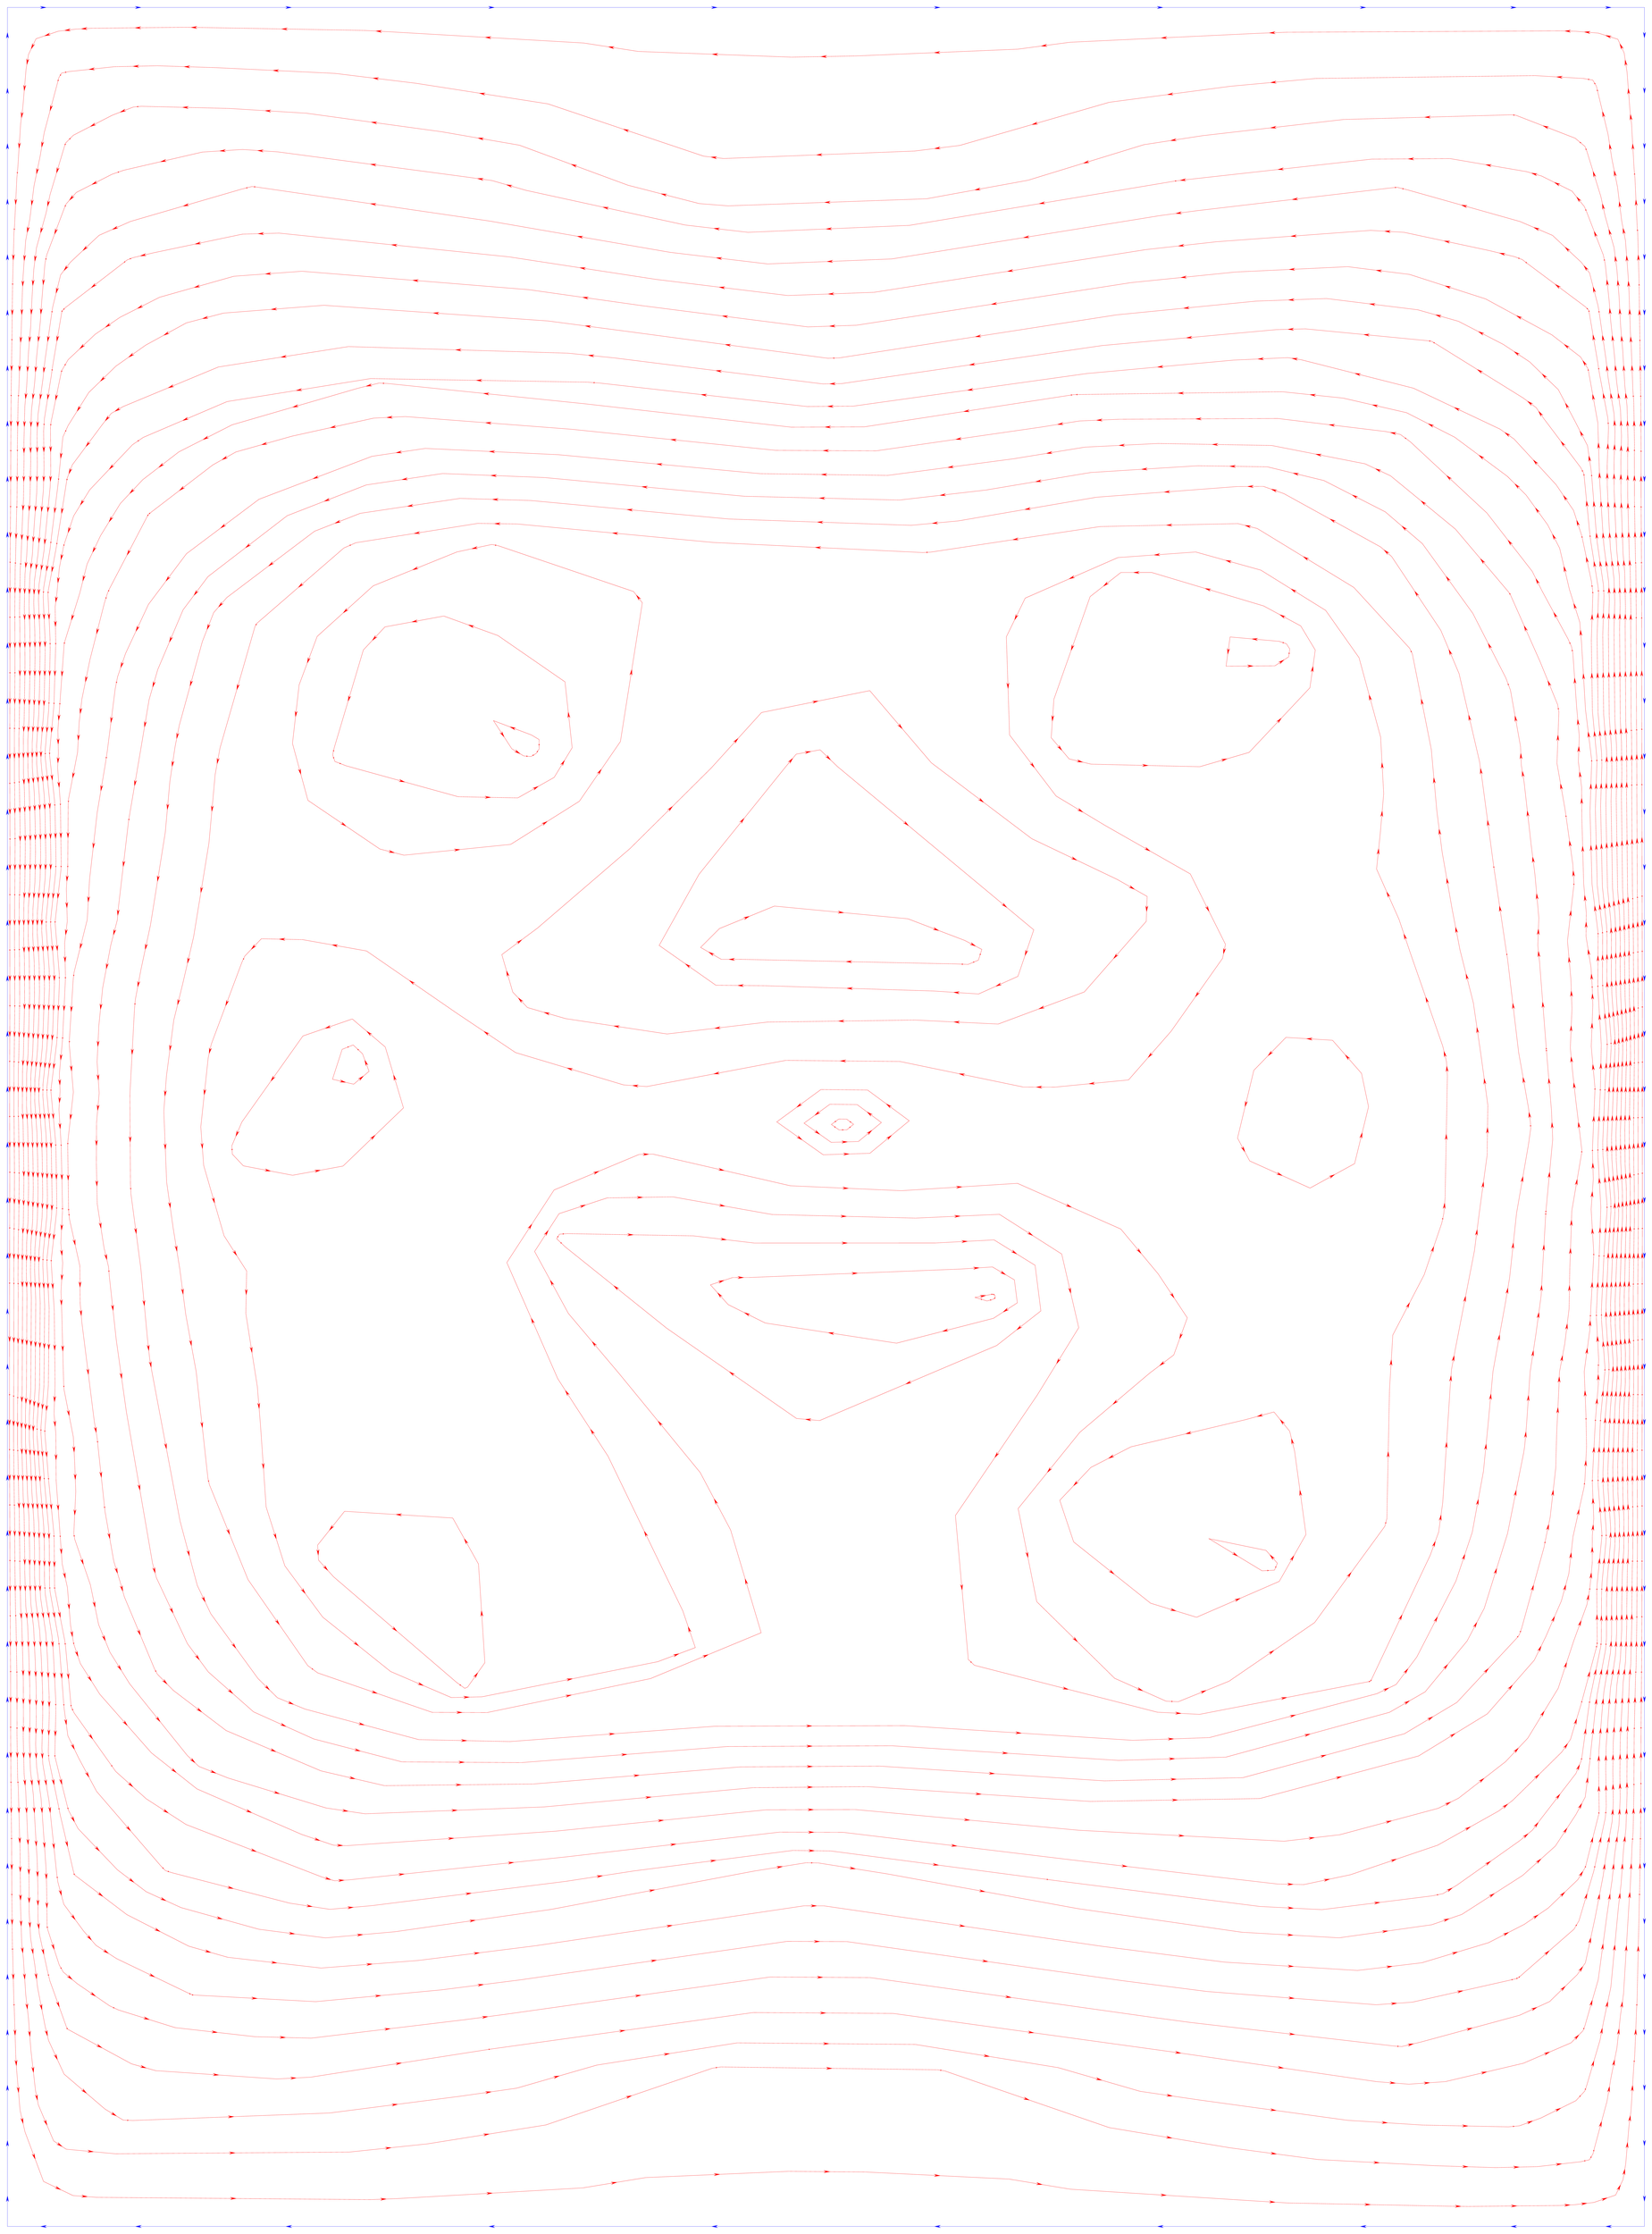
\begin{tikzpicture}
\draw[color=boundaryBlue] (0.0000cm, 84.3534cm)
--(16.9503cm,84.3534cm) node[sloped,pos=0.5,allow upside down]{\ArrowIn}
--(33.8994cm,84.3534cm) node[sloped,pos=0.5,allow upside down]{\ArrowIn}
--(47.8158cm,84.3534cm) node[sloped,pos=0.5,allow upside down]{\ArrowIn}
--(56.7828cm,84.3534cm) node[sloped,pos=0.5,allow upside down]{\ArrowIn}
--(62.2478cm,84.3534cm) node[sloped,pos=0.5,allow upside down]{\ArrowIn}
--(62.2478cm,80.1357cm) node[sloped,pos=0.5,allow upside down]{\ArrowIn}
--(62.2478cm,75.9181cm) node[sloped,pos=0.5,allow upside down]{\ArrowIn}
--(62.2478cm,71.7004cm) node[sloped,pos=0.5,allow upside down]{\ArrowIn}
--(62.2478cm,67.4827cm) node[sloped,pos=0.5,allow upside down]{\ArrowIn}
--(62.2478cm,63.2650cm) node[sloped,pos=0.5,allow upside down]{\ArrowIn}
--(62.2478cm,59.0474cm) node[sloped,pos=0.5,allow upside down]{\ArrowIn}
--(62.2478cm,54.8297cm) node[sloped,pos=0.5,allow upside down]{\ArrowIn}
--(62.2478cm,50.6120cm) node[sloped,pos=0.5,allow upside down]{\ArrowIn}
--(62.2478cm,46.3944cm) node[sloped,pos=0.5,allow upside down]{\ArrowIn}
--(62.2478cm,42.1767cm) node[sloped,pos=0.5,allow upside down]{\ArrowIn}
--(62.2478cm,37.9590cm) node[sloped,pos=0.5,allow upside down]{\ArrowIn}
--(62.2478cm,33.7414cm) node[sloped,pos=0.5,allow upside down]{\ArrowIn}
--(62.2478cm,29.5237cm) node[sloped,pos=0.5,allow upside down]{\ArrowIn}
--(62.2478cm,25.3060cm) node[sloped,pos=0.5,allow upside down]{\ArrowIn}
--(62.2478cm,21.0883cm) node[sloped,pos=0.5,allow upside down]{\ArrowIn}
--(62.2478cm,16.8707cm) node[sloped,pos=0.5,allow upside down]{\ArrowIn}
--(62.2478cm,12.6530cm) node[sloped,pos=0.5,allow upside down]{\ArrowIn}
--(62.2478cm,8.4353cm) node[sloped,pos=0.5,allow upside down]{\ArrowIn}
--(62.2478cm,4.2177cm) node[sloped,pos=0.5,allow upside down]{\ArrowIn}
--(62.2478cm,0.0000cm) node[sloped,pos=0.5,allow upside down]{\ArrowIn}
--(62.2478cm,-4.2177cm) node[sloped,pos=0.5,allow upside down]{\ArrowIn}
--(62.2478cm,-8.4353cm) node[sloped,pos=0.5,allow upside down]{\ArrowIn}
--(62.2478cm,-12.6530cm) node[sloped,pos=0.5,allow upside down]{\ArrowIn}
--(62.2478cm,-16.8707cm) node[sloped,pos=0.5,allow upside down]{\ArrowIn}
--(62.2478cm,-21.0883cm) node[sloped,pos=0.5,allow upside down]{\ArrowIn}
--(62.2478cm,-25.3060cm) node[sloped,pos=0.5,allow upside down]{\ArrowIn}
--(62.2478cm,-29.5237cm) node[sloped,pos=0.5,allow upside down]{\ArrowIn}
--(62.2478cm,-33.7414cm) node[sloped,pos=0.5,allow upside down]{\ArrowIn}
--(62.2478cm,-37.9590cm) node[sloped,pos=0.5,allow upside down]{\ArrowIn}
--(62.2478cm,-42.1767cm) node[sloped,pos=0.5,allow upside down]{\ArrowIn}
--(62.2478cm,-46.3944cm) node[sloped,pos=0.5,allow upside down]{\ArrowIn}
--(62.2478cm,-50.6120cm) node[sloped,pos=0.5,allow upside down]{\ArrowIn}
--(62.2478cm,-54.8297cm) node[sloped,pos=0.5,allow upside down]{\ArrowIn}
--(62.2478cm,-59.0474cm) node[sloped,pos=0.5,allow upside down]{\ArrowIn}
--(62.2478cm,-63.2650cm) node[sloped,pos=0.5,allow upside down]{\ArrowIn}
--(62.2478cm,-67.4827cm) node[sloped,pos=0.5,allow upside down]{\ArrowIn}
--(62.2478cm,-71.7004cm) node[sloped,pos=0.5,allow upside down]{\ArrowIn}
--(62.2478cm,-75.9181cm) node[sloped,pos=0.5,allow upside down]{\ArrowIn}
--(62.2478cm,-80.1357cm) node[sloped,pos=0.5,allow upside down]{\ArrowIn}
--(62.2478cm,-84.3534cm) node[sloped,pos=0.5,allow upside down]{\ArrowIn}
--(56.7828cm,-84.3534cm) node[sloped,pos=0.5,allow upside down]{\ArrowIn}
--(47.8158cm,-84.3534cm) node[sloped,pos=0.5,allow upside down]{\ArrowIn}
--(33.8994cm,-84.3534cm) node[sloped,pos=0.5,allow upside down]{\ArrowIn}
--(16.9503cm,-84.3534cm) node[sloped,pos=0.5,allow upside down]{\ArrowIn}
--(-0.0000cm,-84.3534cm) node[sloped,pos=0.5,allow upside down]{\ArrowIn}
--(-16.9503cm,-84.3534cm) node[sloped,pos=0.5,allow upside down]{\ArrowIn}
--(-33.8994cm,-84.3534cm) node[sloped,pos=0.5,allow upside down]{\ArrowIn}
--(-47.8158cm,-84.3534cm) node[sloped,pos=0.5,allow upside down]{\ArrowIn}
--(-56.7828cm,-84.3534cm) node[sloped,pos=0.5,allow upside down]{\ArrowIn}
--(-62.2478cm,-84.3534cm) node[sloped,pos=0.5,allow upside down]{\ArrowIn}
--(-62.2478cm,-80.1357cm) node[sloped,pos=0.5,allow upside down]{\ArrowIn}
--(-62.2478cm,-75.9181cm) node[sloped,pos=0.5,allow upside down]{\ArrowIn}
--(-62.2478cm,-71.7004cm) node[sloped,pos=0.5,allow upside down]{\ArrowIn}
--(-62.2478cm,-67.4827cm) node[sloped,pos=0.5,allow upside down]{\ArrowIn}
--(-62.2478cm,-63.2650cm) node[sloped,pos=0.5,allow upside down]{\ArrowIn}
--(-62.2478cm,-59.0474cm) node[sloped,pos=0.5,allow upside down]{\ArrowIn}
--(-62.2478cm,-54.8297cm) node[sloped,pos=0.5,allow upside down]{\ArrowIn}
--(-62.2478cm,-50.6120cm) node[sloped,pos=0.5,allow upside down]{\ArrowIn}
--(-62.2478cm,-46.3944cm) node[sloped,pos=0.5,allow upside down]{\ArrowIn}
--(-62.2478cm,-42.1767cm) node[sloped,pos=0.5,allow upside down]{\ArrowIn}
--(-62.2478cm,-37.9590cm) node[sloped,pos=0.5,allow upside down]{\ArrowIn}
--(-62.2478cm,-33.7414cm) node[sloped,pos=0.5,allow upside down]{\ArrowIn}
--(-62.2478cm,-29.5237cm) node[sloped,pos=0.5,allow upside down]{\ArrowIn}
--(-62.2478cm,-25.3060cm) node[sloped,pos=0.5,allow upside down]{\ArrowIn}
--(-62.2478cm,-21.0883cm) node[sloped,pos=0.5,allow upside down]{\ArrowIn}
--(-62.2478cm,-16.8707cm) node[sloped,pos=0.5,allow upside down]{\ArrowIn}
--(-62.2478cm,-12.6530cm) node[sloped,pos=0.5,allow upside down]{\ArrowIn}
--(-62.2478cm,-8.4353cm) node[sloped,pos=0.5,allow upside down]{\ArrowIn}
--(-62.2478cm,-4.2177cm) node[sloped,pos=0.5,allow upside down]{\ArrowIn}
--(-62.2478cm,0.0000cm) node[sloped,pos=0.5,allow upside down]{\ArrowIn}
--(-62.2478cm,4.2177cm) node[sloped,pos=0.5,allow upside down]{\ArrowIn}
--(-62.2478cm,8.4353cm) node[sloped,pos=0.5,allow upside down]{\ArrowIn}
--(-62.2478cm,12.6530cm) node[sloped,pos=0.5,allow upside down]{\ArrowIn}
--(-62.2478cm,16.8707cm) node[sloped,pos=0.5,allow upside down]{\ArrowIn}
--(-62.2478cm,21.0883cm) node[sloped,pos=0.5,allow upside down]{\ArrowIn}
--(-62.2478cm,25.3060cm) node[sloped,pos=0.5,allow upside down]{\ArrowIn}
--(-62.2478cm,29.5237cm) node[sloped,pos=0.5,allow upside down]{\ArrowIn}
--(-62.2478cm,33.7414cm) node[sloped,pos=0.5,allow upside down]{\ArrowIn}
--(-62.2478cm,37.9590cm) node[sloped,pos=0.5,allow upside down]{\ArrowIn}
--(-62.2478cm,42.1767cm) node[sloped,pos=0.5,allow upside down]{\ArrowIn}
--(-62.2478cm,46.3944cm) node[sloped,pos=0.5,allow upside down]{\ArrowIn}
--(-62.2478cm,50.6120cm) node[sloped,pos=0.5,allow upside down]{\ArrowIn}
--(-62.2478cm,54.8297cm) node[sloped,pos=0.5,allow upside down]{\ArrowIn}
--(-62.2478cm,59.0474cm) node[sloped,pos=0.5,allow upside down]{\ArrowIn}
--(-62.2478cm,63.2650cm) node[sloped,pos=0.5,allow upside down]{\ArrowIn}
--(-62.2478cm,67.4827cm) node[sloped,pos=0.5,allow upside down]{\ArrowIn}
--(-62.2478cm,71.7004cm) node[sloped,pos=0.5,allow upside down]{\ArrowIn}
--(-62.2478cm,75.9181cm) node[sloped,pos=0.5,allow upside down]{\ArrowIn}
--(-62.2478cm,80.1357cm) node[sloped,pos=0.5,allow upside down]{\ArrowIn}
--(-62.2478cm,84.3534cm) node[sloped,pos=0.5,allow upside down]{\ArrowIn}
--(-56.7828cm,84.3534cm) node[sloped,pos=0.5,allow upside down]{\ArrowIn}
--(-47.8158cm,84.3534cm) node[sloped,pos=0.5,allow upside down]{\ArrowIn}
--(-33.8994cm,84.3534cm) node[sloped,pos=0.5,allow upside down]{\ArrowIn}
--(-16.9503cm,84.3534cm) node[sloped,pos=0.5,allow upside down]{\ArrowIn}
--(0.0000cm,84.3534cm) node[sloped,pos=0.5,allow upside down]{\ArrowIn}
--cycle;

\draw[color=wireRed] (0.9748cm, -0.1577cm)
--(0.4119cm,-0.5701cm) node[sloped,pos=0.5,allow upside down]{\arrowIn}
--(1.0040cm,-0.9890cm) node[sloped,pos=0.5,allow upside down]{\arrowIn}
--(1.5989cm,-0.9706cm) node[sloped,pos=0.5,allow upside down]{\arrowIn}
--(2.1006cm,-0.5556cm) node[sloped,pos=0.5,allow upside down]{\arrowIn}
--(1.5702cm,-0.1641cm) node[sloped,pos=0.5,allow upside down]{\arrowIn}
--cycle;
\draw[color=wireRed] (35.0233cm, 35.9742cm)
--(34.4699cm,36.1611cm) node[sloped,pos=0.5,allow upside down]{\arrowIn}
--(30.7358cm,36.4949cm) node[sloped,pos=0.5,allow upside down]{\ArrowIn}
--(30.4298cm,34.2743cm) node[sloped,pos=0.5,allow upside down]{\ArrowIn}
--(34.1456cm,34.2984cm) node[sloped,pos=0.5,allow upside down]{\ArrowIn}
--(35.1908cm,34.9807cm) node[sloped,pos=0.5,allow upside down]{\ArrowIn}
--(35.2741cm,35.5808cm) node[sloped,pos=0.5,allow upside down]{\arrowIn}
--cycle;
\draw[color=wireRed] (-22.3983cm, 29.0420cm)
--(-25.2824cm,30.1300cm) node[sloped,pos=0.5,allow upside down]{\ArrowIn}
--(-23.8928cm,27.9947cm) node[sloped,pos=0.5,allow upside down]{\ArrowIn}
--(-22.9850cm,27.4480cm) node[sloped,pos=0.5,allow upside down]{\ArrowIn}
--(-22.4357cm,27.4013cm) node[sloped,pos=0.5,allow upside down]{\arrowIn}
--(-22.0405cm,27.6355cm) node[sloped,pos=0.5,allow upside down]{\arrowIn}
--(-21.8158cm,27.9762cm) node[sloped,pos=0.5,allow upside down]{\arrowIn}
--(-21.8206cm,28.6974cm) node[sloped,pos=0.5,allow upside down]{\arrowIn}
--cycle;
\draw[color=wireRed] (0.2955cm, 0.9635cm)
--(-1.6646cm,-0.4728cm) node[sloped,pos=0.5,allow upside down]{\ArrowIn}
--(0.3973cm,-1.9314cm) node[sloped,pos=0.5,allow upside down]{\ArrowIn}
--(2.4690cm,-1.8673cm) node[sloped,pos=0.5,allow upside down]{\ArrowIn}
--(4.2164cm,-0.4224cm) node[sloped,pos=0.5,allow upside down]{\ArrowIn}
--(2.3691cm,0.9412cm) node[sloped,pos=0.5,allow upside down]{\ArrowIn}
--cycle;
\draw[color=wireRed] (29.1298cm, -32.0613cm)
--(33.1664cm,-34.5056cm) node[sloped,pos=0.5,allow upside down]{\ArrowIn}
--(34.1109cm,-34.4565cm) node[sloped,pos=0.5,allow upside down]{\arrowIn}
--(34.3332cm,-33.9276cm) node[sloped,pos=0.5,allow upside down]{\arrowIn}
--(33.4719cm,-32.9553cm) node[sloped,pos=0.5,allow upside down]{\ArrowIn}
--cycle;
\draw[color=wireRed] (-37.5292cm, 2.8688cm)
--(-35.9159cm,2.4907cm) node[sloped,pos=0.5,allow upside down]{\ArrowIn}
--(-34.7478cm,3.4675cm) node[sloped,pos=0.5,allow upside down]{\ArrowIn}
--(-35.2456cm,4.8054cm) node[sloped,pos=0.5,allow upside down]{\ArrowIn}
--(-35.9557cm,5.4743cm) node[sloped,pos=0.5,allow upside down]{\arrowIn}
--(-36.7925cm,5.1416cm) node[sloped,pos=0.5,allow upside down]{\arrowIn}
--cycle;
\draw[color=wireRed] (36.1096cm, 37.3334cm)
--(33.2865cm,38.8522cm) node[sloped,pos=0.5,allow upside down]{\ArrowIn}
--(24.7768cm,41.3960cm) node[sloped,pos=0.5,allow upside down]{\ArrowIn}
--(22.4279cm,41.3937cm) node[sloped,pos=0.5,allow upside down]{\ArrowIn}
--(20.0936cm,39.5632cm) node[sloped,pos=0.5,allow upside down]{\ArrowIn}
--(17.3360cm,31.7551cm) node[sloped,pos=0.5,allow upside down]{\ArrowIn}
--(17.1312cm,28.8360cm) node[sloped,pos=0.5,allow upside down]{\ArrowIn}
--(18.4985cm,27.2196cm) node[sloped,pos=0.5,allow upside down]{\ArrowIn}
--(20.1692cm,26.8238cm) node[sloped,pos=0.5,allow upside down]{\ArrowIn}
--(28.4323cm,26.6289cm) node[sloped,pos=0.5,allow upside down]{\ArrowIn}
--(32.1857cm,27.7173cm) node[sloped,pos=0.5,allow upside down]{\ArrowIn}
--(36.8064cm,32.6303cm) node[sloped,pos=0.5,allow upside down]{\ArrowIn}
--(37.2147cm,35.4973cm) node[sloped,pos=0.5,allow upside down]{\ArrowIn}
--cycle;
\draw[color=wireRed] (-24.9495cm, 36.6026cm)
--(-29.0599cm,38.0829cm) node[sloped,pos=0.5,allow upside down]{\ArrowIn}
--(-33.5383cm,37.2576cm) node[sloped,pos=0.5,allow upside down]{\ArrowIn}
--(-35.1811cm,35.5046cm) node[sloped,pos=0.5,allow upside down]{\ArrowIn}
--(-37.3911cm,28.0876cm) node[sloped,pos=0.5,allow upside down]{\ArrowIn}
--(-37.5177cm,27.5327cm) node[sloped,pos=0.5,allow upside down]{\arrowIn}
--(-37.3447cm,27.0261cm) node[sloped,pos=0.5,allow upside down]{\arrowIn}
--(-36.4843cm,26.6957cm) node[sloped,pos=0.5,allow upside down]{\arrowIn}
--(-27.9679cm,24.3471cm) node[sloped,pos=0.5,allow upside down]{\ArrowIn}
--(-23.4347cm,24.2581cm) node[sloped,pos=0.5,allow upside down]{\ArrowIn}
--(-20.6704cm,25.8156cm) node[sloped,pos=0.5,allow upside down]{\ArrowIn}
--(-19.3001cm,28.0709cm) node[sloped,pos=0.5,allow upside down]{\ArrowIn}
--(-19.8465cm,33.0805cm) node[sloped,pos=0.5,allow upside down]{\ArrowIn}
--cycle;
\draw[color=wireRed] (40.7325cm, 3.3125cm)
--(38.5270cm,5.8299cm) node[sloped,pos=0.5,allow upside down]{\ArrowIn}
--(34.9867cm,6.0509cm) node[sloped,pos=0.5,allow upside down]{\ArrowIn}
--(32.5424cm,3.5452cm) node[sloped,pos=0.5,allow upside down]{\ArrowIn}
--(31.3027cm,-1.6058cm) node[sloped,pos=0.5,allow upside down]{\ArrowIn}
--(32.2294cm,-3.3457cm) node[sloped,pos=0.5,allow upside down]{\ArrowIn}
--(36.8166cm,-5.4070cm) node[sloped,pos=0.5,allow upside down]{\ArrowIn}
--(40.2057cm,-3.5483cm) node[sloped,pos=0.5,allow upside down]{\ArrowIn}
--(41.2658cm,0.7766cm) node[sloped,pos=0.5,allow upside down]{\ArrowIn}
--cycle;
\draw[color=wireRed] (-0.3837cm, 2.0846cm)
--(-3.7412cm,-0.3754cm) node[sloped,pos=0.5,allow upside down]{\ArrowIn}
--(-0.2094cm,-2.8739cm) node[sloped,pos=0.5,allow upside down]{\ArrowIn}
--(3.3392cm,-2.7640cm) node[sloped,pos=0.5,allow upside down]{\ArrowIn}
--(6.3321cm,-0.2891cm) node[sloped,pos=0.5,allow upside down]{\ArrowIn}
--(3.1681cm,2.0466cm) node[sloped,pos=0.5,allow upside down]{\ArrowIn}
--cycle;
\draw[color=wireRed] (18.8376cm, -32.3063cm)
--(24.6898cm,-36.9681cm) node[sloped,pos=0.5,allow upside down]{\ArrowIn}
--(28.1866cm,-38.0380cm) node[sloped,pos=0.5,allow upside down]{\ArrowIn}
--(34.4745cm,-35.3097cm) node[sloped,pos=0.5,allow upside down]{\ArrowIn}
--(36.5089cm,-31.7389cm) node[sloped,pos=0.5,allow upside down]{\ArrowIn}
--(35.6394cm,-25.3995cm) node[sloped,pos=0.5,allow upside down]{\ArrowIn}
--(35.2679cm,-23.8937cm) node[sloped,pos=0.5,allow upside down]{\ArrowIn}
--(34.0740cm,-22.4277cm) node[sloped,pos=0.5,allow upside down]{\ArrowIn}
--(31.9097cm,-23.0136cm) node[sloped,pos=0.5,allow upside down]{\ArrowIn}
--(23.1974cm,-25.0797cm) node[sloped,pos=0.5,allow upside down]{\ArrowIn}
--(20.1456cm,-26.6467cm) node[sloped,pos=0.5,allow upside down]{\ArrowIn}
--(17.7829cm,-29.1473cm) node[sloped,pos=0.5,allow upside down]{\ArrowIn}
--cycle;
\draw[color=wireRed] (-27.2506cm, -43.3439cm)
--(-25.9390cm,-41.4896cm) node[sloped,pos=0.5,allow upside down]{\ArrowIn}
--(-26.4252cm,-33.9922cm) node[sloped,pos=0.5,allow upside down]{\ArrowIn}
--(-28.3829cm,-30.4917cm) node[sloped,pos=0.5,allow upside down]{\ArrowIn}
--(-36.6101cm,-29.9804cm) node[sloped,pos=0.5,allow upside down]{\ArrowIn}
--(-38.6587cm,-32.5488cm) node[sloped,pos=0.5,allow upside down]{\ArrowIn}
--(-38.5911cm,-33.6922cm) node[sloped,pos=0.5,allow upside down]{\ArrowIn}
--(-37.4483cm,-34.9579cm) node[sloped,pos=0.5,allow upside down]{\ArrowIn}
--(-28.1064cm,-42.9758cm) node[sloped,pos=0.5,allow upside down]{\ArrowIn}
--(-27.4675cm,-43.4404cm) node[sloped,pos=0.5,allow upside down]{\arrowIn}
--cycle;
\draw[color=wireRed] (-44.3060cm, -3.7165cm)
--(-40.5607cm,-4.4334cm) node[sloped,pos=0.5,allow upside down]{\ArrowIn}
--(-36.7266cm,-3.7341cm) node[sloped,pos=0.5,allow upside down]{\ArrowIn}
--(-32.1305cm,0.6885cm) node[sloped,pos=0.5,allow upside down]{\ArrowIn}
--(-33.5150cm,5.3186cm) node[sloped,pos=0.5,allow upside down]{\ArrowIn}
--(-36.0226cm,7.4496cm) node[sloped,pos=0.5,allow upside down]{\ArrowIn}
--(-39.7775cm,6.1569cm) node[sloped,pos=0.5,allow upside down]{\ArrowIn}
--(-44.4229cm,-0.3873cm) node[sloped,pos=0.5,allow upside down]{\ArrowIn}
--(-45.1804cm,-2.1851cm) node[sloped,pos=0.5,allow upside down]{\ArrowIn}
--(-45.1462cm,-2.8291cm) node[sloped,pos=0.5,allow upside down]{\arrowIn}
--cycle;
\draw[color=wireRed] (38.0062cm, 38.5135cm)
--(33.0759cm,41.5743cm) node[sloped,pos=0.5,allow upside down]{\ArrowIn}
--(28.1233cm,42.9534cm) node[sloped,pos=0.5,allow upside down]{\ArrowIn}
--(22.2041cm,42.5294cm) node[sloped,pos=0.5,allow upside down]{\ArrowIn}
--(15.1538cm,39.4463cm) node[sloped,pos=0.5,allow upside down]{\ArrowIn}
--(13.7198cm,36.5024cm) node[sloped,pos=0.5,allow upside down]{\ArrowIn}
--(13.9668cm,29.0419cm) node[sloped,pos=0.5,allow upside down]{\ArrowIn}
--(17.5017cm,24.4020cm) node[sloped,pos=0.5,allow upside down]{\ArrowIn}
--(21.2497cm,22.1519cm) node[sloped,pos=0.5,allow upside down]{\ArrowIn}
--(27.7094cm,18.4783cm) node[sloped,pos=0.5,allow upside down]{\ArrowIn}
--(30.3839cm,13.1269cm) node[sloped,pos=0.5,allow upside down]{\ArrowIn}
--(30.1651cm,12.0633cm) node[sloped,pos=0.5,allow upside down]{\ArrowIn}
--(26.2501cm,6.5164cm) node[sloped,pos=0.5,allow upside down]{\ArrowIn}
--(23.0118cm,2.8155cm) node[sloped,pos=0.5,allow upside down]{\ArrowIn}
--(17.3971cm,2.2670cm) node[sloped,pos=0.5,allow upside down]{\ArrowIn}
--(15.0057cm,2.2756cm) node[sloped,pos=0.5,allow upside down]{\ArrowIn}
--(5.6371cm,4.2167cm) node[sloped,pos=0.5,allow upside down]{\ArrowIn}
--(-3.0567cm,4.3014cm) node[sloped,pos=0.5,allow upside down]{\ArrowIn}
--(-13.6197cm,2.3110cm) node[sloped,pos=0.5,allow upside down]{\ArrowIn}
--(-15.3898cm,2.4369cm) node[sloped,pos=0.5,allow upside down]{\ArrowIn}
--(-23.6045cm,4.8946cm) node[sloped,pos=0.5,allow upside down]{\ArrowIn}
--(-28.0867cm,7.8962cm) node[sloped,pos=0.5,allow upside down]{\ArrowIn}
--(-34.9394cm,12.6205cm) node[sloped,pos=0.5,allow upside down]{\ArrowIn}
--(-39.7937cm,13.4810cm) node[sloped,pos=0.5,allow upside down]{\ArrowIn}
--(-42.9392cm,13.5478cm) node[sloped,pos=0.5,allow upside down]{\ArrowIn}
--(-44.1966cm,12.2315cm) node[sloped,pos=0.5,allow upside down]{\ArrowIn}
--(-44.4234cm,11.7456cm) node[sloped,pos=0.5,allow upside down]{\arrowIn}
--(-46.7471cm,5.5322cm) node[sloped,pos=0.5,allow upside down]{\ArrowIn}
--(-46.9795cm,4.5069cm) node[sloped,pos=0.5,allow upside down]{\ArrowIn}
--(-47.5450cm,-0.7564cm) node[sloped,pos=0.5,allow upside down]{\ArrowIn}
--(-47.3258cm,-3.6821cm) node[sloped,pos=0.5,allow upside down]{\ArrowIn}
--(-45.7747cm,-9.0323cm) node[sloped,pos=0.5,allow upside down]{\ArrowIn}
--(-44.0566cm,-11.7145cm) node[sloped,pos=0.5,allow upside down]{\ArrowIn}
--(-44.1200cm,-14.9411cm) node[sloped,pos=0.5,allow upside down]{\ArrowIn}
--(-43.2437cm,-20.4960cm) node[sloped,pos=0.5,allow upside down]{\ArrowIn}
--(-43.0027cm,-23.4549cm) node[sloped,pos=0.5,allow upside down]{\ArrowIn}
--(-42.5755cm,-29.6497cm) node[sloped,pos=0.5,allow upside down]{\ArrowIn}
--(-41.1536cm,-34.1261cm) node[sloped,pos=0.5,allow upside down]{\ArrowIn}
--(-38.2754cm,-38.0229cm) node[sloped,pos=0.5,allow upside down]{\ArrowIn}
--(-33.1069cm,-42.1628cm) node[sloped,pos=0.5,allow upside down]{\ArrowIn}
--(-28.4879cm,-44.1429cm) node[sloped,pos=0.5,allow upside down]{\ArrowIn}
--(-26.1627cm,-44.0860cm) node[sloped,pos=0.5,allow upside down]{\ArrowIn}
--(-12.7926cm,-41.4155cm) node[sloped,pos=0.5,allow upside down]{\ArrowIn}
--(-9.9351cm,-40.3440cm) node[sloped,pos=0.5,allow upside down]{\ArrowIn}
--(-10.8866cm,-37.5518cm) node[sloped,pos=0.5,allow upside down]{\ArrowIn}
--(-16.5723cm,-25.7931cm) node[sloped,pos=0.5,allow upside down]{\ArrowIn}
--(-19.0211cm,-22.0276cm) node[sloped,pos=0.5,allow upside down]{\ArrowIn}
--(-20.3989cm,-19.8947cm) node[sloped,pos=0.5,allow upside down]{\ArrowIn}
--(-24.2686cm,-11.0688cm) node[sloped,pos=0.5,allow upside down]{\ArrowIn}
--(-20.6773cm,-5.5520cm) node[sloped,pos=0.5,allow upside down]{\ArrowIn}
--(-14.2144cm,-2.8502cm) node[sloped,pos=0.5,allow upside down]{\ArrowIn}
--(-13.1470cm,-2.8278cm) node[sloped,pos=0.5,allow upside down]{\ArrowIn}
--(-2.7126cm,-5.2304cm) node[sloped,pos=0.5,allow upside down]{\ArrowIn}
--(5.7315cm,-5.6067cm) node[sloped,pos=0.5,allow upside down]{\ArrowIn}
--(14.5656cm,-5.0466cm) node[sloped,pos=0.5,allow upside down]{\ArrowIn}
--(22.4256cm,-8.5220cm) node[sloped,pos=0.5,allow upside down]{\ArrowIn}
--(25.2654cm,-11.9279cm) node[sloped,pos=0.5,allow upside down]{\ArrowIn}
--(27.4829cm,-15.2705cm) node[sloped,pos=0.5,allow upside down]{\ArrowIn}
--(26.4527cm,-18.0952cm) node[sloped,pos=0.5,allow upside down]{\ArrowIn}
--(24.6278cm,-19.4690cm) node[sloped,pos=0.5,allow upside down]{\ArrowIn}
--(19.3082cm,-23.9740cm) node[sloped,pos=0.5,allow upside down]{\ArrowIn}
--(14.6169cm,-29.7729cm) node[sloped,pos=0.5,allow upside down]{\ArrowIn}
--(16.0335cm,-36.8530cm) node[sloped,pos=0.5,allow upside down]{\ArrowIn}
--(21.9539cm,-42.6755cm) node[sloped,pos=0.5,allow upside down]{\ArrowIn}
--(25.8763cm,-44.4196cm) node[sloped,pos=0.5,allow upside down]{\ArrowIn}
--(26.8034cm,-44.4548cm) node[sloped,pos=0.5,allow upside down]{\arrowIn}
--(30.6603cm,-42.8968cm) node[sloped,pos=0.5,allow upside down]{\ArrowIn}
--(37.1647cm,-38.4411cm) node[sloped,pos=0.5,allow upside down]{\ArrowIn}
--(42.5003cm,-31.1272cm) node[sloped,pos=0.5,allow upside down]{\ArrowIn}
--(42.6596cm,-30.5395cm) node[sloped,pos=0.5,allow upside down]{\arrowIn}
--(42.8605cm,-20.7445cm) node[sloped,pos=0.5,allow upside down]{\ArrowIn}
--(43.1108cm,-16.5811cm) node[sloped,pos=0.5,allow upside down]{\ArrowIn}
--(45.4963cm,-12.0001cm) node[sloped,pos=0.5,allow upside down]{\ArrowIn}
--(46.8357cm,-8.0694cm) node[sloped,pos=0.5,allow upside down]{\ArrowIn}
--(46.9893cm,-7.3478cm) node[sloped,pos=0.5,allow upside down]{\arrowIn}
--(47.0887cm,-6.1384cm) node[sloped,pos=0.5,allow upside down]{\ArrowIn}
--(47.2629cm,3.1272cm) node[sloped,pos=0.5,allow upside down]{\ArrowIn}
--(47.1933cm,4.2098cm) node[sloped,pos=0.5,allow upside down]{\ArrowIn}
--(46.9102cm,5.3841cm) node[sloped,pos=0.5,allow upside down]{\ArrowIn}
--(44.4528cm,12.4437cm) node[sloped,pos=0.5,allow upside down]{\ArrowIn}
--(43.5859cm,15.0184cm) node[sloped,pos=0.5,allow upside down]{\ArrowIn}
--(41.8762cm,18.8506cm) node[sloped,pos=0.5,allow upside down]{\ArrowIn}
--(42.1555cm,21.5325cm) node[sloped,pos=0.5,allow upside down]{\ArrowIn}
--(42.4185cm,24.5847cm) node[sloped,pos=0.5,allow upside down]{\ArrowIn}
--(42.1847cm,28.8831cm) node[sloped,pos=0.5,allow upside down]{\ArrowIn}
--(40.5421cm,34.9203cm) node[sloped,pos=0.5,allow upside down]{\ArrowIn}
--cycle;
\draw[color=wireRed] (-24.9021cm, 43.4237cm)
--(-25.4051cm,43.5265cm) node[sloped,pos=0.5,allow upside down]{\arrowIn}
--(-28.0633cm,42.9574cm) node[sloped,pos=0.5,allow upside down]{\ArrowIn}
--(-34.4351cm,40.3798cm) node[sloped,pos=0.5,allow upside down]{\ArrowIn}
--(-38.6925cm,36.5363cm) node[sloped,pos=0.5,allow upside down]{\ArrowIn}
--(-40.0651cm,32.8526cm) node[sloped,pos=0.5,allow upside down]{\ArrowIn}
--(-40.5719cm,28.3992cm) node[sloped,pos=0.5,allow upside down]{\ArrowIn}
--(-39.3973cm,24.0734cm) node[sloped,pos=0.5,allow upside down]{\ArrowIn}
--(-33.9257cm,20.3707cm) node[sloped,pos=0.5,allow upside down]{\ArrowIn}
--(-32.0909cm,19.9013cm) node[sloped,pos=0.5,allow upside down]{\ArrowIn}
--(-23.9759cm,20.7240cm) node[sloped,pos=0.5,allow upside down]{\ArrowIn}
--(-18.7540cm,24.0012cm) node[sloped,pos=0.5,allow upside down]{\ArrowIn}
--(-15.6307cm,28.5435cm) node[sloped,pos=0.5,allow upside down]{\ArrowIn}
--(-13.9638cm,39.0911cm) node[sloped,pos=0.5,allow upside down]{\ArrowIn}
--(-14.6299cm,39.9468cm) node[sloped,pos=0.5,allow upside down]{\ArrowIn}
--cycle;
\draw[color=wireRed] (40.1492cm, 40.2581cm)
--(32.8021cm,44.7401cm) node[sloped,pos=0.5,allow upside down]{\ArrowIn}
--(31.3401cm,45.1119cm) node[sloped,pos=0.5,allow upside down]{\ArrowIn}
--(20.8503cm,44.8868cm) node[sloped,pos=0.5,allow upside down]{\ArrowIn}
--(7.9538cm,42.9410cm) node[sloped,pos=0.5,allow upside down]{\ArrowIn}
--(7.3594cm,42.9117cm) node[sloped,pos=0.5,allow upside down]{\arrowIn}
--(-8.5827cm,43.6786cm) node[sloped,pos=0.5,allow upside down]{\ArrowIn}
--(-23.5125cm,45.0864cm) node[sloped,pos=0.5,allow upside down]{\ArrowIn}
--(-26.4834cm,45.1268cm) node[sloped,pos=0.5,allow upside down]{\ArrowIn}
--(-35.7517cm,43.6559cm) node[sloped,pos=0.5,allow upside down]{\ArrowIn}
--(-36.6617cm,43.2585cm) node[sloped,pos=0.5,allow upside down]{\arrowIn}
--(-43.2794cm,37.5293cm) node[sloped,pos=0.5,allow upside down]{\ArrowIn}
--(-43.4220cm,37.2915cm) node[sloped,pos=0.5,allow upside down]{\arrowIn}
--(-46.0827cm,28.0548cm) node[sloped,pos=0.5,allow upside down]{\ArrowIn}
--(-46.4508cm,26.0464cm) node[sloped,pos=0.5,allow upside down]{\ArrowIn}
--(-46.9268cm,20.8060cm) node[sloped,pos=0.5,allow upside down]{\ArrowIn}
--(-48.0912cm,13.6907cm) node[sloped,pos=0.5,allow upside down]{\ArrowIn}
--(-48.9335cm,10.0656cm) node[sloped,pos=0.5,allow upside down]{\ArrowIn}
--(-49.5978cm,7.3643cm) node[sloped,pos=0.5,allow upside down]{\ArrowIn}
--(-50.1554cm,3.1251cm) node[sloped,pos=0.5,allow upside down]{\ArrowIn}
--(-50.3565cm,0.4354cm) node[sloped,pos=0.5,allow upside down]{\ArrowIn}
--(-50.1416cm,-4.9547cm) node[sloped,pos=0.5,allow upside down]{\ArrowIn}
--(-49.6393cm,-8.4839cm) node[sloped,pos=0.5,allow upside down]{\ArrowIn}
--(-49.1415cm,-11.5591cm) node[sloped,pos=0.5,allow upside down]{\ArrowIn}
--(-48.6882cm,-15.0193cm) node[sloped,pos=0.5,allow upside down]{\ArrowIn}
--(-47.8926cm,-19.3845cm) node[sloped,pos=0.5,allow upside down]{\ArrowIn}
--(-47.0017cm,-27.4677cm) node[sloped,pos=0.5,allow upside down]{\ArrowIn}
--(-46.8906cm,-27.9569cm) node[sloped,pos=0.5,allow upside down]{\arrowIn}
--(-43.9525cm,-35.1732cm) node[sloped,pos=0.5,allow upside down]{\ArrowIn}
--(-39.4114cm,-41.7101cm) node[sloped,pos=0.5,allow upside down]{\ArrowIn}
--(-38.6542cm,-42.2660cm) node[sloped,pos=0.5,allow upside down]{\arrowIn}
--(-29.9567cm,-45.2655cm) node[sloped,pos=0.5,allow upside down]{\ArrowIn}
--(-25.7668cm,-45.2823cm) node[sloped,pos=0.5,allow upside down]{\ArrowIn}
--(-13.3426cm,-42.6989cm) node[sloped,pos=0.5,allow upside down]{\ArrowIn}
--(-4.9267cm,-39.2135cm) node[sloped,pos=0.5,allow upside down]{\ArrowIn}
--(-7.2503cm,-31.3997cm) node[sloped,pos=0.5,allow upside down]{\ArrowIn}
--(-9.5620cm,-27.0356cm) node[sloped,pos=0.5,allow upside down]{\ArrowIn}
--(-15.7272cm,-19.5114cm) node[sloped,pos=0.5,allow upside down]{\ArrowIn}
--(-19.5869cm,-14.9405cm) node[sloped,pos=0.5,allow upside down]{\ArrowIn}
--(-22.1569cm,-10.2267cm) node[sloped,pos=0.5,allow upside down]{\ArrowIn}
--(-20.2993cm,-7.3539cm) node[sloped,pos=0.5,allow upside down]{\ArrowIn}
--(-16.6398cm,-6.1538cm) node[sloped,pos=0.5,allow upside down]{\ArrowIn}
--(-11.6373cm,-6.0770cm) node[sloped,pos=0.5,allow upside down]{\ArrowIn}
--(-4.1082cm,-7.4155cm) node[sloped,pos=0.5,allow upside down]{\ArrowIn}
--(6.8277cm,-7.6892cm) node[sloped,pos=0.5,allow upside down]{\ArrowIn}
--(13.1950cm,-7.4024cm) node[sloped,pos=0.5,allow upside down]{\ArrowIn}
--(17.9305cm,-10.4211cm) node[sloped,pos=0.5,allow upside down]{\ArrowIn}
--(19.2251cm,-16.0189cm) node[sloped,pos=0.5,allow upside down]{\ArrowIn}
--(16.0625cm,-21.1590cm) node[sloped,pos=0.5,allow upside down]{\ArrowIn}
--(9.8470cm,-30.2998cm) node[sloped,pos=0.5,allow upside down]{\ArrowIn}
--(10.8260cm,-41.2456cm) node[sloped,pos=0.5,allow upside down]{\ArrowIn}
--(11.2912cm,-41.6879cm) node[sloped,pos=0.5,allow upside down]{\arrowIn}
--(25.2026cm,-45.2552cm) node[sloped,pos=0.5,allow upside down]{\ArrowIn}
--(28.4170cm,-45.4182cm) node[sloped,pos=0.5,allow upside down]{\ArrowIn}
--(41.3015cm,-42.9269cm) node[sloped,pos=0.5,allow upside down]{\ArrowIn}
--(41.4210cm,-42.9002cm) node[sloped,pos=0.5,allow upside down]{\arrowIn}
--(41.5126cm,-42.7194cm) node[sloped,pos=0.5,allow upside down]{\arrowIn}
--(45.9561cm,-33.3246cm) node[sloped,pos=0.5,allow upside down]{\ArrowIn}
--(46.5962cm,-31.5693cm) node[sloped,pos=0.5,allow upside down]{\ArrowIn}
--(46.9070cm,-29.3376cm) node[sloped,pos=0.5,allow upside down]{\ArrowIn}
--(47.4754cm,-20.5279cm) node[sloped,pos=0.5,allow upside down]{\ArrowIn}
--(47.5736cm,-19.2121cm) node[sloped,pos=0.5,allow upside down]{\ArrowIn}
--(47.9017cm,-17.4656cm) node[sloped,pos=0.5,allow upside down]{\ArrowIn}
--(49.3192cm,-10.1787cm) node[sloped,pos=0.5,allow upside down]{\ArrowIn}
--(49.6795cm,-7.3593cm) node[sloped,pos=0.5,allow upside down]{\ArrowIn}
--(50.2845cm,-2.9139cm) node[sloped,pos=0.5,allow upside down]{\ArrowIn}
--(50.3382cm,0.8994cm) node[sloped,pos=0.5,allow upside down]{\ArrowIn}
--(49.8377cm,4.5578cm) node[sloped,pos=0.5,allow upside down]{\ArrowIn}
--(49.2370cm,8.6808cm) node[sloped,pos=0.5,allow upside down]{\ArrowIn}
--(48.2225cm,12.6915cm) node[sloped,pos=0.5,allow upside down]{\ArrowIn}
--(47.6281cm,15.7750cm) node[sloped,pos=0.5,allow upside down]{\ArrowIn}
--(46.8641cm,20.1331cm) node[sloped,pos=0.5,allow upside down]{\ArrowIn}
--(46.4630cm,23.2389cm) node[sloped,pos=0.5,allow upside down]{\ArrowIn}
--(46.0374cm,27.9589cm) node[sloped,pos=0.5,allow upside down]{\ArrowIn}
--(44.5985cm,35.2001cm) node[sloped,pos=0.5,allow upside down]{\ArrowIn}
--(44.3926cm,35.6340cm) node[sloped,pos=0.5,allow upside down]{\arrowIn}
--cycle;
\draw[color=wireRed] (-14.8929cm, 20.4146cm)
--(-8.7321cm,26.5219cm) node[sloped,pos=0.5,allow upside down]{\ArrowIn}
--(-4.9000cm,30.7486cm) node[sloped,pos=0.5,allow upside down]{\ArrowIn}
--(3.3312cm,32.4131cm) node[sloped,pos=0.5,allow upside down]{\ArrowIn}
--(8.0180cm,26.9243cm) node[sloped,pos=0.5,allow upside down]{\ArrowIn}
--(15.6519cm,21.1573cm) node[sloped,pos=0.5,allow upside down]{\ArrowIn}
--(22.1525cm,18.0587cm) node[sloped,pos=0.5,allow upside down]{\ArrowIn}
--(24.4291cm,16.7658cm) node[sloped,pos=0.5,allow upside down]{\ArrowIn}
--(24.3590cm,14.8740cm) node[sloped,pos=0.5,allow upside down]{\ArrowIn}
--(19.6494cm,9.5032cm) node[sloped,pos=0.5,allow upside down]{\ArrowIn}
--(13.1031cm,7.0631cm) node[sloped,pos=0.5,allow upside down]{\ArrowIn}
--(6.7645cm,7.3676cm) node[sloped,pos=0.5,allow upside down]{\ArrowIn}
--(-4.4540cm,7.2135cm) node[sloped,pos=0.5,allow upside down]{\ArrowIn}
--(-12.0833cm,6.3080cm) node[sloped,pos=0.5,allow upside down]{\ArrowIn}
--(-19.7933cm,7.4753cm) node[sloped,pos=0.5,allow upside down]{\ArrowIn}
--(-22.6986cm,8.3184cm) node[sloped,pos=0.5,allow upside down]{\ArrowIn}
--(-23.8173cm,9.4923cm) node[sloped,pos=0.5,allow upside down]{\ArrowIn}
--(-24.6505cm,12.3433cm) node[sloped,pos=0.5,allow upside down]{\ArrowIn}
--(-21.9406cm,14.3572cm) node[sloped,pos=0.5,allow upside down]{\ArrowIn}
--cycle;
\draw[color=wireRed] (53.5991cm, -0.8870cm)
--(53.5771cm,-0.3937cm) node[sloped,pos=0.5,allow upside down]{\arrowIn}
--(53.4220cm,0.7329cm) node[sloped,pos=0.5,allow upside down]{\ArrowIn}
--(52.6824cm,4.9016cm) node[sloped,pos=0.5,allow upside down]{\ArrowIn}
--(51.8386cm,12.0073cm) node[sloped,pos=0.5,allow upside down]{\ArrowIn}
--(51.7175cm,12.7720cm) node[sloped,pos=0.5,allow upside down]{\arrowIn}
--(50.8047cm,18.9196cm) node[sloped,pos=0.5,allow upside down]{\ArrowIn}
--(50.7738cm,19.1361cm) node[sloped,pos=0.5,allow upside down]{\arrowIn}
--(49.9136cm,25.5802cm) node[sloped,pos=0.5,allow upside down]{\ArrowIn}
--(49.7060cm,27.0271cm) node[sloped,pos=0.5,allow upside down]{\ArrowIn}
--(48.1502cm,33.7081cm) node[sloped,pos=0.5,allow upside down]{\ArrowIn}
--(46.7603cm,37.0028cm) node[sloped,pos=0.5,allow upside down]{\ArrowIn}
--(43.0225cm,42.6094cm) node[sloped,pos=0.5,allow upside down]{\ArrowIn}
--(42.1793cm,43.3403cm) node[sloped,pos=0.5,allow upside down]{\ArrowIn}
--(34.8392cm,47.3868cm) node[sloped,pos=0.5,allow upside down]{\ArrowIn}
--(33.2740cm,47.9415cm) node[sloped,pos=0.5,allow upside down]{\ArrowIn}
--(31.2829cm,47.9309cm) node[sloped,pos=0.5,allow upside down]{\ArrowIn}
--(20.5729cm,47.1178cm) node[sloped,pos=0.5,allow upside down]{\ArrowIn}
--(10.0730cm,45.3182cm) node[sloped,pos=0.5,allow upside down]{\ArrowIn}
--(6.4847cm,44.9818cm) node[sloped,pos=0.5,allow upside down]{\ArrowIn}
--(-7.3895cm,45.4619cm) node[sloped,pos=0.5,allow upside down]{\ArrowIn}
--(-22.4743cm,46.8692cm) node[sloped,pos=0.5,allow upside down]{\ArrowIn}
--(-27.8389cm,47.0277cm) node[sloped,pos=0.5,allow upside down]{\ArrowIn}
--(-35.4209cm,45.8919cm) node[sloped,pos=0.5,allow upside down]{\ArrowIn}
--(-38.8960cm,44.5301cm) node[sloped,pos=0.5,allow upside down]{\ArrowIn}
--(-45.5668cm,39.4886cm) node[sloped,pos=0.5,allow upside down]{\ArrowIn}
--(-46.5628cm,38.3485cm) node[sloped,pos=0.5,allow upside down]{\ArrowIn}
--(-47.4291cm,36.1345cm) node[sloped,pos=0.5,allow upside down]{\ArrowIn}
--(-49.1809cm,29.7714cm) node[sloped,pos=0.5,allow upside down]{\ArrowIn}
--(-49.5000cm,28.1559cm) node[sloped,pos=0.5,allow upside down]{\ArrowIn}
--(-49.8947cm,25.5188cm) node[sloped,pos=0.5,allow upside down]{\ArrowIn}
--(-50.2468cm,21.6228cm) node[sloped,pos=0.5,allow upside down]{\ArrowIn}
--(-51.3706cm,14.5947cm) node[sloped,pos=0.5,allow upside down]{\ArrowIn}
--(-52.0861cm,11.2542cm) node[sloped,pos=0.5,allow upside down]{\ArrowIn}
--(-52.5238cm,8.9173cm) node[sloped,pos=0.5,allow upside down]{\ArrowIn}
--(-52.5869cm,8.2090cm) node[sloped,pos=0.5,allow upside down]{\arrowIn}
--(-52.9388cm,1.6737cm) node[sloped,pos=0.5,allow upside down]{\ArrowIn}
--(-52.8930cm,-5.1036cm) node[sloped,pos=0.5,allow upside down]{\ArrowIn}
--(-52.8555cm,-5.8580cm) node[sloped,pos=0.5,allow upside down]{\arrowIn}
--(-52.1043cm,-11.5113cm) node[sloped,pos=0.5,allow upside down]{\ArrowIn}
--(-51.6030cm,-16.8234cm) node[sloped,pos=0.5,allow upside down]{\ArrowIn}
--(-51.4407cm,-18.3150cm) node[sloped,pos=0.5,allow upside down]{\ArrowIn}
--(-51.2664cm,-19.3496cm) node[sloped,pos=0.5,allow upside down]{\ArrowIn}
--(-49.1192cm,-30.7373cm) node[sloped,pos=0.5,allow upside down]{\ArrowIn}
--(-47.8078cm,-35.6236cm) node[sloped,pos=0.5,allow upside down]{\ArrowIn}
--(-46.7806cm,-37.7762cm) node[sloped,pos=0.5,allow upside down]{\ArrowIn}
--(-43.1968cm,-42.6921cm) node[sloped,pos=0.5,allow upside down]{\ArrowIn}
--(-41.7198cm,-44.1540cm) node[sloped,pos=0.5,allow upside down]{\ArrowIn}
--(-39.6227cm,-45.0162cm) node[sloped,pos=0.5,allow upside down]{\ArrowIn}
--(-30.9677cm,-47.3404cm) node[sloped,pos=0.5,allow upside down]{\ArrowIn}
--(-24.0451cm,-47.4885cm) node[sloped,pos=0.5,allow upside down]{\ArrowIn}
--(-8.4955cm,-46.3259cm) node[sloped,pos=0.5,allow upside down]{\ArrowIn}
--(5.9860cm,-46.2774cm) node[sloped,pos=0.5,allow upside down]{\ArrowIn}
--(23.3361cm,-47.3920cm) node[sloped,pos=0.5,allow upside down]{\ArrowIn}
--(29.1612cm,-47.1862cm) node[sloped,pos=0.5,allow upside down]{\ArrowIn}
--(41.9015cm,-43.8475cm) node[sloped,pos=0.5,allow upside down]{\ArrowIn}
--(43.3662cm,-43.1459cm) node[sloped,pos=0.5,allow upside down]{\ArrowIn}
--(44.9333cm,-41.0640cm) node[sloped,pos=0.5,allow upside down]{\ArrowIn}
--(47.9127cm,-35.2799cm) node[sloped,pos=0.5,allow upside down]{\ArrowIn}
--(49.1511cm,-31.5886cm) node[sloped,pos=0.5,allow upside down]{\ArrowIn}
--(50.0043cm,-26.9439cm) node[sloped,pos=0.5,allow upside down]{\ArrowIn}
--(50.3759cm,-23.1865cm) node[sloped,pos=0.5,allow upside down]{\ArrowIn}
--(50.7324cm,-19.3259cm) node[sloped,pos=0.5,allow upside down]{\ArrowIn}
--(51.6665cm,-14.1853cm) node[sloped,pos=0.5,allow upside down]{\ArrowIn}
--(51.9960cm,-12.2145cm) node[sloped,pos=0.5,allow upside down]{\ArrowIn}
--(52.5221cm,-7.3262cm) node[sloped,pos=0.5,allow upside down]{\ArrowIn}
--(53.4258cm,-2.1127cm) node[sloped,pos=0.5,allow upside down]{\ArrowIn}
--cycle;
\draw[color=wireRed] (-9.6466cm, 18.4596cm)
--(-3.0494cm,26.6400cm) node[sloped,pos=0.5,allow upside down]{\ArrowIn}
--(-2.2619cm,27.5836cm) node[sloped,pos=0.5,allow upside down]{\ArrowIn}
--(-0.4425cm,27.9144cm) node[sloped,pos=0.5,allow upside down]{\ArrowIn}
--(0.8553cm,26.6585cm) node[sloped,pos=0.5,allow upside down]{\ArrowIn}
--(11.3984cm,17.8904cm) node[sloped,pos=0.5,allow upside down]{\ArrowIn}
--(15.8054cm,14.2249cm) node[sloped,pos=0.5,allow upside down]{\ArrowIn}
--(14.6009cm,10.6902cm) node[sloped,pos=0.5,allow upside down]{\ArrowIn}
--(11.6106cm,9.3504cm) node[sloped,pos=0.5,allow upside down]{\ArrowIn}
--(8.2200cm,9.5752cm) node[sloped,pos=0.5,allow upside down]{\ArrowIn}
--(-4.6236cm,9.9777cm) node[sloped,pos=0.5,allow upside down]{\ArrowIn}
--(-8.3671cm,10.0119cm) node[sloped,pos=0.5,allow upside down]{\ArrowIn}
--(-12.6840cm,13.0416cm) node[sloped,pos=0.5,allow upside down]{\ArrowIn}
--cycle;
\draw[color=wireRed] (16.3453cm, -14.7477cm)
--(12.9869cm,-17.3748cm) node[sloped,pos=0.5,allow upside down]{\ArrowIn}
--(-0.4841cm,-23.0844cm) node[sloped,pos=0.5,allow upside down]{\ArrowIn}
--(-2.2401cm,-22.9239cm) node[sloped,pos=0.5,allow upside down]{\ArrowIn}
--(-12.1206cm,-16.0536cm) node[sloped,pos=0.5,allow upside down]{\ArrowIn}
--(-19.8454cm,-9.8614cm) node[sloped,pos=0.5,allow upside down]{\ArrowIn}
--(-20.4816cm,-9.2533cm) node[sloped,pos=0.5,allow upside down]{\arrowIn}
--(-20.2614cm,-8.9087cm) node[sloped,pos=0.5,allow upside down]{\arrowIn}
--(-19.6413cm,-8.8707cm) node[sloped,pos=0.5,allow upside down]{\arrowIn}
--(-10.0763cm,-9.0395cm) node[sloped,pos=0.5,allow upside down]{\ArrowIn}
--(-5.4556cm,-9.5858cm) node[sloped,pos=0.5,allow upside down]{\ArrowIn}
--(8.3298cm,-9.5816cm) node[sloped,pos=0.5,allow upside down]{\ArrowIn}
--(12.7866cm,-9.3461cm) node[sloped,pos=0.5,allow upside down]{\ArrowIn}
--(15.9067cm,-11.2779cm) node[sloped,pos=0.5,allow upside down]{\ArrowIn}
--cycle;
\draw[color=wireRed] (53.1479cm, -24.9678cm)
--(53.2873cm,-23.3228cm) node[sloped,pos=0.5,allow upside down]{\ArrowIn}
--(53.5537cm,-19.4017cm) node[sloped,pos=0.5,allow upside down]{\ArrowIn}
--(53.9938cm,-16.5183cm) node[sloped,pos=0.5,allow upside down]{\ArrowIn}
--(54.3912cm,-13.6008cm) node[sloped,pos=0.5,allow upside down]{\ArrowIn}
--(54.4569cm,-12.3746cm) node[sloped,pos=0.5,allow upside down]{\ArrowIn}
--(54.7362cm,-7.4675cm) node[sloped,pos=0.5,allow upside down]{\ArrowIn}
--(54.7495cm,-7.2252cm) node[sloped,pos=0.5,allow upside down]{\arrowIn}
--(54.7637cm,-7.0823cm) node[sloped,pos=0.5,allow upside down]{\arrowIn}
--(55.2721cm,-1.7017cm) node[sloped,pos=0.5,allow upside down]{\ArrowIn}
--(55.1805cm,0.4640cm) node[sloped,pos=0.5,allow upside down]{\ArrowIn}
--(54.7973cm,5.0256cm) node[sloped,pos=0.5,allow upside down]{\ArrowIn}
--(54.7877cm,5.1325cm) node[sloped,pos=0.5,allow upside down]{\arrowIn}
--(54.7760cm,5.3168cm) node[sloped,pos=0.5,allow upside down]{\arrowIn}
--(54.2742cm,11.7619cm) node[sloped,pos=0.5,allow upside down]{\ArrowIn}
--(54.1386cm,13.0343cm) node[sloped,pos=0.5,allow upside down]{\ArrowIn}
--(54.2180cm,15.1343cm) node[sloped,pos=0.5,allow upside down]{\ArrowIn}
--(53.9216cm,18.4310cm) node[sloped,pos=0.5,allow upside down]{\ArrowIn}
--(53.6303cm,20.7195cm) node[sloped,pos=0.5,allow upside down]{\ArrowIn}
--(53.0983cm,25.4494cm) node[sloped,pos=0.5,allow upside down]{\ArrowIn}
--(52.8864cm,26.7345cm) node[sloped,pos=0.5,allow upside down]{\ArrowIn}
--(52.8259cm,28.1601cm) node[sloped,pos=0.5,allow upside down]{\ArrowIn}
--(52.0601cm,32.4438cm) node[sloped,pos=0.5,allow upside down]{\ArrowIn}
--(51.7088cm,33.3790cm) node[sloped,pos=0.5,allow upside down]{\arrowIn}
--(49.1951cm,38.2924cm) node[sloped,pos=0.5,allow upside down]{\ArrowIn}
--(45.3647cm,43.5834cm) node[sloped,pos=0.5,allow upside down]{\ArrowIn}
--(42.5385cm,46.0059cm) node[sloped,pos=0.5,allow upside down]{\ArrowIn}
--(37.8733cm,48.3854cm) node[sloped,pos=0.5,allow upside down]{\ArrowIn}
--(33.5641cm,49.4300cm) node[sloped,pos=0.5,allow upside down]{\ArrowIn}
--(28.2742cm,49.5087cm) node[sloped,pos=0.5,allow upside down]{\ArrowIn}
--(20.1381cm,48.9979cm) node[sloped,pos=0.5,allow upside down]{\ArrowIn}
--(12.1588cm,47.6630cm) node[sloped,pos=0.5,allow upside down]{\ArrowIn}
--(5.5885cm,46.9032cm) node[sloped,pos=0.5,allow upside down]{\ArrowIn}
--(-6.1963cm,47.1908cm) node[sloped,pos=0.5,allow upside down]{\ArrowIn}
--(-21.4104cm,48.6134cm) node[sloped,pos=0.5,allow upside down]{\ArrowIn}
--(-29.1534cm,48.9189cm) node[sloped,pos=0.5,allow upside down]{\ArrowIn}
--(-34.9616cm,48.0503cm) node[sloped,pos=0.5,allow upside down]{\ArrowIn}
--(-40.9722cm,45.7134cm) node[sloped,pos=0.5,allow upside down]{\ArrowIn}
--(-47.0001cm,41.0792cm) node[sloped,pos=0.5,allow upside down]{\ArrowIn}
--(-48.8927cm,38.5552cm) node[sloped,pos=0.5,allow upside down]{\ArrowIn}
--(-50.8176cm,34.0162cm) node[sloped,pos=0.5,allow upside down]{\ArrowIn}
--(-51.4757cm,31.7290cm) node[sloped,pos=0.5,allow upside down]{\ArrowIn}
--(-52.1108cm,27.9495cm) node[sloped,pos=0.5,allow upside down]{\ArrowIn}
--(-52.9909cm,22.7903cm) node[sloped,pos=0.5,allow upside down]{\ArrowIn}
--(-53.0510cm,22.3839cm) node[sloped,pos=0.5,allow upside down]{\arrowIn}
--(-53.7936cm,16.0793cm) node[sloped,pos=0.5,allow upside down]{\ArrowIn}
--(-53.8932cm,14.9753cm) node[sloped,pos=0.5,allow upside down]{\ArrowIn}
--(-54.3871cm,13.0791cm) node[sloped,pos=0.5,allow upside down]{\ArrowIn}
--(-55.0073cm,9.8158cm) node[sloped,pos=0.5,allow upside down]{\ArrowIn}
--(-55.2993cm,6.9311cm) node[sloped,pos=0.5,allow upside down]{\ArrowIn}
--(-55.4313cm,4.1736cm) node[sloped,pos=0.5,allow upside down]{\ArrowIn}
--(-55.2728cm,1.8170cm) node[sloped,pos=0.5,allow upside down]{\ArrowIn}
--(-55.4736cm,-0.4401cm) node[sloped,pos=0.5,allow upside down]{\ArrowIn}
--(-55.4861cm,-3.5315cm) node[sloped,pos=0.5,allow upside down]{\ArrowIn}
--(-55.4199cm,-6.6104cm) node[sloped,pos=0.5,allow upside down]{\ArrowIn}
--(-54.9082cm,-9.9241cm) node[sloped,pos=0.5,allow upside down]{\ArrowIn}
--(-54.5589cm,-11.4085cm) node[sloped,pos=0.5,allow upside down]{\ArrowIn}
--(-54.5032cm,-12.0955cm) node[sloped,pos=0.5,allow upside down]{\arrowIn}
--(-53.9726cm,-16.9552cm) node[sloped,pos=0.5,allow upside down]{\ArrowIn}
--(-53.2016cm,-22.4331cm) node[sloped,pos=0.5,allow upside down]{\ArrowIn}
--(-51.2149cm,-33.9301cm) node[sloped,pos=0.5,allow upside down]{\ArrowIn}
--(-50.9155cm,-35.0469cm) node[sloped,pos=0.5,allow upside down]{\ArrowIn}
--(-48.5623cm,-40.0429cm) node[sloped,pos=0.5,allow upside down]{\ArrowIn}
--(-46.9744cm,-42.1924cm) node[sloped,pos=0.5,allow upside down]{\ArrowIn}
--(-43.5328cm,-45.2287cm) node[sloped,pos=0.5,allow upside down]{\ArrowIn}
--(-38.9557cm,-47.2880cm) node[sloped,pos=0.5,allow upside down]{\ArrowIn}
--(-32.2474cm,-49.0326cm) node[sloped,pos=0.5,allow upside down]{\ArrowIn}
--(-23.1429cm,-49.0865cm) node[sloped,pos=0.5,allow upside down]{\ArrowIn}
--(-7.5039cm,-47.8652cm) node[sloped,pos=0.5,allow upside down]{\ArrowIn}
--(5.0307cm,-47.8093cm) node[sloped,pos=0.5,allow upside down]{\ArrowIn}
--(22.2451cm,-48.9208cm) node[sloped,pos=0.5,allow upside down]{\ArrowIn}
--(30.4138cm,-48.6724cm) node[sloped,pos=0.5,allow upside down]{\ArrowIn}
--(42.8612cm,-45.2626cm) node[sloped,pos=0.5,allow upside down]{\ArrowIn}
--(45.5679cm,-43.7105cm) node[sloped,pos=0.5,allow upside down]{\ArrowIn}
--(48.7615cm,-39.8411cm) node[sloped,pos=0.5,allow upside down]{\ArrowIn}
--(50.0688cm,-37.3489cm) node[sloped,pos=0.5,allow upside down]{\ArrowIn}
--(51.8378cm,-31.6726cm) node[sloped,pos=0.5,allow upside down]{\ArrowIn}
--(53.0750cm,-25.4782cm) node[sloped,pos=0.5,allow upside down]{\ArrowIn}
--cycle;
\draw[color=wireRed] (-8.0998cm, 14.3222cm)
--(-3.9203cm,16.0330cm) node[sloped,pos=0.5,allow upside down]{\ArrowIn}
--(6.2315cm,15.0669cm) node[sloped,pos=0.5,allow upside down]{\ArrowIn}
--(10.5569cm,13.4200cm) node[sloped,pos=0.5,allow upside down]{\ArrowIn}
--(11.8555cm,12.7405cm) node[sloped,pos=0.5,allow upside down]{\ArrowIn}
--(11.5959cm,11.9246cm) node[sloped,pos=0.5,allow upside down]{\arrowIn}
--(10.8173cm,11.5990cm) node[sloped,pos=0.5,allow upside down]{\arrowIn}
--(9.8651cm,11.6342cm) node[sloped,pos=0.5,allow upside down]{\arrowIn}
--(-6.3892cm,11.9820cm) node[sloped,pos=0.5,allow upside down]{\ArrowIn}
--(-7.9537cm,11.9810cm) node[sloped,pos=0.5,allow upside down]{\ArrowIn}
--(-9.5309cm,12.8904cm) node[sloped,pos=0.5,allow upside down]{\ArrowIn}
--cycle;
\draw[color=wireRed] (14.5549cm, -14.1311cm)
--(12.7378cm,-15.3092cm) node[sloped,pos=0.5,allow upside down]{\ArrowIn}
--(5.3708cm,-17.1986cm) node[sloped,pos=0.5,allow upside down]{\ArrowIn}
--(-4.6101cm,-15.6669cm) node[sloped,pos=0.5,allow upside down]{\ArrowIn}
--(-7.4360cm,-14.2657cm) node[sloped,pos=0.5,allow upside down]{\ArrowIn}
--(-8.7831cm,-12.7650cm) node[sloped,pos=0.5,allow upside down]{\ArrowIn}
--(-7.0981cm,-12.2086cm) node[sloped,pos=0.5,allow upside down]{\ArrowIn}
--(-5.8387cm,-12.2059cm) node[sloped,pos=0.5,allow upside down]{\ArrowIn}
--(10.2408cm,-11.5626cm) node[sloped,pos=0.5,allow upside down]{\ArrowIn}
--(12.6641cm,-11.4025cm) node[sloped,pos=0.5,allow upside down]{\ArrowIn}
--(14.3313cm,-12.3836cm) node[sloped,pos=0.5,allow upside down]{\ArrowIn}
--cycle;
\draw[color=wireRed] (55.5732cm, -24.0775cm)
--(55.7469cm,-20.4966cm) node[sloped,pos=0.5,allow upside down]{\ArrowIn}
--(55.7847cm,-19.4048cm) node[sloped,pos=0.5,allow upside down]{\ArrowIn}
--(56.1893cm,-17.2545cm) node[sloped,pos=0.5,allow upside down]{\ArrowIn}
--(56.5173cm,-14.5847cm) node[sloped,pos=0.5,allow upside down]{\ArrowIn}
--(56.5746cm,-11.4302cm) node[sloped,pos=0.5,allow upside down]{\ArrowIn}
--(56.6652cm,-8.9336cm) node[sloped,pos=0.5,allow upside down]{\ArrowIn}
--(56.7226cm,-7.1502cm) node[sloped,pos=0.5,allow upside down]{\ArrowIn}
--(57.4770cm,-2.7317cm) node[sloped,pos=0.5,allow upside down]{\ArrowIn}
--(57.4866cm,-2.5049cm) node[sloped,pos=0.5,allow upside down]{\arrowIn}
--(57.0221cm,1.3023cm) node[sloped,pos=0.5,allow upside down]{\ArrowIn}
--(56.7758cm,3.5172cm) node[sloped,pos=0.5,allow upside down]{\ArrowIn}
--(56.6124cm,5.2477cm) node[sloped,pos=0.5,allow upside down]{\ArrowIn}
--(56.7364cm,8.2379cm) node[sloped,pos=0.5,allow upside down]{\ArrowIn}
--(56.6518cm,10.5236cm) node[sloped,pos=0.5,allow upside down]{\ArrowIn}
--(56.3956cm,13.3841cm) node[sloped,pos=0.5,allow upside down]{\ArrowIn}
--(56.8797cm,17.6045cm) node[sloped,pos=0.5,allow upside down]{\ArrowIn}
--(56.8903cm,17.8447cm) node[sloped,pos=0.5,allow upside down]{\arrowIn}
--(56.8031cm,19.2036cm) node[sloped,pos=0.5,allow upside down]{\ArrowIn}
--(56.3509cm,22.4047cm) node[sloped,pos=0.5,allow upside down]{\ArrowIn}
--(56.2112cm,23.3892cm) node[sloped,pos=0.5,allow upside down]{\arrowIn}
--(55.5969cm,26.8832cm) node[sloped,pos=0.5,allow upside down]{\ArrowIn}
--(55.7415cm,30.7922cm) node[sloped,pos=0.5,allow upside down]{\ArrowIn}
--(55.6492cm,31.3451cm) node[sloped,pos=0.5,allow upside down]{\arrowIn}
--(54.3070cm,34.6296cm) node[sloped,pos=0.5,allow upside down]{\ArrowIn}
--(52.0534cm,39.7063cm) node[sloped,pos=0.5,allow upside down]{\ArrowIn}
--(51.9437cm,39.8802cm) node[sloped,pos=0.5,allow upside down]{\arrowIn}
--(47.8740cm,44.6929cm) node[sloped,pos=0.5,allow upside down]{\ArrowIn}
--(42.9431cm,48.7430cm) node[sloped,pos=0.5,allow upside down]{\ArrowIn}
--(41.0040cm,49.6562cm) node[sloped,pos=0.5,allow upside down]{\ArrowIn}
--(33.8912cm,51.0528cm) node[sloped,pos=0.5,allow upside down]{\ArrowIn}
--(25.2728cm,51.2037cm) node[sloped,pos=0.5,allow upside down]{\ArrowIn}
--(19.7059cm,50.9266cm) node[sloped,pos=0.5,allow upside down]{\ArrowIn}
--(14.2454cm,50.0368cm) node[sloped,pos=0.5,allow upside down]{\ArrowIn}
--(4.6973cm,48.7768cm) node[sloped,pos=0.5,allow upside down]{\ArrowIn}
--(-5.0041cm,48.9093cm) node[sloped,pos=0.5,allow upside down]{\ArrowIn}
--(-20.3494cm,50.3508cm) node[sloped,pos=0.5,allow upside down]{\ArrowIn}
--(-30.4718cm,50.8279cm) node[sloped,pos=0.5,allow upside down]{\ArrowIn}
--(-34.5279cm,50.2272cm) node[sloped,pos=0.5,allow upside down]{\ArrowIn}
--(-43.1203cm,46.9602cm) node[sloped,pos=0.5,allow upside down]{\ArrowIn}
--(-48.6354cm,42.8212cm) node[sloped,pos=0.5,allow upside down]{\ArrowIn}
--(-51.5224cm,38.9720cm) node[sloped,pos=0.5,allow upside down]{\ArrowIn}
--(-53.2688cm,35.2338cm) node[sloped,pos=0.5,allow upside down]{\ArrowIn}
--(-53.8734cm,33.4624cm) node[sloped,pos=0.5,allow upside down]{\ArrowIn}
--(-54.0498cm,32.5722cm) node[sloped,pos=0.5,allow upside down]{\arrowIn}
--(-54.6617cm,27.7751cm) node[sloped,pos=0.5,allow upside down]{\ArrowIn}
--(-54.8083cm,26.8092cm) node[sloped,pos=0.5,allow upside down]{\arrowIn}
--(-55.4199cm,23.1681cm) node[sloped,pos=0.5,allow upside down]{\ArrowIn}
--(-56.0030cm,18.0722cm) node[sloped,pos=0.5,allow upside down]{\ArrowIn}
--(-56.1822cm,14.9937cm) node[sloped,pos=0.5,allow upside down]{\ArrowIn}
--(-57.1840cm,10.9897cm) node[sloped,pos=0.5,allow upside down]{\ArrowIn}
--(-57.2458cm,10.4827cm) node[sloped,pos=0.5,allow upside down]{\arrowIn}
--(-57.5363cm,5.9195cm) node[sloped,pos=0.5,allow upside down]{\ArrowIn}
--(-57.5440cm,5.4655cm) node[sloped,pos=0.5,allow upside down]{\arrowIn}
--(-57.2346cm,1.8891cm) node[sloped,pos=0.5,allow upside down]{\ArrowIn}
--(-57.6562cm,-1.8687cm) node[sloped,pos=0.5,allow upside down]{\ArrowIn}
--(-57.6661cm,-2.2278cm) node[sloped,pos=0.5,allow upside down]{\arrowIn}
--(-57.5991cm,-7.0131cm) node[sloped,pos=0.5,allow upside down]{\ArrowIn}
--(-57.5958cm,-7.1410cm) node[sloped,pos=0.5,allow upside down]{\arrowIn}
--(-57.5268cm,-7.7917cm) node[sloped,pos=0.5,allow upside down]{\arrowIn}
--(-56.7457cm,-11.3122cm) node[sloped,pos=0.5,allow upside down]{\ArrowIn}
--(-56.7158cm,-14.1941cm) node[sloped,pos=0.5,allow upside down]{\ArrowIn}
--(-56.5879cm,-15.6320cm) node[sloped,pos=0.5,allow upside down]{\ArrowIn}
--(-55.6445cm,-23.1401cm) node[sloped,pos=0.5,allow upside down]{\ArrowIn}
--(-55.4162cm,-24.4751cm) node[sloped,pos=0.5,allow upside down]{\ArrowIn}
--(-55.3695cm,-24.9791cm) node[sloped,pos=0.5,allow upside down]{\arrowIn}
--(-54.8871cm,-29.4446cm) node[sloped,pos=0.5,allow upside down]{\ArrowIn}
--(-54.8335cm,-29.9659cm) node[sloped,pos=0.5,allow upside down]{\arrowIn}
--(-54.1632cm,-33.7758cm) node[sloped,pos=0.5,allow upside down]{\ArrowIn}
--(-53.7087cm,-35.2459cm) node[sloped,pos=0.5,allow upside down]{\ArrowIn}
--(-53.3580cm,-36.4874cm) node[sloped,pos=0.5,allow upside down]{\ArrowIn}
--(-51.0678cm,-41.9561cm) node[sloped,pos=0.5,allow upside down]{\ArrowIn}
--(-50.8501cm,-42.3604cm) node[sloped,pos=0.5,allow upside down]{\arrowIn}
--(-49.6331cm,-43.5985cm) node[sloped,pos=0.5,allow upside down]{\ArrowIn}
--(-45.6221cm,-46.6475cm) node[sloped,pos=0.5,allow upside down]{\ArrowIn}
--(-38.4053cm,-49.7166cm) node[sloped,pos=0.5,allow upside down]{\ArrowIn}
--(-33.5828cm,-50.8390cm) node[sloped,pos=0.5,allow upside down]{\ArrowIn}
--(-22.2623cm,-50.7149cm) node[sloped,pos=0.5,allow upside down]{\ArrowIn}
--(-6.5164cm,-49.4145cm) node[sloped,pos=0.5,allow upside down]{\ArrowIn}
--(4.0830cm,-49.3535cm) node[sloped,pos=0.5,allow upside down]{\ArrowIn}
--(21.1817cm,-50.4770cm) node[sloped,pos=0.5,allow upside down]{\ArrowIn}
--(31.7165cm,-50.2320cm) node[sloped,pos=0.5,allow upside down]{\ArrowIn}
--(43.9911cm,-46.8945cm) node[sloped,pos=0.5,allow upside down]{\ArrowIn}
--(47.9854cm,-44.5102cm) node[sloped,pos=0.5,allow upside down]{\ArrowIn}
--(52.5231cm,-39.6390cm) node[sloped,pos=0.5,allow upside down]{\ArrowIn}
--(52.7419cm,-39.3490cm) node[sloped,pos=0.5,allow upside down]{\arrowIn}
--(52.9202cm,-38.8370cm) node[sloped,pos=0.5,allow upside down]{\arrowIn}
--(54.6103cm,-32.7267cm) node[sloped,pos=0.5,allow upside down]{\ArrowIn}
--(54.7698cm,-31.9178cm) node[sloped,pos=0.5,allow upside down]{\arrowIn}
--(55.0799cm,-30.4296cm) node[sloped,pos=0.5,allow upside down]{\ArrowIn}
--(55.5023cm,-26.6973cm) node[sloped,pos=0.5,allow upside down]{\ArrowIn}
--cycle;
\draw[color=wireRed] (12.8801cm, -13.7428cm)
--(12.7382cm,-13.8545cm) node[sloped,pos=0.5,allow upside down]{\arrowIn}
--(12.2523cm,-13.9905cm) node[sloped,pos=0.5,allow upside down]{\arrowIn}
--(11.3346cm,-13.7205cm) node[sloped,pos=0.5,allow upside down]{\arrowIn}
--(12.5815cm,-13.4896cm) node[sloped,pos=0.5,allow upside down]{\ArrowIn}
--(12.7170cm,-13.4665cm) node[sloped,pos=0.5,allow upside down]{\arrowIn}
--(12.8537cm,-13.5653cm) node[sloped,pos=0.5,allow upside down]{\arrowIn}
--cycle;
\draw[color=wireRed] (57.8096cm, -23.1829cm)
--(57.8011cm,-22.6589cm) node[sloped,pos=0.5,allow upside down]{\arrowIn}
--(57.6696cm,-19.3532cm) node[sloped,pos=0.5,allow upside down]{\ArrowIn}
--(58.0971cm,-16.1922cm) node[sloped,pos=0.5,allow upside down]{\ArrowIn}
--(58.1385cm,-15.1709cm) node[sloped,pos=0.5,allow upside down]{\ArrowIn}
--(58.1470cm,-14.9980cm) node[sloped,pos=0.5,allow upside down]{\arrowIn}
--(58.3931cm,-10.5335cm) node[sloped,pos=0.5,allow upside down]{\ArrowIn}
--(58.3955cm,-10.3260cm) node[sloped,pos=0.5,allow upside down]{\arrowIn}
--(58.1945cm,-7.0188cm) node[sloped,pos=0.5,allow upside down]{\ArrowIn}
--(58.3600cm,-4.7202cm) node[sloped,pos=0.5,allow upside down]{\ArrowIn}
--(58.2946cm,-2.6730cm) node[sloped,pos=0.5,allow upside down]{\ArrowIn}
--(58.2998cm,-2.3526cm) node[sloped,pos=0.5,allow upside down]{\arrowIn}
--(58.4874cm,2.0863cm) node[sloped,pos=0.5,allow upside down]{\ArrowIn}
--(58.4863cm,2.2166cm) node[sloped,pos=0.5,allow upside down]{\arrowIn}
--(58.2029cm,5.3690cm) node[sloped,pos=0.5,allow upside down]{\ArrowIn}
--(58.3230cm,8.5137cm) node[sloped,pos=0.5,allow upside down]{\ArrowIn}
--(58.2784cm,9.8314cm) node[sloped,pos=0.5,allow upside down]{\ArrowIn}
--(58.2718cm,9.9829cm) node[sloped,pos=0.5,allow upside down]{\arrowIn}
--(58.1868cm,11.3619cm) node[sloped,pos=0.5,allow upside down]{\ArrowIn}
--(57.8065cm,13.7269cm) node[sloped,pos=0.5,allow upside down]{\ArrowIn}
--(57.8259cm,15.5289cm) node[sloped,pos=0.5,allow upside down]{\ArrowIn}
--(57.6259cm,17.7710cm) node[sloped,pos=0.5,allow upside down]{\ArrowIn}
--(57.4821cm,23.0101cm) node[sloped,pos=0.5,allow upside down]{\ArrowIn}
--(57.4701cm,25.0663cm) node[sloped,pos=0.5,allow upside down]{\ArrowIn}
--(57.2201cm,27.0253cm) node[sloped,pos=0.5,allow upside down]{\ArrowIn}
--(57.2939cm,28.9254cm) node[sloped,pos=0.5,allow upside down]{\ArrowIn}
--(57.0947cm,31.1302cm) node[sloped,pos=0.5,allow upside down]{\ArrowIn}
--(56.8070cm,35.2287cm) node[sloped,pos=0.5,allow upside down]{\ArrowIn}
--(56.7029cm,35.7570cm) node[sloped,pos=0.5,allow upside down]{\arrowIn}
--(56.4327cm,36.3548cm) node[sloped,pos=0.5,allow upside down]{\arrowIn}
--(54.4466cm,40.0244cm) node[sloped,pos=0.5,allow upside down]{\ArrowIn}
--(53.7152cm,41.4826cm) node[sloped,pos=0.5,allow upside down]{\ArrowIn}
--(50.2696cm,45.9163cm) node[sloped,pos=0.5,allow upside down]{\ArrowIn}
--(44.4331cm,51.3422cm) node[sloped,pos=0.5,allow upside down]{\ArrowIn}
--(43.6820cm,51.8925cm) node[sloped,pos=0.5,allow upside down]{\arrowIn}
--(42.5717cm,52.1122cm) node[sloped,pos=0.5,allow upside down]{\ArrowIn}
--(34.3513cm,53.1053cm) node[sloped,pos=0.5,allow upside down]{\ArrowIn}
--(22.2920cm,53.0453cm) node[sloped,pos=0.5,allow upside down]{\ArrowIn}
--(19.2827cm,52.9155cm) node[sloped,pos=0.5,allow upside down]{\ArrowIn}
--(16.3381cm,52.4451cm) node[sloped,pos=0.5,allow upside down]{\ArrowIn}
--(3.8021cm,50.6404cm) node[sloped,pos=0.5,allow upside down]{\ArrowIn}
--(-3.8354cm,50.6827cm) node[sloped,pos=0.5,allow upside down]{\ArrowIn}
--(-19.3717cm,52.2869cm) node[sloped,pos=0.5,allow upside down]{\ArrowIn}
--(-31.9947cm,53.2500cm) node[sloped,pos=0.5,allow upside down]{\ArrowIn}
--(-34.4018cm,53.1301cm) node[sloped,pos=0.5,allow upside down]{\ArrowIn}
--(-40.6060cm,51.7592cm) node[sloped,pos=0.5,allow upside down]{\ArrowIn}
--(-44.8736cm,50.5589cm) node[sloped,pos=0.5,allow upside down]{\ArrowIn}
--(-46.6293cm,49.5737cm) node[sloped,pos=0.5,allow upside down]{\ArrowIn}
--(-51.3921cm,45.9234cm) node[sloped,pos=0.5,allow upside down]{\ArrowIn}
--(-51.5350cm,45.8067cm) node[sloped,pos=0.5,allow upside down]{\arrowIn}
--(-51.6387cm,45.6179cm) node[sloped,pos=0.5,allow upside down]{\arrowIn}
--(-54.4884cm,40.1628cm) node[sloped,pos=0.5,allow upside down]{\ArrowIn}
--(-54.6481cm,39.7956cm) node[sloped,pos=0.5,allow upside down]{\arrowIn}
--(-54.8778cm,39.0648cm) node[sloped,pos=0.5,allow upside down]{\arrowIn}
--(-55.9758cm,34.7616cm) node[sloped,pos=0.5,allow upside down]{\ArrowIn}
--(-56.5862cm,31.7748cm) node[sloped,pos=0.5,allow upside down]{\ArrowIn}
--(-56.7991cm,29.9467cm) node[sloped,pos=0.5,allow upside down]{\ArrowIn}
--(-56.9156cm,27.7314cm) node[sloped,pos=0.5,allow upside down]{\ArrowIn}
--(-57.5997cm,24.1966cm) node[sloped,pos=0.5,allow upside down]{\ArrowIn}
--(-57.6294cm,23.7386cm) node[sloped,pos=0.5,allow upside down]{\arrowIn}
--(-57.6631cm,19.0992cm) node[sloped,pos=0.5,allow upside down]{\ArrowIn}
--(-57.6667cm,18.9294cm) node[sloped,pos=0.5,allow upside down]{\arrowIn}
--(-57.7696cm,17.3120cm) node[sloped,pos=0.5,allow upside down]{\ArrowIn}
--(-57.6978cm,14.8783cm) node[sloped,pos=0.5,allow upside down]{\ArrowIn}
--(-57.9013cm,13.1906cm) node[sloped,pos=0.5,allow upside down]{\ArrowIn}
--(-57.8384cm,10.7515cm) node[sloped,pos=0.5,allow upside down]{\ArrowIn}
--(-57.8455cm,10.3524cm) node[sloped,pos=0.5,allow upside down]{\arrowIn}
--(-58.0459cm,6.1737cm) node[sloped,pos=0.5,allow upside down]{\ArrowIn}
--(-58.0694cm,5.7732cm) node[sloped,pos=0.5,allow upside down]{\arrowIn}
--(-58.2996cm,3.2835cm) node[sloped,pos=0.5,allow upside down]{\ArrowIn}
--(-58.2440cm,1.9609cm) node[sloped,pos=0.5,allow upside down]{\ArrowIn}
--(-58.3333cm,0.5705cm) node[sloped,pos=0.5,allow upside down]{\ArrowIn}
--(-58.1723cm,-1.9856cm) node[sloped,pos=0.5,allow upside down]{\ArrowIn}
--(-58.1594cm,-2.3619cm) node[sloped,pos=0.5,allow upside down]{\arrowIn}
--(-58.0622cm,-6.7844cm) node[sloped,pos=0.5,allow upside down]{\ArrowIn}
--(-58.0645cm,-7.2352cm) node[sloped,pos=0.5,allow upside down]{\arrowIn}
--(-58.1914cm,-9.5799cm) node[sloped,pos=0.5,allow upside down]{\ArrowIn}
--(-58.0466cm,-11.1080cm) node[sloped,pos=0.5,allow upside down]{\ArrowIn}
--(-58.1785cm,-13.2856cm) node[sloped,pos=0.5,allow upside down]{\ArrowIn}
--(-58.1163cm,-14.9385cm) node[sloped,pos=0.5,allow upside down]{\ArrowIn}
--(-57.9746cm,-20.2861cm) node[sloped,pos=0.5,allow upside down]{\ArrowIn}
--(-57.9429cm,-20.7420cm) node[sloped,pos=0.5,allow upside down]{\arrowIn}
--(-57.2405cm,-24.3168cm) node[sloped,pos=0.5,allow upside down]{\ArrowIn}
--(-57.1352cm,-26.2570cm) node[sloped,pos=0.5,allow upside down]{\ArrowIn}
--(-57.0533cm,-28.4892cm) node[sloped,pos=0.5,allow upside down]{\ArrowIn}
--(-57.2014cm,-31.6616cm) node[sloped,pos=0.5,allow upside down]{\ArrowIn}
--(-57.1349cm,-32.0969cm) node[sloped,pos=0.5,allow upside down]{\arrowIn}
--(-55.9414cm,-35.5693cm) node[sloped,pos=0.5,allow upside down]{\ArrowIn}
--(-55.3146cm,-38.5953cm) node[sloped,pos=0.5,allow upside down]{\ArrowIn}
--(-54.4471cm,-40.7052cm) node[sloped,pos=0.5,allow upside down]{\ArrowIn}
--(-52.9552cm,-43.0928cm) node[sloped,pos=0.5,allow upside down]{\ArrowIn}
--(-48.5701cm,-48.5467cm) node[sloped,pos=0.5,allow upside down]{\ArrowIn}
--(-47.6843cm,-49.3806cm) node[sloped,pos=0.5,allow upside down]{\ArrowIn}
--(-45.4656cm,-50.2602cm) node[sloped,pos=0.5,allow upside down]{\ArrowIn}
--(-38.0192cm,-52.5360cm) node[sloped,pos=0.5,allow upside down]{\ArrowIn}
--(-35.0455cm,-52.9801cm) node[sloped,pos=0.5,allow upside down]{\ArrowIn}
--(-21.4283cm,-52.4560cm) node[sloped,pos=0.5,allow upside down]{\ArrowIn}
--(-5.5436cm,-50.9941cm) node[sloped,pos=0.5,allow upside down]{\ArrowIn}
--(3.1268cm,-50.9141cm) node[sloped,pos=0.5,allow upside down]{\ArrowIn}
--(20.1081cm,-52.0405cm) node[sloped,pos=0.5,allow upside down]{\ArrowIn}
--(32.9993cm,-51.8204cm) node[sloped,pos=0.5,allow upside down]{\ArrowIn}
--(45.0736cm,-48.5817cm) node[sloped,pos=0.5,allow upside down]{\ArrowIn}
--(50.3028cm,-45.3784cm) node[sloped,pos=0.5,allow upside down]{\ArrowIn}
--(53.8699cm,-41.3036cm) node[sloped,pos=0.5,allow upside down]{\ArrowIn}
--(54.7491cm,-39.5057cm) node[sloped,pos=0.5,allow upside down]{\ArrowIn}
--(55.9317cm,-36.7970cm) node[sloped,pos=0.5,allow upside down]{\ArrowIn}
--(56.4989cm,-34.7278cm) node[sloped,pos=0.5,allow upside down]{\ArrowIn}
--(56.8160cm,-31.9069cm) node[sloped,pos=0.5,allow upside down]{\ArrowIn}
--(57.6600cm,-28.1408cm) node[sloped,pos=0.5,allow upside down]{\ArrowIn}
--(57.7227cm,-27.5812cm) node[sloped,pos=0.5,allow upside down]{\arrowIn}
--(57.8462cm,-25.0520cm) node[sloped,pos=0.5,allow upside down]{\ArrowIn}
--cycle;
\draw[color=wireRed] (-18.3278cm, 54.2205cm)
--(-33.3711cm,55.7663cm) node[sloped,pos=0.5,allow upside down]{\ArrowIn}
--(-33.9904cm,55.7957cm) node[sloped,pos=0.5,allow upside down]{\arrowIn}
--(-35.5609cm,55.4112cm) node[sloped,pos=0.5,allow upside down]{\ArrowIn}
--(-45.1695cm,52.6197cm) node[sloped,pos=0.5,allow upside down]{\ArrowIn}
--(-49.2112cm,50.5663cm) node[sloped,pos=0.5,allow upside down]{\ArrowIn}
--(-51.9598cm,48.4500cm) node[sloped,pos=0.5,allow upside down]{\ArrowIn}
--(-53.6618cm,46.6420cm) node[sloped,pos=0.5,allow upside down]{\ArrowIn}
--(-55.1727cm,44.1872cm) node[sloped,pos=0.5,allow upside down]{\ArrowIn}
--(-56.1930cm,42.0311cm) node[sloped,pos=0.5,allow upside down]{\ArrowIn}
--(-56.7431cm,39.8425cm) node[sloped,pos=0.5,allow upside down]{\ArrowIn}
--(-57.9086cm,36.0865cm) node[sloped,pos=0.5,allow upside down]{\ArrowIn}
--(-57.9379cm,35.9143cm) node[sloped,pos=0.5,allow upside down]{\arrowIn}
--(-58.2599cm,31.4801cm) node[sloped,pos=0.5,allow upside down]{\ArrowIn}
--(-58.2730cm,31.2918cm) node[sloped,pos=0.5,allow upside down]{\arrowIn}
--(-58.4135cm,29.4127cm) node[sloped,pos=0.5,allow upside down]{\ArrowIn}
--(-58.3742cm,27.6612cm) node[sloped,pos=0.5,allow upside down]{\ArrowIn}
--(-58.4342cm,26.5515cm) node[sloped,pos=0.5,allow upside down]{\ArrowIn}
--(-58.2293cm,23.9512cm) node[sloped,pos=0.5,allow upside down]{\ArrowIn}
--(-58.2147cm,23.5295cm) node[sloped,pos=0.5,allow upside down]{\arrowIn}
--(-58.1621cm,19.2736cm) node[sloped,pos=0.5,allow upside down]{\ArrowIn}
--(-58.1843cm,18.7545cm) node[sloped,pos=0.5,allow upside down]{\arrowIn}
--(-58.6233cm,14.8538cm) node[sloped,pos=0.5,allow upside down]{\ArrowIn}
--(-58.6250cm,14.7424cm) node[sloped,pos=0.5,allow upside down]{\arrowIn}
--(-58.3111cm,10.9248cm) node[sloped,pos=0.5,allow upside down]{\ArrowIn}
--(-58.2981cm,10.1938cm) node[sloped,pos=0.5,allow upside down]{\arrowIn}
--(-58.4531cm,6.3683cm) node[sloped,pos=0.5,allow upside down]{\ArrowIn}
--(-58.5034cm,5.6377cm) node[sloped,pos=0.5,allow upside down]{\arrowIn}
--(-58.9391cm,2.0842cm) node[sloped,pos=0.5,allow upside down]{\ArrowIn}
--(-58.9409cm,1.9234cm) node[sloped,pos=0.5,allow upside down]{\arrowIn}
--(-58.5927cm,-1.8112cm) node[sloped,pos=0.5,allow upside down]{\ArrowIn}
--(-58.5600cm,-2.5203cm) node[sloped,pos=0.5,allow upside down]{\arrowIn}
--(-58.4954cm,-6.5681cm) node[sloped,pos=0.5,allow upside down]{\ArrowIn}
--(-58.5248cm,-7.3460cm) node[sloped,pos=0.5,allow upside down]{\arrowIn}
--(-58.9213cm,-10.9041cm) node[sloped,pos=0.5,allow upside down]{\ArrowIn}
--(-58.9235cm,-11.0040cm) node[sloped,pos=0.5,allow upside down]{\arrowIn}
--(-58.6876cm,-14.7299cm) node[sloped,pos=0.5,allow upside down]{\ArrowIn}
--(-58.6294cm,-20.3561cm) node[sloped,pos=0.5,allow upside down]{\ArrowIn}
--(-58.7037cm,-22.5685cm) node[sloped,pos=0.5,allow upside down]{\ArrowIn}
--(-58.5675cm,-24.1100cm) node[sloped,pos=0.5,allow upside down]{\ArrowIn}
--(-58.5453cm,-27.6504cm) node[sloped,pos=0.5,allow upside down]{\ArrowIn}
--(-58.2443cm,-31.7516cm) node[sloped,pos=0.5,allow upside down]{\ArrowIn}
--(-58.2233cm,-32.0676cm) node[sloped,pos=0.5,allow upside down]{\arrowIn}
--(-58.0850cm,-33.9912cm) node[sloped,pos=0.5,allow upside down]{\ArrowIn}
--(-57.6886cm,-35.7733cm) node[sloped,pos=0.5,allow upside down]{\ArrowIn}
--(-57.4463cm,-38.6796cm) node[sloped,pos=0.5,allow upside down]{\ArrowIn}
--(-57.2210cm,-39.9835cm) node[sloped,pos=0.5,allow upside down]{\ArrowIn}
--(-57.1903cm,-40.1134cm) node[sloped,pos=0.5,allow upside down]{\arrowIn}
--(-56.7007cm,-41.5648cm) node[sloped,pos=0.5,allow upside down]{\ArrowIn}
--(-55.2255cm,-43.8902cm) node[sloped,pos=0.5,allow upside down]{\ArrowIn}
--(-51.2963cm,-48.3500cm) node[sloped,pos=0.5,allow upside down]{\ArrowIn}
--(-47.8346cm,-51.0877cm) node[sloped,pos=0.5,allow upside down]{\ArrowIn}
--(-39.8823cm,-54.5436cm) node[sloped,pos=0.5,allow upside down]{\ArrowIn}
--(-37.4473cm,-55.3681cm) node[sloped,pos=0.5,allow upside down]{\ArrowIn}
--(-36.4396cm,-55.4027cm) node[sloped,pos=0.5,allow upside down]{\ArrowIn}
--(-20.5484cm,-54.2989cm) node[sloped,pos=0.5,allow upside down]{\ArrowIn}
--(-4.5264cm,-52.6756cm) node[sloped,pos=0.5,allow upside down]{\ArrowIn}
--(2.2372cm,-52.6578cm) node[sloped,pos=0.5,allow upside down]{\ArrowIn}
--(19.2511cm,-54.2324cm) node[sloped,pos=0.5,allow upside down]{\ArrowIn}
--(34.8412cm,-55.0643cm) node[sloped,pos=0.5,allow upside down]{\ArrowIn}
--(39.0829cm,-54.5711cm) node[sloped,pos=0.5,allow upside down]{\ArrowIn}
--(46.5627cm,-52.5624cm) node[sloped,pos=0.5,allow upside down]{\ArrowIn}
--(48.1108cm,-51.7943cm) node[sloped,pos=0.5,allow upside down]{\ArrowIn}
--(51.6870cm,-49.0160cm) node[sloped,pos=0.5,allow upside down]{\ArrowIn}
--(53.3762cm,-47.2288cm) node[sloped,pos=0.5,allow upside down]{\ArrowIn}
--(55.6855cm,-43.4464cm) node[sloped,pos=0.5,allow upside down]{\ArrowIn}
--(56.8637cm,-39.8568cm) node[sloped,pos=0.5,allow upside down]{\ArrowIn}
--(57.8724cm,-37.0884cm) node[sloped,pos=0.5,allow upside down]{\ArrowIn}
--(58.0821cm,-35.9465cm) node[sloped,pos=0.5,allow upside down]{\ArrowIn}
--(58.1027cm,-35.7710cm) node[sloped,pos=0.5,allow upside down]{\arrowIn}
--(58.2776cm,-33.9421cm) node[sloped,pos=0.5,allow upside down]{\ArrowIn}
--(58.2847cm,-31.8567cm) node[sloped,pos=0.5,allow upside down]{\ArrowIn}
--(58.3951cm,-30.5429cm) node[sloped,pos=0.5,allow upside down]{\ArrowIn}
--(58.2869cm,-27.8365cm) node[sloped,pos=0.5,allow upside down]{\ArrowIn}
--(58.2928cm,-27.4014cm) node[sloped,pos=0.5,allow upside down]{\arrowIn}
--(58.5139cm,-23.1879cm) node[sloped,pos=0.5,allow upside down]{\ArrowIn}
--(58.5320cm,-22.8827cm) node[sloped,pos=0.5,allow upside down]{\arrowIn}
--(58.7424cm,-20.3283cm) node[sloped,pos=0.5,allow upside down]{\ArrowIn}
--(58.7300cm,-19.2459cm) node[sloped,pos=0.5,allow upside down]{\ArrowIn}
--(58.7694cm,-18.4345cm) node[sloped,pos=0.5,allow upside down]{\arrowIn}
--(58.5964cm,-15.3164cm) node[sloped,pos=0.5,allow upside down]{\ArrowIn}
--(58.5977cm,-14.7945cm) node[sloped,pos=0.5,allow upside down]{\arrowIn}
--(58.7981cm,-10.7261cm) node[sloped,pos=0.5,allow upside down]{\ArrowIn}
--(58.8130cm,-10.3419cm) node[sloped,pos=0.5,allow upside down]{\arrowIn}
--(58.9323cm,-6.8774cm) node[sloped,pos=0.5,allow upside down]{\ArrowIn}
--(58.7069cm,-2.8087cm) node[sloped,pos=0.5,allow upside down]{\ArrowIn}
--(58.7041cm,-2.1503cm) node[sloped,pos=0.5,allow upside down]{\arrowIn}
--(58.8894cm,1.9043cm) node[sloped,pos=0.5,allow upside down]{\ArrowIn}
--(58.9013cm,2.2829cm) node[sloped,pos=0.5,allow upside down]{\arrowIn}
--(58.9652cm,5.4754cm) node[sloped,pos=0.5,allow upside down]{\ArrowIn}
--(58.7116cm,9.7162cm) node[sloped,pos=0.5,allow upside down]{\ArrowIn}
--(58.6988cm,10.2210cm) node[sloped,pos=0.5,allow upside down]{\arrowIn}
--(58.7264cm,13.9149cm) node[sloped,pos=0.5,allow upside down]{\ArrowIn}
--(58.7207cm,14.0159cm) node[sloped,pos=0.5,allow upside down]{\arrowIn}
--(58.2623cm,17.6967cm) node[sloped,pos=0.5,allow upside down]{\ArrowIn}
--(58.1096cm,23.2307cm) node[sloped,pos=0.5,allow upside down]{\ArrowIn}
--(58.2373cm,27.0386cm) node[sloped,pos=0.5,allow upside down]{\ArrowIn}
--(58.2315cm,27.1723cm) node[sloped,pos=0.5,allow upside down]{\arrowIn}
--(57.7649cm,30.9839cm) node[sloped,pos=0.5,allow upside down]{\ArrowIn}
--(57.4656cm,36.0320cm) node[sloped,pos=0.5,allow upside down]{\ArrowIn}
--(57.3314cm,37.6132cm) node[sloped,pos=0.5,allow upside down]{\ArrowIn}
--(56.5449cm,40.0998cm) node[sloped,pos=0.5,allow upside down]{\ArrowIn}
--(55.8001cm,43.2401cm) node[sloped,pos=0.5,allow upside down]{\ArrowIn}
--(54.8917cm,45.0171cm) node[sloped,pos=0.5,allow upside down]{\ArrowIn}
--(53.2480cm,47.2832cm) node[sloped,pos=0.5,allow upside down]{\ArrowIn}
--(51.8250cm,48.7051cm) node[sloped,pos=0.5,allow upside down]{\ArrowIn}
--(47.8149cm,51.6830cm) node[sloped,pos=0.5,allow upside down]{\ArrowIn}
--(44.1593cm,53.5436cm) node[sloped,pos=0.5,allow upside down]{\ArrowIn}
--(39.3291cm,54.6543cm) node[sloped,pos=0.5,allow upside down]{\ArrowIn}
--(34.6937cm,55.1378cm) node[sloped,pos=0.5,allow upside down]{\ArrowIn}
--(19.2691cm,54.9263cm) node[sloped,pos=0.5,allow upside down]{\ArrowIn}
--(18.8455cm,54.9174cm) node[sloped,pos=0.5,allow upside down]{\arrowIn}
--(18.4307cm,54.8530cm) node[sloped,pos=0.5,allow upside down]{\arrowIn}
--(2.9167cm,52.4670cm) node[sloped,pos=0.5,allow upside down]{\ArrowIn}
--(-2.6469cm,52.4438cm) node[sloped,pos=0.5,allow upside down]{\ArrowIn}
--cycle;
\draw[color=wireRed] (34.3232cm, -58.3161cm)
--(36.3419cm,-58.3625cm) node[sloped,pos=0.5,allow upside down]{\ArrowIn}
--(39.8846cm,-57.6140cm) node[sloped,pos=0.5,allow upside down]{\ArrowIn}
--(46.5265cm,-55.3652cm) node[sloped,pos=0.5,allow upside down]{\ArrowIn}
--(51.1629cm,-52.7664cm) node[sloped,pos=0.5,allow upside down]{\ArrowIn}
--(52.2343cm,-51.9528cm) node[sloped,pos=0.5,allow upside down]{\ArrowIn}
--(55.9686cm,-48.2793cm) node[sloped,pos=0.5,allow upside down]{\ArrowIn}
--(56.6245cm,-47.3216cm) node[sloped,pos=0.5,allow upside down]{\ArrowIn}
--(57.4552cm,-44.5654cm) node[sloped,pos=0.5,allow upside down]{\ArrowIn}
--(57.5240cm,-44.3038cm) node[sloped,pos=0.5,allow upside down]{\arrowIn}
--(58.5730cm,-40.4222cm) node[sloped,pos=0.5,allow upside down]{\ArrowIn}
--(58.6510cm,-40.0666cm) node[sloped,pos=0.5,allow upside down]{\arrowIn}
--(58.6594cm,-39.8995cm) node[sloped,pos=0.5,allow upside down]{\arrowIn}
--(58.6222cm,-36.1555cm) node[sloped,pos=0.5,allow upside down]{\ArrowIn}
--(58.6443cm,-35.5953cm) node[sloped,pos=0.5,allow upside down]{\arrowIn}
--(59.0127cm,-31.9029cm) node[sloped,pos=0.5,allow upside down]{\ArrowIn}
--(59.0149cm,-31.7024cm) node[sloped,pos=0.5,allow upside down]{\arrowIn}
--(58.7304cm,-27.9999cm) node[sloped,pos=0.5,allow upside down]{\ArrowIn}
--(58.7199cm,-27.2058cm) node[sloped,pos=0.5,allow upside down]{\arrowIn}
--(58.8882cm,-23.3882cm) node[sloped,pos=0.5,allow upside down]{\ArrowIn}
--(58.9276cm,-22.7122cm) node[sloped,pos=0.5,allow upside down]{\arrowIn}
--(59.2444cm,-19.3348cm) node[sloped,pos=0.5,allow upside down]{\ArrowIn}
--(59.2465cm,-19.0624cm) node[sloped,pos=0.5,allow upside down]{\arrowIn}
--(58.9872cm,-15.4675cm) node[sloped,pos=0.5,allow upside down]{\ArrowIn}
--(58.9786cm,-14.5944cm) node[sloped,pos=0.5,allow upside down]{\arrowIn}
--(59.1523cm,-10.9090cm) node[sloped,pos=0.5,allow upside down]{\ArrowIn}
--(59.1890cm,-10.1610cm) node[sloped,pos=0.5,allow upside down]{\arrowIn}
--(59.4090cm,-7.0443cm) node[sloped,pos=0.5,allow upside down]{\ArrowIn}
--(59.4041cm,-6.6231cm) node[sloped,pos=0.5,allow upside down]{\arrowIn}
--(59.0925cm,-2.9411cm) node[sloped,pos=0.5,allow upside down]{\ArrowIn}
--(59.0754cm,-1.9457cm) node[sloped,pos=0.5,allow upside down]{\arrowIn}
--(59.2332cm,1.7243cm) node[sloped,pos=0.5,allow upside down]{\ArrowIn}
--(59.2635cm,2.4673cm) node[sloped,pos=0.5,allow upside down]{\arrowIn}
--(59.4210cm,5.3461cm) node[sloped,pos=0.5,allow upside down]{\ArrowIn}
--(59.4122cm,5.7588cm) node[sloped,pos=0.5,allow upside down]{\arrowIn}
--(59.0882cm,9.5960cm) node[sloped,pos=0.5,allow upside down]{\ArrowIn}
--(59.0575cm,10.4524cm) node[sloped,pos=0.5,allow upside down]{\arrowIn}
--(59.0697cm,13.7962cm) node[sloped,pos=0.5,allow upside down]{\ArrowIn}
--(59.0454cm,14.2851cm) node[sloped,pos=0.5,allow upside down]{\arrowIn}
--(58.6578cm,17.6203cm) node[sloped,pos=0.5,allow upside down]{\ArrowIn}
--(58.5163cm,23.4286cm) node[sloped,pos=0.5,allow upside down]{\ArrowIn}
--(58.6342cm,26.8780cm) node[sloped,pos=0.5,allow upside down]{\ArrowIn}
--(58.6203cm,27.3965cm) node[sloped,pos=0.5,allow upside down]{\arrowIn}
--(58.2915cm,30.8606cm) node[sloped,pos=0.5,allow upside down]{\ArrowIn}
--(58.2095cm,36.2590cm) node[sloped,pos=0.5,allow upside down]{\ArrowIn}
--(58.3271cm,39.7535cm) node[sloped,pos=0.5,allow upside down]{\ArrowIn}
--(58.3095cm,40.0411cm) node[sloped,pos=0.5,allow upside down]{\arrowIn}
--(58.2126cm,40.7489cm) node[sloped,pos=0.5,allow upside down]{\arrowIn}
--(57.5208cm,44.0122cm) node[sloped,pos=0.5,allow upside down]{\ArrowIn}
--(57.4681cm,44.2367cm) node[sloped,pos=0.5,allow upside down]{\arrowIn}
--(56.8532cm,46.1206cm) node[sloped,pos=0.5,allow upside down]{\ArrowIn}
--(55.5362cm,48.0645cm) node[sloped,pos=0.5,allow upside down]{\ArrowIn}
--(52.3296cm,51.5450cm) node[sloped,pos=0.5,allow upside down]{\ArrowIn}
--(51.2607cm,52.2983cm) node[sloped,pos=0.5,allow upside down]{\ArrowIn}
--(44.6820cm,55.4069cm) node[sloped,pos=0.5,allow upside down]{\ArrowIn}
--(36.1590cm,57.5654cm) node[sloped,pos=0.5,allow upside down]{\ArrowIn}
--(35.1242cm,57.7296cm) node[sloped,pos=0.5,allow upside down]{\ArrowIn}
--(30.9898cm,57.5410cm) node[sloped,pos=0.5,allow upside down]{\ArrowIn}
--(19.8411cm,56.5213cm) node[sloped,pos=0.5,allow upside down]{\ArrowIn}
--(2.0771cm,54.0418cm) node[sloped,pos=0.5,allow upside down]{\ArrowIn}
--(-1.4170cm,54.0118cm) node[sloped,pos=0.5,allow upside down]{\ArrowIn}
--(-17.1782cm,55.7936cm) node[sloped,pos=0.5,allow upside down]{\ArrowIn}
--(-18.1484cm,55.8651cm) node[sloped,pos=0.5,allow upside down]{\arrowIn}
--(-34.6299cm,56.1383cm) node[sloped,pos=0.5,allow upside down]{\ArrowIn}
--(-45.5447cm,54.3897cm) node[sloped,pos=0.5,allow upside down]{\ArrowIn}
--(-51.9158cm,51.6683cm) node[sloped,pos=0.5,allow upside down]{\ArrowIn}
--(-52.7387cm,51.1101cm) node[sloped,pos=0.5,allow upside down]{\arrowIn}
--(-55.9981cm,47.6719cm) node[sloped,pos=0.5,allow upside down]{\ArrowIn}
--(-57.2115cm,45.6990cm) node[sloped,pos=0.5,allow upside down]{\ArrowIn}
--(-57.9462cm,43.5153cm) node[sloped,pos=0.5,allow upside down]{\ArrowIn}
--(-57.9817cm,43.3773cm) node[sloped,pos=0.5,allow upside down]{\arrowIn}
--(-58.3053cm,41.7318cm) node[sloped,pos=0.5,allow upside down]{\ArrowIn}
--(-58.4824cm,39.8683cm) node[sloped,pos=0.5,allow upside down]{\ArrowIn}
--(-58.6212cm,38.7853cm) node[sloped,pos=0.5,allow upside down]{\ArrowIn}
--(-58.5811cm,36.1690cm) node[sloped,pos=0.5,allow upside down]{\ArrowIn}
--(-58.5851cm,35.7485cm) node[sloped,pos=0.5,allow upside down]{\arrowIn}
--(-58.6995cm,31.7006cm) node[sloped,pos=0.5,allow upside down]{\ArrowIn}
--(-58.7288cm,31.1301cm) node[sloped,pos=0.5,allow upside down]{\arrowIn}
--(-59.0447cm,27.7299cm) node[sloped,pos=0.5,allow upside down]{\ArrowIn}
--(-59.0429cm,27.5019cm) node[sloped,pos=0.5,allow upside down]{\arrowIn}
--(-58.6704cm,24.0815cm) node[sloped,pos=0.5,allow upside down]{\ArrowIn}
--(-58.6296cm,23.3004cm) node[sloped,pos=0.5,allow upside down]{\arrowIn}
--(-58.5575cm,19.4460cm) node[sloped,pos=0.5,allow upside down]{\ArrowIn}
--(-58.5873cm,18.5770cm) node[sloped,pos=0.5,allow upside down]{\arrowIn}
--(-58.9581cm,15.0436cm) node[sloped,pos=0.5,allow upside down]{\ArrowIn}
--(-58.9644cm,14.5455cm) node[sloped,pos=0.5,allow upside down]{\arrowIn}
--(-58.6937cm,11.0882cm) node[sloped,pos=0.5,allow upside down]{\ArrowIn}
--(-58.6765cm,10.0272cm) node[sloped,pos=0.5,allow upside down]{\ArrowIn}
--(-58.8078cm,6.5642cm) node[sloped,pos=0.5,allow upside down]{\ArrowIn}
--(-58.8722cm,5.5040cm) node[sloped,pos=0.5,allow upside down]{\ArrowIn}
--(-59.2429cm,2.2851cm) node[sloped,pos=0.5,allow upside down]{\ArrowIn}
--(-59.2483cm,1.7423cm) node[sloped,pos=0.5,allow upside down]{\arrowIn}
--(-58.9502cm,-1.6398cm) node[sloped,pos=0.5,allow upside down]{\ArrowIn}
--(-58.9076cm,-2.6812cm) node[sloped,pos=0.5,allow upside down]{\ArrowIn}
--(-58.8529cm,-6.3450cm) node[sloped,pos=0.5,allow upside down]{\ArrowIn}
--(-58.8908cm,-7.4485cm) node[sloped,pos=0.5,allow upside down]{\ArrowIn}
--(-59.2338cm,-10.6713cm) node[sloped,pos=0.5,allow upside down]{\ArrowIn}
--(-59.2454cm,-11.1593cm) node[sloped,pos=0.5,allow upside down]{\arrowIn}
--(-59.0788cm,-14.5345cm) node[sloped,pos=0.5,allow upside down]{\ArrowIn}
--(-59.1387cm,-20.4296cm) node[sloped,pos=0.5,allow upside down]{\ArrowIn}
--(-59.4099cm,-23.8585cm) node[sloped,pos=0.5,allow upside down]{\ArrowIn}
--(-59.4099cm,-23.9702cm) node[sloped,pos=0.5,allow upside down]{\arrowIn}
--(-59.1390cm,-27.3391cm) node[sloped,pos=0.5,allow upside down]{\ArrowIn}
--(-59.1068cm,-27.7309cm) node[sloped,pos=0.5,allow upside down]{\arrowIn}
--(-58.7274cm,-31.5509cm) node[sloped,pos=0.5,allow upside down]{\ArrowIn}
--(-58.6945cm,-32.2389cm) node[sloped,pos=0.5,allow upside down]{\arrowIn}
--(-58.6647cm,-35.7868cm) node[sloped,pos=0.5,allow upside down]{\ArrowIn}
--(-58.6532cm,-35.8980cm) node[sloped,pos=0.5,allow upside down]{\arrowIn}
--(-57.8858cm,-39.8305cm) node[sloped,pos=0.5,allow upside down]{\ArrowIn}
--(-57.8200cm,-40.3488cm) node[sloped,pos=0.5,allow upside down]{\arrowIn}
--(-57.4167cm,-44.7118cm) node[sloped,pos=0.5,allow upside down]{\ArrowIn}
--(-57.3981cm,-44.8539cm) node[sloped,pos=0.5,allow upside down]{\arrowIn}
--(-57.1704cm,-45.3213cm) node[sloped,pos=0.5,allow upside down]{\arrowIn}
--(-54.5836cm,-48.9561cm) node[sloped,pos=0.5,allow upside down]{\ArrowIn}
--(-54.0175cm,-49.7562cm) node[sloped,pos=0.5,allow upside down]{\arrowIn}
--(-51.6886cm,-51.8426cm) node[sloped,pos=0.5,allow upside down]{\ArrowIn}
--(-48.6694cm,-53.7910cm) node[sloped,pos=0.5,allow upside down]{\ArrowIn}
--(-38.3352cm,-57.7843cm) node[sloped,pos=0.5,allow upside down]{\ArrowIn}
--(-37.3692cm,-58.0742cm) node[sloped,pos=0.5,allow upside down]{\ArrowIn}
--(-36.3177cm,-58.0082cm) node[sloped,pos=0.5,allow upside down]{\ArrowIn}
--(-28.2090cm,-57.1500cm) node[sloped,pos=0.5,allow upside down]{\ArrowIn}
--(-19.6619cm,-56.2447cm) node[sloped,pos=0.5,allow upside down]{\ArrowIn}
--(-3.5268cm,-54.3728cm) node[sloped,pos=0.5,allow upside down]{\ArrowIn}
--(1.3013cm,-54.3873cm) node[sloped,pos=0.5,allow upside down]{\ArrowIn}
--(18.2361cm,-56.4303cm) node[sloped,pos=0.5,allow upside down]{\ArrowIn}
--(27.2203cm,-57.4947cm) node[sloped,pos=0.5,allow upside down]{\ArrowIn}
--cycle;
\draw[color=wireRed] (32.9930cm, -60.0242cm)
--(37.7230cm,-60.2660cm) node[sloped,pos=0.5,allow upside down]{\ArrowIn}
--(46.1466cm,-59.2137cm) node[sloped,pos=0.5,allow upside down]{\ArrowIn}
--(46.9340cm,-59.0479cm) node[sloped,pos=0.5,allow upside down]{\arrowIn}
--(48.0054cm,-58.3917cm) node[sloped,pos=0.5,allow upside down]{\ArrowIn}
--(52.7715cm,-55.0192cm) node[sloped,pos=0.5,allow upside down]{\ArrowIn}
--(53.7332cm,-54.2182cm) node[sloped,pos=0.5,allow upside down]{\ArrowIn}
--(54.3766cm,-53.3649cm) node[sloped,pos=0.5,allow upside down]{\ArrowIn}
--(57.0376cm,-49.9156cm) node[sloped,pos=0.5,allow upside down]{\ArrowIn}
--(57.4437cm,-48.9349cm) node[sloped,pos=0.5,allow upside down]{\ArrowIn}
--(57.5004cm,-48.6202cm) node[sloped,pos=0.5,allow upside down]{\arrowIn}
--(58.0272cm,-44.7994cm) node[sloped,pos=0.5,allow upside down]{\ArrowIn}
--(58.1283cm,-44.1231cm) node[sloped,pos=0.5,allow upside down]{\arrowIn}
--(58.9271cm,-40.2644cm) node[sloped,pos=0.5,allow upside down]{\ArrowIn}
--(58.9684cm,-39.8517cm) node[sloped,pos=0.5,allow upside down]{\arrowIn}
--(58.9871cm,-36.3438cm) node[sloped,pos=0.5,allow upside down]{\ArrowIn}
--(59.0252cm,-35.4016cm) node[sloped,pos=0.5,allow upside down]{\arrowIn}
--(59.3406cm,-32.0944cm) node[sloped,pos=0.5,allow upside down]{\ArrowIn}
--(59.3467cm,-31.4749cm) node[sloped,pos=0.5,allow upside down]{\arrowIn}
--(59.1075cm,-28.1592cm) node[sloped,pos=0.5,allow upside down]{\ArrowIn}
--(59.0939cm,-27.0065cm) node[sloped,pos=0.5,allow upside down]{\ArrowIn}
--(59.2344cm,-23.5893cm) node[sloped,pos=0.5,allow upside down]{\ArrowIn}
--(59.2873cm,-22.5423cm) node[sloped,pos=0.5,allow upside down]{\ArrowIn}
--(59.5512cm,-19.5179cm) node[sloped,pos=0.5,allow upside down]{\ArrowIn}
--(59.5556cm,-18.8332cm) node[sloped,pos=0.5,allow upside down]{\arrowIn}
--(59.3370cm,-15.6143cm) node[sloped,pos=0.5,allow upside down]{\ArrowIn}
--(59.3261cm,-14.3907cm) node[sloped,pos=0.5,allow upside down]{\ArrowIn}
--(59.4713cm,-11.0919cm) node[sloped,pos=0.5,allow upside down]{\ArrowIn}
--(59.5187cm,-9.9801cm) node[sloped,pos=0.5,allow upside down]{\ArrowIn}
--(59.7019cm,-7.1897cm) node[sloped,pos=0.5,allow upside down]{\ArrowIn}
--(59.6941cm,-6.3714cm) node[sloped,pos=0.5,allow upside down]{\arrowIn}
--(59.4321cm,-3.0745cm) node[sloped,pos=0.5,allow upside down]{\ArrowIn}
--(59.4119cm,-1.7415cm) node[sloped,pos=0.5,allow upside down]{\ArrowIn}
--(59.5443cm,1.5434cm) node[sloped,pos=0.5,allow upside down]{\ArrowIn}
--(59.5835cm,2.6510cm) node[sloped,pos=0.5,allow upside down]{\ArrowIn}
--(59.7147cm,5.2281cm) node[sloped,pos=0.5,allow upside down]{\ArrowIn}
--(59.7006cm,6.0393cm) node[sloped,pos=0.5,allow upside down]{\arrowIn}
--(59.4301cm,9.4748cm) node[sloped,pos=0.5,allow upside down]{\ArrowIn}
--(59.3930cm,10.6835cm) node[sloped,pos=0.5,allow upside down]{\ArrowIn}
--(59.4061cm,13.6769cm) node[sloped,pos=0.5,allow upside down]{\ArrowIn}
--(59.3694cm,14.5549cm) node[sloped,pos=0.5,allow upside down]{\arrowIn}
--(59.0480cm,17.5434cm) node[sloped,pos=0.5,allow upside down]{\ArrowIn}
--(58.9145cm,23.6256cm) node[sloped,pos=0.5,allow upside down]{\ArrowIn}
--(59.0137cm,26.7145cm) node[sloped,pos=0.5,allow upside down]{\ArrowIn}
--(58.9932cm,27.6190cm) node[sloped,pos=0.5,allow upside down]{\arrowIn}
--(58.7213cm,30.7240cm) node[sloped,pos=0.5,allow upside down]{\ArrowIn}
--(58.6478cm,36.4454cm) node[sloped,pos=0.5,allow upside down]{\ArrowIn}
--(58.7584cm,39.8338cm) node[sloped,pos=0.5,allow upside down]{\ArrowIn}
--(58.7347cm,40.2230cm) node[sloped,pos=0.5,allow upside down]{\arrowIn}
--(58.1498cm,43.8654cm) node[sloped,pos=0.5,allow upside down]{\ArrowIn}
--(58.0776cm,44.5119cm) node[sloped,pos=0.5,allow upside down]{\arrowIn}
--(57.6574cm,48.7646cm) node[sloped,pos=0.5,allow upside down]{\ArrowIn}
--(57.6352cm,48.9248cm) node[sloped,pos=0.5,allow upside down]{\arrowIn}
--(57.4039cm,49.3703cm) node[sloped,pos=0.5,allow upside down]{\arrowIn}
--(54.6255cm,53.0547cm) node[sloped,pos=0.5,allow upside down]{\ArrowIn}
--(54.0116cm,53.9325cm) node[sloped,pos=0.5,allow upside down]{\ArrowIn}
--(53.0281cm,54.6619cm) node[sloped,pos=0.5,allow upside down]{\ArrowIn}
--(46.3912cm,58.7809cm) node[sloped,pos=0.5,allow upside down]{\ArrowIn}
--(46.0562cm,58.9755cm) node[sloped,pos=0.5,allow upside down]{\arrowIn}
--(45.7348cm,59.0195cm) node[sloped,pos=0.5,allow upside down]{\arrowIn}
--(36.4638cm,59.9187cm) node[sloped,pos=0.5,allow upside down]{\ArrowIn}
--(34.2271cm,59.8572cm) node[sloped,pos=0.5,allow upside down]{\ArrowIn}
--(21.0057cm,58.6489cm) node[sloped,pos=0.5,allow upside down]{\ArrowIn}
--(1.2087cm,55.7568cm) node[sloped,pos=0.5,allow upside down]{\ArrowIn}
--(-0.2225cm,55.7297cm) node[sloped,pos=0.5,allow upside down]{\ArrowIn}
--(-16.1140cm,57.7110cm) node[sloped,pos=0.5,allow upside down]{\ArrowIn}
--(-19.6215cm,58.0691cm) node[sloped,pos=0.5,allow upside down]{\ArrowIn}
--(-36.3124cm,58.5711cm) node[sloped,pos=0.5,allow upside down]{\ArrowIn}
--(-46.2102cm,57.0176cm) node[sloped,pos=0.5,allow upside down]{\ArrowIn}
--(-53.4553cm,54.0075cm) node[sloped,pos=0.5,allow upside down]{\ArrowIn}
--(-54.3526cm,53.4921cm) node[sloped,pos=0.5,allow upside down]{\ArrowIn}
--(-55.0203cm,52.6603cm) node[sloped,pos=0.5,allow upside down]{\ArrowIn}
--(-57.3094cm,49.5866cm) node[sloped,pos=0.5,allow upside down]{\ArrowIn}
--(-57.7007cm,48.5767cm) node[sloped,pos=0.5,allow upside down]{\ArrowIn}
--(-57.7536cm,48.2943cm) node[sloped,pos=0.5,allow upside down]{\arrowIn}
--(-58.4548cm,43.8473cm) node[sloped,pos=0.5,allow upside down]{\ArrowIn}
--(-58.5393cm,43.2841cm) node[sloped,pos=0.5,allow upside down]{\arrowIn}
--(-59.1494cm,39.9926cm) node[sloped,pos=0.5,allow upside down]{\ArrowIn}
--(-59.1670cm,39.7138cm) node[sloped,pos=0.5,allow upside down]{\arrowIn}
--(-59.0094cm,36.3598cm) node[sloped,pos=0.5,allow upside down]{\ArrowIn}
--(-59.0010cm,35.5408cm) node[sloped,pos=0.5,allow upside down]{\arrowIn}
--(-59.0741cm,31.9152cm) node[sloped,pos=0.5,allow upside down]{\ArrowIn}
--(-59.1136cm,30.9625cm) node[sloped,pos=0.5,allow upside down]{\arrowIn}
--(-59.3744cm,27.9169cm) node[sloped,pos=0.5,allow upside down]{\ArrowIn}
--(-59.3699cm,27.2730cm) node[sloped,pos=0.5,allow upside down]{\arrowIn}
--(-59.0581cm,24.2091cm) node[sloped,pos=0.5,allow upside down]{\ArrowIn}
--(-59.0059cm,23.0684cm) node[sloped,pos=0.5,allow upside down]{\ArrowIn}
--(-58.9455cm,19.6182cm) node[sloped,pos=0.5,allow upside down]{\ArrowIn}
--(-58.9824cm,18.3989cm) node[sloped,pos=0.5,allow upside down]{\ArrowIn}
--(-59.2935cm,15.2340cm) node[sloped,pos=0.5,allow upside down]{\ArrowIn}
--(-59.3030cm,14.3479cm) node[sloped,pos=0.5,allow upside down]{\arrowIn}
--(-59.0750cm,11.2519cm) node[sloped,pos=0.5,allow upside down]{\ArrowIn}
--(-59.0548cm,9.8602cm) node[sloped,pos=0.5,allow upside down]{\ArrowIn}
--(-59.1644cm,6.7605cm) node[sloped,pos=0.5,allow upside down]{\ArrowIn}
--(-59.2386cm,5.3700cm) node[sloped,pos=0.5,allow upside down]{\ArrowIn}
--(-59.5481cm,2.4866cm) node[sloped,pos=0.5,allow upside down]{\ArrowIn}
--(-59.5560cm,1.5606cm) node[sloped,pos=0.5,allow upside down]{\arrowIn}
--(-59.3059cm,-1.4683cm) node[sloped,pos=0.5,allow upside down]{\ArrowIn}
--(-59.2561cm,-2.8424cm) node[sloped,pos=0.5,allow upside down]{\ArrowIn}
--(-59.2099cm,-6.1217cm) node[sloped,pos=0.5,allow upside down]{\ArrowIn}
--(-59.2534cm,-7.5511cm) node[sloped,pos=0.5,allow upside down]{\ArrowIn}
--(-59.5401cm,-10.4378cm) node[sloped,pos=0.5,allow upside down]{\ArrowIn}
--(-59.5581cm,-11.3150cm) node[sloped,pos=0.5,allow upside down]{\arrowIn}
--(-59.4190cm,-14.3374cm) node[sloped,pos=0.5,allow upside down]{\ArrowIn}
--(-59.4756cm,-20.4979cm) node[sloped,pos=0.5,allow upside down]{\ArrowIn}
--(-59.7015cm,-23.5690cm) node[sloped,pos=0.5,allow upside down]{\ArrowIn}
--(-59.7016cm,-24.1094cm) node[sloped,pos=0.5,allow upside down]{\arrowIn}
--(-59.4781cm,-27.1261cm) node[sloped,pos=0.5,allow upside down]{\ArrowIn}
--(-59.4230cm,-27.9183cm) node[sloped,pos=0.5,allow upside down]{\arrowIn}
--(-59.1096cm,-31.3386cm) node[sloped,pos=0.5,allow upside down]{\ArrowIn}
--(-59.0673cm,-32.3964cm) node[sloped,pos=0.5,allow upside down]{\ArrowIn}
--(-59.0504cm,-35.5733cm) node[sloped,pos=0.5,allow upside down]{\ArrowIn}
--(-59.0051cm,-36.1107cm) node[sloped,pos=0.5,allow upside down]{\arrowIn}
--(-58.3739cm,-39.6364cm) node[sloped,pos=0.5,allow upside down]{\ArrowIn}
--(-58.2795cm,-40.5382cm) node[sloped,pos=0.5,allow upside down]{\arrowIn}
--(-57.9816cm,-44.4447cm) node[sloped,pos=0.5,allow upside down]{\ArrowIn}
--(-57.9344cm,-45.0030cm) node[sloped,pos=0.5,allow upside down]{\arrowIn}
--(-57.6547cm,-47.0456cm) node[sloped,pos=0.5,allow upside down]{\ArrowIn}
--(-56.8205cm,-48.7662cm) node[sloped,pos=0.5,allow upside down]{\ArrowIn}
--(-55.4628cm,-51.2855cm) node[sloped,pos=0.5,allow upside down]{\ArrowIn}
--(-50.5653cm,-56.9630cm) node[sloped,pos=0.5,allow upside down]{\ArrowIn}
--(-50.2293cm,-57.3006cm) node[sloped,pos=0.5,allow upside down]{\arrowIn}
--(-49.7435cm,-57.4581cm) node[sloped,pos=0.5,allow upside down]{\arrowIn}
--(-40.7797cm,-59.7745cm) node[sloped,pos=0.5,allow upside down]{\ArrowIn}
--(-37.7317cm,-60.2419cm) node[sloped,pos=0.5,allow upside down]{\ArrowIn}
--(-34.5532cm,-59.9654cm) node[sloped,pos=0.5,allow upside down]{\ArrowIn}
--(-19.7742cm,-58.1147cm) node[sloped,pos=0.5,allow upside down]{\ArrowIn}
--(-14.5995cm,-57.3235cm) node[sloped,pos=0.5,allow upside down]{\ArrowIn}
--(-2.5223cm,-55.7651cm) node[sloped,pos=0.5,allow upside down]{\ArrowIn}
--(0.3584cm,-55.8039cm) node[sloped,pos=0.5,allow upside down]{\ArrowIn}
--(16.3790cm,-57.9109cm) node[sloped,pos=0.5,allow upside down]{\ArrowIn}
--(17.3561cm,-58.0427cm) node[sloped,pos=0.5,allow upside down]{\arrowIn}
--cycle;
\draw[color=wireRed] (31.6347cm, -61.9860cm)
--(39.0291cm,-62.4101cm) node[sloped,pos=0.5,allow upside down]{\ArrowIn}
--(46.0658cm,-61.4171cm) node[sloped,pos=0.5,allow upside down]{\ArrowIn}
--(48.3586cm,-60.6301cm) node[sloped,pos=0.5,allow upside down]{\ArrowIn}
--(52.9896cm,-57.6630cm) node[sloped,pos=0.5,allow upside down]{\ArrowIn}
--(55.4732cm,-55.4336cm) node[sloped,pos=0.5,allow upside down]{\ArrowIn}
--(57.0477cm,-53.0222cm) node[sloped,pos=0.5,allow upside down]{\ArrowIn}
--(57.7452cm,-51.7063cm) node[sloped,pos=0.5,allow upside down]{\ArrowIn}
--(58.0793cm,-49.1362cm) node[sloped,pos=0.5,allow upside down]{\ArrowIn}
--(58.1536cm,-48.3754cm) node[sloped,pos=0.5,allow upside down]{\arrowIn}
--(58.5228cm,-44.9873cm) node[sloped,pos=0.5,allow upside down]{\ArrowIn}
--(58.6521cm,-43.9005cm) node[sloped,pos=0.5,allow upside down]{\ArrowIn}
--(59.2927cm,-40.4853cm) node[sloped,pos=0.5,allow upside down]{\ArrowIn}
--(59.3622cm,-39.6313cm) node[sloped,pos=0.5,allow upside down]{\arrowIn}
--(59.3708cm,-36.5330cm) node[sloped,pos=0.5,allow upside down]{\ArrowIn}
--(59.4158cm,-35.2078cm) node[sloped,pos=0.5,allow upside down]{\ArrowIn}
--(59.6726cm,-32.2865cm) node[sloped,pos=0.5,allow upside down]{\ArrowIn}
--(59.6810cm,-31.2468cm) node[sloped,pos=0.5,allow upside down]{\ArrowIn}
--(59.4840cm,-28.3188cm) node[sloped,pos=0.5,allow upside down]{\ArrowIn}
--(59.4681cm,-26.8070cm) node[sloped,pos=0.5,allow upside down]{\ArrowIn}
--(59.5828cm,-23.7907cm) node[sloped,pos=0.5,allow upside down]{\ArrowIn}
--(59.6448cm,-22.3722cm) node[sloped,pos=0.5,allow upside down]{\ArrowIn}
--(59.8594cm,-19.7015cm) node[sloped,pos=0.5,allow upside down]{\ArrowIn}
--(59.8654cm,-18.6035cm) node[sloped,pos=0.5,allow upside down]{\ArrowIn}
--(59.6859cm,-15.7613cm) node[sloped,pos=0.5,allow upside down]{\ArrowIn}
--(59.6734cm,-14.1868cm) node[sloped,pos=0.5,allow upside down]{\ArrowIn}
--(59.7921cm,-11.2751cm) node[sloped,pos=0.5,allow upside down]{\ArrowIn}
--(59.8465cm,-9.7990cm) node[sloped,pos=0.5,allow upside down]{\ArrowIn}
--(59.9953cm,-7.3355cm) node[sloped,pos=0.5,allow upside down]{\ArrowIn}
--(59.9856cm,-6.1193cm) node[sloped,pos=0.5,allow upside down]{\ArrowIn}
--(59.7707cm,-3.2080cm) node[sloped,pos=0.5,allow upside down]{\ArrowIn}
--(59.7484cm,-1.5371cm) node[sloped,pos=0.5,allow upside down]{\ArrowIn}
--(59.8569cm,1.3623cm) node[sloped,pos=0.5,allow upside down]{\ArrowIn}
--(59.9020cm,2.8348cm) node[sloped,pos=0.5,allow upside down]{\ArrowIn}
--(60.0084cm,5.1098cm) node[sloped,pos=0.5,allow upside down]{\ArrowIn}
--(59.9910cm,6.3201cm) node[sloped,pos=0.5,allow upside down]{\ArrowIn}
--(59.7701cm,9.3534cm) node[sloped,pos=0.5,allow upside down]{\ArrowIn}
--(59.7289cm,10.9147cm) node[sloped,pos=0.5,allow upside down]{\ArrowIn}
--(59.7413cm,13.5572cm) node[sloped,pos=0.5,allow upside down]{\ArrowIn}
--(59.6966cm,14.8253cm) node[sloped,pos=0.5,allow upside down]{\ArrowIn}
--(59.4366cm,17.4662cm) node[sloped,pos=0.5,allow upside down]{\ArrowIn}
--(59.3117cm,23.8224cm) node[sloped,pos=0.5,allow upside down]{\ArrowIn}
--(59.3925cm,26.5500cm) node[sloped,pos=0.5,allow upside down]{\ArrowIn}
--(59.3678cm,27.8414cm) node[sloped,pos=0.5,allow upside down]{\ArrowIn}
--(59.1476cm,30.5844cm) node[sloped,pos=0.5,allow upside down]{\ArrowIn}
--(59.0788cm,36.6226cm) node[sloped,pos=0.5,allow upside down]{\ArrowIn}
--(59.1709cm,39.6150cm) node[sloped,pos=0.5,allow upside down]{\ArrowIn}
--(59.1295cm,40.4496cm) node[sloped,pos=0.5,allow upside down]{\arrowIn}
--(58.6587cm,43.6688cm) node[sloped,pos=0.5,allow upside down]{\ArrowIn}
--(58.5626cm,44.7298cm) node[sloped,pos=0.5,allow upside down]{\ArrowIn}
--(58.2568cm,48.4832cm) node[sloped,pos=0.5,allow upside down]{\ArrowIn}
--(58.2016cm,49.1044cm) node[sloped,pos=0.5,allow upside down]{\arrowIn}
--(57.9168cm,51.0427cm) node[sloped,pos=0.5,allow upside down]{\ArrowIn}
--(56.9620cm,52.9058cm) node[sloped,pos=0.5,allow upside down]{\ArrowIn}
--(55.6981cm,55.2984cm) node[sloped,pos=0.5,allow upside down]{\ArrowIn}
--(53.5100cm,57.4153cm) node[sloped,pos=0.5,allow upside down]{\ArrowIn}
--(51.5088cm,58.7403cm) node[sloped,pos=0.5,allow upside down]{\ArrowIn}
--(48.1018cm,60.4944cm) node[sloped,pos=0.5,allow upside down]{\ArrowIn}
--(45.0142cm,61.3667cm) node[sloped,pos=0.5,allow upside down]{\ArrowIn}
--(38.0731cm,62.2229cm) node[sloped,pos=0.5,allow upside down]{\ArrowIn}
--(32.6941cm,62.0258cm) node[sloped,pos=0.5,allow upside down]{\ArrowIn}
--(22.1132cm,60.9838cm) node[sloped,pos=0.5,allow upside down]{\ArrowIn}
--(0.9989cm,57.7087cm) node[sloped,pos=0.5,allow upside down]{\ArrowIn}
--(0.1394cm,57.6819cm) node[sloped,pos=0.5,allow upside down]{\arrowIn}
--(-15.0775cm,59.7195cm) node[sloped,pos=0.5,allow upside down]{\ArrowIn}
--(-21.1418cm,60.5195cm) node[sloped,pos=0.5,allow upside down]{\ArrowIn}
--(-38.1809cm,61.7105cm) node[sloped,pos=0.5,allow upside down]{\ArrowIn}
--(-45.8084cm,61.1169cm) node[sloped,pos=0.5,allow upside down]{\ArrowIn}
--(-48.6444cm,60.3710cm) node[sloped,pos=0.5,allow upside down]{\ArrowIn}
--(-51.7270cm,58.6846cm) node[sloped,pos=0.5,allow upside down]{\ArrowIn}
--(-54.0061cm,57.0790cm) node[sloped,pos=0.5,allow upside down]{\ArrowIn}
--(-56.0664cm,55.0768cm) node[sloped,pos=0.5,allow upside down]{\ArrowIn}
--(-57.6332cm,52.5729cm) node[sloped,pos=0.5,allow upside down]{\ArrowIn}
--(-58.0332cm,51.6946cm) node[sloped,pos=0.5,allow upside down]{\arrowIn}
--(-58.3296cm,48.8314cm) node[sloped,pos=0.5,allow upside down]{\ArrowIn}
--(-58.4016cm,48.0957cm) node[sloped,pos=0.5,allow upside down]{\arrowIn}
--(-58.8960cm,44.1477cm) node[sloped,pos=0.5,allow upside down]{\ArrowIn}
--(-59.0112cm,43.1599cm) node[sloped,pos=0.5,allow upside down]{\arrowIn}
--(-59.4943cm,40.2463cm) node[sloped,pos=0.5,allow upside down]{\ArrowIn}
--(-59.5307cm,39.5100cm) node[sloped,pos=0.5,allow upside down]{\arrowIn}
--(-59.3970cm,36.5472cm) node[sloped,pos=0.5,allow upside down]{\ArrowIn}
--(-59.3851cm,35.3298cm) node[sloped,pos=0.5,allow upside down]{\ArrowIn}
--(-59.4439cm,32.1296cm) node[sloped,pos=0.5,allow upside down]{\ArrowIn}
--(-59.4915cm,30.7943cm) node[sloped,pos=0.5,allow upside down]{\ArrowIn}
--(-59.7040cm,28.1045cm) node[sloped,pos=0.5,allow upside down]{\ArrowIn}
--(-59.6977cm,27.0434cm) node[sloped,pos=0.5,allow upside down]{\ArrowIn}
--(-59.4434cm,24.3369cm) node[sloped,pos=0.5,allow upside down]{\ArrowIn}
--(-59.3837cm,22.8360cm) node[sloped,pos=0.5,allow upside down]{\ArrowIn}
--(-59.3343cm,19.7906cm) node[sloped,pos=0.5,allow upside down]{\ArrowIn}
--(-59.3760cm,18.2204cm) node[sloped,pos=0.5,allow upside down]{\ArrowIn}
--(-59.6307cm,15.4250cm) node[sloped,pos=0.5,allow upside down]{\ArrowIn}
--(-59.6423cm,14.1499cm) node[sloped,pos=0.5,allow upside down]{\ArrowIn}
--(-59.4551cm,11.4157cm) node[sloped,pos=0.5,allow upside down]{\ArrowIn}
--(-59.4331cm,9.6931cm) node[sloped,pos=0.5,allow upside down]{\ArrowIn}
--(-59.5225cm,6.9570cm) node[sloped,pos=0.5,allow upside down]{\ArrowIn}
--(-59.6027cm,5.2357cm) node[sloped,pos=0.5,allow upside down]{\ArrowIn}
--(-59.8550cm,2.6886cm) node[sloped,pos=0.5,allow upside down]{\ArrowIn}
--(-59.8646cm,1.3784cm) node[sloped,pos=0.5,allow upside down]{\ArrowIn}
--(-59.6599cm,-1.2965cm) node[sloped,pos=0.5,allow upside down]{\ArrowIn}
--(-59.6056cm,-3.0037cm) node[sloped,pos=0.5,allow upside down]{\ArrowIn}
--(-59.5676cm,-5.8982cm) node[sloped,pos=0.5,allow upside down]{\ArrowIn}
--(-59.6144cm,-7.6540cm) node[sloped,pos=0.5,allow upside down]{\ArrowIn}
--(-59.8483cm,-10.2037cm) node[sloped,pos=0.5,allow upside down]{\ArrowIn}
--(-59.8708cm,-11.4712cm) node[sloped,pos=0.5,allow upside down]{\ArrowIn}
--(-59.7579cm,-14.1401cm) node[sloped,pos=0.5,allow upside down]{\ArrowIn}
--(-59.8107cm,-20.5662cm) node[sloped,pos=0.5,allow upside down]{\ArrowIn}
--(-59.9939cm,-23.2789cm) node[sloped,pos=0.5,allow upside down]{\ArrowIn}
--(-59.9942cm,-24.2491cm) node[sloped,pos=0.5,allow upside down]{\arrowIn}
--(-59.8135cm,-26.9128cm) node[sloped,pos=0.5,allow upside down]{\ArrowIn}
--(-59.7432cm,-28.1061cm) node[sloped,pos=0.5,allow upside down]{\ArrowIn}
--(-59.4891cm,-31.1261cm) node[sloped,pos=0.5,allow upside down]{\ArrowIn}
--(-59.4412cm,-32.5542cm) node[sloped,pos=0.5,allow upside down]{\ArrowIn}
--(-59.4324cm,-35.3596cm) node[sloped,pos=0.5,allow upside down]{\ArrowIn}
--(-59.3663cm,-36.3256cm) node[sloped,pos=0.5,allow upside down]{\arrowIn}
--(-58.8622cm,-39.4460cm) node[sloped,pos=0.5,allow upside down]{\ArrowIn}
--(-58.7580cm,-40.7365cm) node[sloped,pos=0.5,allow upside down]{\ArrowIn}
--(-58.5830cm,-44.2078cm) node[sloped,pos=0.5,allow upside down]{\ArrowIn}
--(-58.5710cm,-45.2040cm) node[sloped,pos=0.5,allow upside down]{\arrowIn}
--(-58.6443cm,-48.5510cm) node[sloped,pos=0.5,allow upside down]{\ArrowIn}
--(-58.6310cm,-48.6627cm) node[sloped,pos=0.5,allow upside down]{\arrowIn}
--(-57.6770cm,-52.4696cm) node[sloped,pos=0.5,allow upside down]{\ArrowIn}
--(-57.6020cm,-52.7206cm) node[sloped,pos=0.5,allow upside down]{\arrowIn}
--(-56.8786cm,-54.1043cm) node[sloped,pos=0.5,allow upside down]{\ArrowIn}
--(-53.8875cm,-57.2368cm) node[sloped,pos=0.5,allow upside down]{\ArrowIn}
--(-51.6963cm,-58.9038cm) node[sloped,pos=0.5,allow upside down]{\ArrowIn}
--(-49.0471cm,-60.1106cm) node[sloped,pos=0.5,allow upside down]{\ArrowIn}
--(-43.1296cm,-61.7580cm) node[sloped,pos=0.5,allow upside down]{\ArrowIn}
--(-38.0598cm,-62.4154cm) node[sloped,pos=0.5,allow upside down]{\ArrowIn}
--(-32.7819cm,-61.9475cm) node[sloped,pos=0.5,allow upside down]{\ArrowIn}
--(-20.9376cm,-60.2539cm) node[sloped,pos=0.5,allow upside down]{\ArrowIn}
--(-5.4851cm,-57.3387cm) node[sloped,pos=0.5,allow upside down]{\ArrowIn}
--(-1.5248cm,-56.7027cm) node[sloped,pos=0.5,allow upside down]{\ArrowIn}
--(-0.5796cm,-56.7164cm) node[sloped,pos=0.5,allow upside down]{\arrowIn}
--(4.6756cm,-57.5503cm) node[sloped,pos=0.5,allow upside down]{\ArrowIn}
--(19.1373cm,-60.1863cm) node[sloped,pos=0.5,allow upside down]{\ArrowIn}
--cycle;
\draw[color=wireRed] (30.3170cm, -64.2569cm)
--(40.4260cm,-64.8907cm) node[sloped,pos=0.5,allow upside down]{\ArrowIn}
--(45.3196cm,-64.3064cm) node[sloped,pos=0.5,allow upside down]{\ArrowIn}
--(50.3915cm,-62.7792cm) node[sloped,pos=0.5,allow upside down]{\ArrowIn}
--(53.1084cm,-61.3868cm) node[sloped,pos=0.5,allow upside down]{\ArrowIn}
--(54.9228cm,-60.1536cm) node[sloped,pos=0.5,allow upside down]{\ArrowIn}
--(57.1843cm,-57.9858cm) node[sloped,pos=0.5,allow upside down]{\ArrowIn}
--(57.7479cm,-57.0574cm) node[sloped,pos=0.5,allow upside down]{\ArrowIn}
--(57.7947cm,-56.9045cm) node[sloped,pos=0.5,allow upside down]{\arrowIn}
--(58.7735cm,-53.0197cm) node[sloped,pos=0.5,allow upside down]{\ArrowIn}
--(58.8055cm,-52.7524cm) node[sloped,pos=0.5,allow upside down]{\arrowIn}
--(58.7618cm,-49.3815cm) node[sloped,pos=0.5,allow upside down]{\ArrowIn}
--(58.7918cm,-48.1455cm) node[sloped,pos=0.5,allow upside down]{\ArrowIn}
--(59.0278cm,-45.1820cm) node[sloped,pos=0.5,allow upside down]{\ArrowIn}
--(59.1665cm,-43.6790cm) node[sloped,pos=0.5,allow upside down]{\ArrowIn}
--(59.6658cm,-40.7083cm) node[sloped,pos=0.5,allow upside down]{\ArrowIn}
--(59.7516cm,-39.4103cm) node[sloped,pos=0.5,allow upside down]{\ArrowIn}
--(59.7548cm,-36.7226cm) node[sloped,pos=0.5,allow upside down]{\ArrowIn}
--(59.8035cm,-35.0136cm) node[sloped,pos=0.5,allow upside down]{\ArrowIn}
--(60.0064cm,-32.4792cm) node[sloped,pos=0.5,allow upside down]{\ArrowIn}
--(60.0161cm,-31.0183cm) node[sloped,pos=0.5,allow upside down]{\ArrowIn}
--(59.8592cm,-28.4785cm) node[sloped,pos=0.5,allow upside down]{\ArrowIn}
--(59.8421cm,-26.6074cm) node[sloped,pos=0.5,allow upside down]{\ArrowIn}
--(59.9330cm,-23.9923cm) node[sloped,pos=0.5,allow upside down]{\ArrowIn}
--(60.0000cm,-22.2019cm) node[sloped,pos=0.5,allow upside down]{\ArrowIn}
--(60.1692cm,-19.8854cm) node[sloped,pos=0.5,allow upside down]{\ArrowIn}
--(60.1761cm,-18.3735cm) node[sloped,pos=0.5,allow upside down]{\ArrowIn}
--(60.0335cm,-15.9084cm) node[sloped,pos=0.5,allow upside down]{\ArrowIn}
--(60.0203cm,-13.9827cm) node[sloped,pos=0.5,allow upside down]{\ArrowIn}
--(60.1144cm,-11.4584cm) node[sloped,pos=0.5,allow upside down]{\ArrowIn}
--(60.1726cm,-9.6178cm) node[sloped,pos=0.5,allow upside down]{\ArrowIn}
--(60.2896cm,-7.4814cm) node[sloped,pos=0.5,allow upside down]{\ArrowIn}
--(60.2788cm,-5.8668cm) node[sloped,pos=0.5,allow upside down]{\ArrowIn}
--(60.1080cm,-3.3418cm) node[sloped,pos=0.5,allow upside down]{\ArrowIn}
--(60.0848cm,-1.3326cm) node[sloped,pos=0.5,allow upside down]{\ArrowIn}
--(60.1710cm,1.1811cm) node[sloped,pos=0.5,allow upside down]{\ArrowIn}
--(60.2191cm,3.0188cm) node[sloped,pos=0.5,allow upside down]{\ArrowIn}
--(60.3024cm,4.9913cm) node[sloped,pos=0.5,allow upside down]{\ArrowIn}
--(60.2834cm,6.6012cm) node[sloped,pos=0.5,allow upside down]{\ArrowIn}
--(60.1082cm,9.2318cm) node[sloped,pos=0.5,allow upside down]{\ArrowIn}
--(60.0651cm,11.1461cm) node[sloped,pos=0.5,allow upside down]{\ArrowIn}
--(60.0757cm,13.4372cm) node[sloped,pos=0.5,allow upside down]{\ArrowIn}
--(60.0267cm,15.0963cm) node[sloped,pos=0.5,allow upside down]{\ArrowIn}
--(59.8230cm,17.3886cm) node[sloped,pos=0.5,allow upside down]{\ArrowIn}
--(59.7079cm,24.0194cm) node[sloped,pos=0.5,allow upside down]{\ArrowIn}
--(59.7714cm,26.3852cm) node[sloped,pos=0.5,allow upside down]{\ArrowIn}
--(59.7443cm,28.0643cm) node[sloped,pos=0.5,allow upside down]{\ArrowIn}
--(59.5717cm,30.4447cm) node[sloped,pos=0.5,allow upside down]{\ArrowIn}
--(59.5078cm,36.8002cm) node[sloped,pos=0.5,allow upside down]{\ArrowIn}
--(59.5813cm,39.3961cm) node[sloped,pos=0.5,allow upside down]{\ArrowIn}
--(59.5296cm,40.6782cm) node[sloped,pos=0.5,allow upside down]{\ArrowIn}
--(59.1622cm,43.4757cm) node[sloped,pos=0.5,allow upside down]{\ArrowIn}
--(59.0568cm,44.9568cm) node[sloped,pos=0.5,allow upside down]{\ArrowIn}
--(58.8540cm,48.2316cm) node[sloped,pos=0.5,allow upside down]{\ArrowIn}
--(58.8127cm,49.3375cm) node[sloped,pos=0.5,allow upside down]{\ArrowIn}
--(58.7032cm,52.7690cm) node[sloped,pos=0.5,allow upside down]{\ArrowIn}
--(57.9898cm,56.7250cm) node[sloped,pos=0.5,allow upside down]{\ArrowIn}
--(57.9441cm,56.9073cm) node[sloped,pos=0.5,allow upside down]{\arrowIn}
--(57.3911cm,57.7810cm) node[sloped,pos=0.5,allow upside down]{\ArrowIn}
--(55.2119cm,59.4597cm) node[sloped,pos=0.5,allow upside down]{\ArrowIn}
--(50.1735cm,62.1931cm) node[sloped,pos=0.5,allow upside down]{\ArrowIn}
--(44.3906cm,64.0556cm) node[sloped,pos=0.5,allow upside down]{\ArrowIn}
--(39.6922cm,64.6444cm) node[sloped,pos=0.5,allow upside down]{\ArrowIn}
--(31.1734cm,64.2415cm) node[sloped,pos=0.5,allow upside down]{\ArrowIn}
--(23.2085cm,63.4334cm) node[sloped,pos=0.5,allow upside down]{\ArrowIn}
--(2.3320cm,60.1937cm) node[sloped,pos=0.5,allow upside down]{\ArrowIn}
--(-1.3782cm,60.0668cm) node[sloped,pos=0.5,allow upside down]{\ArrowIn}
--(-13.9990cm,61.6835cm) node[sloped,pos=0.5,allow upside down]{\ArrowIn}
--(-22.6059cm,62.8971cm) node[sloped,pos=0.5,allow upside down]{\ArrowIn}
--(-39.8439cm,64.2976cm) node[sloped,pos=0.5,allow upside down]{\ArrowIn}
--(-45.0317cm,63.9162cm) node[sloped,pos=0.5,allow upside down]{\ArrowIn}
--(-50.6752cm,62.3213cm) node[sloped,pos=0.5,allow upside down]{\ArrowIn}
--(-53.6924cm,60.7948cm) node[sloped,pos=0.5,allow upside down]{\ArrowIn}
--(-55.5724cm,59.5086cm) node[sloped,pos=0.5,allow upside down]{\ArrowIn}
--(-57.6309cm,57.5764cm) node[sloped,pos=0.5,allow upside down]{\ArrowIn}
--(-58.1191cm,56.7472cm) node[sloped,pos=0.5,allow upside down]{\arrowIn}
--(-58.1610cm,56.5874cm) node[sloped,pos=0.5,allow upside down]{\arrowIn}
--(-58.9408cm,52.7893cm) node[sloped,pos=0.5,allow upside down]{\ArrowIn}
--(-58.9772cm,52.4120cm) node[sloped,pos=0.5,allow upside down]{\arrowIn}
--(-58.9552cm,49.1086cm) node[sloped,pos=0.5,allow upside down]{\ArrowIn}
--(-59.0002cm,47.8989cm) node[sloped,pos=0.5,allow upside down]{\ArrowIn}
--(-59.3415cm,44.4519cm) node[sloped,pos=0.5,allow upside down]{\ArrowIn}
--(-59.4705cm,43.0351cm) node[sloped,pos=0.5,allow upside down]{\ArrowIn}
--(-59.8440cm,40.5016cm) node[sloped,pos=0.5,allow upside down]{\ArrowIn}
--(-59.8910cm,39.3052cm) node[sloped,pos=0.5,allow upside down]{\ArrowIn}
--(-59.7828cm,36.7348cm) node[sloped,pos=0.5,allow upside down]{\ArrowIn}
--(-59.7687cm,35.1186cm) node[sloped,pos=0.5,allow upside down]{\ArrowIn}
--(-59.8148cm,32.3441cm) node[sloped,pos=0.5,allow upside down]{\ArrowIn}
--(-59.8672cm,30.6259cm) node[sloped,pos=0.5,allow upside down]{\ArrowIn}
--(-60.0348cm,28.2925cm) node[sloped,pos=0.5,allow upside down]{\ArrowIn}
--(-60.0274cm,26.8132cm) node[sloped,pos=0.5,allow upside down]{\ArrowIn}
--(-59.8265cm,24.4650cm) node[sloped,pos=0.5,allow upside down]{\ArrowIn}
--(-59.7628cm,22.6035cm) node[sloped,pos=0.5,allow upside down]{\ArrowIn}
--(-59.7236cm,19.9632cm) node[sloped,pos=0.5,allow upside down]{\ArrowIn}
--(-59.7677cm,18.0416cm) node[sloped,pos=0.5,allow upside down]{\ArrowIn}
--(-59.9698cm,15.6163cm) node[sloped,pos=0.5,allow upside down]{\ArrowIn}
--(-59.9825cm,13.9514cm) node[sloped,pos=0.5,allow upside down]{\ArrowIn}
--(-59.8340cm,11.5798cm) node[sloped,pos=0.5,allow upside down]{\ArrowIn}
--(-59.8111cm,9.5258cm) node[sloped,pos=0.5,allow upside down]{\ArrowIn}
--(-59.8820cm,7.1536cm) node[sloped,pos=0.5,allow upside down]{\ArrowIn}
--(-59.9646cm,5.1012cm) node[sloped,pos=0.5,allow upside down]{\ArrowIn}
--(-60.1637cm,2.8910cm) node[sloped,pos=0.5,allow upside down]{\ArrowIn}
--(-60.1744cm,1.1958cm) node[sloped,pos=0.5,allow upside down]{\ArrowIn}
--(-60.0122cm,-1.1246cm) node[sloped,pos=0.5,allow upside down]{\ArrowIn}
--(-59.9559cm,-3.1652cm) node[sloped,pos=0.5,allow upside down]{\ArrowIn}
--(-59.9256cm,-5.6745cm) node[sloped,pos=0.5,allow upside down]{\ArrowIn}
--(-59.9738cm,-7.7572cm) node[sloped,pos=0.5,allow upside down]{\ArrowIn}
--(-60.1586cm,-9.9693cm) node[sloped,pos=0.5,allow upside down]{\ArrowIn}
--(-60.1840cm,-11.6278cm) node[sloped,pos=0.5,allow upside down]{\ArrowIn}
--(-60.0955cm,-13.9428cm) node[sloped,pos=0.5,allow upside down]{\ArrowIn}
--(-60.1439cm,-20.6347cm) node[sloped,pos=0.5,allow upside down]{\ArrowIn}
--(-60.2876cm,-22.9882cm) node[sloped,pos=0.5,allow upside down]{\ArrowIn}
--(-60.2877cm,-24.3892cm) node[sloped,pos=0.5,allow upside down]{\ArrowIn}
--(-60.1459cm,-26.6992cm) node[sloped,pos=0.5,allow upside down]{\ArrowIn}
--(-60.0666cm,-28.2943cm) node[sloped,pos=0.5,allow upside down]{\ArrowIn}
--(-59.8660cm,-30.9133cm) node[sloped,pos=0.5,allow upside down]{\ArrowIn}
--(-59.8150cm,-32.7120cm) node[sloped,pos=0.5,allow upside down]{\ArrowIn}
--(-59.8096cm,-35.1447cm) node[sloped,pos=0.5,allow upside down]{\ArrowIn}
--(-59.7302cm,-36.5405cm) node[sloped,pos=0.5,allow upside down]{\ArrowIn}
--(-59.3313cm,-39.2503cm) node[sloped,pos=0.5,allow upside down]{\ArrowIn}
--(-59.2160cm,-40.9279cm) node[sloped,pos=0.5,allow upside down]{\ArrowIn}
--(-59.0800cm,-43.9388cm) node[sloped,pos=0.5,allow upside down]{\ArrowIn}
--(-59.0687cm,-45.3629cm) node[sloped,pos=0.5,allow upside down]{\ArrowIn}
--(-59.1416cm,-48.2711cm) node[sloped,pos=0.5,allow upside down]{\ArrowIn}
--(-59.0878cm,-48.9188cm) node[sloped,pos=0.5,allow upside down]{\arrowIn}
--(-58.3941cm,-52.2544cm) node[sloped,pos=0.5,allow upside down]{\ArrowIn}
--(-58.2500cm,-53.0107cm) node[sloped,pos=0.5,allow upside down]{\arrowIn}
--(-57.1829cm,-57.5578cm) node[sloped,pos=0.5,allow upside down]{\ArrowIn}
--(-57.1257cm,-57.6428cm) node[sloped,pos=0.5,allow upside down]{\arrowIn}
--(-53.1701cm,-60.6435cm) node[sloped,pos=0.5,allow upside down]{\ArrowIn}
--(-48.4600cm,-63.0437cm) node[sloped,pos=0.5,allow upside down]{\ArrowIn}
--(-45.4912cm,-63.8904cm) node[sloped,pos=0.5,allow upside down]{\ArrowIn}
--(-38.3940cm,-64.7055cm) node[sloped,pos=0.5,allow upside down]{\ArrowIn}
--(-31.0165cm,-64.1310cm) node[sloped,pos=0.5,allow upside down]{\ArrowIn}
--(-22.0693cm,-63.0106cm) node[sloped,pos=0.5,allow upside down]{\ArrowIn}
--(-1.6785cm,-59.9769cm) node[sloped,pos=0.5,allow upside down]{\ArrowIn}
--(-0.1429cm,-59.9797cm) node[sloped,pos=0.5,allow upside down]{\ArrowIn}
--(20.9058cm,-63.0414cm) node[sloped,pos=0.5,allow upside down]{\ArrowIn}
--cycle;
\draw[color=wireRed] (28.9950cm, -66.4907cm)
--(41.8497cm,-67.4979cm) node[sloped,pos=0.5,allow upside down]{\ArrowIn}
--(44.5869cm,-67.3022cm) node[sloped,pos=0.5,allow upside down]{\ArrowIn}
--(51.9271cm,-65.6495cm) node[sloped,pos=0.5,allow upside down]{\ArrowIn}
--(52.4945cm,-65.5166cm) node[sloped,pos=0.5,allow upside down]{\arrowIn}
--(52.6673cm,-65.4443cm) node[sloped,pos=0.5,allow upside down]{\arrowIn}
--(52.8338cm,-65.2997cm) node[sloped,pos=0.5,allow upside down]{\arrowIn}
--(56.8942cm,-61.7492cm) node[sloped,pos=0.5,allow upside down]{\ArrowIn}
--(57.2689cm,-61.1115cm) node[sloped,pos=0.5,allow upside down]{\arrowIn}
--(58.3914cm,-57.3581cm) node[sloped,pos=0.5,allow upside down]{\ArrowIn}
--(58.5549cm,-56.6114cm) node[sloped,pos=0.5,allow upside down]{\arrowIn}
--(59.2715cm,-53.2929cm) node[sloped,pos=0.5,allow upside down]{\ArrowIn}
--(59.3467cm,-52.4295cm) node[sloped,pos=0.5,allow upside down]{\arrowIn}
--(59.3030cm,-49.5705cm) node[sloped,pos=0.5,allow upside down]{\ArrowIn}
--(59.3348cm,-47.8779cm) node[sloped,pos=0.5,allow upside down]{\ArrowIn}
--(59.5131cm,-45.3676cm) node[sloped,pos=0.5,allow upside down]{\ArrowIn}
--(59.6609cm,-43.4510cm) node[sloped,pos=0.5,allow upside down]{\ArrowIn}
--(60.0416cm,-40.9310cm) node[sloped,pos=0.5,allow upside down]{\ArrowIn}
--(60.1367cm,-39.1879cm) node[sloped,pos=0.5,allow upside down]{\ArrowIn}
--(60.1382cm,-36.9121cm) node[sloped,pos=0.5,allow upside down]{\ArrowIn}
--(60.1882cm,-34.8190cm) node[sloped,pos=0.5,allow upside down]{\ArrowIn}
--(60.3420cm,-32.6722cm) node[sloped,pos=0.5,allow upside down]{\ArrowIn}
--(60.3523cm,-30.7894cm) node[sloped,pos=0.5,allow upside down]{\ArrowIn}
--(60.2330cm,-28.6385cm) node[sloped,pos=0.5,allow upside down]{\ArrowIn}
--(60.2156cm,-26.4076cm) node[sloped,pos=0.5,allow upside down]{\ArrowIn}
--(60.2849cm,-24.1940cm) node[sloped,pos=0.5,allow upside down]{\ArrowIn}
--(60.3531cm,-22.0313cm) node[sloped,pos=0.5,allow upside down]{\ArrowIn}
--(60.4808cm,-20.0696cm) node[sloped,pos=0.5,allow upside down]{\ArrowIn}
--(60.4882cm,-18.1431cm) node[sloped,pos=0.5,allow upside down]{\ArrowIn}
--(60.3799cm,-16.0558cm) node[sloped,pos=0.5,allow upside down]{\ArrowIn}
--(60.3666cm,-13.7785cm) node[sloped,pos=0.5,allow upside down]{\ArrowIn}
--(60.4382cm,-11.6418cm) node[sloped,pos=0.5,allow upside down]{\ArrowIn}
--(60.4970cm,-9.4364cm) node[sloped,pos=0.5,allow upside down]{\ArrowIn}
--(60.5849cm,-7.6276cm) node[sloped,pos=0.5,allow upside down]{\ArrowIn}
--(60.5738cm,-5.6141cm) node[sloped,pos=0.5,allow upside down]{\ArrowIn}
--(60.4438cm,-3.4758cm) node[sloped,pos=0.5,allow upside down]{\ArrowIn}
--(60.4208cm,-1.1279cm) node[sloped,pos=0.5,allow upside down]{\ArrowIn}
--(60.4864cm,0.9997cm) node[sloped,pos=0.5,allow upside down]{\ArrowIn}
--(60.5349cm,3.2029cm) node[sloped,pos=0.5,allow upside down]{\ArrowIn}
--(60.5972cm,4.8727cm) node[sloped,pos=0.5,allow upside down]{\ArrowIn}
--(60.5777cm,6.8826cm) node[sloped,pos=0.5,allow upside down]{\ArrowIn}
--(60.4444cm,9.1099cm) node[sloped,pos=0.5,allow upside down]{\ArrowIn}
--(60.4015cm,11.3776cm) node[sloped,pos=0.5,allow upside down]{\ArrowIn}
--(60.4097cm,13.3170cm) node[sloped,pos=0.5,allow upside down]{\ArrowIn}
--(60.3596cm,15.3677cm) node[sloped,pos=0.5,allow upside down]{\ArrowIn}
--(60.2070cm,17.3107cm) node[sloped,pos=0.5,allow upside down]{\ArrowIn}
--(60.1030cm,24.2165cm) node[sloped,pos=0.5,allow upside down]{\ArrowIn}
--(60.1504cm,26.2201cm) node[sloped,pos=0.5,allow upside down]{\ArrowIn}
--(60.1226cm,28.2876cm) node[sloped,pos=0.5,allow upside down]{\ArrowIn}
--(59.9933cm,30.3045cm) node[sloped,pos=0.5,allow upside down]{\ArrowIn}
--(59.9348cm,36.9777cm) node[sloped,pos=0.5,allow upside down]{\ArrowIn}
--(59.9902cm,39.1762cm) node[sloped,pos=0.5,allow upside down]{\ArrowIn}
--(59.9335cm,40.9068cm) node[sloped,pos=0.5,allow upside down]{\ArrowIn}
--(59.6573cm,43.2787cm) node[sloped,pos=0.5,allow upside down]{\ArrowIn}
--(59.5513cm,45.1792cm) node[sloped,pos=0.5,allow upside down]{\ArrowIn}
--(59.4227cm,47.9569cm) node[sloped,pos=0.5,allow upside down]{\ArrowIn}
--(59.4166cm,49.5445cm) node[sloped,pos=0.5,allow upside down]{\ArrowIn}
--(59.5169cm,52.4279cm) node[sloped,pos=0.5,allow upside down]{\ArrowIn}
--(59.4673cm,53.1247cm) node[sloped,pos=0.5,allow upside down]{\arrowIn}
--(58.8257cm,56.5204cm) node[sloped,pos=0.5,allow upside down]{\ArrowIn}
--(58.7046cm,57.3185cm) node[sloped,pos=0.5,allow upside down]{\arrowIn}
--(58.0352cm,61.2289cm) node[sloped,pos=0.5,allow upside down]{\ArrowIn}
--(58.0092cm,61.3451cm) node[sloped,pos=0.5,allow upside down]{\arrowIn}
--(57.7495cm,61.6028cm) node[sloped,pos=0.5,allow upside down]{\arrowIn}
--(53.5082cm,64.7656cm) node[sloped,pos=0.5,allow upside down]{\ArrowIn}
--(52.9565cm,65.1864cm) node[sloped,pos=0.5,allow upside down]{\arrowIn}
--(52.3874cm,65.4016cm) node[sloped,pos=0.5,allow upside down]{\arrowIn}
--(50.4587cm,65.8658cm) node[sloped,pos=0.5,allow upside down]{\ArrowIn}
--(43.9755cm,67.2563cm) node[sloped,pos=0.5,allow upside down]{\ArrowIn}
--(41.4244cm,67.4057cm) node[sloped,pos=0.5,allow upside down]{\ArrowIn}
--(29.6933cm,66.5399cm) node[sloped,pos=0.5,allow upside down]{\ArrowIn}
--(24.3263cm,65.9424cm) node[sloped,pos=0.5,allow upside down]{\ArrowIn}
--(3.6723cm,62.6975cm) node[sloped,pos=0.5,allow upside down]{\ArrowIn}
--(-2.9030cm,62.4526cm) node[sloped,pos=0.5,allow upside down]{\ArrowIn}
--(-12.9303cm,63.6799cm) node[sloped,pos=0.5,allow upside down]{\ArrowIn}
--(-24.0947cm,65.3904cm) node[sloped,pos=0.5,allow upside down]{\ArrowIn}
--(-41.5891cm,67.1966cm) node[sloped,pos=0.5,allow upside down]{\ArrowIn}
--(-44.3808cm,67.1186cm) node[sloped,pos=0.5,allow upside down]{\ArrowIn}
--(-51.1818cm,65.6908cm) node[sloped,pos=0.5,allow upside down]{\ArrowIn}
--(-52.7055cm,65.3282cm) node[sloped,pos=0.5,allow upside down]{\ArrowIn}
--(-53.1460cm,65.1569cm) node[sloped,pos=0.5,allow upside down]{\arrowIn}
--(-53.5818cm,64.8177cm) node[sloped,pos=0.5,allow upside down]{\arrowIn}
--(-57.8567cm,61.5228cm) node[sloped,pos=0.5,allow upside down]{\ArrowIn}
--(-58.0958cm,61.2823cm) node[sloped,pos=0.5,allow upside down]{\arrowIn}
--(-58.1197cm,61.1721cm) node[sloped,pos=0.5,allow upside down]{\arrowIn}
--(-58.8012cm,57.1570cm) node[sloped,pos=0.5,allow upside down]{\ArrowIn}
--(-58.9105cm,56.3783cm) node[sloped,pos=0.5,allow upside down]{\arrowIn}
--(-59.4362cm,53.1101cm) node[sloped,pos=0.5,allow upside down]{\ArrowIn}
--(-59.4980cm,52.1457cm) node[sloped,pos=0.5,allow upside down]{\arrowIn}
--(-59.4672cm,49.3414cm) node[sloped,pos=0.5,allow upside down]{\ArrowIn}
--(-59.5153cm,47.6702cm) node[sloped,pos=0.5,allow upside down]{\ArrowIn}
--(-59.7744cm,44.7496cm) node[sloped,pos=0.5,allow upside down]{\ArrowIn}
--(-59.9141cm,42.9055cm) node[sloped,pos=0.5,allow upside down]{\ArrowIn}
--(-60.1960cm,40.7567cm) node[sloped,pos=0.5,allow upside down]{\ArrowIn}
--(-60.2492cm,39.0992cm) node[sloped,pos=0.5,allow upside down]{\ArrowIn}
--(-60.1667cm,36.9224cm) node[sloped,pos=0.5,allow upside down]{\ArrowIn}
--(-60.1518cm,34.9070cm) node[sloped,pos=0.5,allow upside down]{\ArrowIn}
--(-60.1868cm,32.5588cm) node[sloped,pos=0.5,allow upside down]{\ArrowIn}
--(-60.2407cm,30.4572cm) node[sloped,pos=0.5,allow upside down]{\ArrowIn}
--(-60.3671cm,28.4809cm) node[sloped,pos=0.5,allow upside down]{\ArrowIn}
--(-60.3592cm,26.5826cm) node[sloped,pos=0.5,allow upside down]{\ArrowIn}
--(-60.2073cm,24.5933cm) node[sloped,pos=0.5,allow upside down]{\ArrowIn}
--(-60.1430cm,22.3708cm) node[sloped,pos=0.5,allow upside down]{\ArrowIn}
--(-60.1131cm,20.1359cm) node[sloped,pos=0.5,allow upside down]{\ArrowIn}
--(-60.1576cm,17.8626cm) node[sloped,pos=0.5,allow upside down]{\ArrowIn}
--(-60.3110cm,15.8080cm) node[sloped,pos=0.5,allow upside down]{\ArrowIn}
--(-60.3241cm,13.7527cm) node[sloped,pos=0.5,allow upside down]{\ArrowIn}
--(-60.2114cm,11.7440cm) node[sloped,pos=0.5,allow upside down]{\ArrowIn}
--(-60.1889cm,9.3584cm) node[sloped,pos=0.5,allow upside down]{\ArrowIn}
--(-60.2427cm,7.3504cm) node[sloped,pos=0.5,allow upside down]{\ArrowIn}
--(-60.3242cm,4.9664cm) node[sloped,pos=0.5,allow upside down]{\ArrowIn}
--(-60.4746cm,3.0938cm) node[sloped,pos=0.5,allow upside down]{\ArrowIn}
--(-60.4856cm,1.0128cm) node[sloped,pos=0.5,allow upside down]{\ArrowIn}
--(-60.3628cm,-0.9524cm) node[sloped,pos=0.5,allow upside down]{\ArrowIn}
--(-60.3070cm,-3.3268cm) node[sloped,pos=0.5,allow upside down]{\ArrowIn}
--(-60.2838cm,-5.4507cm) node[sloped,pos=0.5,allow upside down]{\ArrowIn}
--(-60.3313cm,-7.8605cm) node[sloped,pos=0.5,allow upside down]{\ArrowIn}
--(-60.4711cm,-9.7345cm) node[sloped,pos=0.5,allow upside down]{\ArrowIn}
--(-60.4977cm,-11.7846cm) node[sloped,pos=0.5,allow upside down]{\ArrowIn}
--(-60.4316cm,-13.7453cm) node[sloped,pos=0.5,allow upside down]{\ArrowIn}
--(-60.4752cm,-20.7034cm) node[sloped,pos=0.5,allow upside down]{\ArrowIn}
--(-60.5827cm,-22.6971cm) node[sloped,pos=0.5,allow upside down]{\ArrowIn}
--(-60.5826cm,-24.5295cm) node[sloped,pos=0.5,allow upside down]{\ArrowIn}
--(-60.4758cm,-26.4855cm) node[sloped,pos=0.5,allow upside down]{\ArrowIn}
--(-60.3929cm,-28.4827cm) node[sloped,pos=0.5,allow upside down]{\ArrowIn}
--(-60.2406cm,-30.7002cm) node[sloped,pos=0.5,allow upside down]{\ArrowIn}
--(-60.1890cm,-32.8698cm) node[sloped,pos=0.5,allow upside down]{\ArrowIn}
--(-60.1852cm,-34.9295cm) node[sloped,pos=0.5,allow upside down]{\ArrowIn}
--(-60.0994cm,-36.7562cm) node[sloped,pos=0.5,allow upside down]{\ArrowIn}
--(-59.7960cm,-39.0540cm) node[sloped,pos=0.5,allow upside down]{\ArrowIn}
--(-59.6766cm,-41.1196cm) node[sloped,pos=0.5,allow upside down]{\ArrowIn}
--(-59.5743cm,-43.6694cm) node[sloped,pos=0.5,allow upside down]{\ArrowIn}
--(-59.5647cm,-45.5225cm) node[sloped,pos=0.5,allow upside down]{\ArrowIn}
--(-59.6289cm,-47.9902cm) node[sloped,pos=0.5,allow upside down]{\ArrowIn}
--(-59.5604cm,-49.1837cm) node[sloped,pos=0.5,allow upside down]{\ArrowIn}
--(-59.0812cm,-52.0470cm) node[sloped,pos=0.5,allow upside down]{\ArrowIn}
--(-58.9457cm,-53.3501cm) node[sloped,pos=0.5,allow upside down]{\ArrowIn}
--(-58.5000cm,-57.5445cm) node[sloped,pos=0.5,allow upside down]{\ArrowIn}
--(-58.4190cm,-58.1500cm) node[sloped,pos=0.5,allow upside down]{\arrowIn}
--(-57.9623cm,-59.8563cm) node[sloped,pos=0.5,allow upside down]{\ArrowIn}
--(-56.4614cm,-61.8876cm) node[sloped,pos=0.5,allow upside down]{\ArrowIn}
--(-55.5125cm,-62.9816cm) node[sloped,pos=0.5,allow upside down]{\ArrowIn}
--(-53.9544cm,-63.9871cm) node[sloped,pos=0.5,allow upside down]{\ArrowIn}
--(-48.5031cm,-66.6073cm) node[sloped,pos=0.5,allow upside down]{\ArrowIn}
--(-48.1894cm,-66.7499cm) node[sloped,pos=0.5,allow upside down]{\arrowIn}
--(-48.0856cm,-66.7578cm) node[sloped,pos=0.5,allow upside down]{\arrowIn}
--(-38.8165cm,-67.2620cm) node[sloped,pos=0.5,allow upside down]{\ArrowIn}
--(-29.2809cm,-66.3693cm) node[sloped,pos=0.5,allow upside down]{\ArrowIn}
--(-23.1997cm,-65.6006cm) node[sloped,pos=0.5,allow upside down]{\ArrowIn}
--(-2.9564cm,-62.6791cm) node[sloped,pos=0.5,allow upside down]{\ArrowIn}
--(1.6067cm,-62.6972cm) node[sloped,pos=0.5,allow upside down]{\ArrowIn}
--(22.6582cm,-65.6821cm) node[sloped,pos=0.5,allow upside down]{\ArrowIn}
--cycle;
\draw[color=wireRed] (27.6624cm, -68.8365cm)
--(43.2629cm,-70.6418cm) node[sloped,pos=0.5,allow upside down]{\ArrowIn}
--(43.7958cm,-70.6749cm) node[sloped,pos=0.5,allow upside down]{\arrowIn}
--(45.1949cm,-70.3466cm) node[sloped,pos=0.5,allow upside down]{\ArrowIn}
--(52.7492cm,-68.2980cm) node[sloped,pos=0.5,allow upside down]{\ArrowIn}
--(55.0370cm,-67.2560cm) node[sloped,pos=0.5,allow upside down]{\ArrowIn}
--(57.1412cm,-65.2059cm) node[sloped,pos=0.5,allow upside down]{\ArrowIn}
--(57.7597cm,-64.3066cm) node[sloped,pos=0.5,allow upside down]{\ArrowIn}
--(58.4960cm,-60.8808cm) node[sloped,pos=0.5,allow upside down]{\ArrowIn}
--(59.1116cm,-57.6842cm) node[sloped,pos=0.5,allow upside down]{\ArrowIn}
--(59.3032cm,-56.3134cm) node[sloped,pos=0.5,allow upside down]{\ArrowIn}
--(59.7898cm,-53.5713cm) node[sloped,pos=0.5,allow upside down]{\ArrowIn}
--(59.8808cm,-52.1040cm) node[sloped,pos=0.5,allow upside down]{\ArrowIn}
--(59.8433cm,-49.7598cm) node[sloped,pos=0.5,allow upside down]{\ArrowIn}
--(59.8745cm,-47.6096cm) node[sloped,pos=0.5,allow upside down]{\ArrowIn}
--(60.0020cm,-45.5535cm) node[sloped,pos=0.5,allow upside down]{\ArrowIn}
--(60.1495cm,-43.2221cm) node[sloped,pos=0.5,allow upside down]{\ArrowIn}
--(60.4235cm,-41.1546cm) node[sloped,pos=0.5,allow upside down]{\ArrowIn}
--(60.5205cm,-38.9652cm) node[sloped,pos=0.5,allow upside down]{\ArrowIn}
--(60.5216cm,-37.1019cm) node[sloped,pos=0.5,allow upside down]{\ArrowIn}
--(60.5703cm,-34.6240cm) node[sloped,pos=0.5,allow upside down]{\ArrowIn}
--(60.6800cm,-32.8655cm) node[sloped,pos=0.5,allow upside down]{\ArrowIn}
--(60.6902cm,-30.5601cm) node[sloped,pos=0.5,allow upside down]{\ArrowIn}
--(60.6051cm,-28.7987cm) node[sloped,pos=0.5,allow upside down]{\ArrowIn}
--(60.5885cm,-26.2076cm) node[sloped,pos=0.5,allow upside down]{\ArrowIn}
--(60.6381cm,-24.3958cm) node[sloped,pos=0.5,allow upside down]{\ArrowIn}
--(60.7039cm,-21.8606cm) node[sloped,pos=0.5,allow upside down]{\ArrowIn}
--(60.7945cm,-20.2541cm) node[sloped,pos=0.5,allow upside down]{\ArrowIn}
--(60.8018cm,-17.9125cm) node[sloped,pos=0.5,allow upside down]{\ArrowIn}
--(60.7248cm,-16.2033cm) node[sloped,pos=0.5,allow upside down]{\ArrowIn}
--(60.7122cm,-13.5742cm) node[sloped,pos=0.5,allow upside down]{\ArrowIn}
--(60.7634cm,-11.8253cm) node[sloped,pos=0.5,allow upside down]{\ArrowIn}
--(60.8197cm,-9.2549cm) node[sloped,pos=0.5,allow upside down]{\ArrowIn}
--(60.8817cm,-7.7740cm) node[sloped,pos=0.5,allow upside down]{\ArrowIn}
--(60.8709cm,-5.3610cm) node[sloped,pos=0.5,allow upside down]{\ArrowIn}
--(60.7780cm,-3.6099cm) node[sloped,pos=0.5,allow upside down]{\ArrowIn}
--(60.7562cm,-0.9231cm) node[sloped,pos=0.5,allow upside down]{\ArrowIn}
--(60.8031cm,0.8183cm) node[sloped,pos=0.5,allow upside down]{\ArrowIn}
--(60.8494cm,3.3871cm) node[sloped,pos=0.5,allow upside down]{\ArrowIn}
--(60.8930cm,4.7539cm) node[sloped,pos=0.5,allow upside down]{\ArrowIn}
--(60.8741cm,7.1642cm) node[sloped,pos=0.5,allow upside down]{\ArrowIn}
--(60.7787cm,8.9879cm) node[sloped,pos=0.5,allow upside down]{\ArrowIn}
--(60.7378cm,11.6091cm) node[sloped,pos=0.5,allow upside down]{\ArrowIn}
--(60.7435cm,13.1967cm) node[sloped,pos=0.5,allow upside down]{\ArrowIn}
--(60.6953cm,15.6397cm) node[sloped,pos=0.5,allow upside down]{\ArrowIn}
--(60.5881cm,17.2323cm) node[sloped,pos=0.5,allow upside down]{\ArrowIn}
--(60.4968cm,24.4139cm) node[sloped,pos=0.5,allow upside down]{\ArrowIn}
--(60.5299cm,26.0546cm) node[sloped,pos=0.5,allow upside down]{\ArrowIn}
--(60.5030cm,28.5113cm) node[sloped,pos=0.5,allow upside down]{\ArrowIn}
--(60.4120cm,30.1639cm) node[sloped,pos=0.5,allow upside down]{\ArrowIn}
--(60.3594cm,37.1552cm) node[sloped,pos=0.5,allow upside down]{\ArrowIn}
--(60.3980cm,38.9557cm) node[sloped,pos=0.5,allow upside down]{\ArrowIn}
--(60.3398cm,41.1357cm) node[sloped,pos=0.5,allow upside down]{\ArrowIn}
--(60.1417cm,43.0801cm) node[sloped,pos=0.5,allow upside down]{\ArrowIn}
--(60.0353cm,45.3995cm) node[sloped,pos=0.5,allow upside down]{\ArrowIn}
--(59.9428cm,47.6736cm) node[sloped,pos=0.5,allow upside down]{\ArrowIn}
--(59.9370cm,49.7376cm) node[sloped,pos=0.5,allow upside down]{\ArrowIn}
--(60.0120cm,52.0998cm) node[sloped,pos=0.5,allow upside down]{\ArrowIn}
--(59.9416cm,53.4294cm) node[sloped,pos=0.5,allow upside down]{\ArrowIn}
--(59.4841cm,56.2178cm) node[sloped,pos=0.5,allow upside down]{\ArrowIn}
--(59.3204cm,57.6268cm) node[sloped,pos=0.5,allow upside down]{\ArrowIn}
--(58.8553cm,60.8358cm) node[sloped,pos=0.5,allow upside down]{\ArrowIn}
--(58.7244cm,61.6612cm) node[sloped,pos=0.5,allow upside down]{\arrowIn}
--(58.0757cm,64.1648cm) node[sloped,pos=0.5,allow upside down]{\ArrowIn}
--(57.4574cm,64.9670cm) node[sloped,pos=0.5,allow upside down]{\ArrowIn}
--(55.2574cm,67.0258cm) node[sloped,pos=0.5,allow upside down]{\ArrowIn}
--(52.7846cm,68.0794cm) node[sloped,pos=0.5,allow upside down]{\ArrowIn}
--(44.2654cm,70.4754cm) node[sloped,pos=0.5,allow upside down]{\ArrowIn}
--(43.4483cm,70.6793cm) node[sloped,pos=0.5,allow upside down]{\arrowIn}
--(43.1187cm,70.6521cm) node[sloped,pos=0.5,allow upside down]{\arrowIn}
--(28.1949cm,68.8991cm) node[sloped,pos=0.5,allow upside down]{\ArrowIn}
--(25.4344cm,68.5330cm) node[sloped,pos=0.5,allow upside down]{\ArrowIn}
--(5.0139cm,65.2349cm) node[sloped,pos=0.5,allow upside down]{\ArrowIn}
--(-4.4328cm,64.8545cm) node[sloped,pos=0.5,allow upside down]{\ArrowIn}
--(-11.8578cm,65.7364cm) node[sloped,pos=0.5,allow upside down]{\ArrowIn}
--(-25.5759cm,68.1139cm) node[sloped,pos=0.5,allow upside down]{\ArrowIn}
--(-43.3032cm,70.7009cm) node[sloped,pos=0.5,allow upside down]{\ArrowIn}
--(-43.6562cm,70.7398cm) node[sloped,pos=0.5,allow upside down]{\arrowIn}
--(-44.4963cm,70.5257cm) node[sloped,pos=0.5,allow upside down]{\arrowIn}
--(-52.8902cm,68.0851cm) node[sloped,pos=0.5,allow upside down]{\ArrowIn}
--(-55.2802cm,67.0301cm) node[sloped,pos=0.5,allow upside down]{\ArrowIn}
--(-57.4602cm,64.9851cm) node[sloped,pos=0.5,allow upside down]{\ArrowIn}
--(-58.2015cm,64.0297cm) node[sloped,pos=0.5,allow upside down]{\ArrowIn}
--(-58.8026cm,61.6023cm) node[sloped,pos=0.5,allow upside down]{\ArrowIn}
--(-58.9280cm,60.7829cm) node[sloped,pos=0.5,allow upside down]{\arrowIn}
--(-59.4002cm,57.4934cm) node[sloped,pos=0.5,allow upside down]{\ArrowIn}
--(-59.5494cm,56.0994cm) node[sloped,pos=0.5,allow upside down]{\ArrowIn}
--(-59.9233cm,53.4191cm) node[sloped,pos=0.5,allow upside down]{\ArrowIn}
--(-59.9991cm,51.8681cm) node[sloped,pos=0.5,allow upside down]{\ArrowIn}
--(-59.9747cm,49.5717cm) node[sloped,pos=0.5,allow upside down]{\ArrowIn}
--(-60.0242cm,47.4395cm) node[sloped,pos=0.5,allow upside down]{\ArrowIn}
--(-60.2114cm,45.0474cm) node[sloped,pos=0.5,allow upside down]{\ArrowIn}
--(-60.3523cm,42.7750cm) node[sloped,pos=0.5,allow upside down]{\ArrowIn}
--(-60.5529cm,41.0126cm) node[sloped,pos=0.5,allow upside down]{\ArrowIn}
--(-60.6077cm,38.8927cm) node[sloped,pos=0.5,allow upside down]{\ArrowIn}
--(-60.5491cm,37.1102cm) node[sloped,pos=0.5,allow upside down]{\ArrowIn}
--(-60.5345cm,34.6953cm) node[sloped,pos=0.5,allow upside down]{\ArrowIn}
--(-60.5596cm,32.7736cm) node[sloped,pos=0.5,allow upside down]{\ArrowIn}
--(-60.6119cm,30.2883cm) node[sloped,pos=0.5,allow upside down]{\ArrowIn}
--(-60.7015cm,28.6697cm) node[sloped,pos=0.5,allow upside down]{\ArrowIn}
--(-60.6936cm,26.3516cm) node[sloped,pos=0.5,allow upside down]{\ArrowIn}
--(-60.5858cm,24.7219cm) node[sloped,pos=0.5,allow upside down]{\ArrowIn}
--(-60.5241cm,22.1380cm) node[sloped,pos=0.5,allow upside down]{\ArrowIn}
--(-60.5027cm,20.3087cm) node[sloped,pos=0.5,allow upside down]{\ArrowIn}
--(-60.5452cm,17.6833cm) node[sloped,pos=0.5,allow upside down]{\ArrowIn}
--(-60.6545cm,16.0001cm) node[sloped,pos=0.5,allow upside down]{\ArrowIn}
--(-60.6673cm,13.5536cm) node[sloped,pos=0.5,allow upside down]{\ArrowIn}
--(-60.5872cm,11.9085cm) node[sloped,pos=0.5,allow upside down]{\ArrowIn}
--(-60.5661cm,9.1909cm) node[sloped,pos=0.5,allow upside down]{\ArrowIn}
--(-60.6046cm,7.5473cm) node[sloped,pos=0.5,allow upside down]{\ArrowIn}
--(-60.6813cm,4.8312cm) node[sloped,pos=0.5,allow upside down]{\ArrowIn}
--(-60.7880cm,3.2971cm) node[sloped,pos=0.5,allow upside down]{\ArrowIn}
--(-60.7987cm,0.8295cm) node[sloped,pos=0.5,allow upside down]{\ArrowIn}
--(-60.7114cm,-0.7801cm) node[sloped,pos=0.5,allow upside down]{\ArrowIn}
--(-60.6587cm,-3.4885cm) node[sloped,pos=0.5,allow upside down]{\ArrowIn}
--(-60.6421cm,-5.2268cm) node[sloped,pos=0.5,allow upside down]{\ArrowIn}
--(-60.6868cm,-7.9641cm) node[sloped,pos=0.5,allow upside down]{\ArrowIn}
--(-60.7860cm,-9.4993cm) node[sloped,pos=0.5,allow upside down]{\ArrowIn}
--(-60.8124cm,-11.9418cm) node[sloped,pos=0.5,allow upside down]{\ArrowIn}
--(-60.7662cm,-13.5475cm) node[sloped,pos=0.5,allow upside down]{\ArrowIn}
--(-60.8041cm,-20.7724cm) node[sloped,pos=0.5,allow upside down]{\ArrowIn}
--(-60.8796cm,-22.4055cm) node[sloped,pos=0.5,allow upside down]{\ArrowIn}
--(-60.8790cm,-24.6701cm) node[sloped,pos=0.5,allow upside down]{\ArrowIn}
--(-60.8034cm,-26.2716cm) node[sloped,pos=0.5,allow upside down]{\ArrowIn}
--(-60.7220cm,-28.6713cm) node[sloped,pos=0.5,allow upside down]{\ArrowIn}
--(-60.6130cm,-30.4869cm) node[sloped,pos=0.5,allow upside down]{\ArrowIn}
--(-60.5631cm,-33.0278cm) node[sloped,pos=0.5,allow upside down]{\ArrowIn}
--(-60.5601cm,-34.7139cm) node[sloped,pos=0.5,allow upside down]{\ArrowIn}
--(-60.4737cm,-36.9726cm) node[sloped,pos=0.5,allow upside down]{\ArrowIn}
--(-60.2562cm,-38.8570cm) node[sloped,pos=0.5,allow upside down]{\ArrowIn}
--(-60.1392cm,-41.3113cm) node[sloped,pos=0.5,allow upside down]{\ArrowIn}
--(-60.0656cm,-43.3987cm) node[sloped,pos=0.5,allow upside down]{\ArrowIn}
--(-60.0565cm,-45.6805cm) node[sloped,pos=0.5,allow upside down]{\ArrowIn}
--(-60.1041cm,-47.7021cm) node[sloped,pos=0.5,allow upside down]{\ArrowIn}
--(-60.0287cm,-49.4414cm) node[sloped,pos=0.5,allow upside down]{\ArrowIn}
--(-59.6933cm,-51.7956cm) node[sloped,pos=0.5,allow upside down]{\ArrowIn}
--(-59.5589cm,-53.6296cm) node[sloped,pos=0.5,allow upside down]{\ArrowIn}
--(-59.3157cm,-57.1027cm) node[sloped,pos=0.5,allow upside down]{\ArrowIn}
--(-59.2732cm,-58.3783cm) node[sloped,pos=0.5,allow upside down]{\ArrowIn}
--(-59.2315cm,-61.5187cm) node[sloped,pos=0.5,allow upside down]{\ArrowIn}
--(-59.1971cm,-61.7521cm) node[sloped,pos=0.5,allow upside down]{\arrowIn}
--(-58.3122cm,-64.4679cm) node[sloped,pos=0.5,allow upside down]{\ArrowIn}
--(-58.0035cm,-65.0113cm) node[sloped,pos=0.5,allow upside down]{\arrowIn}
--(-56.9472cm,-65.8900cm) node[sloped,pos=0.5,allow upside down]{\ArrowIn}
--(-54.4764cm,-67.5809cm) node[sloped,pos=0.5,allow upside down]{\ArrowIn}
--(-53.8074cm,-67.8939cm) node[sloped,pos=0.5,allow upside down]{\arrowIn}
--(-49.4935cm,-69.2372cm) node[sloped,pos=0.5,allow upside down]{\ArrowIn}
--(-43.4542cm,-69.9233cm) node[sloped,pos=0.5,allow upside down]{\ArrowIn}
--(-39.1482cm,-70.0380cm) node[sloped,pos=0.5,allow upside down]{\ArrowIn}
--(-27.5115cm,-68.6393cm) node[sloped,pos=0.5,allow upside down]{\ArrowIn}
--(-24.3104cm,-68.2155cm) node[sloped,pos=0.5,allow upside down]{\ArrowIn}
--(-4.2344cm,-65.3874cm) node[sloped,pos=0.5,allow upside down]{\ArrowIn}
--(3.3641cm,-65.4342cm) node[sloped,pos=0.5,allow upside down]{\ArrowIn}
--(24.4097cm,-68.3965cm) node[sloped,pos=0.5,allow upside down]{\ArrowIn}
--cycle;
\draw[color=wireRed] (26.2784cm, -71.0743cm)
--(27.3250cm,-71.2246cm) node[sloped,pos=0.5,allow upside down]{\ArrowIn}
--(41.8914cm,-73.3459cm) node[sloped,pos=0.5,allow upside down]{\ArrowIn}
--(44.3324cm,-73.5364cm) node[sloped,pos=0.5,allow upside down]{\ArrowIn}
--(47.0982cm,-73.3442cm) node[sloped,pos=0.5,allow upside down]{\ArrowIn}
--(53.0445cm,-71.9445cm) node[sloped,pos=0.5,allow upside down]{\ArrowIn}
--(56.6722cm,-70.3896cm) node[sloped,pos=0.5,allow upside down]{\ArrowIn}
--(57.5783cm,-69.4694cm) node[sloped,pos=0.5,allow upside down]{\ArrowIn}
--(57.7240cm,-69.0909cm) node[sloped,pos=0.5,allow upside down]{\arrowIn}
--(58.7342cm,-65.5952cm) node[sloped,pos=0.5,allow upside down]{\ArrowIn}
--(59.4167cm,-60.5489cm) node[sloped,pos=0.5,allow upside down]{\ArrowIn}
--(59.7924cm,-58.0013cm) node[sloped,pos=0.5,allow upside down]{\ArrowIn}
--(59.9935cm,-55.9978cm) node[sloped,pos=0.5,allow upside down]{\ArrowIn}
--(60.3104cm,-53.8494cm) node[sloped,pos=0.5,allow upside down]{\ArrowIn}
--(60.4057cm,-51.7750cm) node[sloped,pos=0.5,allow upside down]{\ArrowIn}
--(60.3804cm,-49.9487cm) node[sloped,pos=0.5,allow upside down]{\ArrowIn}
--(60.4103cm,-47.3406cm) node[sloped,pos=0.5,allow upside down]{\ArrowIn}
--(60.4940cm,-45.7397cm) node[sloped,pos=0.5,allow upside down]{\ArrowIn}
--(60.6316cm,-42.9922cm) node[sloped,pos=0.5,allow upside down]{\ArrowIn}
--(60.8117cm,-41.3792cm) node[sloped,pos=0.5,allow upside down]{\ArrowIn}
--(60.9037cm,-38.7421cm) node[sloped,pos=0.5,allow upside down]{\ArrowIn}
--(60.9049cm,-37.2918cm) node[sloped,pos=0.5,allow upside down]{\ArrowIn}
--(60.9496cm,-34.4287cm) node[sloped,pos=0.5,allow upside down]{\ArrowIn}
--(61.0207cm,-33.0592cm) node[sloped,pos=0.5,allow upside down]{\ArrowIn}
--(61.0303cm,-30.3305cm) node[sloped,pos=0.5,allow upside down]{\ArrowIn}
--(60.9752cm,-28.9591cm) node[sloped,pos=0.5,allow upside down]{\ArrowIn}
--(60.9604cm,-26.0075cm) node[sloped,pos=0.5,allow upside down]{\ArrowIn}
--(60.9928cm,-24.5978cm) node[sloped,pos=0.5,allow upside down]{\ArrowIn}
--(61.0524cm,-21.6896cm) node[sloped,pos=0.5,allow upside down]{\ArrowIn}
--(61.1107cm,-20.4388cm) node[sloped,pos=0.5,allow upside down]{\ArrowIn}
--(61.1176cm,-17.6816cm) node[sloped,pos=0.5,allow upside down]{\ArrowIn}
--(61.0678cm,-16.3510cm) node[sloped,pos=0.5,allow upside down]{\ArrowIn}
--(61.0567cm,-13.3698cm) node[sloped,pos=0.5,allow upside down]{\ArrowIn}
--(61.0901cm,-12.0090cm) node[sloped,pos=0.5,allow upside down]{\ArrowIn}
--(61.1407cm,-9.0732cm) node[sloped,pos=0.5,allow upside down]{\ArrowIn}
--(61.1803cm,-7.9206cm) node[sloped,pos=0.5,allow upside down]{\ArrowIn}
--(61.1704cm,-5.1077cm) node[sloped,pos=0.5,allow upside down]{\ArrowIn}
--(61.1101cm,-3.7444cm) node[sloped,pos=0.5,allow upside down]{\ArrowIn}
--(61.0906cm,-0.7182cm) node[sloped,pos=0.5,allow upside down]{\ArrowIn}
--(61.1211cm,0.6367cm) node[sloped,pos=0.5,allow upside down]{\ArrowIn}
--(61.1626cm,3.5713cm) node[sloped,pos=0.5,allow upside down]{\ArrowIn}
--(61.1902cm,4.6350cm) node[sloped,pos=0.5,allow upside down]{\ArrowIn}
--(61.1729cm,7.4461cm) node[sloped,pos=0.5,allow upside down]{\ArrowIn}
--(61.1107cm,8.8656cm) node[sloped,pos=0.5,allow upside down]{\ArrowIn}
--(61.0739cm,11.8408cm) node[sloped,pos=0.5,allow upside down]{\ArrowIn}
--(61.0774cm,13.0762cm) node[sloped,pos=0.5,allow upside down]{\ArrowIn}
--(61.0340cm,15.9121cm) node[sloped,pos=0.5,allow upside down]{\ArrowIn}
--(60.9656cm,17.1533cm) node[sloped,pos=0.5,allow upside down]{\ArrowIn}
--(60.8891cm,24.6114cm) node[sloped,pos=0.5,allow upside down]{\ArrowIn}
--(60.9099cm,25.8889cm) node[sloped,pos=0.5,allow upside down]{\ArrowIn}
--(60.8857cm,28.7354cm) node[sloped,pos=0.5,allow upside down]{\ArrowIn}
--(60.8275cm,30.0228cm) node[sloped,pos=0.5,allow upside down]{\ArrowIn}
--(60.7822cm,37.3330cm) node[sloped,pos=0.5,allow upside down]{\ArrowIn}
--(60.8063cm,38.7348cm) node[sloped,pos=0.5,allow upside down]{\ArrowIn}
--(60.7509cm,41.3653cm) node[sloped,pos=0.5,allow upside down]{\ArrowIn}
--(60.6214cm,42.8809cm) node[sloped,pos=0.5,allow upside down]{\ArrowIn}
--(60.5219cm,45.6201cm) node[sloped,pos=0.5,allow upside down]{\ArrowIn}
--(60.4608cm,47.3900cm) node[sloped,pos=0.5,allow upside down]{\ArrowIn}
--(60.4552cm,49.9312cm) node[sloped,pos=0.5,allow upside down]{\ArrowIn}
--(60.5052cm,51.7713cm) node[sloped,pos=0.5,allow upside down]{\ArrowIn}
--(60.4293cm,53.7382cm) node[sloped,pos=0.5,allow upside down]{\ArrowIn}
--(60.1317cm,55.9185cm) node[sloped,pos=0.5,allow upside down]{\ArrowIn}
--(59.9628cm,57.9510cm) node[sloped,pos=0.5,allow upside down]{\ArrowIn}
--(59.6876cm,60.4799cm) node[sloped,pos=0.5,allow upside down]{\ArrowIn}
--(59.5631cm,62.0750cm) node[sloped,pos=0.5,allow upside down]{\ArrowIn}
--(59.2683cm,64.8351cm) node[sloped,pos=0.5,allow upside down]{\ArrowIn}
--(59.1205cm,65.5327cm) node[sloped,pos=0.5,allow upside down]{\arrowIn}
--(57.8742cm,68.7596cm) node[sloped,pos=0.5,allow upside down]{\ArrowIn}
--(57.6865cm,69.2036cm) node[sloped,pos=0.5,allow upside down]{\arrowIn}
--(56.7438cm,70.3861cm) node[sloped,pos=0.5,allow upside down]{\ArrowIn}
--(54.4321cm,71.5358cm) node[sloped,pos=0.5,allow upside down]{\ArrowIn}
--(53.2822cm,71.8724cm) node[sloped,pos=0.5,allow upside down]{\ArrowIn}
--(47.4649cm,72.8635cm) node[sloped,pos=0.5,allow upside down]{\ArrowIn}
--(41.5083cm,72.8236cm) node[sloped,pos=0.5,allow upside down]{\ArrowIn}
--(27.6428cm,71.2867cm) node[sloped,pos=0.5,allow upside down]{\ArrowIn}
--(26.6386cm,71.1704cm) node[sloped,pos=0.5,allow upside down]{\ArrowIn}
--(26.4842cm,71.1453cm) node[sloped,pos=0.5,allow upside down]{\arrowIn}
--(6.3577cm,67.7872cm) node[sloped,pos=0.5,allow upside down]{\ArrowIn}
--(-5.9292cm,67.2570cm) node[sloped,pos=0.5,allow upside down]{\ArrowIn}
--(-10.7121cm,67.8134cm) node[sloped,pos=0.5,allow upside down]{\ArrowIn}
--(-22.8181cm,70.4513cm) node[sloped,pos=0.5,allow upside down]{\ArrowIn}
--(-25.3836cm,71.1907cm) node[sloped,pos=0.5,allow upside down]{\ArrowIn}
--(-27.1969cm,71.4450cm) node[sloped,pos=0.5,allow upside down]{\ArrowIn}
--(-41.6777cm,73.3731cm) node[sloped,pos=0.5,allow upside down]{\ArrowIn}
--(-44.3707cm,73.5555cm) node[sloped,pos=0.5,allow upside down]{\ArrowIn}
--(-47.4227cm,73.3601cm) node[sloped,pos=0.5,allow upside down]{\ArrowIn}
--(-53.3972cm,71.9793cm) node[sloped,pos=0.5,allow upside down]{\ArrowIn}
--(-54.2932cm,71.6738cm) node[sloped,pos=0.5,allow upside down]{\arrowIn}
--(-57.0114cm,70.2893cm) node[sloped,pos=0.5,allow upside down]{\ArrowIn}
--(-57.7873cm,69.4112cm) node[sloped,pos=0.5,allow upside down]{\ArrowIn}
--(-57.9320cm,69.0698cm) node[sloped,pos=0.5,allow upside down]{\arrowIn}
--(-59.2635cm,65.5302cm) node[sloped,pos=0.5,allow upside down]{\ArrowIn}
--(-59.3978cm,64.8780cm) node[sloped,pos=0.5,allow upside down]{\arrowIn}
--(-59.6406cm,62.0328cm) node[sloped,pos=0.5,allow upside down]{\ArrowIn}
--(-59.7513cm,60.4410cm) node[sloped,pos=0.5,allow upside down]{\ArrowIn}
--(-60.0270cm,57.8478cm) node[sloped,pos=0.5,allow upside down]{\ArrowIn}
--(-60.1793cm,55.8255cm) node[sloped,pos=0.5,allow upside down]{\ArrowIn}
--(-60.4211cm,53.7317cm) node[sloped,pos=0.5,allow upside down]{\ArrowIn}
--(-60.4985cm,51.5906cm) node[sloped,pos=0.5,allow upside down]{\ArrowIn}
--(-60.4819cm,49.8025cm) node[sloped,pos=0.5,allow upside down]{\ArrowIn}
--(-60.5291cm,47.2084cm) node[sloped,pos=0.5,allow upside down]{\ArrowIn}
--(-60.6532cm,45.3457cm) node[sloped,pos=0.5,allow upside down]{\ArrowIn}
--(-60.7853cm,42.6438cm) node[sloped,pos=0.5,allow upside down]{\ArrowIn}
--(-60.9152cm,41.2693cm) node[sloped,pos=0.5,allow upside down]{\ArrowIn}
--(-60.9674cm,38.6858cm) node[sloped,pos=0.5,allow upside down]{\ArrowIn}
--(-60.9299cm,37.2981cm) node[sloped,pos=0.5,allow upside down]{\ArrowIn}
--(-60.9167cm,34.4836cm) node[sloped,pos=0.5,allow upside down]{\ArrowIn}
--(-60.9332cm,32.9884cm) node[sloped,pos=0.5,allow upside down]{\ArrowIn}
--(-60.9808cm,30.1191cm) node[sloped,pos=0.5,allow upside down]{\ArrowIn}
--(-61.0384cm,28.8587cm) node[sloped,pos=0.5,allow upside down]{\ArrowIn}
--(-61.0310cm,26.1202cm) node[sloped,pos=0.5,allow upside down]{\ArrowIn}
--(-60.9615cm,24.8509cm) node[sloped,pos=0.5,allow upside down]{\ArrowIn}
--(-60.9060cm,21.9050cm) node[sloped,pos=0.5,allow upside down]{\ArrowIn}
--(-60.8920cm,20.4817cm) node[sloped,pos=0.5,allow upside down]{\ArrowIn}
--(-60.9302cm,17.5036cm) node[sloped,pos=0.5,allow upside down]{\ArrowIn}
--(-61.0010cm,16.1926cm) node[sloped,pos=0.5,allow upside down]{\ArrowIn}
--(-61.0127cm,13.3542cm) node[sloped,pos=0.5,allow upside down]{\ArrowIn}
--(-60.9610cm,12.0733cm) node[sloped,pos=0.5,allow upside down]{\ArrowIn}
--(-60.9425cm,9.0233cm) node[sloped,pos=0.5,allow upside down]{\ArrowIn}
--(-60.9675cm,7.7444cm) node[sloped,pos=0.5,allow upside down]{\ArrowIn}
--(-61.0357cm,4.6958cm) node[sloped,pos=0.5,allow upside down]{\ArrowIn}
--(-61.1044cm,3.5007cm) node[sloped,pos=0.5,allow upside down]{\ArrowIn}
--(-61.1143cm,0.6459cm) node[sloped,pos=0.5,allow upside down]{\ArrowIn}
--(-61.0579cm,-0.6074cm) node[sloped,pos=0.5,allow upside down]{\ArrowIn}
--(-61.0110cm,-3.6503cm) node[sloped,pos=0.5,allow upside down]{\ArrowIn}
--(-61.0001cm,-5.0028cm) node[sloped,pos=0.5,allow upside down]{\ArrowIn}
--(-61.0398cm,-8.0681cm) node[sloped,pos=0.5,allow upside down]{\ArrowIn}
--(-61.1037cm,-9.2638cm) node[sloped,pos=0.5,allow upside down]{\ArrowIn}
--(-61.1283cm,-12.0993cm) node[sloped,pos=0.5,allow upside down]{\ArrowIn}
--(-61.0991cm,-13.3495cm) node[sloped,pos=0.5,allow upside down]{\ArrowIn}
--(-61.1306cm,-20.8417cm) node[sloped,pos=0.5,allow upside down]{\ArrowIn}
--(-61.1785cm,-22.1136cm) node[sloped,pos=0.5,allow upside down]{\ArrowIn}
--(-61.1775cm,-24.8109cm) node[sloped,pos=0.5,allow upside down]{\ArrowIn}
--(-61.1288cm,-26.0575cm) node[sloped,pos=0.5,allow upside down]{\ArrowIn}
--(-61.0540cm,-28.8601cm) node[sloped,pos=0.5,allow upside down]{\ArrowIn}
--(-60.9828cm,-30.2733cm) node[sloped,pos=0.5,allow upside down]{\ArrowIn}
--(-60.9371cm,-33.1860cm) node[sloped,pos=0.5,allow upside down]{\ArrowIn}
--(-60.9346cm,-34.4981cm) node[sloped,pos=0.5,allow upside down]{\ArrowIn}
--(-60.8536cm,-37.1898cm) node[sloped,pos=0.5,allow upside down]{\ArrowIn}
--(-60.7114cm,-38.6593cm) node[sloped,pos=0.5,allow upside down]{\ArrowIn}
--(-60.6037cm,-41.5032cm) node[sloped,pos=0.5,allow upside down]{\ArrowIn}
--(-60.5551cm,-43.1276cm) node[sloped,pos=0.5,allow upside down]{\ArrowIn}
--(-60.5461cm,-45.8384cm) node[sloped,pos=0.5,allow upside down]{\ArrowIn}
--(-60.5766cm,-47.4123cm) node[sloped,pos=0.5,allow upside down]{\ArrowIn}
--(-60.5006cm,-49.6985cm) node[sloped,pos=0.5,allow upside down]{\ArrowIn}
--(-60.2799cm,-51.5356cm) node[sloped,pos=0.5,allow upside down]{\ArrowIn}
--(-60.1444cm,-53.8957cm) node[sloped,pos=0.5,allow upside down]{\ArrowIn}
--(-59.9834cm,-56.6012cm) node[sloped,pos=0.5,allow upside down]{\ArrowIn}
--(-59.9385cm,-58.5293cm) node[sloped,pos=0.5,allow upside down]{\ArrowIn}
--(-59.9250cm,-60.9858cm) node[sloped,pos=0.5,allow upside down]{\ArrowIn}
--(-59.8269cm,-62.0890cm) node[sloped,pos=0.5,allow upside down]{\ArrowIn}
--(-59.2210cm,-64.8599cm) node[sloped,pos=0.5,allow upside down]{\ArrowIn}
--(-59.0219cm,-65.6818cm) node[sloped,pos=0.5,allow upside down]{\arrowIn}
--(-57.7219cm,-69.2959cm) node[sloped,pos=0.5,allow upside down]{\ArrowIn}
--(-57.6543cm,-69.3642cm) node[sloped,pos=0.5,allow upside down]{\arrowIn}
--(-52.8112cm,-71.9909cm) node[sloped,pos=0.5,allow upside down]{\ArrowIn}
--(-50.9791cm,-72.5076cm) node[sloped,pos=0.5,allow upside down]{\ArrowIn}
--(-41.7722cm,-73.1392cm) node[sloped,pos=0.5,allow upside down]{\ArrowIn}
--(-39.2041cm,-73.0059cm) node[sloped,pos=0.5,allow upside down]{\ArrowIn}
--(-25.7512cm,-70.9066cm) node[sloped,pos=0.5,allow upside down]{\ArrowIn}
--(-25.4209cm,-70.8585cm) node[sloped,pos=0.5,allow upside down]{\arrowIn}
--(-5.5199cm,-68.0890cm) node[sloped,pos=0.5,allow upside down]{\ArrowIn}
--(5.1115cm,-68.1576cm) node[sloped,pos=0.5,allow upside down]{\ArrowIn}
--(26.1169cm,-71.0519cm) node[sloped,pos=0.5,allow upside down]{\ArrowIn}
--cycle;
\draw[color=wireRed] (-9.6315cm, 69.4417cm)
--(-15.0547cm,70.8381cm) node[sloped,pos=0.5,allow upside down]{\ArrowIn}
--(-23.3093cm,73.8815cm) node[sloped,pos=0.5,allow upside down]{\ArrowIn}
--(-29.2300cm,74.9040cm) node[sloped,pos=0.5,allow upside down]{\ArrowIn}
--(-39.5193cm,76.3126cm) node[sloped,pos=0.5,allow upside down]{\ArrowIn}
--(-45.3720cm,76.6753cm) node[sloped,pos=0.5,allow upside down]{\ArrowIn}
--(-52.0729cm,76.8392cm) node[sloped,pos=0.5,allow upside down]{\ArrowIn}
--(-52.6832cm,76.7803cm) node[sloped,pos=0.5,allow upside down]{\arrowIn}
--(-54.2982cm,76.1502cm) node[sloped,pos=0.5,allow upside down]{\ArrowIn}
--(-57.2390cm,74.6369cm) node[sloped,pos=0.5,allow upside down]{\ArrowIn}
--(-57.8158cm,74.0553cm) node[sloped,pos=0.5,allow upside down]{\arrowIn}
--(-57.9186cm,73.7730cm) node[sloped,pos=0.5,allow upside down]{\arrowIn}
--(-59.0047cm,70.1360cm) node[sloped,pos=0.5,allow upside down]{\ArrowIn}
--(-59.3133cm,68.7160cm) node[sloped,pos=0.5,allow upside down]{\ArrowIn}
--(-60.0408cm,66.0860cm) node[sloped,pos=0.5,allow upside down]{\ArrowIn}
--(-60.2457cm,64.4326cm) node[sloped,pos=0.5,allow upside down]{\ArrowIn}
--(-60.3755cm,62.3864cm) node[sloped,pos=0.5,allow upside down]{\ArrowIn}
--(-60.4870cm,60.0466cm) node[sloped,pos=0.5,allow upside down]{\ArrowIn}
--(-60.6442cm,58.1894cm) node[sloped,pos=0.5,allow upside down]{\ArrowIn}
--(-60.7880cm,55.5434cm) node[sloped,pos=0.5,allow upside down]{\ArrowIn}
--(-60.9250cm,54.0433cm) node[sloped,pos=0.5,allow upside down]{\ArrowIn}
--(-60.9962cm,51.3116cm) node[sloped,pos=0.5,allow upside down]{\ArrowIn}
--(-60.9876cm,50.0332cm) node[sloped,pos=0.5,allow upside down]{\ArrowIn}
--(-61.0293cm,46.9767cm) node[sloped,pos=0.5,allow upside down]{\ArrowIn}
--(-61.0998cm,45.6445cm) node[sloped,pos=0.5,allow upside down]{\ArrowIn}
--(-61.2125cm,42.5117cm) node[sloped,pos=0.5,allow upside down]{\ArrowIn}
--(-61.2841cm,41.5270cm) node[sloped,pos=0.5,allow upside down]{\arrowIn}
--(-61.3292cm,38.4787cm) node[sloped,pos=0.5,allow upside down]{\ArrowIn}
--(-61.3089cm,37.4864cm) node[sloped,pos=0.5,allow upside down]{\arrowIn}
--(-61.2984cm,34.2717cm) node[sloped,pos=0.5,allow upside down]{\ArrowIn}
--(-61.3076cm,33.2034cm) node[sloped,pos=0.5,allow upside down]{\ArrowIn}
--(-61.3470cm,29.9496cm) node[sloped,pos=0.5,allow upside down]{\ArrowIn}
--(-61.3784cm,29.0481cm) node[sloped,pos=0.5,allow upside down]{\arrowIn}
--(-61.3721cm,25.8883cm) node[sloped,pos=0.5,allow upside down]{\ArrowIn}
--(-61.3341cm,24.9802cm) node[sloped,pos=0.5,allow upside down]{\arrowIn}
--(-61.2885cm,21.6719cm) node[sloped,pos=0.5,allow upside down]{\ArrowIn}
--(-61.2808cm,20.6548cm) node[sloped,pos=0.5,allow upside down]{\ArrowIn}
--(-61.3121cm,17.3235cm) node[sloped,pos=0.5,allow upside down]{\ArrowIn}
--(-61.3510cm,16.3856cm) node[sloped,pos=0.5,allow upside down]{\arrowIn}
--(-61.3608cm,13.1544cm) node[sloped,pos=0.5,allow upside down]{\ArrowIn}
--(-61.3325cm,12.2383cm) node[sloped,pos=0.5,allow upside down]{\arrowIn}
--(-61.3177cm,8.8556cm) node[sloped,pos=0.5,allow upside down]{\ArrowIn}
--(-61.3316cm,7.9416cm) node[sloped,pos=0.5,allow upside down]{\arrowIn}
--(-61.3870cm,4.5599cm) node[sloped,pos=0.5,allow upside down]{\ArrowIn}
--(-61.4246cm,3.7048cm) node[sloped,pos=0.5,allow upside down]{\arrowIn}
--(-61.4327cm,0.4620cm) node[sloped,pos=0.5,allow upside down]{\ArrowIn}
--(-61.4019cm,-0.4345cm) node[sloped,pos=0.5,allow upside down]{\arrowIn}
--(-61.3638cm,-3.8122cm) node[sloped,pos=0.5,allow upside down]{\ArrowIn}
--(-61.3578cm,-4.7787cm) node[sloped,pos=0.5,allow upside down]{\arrowIn}
--(-61.3899cm,-8.1724cm) node[sloped,pos=0.5,allow upside down]{\ArrowIn}
--(-61.4249cm,-9.0278cm) node[sloped,pos=0.5,allow upside down]{\arrowIn}
--(-61.4457cm,-12.2570cm) node[sloped,pos=0.5,allow upside down]{\ArrowIn}
--(-61.4301cm,-13.1511cm) node[sloped,pos=0.5,allow upside down]{\arrowIn}
--(-61.4542cm,-20.9114cm) node[sloped,pos=0.5,allow upside down]{\ArrowIn}
--(-61.4799cm,-21.8213cm) node[sloped,pos=0.5,allow upside down]{\arrowIn}
--(-61.4785cm,-24.9520cm) node[sloped,pos=0.5,allow upside down]{\ArrowIn}
--(-61.4519cm,-25.8431cm) node[sloped,pos=0.5,allow upside down]{\arrowIn}
--(-61.3893cm,-29.0492cm) node[sloped,pos=0.5,allow upside down]{\ArrowIn}
--(-61.3497cm,-30.0596cm) node[sloped,pos=0.5,allow upside down]{\ArrowIn}
--(-61.3112cm,-33.3443cm) node[sloped,pos=0.5,allow upside down]{\ArrowIn}
--(-61.3093cm,-34.2822cm) node[sloped,pos=0.5,allow upside down]{\arrowIn}
--(-61.2401cm,-37.4079cm) node[sloped,pos=0.5,allow upside down]{\ArrowIn}
--(-61.1609cm,-38.4607cm) node[sloped,pos=0.5,allow upside down]{\ArrowIn}
--(-61.0702cm,-41.6953cm) node[sloped,pos=0.5,allow upside down]{\ArrowIn}
--(-61.0427cm,-42.8563cm) node[sloped,pos=0.5,allow upside down]{\ArrowIn}
--(-61.0341cm,-45.9966cm) node[sloped,pos=0.5,allow upside down]{\ArrowIn}
--(-61.0503cm,-47.1221cm) node[sloped,pos=0.5,allow upside down]{\ArrowIn}
--(-60.9819cm,-49.9569cm) node[sloped,pos=0.5,allow upside down]{\ArrowIn}
--(-60.8576cm,-51.2742cm) node[sloped,pos=0.5,allow upside down]{\ArrowIn}
--(-60.7354cm,-54.1619cm) node[sloped,pos=0.5,allow upside down]{\ArrowIn}
--(-60.6424cm,-56.0968cm) node[sloped,pos=0.5,allow upside down]{\ArrowIn}
--(-60.6007cm,-58.6781cm) node[sloped,pos=0.5,allow upside down]{\ArrowIn}
--(-60.5968cm,-60.4384cm) node[sloped,pos=0.5,allow upside down]{\ArrowIn}
--(-60.4891cm,-62.4273cm) node[sloped,pos=0.5,allow upside down]{\ArrowIn}
--(-60.1706cm,-64.4451cm) node[sloped,pos=0.5,allow upside down]{\ArrowIn}
--(-59.9479cm,-66.2374cm) node[sloped,pos=0.5,allow upside down]{\ArrowIn}
--(-59.3823cm,-69.1408cm) node[sloped,pos=0.5,allow upside down]{\ArrowIn}
--(-59.1228cm,-70.2108cm) node[sloped,pos=0.5,allow upside down]{\ArrowIn}
--(-57.9426cm,-72.7694cm) node[sloped,pos=0.5,allow upside down]{\ArrowIn}
--(-54.8290cm,-75.4300cm) node[sloped,pos=0.5,allow upside down]{\ArrowIn}
--(-53.4437cm,-76.2677cm) node[sloped,pos=0.5,allow upside down]{\ArrowIn}
--(-52.7036cm,-76.2969cm) node[sloped,pos=0.5,allow upside down]{\arrowIn}
--(-37.7612cm,-75.7285cm) node[sloped,pos=0.5,allow upside down]{\ArrowIn}
--(-27.7973cm,-74.4516cm) node[sloped,pos=0.5,allow upside down]{\ArrowIn}
--(-23.5171cm,-73.8397cm) node[sloped,pos=0.5,allow upside down]{\ArrowIn}
--(-17.4284cm,-72.0863cm) node[sloped,pos=0.5,allow upside down]{\ArrowIn}
--(-6.7475cm,-70.3958cm) node[sloped,pos=0.5,allow upside down]{\ArrowIn}
--(6.8060cm,-70.5166cm) node[sloped,pos=0.5,allow upside down]{\ArrowIn}
--(17.6701cm,-72.2796cm) node[sloped,pos=0.5,allow upside down]{\ArrowIn}
--(23.8931cm,-74.0794cm) node[sloped,pos=0.5,allow upside down]{\ArrowIn}
--(28.4094cm,-74.7398cm) node[sloped,pos=0.5,allow upside down]{\ArrowIn}
--(39.6736cm,-76.2830cm) node[sloped,pos=0.5,allow upside down]{\ArrowIn}
--(45.3552cm,-76.6429cm) node[sloped,pos=0.5,allow upside down]{\ArrowIn}
--(51.9022cm,-76.7808cm) node[sloped,pos=0.5,allow upside down]{\ArrowIn}
--(52.7436cm,-76.7016cm) node[sloped,pos=0.5,allow upside down]{\arrowIn}
--(54.3736cm,-76.1080cm) node[sloped,pos=0.5,allow upside down]{\ArrowIn}
--(57.0373cm,-74.7900cm) node[sloped,pos=0.5,allow upside down]{\ArrowIn}
--(57.7085cm,-74.0626cm) node[sloped,pos=0.5,allow upside down]{\arrowIn}
--(57.8351cm,-73.7128cm) node[sloped,pos=0.5,allow upside down]{\arrowIn}
--(58.8669cm,-70.2033cm) node[sloped,pos=0.5,allow upside down]{\ArrowIn}
--(59.1467cm,-68.7446cm) node[sloped,pos=0.5,allow upside down]{\ArrowIn}
--(59.6933cm,-66.1616cm) node[sloped,pos=0.5,allow upside down]{\ArrowIn}
--(60.2651cm,-60.1356cm) node[sloped,pos=0.5,allow upside down]{\ArrowIn}
--(60.4743cm,-58.3008cm) node[sloped,pos=0.5,allow upside down]{\ArrowIn}
--(60.6616cm,-55.6691cm) node[sloped,pos=0.5,allow upside down]{\ArrowIn}
--(60.8409cm,-54.1265cm) node[sloped,pos=0.5,allow upside down]{\ArrowIn}
--(60.9291cm,-51.4437cm) node[sloped,pos=0.5,allow upside down]{\ArrowIn}
--(60.9156cm,-50.1375cm) node[sloped,pos=0.5,allow upside down]{\ArrowIn}
--(60.9423cm,-47.0710cm) node[sloped,pos=0.5,allow upside down]{\ArrowIn}
--(60.9895cm,-45.9262cm) node[sloped,pos=0.5,allow upside down]{\ArrowIn}
--(61.1065cm,-42.7612cm) node[sloped,pos=0.5,allow upside down]{\ArrowIn}
--(61.2076cm,-41.6049cm) node[sloped,pos=0.5,allow upside down]{\ArrowIn}
--(61.2869cm,-38.5187cm) node[sloped,pos=0.5,allow upside down]{\ArrowIn}
--(61.2881cm,-37.4819cm) node[sloped,pos=0.5,allow upside down]{\ArrowIn}
--(61.3257cm,-34.2330cm) node[sloped,pos=0.5,allow upside down]{\ArrowIn}
--(61.3649cm,-33.2534cm) node[sloped,pos=0.5,allow upside down]{\arrowIn}
--(61.3731cm,-30.1006cm) node[sloped,pos=0.5,allow upside down]{\ArrowIn}
--(61.3429cm,-29.1198cm) node[sloped,pos=0.5,allow upside down]{\arrowIn}
--(61.3310cm,-25.8073cm) node[sloped,pos=0.5,allow upside down]{\ArrowIn}
--(61.3490cm,-24.7999cm) node[sloped,pos=0.5,allow upside down]{\ArrowIn}
--(61.3982cm,-21.5183cm) node[sloped,pos=0.5,allow upside down]{\ArrowIn}
--(61.4301cm,-20.6239cm) node[sloped,pos=0.5,allow upside down]{\arrowIn}
--(61.4359cm,-17.4504cm) node[sloped,pos=0.5,allow upside down]{\ArrowIn}
--(61.4087cm,-16.4990cm) node[sloped,pos=0.5,allow upside down]{\arrowIn}
--(61.3998cm,-13.1652cm) node[sloped,pos=0.5,allow upside down]{\ArrowIn}
--(61.4183cm,-12.1927cm) node[sloped,pos=0.5,allow upside down]{\arrowIn}
--(61.4598cm,-8.8913cm) node[sloped,pos=0.5,allow upside down]{\ArrowIn}
--(61.4812cm,-8.0673cm) node[sloped,pos=0.5,allow upside down]{\arrowIn}
--(61.4730cm,-4.8540cm) node[sloped,pos=0.5,allow upside down]{\ArrowIn}
--(61.4397cm,-3.8791cm) node[sloped,pos=0.5,allow upside down]{\arrowIn}
--(61.4238cm,-0.5132cm) node[sloped,pos=0.5,allow upside down]{\ArrowIn}
--(61.4406cm,0.4551cm) node[sloped,pos=0.5,allow upside down]{\arrowIn}
--(61.4744cm,3.7558cm) node[sloped,pos=0.5,allow upside down]{\ArrowIn}
--(61.4892cm,4.5160cm) node[sloped,pos=0.5,allow upside down]{\arrowIn}
--(61.4747cm,7.7282cm) node[sloped,pos=0.5,allow upside down]{\ArrowIn}
--(61.4402cm,8.7431cm) node[sloped,pos=0.5,allow upside down]{\ArrowIn}
--(61.4098cm,12.0726cm) node[sloped,pos=0.5,allow upside down]{\ArrowIn}
--(61.4115cm,12.9555cm) node[sloped,pos=0.5,allow upside down]{\arrowIn}
--(61.3758cm,16.1851cm) node[sloped,pos=0.5,allow upside down]{\ArrowIn}
--(61.3389cm,17.0737cm) node[sloped,pos=0.5,allow upside down]{\arrowIn}
--(61.2798cm,24.8093cm) node[sloped,pos=0.5,allow upside down]{\ArrowIn}
--(61.2908cm,25.7228cm) node[sloped,pos=0.5,allow upside down]{\arrowIn}
--(61.2708cm,28.9599cm) node[sloped,pos=0.5,allow upside down]{\ArrowIn}
--(61.2394cm,29.8811cm) node[sloped,pos=0.5,allow upside down]{\arrowIn}
--(61.2031cm,37.5112cm) node[sloped,pos=0.5,allow upside down]{\ArrowIn}
--(61.2157cm,38.5136cm) node[sloped,pos=0.5,allow upside down]{\ArrowIn}
--(61.1678cm,41.5958cm) node[sloped,pos=0.5,allow upside down]{\ArrowIn}
--(61.0956cm,42.6810cm) node[sloped,pos=0.5,allow upside down]{\ArrowIn}
--(61.0109cm,45.8409cm) node[sloped,pos=0.5,allow upside down]{\ArrowIn}
--(60.9762cm,47.1060cm) node[sloped,pos=0.5,allow upside down]{\ArrowIn}
--(60.9705cm,50.1248cm) node[sloped,pos=0.5,allow upside down]{\ArrowIn}
--(60.9978cm,51.4410cm) node[sloped,pos=0.5,allow upside down]{\ArrowIn}
--(60.9262cm,54.0469cm) node[sloped,pos=0.5,allow upside down]{\ArrowIn}
--(60.7573cm,55.6107cm) node[sloped,pos=0.5,allow upside down]{\ArrowIn}
--(60.5984cm,58.2631cm) node[sloped,pos=0.5,allow upside down]{\ArrowIn}
--(60.4417cm,60.0743cm) node[sloped,pos=0.5,allow upside down]{\ArrowIn}
--(60.3162cm,62.4162cm) node[sloped,pos=0.5,allow upside down]{\ArrowIn}
--(60.1563cm,64.4016cm) node[sloped,pos=0.5,allow upside down]{\ArrowIn}
--(59.9398cm,66.0868cm) node[sloped,pos=0.5,allow upside down]{\ArrowIn}
--(59.2605cm,68.4883cm) node[sloped,pos=0.5,allow upside down]{\ArrowIn}
--(58.9333cm,69.9839cm) node[sloped,pos=0.5,allow upside down]{\ArrowIn}
--(57.8738cm,73.4087cm) node[sloped,pos=0.5,allow upside down]{\ArrowIn}
--(57.7219cm,73.7924cm) node[sloped,pos=0.5,allow upside down]{\arrowIn}
--(56.9834cm,74.4113cm) node[sloped,pos=0.5,allow upside down]{\arrowIn}
--(52.4699cm,76.1600cm) node[sloped,pos=0.5,allow upside down]{\ArrowIn}
--(52.1131cm,76.1916cm) node[sloped,pos=0.5,allow upside down]{\arrowIn}
--(39.3796cm,75.8377cm) node[sloped,pos=0.5,allow upside down]{\ArrowIn}
--(28.6502cm,74.6064cm) node[sloped,pos=0.5,allow upside down]{\ArrowIn}
--(24.1790cm,73.9203cm) node[sloped,pos=0.5,allow upside down]{\ArrowIn}
--(15.3732cm,71.2176cm) node[sloped,pos=0.5,allow upside down]{\ArrowIn}
--(7.6489cm,69.8067cm) node[sloped,pos=0.5,allow upside down]{\ArrowIn}
--(-7.4530cm,69.2700cm) node[sloped,pos=0.5,allow upside down]{\ArrowIn}
--cycle;
\draw[color=wireRed] (37.2381cm, 78.9541cm)
--(30.7919cm,78.3651cm) node[sloped,pos=0.5,allow upside down]{\ArrowIn}
--(21.5521cm,77.1450cm) node[sloped,pos=0.5,allow upside down]{\ArrowIn}
--(10.1779cm,73.8637cm) node[sloped,pos=0.5,allow upside down]{\ArrowIn}
--(6.7444cm,73.4375cm) node[sloped,pos=0.5,allow upside down]{\ArrowIn}
--(-7.7743cm,72.8676cm) node[sloped,pos=0.5,allow upside down]{\ArrowIn}
--(-9.2974cm,73.0467cm) node[sloped,pos=0.5,allow upside down]{\ArrowIn}
--(-21.1389cm,77.0228cm) node[sloped,pos=0.5,allow upside down]{\ArrowIn}
--(-31.1688cm,78.5883cm) node[sloped,pos=0.5,allow upside down]{\ArrowIn}
--(-37.3305cm,79.3394cm) node[sloped,pos=0.5,allow upside down]{\ArrowIn}
--(-46.3606cm,79.7768cm) node[sloped,pos=0.5,allow upside down]{\ArrowIn}
--(-50.8461cm,79.9201cm) node[sloped,pos=0.5,allow upside down]{\ArrowIn}
--(-54.1258cm,79.8481cm) node[sloped,pos=0.5,allow upside down]{\ArrowIn}
--(-57.5770cm,79.4788cm) node[sloped,pos=0.5,allow upside down]{\ArrowIn}
--(-58.1300cm,79.3661cm) node[sloped,pos=0.5,allow upside down]{\arrowIn}
--(-58.3413cm,79.0084cm) node[sloped,pos=0.5,allow upside down]{\arrowIn}
--(-58.4613cm,78.5464cm) node[sloped,pos=0.5,allow upside down]{\arrowIn}
--(-59.4550cm,74.8291cm) node[sloped,pos=0.5,allow upside down]{\ArrowIn}
--(-59.7690cm,73.0147cm) node[sloped,pos=0.5,allow upside down]{\ArrowIn}
--(-60.2330cm,70.7625cm) node[sloped,pos=0.5,allow upside down]{\ArrowIn}
--(-60.5514cm,68.2423cm) node[sloped,pos=0.5,allow upside down]{\ArrowIn}
--(-60.8627cm,66.6339cm) node[sloped,pos=0.5,allow upside down]{\ArrowIn}
--(-61.0578cm,63.9680cm) node[sloped,pos=0.5,allow upside down]{\ArrowIn}
--(-61.1131cm,62.7364cm) node[sloped,pos=0.5,allow upside down]{\ArrowIn}
--(-61.2059cm,59.6483cm) node[sloped,pos=0.5,allow upside down]{\ArrowIn}
--(-61.2720cm,58.5314cm) node[sloped,pos=0.5,allow upside down]{\ArrowIn}
--(-61.3842cm,55.2594cm) node[sloped,pos=0.5,allow upside down]{\ArrowIn}
--(-61.4403cm,54.3563cm) node[sloped,pos=0.5,allow upside down]{\arrowIn}
--(-61.4950cm,51.0322cm) node[sloped,pos=0.5,allow upside down]{\ArrowIn}
--(-61.4922cm,50.2643cm) node[sloped,pos=0.5,allow upside down]{\arrowIn}
--(-61.5236cm,46.7444cm) node[sloped,pos=0.5,allow upside down]{\ArrowIn}
--(-61.5524cm,45.9438cm) node[sloped,pos=0.5,allow upside down]{\arrowIn}
--(-61.6330cm,42.3787cm) node[sloped,pos=0.5,allow upside down]{\ArrowIn}
--(-61.6612cm,41.7857cm) node[sloped,pos=0.5,allow upside down]{\arrowIn}
--(-61.6937cm,38.2711cm) node[sloped,pos=0.5,allow upside down]{\ArrowIn}
--(-61.6860cm,37.6750cm) node[sloped,pos=0.5,allow upside down]{\arrowIn}
--(-61.6792cm,34.0597cm) node[sloped,pos=0.5,allow upside down]{\ArrowIn}
--(-61.6829cm,33.4184cm) node[sloped,pos=0.5,allow upside down]{\arrowIn}
--(-61.7102cm,29.7796cm) node[sloped,pos=0.5,allow upside down]{\ArrowIn}
--(-61.7223cm,29.2380cm) node[sloped,pos=0.5,allow upside down]{\arrowIn}
--(-61.7178cm,25.6559cm) node[sloped,pos=0.5,allow upside down]{\ArrowIn}
--(-61.7031cm,25.1101cm) node[sloped,pos=0.5,allow upside down]{\arrowIn}
--(-61.6718cm,21.4387cm) node[sloped,pos=0.5,allow upside down]{\ArrowIn}
--(-61.6687cm,20.8281cm) node[sloped,pos=0.5,allow upside down]{\arrowIn}
--(-61.6901cm,17.1429cm) node[sloped,pos=0.5,allow upside down]{\ArrowIn}
--(-61.7053cm,16.5791cm) node[sloped,pos=0.5,allow upside down]{\arrowIn}
--(-61.7123cm,12.9543cm) node[sloped,pos=0.5,allow upside down]{\ArrowIn}
--(-61.7013cm,12.4038cm) node[sloped,pos=0.5,allow upside down]{\arrowIn}
--(-61.6915cm,8.6876cm) node[sloped,pos=0.5,allow upside down]{\ArrowIn}
--(-61.6970cm,8.1389cm) node[sloped,pos=0.5,allow upside down]{\arrowIn}
--(-61.7347cm,4.4235cm) node[sloped,pos=0.5,allow upside down]{\ArrowIn}
--(-61.7493cm,3.9094cm) node[sloped,pos=0.5,allow upside down]{\arrowIn}
--(-61.7550cm,0.2776cm) node[sloped,pos=0.5,allow upside down]{\ArrowIn}
--(-61.7430cm,-0.2611cm) node[sloped,pos=0.5,allow upside down]{\arrowIn}
--(-61.7170cm,-3.9743cm) node[sloped,pos=0.5,allow upside down]{\ArrowIn}
--(-61.7147cm,-4.5544cm) node[sloped,pos=0.5,allow upside down]{\arrowIn}
--(-61.7365cm,-8.2771cm) node[sloped,pos=0.5,allow upside down]{\ArrowIn}
--(-61.7501cm,-8.7913cm) node[sloped,pos=0.5,allow upside down]{\arrowIn}
--(-61.7648cm,-12.4151cm) node[sloped,pos=0.5,allow upside down]{\ArrowIn}
--(-61.7590cm,-12.9523cm) node[sloped,pos=0.5,allow upside down]{\arrowIn}
--(-61.7745cm,-20.9817cm) node[sloped,pos=0.5,allow upside down]{\ArrowIn}
--(-61.7843cm,-21.5285cm) node[sloped,pos=0.5,allow upside down]{\arrowIn}
--(-61.7829cm,-25.0933cm) node[sloped,pos=0.5,allow upside down]{\ArrowIn}
--(-61.7725cm,-25.6285cm) node[sloped,pos=0.5,allow upside down]{\arrowIn}
--(-61.7285cm,-29.2387cm) node[sloped,pos=0.5,allow upside down]{\ArrowIn}
--(-61.7128cm,-29.8455cm) node[sloped,pos=0.5,allow upside down]{\arrowIn}
--(-61.6854cm,-33.5028cm) node[sloped,pos=0.5,allow upside down]{\ArrowIn}
--(-61.6843cm,-34.0660cm) node[sloped,pos=0.5,allow upside down]{\arrowIn}
--(-61.6347cm,-37.6272cm) node[sloped,pos=0.5,allow upside down]{\ArrowIn}
--(-61.6032cm,-38.2611cm) node[sloped,pos=0.5,allow upside down]{\arrowIn}
--(-61.5390cm,-41.8876cm) node[sloped,pos=0.5,allow upside down]{\ArrowIn}
--(-61.5277cm,-42.5848cm) node[sloped,pos=0.5,allow upside down]{\arrowIn}
--(-61.5205cm,-46.1552cm) node[sloped,pos=0.5,allow upside down]{\ArrowIn}
--(-61.5264cm,-46.8314cm) node[sloped,pos=0.5,allow upside down]{\arrowIn}
--(-61.4751cm,-50.2171cm) node[sloped,pos=0.5,allow upside down]{\ArrowIn}
--(-61.4247cm,-51.0111cm) node[sloped,pos=0.5,allow upside down]{\arrowIn}
--(-61.3326cm,-54.4284cm) node[sloped,pos=0.5,allow upside down]{\ArrowIn}
--(-61.2931cm,-55.5908cm) node[sloped,pos=0.5,allow upside down]{\ArrowIn}
--(-61.2595cm,-58.8254cm) node[sloped,pos=0.5,allow upside down]{\ArrowIn}
--(-61.2574cm,-59.8836cm) node[sloped,pos=0.5,allow upside down]{\ArrowIn}
--(-61.1668cm,-62.7608cm) node[sloped,pos=0.5,allow upside down]{\ArrowIn}
--(-61.0385cm,-63.9844cm) node[sloped,pos=0.5,allow upside down]{\ArrowIn}
--(-60.8551cm,-66.7483cm) node[sloped,pos=0.5,allow upside down]{\ArrowIn}
--(-60.6499cm,-68.5421cm) node[sloped,pos=0.5,allow upside down]{\ArrowIn}
--(-60.4705cm,-70.8995cm) node[sloped,pos=0.5,allow upside down]{\ArrowIn}
--(-60.1154cm,-74.0168cm) node[sloped,pos=0.5,allow upside down]{\ArrowIn}
--(-59.8984cm,-75.1118cm) node[sloped,pos=0.5,allow upside down]{\ArrowIn}
--(-58.7373cm,-77.8477cm) node[sloped,pos=0.5,allow upside down]{\ArrowIn}
--(-57.7838cm,-78.4793cm) node[sloped,pos=0.5,allow upside down]{\ArrowIn}
--(-54.0343cm,-78.8285cm) node[sloped,pos=0.5,allow upside down]{\ArrowIn}
--(-36.2376cm,-78.6966cm) node[sloped,pos=0.5,allow upside down]{\ArrowIn}
--(-30.3073cm,-78.0746cm) node[sloped,pos=0.5,allow upside down]{\ArrowIn}
--(-21.3085cm,-76.6375cm) node[sloped,pos=0.5,allow upside down]{\ArrowIn}
--(-8.6168cm,-72.3169cm) node[sloped,pos=0.5,allow upside down]{\ArrowIn}
--(-7.9877cm,-72.2253cm) node[sloped,pos=0.5,allow upside down]{\arrowIn}
--(8.5120cm,-72.4423cm) node[sloped,pos=0.5,allow upside down]{\ArrowIn}
--(9.0200cm,-72.5233cm) node[sloped,pos=0.5,allow upside down]{\arrowIn}
--(21.5401cm,-76.8363cm) node[sloped,pos=0.5,allow upside down]{\ArrowIn}
--(30.7054cm,-78.3706cm) node[sloped,pos=0.5,allow upside down]{\ArrowIn}
--(37.4312cm,-79.2653cm) node[sloped,pos=0.5,allow upside down]{\ArrowIn}
--(46.3505cm,-79.7364cm) node[sloped,pos=0.5,allow upside down]{\ArrowIn}
--(50.9384cm,-79.8794cm) node[sloped,pos=0.5,allow upside down]{\ArrowIn}
--(54.1026cm,-79.8056cm) node[sloped,pos=0.5,allow upside down]{\ArrowIn}
--(57.4145cm,-79.4305cm) node[sloped,pos=0.5,allow upside down]{\ArrowIn}
--(58.0716cm,-79.2827cm) node[sloped,pos=0.5,allow upside down]{\arrowIn}
--(58.3304cm,-78.8426cm) node[sloped,pos=0.5,allow upside down]{\arrowIn}
--(58.4768cm,-78.2779cm) node[sloped,pos=0.5,allow upside down]{\arrowIn}
--(59.4019cm,-74.8400cm) node[sloped,pos=0.5,allow upside down]{\ArrowIn}
--(59.7164cm,-72.9810cm) node[sloped,pos=0.5,allow upside down]{\ArrowIn}
--(60.1532cm,-70.8044cm) node[sloped,pos=0.5,allow upside down]{\ArrowIn}
--(60.4321cm,-68.2557cm) node[sloped,pos=0.5,allow upside down]{\ArrowIn}
--(60.6585cm,-66.6825cm) node[sloped,pos=0.5,allow upside down]{\ArrowIn}
--(61.0819cm,-59.7042cm) node[sloped,pos=0.5,allow upside down]{\ArrowIn}
--(61.1680cm,-58.5974cm) node[sloped,pos=0.5,allow upside down]{\ArrowIn}
--(61.3124cm,-55.3359cm) node[sloped,pos=0.5,allow upside down]{\ArrowIn}
--(61.3860cm,-54.4052cm) node[sloped,pos=0.5,allow upside down]{\arrowIn}
--(61.4539cm,-51.1116cm) node[sloped,pos=0.5,allow upside down]{\ArrowIn}
--(61.4491cm,-50.3266cm) node[sloped,pos=0.5,allow upside down]{\arrowIn}
--(61.4697cm,-46.8008cm) node[sloped,pos=0.5,allow upside down]{\ArrowIn}
--(61.4888cm,-46.1130cm) node[sloped,pos=0.5,allow upside down]{\arrowIn}
--(61.5725cm,-42.5288cm) node[sloped,pos=0.5,allow upside down]{\ArrowIn}
--(61.6131cm,-41.8321cm) node[sloped,pos=0.5,allow upside down]{\arrowIn}
--(61.6705cm,-38.2951cm) node[sloped,pos=0.5,allow upside down]{\ArrowIn}
--(61.6714cm,-37.6724cm) node[sloped,pos=0.5,allow upside down]{\arrowIn}
--(61.6981cm,-34.0368cm) node[sloped,pos=0.5,allow upside down]{\ArrowIn}
--(61.7135cm,-33.4480cm) node[sloped,pos=0.5,allow upside down]{\arrowIn}
--(61.7194cm,-29.8702cm) node[sloped,pos=0.5,allow upside down]{\ArrowIn}
--(61.7077cm,-29.2810cm) node[sloped,pos=0.5,allow upside down]{\arrowIn}
--(61.6998cm,-25.6070cm) node[sloped,pos=0.5,allow upside down]{\ArrowIn}
--(61.7069cm,-25.0022cm) node[sloped,pos=0.5,allow upside down]{\arrowIn}
--(61.7409cm,-21.3467cm) node[sloped,pos=0.5,allow upside down]{\ArrowIn}
--(61.7533cm,-20.8093cm) node[sloped,pos=0.5,allow upside down]{\arrowIn}
--(61.7575cm,-17.2189cm) node[sloped,pos=0.5,allow upside down]{\ArrowIn}
--(61.7469cm,-16.6473cm) node[sloped,pos=0.5,allow upside down]{\arrowIn}
--(61.7411cm,-12.9605cm) node[sloped,pos=0.5,allow upside down]{\ArrowIn}
--(61.7483cm,-12.3767cm) node[sloped,pos=0.5,allow upside down]{\arrowIn}
--(61.7768cm,-8.7091cm) node[sloped,pos=0.5,allow upside down]{\ArrowIn}
--(61.7850cm,-8.2143cm) node[sloped,pos=0.5,allow upside down]{\arrowIn}
--(61.7792cm,-4.5999cm) node[sloped,pos=0.5,allow upside down]{\ArrowIn}
--(61.7661cm,-4.0141cm) node[sloped,pos=0.5,allow upside down]{\arrowIn}
--(61.7553cm,-0.3081cm) node[sloped,pos=0.5,allow upside down]{\ArrowIn}
--(61.7619cm,0.2732cm) node[sloped,pos=0.5,allow upside down]{\arrowIn}
--(61.7849cm,3.9404cm) node[sloped,pos=0.5,allow upside down]{\ArrowIn}
--(61.7905cm,4.3968cm) node[sloped,pos=0.5,allow upside down]{\arrowIn}
--(61.7801cm,8.0107cm) node[sloped,pos=0.5,allow upside down]{\ArrowIn}
--(61.7665cm,8.6203cm) node[sloped,pos=0.5,allow upside down]{\arrowIn}
--(61.7453cm,12.3046cm) node[sloped,pos=0.5,allow upside down]{\ArrowIn}
--(61.7458cm,12.8347cm) node[sloped,pos=0.5,allow upside down]{\arrowIn}
--(61.7214cm,16.4588cm) node[sloped,pos=0.5,allow upside down]{\ArrowIn}
--(61.7072cm,16.9933cm) node[sloped,pos=0.5,allow upside down]{\arrowIn}
--(61.6686cm,25.0076cm) node[sloped,pos=0.5,allow upside down]{\ArrowIn}
--(61.6727cm,25.5564cm) node[sloped,pos=0.5,allow upside down]{\arrowIn}
--(61.6589cm,29.1850cm) node[sloped,pos=0.5,allow upside down]{\ArrowIn}
--(61.6468cm,29.7388cm) node[sloped,pos=0.5,allow upside down]{\arrowIn}
--(61.6222cm,37.6898cm) node[sloped,pos=0.5,allow upside down]{\ArrowIn}
--(61.6268cm,38.2921cm) node[sloped,pos=0.5,allow upside down]{\arrowIn}
--(61.5920cm,41.8271cm) node[sloped,pos=0.5,allow upside down]{\ArrowIn}
--(61.5633cm,42.4802cm) node[sloped,pos=0.5,allow upside down]{\arrowIn}
--(61.5027cm,46.0620cm) node[sloped,pos=0.5,allow upside down]{\ArrowIn}
--(61.4885cm,46.8217cm) node[sloped,pos=0.5,allow upside down]{\arrowIn}
--(61.4832cm,50.3190cm) node[sloped,pos=0.5,allow upside down]{\ArrowIn}
--(61.4935cm,51.1100cm) node[sloped,pos=0.5,allow upside down]{\arrowIn}
--(61.4375cm,54.3576cm) node[sloped,pos=0.5,allow upside down]{\ArrowIn}
--(61.3682cm,55.3005cm) node[sloped,pos=0.5,allow upside down]{\arrowIn}
--(61.2446cm,58.5756cm) node[sloped,pos=0.5,allow upside down]{\ArrowIn}
--(61.1789cm,59.6651cm) node[sloped,pos=0.5,allow upside down]{\ArrowIn}
--(61.0752cm,62.7543cm) node[sloped,pos=0.5,allow upside down]{\ArrowIn}
--(61.0079cm,63.9500cm) node[sloped,pos=0.5,allow upside down]{\ArrowIn}
--(60.8058cm,66.6358cm) node[sloped,pos=0.5,allow upside down]{\ArrowIn}
--(60.5206cm,68.1092cm) node[sloped,pos=0.5,allow upside down]{\ArrowIn}
--(60.2047cm,70.6809cm) node[sloped,pos=0.5,allow upside down]{\ArrowIn}
--(59.7742cm,72.8282cm) node[sloped,pos=0.5,allow upside down]{\ArrowIn}
--(59.4792cm,74.7233cm) node[sloped,pos=0.5,allow upside down]{\ArrowIn}
--(58.7353cm,77.7828cm) node[sloped,pos=0.5,allow upside down]{\ArrowIn}
--(58.5938cm,78.3686cm) node[sloped,pos=0.5,allow upside down]{\arrowIn}
--(58.3232cm,78.8297cm) node[sloped,pos=0.5,allow upside down]{\arrowIn}
--(57.6230cm,78.9541cm) node[sloped,pos=0.5,allow upside down]{\arrowIn}
--(53.9294cm,79.1729cm) node[sloped,pos=0.5,allow upside down]{\ArrowIn}
--cycle;
\draw[color=wireRed] (35.0230cm, 82.4701cm)
--(32.8506cm,82.3865cm) node[sloped,pos=0.5,allow upside down]{\ArrowIn}
--(18.5478cm,81.7066cm) node[sloped,pos=0.5,allow upside down]{\ArrowIn}
--(14.6039cm,81.1835cm) node[sloped,pos=0.5,allow upside down]{\ArrowIn}
--(2.2790cm,80.6664cm) node[sloped,pos=0.5,allow upside down]{\ArrowIn}
--(-2.6278cm,80.5752cm) node[sloped,pos=0.5,allow upside down]{\ArrowIn}
--(-14.2656cm,81.0089cm) node[sloped,pos=0.5,allow upside down]{\ArrowIn}
--(-18.4264cm,81.6510cm) node[sloped,pos=0.5,allow upside down]{\ArrowIn}
--(-32.9776cm,82.4921cm) node[sloped,pos=0.5,allow upside down]{\ArrowIn}
--(-35.0572cm,82.6056cm) node[sloped,pos=0.5,allow upside down]{\ArrowIn}
--(-47.3193cm,82.8273cm) node[sloped,pos=0.5,allow upside down]{\ArrowIn}
--(-48.8194cm,82.8462cm) node[sloped,pos=0.5,allow upside down]{\ArrowIn}
--(-55.8411cm,82.7718cm) node[sloped,pos=0.5,allow upside down]{\ArrowIn}
--(-57.0037cm,82.7090cm) node[sloped,pos=0.5,allow upside down]{\ArrowIn}
--(-58.3872cm,82.5464cm) node[sloped,pos=0.5,allow upside down]{\ArrowIn}
--(-60.0764cm,81.9731cm) node[sloped,pos=0.5,allow upside down]{\ArrowIn}
--(-60.6457cm,80.7838cm) node[sloped,pos=0.5,allow upside down]{\ArrowIn}
--(-60.8344cm,79.6457cm) node[sloped,pos=0.5,allow upside down]{\ArrowIn}
--(-61.0759cm,76.7978cm) node[sloped,pos=0.5,allow upside down]{\ArrowIn}
--(-61.2446cm,75.5298cm) node[sloped,pos=0.5,allow upside down]{\ArrowIn}
--(-61.4626cm,72.1434cm) node[sloped,pos=0.5,allow upside down]{\ArrowIn}
--(-61.5353cm,71.3789cm) node[sloped,pos=0.5,allow upside down]{\arrowIn}
--(-61.7090cm,67.7412cm) node[sloped,pos=0.5,allow upside down]{\ArrowIn}
--(-61.7541cm,67.1929cm) node[sloped,pos=0.5,allow upside down]{\arrowIn}
--(-61.8543cm,63.4996cm) node[sloped,pos=0.5,allow upside down]{\ArrowIn}
--(-61.8625cm,63.0876cm) node[sloped,pos=0.5,allow upside down]{\arrowIn}
--(-61.9068cm,59.2482cm) node[sloped,pos=0.5,allow upside down]{\ArrowIn}
--(-61.9159cm,58.8747cm) node[sloped,pos=0.5,allow upside down]{\arrowIn}
--(-61.9650cm,54.9736cm) node[sloped,pos=0.5,allow upside down]{\ArrowIn}
--(-61.9724cm,54.6712cm) node[sloped,pos=0.5,allow upside down]{\arrowIn}
--(-61.9961cm,50.7523cm) node[sloped,pos=0.5,allow upside down]{\ArrowIn}
--(-61.9959cm,50.4959cm) node[sloped,pos=0.5,allow upside down]{\arrowIn}
--(-62.0094cm,46.5113cm) node[sloped,pos=0.5,allow upside down]{\ArrowIn}
--(-62.0131cm,46.2439cm) node[sloped,pos=0.5,allow upside down]{\arrowIn}
--(-62.0454cm,42.2444cm) node[sloped,pos=0.5,allow upside down]{\ArrowIn}
--(-62.0488cm,42.0459cm) node[sloped,pos=0.5,allow upside down]{\arrowIn}
--(-62.0620cm,38.0632cm) node[sloped,pos=0.5,allow upside down]{\ArrowIn}
--(-62.0611cm,37.8642cm) node[sloped,pos=0.5,allow upside down]{\arrowIn}
--(-62.0587cm,33.8475cm) node[sloped,pos=0.5,allow upside down]{\ArrowIn}
--(-62.0591cm,33.6337cm) node[sloped,pos=0.5,allow upside down]{\arrowIn}
--(-62.0696cm,29.6092cm) node[sloped,pos=0.5,allow upside down]{\ArrowIn}
--(-62.0711cm,29.4283cm) node[sloped,pos=0.5,allow upside down]{\arrowIn}
--(-62.0693cm,25.4229cm) node[sloped,pos=0.5,allow upside down]{\ArrowIn}
--(-62.0676cm,25.2405cm) node[sloped,pos=0.5,allow upside down]{\arrowIn}
--(-62.0556cm,21.2052cm) node[sloped,pos=0.5,allow upside down]{\ArrowIn}
--(-62.0552cm,21.0015cm) node[sloped,pos=0.5,allow upside down]{\arrowIn}
--(-62.0634cm,16.9616cm) node[sloped,pos=0.5,allow upside down]{\ArrowIn}
--(-62.0652cm,16.7733cm) node[sloped,pos=0.5,allow upside down]{\arrowIn}
--(-62.0680cm,12.7536cm) node[sloped,pos=0.5,allow upside down]{\ArrowIn}
--(-62.0666cm,12.5698cm) node[sloped,pos=0.5,allow upside down]{\arrowIn}
--(-62.0631cm,8.5195cm) node[sloped,pos=0.5,allow upside down]{\ArrowIn}
--(-62.0637cm,8.3365cm) node[sloped,pos=0.5,allow upside down]{\arrowIn}
--(-62.0781cm,4.2865cm) node[sloped,pos=0.5,allow upside down]{\ArrowIn}
--(-62.0798cm,4.1147cm) node[sloped,pos=0.5,allow upside down]{\arrowIn}
--(-62.0820cm,0.0927cm) node[sloped,pos=0.5,allow upside down]{\ArrowIn}
--(-62.0806cm,-0.0872cm) node[sloped,pos=0.5,allow upside down]{\arrowIn}
--(-62.0707cm,-4.1365cm) node[sloped,pos=0.5,allow upside down]{\ArrowIn}
--(-62.0705cm,-4.3300cm) node[sloped,pos=0.5,allow upside down]{\arrowIn}
--(-62.0787cm,-8.3824cm) node[sloped,pos=0.5,allow upside down]{\ArrowIn}
--(-62.0803cm,-8.5542cm) node[sloped,pos=0.5,allow upside down]{\arrowIn}
--(-62.0862cm,-12.5736cm) node[sloped,pos=0.5,allow upside down]{\ArrowIn}
--(-62.0855cm,-12.7530cm) node[sloped,pos=0.5,allow upside down]{\arrowIn}
--(-62.0911cm,-21.0526cm) node[sloped,pos=0.5,allow upside down]{\ArrowIn}
--(-62.0922cm,-21.2352cm) node[sloped,pos=0.5,allow upside down]{\arrowIn}
--(-62.0914cm,-25.2350cm) node[sloped,pos=0.5,allow upside down]{\ArrowIn}
--(-62.0902cm,-25.4136cm) node[sloped,pos=0.5,allow upside down]{\arrowIn}
--(-62.0730cm,-29.4285cm) node[sloped,pos=0.5,allow upside down]{\ArrowIn}
--(-62.0711cm,-29.6311cm) node[sloped,pos=0.5,allow upside down]{\arrowIn}
--(-62.0601cm,-33.6617cm) node[sloped,pos=0.5,allow upside down]{\ArrowIn}
--(-62.0599cm,-33.8496cm) node[sloped,pos=0.5,allow upside down]{\arrowIn}
--(-62.0399cm,-37.8479cm) node[sloped,pos=0.5,allow upside down]{\ArrowIn}
--(-62.0360cm,-38.0602cm) node[sloped,pos=0.5,allow upside down]{\arrowIn}
--(-62.0105cm,-42.0802cm) node[sloped,pos=0.5,allow upside down]{\ArrowIn}
--(-62.0091cm,-42.3129cm) node[sloped,pos=0.5,allow upside down]{\arrowIn}
--(-62.0056cm,-46.3144cm) node[sloped,pos=0.5,allow upside down]{\ArrowIn}
--(-62.0062cm,-46.5402cm) node[sloped,pos=0.5,allow upside down]{\arrowIn}
--(-61.9845cm,-50.4796cm) node[sloped,pos=0.5,allow upside down]{\ArrowIn}
--(-61.9781cm,-50.7458cm) node[sloped,pos=0.5,allow upside down]{\arrowIn}
--(-61.9390cm,-54.6956cm) node[sloped,pos=0.5,allow upside down]{\ArrowIn}
--(-61.9335cm,-55.0837cm) node[sloped,pos=0.5,allow upside down]{\arrowIn}
--(-61.9173cm,-58.9729cm) node[sloped,pos=0.5,allow upside down]{\ArrowIn}
--(-61.9167cm,-59.3263cm) node[sloped,pos=0.5,allow upside down]{\arrowIn}
--(-61.8728cm,-63.0945cm) node[sloped,pos=0.5,allow upside down]{\ArrowIn}
--(-61.8554cm,-63.5060cm) node[sloped,pos=0.5,allow upside down]{\arrowIn}
--(-61.7619cm,-67.2328cm) node[sloped,pos=0.5,allow upside down]{\ArrowIn}
--(-61.7306cm,-67.8353cm) node[sloped,pos=0.5,allow upside down]{\arrowIn}
--(-61.6165cm,-71.4130cm) node[sloped,pos=0.5,allow upside down]{\ArrowIn}
--(-61.5495cm,-72.4605cm) node[sloped,pos=0.5,allow upside down]{\ArrowIn}
--(-61.2905cm,-75.5134cm) node[sloped,pos=0.5,allow upside down]{\ArrowIn}
--(-60.9152cm,-77.1622cm) node[sloped,pos=0.5,allow upside down]{\ArrowIn}
--(-59.5051cm,-80.9307cm) node[sloped,pos=0.5,allow upside down]{\ArrowIn}
--(-57.2611cm,-82.0044cm) node[sloped,pos=0.5,allow upside down]{\ArrowIn}
--(-55.4827cm,-82.1390cm) node[sloped,pos=0.5,allow upside down]{\ArrowIn}
--(-34.6423cm,-82.3145cm) node[sloped,pos=0.5,allow upside down]{\ArrowIn}
--(-32.6459cm,-82.2375cm) node[sloped,pos=0.5,allow upside down]{\ArrowIn}
--(-18.4950cm,-81.4221cm) node[sloped,pos=0.5,allow upside down]{\ArrowIn}
--(-13.7016cm,-80.6360cm) node[sloped,pos=0.5,allow upside down]{\ArrowIn}
--(-2.8540cm,-80.1625cm) node[sloped,pos=0.5,allow upside down]{\ArrowIn}
--(3.0127cm,-80.2134cm) node[sloped,pos=0.5,allow upside down]{\ArrowIn}
--(13.9256cm,-80.7501cm) node[sloped,pos=0.5,allow upside down]{\ArrowIn}
--(18.5741cm,-81.5196cm) node[sloped,pos=0.5,allow upside down]{\ArrowIn}
--(32.8234cm,-82.4269cm) node[sloped,pos=0.5,allow upside down]{\ArrowIn}
--(35.0932cm,-82.5665cm) node[sloped,pos=0.5,allow upside down]{\ArrowIn}
--(47.3170cm,-82.8129cm) node[sloped,pos=0.5,allow upside down]{\ArrowIn}
--(48.8520cm,-82.8327cm) node[sloped,pos=0.5,allow upside down]{\ArrowIn}
--(55.8369cm,-82.7594cm) node[sloped,pos=0.5,allow upside down]{\ArrowIn}
--(56.9583cm,-82.6987cm) node[sloped,pos=0.5,allow upside down]{\ArrowIn}
--(58.3972cm,-82.5287cm) node[sloped,pos=0.5,allow upside down]{\ArrowIn}
--(60.0586cm,-81.9665cm) node[sloped,pos=0.5,allow upside down]{\ArrowIn}
--(60.6187cm,-80.7959cm) node[sloped,pos=0.5,allow upside down]{\ArrowIn}
--(60.8246cm,-79.5975cm) node[sloped,pos=0.5,allow upside down]{\ArrowIn}
--(61.0732cm,-76.7113cm) node[sloped,pos=0.5,allow upside down]{\ArrowIn}
--(61.2287cm,-75.5348cm) node[sloped,pos=0.5,allow upside down]{\ArrowIn}
--(61.4417cm,-72.1321cm) node[sloped,pos=0.5,allow upside down]{\ArrowIn}
--(61.5092cm,-71.3931cm) node[sloped,pos=0.5,allow upside down]{\arrowIn}
--(61.6561cm,-67.7427cm) node[sloped,pos=0.5,allow upside down]{\ArrowIn}
--(61.6870cm,-67.2096cm) node[sloped,pos=0.5,allow upside down]{\arrowIn}
--(61.8690cm,-59.2675cm) node[sloped,pos=0.5,allow upside down]{\ArrowIn}
--(61.8805cm,-58.8962cm) node[sloped,pos=0.5,allow upside down]{\arrowIn}
--(61.9429cm,-54.9995cm) node[sloped,pos=0.5,allow upside down]{\ArrowIn}
--(61.9525cm,-54.6870cm) node[sloped,pos=0.5,allow upside down]{\arrowIn}
--(61.9820cm,-50.7787cm) node[sloped,pos=0.5,allow upside down]{\ArrowIn}
--(61.9815cm,-50.5166cm) node[sloped,pos=0.5,allow upside down]{\arrowIn}
--(61.9907cm,-46.5301cm) node[sloped,pos=0.5,allow upside down]{\ArrowIn}
--(61.9931cm,-46.3004cm) node[sloped,pos=0.5,allow upside down]{\arrowIn}
--(62.0267cm,-42.2947cm) node[sloped,pos=0.5,allow upside down]{\ArrowIn}
--(62.0318cm,-42.0612cm) node[sloped,pos=0.5,allow upside down]{\arrowIn}
--(62.0551cm,-38.0712cm) node[sloped,pos=0.5,allow upside down]{\ArrowIn}
--(62.0553cm,-37.8633cm) node[sloped,pos=0.5,allow upside down]{\arrowIn}
--(62.0660cm,-33.8400cm) node[sloped,pos=0.5,allow upside down]{\ArrowIn}
--(62.0678cm,-33.6434cm) node[sloped,pos=0.5,allow upside down]{\arrowIn}
--(62.0703cm,-29.6394cm) node[sloped,pos=0.5,allow upside down]{\ArrowIn}
--(62.0688cm,-29.4426cm) node[sloped,pos=0.5,allow upside down]{\arrowIn}
--(62.0660cm,-25.4064cm) node[sloped,pos=0.5,allow upside down]{\ArrowIn}
--(62.0669cm,-25.2047cm) node[sloped,pos=0.5,allow upside down]{\arrowIn}
--(62.0799cm,-21.1746cm) node[sloped,pos=0.5,allow upside down]{\ArrowIn}
--(62.0814cm,-20.9952cm) node[sloped,pos=0.5,allow upside down]{\arrowIn}
--(62.0831cm,-16.9869cm) node[sloped,pos=0.5,allow upside down]{\ArrowIn}
--(62.0818cm,-16.7961cm) node[sloped,pos=0.5,allow upside down]{\arrowIn}
--(62.0797cm,-12.7556cm) node[sloped,pos=0.5,allow upside down]{\ArrowIn}
--(62.0806cm,-12.5608cm) node[sloped,pos=0.5,allow upside down]{\arrowIn}
--(62.0914cm,-8.5267cm) node[sloped,pos=0.5,allow upside down]{\ArrowIn}
--(62.0924cm,-8.3616cm) node[sloped,pos=0.5,allow upside down]{\arrowIn}
--(62.0901cm,-4.3452cm) node[sloped,pos=0.5,allow upside down]{\ArrowIn}
--(62.0885cm,-4.1497cm) node[sloped,pos=0.5,allow upside down]{\arrowIn}
--(62.0844cm,-0.1028cm) node[sloped,pos=0.5,allow upside down]{\ArrowIn}
--(62.0852cm,0.0912cm) node[sloped,pos=0.5,allow upside down]{\arrowIn}
--(62.0939cm,4.1252cm) node[sloped,pos=0.5,allow upside down]{\ArrowIn}
--(62.0945cm,4.2774cm) node[sloped,pos=0.5,allow upside down]{\arrowIn}
--(62.0904cm,8.2937cm) node[sloped,pos=0.5,allow upside down]{\ArrowIn}
--(62.0887cm,8.4971cm) node[sloped,pos=0.5,allow upside down]{\arrowIn}
--(62.0804cm,12.5368cm) node[sloped,pos=0.5,allow upside down]{\ArrowIn}
--(62.0804cm,12.7136cm) node[sloped,pos=0.5,allow upside down]{\arrowIn}
--(62.0711cm,16.7332cm) node[sloped,pos=0.5,allow upside down]{\ArrowIn}
--(62.0694cm,16.9119cm) node[sloped,pos=0.5,allow upside down]{\arrowIn}
--(62.0553cm,25.2064cm) node[sloped,pos=0.5,allow upside down]{\ArrowIn}
--(62.0558cm,25.3896cm) node[sloped,pos=0.5,allow upside down]{\arrowIn}
--(62.0504cm,29.4106cm) node[sloped,pos=0.5,allow upside down]{\ArrowIn}
--(62.0490cm,29.5957cm) node[sloped,pos=0.5,allow upside down]{\arrowIn}
--(62.0396cm,37.8691cm) node[sloped,pos=0.5,allow upside down]{\ArrowIn}
--(62.0401cm,38.0701cm) node[sloped,pos=0.5,allow upside down]{\arrowIn}
--(62.0260cm,42.0598cm) node[sloped,pos=0.5,allow upside down]{\ArrowIn}
--(62.0224cm,42.2782cm) node[sloped,pos=0.5,allow upside down]{\arrowIn}
--(61.9981cm,46.2834cm) node[sloped,pos=0.5,allow upside down]{\ArrowIn}
--(61.9963cm,46.5369cm) node[sloped,pos=0.5,allow upside down]{\arrowIn}
--(61.9934cm,50.5140cm) node[sloped,pos=0.5,allow upside down]{\ArrowIn}
--(61.9945cm,50.7783cm) node[sloped,pos=0.5,allow upside down]{\arrowIn}
--(61.9699cm,54.6713cm) node[sloped,pos=0.5,allow upside down]{\ArrowIn}
--(61.9608cm,54.9876cm) node[sloped,pos=0.5,allow upside down]{\arrowIn}
--(61.9068cm,58.8894cm) node[sloped,pos=0.5,allow upside down]{\ArrowIn}
--(61.8979cm,59.2539cm) node[sloped,pos=0.5,allow upside down]{\arrowIn}
--(61.8490cm,63.0935cm) node[sloped,pos=0.5,allow upside down]{\ArrowIn}
--(61.8394cm,63.4938cm) node[sloped,pos=0.5,allow upside down]{\arrowIn}
--(61.7373cm,67.1939cm) node[sloped,pos=0.5,allow upside down]{\ArrowIn}
--(61.6968cm,67.6967cm) node[sloped,pos=0.5,allow upside down]{\arrowIn}
--(61.5291cm,71.3527cm) node[sloped,pos=0.5,allow upside down]{\ArrowIn}
--(61.4628cm,72.0820cm) node[sloped,pos=0.5,allow upside down]{\arrowIn}
--(61.2678cm,75.5003cm) node[sloped,pos=0.5,allow upside down]{\ArrowIn}
--(61.1473cm,76.5471cm) node[sloped,pos=0.5,allow upside down]{\ArrowIn}
--(60.9250cm,79.4501cm) node[sloped,pos=0.5,allow upside down]{\ArrowIn}
--(60.7065cm,80.8936cm) node[sloped,pos=0.5,allow upside down]{\ArrowIn}
--(60.2280cm,81.9360cm) node[sloped,pos=0.5,allow upside down]{\ArrowIn}
--(58.7472cm,82.4028cm) node[sloped,pos=0.5,allow upside down]{\ArrowIn}
--(57.0266cm,82.5442cm) node[sloped,pos=0.5,allow upside down]{\ArrowIn}
--(55.7761cm,82.5722cm) node[sloped,pos=0.5,allow upside down]{\ArrowIn}
--cycle;

\end{tikzpicture}

\newpage
\pagenumbering{gobble}
\begin{tikzpicture}
\draw[color=boundaryBlue] (0.0000cm, -23.6500cm)
--(0.0000cm,-36.3500cm) node[sloped,pos=0.5,allow upside down]{\ArrowIn}
--(5.4641cm,-26.7648cm) node[sloped,pos=0.5,allow upside down]{\ArrowIn}
--(-5.4640cm,-26.7647cm) node[sloped,pos=0.5,allow upside down]{\ArrowIn}
--(-3.2353cm,-35.4640cm) node[sloped,pos=0.5,allow upside down]{\ArrowIn}
--(-6.3500cm,-30.0000cm) node[sloped,pos=0.5,allow upside down]{\ArrowIn}
--(3.2352cm,-35.4641cm) node[sloped,pos=0.5,allow upside down]{\ArrowIn}
--(-3.2352cm,-24.5359cm) node[sloped,pos=0.5,allow upside down]{\ArrowIn}
--(6.3500cm,-30.0000cm) node[sloped,pos=0.5,allow upside down]{\ArrowIn}
--(3.2353cm,-24.5360cm) node[sloped,pos=0.5,allow upside down]{\ArrowIn}
--(5.4640cm,-33.2353cm) node[sloped,pos=0.5,allow upside down]{\ArrowIn}
--(-5.4641cm,-33.2352cm) node[sloped,pos=0.5,allow upside down]{\ArrowIn}
--cycle;
\draw[color=boundaryBlue] (0.0000cm, 84.3534cm)
--(-0.0000cm,-84.3534cm) node[sloped,pos=0.5,allow upside down]{\ArrowIn}
--(-56.7828cm,84.3534cm) node[sloped,pos=0.5,allow upside down]{\ArrowIn}
--(-56.7828cm,-84.3534cm) node[sloped,pos=0.5,allow upside down]{\ArrowIn}
--(16.9503cm,84.3534cm) node[sloped,pos=0.5,allow upside down]{\ArrowIn}
--(16.9503cm,-84.3534cm) node[sloped,pos=0.5,allow upside down]{\ArrowIn}
--(47.8158cm,84.3534cm) node[sloped,pos=0.5,allow upside down]{\ArrowIn}
--(47.8158cm,-84.3534cm) node[sloped,pos=0.5,allow upside down]{\ArrowIn}
--(-33.8994cm,84.3534cm) node[sloped,pos=0.5,allow upside down]{\ArrowIn}
--(-33.8994cm,-84.3534cm) node[sloped,pos=0.5,allow upside down]{\ArrowIn}
--(62.2478cm,0.0000cm) node[sloped,pos=0.5,allow upside down]{\ArrowIn}
--(62.2478cm,46.3944cm) node[sloped,pos=0.5,allow upside down]{\ArrowIn}
--(62.2478cm,-75.9181cm) node[sloped,pos=0.5,allow upside down]{\ArrowIn}
--(62.2478cm,-29.5237cm) node[sloped,pos=0.5,allow upside down]{\ArrowIn}
--(62.2478cm,16.8707cm) node[sloped,pos=0.5,allow upside down]{\ArrowIn}
--(62.2478cm,63.2650cm) node[sloped,pos=0.5,allow upside down]{\ArrowIn}
--(62.2478cm,-12.6530cm) node[sloped,pos=0.5,allow upside down]{\ArrowIn}
--(62.2478cm,-59.0474cm) node[sloped,pos=0.5,allow upside down]{\ArrowIn}
--(62.2478cm,33.7414cm) node[sloped,pos=0.5,allow upside down]{\ArrowIn}
--(62.2478cm,80.1357cm) node[sloped,pos=0.5,allow upside down]{\ArrowIn}
--(62.2478cm,-42.1767cm) node[sloped,pos=0.5,allow upside down]{\ArrowIn}
--(62.2478cm,50.6120cm) node[sloped,pos=0.5,allow upside down]{\ArrowIn}
--(62.2478cm,4.2177cm) node[sloped,pos=0.5,allow upside down]{\ArrowIn}
--(62.2478cm,-71.7004cm) node[sloped,pos=0.5,allow upside down]{\ArrowIn}
--(62.2478cm,-25.3060cm) node[sloped,pos=0.5,allow upside down]{\ArrowIn}
--(62.2478cm,21.0883cm) node[sloped,pos=0.5,allow upside down]{\ArrowIn}
--(62.2478cm,67.4827cm) node[sloped,pos=0.5,allow upside down]{\ArrowIn}
--(62.2478cm,-54.8297cm) node[sloped,pos=0.5,allow upside down]{\ArrowIn}
--(62.2478cm,-8.4353cm) node[sloped,pos=0.5,allow upside down]{\ArrowIn}
--(62.2478cm,37.9590cm) node[sloped,pos=0.5,allow upside down]{\ArrowIn}
--(62.2478cm,84.3534cm) node[sloped,pos=0.5,allow upside down]{\ArrowIn}
--(62.2478cm,-84.3534cm) node[sloped,pos=0.5,allow upside down]{\ArrowIn}
--(62.2478cm,-37.9590cm) node[sloped,pos=0.5,allow upside down]{\ArrowIn}
--(62.2478cm,8.4353cm) node[sloped,pos=0.5,allow upside down]{\ArrowIn}
--(62.2478cm,54.8297cm) node[sloped,pos=0.5,allow upside down]{\ArrowIn}
--(62.2478cm,-67.4827cm) node[sloped,pos=0.5,allow upside down]{\ArrowIn}
--(62.2478cm,-21.0883cm) node[sloped,pos=0.5,allow upside down]{\ArrowIn}
--(62.2478cm,25.3060cm) node[sloped,pos=0.5,allow upside down]{\ArrowIn}
--(62.2478cm,71.7004cm) node[sloped,pos=0.5,allow upside down]{\ArrowIn}
--(62.2478cm,-4.2177cm) node[sloped,pos=0.5,allow upside down]{\ArrowIn}
--(62.2478cm,-50.6120cm) node[sloped,pos=0.5,allow upside down]{\ArrowIn}
--(62.2478cm,42.1767cm) node[sloped,pos=0.5,allow upside down]{\ArrowIn}
--(62.2478cm,-80.1357cm) node[sloped,pos=0.5,allow upside down]{\ArrowIn}
--(62.2478cm,-33.7414cm) node[sloped,pos=0.5,allow upside down]{\ArrowIn}
--(62.2478cm,59.0474cm) node[sloped,pos=0.5,allow upside down]{\ArrowIn}
--(62.2478cm,12.6530cm) node[sloped,pos=0.5,allow upside down]{\ArrowIn}
--(62.2478cm,-63.2650cm) node[sloped,pos=0.5,allow upside down]{\ArrowIn}
--(62.2478cm,-16.8707cm) node[sloped,pos=0.5,allow upside down]{\ArrowIn}
--(62.2478cm,29.5237cm) node[sloped,pos=0.5,allow upside down]{\ArrowIn}
--(62.2478cm,75.9181cm) node[sloped,pos=0.5,allow upside down]{\ArrowIn}
--(62.2478cm,-46.3944cm) node[sloped,pos=0.5,allow upside down]{\ArrowIn}
--(-62.2478cm,0.0000cm) node[sloped,pos=0.5,allow upside down]{\ArrowIn}
--(-62.2478cm,46.3944cm) node[sloped,pos=0.5,allow upside down]{\ArrowIn}
--(-62.2478cm,-75.9181cm) node[sloped,pos=0.5,allow upside down]{\ArrowIn}
--(-62.2478cm,-29.5237cm) node[sloped,pos=0.5,allow upside down]{\ArrowIn}
--(-62.2478cm,16.8707cm) node[sloped,pos=0.5,allow upside down]{\ArrowIn}
--(-62.2478cm,63.2650cm) node[sloped,pos=0.5,allow upside down]{\ArrowIn}
--(-62.2478cm,-12.6530cm) node[sloped,pos=0.5,allow upside down]{\ArrowIn}
--(-62.2478cm,-59.0474cm) node[sloped,pos=0.5,allow upside down]{\ArrowIn}
--(-62.2478cm,33.7414cm) node[sloped,pos=0.5,allow upside down]{\ArrowIn}
--(-62.2478cm,80.1357cm) node[sloped,pos=0.5,allow upside down]{\ArrowIn}
--(-62.2478cm,-42.1767cm) node[sloped,pos=0.5,allow upside down]{\ArrowIn}
--(-62.2478cm,50.6120cm) node[sloped,pos=0.5,allow upside down]{\ArrowIn}
--(-62.2478cm,4.2177cm) node[sloped,pos=0.5,allow upside down]{\ArrowIn}
--(-62.2478cm,-71.7004cm) node[sloped,pos=0.5,allow upside down]{\ArrowIn}
--(-62.2478cm,-25.3060cm) node[sloped,pos=0.5,allow upside down]{\ArrowIn}
--(-62.2478cm,21.0883cm) node[sloped,pos=0.5,allow upside down]{\ArrowIn}
--(-62.2478cm,67.4827cm) node[sloped,pos=0.5,allow upside down]{\ArrowIn}
--(-62.2478cm,-54.8297cm) node[sloped,pos=0.5,allow upside down]{\ArrowIn}
--(-62.2478cm,-8.4353cm) node[sloped,pos=0.5,allow upside down]{\ArrowIn}
--(-62.2478cm,37.9590cm) node[sloped,pos=0.5,allow upside down]{\ArrowIn}
--(-62.2478cm,84.3534cm) node[sloped,pos=0.5,allow upside down]{\ArrowIn}
--(-62.2478cm,-84.3534cm) node[sloped,pos=0.5,allow upside down]{\ArrowIn}
--(-62.2478cm,-37.9590cm) node[sloped,pos=0.5,allow upside down]{\ArrowIn}
--(-62.2478cm,8.4353cm) node[sloped,pos=0.5,allow upside down]{\ArrowIn}
--(-62.2478cm,54.8297cm) node[sloped,pos=0.5,allow upside down]{\ArrowIn}
--(-62.2478cm,-67.4827cm) node[sloped,pos=0.5,allow upside down]{\ArrowIn}
--(-62.2478cm,-21.0883cm) node[sloped,pos=0.5,allow upside down]{\ArrowIn}
--(-62.2478cm,25.3060cm) node[sloped,pos=0.5,allow upside down]{\ArrowIn}
--(-62.2478cm,71.7004cm) node[sloped,pos=0.5,allow upside down]{\ArrowIn}
--(-62.2478cm,-4.2177cm) node[sloped,pos=0.5,allow upside down]{\ArrowIn}
--(-62.2478cm,-50.6120cm) node[sloped,pos=0.5,allow upside down]{\ArrowIn}
--(-62.2478cm,42.1767cm) node[sloped,pos=0.5,allow upside down]{\ArrowIn}
--(-62.2478cm,-80.1357cm) node[sloped,pos=0.5,allow upside down]{\ArrowIn}
--(-62.2478cm,-33.7414cm) node[sloped,pos=0.5,allow upside down]{\ArrowIn}
--(-62.2478cm,59.0474cm) node[sloped,pos=0.5,allow upside down]{\ArrowIn}
--(-62.2478cm,12.6530cm) node[sloped,pos=0.5,allow upside down]{\ArrowIn}
--(-62.2478cm,-63.2650cm) node[sloped,pos=0.5,allow upside down]{\ArrowIn}
--(-62.2478cm,-16.8707cm) node[sloped,pos=0.5,allow upside down]{\ArrowIn}
--(-62.2478cm,29.5237cm) node[sloped,pos=0.5,allow upside down]{\ArrowIn}
--(-62.2478cm,75.9181cm) node[sloped,pos=0.5,allow upside down]{\ArrowIn}
--(-62.2478cm,-46.3944cm) node[sloped,pos=0.5,allow upside down]{\ArrowIn}
--(33.8994cm,84.3534cm) node[sloped,pos=0.5,allow upside down]{\ArrowIn}
--(33.8994cm,-84.3534cm) node[sloped,pos=0.5,allow upside down]{\ArrowIn}
--(-47.8158cm,84.3534cm) node[sloped,pos=0.5,allow upside down]{\ArrowIn}
--(-47.8158cm,-84.3534cm) node[sloped,pos=0.5,allow upside down]{\ArrowIn}
--(-16.9503cm,84.3534cm) node[sloped,pos=0.5,allow upside down]{\ArrowIn}
--(-16.9503cm,-84.3534cm) node[sloped,pos=0.5,allow upside down]{\ArrowIn}
--(56.7828cm,84.3534cm) node[sloped,pos=0.5,allow upside down]{\ArrowIn}
--(56.7828cm,-84.3534cm) node[sloped,pos=0.5,allow upside down]{\ArrowIn}
--cycle;

\draw[color=wireRed] (-21.8516cm, 32.7668cm)
--(-22.9038cm,32.1819cm) node[sloped,pos=0.5,allow upside down]{\ArrowIn}
--(-22.5273cm,31.2854cm) node[sloped,pos=0.5,allow upside down]{\arrowIn}
--(-21.6717cm,31.1559cm) node[sloped,pos=0.5,allow upside down]{\arrowIn}
--(-21.1932cm,31.4342cm) node[sloped,pos=0.5,allow upside down]{\arrowIn}
--(-20.6801cm,32.2912cm) node[sloped,pos=0.5,allow upside down]{\arrowIn}
--(-21.2771cm,32.7123cm) node[sloped,pos=0.5,allow upside down]{\arrowIn}
--cycle;
\draw[color=wireRed] (28.4755cm, 34.8551cm)
--(28.1115cm,35.6170cm) node[sloped,pos=0.5,allow upside down]{\arrowIn}
--(27.5007cm,35.8324cm) node[sloped,pos=0.5,allow upside down]{\arrowIn}
--(26.7590cm,35.7048cm) node[sloped,pos=0.5,allow upside down]{\arrowIn}
--(25.9961cm,34.5154cm) node[sloped,pos=0.5,allow upside down]{\ArrowIn}
--(26.8787cm,33.8942cm) node[sloped,pos=0.5,allow upside down]{\ArrowIn}
--(27.9654cm,34.0208cm) node[sloped,pos=0.5,allow upside down]{\ArrowIn}
--cycle;
\draw[color=wireRed] (-22.7737cm, 35.2859cm)
--(-26.6437cm,33.1344cm) node[sloped,pos=0.5,allow upside down]{\ArrowIn}
--(-25.2589cm,29.8372cm) node[sloped,pos=0.5,allow upside down]{\ArrowIn}
--(-22.1120cm,29.3608cm) node[sloped,pos=0.5,allow upside down]{\ArrowIn}
--(-20.3519cm,30.3844cm) node[sloped,pos=0.5,allow upside down]{\ArrowIn}
--(-18.4648cm,33.5365cm) node[sloped,pos=0.5,allow upside down]{\ArrowIn}
--(-20.6606cm,35.0852cm) node[sloped,pos=0.5,allow upside down]{\ArrowIn}
--cycle;
\draw[color=wireRed] (23.7475cm, -36.7732cm)
--(31.4490cm,-34.6673cm) node[sloped,pos=0.5,allow upside down]{\ArrowIn}
--(33.9912cm,-33.3917cm) node[sloped,pos=0.5,allow upside down]{\ArrowIn}
--(35.2004cm,-31.8414cm) node[sloped,pos=0.5,allow upside down]{\ArrowIn}
--(35.1512cm,-29.7097cm) node[sloped,pos=0.5,allow upside down]{\ArrowIn}
--(32.8859cm,-28.0383cm) node[sloped,pos=0.5,allow upside down]{\ArrowIn}
--(30.0947cm,-28.3991cm) node[sloped,pos=0.5,allow upside down]{\ArrowIn}
--(22.1356cm,-29.0503cm) node[sloped,pos=0.5,allow upside down]{\ArrowIn}
--(21.6734cm,-29.1205cm) node[sloped,pos=0.5,allow upside down]{\arrowIn}
--(21.3672cm,-29.3930cm) node[sloped,pos=0.5,allow upside down]{\arrowIn}
--(20.8239cm,-30.6293cm) node[sloped,pos=0.5,allow upside down]{\ArrowIn}
--(20.6970cm,-34.1545cm) node[sloped,pos=0.5,allow upside down]{\ArrowIn}
--(21.3944cm,-36.1528cm) node[sloped,pos=0.5,allow upside down]{\ArrowIn}
--(22.3406cm,-36.8017cm) node[sloped,pos=0.5,allow upside down]{\ArrowIn}
--cycle;
\draw[color=wireRed] (-33.7912cm, 4.8980cm)
--(-35.8791cm,4.1196cm) node[sloped,pos=0.5,allow upside down]{\ArrowIn}
--(-36.6287cm,1.4927cm) node[sloped,pos=0.5,allow upside down]{\ArrowIn}
--(-35.0537cm,-1.0511cm) node[sloped,pos=0.5,allow upside down]{\ArrowIn}
--(-31.9718cm,0.0893cm) node[sloped,pos=0.5,allow upside down]{\ArrowIn}
--(-30.7663cm,1.6750cm) node[sloped,pos=0.5,allow upside down]{\ArrowIn}
--(-32.0087cm,3.9102cm) node[sloped,pos=0.5,allow upside down]{\ArrowIn}
--cycle;
\draw[color=wireRed] (-4.9705cm, -0.4562cm)
--(-5.2851cm,-1.0770cm) node[sloped,pos=0.5,allow upside down]{\arrowIn}
--(-4.7324cm,-1.4556cm) node[sloped,pos=0.5,allow upside down]{\arrowIn}
--(-2.7274cm,-1.9638cm) node[sloped,pos=0.5,allow upside down]{\ArrowIn}
--(-3.4560cm,-0.0423cm) node[sloped,pos=0.5,allow upside down]{\ArrowIn}
--cycle;
\draw[color=wireRed] (30.9538cm, 34.6302cm)
--(29.8431cm,36.9553cm) node[sloped,pos=0.5,allow upside down]{\ArrowIn}
--(27.9790cm,37.6125cm) node[sloped,pos=0.5,allow upside down]{\ArrowIn}
--(25.7156cm,37.2233cm) node[sloped,pos=0.5,allow upside down]{\ArrowIn}
--(23.3874cm,33.5935cm) node[sloped,pos=0.5,allow upside down]{\ArrowIn}
--(26.0810cm,31.6977cm) node[sloped,pos=0.5,allow upside down]{\ArrowIn}
--(29.3972cm,32.0841cm) node[sloped,pos=0.5,allow upside down]{\ArrowIn}
--cycle;
\draw[color=wireRed] (-20.0586cm, -30.7073cm)
--(-20.6223cm,-30.1691cm) node[sloped,pos=0.5,allow upside down]{\arrowIn}
--(-21.1032cm,-30.0597cm) node[sloped,pos=0.5,allow upside down]{\arrowIn}
--(-21.9100cm,-30.4344cm) node[sloped,pos=0.5,allow upside down]{\arrowIn}
--(-21.9484cm,-32.6811cm) node[sloped,pos=0.5,allow upside down]{\ArrowIn}
--(-20.0320cm,-31.6078cm) node[sloped,pos=0.5,allow upside down]{\ArrowIn}
--cycle;
\draw[color=wireRed] (-26.0586cm, 38.4985cm)
--(-37.5329cm,36.5632cm) node[sloped,pos=0.5,allow upside down]{\ArrowIn}
--(-38.4937cm,36.3305cm) node[sloped,pos=0.5,allow upside down]{\arrowIn}
--(-38.6170cm,36.2405cm) node[sloped,pos=0.5,allow upside down]{\arrowIn}
--(-38.6280cm,36.0102cm) node[sloped,pos=0.5,allow upside down]{\arrowIn}
--(-38.2437cm,35.1437cm) node[sloped,pos=0.5,allow upside down]{\arrowIn}
--(-35.7152cm,32.0031cm) node[sloped,pos=0.5,allow upside down]{\ArrowIn}
--(-31.1451cm,28.2338cm) node[sloped,pos=0.5,allow upside down]{\ArrowIn}
--(-23.6255cm,27.5311cm) node[sloped,pos=0.5,allow upside down]{\ArrowIn}
--(-20.1469cm,29.3459cm) node[sloped,pos=0.5,allow upside down]{\ArrowIn}
--(-16.8545cm,34.9009cm) node[sloped,pos=0.5,allow upside down]{\ArrowIn}
--(-21.1671cm,37.7719cm) node[sloped,pos=0.5,allow upside down]{\ArrowIn}
--cycle;
\draw[color=wireRed] (26.3805cm, -40.2303cm)
--(29.4081cm,-39.6022cm) node[sloped,pos=0.5,allow upside down]{\ArrowIn}
--(34.6780cm,-36.3856cm) node[sloped,pos=0.5,allow upside down]{\ArrowIn}
--(37.2778cm,-32.8189cm) node[sloped,pos=0.5,allow upside down]{\ArrowIn}
--(37.2106cm,-28.0482cm) node[sloped,pos=0.5,allow upside down]{\ArrowIn}
--(32.4271cm,-24.4145cm) node[sloped,pos=0.5,allow upside down]{\ArrowIn}
--(26.8722cm,-25.4915cm) node[sloped,pos=0.5,allow upside down]{\ArrowIn}
--(24.0520cm,-26.0195cm) node[sloped,pos=0.5,allow upside down]{\ArrowIn}
--(20.6339cm,-27.2393cm) node[sloped,pos=0.5,allow upside down]{\ArrowIn}
--(17.6241cm,-29.1109cm) node[sloped,pos=0.5,allow upside down]{\ArrowIn}
--(14.8660cm,-32.0943cm) node[sloped,pos=0.5,allow upside down]{\ArrowIn}
--(13.8569cm,-34.4872cm) node[sloped,pos=0.5,allow upside down]{\ArrowIn}
--(13.8798cm,-34.8338cm) node[sloped,pos=0.5,allow upside down]{\arrowIn}
--(15.0181cm,-36.9378cm) node[sloped,pos=0.5,allow upside down]{\ArrowIn}
--(16.5106cm,-37.9468cm) node[sloped,pos=0.5,allow upside down]{\ArrowIn}
--(19.7179cm,-39.1430cm) node[sloped,pos=0.5,allow upside down]{\ArrowIn}
--cycle;
\draw[color=wireRed] (43.2587cm, -3.2169cm)
--(44.6242cm,-1.4045cm) node[sloped,pos=0.5,allow upside down]{\ArrowIn}
--(44.7262cm,-0.3776cm) node[sloped,pos=0.5,allow upside down]{\ArrowIn}
--(44.4656cm,0.6590cm) node[sloped,pos=0.5,allow upside down]{\ArrowIn}
--(42.7881cm,3.0776cm) node[sloped,pos=0.5,allow upside down]{\ArrowIn}
--(36.1085cm,7.7805cm) node[sloped,pos=0.5,allow upside down]{\ArrowIn}
--(34.5267cm,7.3436cm) node[sloped,pos=0.5,allow upside down]{\ArrowIn}
--(26.7964cm,0.9660cm) node[sloped,pos=0.5,allow upside down]{\ArrowIn}
--(24.4020cm,-1.4099cm) node[sloped,pos=0.5,allow upside down]{\ArrowIn}
--(25.1580cm,-3.5807cm) node[sloped,pos=0.5,allow upside down]{\ArrowIn}
--(25.9032cm,-4.2205cm) node[sloped,pos=0.5,allow upside down]{\arrowIn}
--(30.2925cm,-5.8381cm) node[sloped,pos=0.5,allow upside down]{\ArrowIn}
--(38.3938cm,-5.2801cm) node[sloped,pos=0.5,allow upside down]{\ArrowIn}
--cycle;
\draw[color=wireRed] (-35.3650cm, 7.3155cm)
--(-40.6305cm,5.6222cm) node[sloped,pos=0.5,allow upside down]{\ArrowIn}
--(-44.3290cm,0.3790cm) node[sloped,pos=0.5,allow upside down]{\ArrowIn}
--(-44.7880cm,-0.5410cm) node[sloped,pos=0.5,allow upside down]{\ArrowIn}
--(-44.8103cm,-0.6806cm) node[sloped,pos=0.5,allow upside down]{\arrowIn}
--(-44.6810cm,-0.9526cm) node[sloped,pos=0.5,allow upside down]{\arrowIn}
--(-40.4199cm,-8.9252cm) node[sloped,pos=0.5,allow upside down]{\ArrowIn}
--(-39.4974cm,-10.2681cm) node[sloped,pos=0.5,allow upside down]{\ArrowIn}
--(-38.0401cm,-10.7848cm) node[sloped,pos=0.5,allow upside down]{\ArrowIn}
--(-36.7209cm,-9.5749cm) node[sloped,pos=0.5,allow upside down]{\ArrowIn}
--(-31.3968cm,-4.4591cm) node[sloped,pos=0.5,allow upside down]{\ArrowIn}
--(-28.8084cm,0.0734cm) node[sloped,pos=0.5,allow upside down]{\ArrowIn}
--(-31.4197cm,5.1815cm) node[sloped,pos=0.5,allow upside down]{\ArrowIn}
--cycle;
\draw[color=wireRed] (-13.3722cm, -36.8533cm)
--(-12.4457cm,-34.5667cm) node[sloped,pos=0.5,allow upside down]{\ArrowIn}
--(-12.5274cm,-33.0589cm) node[sloped,pos=0.5,allow upside down]{\ArrowIn}
--(-13.0385cm,-31.8616cm) node[sloped,pos=0.5,allow upside down]{\ArrowIn}
--(-13.5427cm,-31.2945cm) node[sloped,pos=0.5,allow upside down]{\arrowIn}
--(-14.5912cm,-30.6302cm) node[sloped,pos=0.5,allow upside down]{\ArrowIn}
--(-18.5150cm,-28.6184cm) node[sloped,pos=0.5,allow upside down]{\ArrowIn}
--(-22.8972cm,-27.4142cm) node[sloped,pos=0.5,allow upside down]{\ArrowIn}
--(-27.4391cm,-27.2342cm) node[sloped,pos=0.5,allow upside down]{\ArrowIn}
--(-29.6951cm,-27.6652cm) node[sloped,pos=0.5,allow upside down]{\ArrowIn}
--(-32.3771cm,-31.0821cm) node[sloped,pos=0.5,allow upside down]{\ArrowIn}
--(-32.4269cm,-34.4255cm) node[sloped,pos=0.5,allow upside down]{\ArrowIn}
--(-29.1998cm,-40.3786cm) node[sloped,pos=0.5,allow upside down]{\ArrowIn}
--(-27.0485cm,-41.8421cm) node[sloped,pos=0.5,allow upside down]{\ArrowIn}
--(-25.4719cm,-41.9066cm) node[sloped,pos=0.5,allow upside down]{\ArrowIn}
--(-18.3674cm,-40.9266cm) node[sloped,pos=0.5,allow upside down]{\ArrowIn}
--(-15.7505cm,-39.6542cm) node[sloped,pos=0.5,allow upside down]{\ArrowIn}
--cycle;
\draw[color=wireRed] (15.0106cm, 33.2058cm)
--(13.7838cm,32.0843cm) node[sloped,pos=0.5,allow upside down]{\ArrowIn}
--(13.5317cm,31.1539cm) node[sloped,pos=0.5,allow upside down]{\arrowIn}
--(14.0601cm,30.7087cm) node[sloped,pos=0.5,allow upside down]{\arrowIn}
--(16.3911cm,29.7587cm) node[sloped,pos=0.5,allow upside down]{\ArrowIn}
--(22.5803cm,28.4891cm) node[sloped,pos=0.5,allow upside down]{\ArrowIn}
--(29.8065cm,29.7817cm) node[sloped,pos=0.5,allow upside down]{\ArrowIn}
--(32.9501cm,34.2736cm) node[sloped,pos=0.5,allow upside down]{\ArrowIn}
--(31.1055cm,38.2377cm) node[sloped,pos=0.5,allow upside down]{\ArrowIn}
--(27.6043cm,39.3448cm) node[sloped,pos=0.5,allow upside down]{\ArrowIn}
--(22.3848cm,38.6506cm) node[sloped,pos=0.5,allow upside down]{\ArrowIn}
--cycle;
\draw[color=wireRed] (-4.2233cm, 1.2783cm)
--(-5.4161cm,-1.7275cm) node[sloped,pos=0.5,allow upside down]{\ArrowIn}
--(-3.3873cm,-3.9135cm) node[sloped,pos=0.5,allow upside down]{\ArrowIn}
--(0.6560cm,-6.1981cm) node[sloped,pos=0.5,allow upside down]{\ArrowIn}
--(1.6775cm,-6.5263cm) node[sloped,pos=0.5,allow upside down]{\ArrowIn}
--(2.3750cm,-6.3720cm) node[sloped,pos=0.5,allow upside down]{\arrowIn}
--(3.1276cm,-5.4647cm) node[sloped,pos=0.5,allow upside down]{\ArrowIn}
--(4.0138cm,-2.0089cm) node[sloped,pos=0.5,allow upside down]{\ArrowIn}
--(2.7729cm,4.9475cm) node[sloped,pos=0.5,allow upside down]{\ArrowIn}
--(2.2525cm,6.0246cm) node[sloped,pos=0.5,allow upside down]{\ArrowIn}
--(1.9813cm,6.1193cm) node[sloped,pos=0.5,allow upside down]{\arrowIn}
--(1.4403cm,5.7803cm) node[sloped,pos=0.5,allow upside down]{\arrowIn}
--cycle;
\draw[color=wireRed] (-26.1593cm, 42.7486cm)
--(-30.2625cm,41.8745cm) node[sloped,pos=0.5,allow upside down]{\ArrowIn}
--(-39.4384cm,37.4308cm) node[sloped,pos=0.5,allow upside down]{\ArrowIn}
--(-40.7444cm,36.2641cm) node[sloped,pos=0.5,allow upside down]{\ArrowIn}
--(-41.6963cm,33.6135cm) node[sloped,pos=0.5,allow upside down]{\ArrowIn}
--(-43.2397cm,23.0883cm) node[sloped,pos=0.5,allow upside down]{\ArrowIn}
--(-45.8764cm,11.8292cm) node[sloped,pos=0.5,allow upside down]{\ArrowIn}
--(-46.1353cm,10.4772cm) node[sloped,pos=0.5,allow upside down]{\ArrowIn}
--(-46.4894cm,8.5289cm) node[sloped,pos=0.5,allow upside down]{\ArrowIn}
--(-47.2718cm,1.5896cm) node[sloped,pos=0.5,allow upside down]{\ArrowIn}
--(-47.1972cm,-1.2959cm) node[sloped,pos=0.5,allow upside down]{\ArrowIn}
--(-46.4013cm,-6.3979cm) node[sloped,pos=0.5,allow upside down]{\ArrowIn}
--(-45.4731cm,-8.9086cm) node[sloped,pos=0.5,allow upside down]{\ArrowIn}
--(-42.4813cm,-14.9427cm) node[sloped,pos=0.5,allow upside down]{\ArrowIn}
--(-39.1256cm,-20.8886cm) node[sloped,pos=0.5,allow upside down]{\ArrowIn}
--(-40.4350cm,-26.6696cm) node[sloped,pos=0.5,allow upside down]{\ArrowIn}
--(-40.6375cm,-31.0132cm) node[sloped,pos=0.5,allow upside down]{\ArrowIn}
--(-40.0228cm,-33.3197cm) node[sloped,pos=0.5,allow upside down]{\ArrowIn}
--(-38.0097cm,-36.8515cm) node[sloped,pos=0.5,allow upside down]{\ArrowIn}
--(-34.3884cm,-40.6781cm) node[sloped,pos=0.5,allow upside down]{\ArrowIn}
--(-28.1135cm,-43.2711cm) node[sloped,pos=0.5,allow upside down]{\ArrowIn}
--(-24.2114cm,-43.5833cm) node[sloped,pos=0.5,allow upside down]{\ArrowIn}
--(-15.0226cm,-43.1926cm) node[sloped,pos=0.5,allow upside down]{\ArrowIn}
--(-13.4502cm,-42.8709cm) node[sloped,pos=0.5,allow upside down]{\ArrowIn}
--(-11.0561cm,-41.4070cm) node[sloped,pos=0.5,allow upside down]{\ArrowIn}
--(-9.6703cm,-40.1034cm) node[sloped,pos=0.5,allow upside down]{\ArrowIn}
--(-8.1764cm,-38.4740cm) node[sloped,pos=0.5,allow upside down]{\ArrowIn}
--(-7.1570cm,-36.6373cm) node[sloped,pos=0.5,allow upside down]{\ArrowIn}
--(-7.0356cm,-36.2392cm) node[sloped,pos=0.5,allow upside down]{\arrowIn}
--(-7.0883cm,-36.1040cm) node[sloped,pos=0.5,allow upside down]{\arrowIn}
--(-8.1828cm,-33.8645cm) node[sloped,pos=0.5,allow upside down]{\ArrowIn}
--(-8.9147cm,-32.0815cm) node[sloped,pos=0.5,allow upside down]{\ArrowIn}
--(-9.2759cm,-31.4078cm) node[sloped,pos=0.5,allow upside down]{\arrowIn}
--(-11.3880cm,-28.5586cm) node[sloped,pos=0.5,allow upside down]{\ArrowIn}
--(-11.5429cm,-28.3773cm) node[sloped,pos=0.5,allow upside down]{\arrowIn}
--(-11.9381cm,-28.1433cm) node[sloped,pos=0.5,allow upside down]{\arrowIn}
--(-16.0018cm,-25.9951cm) node[sloped,pos=0.5,allow upside down]{\ArrowIn}
--(-16.9401cm,-25.6055cm) node[sloped,pos=0.5,allow upside down]{\ArrowIn}
--(-24.2257cm,-23.1148cm) node[sloped,pos=0.5,allow upside down]{\ArrowIn}
--(-24.7528cm,-22.9203cm) node[sloped,pos=0.5,allow upside down]{\arrowIn}
--(-31.0691cm,-19.9295cm) node[sloped,pos=0.5,allow upside down]{\ArrowIn}
--(-31.3576cm,-19.3754cm) node[sloped,pos=0.5,allow upside down]{\arrowIn}
--(-29.2163cm,-11.7158cm) node[sloped,pos=0.5,allow upside down]{\ArrowIn}
--(-26.9257cm,-8.7153cm) node[sloped,pos=0.5,allow upside down]{\ArrowIn}
--(-22.3164cm,-4.1664cm) node[sloped,pos=0.5,allow upside down]{\ArrowIn}
--(-20.7212cm,-2.7542cm) node[sloped,pos=0.5,allow upside down]{\ArrowIn}
--(-18.4243cm,-1.3528cm) node[sloped,pos=0.5,allow upside down]{\ArrowIn}
--(-19.8184cm,1.1865cm) node[sloped,pos=0.5,allow upside down]{\ArrowIn}
--(-20.9588cm,2.4651cm) node[sloped,pos=0.5,allow upside down]{\ArrowIn}
--(-26.0084cm,9.2285cm) node[sloped,pos=0.5,allow upside down]{\ArrowIn}
--(-29.4219cm,14.9933cm) node[sloped,pos=0.5,allow upside down]{\ArrowIn}
--(-27.2847cm,19.6850cm) node[sloped,pos=0.5,allow upside down]{\ArrowIn}
--(-22.1810cm,22.6120cm) node[sloped,pos=0.5,allow upside down]{\ArrowIn}
--(-16.0419cm,27.0689cm) node[sloped,pos=0.5,allow upside down]{\ArrowIn}
--(-7.7980cm,34.3368cm) node[sloped,pos=0.5,allow upside down]{\ArrowIn}
--(-5.9829cm,35.7975cm) node[sloped,pos=0.5,allow upside down]{\ArrowIn}
--(-5.4137cm,38.0983cm) node[sloped,pos=0.5,allow upside down]{\ArrowIn}
--(-7.1581cm,38.9102cm) node[sloped,pos=0.5,allow upside down]{\ArrowIn}
--(-9.7918cm,39.8198cm) node[sloped,pos=0.5,allow upside down]{\ArrowIn}
--(-17.5385cm,41.6035cm) node[sloped,pos=0.5,allow upside down]{\ArrowIn}
--cycle;
\draw[color=wireRed] (31.1467cm, -43.6660cm)
--(36.7066cm,-39.6115cm) node[sloped,pos=0.5,allow upside down]{\ArrowIn}
--(42.0383cm,-33.0706cm) node[sloped,pos=0.5,allow upside down]{\ArrowIn}
--(44.2094cm,-27.6075cm) node[sloped,pos=0.5,allow upside down]{\ArrowIn}
--(44.9330cm,-24.3952cm) node[sloped,pos=0.5,allow upside down]{\ArrowIn}
--(44.9867cm,-23.6499cm) node[sloped,pos=0.5,allow upside down]{\arrowIn}
--(44.6898cm,-21.0262cm) node[sloped,pos=0.5,allow upside down]{\ArrowIn}
--(42.7411cm,-14.8657cm) node[sloped,pos=0.5,allow upside down]{\ArrowIn}
--(45.6204cm,-8.8426cm) node[sloped,pos=0.5,allow upside down]{\ArrowIn}
--(47.0902cm,-3.0118cm) node[sloped,pos=0.5,allow upside down]{\ArrowIn}
--(46.9569cm,-0.1610cm) node[sloped,pos=0.5,allow upside down]{\ArrowIn}
--(46.3250cm,2.5360cm) node[sloped,pos=0.5,allow upside down]{\ArrowIn}
--(42.8142cm,8.8327cm) node[sloped,pos=0.5,allow upside down]{\ArrowIn}
--(36.0807cm,12.9411cm) node[sloped,pos=0.5,allow upside down]{\ArrowIn}
--(29.4292cm,9.8987cm) node[sloped,pos=0.5,allow upside down]{\ArrowIn}
--(26.2385cm,7.2418cm) node[sloped,pos=0.5,allow upside down]{\ArrowIn}
--(20.5414cm,1.0102cm) node[sloped,pos=0.5,allow upside down]{\ArrowIn}
--(22.0992cm,-5.1365cm) node[sloped,pos=0.5,allow upside down]{\ArrowIn}
--(23.1401cm,-7.4520cm) node[sloped,pos=0.5,allow upside down]{\ArrowIn}
--(26.1164cm,-14.9048cm) node[sloped,pos=0.5,allow upside down]{\ArrowIn}
--(22.3213cm,-21.4854cm) node[sloped,pos=0.5,allow upside down]{\ArrowIn}
--(18.5242cm,-24.2802cm) node[sloped,pos=0.5,allow upside down]{\ArrowIn}
--(14.5363cm,-26.8996cm) node[sloped,pos=0.5,allow upside down]{\ArrowIn}
--(12.8724cm,-28.1236cm) node[sloped,pos=0.5,allow upside down]{\ArrowIn}
--(11.0895cm,-29.8674cm) node[sloped,pos=0.5,allow upside down]{\ArrowIn}
--(10.3041cm,-30.9036cm) node[sloped,pos=0.5,allow upside down]{\ArrowIn}
--(8.9629cm,-33.1985cm) node[sloped,pos=0.5,allow upside down]{\ArrowIn}
--(8.8041cm,-33.6647cm) node[sloped,pos=0.5,allow upside down]{\arrowIn}
--(8.6196cm,-35.6270cm) node[sloped,pos=0.5,allow upside down]{\ArrowIn}
--(9.2268cm,-37.2993cm) node[sloped,pos=0.5,allow upside down]{\ArrowIn}
--(11.4522cm,-39.2224cm) node[sloped,pos=0.5,allow upside down]{\ArrowIn}
--(16.3123cm,-42.2546cm) node[sloped,pos=0.5,allow upside down]{\ArrowIn}
--(16.8235cm,-42.5452cm) node[sloped,pos=0.5,allow upside down]{\arrowIn}
--(17.0018cm,-42.6042cm) node[sloped,pos=0.5,allow upside down]{\arrowIn}
--(18.6177cm,-42.9435cm) node[sloped,pos=0.5,allow upside down]{\ArrowIn}
--(28.1326cm,-44.6115cm) node[sloped,pos=0.5,allow upside down]{\ArrowIn}
--(28.8737cm,-44.6487cm) node[sloped,pos=0.5,allow upside down]{\arrowIn}
--cycle;
\draw[color=wireRed] (39.6093cm, 35.4019cm)
--(34.7224cm,40.0133cm) node[sloped,pos=0.5,allow upside down]{\ArrowIn}
--(28.4582cm,42.0467cm) node[sloped,pos=0.5,allow upside down]{\ArrowIn}
--(20.2340cm,42.7286cm) node[sloped,pos=0.5,allow upside down]{\ArrowIn}
--(19.0262cm,42.1326cm) node[sloped,pos=0.5,allow upside down]{\ArrowIn}
--(13.5324cm,36.0376cm) node[sloped,pos=0.5,allow upside down]{\ArrowIn}
--(12.3349cm,31.0222cm) node[sloped,pos=0.5,allow upside down]{\ArrowIn}
--(14.7069cm,28.2882cm) node[sloped,pos=0.5,allow upside down]{\ArrowIn}
--(21.4277cm,23.8483cm) node[sloped,pos=0.5,allow upside down]{\ArrowIn}
--(23.8869cm,22.6781cm) node[sloped,pos=0.5,allow upside down]{\ArrowIn}
--(31.0907cm,23.3270cm) node[sloped,pos=0.5,allow upside down]{\ArrowIn}
--(34.8980cm,24.1959cm) node[sloped,pos=0.5,allow upside down]{\ArrowIn}
--(36.3734cm,25.6977cm) node[sloped,pos=0.5,allow upside down]{\ArrowIn}
--(40.0303cm,31.6122cm) node[sloped,pos=0.5,allow upside down]{\ArrowIn}
--(40.3919cm,34.0536cm) node[sloped,pos=0.5,allow upside down]{\ArrowIn}
--cycle;
\draw[color=wireRed] (-5.3636cm, 2.8225cm)
--(-6.6309cm,-2.3429cm) node[sloped,pos=0.5,allow upside down]{\ArrowIn}
--(-3.4250cm,-6.0948cm) node[sloped,pos=0.5,allow upside down]{\ArrowIn}
--(-1.3687cm,-7.3006cm) node[sloped,pos=0.5,allow upside down]{\ArrowIn}
--(1.0581cm,-7.7540cm) node[sloped,pos=0.5,allow upside down]{\ArrowIn}
--(2.7580cm,-7.3604cm) node[sloped,pos=0.5,allow upside down]{\ArrowIn}
--(4.8439cm,-5.4255cm) node[sloped,pos=0.5,allow upside down]{\ArrowIn}
--(8.6948cm,1.6374cm) node[sloped,pos=0.5,allow upside down]{\ArrowIn}
--(8.5715cm,2.4093cm) node[sloped,pos=0.5,allow upside down]{\arrowIn}
--(3.3275cm,6.5656cm) node[sloped,pos=0.5,allow upside down]{\ArrowIn}
--(1.3872cm,6.9242cm) node[sloped,pos=0.5,allow upside down]{\ArrowIn}
--(-2.0604cm,5.5980cm) node[sloped,pos=0.5,allow upside down]{\ArrowIn}
--cycle;
\draw[color=wireRed] (-4.6332cm, 32.4899cm)
--(-3.0054cm,39.0792cm) node[sloped,pos=0.5,allow upside down]{\ArrowIn}
--(-7.9764cm,41.5912cm) node[sloped,pos=0.5,allow upside down]{\ArrowIn}
--(-15.0657cm,44.8282cm) node[sloped,pos=0.5,allow upside down]{\ArrowIn}
--(-16.4762cm,45.3265cm) node[sloped,pos=0.5,allow upside down]{\ArrowIn}
--(-19.9289cm,46.1655cm) node[sloped,pos=0.5,allow upside down]{\ArrowIn}
--(-26.5176cm,47.2512cm) node[sloped,pos=0.5,allow upside down]{\ArrowIn}
--(-27.2560cm,47.2921cm) node[sloped,pos=0.5,allow upside down]{\arrowIn}
--(-28.6289cm,46.6692cm) node[sloped,pos=0.5,allow upside down]{\ArrowIn}
--(-40.9378cm,39.2315cm) node[sloped,pos=0.5,allow upside down]{\ArrowIn}
--(-43.3745cm,36.7730cm) node[sloped,pos=0.5,allow upside down]{\ArrowIn}
--(-45.7974cm,31.9588cm) node[sloped,pos=0.5,allow upside down]{\ArrowIn}
--(-46.2514cm,29.2926cm) node[sloped,pos=0.5,allow upside down]{\ArrowIn}
--(-46.4792cm,23.6811cm) node[sloped,pos=0.5,allow upside down]{\ArrowIn}
--(-47.1297cm,20.1972cm) node[sloped,pos=0.5,allow upside down]{\ArrowIn}
--(-48.5123cm,14.3917cm) node[sloped,pos=0.5,allow upside down]{\ArrowIn}
--(-49.1316cm,10.5892cm) node[sloped,pos=0.5,allow upside down]{\ArrowIn}
--(-50.2833cm,5.1893cm) node[sloped,pos=0.5,allow upside down]{\ArrowIn}
--(-50.4406cm,3.5842cm) node[sloped,pos=0.5,allow upside down]{\ArrowIn}
--(-50.2006cm,-2.1061cm) node[sloped,pos=0.5,allow upside down]{\ArrowIn}
--(-49.7603cm,-6.6693cm) node[sloped,pos=0.5,allow upside down]{\ArrowIn}
--(-49.3826cm,-9.0637cm) node[sloped,pos=0.5,allow upside down]{\ArrowIn}
--(-49.0163cm,-10.5226cm) node[sloped,pos=0.5,allow upside down]{\ArrowIn}
--(-46.0655cm,-18.6536cm) node[sloped,pos=0.5,allow upside down]{\ArrowIn}
--(-45.7692cm,-19.7980cm) node[sloped,pos=0.5,allow upside down]{\ArrowIn}
--(-45.6585cm,-22.9368cm) node[sloped,pos=0.5,allow upside down]{\ArrowIn}
--(-45.1537cm,-29.4151cm) node[sloped,pos=0.5,allow upside down]{\ArrowIn}
--(-43.3323cm,-35.7793cm) node[sloped,pos=0.5,allow upside down]{\ArrowIn}
--(-40.7120cm,-41.3585cm) node[sloped,pos=0.5,allow upside down]{\ArrowIn}
--(-39.3368cm,-43.0894cm) node[sloped,pos=0.5,allow upside down]{\ArrowIn}
--(-38.3745cm,-43.4563cm) node[sloped,pos=0.5,allow upside down]{\ArrowIn}
--(-29.5030cm,-45.3495cm) node[sloped,pos=0.5,allow upside down]{\ArrowIn}
--(-23.1188cm,-45.4572cm) node[sloped,pos=0.5,allow upside down]{\ArrowIn}
--(-15.3355cm,-44.9168cm) node[sloped,pos=0.5,allow upside down]{\ArrowIn}
--(-11.4557cm,-44.0543cm) node[sloped,pos=0.5,allow upside down]{\ArrowIn}
--(-8.6644cm,-42.8212cm) node[sloped,pos=0.5,allow upside down]{\ArrowIn}
--(-5.9525cm,-41.6271cm) node[sloped,pos=0.5,allow upside down]{\ArrowIn}
--(-5.4906cm,-41.4479cm) node[sloped,pos=0.5,allow upside down]{\arrowIn}
--(-2.1401cm,-40.5860cm) node[sloped,pos=0.5,allow upside down]{\ArrowIn}
--(2.0905cm,-40.3434cm) node[sloped,pos=0.5,allow upside down]{\ArrowIn}
--(2.6203cm,-40.3902cm) node[sloped,pos=0.5,allow upside down]{\arrowIn}
--(6.9942cm,-41.2769cm) node[sloped,pos=0.5,allow upside down]{\ArrowIn}
--(9.5342cm,-42.2278cm) node[sloped,pos=0.5,allow upside down]{\ArrowIn}
--(13.0083cm,-43.4684cm) node[sloped,pos=0.5,allow upside down]{\ArrowIn}
--(16.9218cm,-44.2803cm) node[sloped,pos=0.5,allow upside down]{\ArrowIn}
--(26.6547cm,-45.8406cm) node[sloped,pos=0.5,allow upside down]{\ArrowIn}
--(29.8524cm,-45.9034cm) node[sloped,pos=0.5,allow upside down]{\ArrowIn}
--(39.1964cm,-44.1583cm) node[sloped,pos=0.5,allow upside down]{\ArrowIn}
--(39.5531cm,-44.0737cm) node[sloped,pos=0.5,allow upside down]{\arrowIn}
--(39.8244cm,-43.7529cm) node[sloped,pos=0.5,allow upside down]{\arrowIn}
--(46.0270cm,-35.6111cm) node[sloped,pos=0.5,allow upside down]{\ArrowIn}
--(46.6088cm,-34.6439cm) node[sloped,pos=0.5,allow upside down]{\ArrowIn}
--(47.0219cm,-33.0293cm) node[sloped,pos=0.5,allow upside down]{\ArrowIn}
--(47.9346cm,-26.3393cm) node[sloped,pos=0.5,allow upside down]{\ArrowIn}
--(48.2668cm,-22.6537cm) node[sloped,pos=0.5,allow upside down]{\ArrowIn}
--(48.6619cm,-15.7985cm) node[sloped,pos=0.5,allow upside down]{\ArrowIn}
--(48.7435cm,-13.9652cm) node[sloped,pos=0.5,allow upside down]{\ArrowIn}
--(48.8432cm,-13.1274cm) node[sloped,pos=0.5,allow upside down]{\arrowIn}
--(49.6056cm,-9.6247cm) node[sloped,pos=0.5,allow upside down]{\ArrowIn}
--(50.2349cm,-4.7844cm) node[sloped,pos=0.5,allow upside down]{\ArrowIn}
--(49.8175cm,0.4127cm) node[sloped,pos=0.5,allow upside down]{\ArrowIn}
--(49.3941cm,5.6466cm) node[sloped,pos=0.5,allow upside down]{\ArrowIn}
--(48.5460cm,10.0099cm) node[sloped,pos=0.5,allow upside down]{\ArrowIn}
--(47.8311cm,13.1767cm) node[sloped,pos=0.5,allow upside down]{\ArrowIn}
--(47.5758cm,15.0543cm) node[sloped,pos=0.5,allow upside down]{\ArrowIn}
--(46.8631cm,22.2876cm) node[sloped,pos=0.5,allow upside down]{\ArrowIn}
--(45.8265cm,27.7354cm) node[sloped,pos=0.5,allow upside down]{\ArrowIn}
--(45.7125cm,28.3230cm) node[sloped,pos=0.5,allow upside down]{\arrowIn}
--(45.5603cm,29.1157cm) node[sloped,pos=0.5,allow upside down]{\arrowIn}
--(44.2394cm,34.4078cm) node[sloped,pos=0.5,allow upside down]{\ArrowIn}
--(42.1462cm,38.3888cm) node[sloped,pos=0.5,allow upside down]{\ArrowIn}
--(39.1843cm,42.1871cm) node[sloped,pos=0.5,allow upside down]{\ArrowIn}
--(36.8157cm,43.7817cm) node[sloped,pos=0.5,allow upside down]{\ArrowIn}
--(31.9669cm,45.3409cm) node[sloped,pos=0.5,allow upside down]{\ArrowIn}
--(29.1306cm,45.9150cm) node[sloped,pos=0.5,allow upside down]{\ArrowIn}
--(25.4398cm,46.2776cm) node[sloped,pos=0.5,allow upside down]{\ArrowIn}
--(19.8004cm,46.2387cm) node[sloped,pos=0.5,allow upside down]{\ArrowIn}
--(18.6795cm,45.9536cm) node[sloped,pos=0.5,allow upside down]{\ArrowIn}
--(12.3396cm,42.7879cm) node[sloped,pos=0.5,allow upside down]{\ArrowIn}
--(10.6240cm,40.5045cm) node[sloped,pos=0.5,allow upside down]{\ArrowIn}
--(9.3944cm,30.8304cm) node[sloped,pos=0.5,allow upside down]{\ArrowIn}
--(12.8110cm,25.3518cm) node[sloped,pos=0.5,allow upside down]{\ArrowIn}
--(15.8873cm,21.2879cm) node[sloped,pos=0.5,allow upside down]{\ArrowIn}
--(16.8737cm,15.4529cm) node[sloped,pos=0.5,allow upside down]{\ArrowIn}
--(9.9414cm,9.9079cm) node[sloped,pos=0.5,allow upside down]{\ArrowIn}
--(4.6281cm,9.8160cm) node[sloped,pos=0.5,allow upside down]{\ArrowIn}
--(0.5845cm,9.2457cm) node[sloped,pos=0.5,allow upside down]{\ArrowIn}
--(-6.8039cm,6.7608cm) node[sloped,pos=0.5,allow upside down]{\ArrowIn}
--(-8.8919cm,5.8722cm) node[sloped,pos=0.5,allow upside down]{\ArrowIn}
--(-11.5666cm,4.4113cm) node[sloped,pos=0.5,allow upside down]{\ArrowIn}
--(-14.5404cm,5.4852cm) node[sloped,pos=0.5,allow upside down]{\ArrowIn}
--(-21.0731cm,9.1195cm) node[sloped,pos=0.5,allow upside down]{\ArrowIn}
--(-24.3682cm,12.2245cm) node[sloped,pos=0.5,allow upside down]{\ArrowIn}
--(-26.3909cm,15.1096cm) node[sloped,pos=0.5,allow upside down]{\ArrowIn}
--(-25.3117cm,17.5707cm) node[sloped,pos=0.5,allow upside down]{\ArrowIn}
--(-22.5640cm,19.2162cm) node[sloped,pos=0.5,allow upside down]{\ArrowIn}
--(-14.4785cm,24.9125cm) node[sloped,pos=0.5,allow upside down]{\ArrowIn}
--(-9.6681cm,28.8534cm) node[sloped,pos=0.5,allow upside down]{\ArrowIn}
--cycle;
\draw[color=wireRed] (-1.2122cm, -37.6012cm)
--(-2.4495cm,-37.1506cm) node[sloped,pos=0.5,allow upside down]{\ArrowIn}
--(-3.6335cm,-36.0241cm) node[sloped,pos=0.5,allow upside down]{\ArrowIn}
--(-3.9349cm,-35.5805cm) node[sloped,pos=0.5,allow upside down]{\arrowIn}
--(-5.6032cm,-33.5817cm) node[sloped,pos=0.5,allow upside down]{\ArrowIn}
--(-5.8097cm,-33.2979cm) node[sloped,pos=0.5,allow upside down]{\arrowIn}
--(-5.9167cm,-33.0475cm) node[sloped,pos=0.5,allow upside down]{\arrowIn}
--(-7.0143cm,-30.3637cm) node[sloped,pos=0.5,allow upside down]{\ArrowIn}
--(-7.3155cm,-29.9109cm) node[sloped,pos=0.5,allow upside down]{\arrowIn}
--(-9.8308cm,-27.0270cm) node[sloped,pos=0.5,allow upside down]{\ArrowIn}
--(-13.4040cm,-24.3726cm) node[sloped,pos=0.5,allow upside down]{\ArrowIn}
--(-16.8324cm,-22.1532cm) node[sloped,pos=0.5,allow upside down]{\ArrowIn}
--(-19.6484cm,-19.8068cm) node[sloped,pos=0.5,allow upside down]{\ArrowIn}
--(-23.1252cm,-12.8870cm) node[sloped,pos=0.5,allow upside down]{\ArrowIn}
--(-23.0735cm,-12.6109cm) node[sloped,pos=0.5,allow upside down]{\arrowIn}
--(-17.0965cm,-8.3950cm) node[sloped,pos=0.5,allow upside down]{\ArrowIn}
--(-10.7266cm,-7.8220cm) node[sloped,pos=0.5,allow upside down]{\ArrowIn}
--(-5.9373cm,-8.6454cm) node[sloped,pos=0.5,allow upside down]{\ArrowIn}
--(-4.5081cm,-9.0154cm) node[sloped,pos=0.5,allow upside down]{\ArrowIn}
--(-4.0201cm,-9.0983cm) node[sloped,pos=0.5,allow upside down]{\arrowIn}
--(0.3563cm,-9.4358cm) node[sloped,pos=0.5,allow upside down]{\ArrowIn}
--(3.3837cm,-9.0099cm) node[sloped,pos=0.5,allow upside down]{\ArrowIn}
--(7.6295cm,-7.1993cm) node[sloped,pos=0.5,allow upside down]{\ArrowIn}
--(12.3882cm,-5.0618cm) node[sloped,pos=0.5,allow upside down]{\ArrowIn}
--(17.3427cm,-7.4638cm) node[sloped,pos=0.5,allow upside down]{\ArrowIn}
--(20.4573cm,-10.6544cm) node[sloped,pos=0.5,allow upside down]{\ArrowIn}
--(23.1812cm,-15.3709cm) node[sloped,pos=0.5,allow upside down]{\ArrowIn}
--(20.9142cm,-19.6388cm) node[sloped,pos=0.5,allow upside down]{\ArrowIn}
--(18.3472cm,-21.4943cm) node[sloped,pos=0.5,allow upside down]{\ArrowIn}
--(16.8649cm,-22.3640cm) node[sloped,pos=0.5,allow upside down]{\ArrowIn}
--(13.5425cm,-24.2462cm) node[sloped,pos=0.5,allow upside down]{\ArrowIn}
--(13.1511cm,-24.4658cm) node[sloped,pos=0.5,allow upside down]{\arrowIn}
--(12.7554cm,-24.7041cm) node[sloped,pos=0.5,allow upside down]{\arrowIn}
--(10.0099cm,-26.4045cm) node[sloped,pos=0.5,allow upside down]{\ArrowIn}
--(7.9574cm,-27.7221cm) node[sloped,pos=0.5,allow upside down]{\ArrowIn}
--(7.2950cm,-29.3793cm) node[sloped,pos=0.5,allow upside down]{\ArrowIn}
--(6.8920cm,-30.1734cm) node[sloped,pos=0.5,allow upside down]{\arrowIn}
--(6.7413cm,-30.5136cm) node[sloped,pos=0.5,allow upside down]{\arrowIn}
--(5.7247cm,-33.1813cm) node[sloped,pos=0.5,allow upside down]{\ArrowIn}
--(5.4108cm,-33.7835cm) node[sloped,pos=0.5,allow upside down]{\arrowIn}
--(3.8491cm,-35.6811cm) node[sloped,pos=0.5,allow upside down]{\ArrowIn}
--(2.2100cm,-37.5529cm) node[sloped,pos=0.5,allow upside down]{\ArrowIn}
--(1.3309cm,-37.8665cm) node[sloped,pos=0.5,allow upside down]{\arrowIn}
--cycle;
\draw[color=wireRed] (-53.2466cm, 4.9290cm)
--(-53.3438cm,3.4809cm) node[sloped,pos=0.5,allow upside down]{\ArrowIn}
--(-53.1583cm,-2.4289cm) node[sloped,pos=0.5,allow upside down]{\ArrowIn}
--(-53.1368cm,-2.7520cm) node[sloped,pos=0.5,allow upside down]{\arrowIn}
--(-53.1166cm,-2.9160cm) node[sloped,pos=0.5,allow upside down]{\arrowIn}
--(-52.2192cm,-8.9852cm) node[sloped,pos=0.5,allow upside down]{\ArrowIn}
--(-51.6629cm,-13.1226cm) node[sloped,pos=0.5,allow upside down]{\ArrowIn}
--(-50.9162cm,-16.0962cm) node[sloped,pos=0.5,allow upside down]{\ArrowIn}
--(-50.0047cm,-21.0353cm) node[sloped,pos=0.5,allow upside down]{\ArrowIn}
--(-49.6675cm,-26.4681cm) node[sloped,pos=0.5,allow upside down]{\ArrowIn}
--(-48.9673cm,-29.5346cm) node[sloped,pos=0.5,allow upside down]{\ArrowIn}
--(-45.5823cm,-37.4951cm) node[sloped,pos=0.5,allow upside down]{\ArrowIn}
--(-40.4233cm,-43.6549cm) node[sloped,pos=0.5,allow upside down]{\ArrowIn}
--(-37.0781cm,-45.4875cm) node[sloped,pos=0.5,allow upside down]{\ArrowIn}
--(-30.4368cm,-47.0836cm) node[sloped,pos=0.5,allow upside down]{\ArrowIn}
--(-21.8108cm,-47.1676cm) node[sloped,pos=0.5,allow upside down]{\ArrowIn}
--(-15.6210cm,-46.7325cm) node[sloped,pos=0.5,allow upside down]{\ArrowIn}
--(-9.4090cm,-45.4807cm) node[sloped,pos=0.5,allow upside down]{\ArrowIn}
--(-8.3745cm,-45.1604cm) node[sloped,pos=0.5,allow upside down]{\ArrowIn}
--(-7.1175cm,-44.7642cm) node[sloped,pos=0.5,allow upside down]{\ArrowIn}
--(-2.6300cm,-43.6306cm) node[sloped,pos=0.5,allow upside down]{\ArrowIn}
--(-1.4138cm,-43.3737cm) node[sloped,pos=0.5,allow upside down]{\ArrowIn}
--(-0.0040cm,-43.4666cm) node[sloped,pos=0.5,allow upside down]{\ArrowIn}
--(7.0005cm,-44.6032cm) node[sloped,pos=0.5,allow upside down]{\ArrowIn}
--(7.7118cm,-44.7274cm) node[sloped,pos=0.5,allow upside down]{\arrowIn}
--(8.1270cm,-44.8560cm) node[sloped,pos=0.5,allow upside down]{\arrowIn}
--(8.7076cm,-44.9767cm) node[sloped,pos=0.5,allow upside down]{\arrowIn}
--(16.8867cm,-46.2803cm) node[sloped,pos=0.5,allow upside down]{\ArrowIn}
--(25.0325cm,-47.4212cm) node[sloped,pos=0.5,allow upside down]{\ArrowIn}
--(30.6601cm,-47.5417cm) node[sloped,pos=0.5,allow upside down]{\ArrowIn}
--(38.2321cm,-45.9886cm) node[sloped,pos=0.5,allow upside down]{\ArrowIn}
--(40.9523cm,-44.9985cm) node[sloped,pos=0.5,allow upside down]{\ArrowIn}
--(43.4286cm,-42.8380cm) node[sloped,pos=0.5,allow upside down]{\ArrowIn}
--(47.4090cm,-37.7988cm) node[sloped,pos=0.5,allow upside down]{\ArrowIn}
--(48.8943cm,-34.8387cm) node[sloped,pos=0.5,allow upside down]{\ArrowIn}
--(50.4491cm,-30.1658cm) node[sloped,pos=0.5,allow upside down]{\ArrowIn}
--(50.7748cm,-28.3696cm) node[sloped,pos=0.5,allow upside down]{\ArrowIn}
--(51.4307cm,-21.8639cm) node[sloped,pos=0.5,allow upside down]{\ArrowIn}
--(51.4851cm,-21.0039cm) node[sloped,pos=0.5,allow upside down]{\arrowIn}
--(51.6556cm,-15.0211cm) node[sloped,pos=0.5,allow upside down]{\ArrowIn}
--(51.9189cm,-12.2683cm) node[sloped,pos=0.5,allow upside down]{\ArrowIn}
--(53.2436cm,-6.8153cm) node[sloped,pos=0.5,allow upside down]{\ArrowIn}
--(53.4412cm,-5.7950cm) node[sloped,pos=0.5,allow upside down]{\ArrowIn}
--(53.4417cm,-5.0085cm) node[sloped,pos=0.5,allow upside down]{\arrowIn}
--(53.2441cm,-3.2982cm) node[sloped,pos=0.5,allow upside down]{\ArrowIn}
--(52.6485cm,0.7804cm) node[sloped,pos=0.5,allow upside down]{\ArrowIn}
--(52.3569cm,6.4508cm) node[sloped,pos=0.5,allow upside down]{\ArrowIn}
--(52.3250cm,7.3288cm) node[sloped,pos=0.5,allow upside down]{\arrowIn}
--(52.2431cm,7.7527cm) node[sloped,pos=0.5,allow upside down]{\arrowIn}
--(52.1359cm,8.2741cm) node[sloped,pos=0.5,allow upside down]{\arrowIn}
--(50.9151cm,13.4963cm) node[sloped,pos=0.5,allow upside down]{\ArrowIn}
--(50.3786cm,17.4269cm) node[sloped,pos=0.5,allow upside down]{\ArrowIn}
--(49.8209cm,24.5994cm) node[sloped,pos=0.5,allow upside down]{\ArrowIn}
--(49.6810cm,25.6437cm) node[sloped,pos=0.5,allow upside down]{\ArrowIn}
--(49.0643cm,29.4881cm) node[sloped,pos=0.5,allow upside down]{\ArrowIn}
--(48.3937cm,34.7454cm) node[sloped,pos=0.5,allow upside down]{\ArrowIn}
--(48.2528cm,35.1187cm) node[sloped,pos=0.5,allow upside down]{\arrowIn}
--(44.3711cm,41.1977cm) node[sloped,pos=0.5,allow upside down]{\ArrowIn}
--(43.1259cm,42.5181cm) node[sloped,pos=0.5,allow upside down]{\ArrowIn}
--(37.5529cm,45.7957cm) node[sloped,pos=0.5,allow upside down]{\ArrowIn}
--(31.2779cm,47.8879cm) node[sloped,pos=0.5,allow upside down]{\ArrowIn}
--(29.7150cm,48.2209cm) node[sloped,pos=0.5,allow upside down]{\ArrowIn}
--(28.7437cm,48.2369cm) node[sloped,pos=0.5,allow upside down]{\arrowIn}
--(20.4114cm,48.0611cm) node[sloped,pos=0.5,allow upside down]{\ArrowIn}
--(17.6029cm,47.6481cm) node[sloped,pos=0.5,allow upside down]{\ArrowIn}
--(7.0530cm,45.2921cm) node[sloped,pos=0.5,allow upside down]{\ArrowIn}
--(5.6278cm,45.1320cm) node[sloped,pos=0.5,allow upside down]{\ArrowIn}
--(-5.0348cm,45.0333cm) node[sloped,pos=0.5,allow upside down]{\ArrowIn}
--(-14.4146cm,47.0162cm) node[sloped,pos=0.5,allow upside down]{\ArrowIn}
--(-16.2240cm,47.3293cm) node[sloped,pos=0.5,allow upside down]{\ArrowIn}
--(-25.3512cm,48.4871cm) node[sloped,pos=0.5,allow upside down]{\ArrowIn}
--(-27.6668cm,48.5275cm) node[sloped,pos=0.5,allow upside down]{\ArrowIn}
--(-32.1495cm,47.1464cm) node[sloped,pos=0.5,allow upside down]{\ArrowIn}
--(-42.9189cm,41.1793cm) node[sloped,pos=0.5,allow upside down]{\ArrowIn}
--(-46.6100cm,37.6048cm) node[sloped,pos=0.5,allow upside down]{\ArrowIn}
--(-48.2224cm,35.0459cm) node[sloped,pos=0.5,allow upside down]{\ArrowIn}
--(-49.0917cm,32.7328cm) node[sloped,pos=0.5,allow upside down]{\ArrowIn}
--(-49.7222cm,29.2061cm) node[sloped,pos=0.5,allow upside down]{\ArrowIn}
--(-50.0633cm,24.2703cm) node[sloped,pos=0.5,allow upside down]{\ArrowIn}
--(-51.3884cm,17.2608cm) node[sloped,pos=0.5,allow upside down]{\ArrowIn}
--(-51.4303cm,16.9948cm) node[sloped,pos=0.5,allow upside down]{\arrowIn}
--(-52.1114cm,10.6890cm) node[sloped,pos=0.5,allow upside down]{\ArrowIn}
--(-52.8504cm,6.9925cm) node[sloped,pos=0.5,allow upside down]{\ArrowIn}
--cycle;
\draw[color=wireRed] (14.4820cm, 15.6794cm)
--(9.9026cm,12.0862cm) node[sloped,pos=0.5,allow upside down]{\ArrowIn}
--(6.2021cm,12.1250cm) node[sloped,pos=0.5,allow upside down]{\ArrowIn}
--(0.1765cm,11.7807cm) node[sloped,pos=0.5,allow upside down]{\ArrowIn}
--(-8.9646cm,10.5751cm) node[sloped,pos=0.5,allow upside down]{\ArrowIn}
--(-11.6026cm,11.3897cm) node[sloped,pos=0.5,allow upside down]{\ArrowIn}
--(-18.4142cm,12.8786cm) node[sloped,pos=0.5,allow upside down]{\ArrowIn}
--(-22.9479cm,14.5200cm) node[sloped,pos=0.5,allow upside down]{\ArrowIn}
--(-23.3793cm,14.7452cm) node[sloped,pos=0.5,allow upside down]{\arrowIn}
--(-23.6142cm,15.0119cm) node[sloped,pos=0.5,allow upside down]{\arrowIn}
--(-23.4932cm,15.2657cm) node[sloped,pos=0.5,allow upside down]{\arrowIn}
--(-23.1564cm,15.4630cm) node[sloped,pos=0.5,allow upside down]{\arrowIn}
--(-11.9418cm,22.1498cm) node[sloped,pos=0.5,allow upside down]{\ArrowIn}
--(-9.9639cm,23.0469cm) node[sloped,pos=0.5,allow upside down]{\ArrowIn}
--(1.1752cm,24.8936cm) node[sloped,pos=0.5,allow upside down]{\ArrowIn}
--(3.1357cm,24.7868cm) node[sloped,pos=0.5,allow upside down]{\ArrowIn}
--(10.4461cm,21.6113cm) node[sloped,pos=0.5,allow upside down]{\ArrowIn}
--(13.4315cm,19.3866cm) node[sloped,pos=0.5,allow upside down]{\ArrowIn}
--cycle;
\draw[color=wireRed] (-5.7042cm, -23.7573cm)
--(-7.5003cm,-23.6828cm) node[sloped,pos=0.5,allow upside down]{\ArrowIn}
--(-8.5523cm,-23.4280cm) node[sloped,pos=0.5,allow upside down]{\ArrowIn}
--(-9.7321cm,-22.7953cm) node[sloped,pos=0.5,allow upside down]{\ArrowIn}
--(-11.9554cm,-21.1698cm) node[sloped,pos=0.5,allow upside down]{\ArrowIn}
--(-15.3452cm,-18.1561cm) node[sloped,pos=0.5,allow upside down]{\ArrowIn}
--(-16.9008cm,-12.8301cm) node[sloped,pos=0.5,allow upside down]{\ArrowIn}
--(-15.3315cm,-10.9872cm) node[sloped,pos=0.5,allow upside down]{\ArrowIn}
--(-9.8717cm,-10.6659cm) node[sloped,pos=0.5,allow upside down]{\ArrowIn}
--(-6.6225cm,-11.1470cm) node[sloped,pos=0.5,allow upside down]{\ArrowIn}
--(-4.5855cm,-11.4328cm) node[sloped,pos=0.5,allow upside down]{\ArrowIn}
--(-2.9779cm,-11.3365cm) node[sloped,pos=0.5,allow upside down]{\ArrowIn}
--(-0.1879cm,-11.2535cm) node[sloped,pos=0.5,allow upside down]{\ArrowIn}
--(3.9898cm,-10.3949cm) node[sloped,pos=0.5,allow upside down]{\ArrowIn}
--(10.0838cm,-7.7343cm) node[sloped,pos=0.5,allow upside down]{\ArrowIn}
--(12.3358cm,-6.8027cm) node[sloped,pos=0.5,allow upside down]{\ArrowIn}
--(14.5278cm,-8.1440cm) node[sloped,pos=0.5,allow upside down]{\ArrowIn}
--(19.0959cm,-13.1069cm) node[sloped,pos=0.5,allow upside down]{\ArrowIn}
--(20.6905cm,-15.5993cm) node[sloped,pos=0.5,allow upside down]{\ArrowIn}
--(19.5772cm,-17.7939cm) node[sloped,pos=0.5,allow upside down]{\ArrowIn}
--(18.2036cm,-18.7269cm) node[sloped,pos=0.5,allow upside down]{\ArrowIn}
--(15.4018cm,-20.2196cm) node[sloped,pos=0.5,allow upside down]{\ArrowIn}
--(14.6862cm,-20.5757cm) node[sloped,pos=0.5,allow upside down]{\arrowIn}
--(11.2868cm,-22.2460cm) node[sloped,pos=0.5,allow upside down]{\ArrowIn}
--(9.9753cm,-22.8758cm) node[sloped,pos=0.5,allow upside down]{\ArrowIn}
--(8.2392cm,-23.5387cm) node[sloped,pos=0.5,allow upside down]{\ArrowIn}
--(6.5091cm,-23.8059cm) node[sloped,pos=0.5,allow upside down]{\ArrowIn}
--(5.5112cm,-23.5427cm) node[sloped,pos=0.5,allow upside down]{\ArrowIn}
--(3.5816cm,-23.0595cm) node[sloped,pos=0.5,allow upside down]{\ArrowIn}
--(1.7637cm,-22.5862cm) node[sloped,pos=0.5,allow upside down]{\ArrowIn}
--(0.4931cm,-22.2612cm) node[sloped,pos=0.5,allow upside down]{\ArrowIn}
--(-0.7817cm,-22.4534cm) node[sloped,pos=0.5,allow upside down]{\ArrowIn}
--(-2.8865cm,-22.9388cm) node[sloped,pos=0.5,allow upside down]{\ArrowIn}
--(-4.4000cm,-23.3211cm) node[sloped,pos=0.5,allow upside down]{\ArrowIn}
--cycle;
\draw[color=wireRed] (-55.4503cm, 5.9408cm)
--(-55.9402cm,2.4591cm) node[sloped,pos=0.5,allow upside down]{\ArrowIn}
--(-55.8978cm,1.0640cm) node[sloped,pos=0.5,allow upside down]{\ArrowIn}
--(-55.2680cm,-2.6113cm) node[sloped,pos=0.5,allow upside down]{\ArrowIn}
--(-55.2050cm,-4.5075cm) node[sloped,pos=0.5,allow upside down]{\ArrowIn}
--(-54.7783cm,-8.7157cm) node[sloped,pos=0.5,allow upside down]{\ArrowIn}
--(-54.7492cm,-9.0240cm) node[sloped,pos=0.5,allow upside down]{\arrowIn}
--(-54.3571cm,-13.7196cm) node[sloped,pos=0.5,allow upside down]{\ArrowIn}
--(-54.2070cm,-14.6837cm) node[sloped,pos=0.5,allow upside down]{\arrowIn}
--(-54.1452cm,-15.5224cm) node[sloped,pos=0.5,allow upside down]{\arrowIn}
--(-53.3026cm,-22.0308cm) node[sloped,pos=0.5,allow upside down]{\ArrowIn}
--(-53.2704cm,-22.2886cm) node[sloped,pos=0.5,allow upside down]{\arrowIn}
--(-53.1987cm,-22.6997cm) node[sloped,pos=0.5,allow upside down]{\arrowIn}
--(-51.6254cm,-31.7162cm) node[sloped,pos=0.5,allow upside down]{\ArrowIn}
--(-50.5203cm,-36.1954cm) node[sloped,pos=0.5,allow upside down]{\ArrowIn}
--(-49.5607cm,-38.7025cm) node[sloped,pos=0.5,allow upside down]{\ArrowIn}
--(-48.4704cm,-40.1461cm) node[sloped,pos=0.5,allow upside down]{\ArrowIn}
--(-42.5349cm,-45.2623cm) node[sloped,pos=0.5,allow upside down]{\ArrowIn}
--(-36.2854cm,-48.1102cm) node[sloped,pos=0.5,allow upside down]{\ArrowIn}
--(-31.5703cm,-49.0997cm) node[sloped,pos=0.5,allow upside down]{\ArrowIn}
--(-20.5609cm,-49.0229cm) node[sloped,pos=0.5,allow upside down]{\ArrowIn}
--(-15.9263cm,-48.7345cm) node[sloped,pos=0.5,allow upside down]{\ArrowIn}
--(-9.3744cm,-47.6747cm) node[sloped,pos=0.5,allow upside down]{\ArrowIn}
--(-7.6438cm,-47.4602cm) node[sloped,pos=0.5,allow upside down]{\ArrowIn}
--(-0.9427cm,-47.1125cm) node[sloped,pos=0.5,allow upside down]{\ArrowIn}
--(16.9021cm,-48.5198cm) node[sloped,pos=0.5,allow upside down]{\ArrowIn}
--(23.4376cm,-49.1598cm) node[sloped,pos=0.5,allow upside down]{\ArrowIn}
--(31.5158cm,-49.3219cm) node[sloped,pos=0.5,allow upside down]{\ArrowIn}
--(37.4312cm,-48.1263cm) node[sloped,pos=0.5,allow upside down]{\ArrowIn}
--(42.5064cm,-46.1639cm) node[sloped,pos=0.5,allow upside down]{\ArrowIn}
--(47.3427cm,-42.3435cm) node[sloped,pos=0.5,allow upside down]{\ArrowIn}
--(49.0898cm,-40.1781cm) node[sloped,pos=0.5,allow upside down]{\ArrowIn}
--(51.4200cm,-35.1767cm) node[sloped,pos=0.5,allow upside down]{\ArrowIn}
--(53.3325cm,-29.8752cm) node[sloped,pos=0.5,allow upside down]{\ArrowIn}
--(53.8078cm,-28.2233cm) node[sloped,pos=0.5,allow upside down]{\ArrowIn}
--(54.1009cm,-24.7480cm) node[sloped,pos=0.5,allow upside down]{\ArrowIn}
--(53.8996cm,-22.0083cm) node[sloped,pos=0.5,allow upside down]{\ArrowIn}
--(54.0168cm,-20.6363cm) node[sloped,pos=0.5,allow upside down]{\ArrowIn}
--(54.1221cm,-17.2639cm) node[sloped,pos=0.5,allow upside down]{\ArrowIn}
--(54.1539cm,-16.0075cm) node[sloped,pos=0.5,allow upside down]{\ArrowIn}
--(54.3807cm,-11.3058cm) node[sloped,pos=0.5,allow upside down]{\ArrowIn}
--(54.6963cm,-9.2911cm) node[sloped,pos=0.5,allow upside down]{\ArrowIn}
--(55.0686cm,-6.2852cm) node[sloped,pos=0.5,allow upside down]{\ArrowIn}
--(55.0588cm,-3.9867cm) node[sloped,pos=0.5,allow upside down]{\ArrowIn}
--(54.6675cm,1.0908cm) node[sloped,pos=0.5,allow upside down]{\ArrowIn}
--(54.6632cm,1.2092cm) node[sloped,pos=0.5,allow upside down]{\arrowIn}
--(54.6754cm,6.2236cm) node[sloped,pos=0.5,allow upside down]{\ArrowIn}
--(54.3066cm,8.6603cm) node[sloped,pos=0.5,allow upside down]{\ArrowIn}
--(53.9342cm,11.6860cm) node[sloped,pos=0.5,allow upside down]{\ArrowIn}
--(53.6012cm,13.7441cm) node[sloped,pos=0.5,allow upside down]{\ArrowIn}
--(52.9971cm,19.7949cm) node[sloped,pos=0.5,allow upside down]{\ArrowIn}
--(52.7024cm,25.6177cm) node[sloped,pos=0.5,allow upside down]{\ArrowIn}
--(52.1736cm,29.9461cm) node[sloped,pos=0.5,allow upside down]{\ArrowIn}
--(52.0520cm,30.6959cm) node[sloped,pos=0.5,allow upside down]{\arrowIn}
--(51.8651cm,31.4596cm) node[sloped,pos=0.5,allow upside down]{\arrowIn}
--(50.0405cm,36.9303cm) node[sloped,pos=0.5,allow upside down]{\ArrowIn}
--(46.7158cm,43.5359cm) node[sloped,pos=0.5,allow upside down]{\ArrowIn}
--(46.2829cm,44.1413cm) node[sloped,pos=0.5,allow upside down]{\arrowIn}
--(44.3779cm,45.3726cm) node[sloped,pos=0.5,allow upside down]{\ArrowIn}
--(38.5969cm,48.3796cm) node[sloped,pos=0.5,allow upside down]{\ArrowIn}
--(35.2093cm,49.3644cm) node[sloped,pos=0.5,allow upside down]{\ArrowIn}
--(30.4356cm,49.9761cm) node[sloped,pos=0.5,allow upside down]{\ArrowIn}
--(27.5405cm,50.0247cm) node[sloped,pos=0.5,allow upside down]{\ArrowIn}
--(21.2452cm,49.8373cm) node[sloped,pos=0.5,allow upside down]{\ArrowIn}
--(16.8760cm,49.1607cm) node[sloped,pos=0.5,allow upside down]{\ArrowIn}
--(7.8391cm,47.2196cm) node[sloped,pos=0.5,allow upside down]{\ArrowIn}
--(4.1093cm,46.8135cm) node[sloped,pos=0.5,allow upside down]{\ArrowIn}
--(-4.6280cm,46.6768cm) node[sloped,pos=0.5,allow upside down]{\ArrowIn}
--(-12.3215cm,48.2622cm) node[sloped,pos=0.5,allow upside down]{\ArrowIn}
--(-16.5813cm,48.9985cm) node[sloped,pos=0.5,allow upside down]{\ArrowIn}
--(-24.2730cm,49.9549cm) node[sloped,pos=0.5,allow upside down]{\ArrowIn}
--(-28.2010cm,50.0242cm) node[sloped,pos=0.5,allow upside down]{\ArrowIn}
--(-36.0308cm,48.2961cm) node[sloped,pos=0.5,allow upside down]{\ArrowIn}
--(-45.4017cm,44.1473cm) node[sloped,pos=0.5,allow upside down]{\ArrowIn}
--(-46.0245cm,43.6924cm) node[sloped,pos=0.5,allow upside down]{\arrowIn}
--(-49.2559cm,39.2313cm) node[sloped,pos=0.5,allow upside down]{\ArrowIn}
--(-49.9422cm,37.8860cm) node[sloped,pos=0.5,allow upside down]{\ArrowIn}
--(-50.9533cm,34.6005cm) node[sloped,pos=0.5,allow upside down]{\ArrowIn}
--(-52.7849cm,25.4862cm) node[sloped,pos=0.5,allow upside down]{\ArrowIn}
--(-52.8929cm,24.7954cm) node[sloped,pos=0.5,allow upside down]{\arrowIn}
--(-53.0661cm,23.7345cm) node[sloped,pos=0.5,allow upside down]{\ArrowIn}
--(-53.7447cm,18.0903cm) node[sloped,pos=0.5,allow upside down]{\ArrowIn}
--(-54.3750cm,10.8495cm) node[sloped,pos=0.5,allow upside down]{\ArrowIn}
--(-54.3891cm,10.6826cm) node[sloped,pos=0.5,allow upside down]{\arrowIn}
--(-54.4644cm,10.3658cm) node[sloped,pos=0.5,allow upside down]{\arrowIn}
--cycle;
\draw[color=wireRed] (12.6280cm, 16.1208cm)
--(10.2065cm,14.2913cm) node[sloped,pos=0.5,allow upside down]{\ArrowIn}
--(8.2557cm,14.3749cm) node[sloped,pos=0.5,allow upside down]{\ArrowIn}
--(1.0407cm,14.5252cm) node[sloped,pos=0.5,allow upside down]{\ArrowIn}
--(-2.0715cm,14.7894cm) node[sloped,pos=0.5,allow upside down]{\ArrowIn}
--(-2.6984cm,18.3830cm) node[sloped,pos=0.5,allow upside down]{\ArrowIn}
--(1.7491cm,20.0505cm) node[sloped,pos=0.5,allow upside down]{\ArrowIn}
--(6.8981cm,20.2451cm) node[sloped,pos=0.5,allow upside down]{\ArrowIn}
--(10.5656cm,19.0620cm) node[sloped,pos=0.5,allow upside down]{\ArrowIn}
--(12.0943cm,18.0096cm) node[sloped,pos=0.5,allow upside down]{\ArrowIn}
--cycle;
\draw[color=wireRed] (-6.4370cm, -20.4028cm)
--(-7.6172cm,-19.6597cm) node[sloped,pos=0.5,allow upside down]{\ArrowIn}
--(-8.5703cm,-18.2082cm) node[sloped,pos=0.5,allow upside down]{\ArrowIn}
--(-7.3469cm,-15.1935cm) node[sloped,pos=0.5,allow upside down]{\ArrowIn}
--(-4.0816cm,-14.3982cm) node[sloped,pos=0.5,allow upside down]{\ArrowIn}
--(-0.9325cm,-13.6157cm) node[sloped,pos=0.5,allow upside down]{\ArrowIn}
--(-0.5926cm,-13.5768cm) node[sloped,pos=0.5,allow upside down]{\arrowIn}
--(0.8779cm,-13.5859cm) node[sloped,pos=0.5,allow upside down]{\ArrowIn}
--(3.7126cm,-13.9431cm) node[sloped,pos=0.5,allow upside down]{\ArrowIn}
--(5.3068cm,-13.9084cm) node[sloped,pos=0.5,allow upside down]{\ArrowIn}
--(6.9548cm,-13.4294cm) node[sloped,pos=0.5,allow upside down]{\ArrowIn}
--(11.7593cm,-12.6402cm) node[sloped,pos=0.5,allow upside down]{\ArrowIn}
--(17.5323cm,-15.3842cm) node[sloped,pos=0.5,allow upside down]{\ArrowIn}
--(18.3268cm,-15.8946cm) node[sloped,pos=0.5,allow upside down]{\arrowIn}
--(18.3727cm,-15.9472cm) node[sloped,pos=0.5,allow upside down]{\arrowIn}
--(18.1587cm,-16.0509cm) node[sloped,pos=0.5,allow upside down]{\arrowIn}
--(12.6984cm,-18.4270cm) node[sloped,pos=0.5,allow upside down]{\ArrowIn}
--(12.5536cm,-18.4834cm) node[sloped,pos=0.5,allow upside down]{\arrowIn}
--(9.1166cm,-19.5542cm) node[sloped,pos=0.5,allow upside down]{\ArrowIn}
--(8.5385cm,-19.7610cm) node[sloped,pos=0.5,allow upside down]{\arrowIn}
--(4.7733cm,-21.0677cm) node[sloped,pos=0.5,allow upside down]{\ArrowIn}
--(4.0268cm,-21.1775cm) node[sloped,pos=0.5,allow upside down]{\arrowIn}
--(3.7767cm,-21.1356cm) node[sloped,pos=0.5,allow upside down]{\arrowIn}
--(1.0657cm,-20.4430cm) node[sloped,pos=0.5,allow upside down]{\ArrowIn}
--(-1.6748cm,-20.7364cm) node[sloped,pos=0.5,allow upside down]{\ArrowIn}
--(-2.5166cm,-20.8383cm) node[sloped,pos=0.5,allow upside down]{\arrowIn}
--(-4.7372cm,-20.9472cm) node[sloped,pos=0.5,allow upside down]{\ArrowIn}
--(-5.5089cm,-20.7094cm) node[sloped,pos=0.5,allow upside down]{\arrowIn}
--cycle;
\draw[color=wireRed] (50.2370cm, -43.8840cm)
--(51.3251cm,-43.0232cm) node[sloped,pos=0.5,allow upside down]{\ArrowIn}
--(51.5414cm,-42.7641cm) node[sloped,pos=0.5,allow upside down]{\arrowIn}
--(51.7455cm,-42.2905cm) node[sloped,pos=0.5,allow upside down]{\arrowIn}
--(54.1205cm,-35.9629cm) node[sloped,pos=0.5,allow upside down]{\ArrowIn}
--(54.2108cm,-35.6970cm) node[sloped,pos=0.5,allow upside down]{\arrowIn}
--(54.4063cm,-35.1574cm) node[sloped,pos=0.5,allow upside down]{\arrowIn}
--(55.7531cm,-31.0594cm) node[sloped,pos=0.5,allow upside down]{\ArrowIn}
--(56.6389cm,-28.3172cm) node[sloped,pos=0.5,allow upside down]{\ArrowIn}
--(56.7836cm,-27.2012cm) node[sloped,pos=0.5,allow upside down]{\ArrowIn}
--(56.7733cm,-26.7098cm) node[sloped,pos=0.5,allow upside down]{\arrowIn}
--(56.1979cm,-22.3165cm) node[sloped,pos=0.5,allow upside down]{\ArrowIn}
--(56.4630cm,-19.3900cm) node[sloped,pos=0.5,allow upside down]{\ArrowIn}
--(56.5011cm,-17.6619cm) node[sloped,pos=0.5,allow upside down]{\ArrowIn}
--(56.4205cm,-15.4074cm) node[sloped,pos=0.5,allow upside down]{\ArrowIn}
--(56.4042cm,-11.7908cm) node[sloped,pos=0.5,allow upside down]{\ArrowIn}
--(56.3869cm,-10.7433cm) node[sloped,pos=0.5,allow upside down]{\ArrowIn}
--(56.5882cm,-9.3731cm) node[sloped,pos=0.5,allow upside down]{\ArrowIn}
--(56.8762cm,-6.7829cm) node[sloped,pos=0.5,allow upside down]{\ArrowIn}
--(56.9114cm,-2.9807cm) node[sloped,pos=0.5,allow upside down]{\ArrowIn}
--(56.8163cm,-0.7531cm) node[sloped,pos=0.5,allow upside down]{\ArrowIn}
--(56.8077cm,1.2638cm) node[sloped,pos=0.5,allow upside down]{\ArrowIn}
--(57.5622cm,5.1199cm) node[sloped,pos=0.5,allow upside down]{\ArrowIn}
--(57.5929cm,5.4278cm) node[sloped,pos=0.5,allow upside down]{\arrowIn}
--(57.5094cm,5.9615cm) node[sloped,pos=0.5,allow upside down]{\arrowIn}
--(56.5456cm,9.5654cm) node[sloped,pos=0.5,allow upside down]{\ArrowIn}
--(55.9603cm,13.0055cm) node[sloped,pos=0.5,allow upside down]{\ArrowIn}
--(55.7870cm,13.9516cm) node[sloped,pos=0.5,allow upside down]{\arrowIn}
--(55.7360cm,14.6459cm) node[sloped,pos=0.5,allow upside down]{\arrowIn}
--(55.2217cm,18.9550cm) node[sloped,pos=0.5,allow upside down]{\ArrowIn}
--(55.1237cm,20.4894cm) node[sloped,pos=0.5,allow upside down]{\ArrowIn}
--(55.9605cm,25.6910cm) node[sloped,pos=0.5,allow upside down]{\ArrowIn}
--(56.0110cm,26.2604cm) node[sloped,pos=0.5,allow upside down]{\arrowIn}
--(55.8687cm,26.8350cm) node[sloped,pos=0.5,allow upside down]{\arrowIn}
--(54.3410cm,31.3374cm) node[sloped,pos=0.5,allow upside down]{\ArrowIn}
--(53.8272cm,32.9923cm) node[sloped,pos=0.5,allow upside down]{\ArrowIn}
--(51.7441cm,38.8552cm) node[sloped,pos=0.5,allow upside down]{\ArrowIn}
--(48.7026cm,44.2706cm) node[sloped,pos=0.5,allow upside down]{\ArrowIn}
--(46.8922cm,46.2352cm) node[sloped,pos=0.5,allow upside down]{\ArrowIn}
--(40.2537cm,50.9713cm) node[sloped,pos=0.5,allow upside down]{\ArrowIn}
--(39.6564cm,51.3508cm) node[sloped,pos=0.5,allow upside down]{\arrowIn}
--(39.2705cm,51.3986cm) node[sloped,pos=0.5,allow upside down]{\arrowIn}
--(31.1920cm,51.8977cm) node[sloped,pos=0.5,allow upside down]{\ArrowIn}
--(26.3439cm,51.8693cm) node[sloped,pos=0.5,allow upside down]{\ArrowIn}
--(22.0842cm,51.6599cm) node[sloped,pos=0.5,allow upside down]{\ArrowIn}
--(16.1485cm,50.6849cm) node[sloped,pos=0.5,allow upside down]{\ArrowIn}
--(8.6351cm,49.1356cm) node[sloped,pos=0.5,allow upside down]{\ArrowIn}
--(2.5792cm,48.4894cm) node[sloped,pos=0.5,allow upside down]{\ArrowIn}
--(-4.2208cm,48.3297cm) node[sloped,pos=0.5,allow upside down]{\ArrowIn}
--(-10.2166cm,49.5406cm) node[sloped,pos=0.5,allow upside down]{\ArrowIn}
--(-16.9499cm,50.7430cm) node[sloped,pos=0.5,allow upside down]{\ArrowIn}
--(-23.2004cm,51.6148cm) node[sloped,pos=0.5,allow upside down]{\ArrowIn}
--(-28.7851cm,51.9951cm) node[sloped,pos=0.5,allow upside down]{\ArrowIn}
--(-36.5737cm,51.1037cm) node[sloped,pos=0.5,allow upside down]{\ArrowIn}
--(-38.4930cm,50.5567cm) node[sloped,pos=0.5,allow upside down]{\ArrowIn}
--(-46.4419cm,46.1210cm) node[sloped,pos=0.5,allow upside down]{\ArrowIn}
--(-49.3124cm,43.5707cm) node[sloped,pos=0.5,allow upside down]{\ArrowIn}
--(-50.8390cm,41.3456cm) node[sloped,pos=0.5,allow upside down]{\ArrowIn}
--(-53.0289cm,36.6224cm) node[sloped,pos=0.5,allow upside down]{\ArrowIn}
--(-53.0536cm,36.5281cm) node[sloped,pos=0.5,allow upside down]{\arrowIn}
--(-54.8726cm,25.8743cm) node[sloped,pos=0.5,allow upside down]{\ArrowIn}
--(-55.0252cm,24.6992cm) node[sloped,pos=0.5,allow upside down]{\ArrowIn}
--(-55.7471cm,21.4779cm) node[sloped,pos=0.5,allow upside down]{\ArrowIn}
--(-56.0681cm,19.1019cm) node[sloped,pos=0.5,allow upside down]{\ArrowIn}
--(-56.5030cm,13.3626cm) node[sloped,pos=0.5,allow upside down]{\ArrowIn}
--(-56.6332cm,10.7456cm) node[sloped,pos=0.5,allow upside down]{\ArrowIn}
--(-57.4525cm,7.1598cm) node[sloped,pos=0.5,allow upside down]{\ArrowIn}
--(-57.4878cm,6.7045cm) node[sloped,pos=0.5,allow upside down]{\arrowIn}
--(-57.4714cm,2.2369cm) node[sloped,pos=0.5,allow upside down]{\ArrowIn}
--(-57.4716cm,2.0222cm) node[sloped,pos=0.5,allow upside down]{\arrowIn}
--(-57.4937cm,0.6144cm) node[sloped,pos=0.5,allow upside down]{\ArrowIn}
--(-57.1832cm,-2.4294cm) node[sloped,pos=0.5,allow upside down]{\ArrowIn}
--(-57.4253cm,-6.0405cm) node[sloped,pos=0.5,allow upside down]{\ArrowIn}
--(-57.4083cm,-6.5225cm) node[sloped,pos=0.5,allow upside down]{\arrowIn}
--(-57.0057cm,-10.3144cm) node[sloped,pos=0.5,allow upside down]{\ArrowIn}
--(-56.8278cm,-11.7215cm) node[sloped,pos=0.5,allow upside down]{\ArrowIn}
--(-56.1888cm,-14.7617cm) node[sloped,pos=0.5,allow upside down]{\ArrowIn}
--(-56.1411cm,-17.4311cm) node[sloped,pos=0.5,allow upside down]{\ArrowIn}
--(-55.8750cm,-20.3178cm) node[sloped,pos=0.5,allow upside down]{\ArrowIn}
--(-55.6176cm,-23.1282cm) node[sloped,pos=0.5,allow upside down]{\ArrowIn}
--(-54.8928cm,-27.6148cm) node[sloped,pos=0.5,allow upside down]{\ArrowIn}
--(-53.8932cm,-33.6692cm) node[sloped,pos=0.5,allow upside down]{\ArrowIn}
--(-53.8088cm,-33.9722cm) node[sloped,pos=0.5,allow upside down]{\arrowIn}
--(-51.7551cm,-38.8513cm) node[sloped,pos=0.5,allow upside down]{\ArrowIn}
--(-49.7459cm,-41.8247cm) node[sloped,pos=0.5,allow upside down]{\ArrowIn}
--(-44.2003cm,-46.5808cm) node[sloped,pos=0.5,allow upside down]{\ArrowIn}
--(-35.2761cm,-50.5617cm) node[sloped,pos=0.5,allow upside down]{\ArrowIn}
--(-32.6144cm,-51.0798cm) node[sloped,pos=0.5,allow upside down]{\ArrowIn}
--(-19.2995cm,-50.8356cm) node[sloped,pos=0.5,allow upside down]{\ArrowIn}
--(-16.2623cm,-50.6633cm) node[sloped,pos=0.5,allow upside down]{\ArrowIn}
--(-11.9600cm,-49.9753cm) node[sloped,pos=0.5,allow upside down]{\ArrowIn}
--(-6.3882cm,-49.1946cm) node[sloped,pos=0.5,allow upside down]{\ArrowIn}
--(-0.8617cm,-48.8997cm) node[sloped,pos=0.5,allow upside down]{\ArrowIn}
--(16.9600cm,-50.3076cm) node[sloped,pos=0.5,allow upside down]{\ArrowIn}
--(21.8687cm,-50.7681cm) node[sloped,pos=0.5,allow upside down]{\ArrowIn}
--(32.4299cm,-51.1417cm) node[sloped,pos=0.5,allow upside down]{\ArrowIn}
--(36.7444cm,-50.3873cm) node[sloped,pos=0.5,allow upside down]{\ArrowIn}
--(44.3851cm,-47.7179cm) node[sloped,pos=0.5,allow upside down]{\ArrowIn}
--cycle;
\draw[color=wireRed] (10.7170cm, 16.5933cm)
--(10.4339cm,16.4078cm) node[sloped,pos=0.5,allow upside down]{\arrowIn}
--(10.1669cm,16.4054cm) node[sloped,pos=0.5,allow upside down]{\arrowIn}
--(-0.9622cm,16.2431cm) node[sloped,pos=0.5,allow upside down]{\ArrowIn}
--(-1.0856cm,16.2415cm) node[sloped,pos=0.5,allow upside down]{\arrowIn}
--(-1.0954cm,16.3139cm) node[sloped,pos=0.5,allow upside down]{\arrowIn}
--(-0.9135cm,16.3256cm) node[sloped,pos=0.5,allow upside down]{\arrowIn}
--(10.0353cm,16.8569cm) node[sloped,pos=0.5,allow upside down]{\ArrowIn}
--(10.4947cm,16.8529cm) node[sloped,pos=0.5,allow upside down]{\arrowIn}
--(10.6670cm,16.7737cm) node[sloped,pos=0.5,allow upside down]{\arrowIn}
--cycle;
\draw[color=wireRed] (-56.3384cm, -32.7457cm)
--(-55.9509cm,-34.7323cm) node[sloped,pos=0.5,allow upside down]{\ArrowIn}
--(-54.8915cm,-38.4492cm) node[sloped,pos=0.5,allow upside down]{\ArrowIn}
--(-54.4591cm,-39.4391cm) node[sloped,pos=0.5,allow upside down]{\ArrowIn}
--(-51.5799cm,-44.1636cm) node[sloped,pos=0.5,allow upside down]{\ArrowIn}
--(-47.4196cm,-48.8860cm) node[sloped,pos=0.5,allow upside down]{\ArrowIn}
--(-45.8120cm,-49.9860cm) node[sloped,pos=0.5,allow upside down]{\ArrowIn}
--(-37.5525cm,-53.1049cm) node[sloped,pos=0.5,allow upside down]{\ArrowIn}
--(-34.6173cm,-53.9817cm) node[sloped,pos=0.5,allow upside down]{\ArrowIn}
--(-33.9573cm,-53.9876cm) node[sloped,pos=0.5,allow upside down]{\arrowIn}
--(-18.0800cm,-52.7790cm) node[sloped,pos=0.5,allow upside down]{\ArrowIn}
--(-16.6195cm,-52.6564cm) node[sloped,pos=0.5,allow upside down]{\ArrowIn}
--(-14.5626cm,-52.3216cm) node[sloped,pos=0.5,allow upside down]{\ArrowIn}
--(-5.1342cm,-50.9214cm) node[sloped,pos=0.5,allow upside down]{\ArrowIn}
--(-0.7819cm,-50.6865cm) node[sloped,pos=0.5,allow upside down]{\ArrowIn}
--(17.0237cm,-52.1126cm) node[sloped,pos=0.5,allow upside down]{\ArrowIn}
--(20.3042cm,-52.4131cm) node[sloped,pos=0.5,allow upside down]{\ArrowIn}
--(33.3865cm,-53.1326cm) node[sloped,pos=0.5,allow upside down]{\ArrowIn}
--(36.0929cm,-52.8044cm) node[sloped,pos=0.5,allow upside down]{\ArrowIn}
--(46.3150cm,-50.1162cm) node[sloped,pos=0.5,allow upside down]{\ArrowIn}
--(46.5605cm,-49.9934cm) node[sloped,pos=0.5,allow upside down]{\arrowIn}
--(52.1622cm,-44.7475cm) node[sloped,pos=0.5,allow upside down]{\ArrowIn}
--(53.3792cm,-43.2334cm) node[sloped,pos=0.5,allow upside down]{\ArrowIn}
--(54.7812cm,-40.7070cm) node[sloped,pos=0.5,allow upside down]{\ArrowIn}
--(55.8012cm,-37.9923cm) node[sloped,pos=0.5,allow upside down]{\ArrowIn}
--(56.2566cm,-35.7869cm) node[sloped,pos=0.5,allow upside down]{\ArrowIn}
--(57.4142cm,-32.1818cm) node[sloped,pos=0.5,allow upside down]{\ArrowIn}
--(57.4491cm,-31.8994cm) node[sloped,pos=0.5,allow upside down]{\arrowIn}
--(57.4237cm,-27.4731cm) node[sloped,pos=0.5,allow upside down]{\ArrowIn}
--(57.4368cm,-27.0647cm) node[sloped,pos=0.5,allow upside down]{\arrowIn}
--(57.6922cm,-24.7064cm) node[sloped,pos=0.5,allow upside down]{\ArrowIn}
--(57.6516cm,-22.6349cm) node[sloped,pos=0.5,allow upside down]{\ArrowIn}
--(58.1016cm,-20.0452cm) node[sloped,pos=0.5,allow upside down]{\ArrowIn}
--(58.1886cm,-18.8236cm) node[sloped,pos=0.5,allow upside down]{\ArrowIn}
--(58.1974cm,-18.6757cm) node[sloped,pos=0.5,allow upside down]{\arrowIn}
--(58.4224cm,-14.9298cm) node[sloped,pos=0.5,allow upside down]{\ArrowIn}
--(58.4306cm,-14.4301cm) node[sloped,pos=0.5,allow upside down]{\arrowIn}
--(58.4213cm,-14.2211cm) node[sloped,pos=0.5,allow upside down]{\arrowIn}
--(58.1974cm,-10.7678cm) node[sloped,pos=0.5,allow upside down]{\ArrowIn}
--(58.5105cm,-7.7760cm) node[sloped,pos=0.5,allow upside down]{\ArrowIn}
--(58.5177cm,-7.1676cm) node[sloped,pos=0.5,allow upside down]{\arrowIn}
--(58.4675cm,-2.1390cm) node[sloped,pos=0.5,allow upside down]{\ArrowIn}
--(58.4513cm,-1.3099cm) node[sloped,pos=0.5,allow upside down]{\arrowIn}
--(58.1975cm,1.5106cm) node[sloped,pos=0.5,allow upside down]{\ArrowIn}
--(58.2896cm,3.1896cm) node[sloped,pos=0.5,allow upside down]{\ArrowIn}
--(58.1368cm,5.3008cm) node[sloped,pos=0.5,allow upside down]{\ArrowIn}
--(58.1316cm,5.6773cm) node[sloped,pos=0.5,allow upside down]{\arrowIn}
--(58.1947cm,10.0211cm) node[sloped,pos=0.5,allow upside down]{\ArrowIn}
--(58.1800cm,10.3371cm) node[sloped,pos=0.5,allow upside down]{\arrowIn}
--(58.1388cm,10.6277cm) node[sloped,pos=0.5,allow upside down]{\arrowIn}
--(57.5419cm,14.1730cm) node[sloped,pos=0.5,allow upside down]{\ArrowIn}
--(57.4815cm,16.7757cm) node[sloped,pos=0.5,allow upside down]{\ArrowIn}
--(57.3091cm,18.2266cm) node[sloped,pos=0.5,allow upside down]{\ArrowIn}
--(56.8134cm,21.2498cm) node[sloped,pos=0.5,allow upside down]{\ArrowIn}
--(57.0623cm,25.2035cm) node[sloped,pos=0.5,allow upside down]{\ArrowIn}
--(56.9831cm,26.2805cm) node[sloped,pos=0.5,allow upside down]{\ArrowIn}
--(56.9708cm,26.5719cm) node[sloped,pos=0.5,allow upside down]{\arrowIn}
--(56.8826cm,29.0332cm) node[sloped,pos=0.5,allow upside down]{\ArrowIn}
--(56.2683cm,31.8819cm) node[sloped,pos=0.5,allow upside down]{\ArrowIn}
--(55.5329cm,35.6062cm) node[sloped,pos=0.5,allow upside down]{\ArrowIn}
--(55.2353cm,36.9283cm) node[sloped,pos=0.5,allow upside down]{\ArrowIn}
--(54.3326cm,40.2748cm) node[sloped,pos=0.5,allow upside down]{\ArrowIn}
--(53.6527cm,41.7501cm) node[sloped,pos=0.5,allow upside down]{\ArrowIn}
--(51.2132cm,45.3622cm) node[sloped,pos=0.5,allow upside down]{\ArrowIn}
--(47.9821cm,48.6806cm) node[sloped,pos=0.5,allow upside down]{\ArrowIn}
--(43.1570cm,51.9167cm) node[sloped,pos=0.5,allow upside down]{\ArrowIn}
--(40.8335cm,53.0053cm) node[sloped,pos=0.5,allow upside down]{\ArrowIn}
--(38.3309cm,53.3659cm) node[sloped,pos=0.5,allow upside down]{\ArrowIn}
--(31.8942cm,53.7596cm) node[sloped,pos=0.5,allow upside down]{\ArrowIn}
--(25.1236cm,53.6506cm) node[sloped,pos=0.5,allow upside down]{\ArrowIn}
--(22.9126cm,53.4950cm) node[sloped,pos=0.5,allow upside down]{\ArrowIn}
--(15.4140cm,52.2049cm) node[sloped,pos=0.5,allow upside down]{\ArrowIn}
--(9.4365cm,51.0306cm) node[sloped,pos=0.5,allow upside down]{\ArrowIn}
--(1.0399cm,50.1427cm) node[sloped,pos=0.5,allow upside down]{\ArrowIn}
--(-3.8098cm,49.9718cm) node[sloped,pos=0.5,allow upside down]{\ArrowIn}
--(-8.0926cm,50.8084cm) node[sloped,pos=0.5,allow upside down]{\ArrowIn}
--(-17.3043cm,52.4644cm) node[sloped,pos=0.5,allow upside down]{\ArrowIn}
--(-22.0808cm,53.1602cm) node[sloped,pos=0.5,allow upside down]{\ArrowIn}
--(-29.2748cm,53.8021cm) node[sloped,pos=0.5,allow upside down]{\ArrowIn}
--(-35.2183cm,53.2349cm) node[sloped,pos=0.5,allow upside down]{\ArrowIn}
--(-39.9631cm,52.0812cm) node[sloped,pos=0.5,allow upside down]{\ArrowIn}
--(-47.4673cm,47.9866cm) node[sloped,pos=0.5,allow upside down]{\ArrowIn}
--(-52.3017cm,43.6617cm) node[sloped,pos=0.5,allow upside down]{\ArrowIn}
--(-52.6193cm,43.2304cm) node[sloped,pos=0.5,allow upside down]{\arrowIn}
--(-54.7780cm,38.1374cm) node[sloped,pos=0.5,allow upside down]{\ArrowIn}
--(-55.9417cm,33.2587cm) node[sloped,pos=0.5,allow upside down]{\ArrowIn}
--(-56.1378cm,31.6738cm) node[sloped,pos=0.5,allow upside down]{\ArrowIn}
--(-56.5259cm,29.7042cm) node[sloped,pos=0.5,allow upside down]{\ArrowIn}
--(-56.8487cm,27.0202cm) node[sloped,pos=0.5,allow upside down]{\ArrowIn}
--(-56.9156cm,24.4563cm) node[sloped,pos=0.5,allow upside down]{\ArrowIn}
--(-57.5814cm,20.6169cm) node[sloped,pos=0.5,allow upside down]{\ArrowIn}
--(-57.6409cm,19.6582cm) node[sloped,pos=0.5,allow upside down]{\arrowIn}
--(-57.6517cm,19.4775cm) node[sloped,pos=0.5,allow upside down]{\arrowIn}
--(-57.9548cm,14.6819cm) node[sloped,pos=0.5,allow upside down]{\ArrowIn}
--(-57.9652cm,14.5151cm) node[sloped,pos=0.5,allow upside down]{\arrowIn}
--(-58.0861cm,12.8453cm) node[sloped,pos=0.5,allow upside down]{\ArrowIn}
--(-58.0425cm,10.6616cm) node[sloped,pos=0.5,allow upside down]{\ArrowIn}
--(-58.1818cm,9.2901cm) node[sloped,pos=0.5,allow upside down]{\ArrowIn}
--(-58.0738cm,6.9309cm) node[sloped,pos=0.5,allow upside down]{\ArrowIn}
--(-58.0629cm,6.5370cm) node[sloped,pos=0.5,allow upside down]{\arrowIn}
--(-57.9737cm,2.3984cm) node[sloped,pos=0.5,allow upside down]{\ArrowIn}
--(-57.9921cm,1.8663cm) node[sloped,pos=0.5,allow upside down]{\arrowIn}
--(-58.3740cm,-1.6481cm) node[sloped,pos=0.5,allow upside down]{\ArrowIn}
--(-58.3817cm,-2.2301cm) node[sloped,pos=0.5,allow upside down]{\arrowIn}
--(-58.4214cm,-3.0497cm) node[sloped,pos=0.5,allow upside down]{\arrowIn}
--(-58.3124cm,-6.0819cm) node[sloped,pos=0.5,allow upside down]{\ArrowIn}
--(-58.2403cm,-10.9503cm) node[sloped,pos=0.5,allow upside down]{\ArrowIn}
--(-58.2155cm,-11.9146cm) node[sloped,pos=0.5,allow upside down]{\arrowIn}
--(-57.7958cm,-14.7929cm) node[sloped,pos=0.5,allow upside down]{\ArrowIn}
--(-57.9802cm,-18.4619cm) node[sloped,pos=0.5,allow upside down]{\ArrowIn}
--(-57.9700cm,-18.9686cm) node[sloped,pos=0.5,allow upside down]{\arrowIn}
--(-57.7643cm,-23.7876cm) node[sloped,pos=0.5,allow upside down]{\ArrowIn}
--(-57.7238cm,-24.2140cm) node[sloped,pos=0.5,allow upside down]{\arrowIn}
--(-56.8634cm,-28.1087cm) node[sloped,pos=0.5,allow upside down]{\ArrowIn}
--(-56.7143cm,-29.8584cm) node[sloped,pos=0.5,allow upside down]{\ArrowIn}
--cycle;
\draw[color=wireRed] (-58.5286cm, -32.3954cm)
--(-57.9834cm,-35.6770cm) node[sloped,pos=0.5,allow upside down]{\ArrowIn}
--(-57.7388cm,-36.6492cm) node[sloped,pos=0.5,allow upside down]{\ArrowIn}
--(-56.7001cm,-39.7422cm) node[sloped,pos=0.5,allow upside down]{\ArrowIn}
--(-56.2388cm,-41.2632cm) node[sloped,pos=0.5,allow upside down]{\ArrowIn}
--(-54.6353cm,-44.9368cm) node[sloped,pos=0.5,allow upside down]{\ArrowIn}
--(-54.0078cm,-46.1358cm) node[sloped,pos=0.5,allow upside down]{\ArrowIn}
--(-52.8172cm,-47.6046cm) node[sloped,pos=0.5,allow upside down]{\ArrowIn}
--(-50.2443cm,-50.0091cm) node[sloped,pos=0.5,allow upside down]{\ArrowIn}
--(-46.4325cm,-52.4485cm) node[sloped,pos=0.5,allow upside down]{\ArrowIn}
--(-37.8860cm,-55.5796cm) node[sloped,pos=0.5,allow upside down]{\ArrowIn}
--(-34.9460cm,-56.2842cm) node[sloped,pos=0.5,allow upside down]{\ArrowIn}
--(-33.4860cm,-56.2032cm) node[sloped,pos=0.5,allow upside down]{\ArrowIn}
--(-17.0518cm,-54.4523cm) node[sloped,pos=0.5,allow upside down]{\ArrowIn}
--(-16.8574cm,-54.4282cm) node[sloped,pos=0.5,allow upside down]{\arrowIn}
--(-3.8790cm,-52.5904cm) node[sloped,pos=0.5,allow upside down]{\ArrowIn}
--(-0.7028cm,-52.4409cm) node[sloped,pos=0.5,allow upside down]{\ArrowIn}
--(17.0933cm,-53.9671cm) node[sloped,pos=0.5,allow upside down]{\ArrowIn}
--(18.7393cm,-54.1291cm) node[sloped,pos=0.5,allow upside down]{\ArrowIn}
--(34.3842cm,-55.5313cm) node[sloped,pos=0.5,allow upside down]{\ArrowIn}
--(35.4411cm,-55.5239cm) node[sloped,pos=0.5,allow upside down]{\ArrowIn}
--(39.4554cm,-54.6970cm) node[sloped,pos=0.5,allow upside down]{\ArrowIn}
--(46.6927cm,-52.7515cm) node[sloped,pos=0.5,allow upside down]{\ArrowIn}
--(48.7198cm,-51.7682cm) node[sloped,pos=0.5,allow upside down]{\ArrowIn}
--(51.0678cm,-49.6543cm) node[sloped,pos=0.5,allow upside down]{\ArrowIn}
--(53.4759cm,-46.9537cm) node[sloped,pos=0.5,allow upside down]{\ArrowIn}
--(55.4837cm,-43.9482cm) node[sloped,pos=0.5,allow upside down]{\ArrowIn}
--(57.4031cm,-40.4302cm) node[sloped,pos=0.5,allow upside down]{\ArrowIn}
--(57.6802cm,-39.6317cm) node[sloped,pos=0.5,allow upside down]{\arrowIn}
--(57.8028cm,-38.8351cm) node[sloped,pos=0.5,allow upside down]{\arrowIn}
--(57.9260cm,-35.8156cm) node[sloped,pos=0.5,allow upside down]{\ArrowIn}
--(58.1735cm,-34.1797cm) node[sloped,pos=0.5,allow upside down]{\ArrowIn}
--(58.1269cm,-32.1443cm) node[sloped,pos=0.5,allow upside down]{\ArrowIn}
--(58.1142cm,-31.7392cm) node[sloped,pos=0.5,allow upside down]{\arrowIn}
--(57.9446cm,-27.6504cm) node[sloped,pos=0.5,allow upside down]{\ArrowIn}
--(57.9707cm,-26.9109cm) node[sloped,pos=0.5,allow upside down]{\arrowIn}
--(58.4727cm,-22.8321cm) node[sloped,pos=0.5,allow upside down]{\ArrowIn}
--(58.5833cm,-19.0256cm) node[sloped,pos=0.5,allow upside down]{\ArrowIn}
--(58.6059cm,-18.5257cm) node[sloped,pos=0.5,allow upside down]{\arrowIn}
--(58.8871cm,-14.5736cm) node[sloped,pos=0.5,allow upside down]{\ArrowIn}
--(58.9119cm,-14.2307cm) node[sloped,pos=0.5,allow upside down]{\arrowIn}
--(59.1501cm,-11.6234cm) node[sloped,pos=0.5,allow upside down]{\ArrowIn}
--(59.1481cm,-10.7607cm) node[sloped,pos=0.5,allow upside down]{\arrowIn}
--(59.1770cm,-10.0766cm) node[sloped,pos=0.5,allow upside down]{\arrowIn}
--(59.0247cm,-7.2814cm) node[sloped,pos=0.5,allow upside down]{\ArrowIn}
--(58.9020cm,-1.9452cm) node[sloped,pos=0.5,allow upside down]{\ArrowIn}
--(58.8832cm,1.7389cm) node[sloped,pos=0.5,allow upside down]{\ArrowIn}
--(58.5747cm,5.2032cm) node[sloped,pos=0.5,allow upside down]{\ArrowIn}
--(58.5615cm,5.9131cm) node[sloped,pos=0.5,allow upside down]{\arrowIn}
--(58.7093cm,10.2532cm) node[sloped,pos=0.5,allow upside down]{\ArrowIn}
--(58.7221cm,10.5855cm) node[sloped,pos=0.5,allow upside down]{\arrowIn}
--(58.8373cm,12.5137cm) node[sloped,pos=0.5,allow upside down]{\ArrowIn}
--(58.7228cm,14.3828cm) node[sloped,pos=0.5,allow upside down]{\ArrowIn}
--(58.8319cm,16.7152cm) node[sloped,pos=0.5,allow upside down]{\ArrowIn}
--(58.7691cm,17.8576cm) node[sloped,pos=0.5,allow upside down]{\ArrowIn}
--(58.7570cm,18.0376cm) node[sloped,pos=0.5,allow upside down]{\arrowIn}
--(58.6273cm,19.4214cm) node[sloped,pos=0.5,allow upside down]{\ArrowIn}
--(58.0971cm,21.9753cm) node[sloped,pos=0.5,allow upside down]{\ArrowIn}
--(58.0539cm,23.9316cm) node[sloped,pos=0.5,allow upside down]{\ArrowIn}
--(57.6688cm,26.2259cm) node[sloped,pos=0.5,allow upside down]{\ArrowIn}
--(57.6702cm,26.8501cm) node[sloped,pos=0.5,allow upside down]{\arrowIn}
--(58.1254cm,32.1426cm) node[sloped,pos=0.5,allow upside down]{\ArrowIn}
--(58.1327cm,32.3342cm) node[sloped,pos=0.5,allow upside down]{\arrowIn}
--(58.0844cm,32.6174cm) node[sloped,pos=0.5,allow upside down]{\arrowIn}
--(57.4306cm,35.8874cm) node[sloped,pos=0.5,allow upside down]{\ArrowIn}
--(57.1986cm,38.1529cm) node[sloped,pos=0.5,allow upside down]{\ArrowIn}
--(56.7714cm,39.6170cm) node[sloped,pos=0.5,allow upside down]{\ArrowIn}
--(54.1577cm,45.5761cm) node[sloped,pos=0.5,allow upside down]{\ArrowIn}
--(53.5915cm,46.4445cm) node[sloped,pos=0.5,allow upside down]{\ArrowIn}
--(49.0854cm,51.2182cm) node[sloped,pos=0.5,allow upside down]{\ArrowIn}
--(47.1594cm,52.5168cm) node[sloped,pos=0.5,allow upside down]{\ArrowIn}
--(42.0837cm,54.6004cm) node[sloped,pos=0.5,allow upside down]{\ArrowIn}
--(36.7446cm,55.4121cm) node[sloped,pos=0.5,allow upside down]{\ArrowIn}
--(32.6007cm,55.6490cm) node[sloped,pos=0.5,allow upside down]{\ArrowIn}
--(23.9093cm,55.3928cm) node[sloped,pos=0.5,allow upside down]{\ArrowIn}
--(23.7387cm,55.3750cm) node[sloped,pos=0.5,allow upside down]{\arrowIn}
--(14.6759cm,53.7334cm) node[sloped,pos=0.5,allow upside down]{\ArrowIn}
--(10.2432cm,52.9058cm) node[sloped,pos=0.5,allow upside down]{\ArrowIn}
--(-0.5097cm,51.7596cm) node[sloped,pos=0.5,allow upside down]{\ArrowIn}
--(-3.3965cm,51.6053cm) node[sloped,pos=0.5,allow upside down]{\ArrowIn}
--(-5.9528cm,52.0847cm) node[sloped,pos=0.5,allow upside down]{\ArrowIn}
--(-17.6617cm,54.1989cm) node[sloped,pos=0.5,allow upside down]{\ArrowIn}
--(-20.9676cm,54.7031cm) node[sloped,pos=0.5,allow upside down]{\ArrowIn}
--(-29.7917cm,55.6756cm) node[sloped,pos=0.5,allow upside down]{\ArrowIn}
--(-33.9200cm,55.4049cm) node[sloped,pos=0.5,allow upside down]{\ArrowIn}
--(-41.6603cm,53.9692cm) node[sloped,pos=0.5,allow upside down]{\ArrowIn}
--(-49.0982cm,50.7477cm) node[sloped,pos=0.5,allow upside down]{\ArrowIn}
--(-49.6883cm,50.3172cm) node[sloped,pos=0.5,allow upside down]{\arrowIn}
--(-54.0602cm,45.3893cm) node[sloped,pos=0.5,allow upside down]{\ArrowIn}
--(-54.9270cm,43.8059cm) node[sloped,pos=0.5,allow upside down]{\ArrowIn}
--(-56.8310cm,39.7965cm) node[sloped,pos=0.5,allow upside down]{\ArrowIn}
--(-57.9109cm,35.4708cm) node[sloped,pos=0.5,allow upside down]{\ArrowIn}
--(-57.9486cm,35.2169cm) node[sloped,pos=0.5,allow upside down]{\arrowIn}
--(-58.0061cm,31.7601cm) node[sloped,pos=0.5,allow upside down]{\ArrowIn}
--(-58.4982cm,28.6173cm) node[sloped,pos=0.5,allow upside down]{\ArrowIn}
--(-58.5587cm,27.8449cm) node[sloped,pos=0.5,allow upside down]{\arrowIn}
--(-58.5616cm,27.7291cm) node[sloped,pos=0.5,allow upside down]{\arrowIn}
--(-58.5509cm,26.6408cm) node[sloped,pos=0.5,allow upside down]{\ArrowIn}
--(-58.3291cm,24.1788cm) node[sloped,pos=0.5,allow upside down]{\ArrowIn}
--(-58.3871cm,22.6084cm) node[sloped,pos=0.5,allow upside down]{\ArrowIn}
--(-58.1679cm,19.7751cm) node[sloped,pos=0.5,allow upside down]{\ArrowIn}
--(-58.1667cm,19.2480cm) node[sloped,pos=0.5,allow upside down]{\arrowIn}
--(-58.3789cm,14.8701cm) node[sloped,pos=0.5,allow upside down]{\ArrowIn}
--(-58.4143cm,14.3540cm) node[sloped,pos=0.5,allow upside down]{\arrowIn}
--(-58.8153cm,10.6838cm) node[sloped,pos=0.5,allow upside down]{\ArrowIn}
--(-58.8171cm,10.5328cm) node[sloped,pos=0.5,allow upside down]{\arrowIn}
--(-58.5025cm,7.0675cm) node[sloped,pos=0.5,allow upside down]{\ArrowIn}
--(-58.4673cm,6.3416cm) node[sloped,pos=0.5,allow upside down]{\arrowIn}
--(-58.3727cm,2.5542cm) node[sloped,pos=0.5,allow upside down]{\ArrowIn}
--(-58.4054cm,1.7028cm) node[sloped,pos=0.5,allow upside down]{\arrowIn}
--(-58.8428cm,-2.0434cm) node[sloped,pos=0.5,allow upside down]{\ArrowIn}
--(-58.8544cm,-2.3282cm) node[sloped,pos=0.5,allow upside down]{\arrowIn}
--(-58.7370cm,-5.9174cm) node[sloped,pos=0.5,allow upside down]{\ArrowIn}
--(-58.7547cm,-11.1038cm) node[sloped,pos=0.5,allow upside down]{\ArrowIn}
--(-58.8593cm,-13.8088cm) node[sloped,pos=0.5,allow upside down]{\ArrowIn}
--(-58.7710cm,-14.7792cm) node[sloped,pos=0.5,allow upside down]{\arrowIn}
--(-58.7739cm,-16.0076cm) node[sloped,pos=0.5,allow upside down]{\ArrowIn}
--(-58.4831cm,-18.7140cm) node[sloped,pos=0.5,allow upside down]{\ArrowIn}
--(-58.4609cm,-19.1398cm) node[sloped,pos=0.5,allow upside down]{\arrowIn}
--(-58.3504cm,-23.4933cm) node[sloped,pos=0.5,allow upside down]{\ArrowIn}
--(-58.3529cm,-23.9373cm) node[sloped,pos=0.5,allow upside down]{\arrowIn}
--(-58.4925cm,-26.0633cm) node[sloped,pos=0.5,allow upside down]{\ArrowIn}
--(-58.3822cm,-27.8829cm) node[sloped,pos=0.5,allow upside down]{\ArrowIn}
--(-58.6142cm,-31.3585cm) node[sloped,pos=0.5,allow upside down]{\ArrowIn}
--(-58.6179cm,-31.5747cm) node[sloped,pos=0.5,allow upside down]{\arrowIn}
--cycle;
\draw[color=wireRed] (54.6453cm, -49.5798cm)
--(55.0480cm,-49.2052cm) node[sloped,pos=0.5,allow upside down]{\arrowIn}
--(55.1667cm,-49.0083cm) node[sloped,pos=0.5,allow upside down]{\arrowIn}
--(56.6116cm,-46.5579cm) node[sloped,pos=0.5,allow upside down]{\ArrowIn}
--(57.5962cm,-44.6775cm) node[sloped,pos=0.5,allow upside down]{\ArrowIn}
--(57.6898cm,-44.3355cm) node[sloped,pos=0.5,allow upside down]{\arrowIn}
--(58.2030cm,-39.9802cm) node[sloped,pos=0.5,allow upside down]{\ArrowIn}
--(58.2499cm,-39.5107cm) node[sloped,pos=0.5,allow upside down]{\arrowIn}
--(58.6367cm,-35.7214cm) node[sloped,pos=0.5,allow upside down]{\ArrowIn}
--(58.5337cm,-32.3011cm) node[sloped,pos=0.5,allow upside down]{\ArrowIn}
--(58.5125cm,-31.5351cm) node[sloped,pos=0.5,allow upside down]{\arrowIn}
--(58.3828cm,-27.8317cm) node[sloped,pos=0.5,allow upside down]{\ArrowIn}
--(58.4330cm,-26.7659cm) node[sloped,pos=0.5,allow upside down]{\ArrowIn}
--(58.9877cm,-23.1246cm) node[sloped,pos=0.5,allow upside down]{\ArrowIn}
--(59.0160cm,-22.6865cm) node[sloped,pos=0.5,allow upside down]{\arrowIn}
--(58.9735cm,-19.2253cm) node[sloped,pos=0.5,allow upside down]{\ArrowIn}
--(58.9919cm,-18.3716cm) node[sloped,pos=0.5,allow upside down]{\arrowIn}
--(59.2171cm,-14.7910cm) node[sloped,pos=0.5,allow upside down]{\ArrowIn}
--(59.2658cm,-14.0808cm) node[sloped,pos=0.5,allow upside down]{\arrowIn}
--(59.5854cm,-10.8900cm) node[sloped,pos=0.5,allow upside down]{\ArrowIn}
--(59.5908cm,-10.5994cm) node[sloped,pos=0.5,allow upside down]{\arrowIn}
--(59.4012cm,-7.3955cm) node[sloped,pos=0.5,allow upside down]{\ArrowIn}
--(59.3034cm,-1.7577cm) node[sloped,pos=0.5,allow upside down]{\ArrowIn}
--(59.3609cm,1.4972cm) node[sloped,pos=0.5,allow upside down]{\ArrowIn}
--(59.3401cm,1.9828cm) node[sloped,pos=0.5,allow upside down]{\arrowIn}
--(58.9728cm,5.1132cm) node[sloped,pos=0.5,allow upside down]{\ArrowIn}
--(58.9413cm,6.1539cm) node[sloped,pos=0.5,allow upside down]{\ArrowIn}
--(59.0585cm,10.0808cm) node[sloped,pos=0.5,allow upside down]{\ArrowIn}
--(59.0860cm,10.7797cm) node[sloped,pos=0.5,allow upside down]{\arrowIn}
--(59.3198cm,14.5824cm) node[sloped,pos=0.5,allow upside down]{\ArrowIn}
--(59.1249cm,17.7674cm) node[sloped,pos=0.5,allow upside down]{\ArrowIn}
--(59.0959cm,18.3273cm) node[sloped,pos=0.5,allow upside down]{\arrowIn}
--(58.8525cm,22.5983cm) node[sloped,pos=0.5,allow upside down]{\ArrowIn}
--(58.2279cm,26.1395cm) node[sloped,pos=0.5,allow upside down]{\ArrowIn}
--(58.2072cm,27.1003cm) node[sloped,pos=0.5,allow upside down]{\arrowIn}
--(58.6455cm,32.1196cm) node[sloped,pos=0.5,allow upside down]{\ArrowIn}
--(58.6743cm,32.4896cm) node[sloped,pos=0.5,allow upside down]{\arrowIn}
--(58.8530cm,34.6894cm) node[sloped,pos=0.5,allow upside down]{\ArrowIn}
--(58.7944cm,35.9115cm) node[sloped,pos=0.5,allow upside down]{\ArrowIn}
--(58.8061cm,37.5990cm) node[sloped,pos=0.5,allow upside down]{\ArrowIn}
--(58.6298cm,39.3583cm) node[sloped,pos=0.5,allow upside down]{\ArrowIn}
--(58.5990cm,39.5734cm) node[sloped,pos=0.5,allow upside down]{\arrowIn}
--(58.1293cm,41.9023cm) node[sloped,pos=0.5,allow upside down]{\ArrowIn}
--(56.9075cm,45.2758cm) node[sloped,pos=0.5,allow upside down]{\ArrowIn}
--(55.9828cm,47.2719cm) node[sloped,pos=0.5,allow upside down]{\ArrowIn}
--(55.3733cm,48.3902cm) node[sloped,pos=0.5,allow upside down]{\ArrowIn}
--(51.6633cm,53.0954cm) node[sloped,pos=0.5,allow upside down]{\ArrowIn}
--(51.0008cm,53.8204cm) node[sloped,pos=0.5,allow upside down]{\arrowIn}
--(50.4667cm,54.0701cm) node[sloped,pos=0.5,allow upside down]{\arrowIn}
--(43.4660cm,56.4487cm) node[sloped,pos=0.5,allow upside down]{\ArrowIn}
--(35.2095cm,57.5132cm) node[sloped,pos=0.5,allow upside down]{\ArrowIn}
--(33.3371cm,57.5813cm) node[sloped,pos=0.5,allow upside down]{\ArrowIn}
--(23.7238cm,56.9986cm) node[sloped,pos=0.5,allow upside down]{\ArrowIn}
--(20.0439cm,56.3865cm) node[sloped,pos=0.5,allow upside down]{\ArrowIn}
--(13.9281cm,55.2337cm) node[sloped,pos=0.5,allow upside down]{\ArrowIn}
--(11.0520cm,54.7317cm) node[sloped,pos=0.5,allow upside down]{\ArrowIn}
--(-2.0714cm,53.2851cm) node[sloped,pos=0.5,allow upside down]{\ArrowIn}
--(-2.9759cm,53.2070cm) node[sloped,pos=0.5,allow upside down]{\arrowIn}
--(-3.7814cm,53.3526cm) node[sloped,pos=0.5,allow upside down]{\arrowIn}
--(-18.0108cm,55.9312cm) node[sloped,pos=0.5,allow upside down]{\ArrowIn}
--(-19.8417cm,56.2210cm) node[sloped,pos=0.5,allow upside down]{\ArrowIn}
--(-30.2792cm,57.5356cm) node[sloped,pos=0.5,allow upside down]{\ArrowIn}
--(-32.5561cm,57.4364cm) node[sloped,pos=0.5,allow upside down]{\ArrowIn}
--(-43.2156cm,55.6691cm) node[sloped,pos=0.5,allow upside down]{\ArrowIn}
--(-50.4247cm,52.7263cm) node[sloped,pos=0.5,allow upside down]{\ArrowIn}
--(-51.7169cm,51.7858cm) node[sloped,pos=0.5,allow upside down]{\ArrowIn}
--(-55.5534cm,47.2065cm) node[sloped,pos=0.5,allow upside down]{\ArrowIn}
--(-56.9944cm,44.0201cm) node[sloped,pos=0.5,allow upside down]{\ArrowIn}
--(-57.7589cm,42.2150cm) node[sloped,pos=0.5,allow upside down]{\ArrowIn}
--(-58.0486cm,40.2834cm) node[sloped,pos=0.5,allow upside down]{\ArrowIn}
--(-58.0926cm,39.8807cm) node[sloped,pos=0.5,allow upside down]{\arrowIn}
--(-58.5368cm,35.7777cm) node[sloped,pos=0.5,allow upside down]{\ArrowIn}
--(-58.5850cm,35.3491cm) node[sloped,pos=0.5,allow upside down]{\arrowIn}
--(-59.0405cm,32.2062cm) node[sloped,pos=0.5,allow upside down]{\ArrowIn}
--(-59.0724cm,31.7858cm) node[sloped,pos=0.5,allow upside down]{\arrowIn}
--(-59.0884cm,31.3999cm) node[sloped,pos=0.5,allow upside down]{\arrowIn}
--(-58.9949cm,28.0056cm) node[sloped,pos=0.5,allow upside down]{\ArrowIn}
--(-58.9974cm,27.5000cm) node[sloped,pos=0.5,allow upside down]{\arrowIn}
--(-59.1295cm,24.0402cm) node[sloped,pos=0.5,allow upside down]{\ArrowIn}
--(-59.1234cm,23.9042cm) node[sloped,pos=0.5,allow upside down]{\arrowIn}
--(-58.6453cm,19.9026cm) node[sloped,pos=0.5,allow upside down]{\ArrowIn}
--(-58.6137cm,19.0259cm) node[sloped,pos=0.5,allow upside down]{\arrowIn}
--(-58.7513cm,15.0603cm) node[sloped,pos=0.5,allow upside down]{\ArrowIn}
--(-58.7987cm,14.1938cm) node[sloped,pos=0.5,allow upside down]{\arrowIn}
--(-59.1334cm,10.8694cm) node[sloped,pos=0.5,allow upside down]{\ArrowIn}
--(-59.1379cm,10.3349cm) node[sloped,pos=0.5,allow upside down]{\arrowIn}
--(-58.8686cm,7.1968cm) node[sloped,pos=0.5,allow upside down]{\ArrowIn}
--(-58.8231cm,6.1401cm) node[sloped,pos=0.5,allow upside down]{\ArrowIn}
--(-58.7422cm,2.7119cm) node[sloped,pos=0.5,allow upside down]{\ArrowIn}
--(-58.7824cm,1.5418cm) node[sloped,pos=0.5,allow upside down]{\ArrowIn}
--(-59.1581cm,-1.8513cm) node[sloped,pos=0.5,allow upside down]{\ArrowIn}
--(-59.1827cm,-2.5078cm) node[sloped,pos=0.5,allow upside down]{\arrowIn}
--(-59.0998cm,-5.7599cm) node[sloped,pos=0.5,allow upside down]{\ArrowIn}
--(-59.1757cm,-11.2631cm) node[sloped,pos=0.5,allow upside down]{\ArrowIn}
--(-59.3866cm,-14.6712cm) node[sloped,pos=0.5,allow upside down]{\ArrowIn}
--(-59.3793cm,-14.8810cm) node[sloped,pos=0.5,allow upside down]{\arrowIn}
--(-58.9078cm,-18.5398cm) node[sloped,pos=0.5,allow upside down]{\ArrowIn}
--(-58.8579cm,-19.3241cm) node[sloped,pos=0.5,allow upside down]{\arrowIn}
--(-58.7637cm,-23.2690cm) node[sloped,pos=0.5,allow upside down]{\ArrowIn}
--(-58.7815cm,-24.0709cm) node[sloped,pos=0.5,allow upside down]{\arrowIn}
--(-59.0719cm,-27.7090cm) node[sloped,pos=0.5,allow upside down]{\ArrowIn}
--(-59.0057cm,-31.3651cm) node[sloped,pos=0.5,allow upside down]{\ArrowIn}
--(-58.9947cm,-31.7820cm) node[sloped,pos=0.5,allow upside down]{\arrowIn}
--(-58.8396cm,-35.7292cm) node[sloped,pos=0.5,allow upside down]{\ArrowIn}
--(-58.8268cm,-36.0525cm) node[sloped,pos=0.5,allow upside down]{\arrowIn}
--(-58.7329cm,-37.8265cm) node[sloped,pos=0.5,allow upside down]{\ArrowIn}
--(-58.3261cm,-39.8012cm) node[sloped,pos=0.5,allow upside down]{\ArrowIn}
--(-57.7313cm,-43.3917cm) node[sloped,pos=0.5,allow upside down]{\ArrowIn}
--(-57.5644cm,-43.8894cm) node[sloped,pos=0.5,allow upside down]{\arrowIn}
--(-55.9476cm,-47.2529cm) node[sloped,pos=0.5,allow upside down]{\ArrowIn}
--(-53.4796cm,-51.1385cm) node[sloped,pos=0.5,allow upside down]{\ArrowIn}
--(-53.2699cm,-51.4487cm) node[sloped,pos=0.5,allow upside down]{\arrowIn}
--(-53.1786cm,-51.5545cm) node[sloped,pos=0.5,allow upside down]{\arrowIn}
--(-52.7358cm,-51.8573cm) node[sloped,pos=0.5,allow upside down]{\arrowIn}
--(-47.2632cm,-55.3233cm) node[sloped,pos=0.5,allow upside down]{\ArrowIn}
--(-43.1461cm,-56.7700cm) node[sloped,pos=0.5,allow upside down]{\ArrowIn}
--(-35.8445cm,-58.1236cm) node[sloped,pos=0.5,allow upside down]{\ArrowIn}
--(-32.2829cm,-58.0149cm) node[sloped,pos=0.5,allow upside down]{\ArrowIn}
--(-18.2033cm,-56.5876cm) node[sloped,pos=0.5,allow upside down]{\ArrowIn}
--(-15.8954cm,-56.2744cm) node[sloped,pos=0.5,allow upside down]{\ArrowIn}
--(-2.6022cm,-54.4915cm) node[sloped,pos=0.5,allow upside down]{\ArrowIn}
--(-0.6068cm,-54.5130cm) node[sloped,pos=0.5,allow upside down]{\ArrowIn}
--(34.4264cm,-57.9493cm) node[sloped,pos=0.5,allow upside down]{\ArrowIn}
--(35.4261cm,-58.0317cm) node[sloped,pos=0.5,allow upside down]{\ArrowIn}
--(36.9278cm,-57.6967cm) node[sloped,pos=0.5,allow upside down]{\ArrowIn}
--(46.5982cm,-54.8945cm) node[sloped,pos=0.5,allow upside down]{\ArrowIn}
--(50.6017cm,-52.8860cm) node[sloped,pos=0.5,allow upside down]{\ArrowIn}
--cycle;
\draw[color=wireRed] (53.3175cm, -54.1503cm)
--(56.1744cm,-50.5453cm) node[sloped,pos=0.5,allow upside down]{\ArrowIn}
--(57.0066cm,-48.8473cm) node[sloped,pos=0.5,allow upside down]{\ArrowIn}
--(58.1402cm,-46.3176cm) node[sloped,pos=0.5,allow upside down]{\ArrowIn}
--(58.3808cm,-44.9301cm) node[sloped,pos=0.5,allow upside down]{\ArrowIn}
--(58.4147cm,-44.5352cm) node[sloped,pos=0.5,allow upside down]{\arrowIn}
--(58.7062cm,-40.2233cm) node[sloped,pos=0.5,allow upside down]{\ArrowIn}
--(58.7778cm,-39.3612cm) node[sloped,pos=0.5,allow upside down]{\arrowIn}
--(59.2319cm,-36.0448cm) node[sloped,pos=0.5,allow upside down]{\ArrowIn}
--(59.2458cm,-35.5255cm) node[sloped,pos=0.5,allow upside down]{\arrowIn}
--(58.9917cm,-32.4539cm) node[sloped,pos=0.5,allow upside down]{\ArrowIn}
--(58.9369cm,-31.3262cm) node[sloped,pos=0.5,allow upside down]{\ArrowIn}
--(58.8005cm,-28.0091cm) node[sloped,pos=0.5,allow upside down]{\ArrowIn}
--(58.8533cm,-26.6147cm) node[sloped,pos=0.5,allow upside down]{\ArrowIn}
--(59.3134cm,-23.3513cm) node[sloped,pos=0.5,allow upside down]{\ArrowIn}
--(59.3585cm,-22.5195cm) node[sloped,pos=0.5,allow upside down]{\arrowIn}
--(59.3191cm,-19.4208cm) node[sloped,pos=0.5,allow upside down]{\ArrowIn}
--(59.3410cm,-18.2142cm) node[sloped,pos=0.5,allow upside down]{\ArrowIn}
--(59.5272cm,-15.0092cm) node[sloped,pos=0.5,allow upside down]{\ArrowIn}
--(59.5908cm,-13.9315cm) node[sloped,pos=0.5,allow upside down]{\ArrowIn}
--(59.8555cm,-11.0742cm) node[sloped,pos=0.5,allow upside down]{\ArrowIn}
--(59.8664cm,-10.3728cm) node[sloped,pos=0.5,allow upside down]{\arrowIn}
--(59.7088cm,-7.5043cm) node[sloped,pos=0.5,allow upside down]{\ArrowIn}
--(59.6169cm,-1.5731cm) node[sloped,pos=0.5,allow upside down]{\ArrowIn}
--(59.6659cm,1.3405cm) node[sloped,pos=0.5,allow upside down]{\ArrowIn}
--(59.6342cm,2.2163cm) node[sloped,pos=0.5,allow upside down]{\arrowIn}
--(59.3313cm,5.0204cm) node[sloped,pos=0.5,allow upside down]{\ArrowIn}
--(59.2988cm,6.3935cm) node[sloped,pos=0.5,allow upside down]{\ArrowIn}
--(59.4213cm,9.9092cm) node[sloped,pos=0.5,allow upside down]{\ArrowIn}
--(59.4803cm,10.9764cm) node[sloped,pos=0.5,allow upside down]{\ArrowIn}
--(59.8276cm,14.3365cm) node[sloped,pos=0.5,allow upside down]{\ArrowIn}
--(59.8314cm,14.8251cm) node[sloped,pos=0.5,allow upside down]{\arrowIn}
--(59.5460cm,17.6816cm) node[sloped,pos=0.5,allow upside down]{\ArrowIn}
--(59.5055cm,18.6256cm) node[sloped,pos=0.5,allow upside down]{\arrowIn}
--(59.4486cm,22.4777cm) node[sloped,pos=0.5,allow upside down]{\ArrowIn}
--(59.4068cm,22.9192cm) node[sloped,pos=0.5,allow upside down]{\arrowIn}
--(58.7303cm,26.0679cm) node[sloped,pos=0.5,allow upside down]{\ArrowIn}
--(58.6819cm,27.3602cm) node[sloped,pos=0.5,allow upside down]{\ArrowIn}
--(59.0431cm,31.8525cm) node[sloped,pos=0.5,allow upside down]{\ArrowIn}
--(59.1036cm,32.6226cm) node[sloped,pos=0.5,allow upside down]{\arrowIn}
--(59.4440cm,35.7876cm) node[sloped,pos=0.5,allow upside down]{\ArrowIn}
--(59.4443cm,36.0265cm) node[sloped,pos=0.5,allow upside down]{\arrowIn}
--(59.1127cm,39.2282cm) node[sloped,pos=0.5,allow upside down]{\ArrowIn}
--(59.0685cm,39.8650cm) node[sloped,pos=0.5,allow upside down]{\arrowIn}
--(58.8142cm,44.0658cm) node[sloped,pos=0.5,allow upside down]{\ArrowIn}
--(58.7948cm,44.3181cm) node[sloped,pos=0.5,allow upside down]{\arrowIn}
--(58.6057cm,45.5506cm) node[sloped,pos=0.5,allow upside down]{\ArrowIn}
--(57.8756cm,47.6338cm) node[sloped,pos=0.5,allow upside down]{\ArrowIn}
--(56.8907cm,50.5973cm) node[sloped,pos=0.5,allow upside down]{\ArrowIn}
--(56.0944cm,51.7565cm) node[sloped,pos=0.5,allow upside down]{\ArrowIn}
--(53.2903cm,54.6687cm) node[sloped,pos=0.5,allow upside down]{\ArrowIn}
--(51.2396cm,55.9908cm) node[sloped,pos=0.5,allow upside down]{\ArrowIn}
--(44.7764cm,58.4679cm) node[sloped,pos=0.5,allow upside down]{\ArrowIn}
--(35.9481cm,59.8266cm) node[sloped,pos=0.5,allow upside down]{\ArrowIn}
--(34.2221cm,60.0001cm) node[sloped,pos=0.5,allow upside down]{\ArrowIn}
--(33.5624cm,59.9416cm) node[sloped,pos=0.5,allow upside down]{\arrowIn}
--(23.6236cm,58.8307cm) node[sloped,pos=0.5,allow upside down]{\ArrowIn}
--(15.9651cm,57.2229cm) node[sloped,pos=0.5,allow upside down]{\ArrowIn}
--(13.2038cm,56.6697cm) node[sloped,pos=0.5,allow upside down]{\ArrowIn}
--(11.8979cm,56.4687cm) node[sloped,pos=0.5,allow upside down]{\ArrowIn}
--(3.3459cm,55.7160cm) node[sloped,pos=0.5,allow upside down]{\ArrowIn}
--(-2.1230cm,55.4605cm) node[sloped,pos=0.5,allow upside down]{\ArrowIn}
--(-3.2182cm,55.5359cm) node[sloped,pos=0.5,allow upside down]{\ArrowIn}
--(-13.6941cm,57.0353cm) node[sloped,pos=0.5,allow upside down]{\ArrowIn}
--(-18.3698cm,57.7795cm) node[sloped,pos=0.5,allow upside down]{\ArrowIn}
--(-18.7222cm,57.8295cm) node[sloped,pos=0.5,allow upside down]{\arrowIn}
--(-30.7677cm,59.4419cm) node[sloped,pos=0.5,allow upside down]{\ArrowIn}
--(-31.1985cm,59.4325cm) node[sloped,pos=0.5,allow upside down]{\arrowIn}
--(-44.7959cm,57.3785cm) node[sloped,pos=0.5,allow upside down]{\ArrowIn}
--(-51.8179cm,54.6605cm) node[sloped,pos=0.5,allow upside down]{\ArrowIn}
--(-54.6591cm,52.6910cm) node[sloped,pos=0.5,allow upside down]{\ArrowIn}
--(-56.7027cm,50.3993cm) node[sloped,pos=0.5,allow upside down]{\ArrowIn}
--(-57.4578cm,48.5166cm) node[sloped,pos=0.5,allow upside down]{\ArrowIn}
--(-57.5264cm,48.2239cm) node[sloped,pos=0.5,allow upside down]{\arrowIn}
--(-58.3021cm,44.0818cm) node[sloped,pos=0.5,allow upside down]{\ArrowIn}
--(-58.5329cm,40.5025cm) node[sloped,pos=0.5,allow upside down]{\ArrowIn}
--(-58.5858cm,39.6978cm) node[sloped,pos=0.5,allow upside down]{\arrowIn}
--(-58.9208cm,36.0085cm) node[sloped,pos=0.5,allow upside down]{\ArrowIn}
--(-58.9963cm,35.1833cm) node[sloped,pos=0.5,allow upside down]{\arrowIn}
--(-59.4153cm,31.9635cm) node[sloped,pos=0.5,allow upside down]{\ArrowIn}
--(-59.4327cm,31.5776cm) node[sloped,pos=0.5,allow upside down]{\arrowIn}
--(-59.3434cm,28.1663cm) node[sloped,pos=0.5,allow upside down]{\ArrowIn}
--(-59.3461cm,27.2711cm) node[sloped,pos=0.5,allow upside down]{\arrowIn}
--(-59.4571cm,24.1725cm) node[sloped,pos=0.5,allow upside down]{\ArrowIn}
--(-59.4363cm,23.6105cm) node[sloped,pos=0.5,allow upside down]{\arrowIn}
--(-59.0354cm,20.0259cm) node[sloped,pos=0.5,allow upside down]{\ArrowIn}
--(-58.9967cm,18.8000cm) node[sloped,pos=0.5,allow upside down]{\ArrowIn}
--(-59.1129cm,15.2501cm) node[sloped,pos=0.5,allow upside down]{\ArrowIn}
--(-59.1715cm,14.0328cm) node[sloped,pos=0.5,allow upside down]{\ArrowIn}
--(-59.4512cm,11.0556cm) node[sloped,pos=0.5,allow upside down]{\ArrowIn}
--(-59.4577cm,10.1364cm) node[sloped,pos=0.5,allow upside down]{\arrowIn}
--(-59.2325cm,7.3262cm) node[sloped,pos=0.5,allow upside down]{\ArrowIn}
--(-59.1798cm,5.9383cm) node[sloped,pos=0.5,allow upside down]{\ArrowIn}
--(-59.1117cm,2.8698cm) node[sloped,pos=0.5,allow upside down]{\ArrowIn}
--(-59.1569cm,1.3808cm) node[sloped,pos=0.5,allow upside down]{\ArrowIn}
--(-59.4714cm,-1.6581cm) node[sloped,pos=0.5,allow upside down]{\ArrowIn}
--(-59.5048cm,-2.6868cm) node[sloped,pos=0.5,allow upside down]{\ArrowIn}
--(-59.4356cm,-5.5982cm) node[sloped,pos=0.5,allow upside down]{\ArrowIn}
--(-59.5084cm,-11.4086cm) node[sloped,pos=0.5,allow upside down]{\ArrowIn}
--(-59.6851cm,-14.4605cm) node[sloped,pos=0.5,allow upside down]{\ArrowIn}
--(-59.6672cm,-15.0878cm) node[sloped,pos=0.5,allow upside down]{\arrowIn}
--(-59.2763cm,-18.3655cm) node[sloped,pos=0.5,allow upside down]{\ArrowIn}
--(-59.2157cm,-19.5086cm) node[sloped,pos=0.5,allow upside down]{\ArrowIn}
--(-59.1571cm,-23.0388cm) node[sloped,pos=0.5,allow upside down]{\ArrowIn}
--(-59.1995cm,-24.1971cm) node[sloped,pos=0.5,allow upside down]{\ArrowIn}
--(-59.5630cm,-27.3963cm) node[sloped,pos=0.5,allow upside down]{\ArrowIn}
--(-59.5757cm,-27.8902cm) node[sloped,pos=0.5,allow upside down]{\arrowIn}
--(-59.3997cm,-31.1710cm) node[sloped,pos=0.5,allow upside down]{\ArrowIn}
--(-59.3709cm,-31.9872cm) node[sloped,pos=0.5,allow upside down]{\arrowIn}
--(-59.2602cm,-35.5253cm) node[sloped,pos=0.5,allow upside down]{\ArrowIn}
--(-59.2584cm,-36.2581cm) node[sloped,pos=0.5,allow upside down]{\arrowIn}
--(-59.3480cm,-39.7352cm) node[sloped,pos=0.5,allow upside down]{\ArrowIn}
--(-59.3398cm,-39.8387cm) node[sloped,pos=0.5,allow upside down]{\arrowIn}
--(-58.6497cm,-43.6483cm) node[sloped,pos=0.5,allow upside down]{\ArrowIn}
--(-58.5844cm,-44.0193cm) node[sloped,pos=0.5,allow upside down]{\arrowIn}
--(-57.7604cm,-48.1028cm) node[sloped,pos=0.5,allow upside down]{\ArrowIn}
--(-57.5219cm,-48.8181cm) node[sloped,pos=0.5,allow upside down]{\arrowIn}
--(-55.6137cm,-51.6776cm) node[sloped,pos=0.5,allow upside down]{\ArrowIn}
--(-54.2851cm,-53.4805cm) node[sloped,pos=0.5,allow upside down]{\ArrowIn}
--(-48.8713cm,-58.6007cm) node[sloped,pos=0.5,allow upside down]{\ArrowIn}
--(-48.5629cm,-58.8693cm) node[sloped,pos=0.5,allow upside down]{\arrowIn}
--(-48.3911cm,-58.8957cm) node[sloped,pos=0.5,allow upside down]{\arrowIn}
--(-36.8303cm,-60.2671cm) node[sloped,pos=0.5,allow upside down]{\ArrowIn}
--(-31.1305cm,-60.0270cm) node[sloped,pos=0.5,allow upside down]{\ArrowIn}
--(-19.3630cm,-58.7331cm) node[sloped,pos=0.5,allow upside down]{\ArrowIn}
--(-14.9498cm,-58.0236cm) node[sloped,pos=0.5,allow upside down]{\ArrowIn}
--(-1.3531cm,-55.9031cm) node[sloped,pos=0.5,allow upside down]{\ArrowIn}
--(-0.5459cm,-55.8852cm) node[sloped,pos=0.5,allow upside down]{\arrowIn}
--(16.0504cm,-57.6962cm) node[sloped,pos=0.5,allow upside down]{\ArrowIn}
--(18.4848cm,-58.0081cm) node[sloped,pos=0.5,allow upside down]{\ArrowIn}
--(32.9692cm,-59.6872cm) node[sloped,pos=0.5,allow upside down]{\ArrowIn}
--(36.5869cm,-59.8862cm) node[sloped,pos=0.5,allow upside down]{\ArrowIn}
--(42.1129cm,-58.9740cm) node[sloped,pos=0.5,allow upside down]{\ArrowIn}
--(46.7972cm,-57.6179cm) node[sloped,pos=0.5,allow upside down]{\ArrowIn}
--(52.7709cm,-54.5836cm) node[sloped,pos=0.5,allow upside down]{\ArrowIn}
--cycle;
\draw[color=wireRed] (-17.3301cm, 59.8483cm)
--(-19.4336cm,60.1924cm) node[sloped,pos=0.5,allow upside down]{\ArrowIn}
--(-30.0136cm,61.7897cm) node[sloped,pos=0.5,allow upside down]{\ArrowIn}
--(-32.5568cm,61.9037cm) node[sloped,pos=0.5,allow upside down]{\ArrowIn}
--(-45.5122cm,60.7663cm) node[sloped,pos=0.5,allow upside down]{\ArrowIn}
--(-46.8368cm,60.4818cm) node[sloped,pos=0.5,allow upside down]{\ArrowIn}
--(-53.4383cm,57.1412cm) node[sloped,pos=0.5,allow upside down]{\ArrowIn}
--(-56.4259cm,54.9720cm) node[sloped,pos=0.5,allow upside down]{\ArrowIn}
--(-57.4661cm,53.9230cm) node[sloped,pos=0.5,allow upside down]{\ArrowIn}
--(-57.5271cm,53.6972cm) node[sloped,pos=0.5,allow upside down]{\arrowIn}
--(-58.1727cm,48.8338cm) node[sloped,pos=0.5,allow upside down]{\ArrowIn}
--(-58.2758cm,48.0814cm) node[sloped,pos=0.5,allow upside down]{\arrowIn}
--(-58.9671cm,44.4623cm) node[sloped,pos=0.5,allow upside down]{\ArrowIn}
--(-59.0168cm,43.9057cm) node[sloped,pos=0.5,allow upside down]{\arrowIn}
--(-59.0273cm,40.7097cm) node[sloped,pos=0.5,allow upside down]{\ArrowIn}
--(-59.0646cm,39.5014cm) node[sloped,pos=0.5,allow upside down]{\ArrowIn}
--(-59.3087cm,36.2386cm) node[sloped,pos=0.5,allow upside down]{\ArrowIn}
--(-59.3991cm,35.0162cm) node[sloped,pos=0.5,allow upside down]{\ArrowIn}
--(-59.7343cm,32.1710cm) node[sloped,pos=0.5,allow upside down]{\ArrowIn}
--(-59.7647cm,31.3371cm) node[sloped,pos=0.5,allow upside down]{\arrowIn}
--(-59.6889cm,28.3255cm) node[sloped,pos=0.5,allow upside down]{\ArrowIn}
--(-59.6919cm,27.0406cm) node[sloped,pos=0.5,allow upside down]{\ArrowIn}
--(-59.7833cm,24.3049cm) node[sloped,pos=0.5,allow upside down]{\ArrowIn}
--(-59.7526cm,23.3159cm) node[sloped,pos=0.5,allow upside down]{\arrowIn}
--(-59.4239cm,20.1495cm) node[sloped,pos=0.5,allow upside down]{\ArrowIn}
--(-59.3805cm,18.5737cm) node[sloped,pos=0.5,allow upside down]{\ArrowIn}
--(-59.4764cm,15.4401cm) node[sloped,pos=0.5,allow upside down]{\ArrowIn}
--(-59.5424cm,13.8716cm) node[sloped,pos=0.5,allow upside down]{\ArrowIn}
--(-59.7705cm,11.2422cm) node[sloped,pos=0.5,allow upside down]{\ArrowIn}
--(-59.7782cm,9.9374cm) node[sloped,pos=0.5,allow upside down]{\ArrowIn}
--(-59.5947cm,7.4558cm) node[sloped,pos=0.5,allow upside down]{\ArrowIn}
--(-59.5376cm,5.7363cm) node[sloped,pos=0.5,allow upside down]{\ArrowIn}
--(-59.4817cm,3.0279cm) node[sloped,pos=0.5,allow upside down]{\ArrowIn}
--(-59.5298cm,1.2195cm) node[sloped,pos=0.5,allow upside down]{\ArrowIn}
--(-59.7871cm,-1.4645cm) node[sloped,pos=0.5,allow upside down]{\ArrowIn}
--(-59.8263cm,-2.8662cm) node[sloped,pos=0.5,allow upside down]{\ArrowIn}
--(-59.7702cm,-5.4364cm) node[sloped,pos=0.5,allow upside down]{\ArrowIn}
--(-59.8387cm,-11.5541cm) node[sloped,pos=0.5,allow upside down]{\ArrowIn}
--(-59.9823cm,-14.2492cm) node[sloped,pos=0.5,allow upside down]{\ArrowIn}
--(-59.9571cm,-15.2955cm) node[sloped,pos=0.5,allow upside down]{\ArrowIn}
--(-59.6377cm,-18.1912cm) node[sloped,pos=0.5,allow upside down]{\ArrowIn}
--(-59.5684cm,-19.6937cm) node[sloped,pos=0.5,allow upside down]{\ArrowIn}
--(-59.5203cm,-22.8101cm) node[sloped,pos=0.5,allow upside down]{\ArrowIn}
--(-59.5687cm,-24.3261cm) node[sloped,pos=0.5,allow upside down]{\ArrowIn}
--(-59.8657cm,-27.1524cm) node[sloped,pos=0.5,allow upside down]{\ArrowIn}
--(-59.8857cm,-28.0813cm) node[sloped,pos=0.5,allow upside down]{\arrowIn}
--(-59.7419cm,-30.9779cm) node[sloped,pos=0.5,allow upside down]{\ArrowIn}
--(-59.7053cm,-32.1933cm) node[sloped,pos=0.5,allow upside down]{\ArrowIn}
--(-59.6167cm,-35.3164cm) node[sloped,pos=0.5,allow upside down]{\ArrowIn}
--(-59.6159cm,-36.4583cm) node[sloped,pos=0.5,allow upside down]{\ArrowIn}
--(-59.6991cm,-39.5306cm) node[sloped,pos=0.5,allow upside down]{\ArrowIn}
--(-59.6650cm,-40.1130cm) node[sloped,pos=0.5,allow upside down]{\arrowIn}
--(-59.1402cm,-43.4942cm) node[sloped,pos=0.5,allow upside down]{\ArrowIn}
--(-59.0437cm,-44.3155cm) node[sloped,pos=0.5,allow upside down]{\arrowIn}
--(-58.5790cm,-48.0068cm) node[sloped,pos=0.5,allow upside down]{\ArrowIn}
--(-58.1880cm,-51.4960cm) node[sloped,pos=0.5,allow upside down]{\ArrowIn}
--(-58.0251cm,-52.0511cm) node[sloped,pos=0.5,allow upside down]{\arrowIn}
--(-56.8312cm,-55.4445cm) node[sloped,pos=0.5,allow upside down]{\ArrowIn}
--(-56.5161cm,-56.1441cm) node[sloped,pos=0.5,allow upside down]{\arrowIn}
--(-56.3777cm,-56.2593cm) node[sloped,pos=0.5,allow upside down]{\arrowIn}
--(-51.6359cm,-59.4113cm) node[sloped,pos=0.5,allow upside down]{\ArrowIn}
--(-49.1978cm,-60.2697cm) node[sloped,pos=0.5,allow upside down]{\ArrowIn}
--(-37.6494cm,-62.1587cm) node[sloped,pos=0.5,allow upside down]{\ArrowIn}
--(-29.8975cm,-61.9289cm) node[sloped,pos=0.5,allow upside down]{\ArrowIn}
--(-20.4911cm,-60.9188cm) node[sloped,pos=0.5,allow upside down]{\ArrowIn}
--(-13.9876cm,-59.8158cm) node[sloped,pos=0.5,allow upside down]{\ArrowIn}
--(-0.9048cm,-57.7568cm) node[sloped,pos=0.5,allow upside down]{\ArrowIn}
--(-0.0477cm,-57.7503cm) node[sloped,pos=0.5,allow upside down]{\arrowIn}
--(14.9643cm,-59.5848cm) node[sloped,pos=0.5,allow upside down]{\ArrowIn}
--(19.8240cm,-60.3000cm) node[sloped,pos=0.5,allow upside down]{\ArrowIn}
--(31.5603cm,-61.7064cm) node[sloped,pos=0.5,allow upside down]{\ArrowIn}
--(37.8256cm,-62.0798cm) node[sloped,pos=0.5,allow upside down]{\ArrowIn}
--(47.1740cm,-61.0948cm) node[sloped,pos=0.5,allow upside down]{\ArrowIn}
--(47.3311cm,-61.0755cm) node[sloped,pos=0.5,allow upside down]{\arrowIn}
--(47.5189cm,-60.9658cm) node[sloped,pos=0.5,allow upside down]{\arrowIn}
--(53.6294cm,-57.2298cm) node[sloped,pos=0.5,allow upside down]{\ArrowIn}
--(55.3128cm,-55.8326cm) node[sloped,pos=0.5,allow upside down]{\ArrowIn}
--(57.7734cm,-52.6815cm) node[sloped,pos=0.5,allow upside down]{\ArrowIn}
--(57.9845cm,-52.2805cm) node[sloped,pos=0.5,allow upside down]{\arrowIn}
--(58.8548cm,-48.7520cm) node[sloped,pos=0.5,allow upside down]{\ArrowIn}
--(58.9598cm,-48.1911cm) node[sloped,pos=0.5,allow upside down]{\arrowIn}
--(58.9463cm,-45.1180cm) node[sloped,pos=0.5,allow upside down]{\ArrowIn}
--(58.9621cm,-44.2746cm) node[sloped,pos=0.5,allow upside down]{\arrowIn}
--(59.1336cm,-40.4553cm) node[sloped,pos=0.5,allow upside down]{\ArrowIn}
--(59.2126cm,-39.2003cm) node[sloped,pos=0.5,allow upside down]{\ArrowIn}
--(59.5739cm,-36.2677cm) node[sloped,pos=0.5,allow upside down]{\ArrowIn}
--(59.5935cm,-35.3177cm) node[sloped,pos=0.5,allow upside down]{\arrowIn}
--(59.3842cm,-32.6043cm) node[sloped,pos=0.5,allow upside down]{\ArrowIn}
--(59.3209cm,-31.1152cm) node[sloped,pos=0.5,allow upside down]{\ArrowIn}
--(59.2083cm,-28.1864cm) node[sloped,pos=0.5,allow upside down]{\ArrowIn}
--(59.2652cm,-26.4629cm) node[sloped,pos=0.5,allow upside down]{\ArrowIn}
--(59.6419cm,-23.5786cm) node[sloped,pos=0.5,allow upside down]{\ArrowIn}
--(59.6985cm,-22.3520cm) node[sloped,pos=0.5,allow upside down]{\ArrowIn}
--(59.6647cm,-19.6165cm) node[sloped,pos=0.5,allow upside down]{\ArrowIn}
--(59.6886cm,-18.0566cm) node[sloped,pos=0.5,allow upside down]{\ArrowIn}
--(59.8397cm,-15.2277cm) node[sloped,pos=0.5,allow upside down]{\ArrowIn}
--(59.9130cm,-13.7820cm) node[sloped,pos=0.5,allow upside down]{\ArrowIn}
--(60.1274cm,-11.2588cm) node[sloped,pos=0.5,allow upside down]{\ArrowIn}
--(60.1420cm,-10.1458cm) node[sloped,pos=0.5,allow upside down]{\ArrowIn}
--(60.0145cm,-7.6131cm) node[sloped,pos=0.5,allow upside down]{\ArrowIn}
--(59.9291cm,-1.3884cm) node[sloped,pos=0.5,allow upside down]{\ArrowIn}
--(59.9690cm,1.1835cm) node[sloped,pos=0.5,allow upside down]{\ArrowIn}
--(59.9300cm,2.4501cm) node[sloped,pos=0.5,allow upside down]{\ArrowIn}
--(59.6833cm,4.9272cm) node[sloped,pos=0.5,allow upside down]{\ArrowIn}
--(59.6477cm,6.6331cm) node[sloped,pos=0.5,allow upside down]{\ArrowIn}
--(59.7480cm,9.7366cm) node[sloped,pos=0.5,allow upside down]{\ArrowIn}
--(59.8169cm,11.1723cm) node[sloped,pos=0.5,allow upside down]{\ArrowIn}
--(60.1005cm,14.1406cm) node[sloped,pos=0.5,allow upside down]{\ArrowIn}
--(60.1061cm,15.0638cm) node[sloped,pos=0.5,allow upside down]{\arrowIn}
--(59.8745cm,17.5878cm) node[sloped,pos=0.5,allow upside down]{\ArrowIn}
--(59.8261cm,18.9141cm) node[sloped,pos=0.5,allow upside down]{\ArrowIn}
--(59.7842cm,22.3167cm) node[sloped,pos=0.5,allow upside down]{\ArrowIn}
--(59.7142cm,23.1938cm) node[sloped,pos=0.5,allow upside down]{\arrowIn}
--(59.1605cm,25.9826cm) node[sloped,pos=0.5,allow upside down]{\ArrowIn}
--(59.1059cm,27.6121cm) node[sloped,pos=0.5,allow upside down]{\ArrowIn}
--(59.4053cm,31.5810cm) node[sloped,pos=0.5,allow upside down]{\ArrowIn}
--(59.4851cm,32.7527cm) node[sloped,pos=0.5,allow upside down]{\ArrowIn}
--(59.7626cm,35.5494cm) node[sloped,pos=0.5,allow upside down]{\ArrowIn}
--(59.7638cm,36.2518cm) node[sloped,pos=0.5,allow upside down]{\arrowIn}
--(59.4966cm,39.0810cm) node[sloped,pos=0.5,allow upside down]{\ArrowIn}
--(59.4367cm,40.1369cm) node[sloped,pos=0.5,allow upside down]{\ArrowIn}
--(59.2460cm,43.8498cm) node[sloped,pos=0.5,allow upside down]{\ArrowIn}
--(59.2081cm,44.5650cm) node[sloped,pos=0.5,allow upside down]{\arrowIn}
--(58.9637cm,47.8670cm) node[sloped,pos=0.5,allow upside down]{\ArrowIn}
--(58.2154cm,51.4666cm) node[sloped,pos=0.5,allow upside down]{\ArrowIn}
--(58.1315cm,51.7937cm) node[sloped,pos=0.5,allow upside down]{\arrowIn}
--(57.1653cm,54.2728cm) node[sloped,pos=0.5,allow upside down]{\ArrowIn}
--(55.7663cm,55.9868cm) node[sloped,pos=0.5,allow upside down]{\ArrowIn}
--(52.3286cm,58.6907cm) node[sloped,pos=0.5,allow upside down]{\ArrowIn}
--(47.1769cm,61.7684cm) node[sloped,pos=0.5,allow upside down]{\ArrowIn}
--(46.6685cm,62.0371cm) node[sloped,pos=0.5,allow upside down]{\arrowIn}
--(46.3234cm,62.0584cm) node[sloped,pos=0.5,allow upside down]{\arrowIn}
--(35.7665cm,62.2288cm) node[sloped,pos=0.5,allow upside down]{\ArrowIn}
--(31.2769cm,61.8060cm) node[sloped,pos=0.5,allow upside down]{\ArrowIn}
--(23.4705cm,60.8706cm) node[sloped,pos=0.5,allow upside down]{\ArrowIn}
--(13.0066cm,58.6951cm) node[sloped,pos=0.5,allow upside down]{\ArrowIn}
--(12.3381cm,58.6116cm) node[sloped,pos=0.5,allow upside down]{\arrowIn}
--(-0.9483cm,57.9653cm) node[sloped,pos=0.5,allow upside down]{\ArrowIn}
--(-4.0424cm,58.0861cm) node[sloped,pos=0.5,allow upside down]{\ArrowIn}
--cycle;
\draw[color=wireRed] (-15.8738cm, 61.8475cm)
--(-20.7183cm,62.7670cm) node[sloped,pos=0.5,allow upside down]{\ArrowIn}
--(-28.8096cm,64.0660cm) node[sloped,pos=0.5,allow upside down]{\ArrowIn}
--(-34.6914cm,64.5207cm) node[sloped,pos=0.5,allow upside down]{\ArrowIn}
--(-45.7353cm,63.8714cm) node[sloped,pos=0.5,allow upside down]{\ArrowIn}
--(-48.5791cm,63.4144cm) node[sloped,pos=0.5,allow upside down]{\ArrowIn}
--(-51.0939cm,62.3034cm) node[sloped,pos=0.5,allow upside down]{\ArrowIn}
--(-54.0395cm,60.5705cm) node[sloped,pos=0.5,allow upside down]{\ArrowIn}
--(-55.6365cm,59.2412cm) node[sloped,pos=0.5,allow upside down]{\ArrowIn}
--(-56.4948cm,58.0506cm) node[sloped,pos=0.5,allow upside down]{\ArrowIn}
--(-57.9045cm,55.8009cm) node[sloped,pos=0.5,allow upside down]{\ArrowIn}
--(-58.2997cm,53.9769cm) node[sloped,pos=0.5,allow upside down]{\ArrowIn}
--(-58.3647cm,53.3875cm) node[sloped,pos=0.5,allow upside down]{\arrowIn}
--(-58.7353cm,49.0876cm) node[sloped,pos=0.5,allow upside down]{\ArrowIn}
--(-58.8540cm,47.8731cm) node[sloped,pos=0.5,allow upside down]{\ArrowIn}
--(-59.3830cm,44.7186cm) node[sloped,pos=0.5,allow upside down]{\ArrowIn}
--(-59.4555cm,43.6785cm) node[sloped,pos=0.5,allow upside down]{\ArrowIn}
--(-59.4577cm,40.9053cm) node[sloped,pos=0.5,allow upside down]{\ArrowIn}
--(-59.4984cm,39.2968cm) node[sloped,pos=0.5,allow upside down]{\ArrowIn}
--(-59.6905cm,36.4673cm) node[sloped,pos=0.5,allow upside down]{\ArrowIn}
--(-59.7919cm,34.8476cm) node[sloped,pos=0.5,allow upside down]{\ArrowIn}
--(-60.0555cm,32.3788cm) node[sloped,pos=0.5,allow upside down]{\ArrowIn}
--(-60.0942cm,31.0961cm) node[sloped,pos=0.5,allow upside down]{\ArrowIn}
--(-60.0331cm,28.4847cm) node[sloped,pos=0.5,allow upside down]{\ArrowIn}
--(-60.0364cm,26.8099cm) node[sloped,pos=0.5,allow upside down]{\ArrowIn}
--(-60.1089cm,24.4377cm) node[sloped,pos=0.5,allow upside down]{\ArrowIn}
--(-60.0721cm,23.0206cm) node[sloped,pos=0.5,allow upside down]{\ArrowIn}
--(-59.8105cm,20.2734cm) node[sloped,pos=0.5,allow upside down]{\ArrowIn}
--(-59.7648cm,18.3472cm) node[sloped,pos=0.5,allow upside down]{\ArrowIn}
--(-59.8415cm,15.6303cm) node[sloped,pos=0.5,allow upside down]{\ArrowIn}
--(-59.9114cm,13.7101cm) node[sloped,pos=0.5,allow upside down]{\ArrowIn}
--(-60.0916cm,11.4291cm) node[sloped,pos=0.5,allow upside down]{\ArrowIn}
--(-60.0999cm,9.7381cm) node[sloped,pos=0.5,allow upside down]{\ArrowIn}
--(-59.9553cm,7.5856cm) node[sloped,pos=0.5,allow upside down]{\ArrowIn}
--(-59.8964cm,5.5342cm) node[sloped,pos=0.5,allow upside down]{\ArrowIn}
--(-59.8520cm,3.1862cm) node[sloped,pos=0.5,allow upside down]{\ArrowIn}
--(-59.9011cm,1.0580cm) node[sloped,pos=0.5,allow upside down]{\ArrowIn}
--(-60.1049cm,-1.2705cm) node[sloped,pos=0.5,allow upside down]{\ArrowIn}
--(-60.1475cm,-3.0459cm) node[sloped,pos=0.5,allow upside down]{\ArrowIn}
--(-60.1038cm,-5.2744cm) node[sloped,pos=0.5,allow upside down]{\ArrowIn}
--(-60.1670cm,-11.6997cm) node[sloped,pos=0.5,allow upside down]{\ArrowIn}
--(-60.2796cm,-14.0374cm) node[sloped,pos=0.5,allow upside down]{\ArrowIn}
--(-60.2499cm,-15.5037cm) node[sloped,pos=0.5,allow upside down]{\ArrowIn}
--(-59.9967cm,-18.0166cm) node[sloped,pos=0.5,allow upside down]{\ArrowIn}
--(-59.9226cm,-19.8791cm) node[sloped,pos=0.5,allow upside down]{\ArrowIn}
--(-59.8844cm,-22.5811cm) node[sloped,pos=0.5,allow upside down]{\ArrowIn}
--(-59.9360cm,-24.4554cm) node[sloped,pos=0.5,allow upside down]{\ArrowIn}
--(-60.1710cm,-26.9080cm) node[sloped,pos=0.5,allow upside down]{\ArrowIn}
--(-60.1957cm,-28.2728cm) node[sloped,pos=0.5,allow upside down]{\ArrowIn}
--(-60.0818cm,-30.7846cm) node[sloped,pos=0.5,allow upside down]{\ArrowIn}
--(-60.0406cm,-32.3994cm) node[sloped,pos=0.5,allow upside down]{\ArrowIn}
--(-59.9706cm,-35.1067cm) node[sloped,pos=0.5,allow upside down]{\ArrowIn}
--(-59.9701cm,-36.6577cm) node[sloped,pos=0.5,allow upside down]{\ArrowIn}
--(-60.0373cm,-39.3219cm) node[sloped,pos=0.5,allow upside down]{\ArrowIn}
--(-59.9859cm,-40.3847cm) node[sloped,pos=0.5,allow upside down]{\ArrowIn}
--(-59.5657cm,-43.3187cm) node[sloped,pos=0.5,allow upside down]{\ArrowIn}
--(-59.4324cm,-44.5853cm) node[sloped,pos=0.5,allow upside down]{\ArrowIn}
--(-59.0169cm,-47.7766cm) node[sloped,pos=0.5,allow upside down]{\ArrowIn}
--(-58.4221cm,-52.2493cm) node[sloped,pos=0.5,allow upside down]{\ArrowIn}
--(-57.3481cm,-55.9773cm) node[sloped,pos=0.5,allow upside down]{\ArrowIn}
--(-57.1733cm,-56.4983cm) node[sloped,pos=0.5,allow upside down]{\arrowIn}
--(-55.3046cm,-60.4922cm) node[sloped,pos=0.5,allow upside down]{\ArrowIn}
--(-54.8680cm,-60.8676cm) node[sloped,pos=0.5,allow upside down]{\arrowIn}
--(-50.2126cm,-62.4635cm) node[sloped,pos=0.5,allow upside down]{\ArrowIn}
--(-38.5254cm,-64.3040cm) node[sloped,pos=0.5,allow upside down]{\ArrowIn}
--(-28.6992cm,-63.9473cm) node[sloped,pos=0.5,allow upside down]{\ArrowIn}
--(-21.6205cm,-63.1663cm) node[sloped,pos=0.5,allow upside down]{\ArrowIn}
--(-13.0247cm,-61.6503cm) node[sloped,pos=0.5,allow upside down]{\ArrowIn}
--(-2.2074cm,-60.0086cm) node[sloped,pos=0.5,allow upside down]{\ArrowIn}
--(1.3592cm,-59.9933cm) node[sloped,pos=0.5,allow upside down]{\ArrowIn}
--(13.8684cm,-61.5181cm) node[sloped,pos=0.5,allow upside down]{\ArrowIn}
--(21.1459cm,-62.6710cm) node[sloped,pos=0.5,allow upside down]{\ArrowIn}
--(30.1139cm,-63.7948cm) node[sloped,pos=0.5,allow upside down]{\ArrowIn}
--(38.9916cm,-64.4484cm) node[sloped,pos=0.5,allow upside down]{\ArrowIn}
--(45.4816cm,-63.7445cm) node[sloped,pos=0.5,allow upside down]{\ArrowIn}
--(48.7211cm,-63.0019cm) node[sloped,pos=0.5,allow upside down]{\ArrowIn}
--(52.8955cm,-61.1197cm) node[sloped,pos=0.5,allow upside down]{\ArrowIn}
--(54.4552cm,-60.2348cm) node[sloped,pos=0.5,allow upside down]{\ArrowIn}
--(57.0722cm,-58.1779cm) node[sloped,pos=0.5,allow upside down]{\ArrowIn}
--(57.9282cm,-57.3180cm) node[sloped,pos=0.5,allow upside down]{\ArrowIn}
--(58.0130cm,-57.0577cm) node[sloped,pos=0.5,allow upside down]{\arrowIn}
--(58.9166cm,-52.8621cm) node[sloped,pos=0.5,allow upside down]{\ArrowIn}
--(59.0024cm,-52.3549cm) node[sloped,pos=0.5,allow upside down]{\arrowIn}
--(59.5507cm,-48.9031cm) node[sloped,pos=0.5,allow upside down]{\ArrowIn}
--(59.5742cm,-48.4768cm) node[sloped,pos=0.5,allow upside down]{\arrowIn}
--(59.4373cm,-45.2993cm) node[sloped,pos=0.5,allow upside down]{\ArrowIn}
--(59.4338cm,-44.0037cm) node[sloped,pos=0.5,allow upside down]{\ArrowIn}
--(59.5495cm,-40.6861cm) node[sloped,pos=0.5,allow upside down]{\ArrowIn}
--(59.6339cm,-39.0376cm) node[sloped,pos=0.5,allow upside down]{\ArrowIn}
--(59.9172cm,-36.4913cm) node[sloped,pos=0.5,allow upside down]{\ArrowIn}
--(59.9400cm,-35.1092cm) node[sloped,pos=0.5,allow upside down]{\ArrowIn}
--(59.7741cm,-32.7549cm) node[sloped,pos=0.5,allow upside down]{\ArrowIn}
--(59.7062cm,-30.9038cm) node[sloped,pos=0.5,allow upside down]{\ArrowIn}
--(59.6164cm,-28.3640cm) node[sloped,pos=0.5,allow upside down]{\ArrowIn}
--(59.6750cm,-26.3106cm) node[sloped,pos=0.5,allow upside down]{\ArrowIn}
--(59.9742cm,-23.8066cm) node[sloped,pos=0.5,allow upside down]{\ArrowIn}
--(60.0376cm,-22.1842cm) node[sloped,pos=0.5,allow upside down]{\ArrowIn}
--(60.0102cm,-19.8123cm) node[sloped,pos=0.5,allow upside down]{\ArrowIn}
--(60.0351cm,-17.8989cm) node[sloped,pos=0.5,allow upside down]{\ArrowIn}
--(60.1543cm,-15.4463cm) node[sloped,pos=0.5,allow upside down]{\ArrowIn}
--(60.2328cm,-13.6322cm) node[sloped,pos=0.5,allow upside down]{\ArrowIn}
--(60.4011cm,-11.4437cm) node[sloped,pos=0.5,allow upside down]{\ArrowIn}
--(60.4181cm,-9.9185cm) node[sloped,pos=0.5,allow upside down]{\ArrowIn}
--(60.3186cm,-7.7221cm) node[sloped,pos=0.5,allow upside down]{\ArrowIn}
--(60.2404cm,-1.2038cm) node[sloped,pos=0.5,allow upside down]{\ArrowIn}
--(60.2717cm,1.0262cm) node[sloped,pos=0.5,allow upside down]{\ArrowIn}
--(60.2283cm,2.6844cm) node[sloped,pos=0.5,allow upside down]{\ArrowIn}
--(60.0339cm,4.8338cm) node[sloped,pos=0.5,allow upside down]{\ArrowIn}
--(59.9967cm,6.8729cm) node[sloped,pos=0.5,allow upside down]{\ArrowIn}
--(60.0766cm,9.5637cm) node[sloped,pos=0.5,allow upside down]{\ArrowIn}
--(60.1509cm,11.3686cm) node[sloped,pos=0.5,allow upside down]{\ArrowIn}
--(60.3756cm,13.9440cm) node[sloped,pos=0.5,allow upside down]{\ArrowIn}
--(60.3820cm,15.3031cm) node[sloped,pos=0.5,allow upside down]{\ArrowIn}
--(60.2002cm,17.4935cm) node[sloped,pos=0.5,allow upside down]{\ArrowIn}
--(60.1472cm,19.2030cm) node[sloped,pos=0.5,allow upside down]{\ArrowIn}
--(60.1164cm,22.1546cm) node[sloped,pos=0.5,allow upside down]{\ArrowIn}
--(60.0280cm,23.4698cm) node[sloped,pos=0.5,allow upside down]{\ArrowIn}
--(59.5886cm,25.8964cm) node[sloped,pos=0.5,allow upside down]{\ArrowIn}
--(59.5303cm,27.8647cm) node[sloped,pos=0.5,allow upside down]{\ArrowIn}
--(59.7717cm,31.3088cm) node[sloped,pos=0.5,allow upside down]{\ArrowIn}
--(59.8638cm,32.8832cm) node[sloped,pos=0.5,allow upside down]{\ArrowIn}
--(60.0833cm,35.3103cm) node[sloped,pos=0.5,allow upside down]{\ArrowIn}
--(60.0857cm,36.4780cm) node[sloped,pos=0.5,allow upside down]{\ArrowIn}
--(59.8790cm,38.9335cm) node[sloped,pos=0.5,allow upside down]{\ArrowIn}
--(59.8141cm,40.4101cm) node[sloped,pos=0.5,allow upside down]{\ArrowIn}
--(59.6910cm,43.6348cm) node[sloped,pos=0.5,allow upside down]{\ArrowIn}
--(59.6684cm,44.8190cm) node[sloped,pos=0.5,allow upside down]{\ArrowIn}
--(59.6413cm,47.6589cm) node[sloped,pos=0.5,allow upside down]{\ArrowIn}
--(59.5813cm,48.2693cm) node[sloped,pos=0.5,allow upside down]{\arrowIn}
--(58.9125cm,51.4124cm) node[sloped,pos=0.5,allow upside down]{\ArrowIn}
--(58.7718cm,52.2545cm) node[sloped,pos=0.5,allow upside down]{\arrowIn}
--(57.9140cm,56.8421cm) node[sloped,pos=0.5,allow upside down]{\ArrowIn}
--(57.8521cm,57.0960cm) node[sloped,pos=0.5,allow upside down]{\arrowIn}
--(57.4046cm,57.6693cm) node[sloped,pos=0.5,allow upside down]{\arrowIn}
--(53.2132cm,60.8706cm) node[sloped,pos=0.5,allow upside down]{\ArrowIn}
--(48.2597cm,63.4785cm) node[sloped,pos=0.5,allow upside down]{\ArrowIn}
--(44.9575cm,64.2805cm) node[sloped,pos=0.5,allow upside down]{\ArrowIn}
--(37.1802cm,64.6466cm) node[sloped,pos=0.5,allow upside down]{\ArrowIn}
--(28.9345cm,63.7607cm) node[sloped,pos=0.5,allow upside down]{\ArrowIn}
--(23.2625cm,63.0723cm) node[sloped,pos=0.5,allow upside down]{\ArrowIn}
--(15.6373cm,61.4859cm) node[sloped,pos=0.5,allow upside down]{\ArrowIn}
--(11.1064cm,60.8032cm) node[sloped,pos=0.5,allow upside down]{\ArrowIn}
--(0.2153cm,60.1651cm) node[sloped,pos=0.5,allow upside down]{\ArrowIn}
--(-4.8765cm,60.3456cm) node[sloped,pos=0.5,allow upside down]{\ArrowIn}
--cycle;
\draw[color=wireRed] (-14.4227cm, 63.7986cm)
--(-21.9901cm,65.3671cm) node[sloped,pos=0.5,allow upside down]{\ArrowIn}
--(-27.5863cm,66.2968cm) node[sloped,pos=0.5,allow upside down]{\ArrowIn}
--(-36.7884cm,67.1901cm) node[sloped,pos=0.5,allow upside down]{\ArrowIn}
--(-44.1787cm,66.8188cm) node[sloped,pos=0.5,allow upside down]{\ArrowIn}
--(-50.0961cm,65.7536cm) node[sloped,pos=0.5,allow upside down]{\ArrowIn}
--(-53.7961cm,64.2792cm) node[sloped,pos=0.5,allow upside down]{\ArrowIn}
--(-54.9703cm,63.6319cm) node[sloped,pos=0.5,allow upside down]{\ArrowIn}
--(-56.8377cm,61.9404cm) node[sloped,pos=0.5,allow upside down]{\ArrowIn}
--(-57.9050cm,60.7689cm) node[sloped,pos=0.5,allow upside down]{\ArrowIn}
--(-58.7307cm,59.2093cm) node[sloped,pos=0.5,allow upside down]{\ArrowIn}
--(-59.1944cm,57.7383cm) node[sloped,pos=0.5,allow upside down]{\ArrowIn}
--(-59.2017cm,57.6379cm) node[sloped,pos=0.5,allow upside down]{\arrowIn}
--(-59.0975cm,54.1647cm) node[sloped,pos=0.5,allow upside down]{\ArrowIn}
--(-59.1083cm,53.0055cm) node[sloped,pos=0.5,allow upside down]{\ArrowIn}
--(-59.2969cm,49.3312cm) node[sloped,pos=0.5,allow upside down]{\ArrowIn}
--(-59.4135cm,47.6541cm) node[sloped,pos=0.5,allow upside down]{\ArrowIn}
--(-59.8054cm,44.9746cm) node[sloped,pos=0.5,allow upside down]{\ArrowIn}
--(-59.8889cm,43.4492cm) node[sloped,pos=0.5,allow upside down]{\ArrowIn}
--(-59.8878cm,41.1006cm) node[sloped,pos=0.5,allow upside down]{\ArrowIn}
--(-59.9296cm,39.0918cm) node[sloped,pos=0.5,allow upside down]{\ArrowIn}
--(-60.0754cm,36.6961cm) node[sloped,pos=0.5,allow upside down]{\ArrowIn}
--(-60.1811cm,34.6786cm) node[sloped,pos=0.5,allow upside down]{\ArrowIn}
--(-60.3800cm,32.5870cm) node[sloped,pos=0.5,allow upside down]{\ArrowIn}
--(-60.4231cm,30.8547cm) node[sloped,pos=0.5,allow upside down]{\ArrowIn}
--(-60.3765cm,28.6441cm) node[sloped,pos=0.5,allow upside down]{\ArrowIn}
--(-60.3799cm,26.5791cm) node[sloped,pos=0.5,allow upside down]{\ArrowIn}
--(-60.4345cm,24.5708cm) node[sloped,pos=0.5,allow upside down]{\ArrowIn}
--(-60.3948cm,22.7249cm) node[sloped,pos=0.5,allow upside down]{\ArrowIn}
--(-60.1952cm,20.3975cm) node[sloped,pos=0.5,allow upside down]{\ArrowIn}
--(-60.1493cm,18.1205cm) node[sloped,pos=0.5,allow upside down]{\ArrowIn}
--(-60.2080cm,15.8207cm) node[sloped,pos=0.5,allow upside down]{\ArrowIn}
--(-60.2783cm,13.5484cm) node[sloped,pos=0.5,allow upside down]{\ArrowIn}
--(-60.4146cm,11.6164cm) node[sloped,pos=0.5,allow upside down]{\ArrowIn}
--(-60.4231cm,9.5386cm) node[sloped,pos=0.5,allow upside down]{\ArrowIn}
--(-60.3141cm,7.7156cm) node[sloped,pos=0.5,allow upside down]{\ArrowIn}
--(-60.2560cm,5.3320cm) node[sloped,pos=0.5,allow upside down]{\ArrowIn}
--(-60.2223cm,3.3446cm) node[sloped,pos=0.5,allow upside down]{\ArrowIn}
--(-60.2704cm,0.8963cm) node[sloped,pos=0.5,allow upside down]{\ArrowIn}
--(-60.4252cm,-1.0762cm) node[sloped,pos=0.5,allow upside down]{\ArrowIn}
--(-60.4688cm,-3.2257cm) node[sloped,pos=0.5,allow upside down]{\ArrowIn}
--(-60.4364cm,-5.1124cm) node[sloped,pos=0.5,allow upside down]{\ArrowIn}
--(-60.4934cm,-11.8455cm) node[sloped,pos=0.5,allow upside down]{\ArrowIn}
--(-60.5775cm,-13.8253cm) node[sloped,pos=0.5,allow upside down]{\ArrowIn}
--(-60.5456cm,-15.7124cm) node[sloped,pos=0.5,allow upside down]{\ArrowIn}
--(-60.3532cm,-17.8416cm) node[sloped,pos=0.5,allow upside down]{\ArrowIn}
--(-60.2782cm,-20.0647cm) node[sloped,pos=0.5,allow upside down]{\ArrowIn}
--(-60.2489cm,-22.3519cm) node[sloped,pos=0.5,allow upside down]{\ArrowIn}
--(-60.3010cm,-24.5850cm) node[sloped,pos=0.5,allow upside down]{\ArrowIn}
--(-60.4791cm,-26.6631cm) node[sloped,pos=0.5,allow upside down]{\ArrowIn}
--(-60.5063cm,-28.4646cm) node[sloped,pos=0.5,allow upside down]{\ArrowIn}
--(-60.4201cm,-30.5912cm) node[sloped,pos=0.5,allow upside down]{\ArrowIn}
--(-60.3770cm,-32.6056cm) node[sloped,pos=0.5,allow upside down]{\ArrowIn}
--(-60.3239cm,-34.8970cm) node[sloped,pos=0.5,allow upside down]{\ArrowIn}
--(-60.3237cm,-36.8574cm) node[sloped,pos=0.5,allow upside down]{\ArrowIn}
--(-60.3757cm,-39.1133cm) node[sloped,pos=0.5,allow upside down]{\ArrowIn}
--(-60.3157cm,-40.6583cm) node[sloped,pos=0.5,allow upside down]{\ArrowIn}
--(-59.9985cm,-43.1466cm) node[sloped,pos=0.5,allow upside down]{\ArrowIn}
--(-59.8513cm,-44.8639cm) node[sloped,pos=0.5,allow upside down]{\ArrowIn}
--(-59.5440cm,-47.5756cm) node[sloped,pos=0.5,allow upside down]{\ArrowIn}
--(-58.9972cm,-52.6667cm) node[sloped,pos=0.5,allow upside down]{\ArrowIn}
--(-58.2302cm,-55.8858cm) node[sloped,pos=0.5,allow upside down]{\ArrowIn}
--(-58.0054cm,-56.9782cm) node[sloped,pos=0.5,allow upside down]{\ArrowIn}
--(-56.8480cm,-61.3203cm) node[sloped,pos=0.5,allow upside down]{\ArrowIn}
--(-56.7069cm,-61.8408cm) node[sloped,pos=0.5,allow upside down]{\arrowIn}
--(-56.1668cm,-62.9413cm) node[sloped,pos=0.5,allow upside down]{\ArrowIn}
--(-53.9803cm,-64.3819cm) node[sloped,pos=0.5,allow upside down]{\ArrowIn}
--(-51.4650cm,-65.1114cm) node[sloped,pos=0.5,allow upside down]{\ArrowIn}
--(-39.4846cm,-66.6210cm) node[sloped,pos=0.5,allow upside down]{\ArrowIn}
--(-27.5304cm,-66.0048cm) node[sloped,pos=0.5,allow upside down]{\ArrowIn}
--(-22.7588cm,-65.4459cm) node[sloped,pos=0.5,allow upside down]{\ArrowIn}
--(-12.0676cm,-63.4902cm) node[sloped,pos=0.5,allow upside down]{\ArrowIn}
--(-3.5164cm,-62.2474cm) node[sloped,pos=0.5,allow upside down]{\ArrowIn}
--(2.7706cm,-62.2360cm) node[sloped,pos=0.5,allow upside down]{\ArrowIn}
--(12.7749cm,-63.4445cm) node[sloped,pos=0.5,allow upside down]{\ArrowIn}
--(22.4634cm,-65.0750cm) node[sloped,pos=0.5,allow upside down]{\ArrowIn}
--(28.6701cm,-65.9028cm) node[sloped,pos=0.5,allow upside down]{\ArrowIn}
--(40.1451cm,-66.9656cm) node[sloped,pos=0.5,allow upside down]{\ArrowIn}
--(43.8086cm,-66.6456cm) node[sloped,pos=0.5,allow upside down]{\ArrowIn}
--(49.9946cm,-65.0626cm) node[sloped,pos=0.5,allow upside down]{\ArrowIn}
--(55.5766cm,-62.2095cm) node[sloped,pos=0.5,allow upside down]{\ArrowIn}
--(56.7559cm,-61.1236cm) node[sloped,pos=0.5,allow upside down]{\ArrowIn}
--(58.2230cm,-59.2166cm) node[sloped,pos=0.5,allow upside down]{\ArrowIn}
--(58.7180cm,-57.4493cm) node[sloped,pos=0.5,allow upside down]{\ArrowIn}
--(58.8318cm,-56.7754cm) node[sloped,pos=0.5,allow upside down]{\arrowIn}
--(59.4194cm,-53.1695cm) node[sloped,pos=0.5,allow upside down]{\ArrowIn}
--(59.5481cm,-52.0983cm) node[sloped,pos=0.5,allow upside down]{\ArrowIn}
--(59.9466cm,-49.1643cm) node[sloped,pos=0.5,allow upside down]{\ArrowIn}
--(59.9864cm,-48.1597cm) node[sloped,pos=0.5,allow upside down]{\ArrowIn}
--(59.8768cm,-45.4673cm) node[sloped,pos=0.5,allow upside down]{\ArrowIn}
--(59.8715cm,-43.7235cm) node[sloped,pos=0.5,allow upside down]{\ArrowIn}
--(59.9594cm,-40.9149cm) node[sloped,pos=0.5,allow upside down]{\ArrowIn}
--(60.0476cm,-38.8733cm) node[sloped,pos=0.5,allow upside down]{\ArrowIn}
--(60.2624cm,-36.7152cm) node[sloped,pos=0.5,allow upside down]{\ArrowIn}
--(60.2870cm,-34.8999cm) node[sloped,pos=0.5,allow upside down]{\ArrowIn}
--(60.1616cm,-32.9057cm) node[sloped,pos=0.5,allow upside down]{\ArrowIn}
--(60.0930cm,-30.6922cm) node[sloped,pos=0.5,allow upside down]{\ArrowIn}
--(60.0244cm,-28.5418cm) node[sloped,pos=0.5,allow upside down]{\ArrowIn}
--(60.0824cm,-26.1578cm) node[sloped,pos=0.5,allow upside down]{\ArrowIn}
--(60.3101cm,-24.0351cm) node[sloped,pos=0.5,allow upside down]{\ArrowIn}
--(60.3763cm,-22.0161cm) node[sloped,pos=0.5,allow upside down]{\ArrowIn}
--(60.3555cm,-20.0081cm) node[sloped,pos=0.5,allow upside down]{\ArrowIn}
--(60.3804cm,-17.7411cm) node[sloped,pos=0.5,allow upside down]{\ArrowIn}
--(60.4708cm,-15.6650cm) node[sloped,pos=0.5,allow upside down]{\ArrowIn}
--(60.5502cm,-13.4823cm) node[sloped,pos=0.5,allow upside down]{\ArrowIn}
--(60.6769cm,-11.6289cm) node[sloped,pos=0.5,allow upside down]{\ArrowIn}
--(60.6950cm,-9.6909cm) node[sloped,pos=0.5,allow upside down]{\ArrowIn}
--(60.6209cm,-7.8312cm) node[sloped,pos=0.5,allow upside down]{\ArrowIn}
--(60.5511cm,-1.0190cm) node[sloped,pos=0.5,allow upside down]{\ArrowIn}
--(60.5743cm,0.8688cm) node[sloped,pos=0.5,allow upside down]{\ArrowIn}
--(60.5292cm,2.9190cm) node[sloped,pos=0.5,allow upside down]{\ArrowIn}
--(60.3826cm,4.7400cm) node[sloped,pos=0.5,allow upside down]{\ArrowIn}
--(60.3457cm,7.1128cm) node[sloped,pos=0.5,allow upside down]{\ArrowIn}
--(60.4067cm,9.3906cm) node[sloped,pos=0.5,allow upside down]{\ArrowIn}
--(60.4825cm,11.5651cm) node[sloped,pos=0.5,allow upside down]{\ArrowIn}
--(60.6530cm,13.7468cm) node[sloped,pos=0.5,allow upside down]{\ArrowIn}
--(60.6598cm,15.5429cm) node[sloped,pos=0.5,allow upside down]{\ArrowIn}
--(60.5233cm,17.3989cm) node[sloped,pos=0.5,allow upside down]{\ArrowIn}
--(60.4689cm,19.4922cm) node[sloped,pos=0.5,allow upside down]{\ArrowIn}
--(60.4464cm,21.9917cm) node[sloped,pos=0.5,allow upside down]{\ArrowIn}
--(60.3479cm,23.7474cm) node[sloped,pos=0.5,allow upside down]{\ArrowIn}
--(60.0138cm,25.8094cm) node[sloped,pos=0.5,allow upside down]{\ArrowIn}
--(59.9546cm,28.1181cm) node[sloped,pos=0.5,allow upside down]{\ArrowIn}
--(60.1415cm,31.0360cm) node[sloped,pos=0.5,allow upside down]{\ArrowIn}
--(60.2394cm,33.0140cm) node[sloped,pos=0.5,allow upside down]{\ArrowIn}
--(60.4053cm,35.0704cm) node[sloped,pos=0.5,allow upside down]{\ArrowIn}
--(60.4082cm,36.7045cm) node[sloped,pos=0.5,allow upside down]{\ArrowIn}
--(60.2525cm,38.7847cm) node[sloped,pos=0.5,allow upside down]{\ArrowIn}
--(60.1831cm,40.6815cm) node[sloped,pos=0.5,allow upside down]{\ArrowIn}
--(60.0903cm,43.4111cm) node[sloped,pos=0.5,allow upside down]{\ArrowIn}
--(60.0655cm,45.0610cm) node[sloped,pos=0.5,allow upside down]{\ArrowIn}
--(60.0492cm,47.4665cm) node[sloped,pos=0.5,allow upside down]{\ArrowIn}
--(59.9619cm,48.6256cm) node[sloped,pos=0.5,allow upside down]{\ArrowIn}
--(59.4655cm,51.2980cm) node[sloped,pos=0.5,allow upside down]{\ArrowIn}
--(59.2932cm,52.6524cm) node[sloped,pos=0.5,allow upside down]{\ArrowIn}
--(58.7081cm,56.5725cm) node[sloped,pos=0.5,allow upside down]{\ArrowIn}
--(58.5915cm,57.4144cm) node[sloped,pos=0.5,allow upside down]{\arrowIn}
--(58.1140cm,59.8182cm) node[sloped,pos=0.5,allow upside down]{\ArrowIn}
--(57.1528cm,61.2826cm) node[sloped,pos=0.5,allow upside down]{\ArrowIn}
--(55.6737cm,63.0865cm) node[sloped,pos=0.5,allow upside down]{\ArrowIn}
--(52.8653cm,64.8820cm) node[sloped,pos=0.5,allow upside down]{\ArrowIn}
--(50.2676cm,65.9632cm) node[sloped,pos=0.5,allow upside down]{\ArrowIn}
--(43.8659cm,67.2800cm) node[sloped,pos=0.5,allow upside down]{\ArrowIn}
--(38.6742cm,67.3862cm) node[sloped,pos=0.5,allow upside down]{\ArrowIn}
--(26.6323cm,65.7760cm) node[sloped,pos=0.5,allow upside down]{\ArrowIn}
--(23.0714cm,65.3092cm) node[sloped,pos=0.5,allow upside down]{\ArrowIn}
--(18.2731cm,64.3178cm) node[sloped,pos=0.5,allow upside down]{\ArrowIn}
--(9.8843cm,62.9328cm) node[sloped,pos=0.5,allow upside down]{\ArrowIn}
--(1.3798cm,62.3582cm) node[sloped,pos=0.5,allow upside down]{\ArrowIn}
--(-5.7097cm,62.5873cm) node[sloped,pos=0.5,allow upside down]{\ArrowIn}
--cycle;
\draw[color=wireRed] (-12.9798cm, 65.7311cm)
--(-23.2626cm,68.0079cm) node[sloped,pos=0.5,allow upside down]{\ArrowIn}
--(-26.3760cm,68.5524cm) node[sloped,pos=0.5,allow upside down]{\ArrowIn}
--(-38.9258cm,70.0781cm) node[sloped,pos=0.5,allow upside down]{\ArrowIn}
--(-42.7145cm,70.0401cm) node[sloped,pos=0.5,allow upside down]{\ArrowIn}
--(-51.8912cm,68.9100cm) node[sloped,pos=0.5,allow upside down]{\ArrowIn}
--(-52.3535cm,68.8118cm) node[sloped,pos=0.5,allow upside down]{\arrowIn}
--(-54.1781cm,67.9920cm) node[sloped,pos=0.5,allow upside down]{\ArrowIn}
--(-57.5017cm,66.1194cm) node[sloped,pos=0.5,allow upside down]{\ArrowIn}
--(-57.8261cm,65.8170cm) node[sloped,pos=0.5,allow upside down]{\arrowIn}
--(-57.8832cm,65.6401cm) node[sloped,pos=0.5,allow upside down]{\arrowIn}
--(-59.0286cm,61.5324cm) node[sloped,pos=0.5,allow upside down]{\ArrowIn}
--(-59.1582cm,60.8987cm) node[sloped,pos=0.5,allow upside down]{\arrowIn}
--(-59.6858cm,57.9854cm) node[sloped,pos=0.5,allow upside down]{\ArrowIn}
--(-59.7398cm,57.1454cm) node[sloped,pos=0.5,allow upside down]{\arrowIn}
--(-59.6704cm,54.2887cm) node[sloped,pos=0.5,allow upside down]{\ArrowIn}
--(-59.6848cm,52.5739cm) node[sloped,pos=0.5,allow upside down]{\ArrowIn}
--(-59.8233cm,49.5639cm) node[sloped,pos=0.5,allow upside down]{\ArrowIn}
--(-59.9461cm,47.4279cm) node[sloped,pos=0.5,allow upside down]{\ArrowIn}
--(-60.2290cm,45.2299cm) node[sloped,pos=0.5,allow upside down]{\ArrowIn}
--(-60.3177cm,43.2185cm) node[sloped,pos=0.5,allow upside down]{\ArrowIn}
--(-60.3169cm,41.2958cm) node[sloped,pos=0.5,allow upside down]{\ArrowIn}
--(-60.3582cm,38.8864cm) node[sloped,pos=0.5,allow upside down]{\ArrowIn}
--(-60.4629cm,36.9252cm) node[sloped,pos=0.5,allow upside down]{\ArrowIn}
--(-60.5667cm,34.5093cm) node[sloped,pos=0.5,allow upside down]{\ArrowIn}
--(-60.7081cm,32.7957cm) node[sloped,pos=0.5,allow upside down]{\ArrowIn}
--(-60.7521cm,30.6131cm) node[sloped,pos=0.5,allow upside down]{\ArrowIn}
--(-60.7189cm,28.8037cm) node[sloped,pos=0.5,allow upside down]{\ArrowIn}
--(-60.7222cm,26.3481cm) node[sloped,pos=0.5,allow upside down]{\ArrowIn}
--(-60.7607cm,24.7040cm) node[sloped,pos=0.5,allow upside down]{\ArrowIn}
--(-60.7209cm,22.4287cm) node[sloped,pos=0.5,allow upside down]{\ArrowIn}
--(-60.5775cm,20.5220cm) node[sloped,pos=0.5,allow upside down]{\ArrowIn}
--(-60.5336cm,17.8937cm) node[sloped,pos=0.5,allow upside down]{\ArrowIn}
--(-60.5759cm,16.0112cm) node[sloped,pos=0.5,allow upside down]{\ArrowIn}
--(-60.6431cm,13.3864cm) node[sloped,pos=0.5,allow upside down]{\ArrowIn}
--(-60.7399cm,11.8039cm) node[sloped,pos=0.5,allow upside down]{\ArrowIn}
--(-60.7481cm,9.3387cm) node[sloped,pos=0.5,allow upside down]{\ArrowIn}
--(-60.6710cm,7.8458cm) node[sloped,pos=0.5,allow upside down]{\ArrowIn}
--(-60.6165cm,5.1297cm) node[sloped,pos=0.5,allow upside down]{\ArrowIn}
--(-60.5925cm,3.5030cm) node[sloped,pos=0.5,allow upside down]{\ArrowIn}
--(-60.6376cm,0.7342cm) node[sloped,pos=0.5,allow upside down]{\ArrowIn}
--(-60.7480cm,-0.8816cm) node[sloped,pos=0.5,allow upside down]{\ArrowIn}
--(-60.7904cm,-3.4057cm) node[sloped,pos=0.5,allow upside down]{\ArrowIn}
--(-60.7680cm,-4.9502cm) node[sloped,pos=0.5,allow upside down]{\ArrowIn}
--(-60.8177cm,-11.9914cm) node[sloped,pos=0.5,allow upside down]{\ArrowIn}
--(-60.8765cm,-13.6128cm) node[sloped,pos=0.5,allow upside down]{\ArrowIn}
--(-60.8443cm,-15.9216cm) node[sloped,pos=0.5,allow upside down]{\ArrowIn}
--(-60.7069cm,-17.6662cm) node[sloped,pos=0.5,allow upside down]{\ArrowIn}
--(-60.6348cm,-20.2504cm) node[sloped,pos=0.5,allow upside down]{\ArrowIn}
--(-60.6137cm,-22.1225cm) node[sloped,pos=0.5,allow upside down]{\ArrowIn}
--(-60.6635cm,-24.7150cm) node[sloped,pos=0.5,allow upside down]{\ArrowIn}
--(-60.7903cm,-26.4177cm) node[sloped,pos=0.5,allow upside down]{\ArrowIn}
--(-60.8178cm,-28.6567cm) node[sloped,pos=0.5,allow upside down]{\ArrowIn}
--(-60.7567cm,-30.3976cm) node[sloped,pos=0.5,allow upside down]{\ArrowIn}
--(-60.7143cm,-32.8119cm) node[sloped,pos=0.5,allow upside down]{\ArrowIn}
--(-60.6764cm,-34.6871cm) node[sloped,pos=0.5,allow upside down]{\ArrowIn}
--(-60.6761cm,-37.0572cm) node[sloped,pos=0.5,allow upside down]{\ArrowIn}
--(-60.7132cm,-38.9040cm) node[sloped,pos=0.5,allow upside down]{\ArrowIn}
--(-60.6503cm,-40.9322cm) node[sloped,pos=0.5,allow upside down]{\ArrowIn}
--(-60.4234cm,-42.9722cm) node[sloped,pos=0.5,allow upside down]{\ArrowIn}
--(-60.2728cm,-45.1403cm) node[sloped,pos=0.5,allow upside down]{\ArrowIn}
--(-60.0534cm,-47.3629cm) node[sloped,pos=0.5,allow upside down]{\ArrowIn}
--(-59.5450cm,-53.0509cm) node[sloped,pos=0.5,allow upside down]{\ArrowIn}
--(-58.9979cm,-55.7013cm) node[sloped,pos=0.5,allow upside down]{\ArrowIn}
--(-58.7323cm,-57.3437cm) node[sloped,pos=0.5,allow upside down]{\ArrowIn}
--(-57.9059cm,-60.9224cm) node[sloped,pos=0.5,allow upside down]{\ArrowIn}
--(-57.6797cm,-62.0619cm) node[sloped,pos=0.5,allow upside down]{\ArrowIn}
--(-56.9010cm,-64.7543cm) node[sloped,pos=0.5,allow upside down]{\ArrowIn}
--(-54.4883cm,-67.3799cm) node[sloped,pos=0.5,allow upside down]{\ArrowIn}
--(-53.4177cm,-68.3287cm) node[sloped,pos=0.5,allow upside down]{\ArrowIn}
--(-53.1525cm,-68.5217cm) node[sloped,pos=0.5,allow upside down]{\arrowIn}
--(-52.8054cm,-68.6143cm) node[sloped,pos=0.5,allow upside down]{\arrowIn}
--(-51.2276cm,-68.7464cm) node[sloped,pos=0.5,allow upside down]{\ArrowIn}
--(-40.5695cm,-69.3430cm) node[sloped,pos=0.5,allow upside down]{\ArrowIn}
--(-26.3874cm,-68.1294cm) node[sloped,pos=0.5,allow upside down]{\ArrowIn}
--(-23.9127cm,-67.7963cm) node[sloped,pos=0.5,allow upside down]{\ArrowIn}
--(-11.1154cm,-65.3500cm) node[sloped,pos=0.5,allow upside down]{\ArrowIn}
--(-4.8302cm,-64.4802cm) node[sloped,pos=0.5,allow upside down]{\ArrowIn}
--(4.1871cm,-64.4853cm) node[sloped,pos=0.5,allow upside down]{\ArrowIn}
--(11.6903cm,-65.3890cm) node[sloped,pos=0.5,allow upside down]{\ArrowIn}
--(23.7991cm,-67.5766cm) node[sloped,pos=0.5,allow upside down]{\ArrowIn}
--(27.2699cm,-68.1183cm) node[sloped,pos=0.5,allow upside down]{\ArrowIn}
--(41.4502cm,-70.0775cm) node[sloped,pos=0.5,allow upside down]{\ArrowIn}
--(42.3639cm,-70.1164cm) node[sloped,pos=0.5,allow upside down]{\arrowIn}
--(46.9694cm,-69.5283cm) node[sloped,pos=0.5,allow upside down]{\ArrowIn}
--(51.6464cm,-68.6417cm) node[sloped,pos=0.5,allow upside down]{\ArrowIn}
--(52.7600cm,-68.1654cm) node[sloped,pos=0.5,allow upside down]{\ArrowIn}
--(57.7194cm,-64.8731cm) node[sloped,pos=0.5,allow upside down]{\ArrowIn}
--(57.8783cm,-64.6951cm) node[sloped,pos=0.5,allow upside down]{\arrowIn}
--(59.3165cm,-61.1860cm) node[sloped,pos=0.5,allow upside down]{\ArrowIn}
--(59.3565cm,-61.0059cm) node[sloped,pos=0.5,allow upside down]{\arrowIn}
--(59.4966cm,-57.8008cm) node[sloped,pos=0.5,allow upside down]{\ArrowIn}
--(59.5787cm,-56.4702cm) node[sloped,pos=0.5,allow upside down]{\ArrowIn}
--(59.9343cm,-53.4797cm) node[sloped,pos=0.5,allow upside down]{\ArrowIn}
--(60.0731cm,-51.8367cm) node[sloped,pos=0.5,allow upside down]{\ArrowIn}
--(60.3490cm,-49.4267cm) node[sloped,pos=0.5,allow upside down]{\ArrowIn}
--(60.3948cm,-47.8408cm) node[sloped,pos=0.5,allow upside down]{\ArrowIn}
--(60.3139cm,-45.6354cm) node[sloped,pos=0.5,allow upside down]{\ArrowIn}
--(60.3077cm,-43.4429cm) node[sloped,pos=0.5,allow upside down]{\ArrowIn}
--(60.3711cm,-41.1439cm) node[sloped,pos=0.5,allow upside down]{\ArrowIn}
--(60.4580cm,-38.7085cm) node[sloped,pos=0.5,allow upside down]{\ArrowIn}
--(60.6112cm,-36.9397cm) node[sloped,pos=0.5,allow upside down]{\ArrowIn}
--(60.6358cm,-34.6903cm) node[sloped,pos=0.5,allow upside down]{\ArrowIn}
--(60.5468cm,-33.0568cm) node[sloped,pos=0.5,allow upside down]{\ArrowIn}
--(60.4811cm,-30.4803cm) node[sloped,pos=0.5,allow upside down]{\ArrowIn}
--(60.4320cm,-28.7198cm) node[sloped,pos=0.5,allow upside down]{\ArrowIn}
--(60.4869cm,-26.0046cm) node[sloped,pos=0.5,allow upside down]{\ArrowIn}
--(60.6500cm,-24.2643cm) node[sloped,pos=0.5,allow upside down]{\ArrowIn}
--(60.7150cm,-21.8478cm) node[sloped,pos=0.5,allow upside down]{\ArrowIn}
--(60.7005cm,-20.2041cm) node[sloped,pos=0.5,allow upside down]{\ArrowIn}
--(60.7245cm,-17.5831cm) node[sloped,pos=0.5,allow upside down]{\ArrowIn}
--(60.7891cm,-15.8839cm) node[sloped,pos=0.5,allow upside down]{\ArrowIn}
--(60.8653cm,-13.3322cm) node[sloped,pos=0.5,allow upside down]{\ArrowIn}
--(60.9548cm,-11.8144cm) node[sloped,pos=0.5,allow upside down]{\ArrowIn}
--(60.9731cm,-9.4632cm) node[sloped,pos=0.5,allow upside down]{\ArrowIn}
--(60.9214cm,-7.9404cm) node[sloped,pos=0.5,allow upside down]{\ArrowIn}
--(60.8611cm,-0.8342cm) node[sloped,pos=0.5,allow upside down]{\ArrowIn}
--(60.8771cm,0.7111cm) node[sloped,pos=0.5,allow upside down]{\ArrowIn}
--(60.8330cm,3.1540cm) node[sloped,pos=0.5,allow upside down]{\ArrowIn}
--(60.7292cm,4.6460cm) node[sloped,pos=0.5,allow upside down]{\ArrowIn}
--(60.6943cm,7.3528cm) node[sloped,pos=0.5,allow upside down]{\ArrowIn}
--(60.7382cm,9.2174cm) node[sloped,pos=0.5,allow upside down]{\ArrowIn}
--(60.8114cm,11.7618cm) node[sloped,pos=0.5,allow upside down]{\ArrowIn}
--(60.9332cm,13.5492cm) node[sloped,pos=0.5,allow upside down]{\ArrowIn}
--(60.9398cm,15.7831cm) node[sloped,pos=0.5,allow upside down]{\ArrowIn}
--(60.8437cm,17.3039cm) node[sloped,pos=0.5,allow upside down]{\ArrowIn}
--(60.7909cm,19.7815cm) node[sloped,pos=0.5,allow upside down]{\ArrowIn}
--(60.7749cm,21.8283cm) node[sloped,pos=0.5,allow upside down]{\ArrowIn}
--(60.6741cm,24.0263cm) node[sloped,pos=0.5,allow upside down]{\ArrowIn}
--(60.4352cm,25.7213cm) node[sloped,pos=0.5,allow upside down]{\ArrowIn}
--(60.3781cm,28.3720cm) node[sloped,pos=0.5,allow upside down]{\ArrowIn}
--(60.5148cm,30.7627cm) node[sloped,pos=0.5,allow upside down]{\ArrowIn}
--(60.6121cm,33.1452cm) node[sloped,pos=0.5,allow upside down]{\ArrowIn}
--(60.7299cm,34.8301cm) node[sloped,pos=0.5,allow upside down]{\ArrowIn}
--(60.7332cm,36.9316cm) node[sloped,pos=0.5,allow upside down]{\ArrowIn}
--(60.6231cm,38.6356cm) node[sloped,pos=0.5,allow upside down]{\ArrowIn}
--(60.5538cm,40.9531cm) node[sloped,pos=0.5,allow upside down]{\ArrowIn}
--(60.4875cm,43.1871cm) node[sloped,pos=0.5,allow upside down]{\ArrowIn}
--(60.4623cm,45.3032cm) node[sloped,pos=0.5,allow upside down]{\ArrowIn}
--(60.4521cm,47.2732cm) node[sloped,pos=0.5,allow upside down]{\ArrowIn}
--(60.3538cm,48.9842cm) node[sloped,pos=0.5,allow upside down]{\ArrowIn}
--(60.0057cm,51.1822cm) node[sloped,pos=0.5,allow upside down]{\ArrowIn}
--(59.8301cm,53.0567cm) node[sloped,pos=0.5,allow upside down]{\ArrowIn}
--(59.4667cm,56.3026cm) node[sloped,pos=0.5,allow upside down]{\ArrowIn}
--(59.3906cm,57.7757cm) node[sloped,pos=0.5,allow upside down]{\ArrowIn}
--(59.3121cm,61.0370cm) node[sloped,pos=0.5,allow upside down]{\ArrowIn}
--(59.2562cm,61.4123cm) node[sloped,pos=0.5,allow upside down]{\arrowIn}
--(58.2195cm,64.9071cm) node[sloped,pos=0.5,allow upside down]{\ArrowIn}
--(58.1313cm,65.1436cm) node[sloped,pos=0.5,allow upside down]{\arrowIn}
--(57.6443cm,65.5025cm) node[sloped,pos=0.5,allow upside down]{\arrowIn}
--(51.9760cm,67.8780cm) node[sloped,pos=0.5,allow upside down]{\ArrowIn}
--(42.6636cm,70.0465cm) node[sloped,pos=0.5,allow upside down]{\ArrowIn}
--(40.0977cm,70.0740cm) node[sloped,pos=0.5,allow upside down]{\ArrowIn}
--(24.3297cm,67.7153cm) node[sloped,pos=0.5,allow upside down]{\ArrowIn}
--(22.8825cm,67.5093cm) node[sloped,pos=0.5,allow upside down]{\ArrowIn}
--(20.9168cm,67.1236cm) node[sloped,pos=0.5,allow upside down]{\ArrowIn}
--(8.6685cm,65.0127cm) node[sloped,pos=0.5,allow upside down]{\ArrowIn}
--(2.5440cm,64.5488cm) node[sloped,pos=0.5,allow upside down]{\ArrowIn}
--(-6.5435cm,64.8211cm) node[sloped,pos=0.5,allow upside down]{\ArrowIn}
--cycle;
\draw[color=wireRed] (22.3334cm, 69.9893cm)
--(19.8384cm,69.3856cm) node[sloped,pos=0.5,allow upside down]{\ArrowIn}
--(7.4388cm,67.0271cm) node[sloped,pos=0.5,allow upside down]{\ArrowIn}
--(3.6969cm,66.7267cm) node[sloped,pos=0.5,allow upside down]{\ArrowIn}
--(-7.3789cm,67.0597cm) node[sloped,pos=0.5,allow upside down]{\ArrowIn}
--(-11.5422cm,67.6723cm) node[sloped,pos=0.5,allow upside down]{\ArrowIn}
--(-24.5266cm,70.7793cm) node[sloped,pos=0.5,allow upside down]{\ArrowIn}
--(-25.1584cm,70.9099cm) node[sloped,pos=0.5,allow upside down]{\arrowIn}
--(-41.0289cm,73.7618cm) node[sloped,pos=0.5,allow upside down]{\ArrowIn}
--(-41.1821cm,73.7868cm) node[sloped,pos=0.5,allow upside down]{\arrowIn}
--(-41.6230cm,73.7240cm) node[sloped,pos=0.5,allow upside down]{\arrowIn}
--(-52.0246cm,72.0778cm) node[sloped,pos=0.5,allow upside down]{\ArrowIn}
--(-54.6312cm,71.2619cm) node[sloped,pos=0.5,allow upside down]{\ArrowIn}
--(-56.8994cm,69.6150cm) node[sloped,pos=0.5,allow upside down]{\ArrowIn}
--(-57.9495cm,68.5490cm) node[sloped,pos=0.5,allow upside down]{\ArrowIn}
--(-58.7384cm,66.1361cm) node[sloped,pos=0.5,allow upside down]{\ArrowIn}
--(-58.9519cm,65.1244cm) node[sloped,pos=0.5,allow upside down]{\ArrowIn}
--(-59.6853cm,61.9038cm) node[sloped,pos=0.5,allow upside down]{\ArrowIn}
--(-59.8866cm,60.4930cm) node[sloped,pos=0.5,allow upside down]{\ArrowIn}
--(-60.2255cm,58.2167cm) node[sloped,pos=0.5,allow upside down]{\ArrowIn}
--(-60.2968cm,56.6328cm) node[sloped,pos=0.5,allow upside down]{\ArrowIn}
--(-60.2481cm,54.4080cm) node[sloped,pos=0.5,allow upside down]{\ArrowIn}
--(-60.2621cm,52.1388cm) node[sloped,pos=0.5,allow upside down]{\ArrowIn}
--(-60.3546cm,49.7961cm) node[sloped,pos=0.5,allow upside down]{\ArrowIn}
--(-60.4733cm,47.2005cm) node[sloped,pos=0.5,allow upside down]{\ArrowIn}
--(-60.6597cm,45.4862cm) node[sloped,pos=0.5,allow upside down]{\ArrowIn}
--(-60.7459cm,42.9874cm) node[sloped,pos=0.5,allow upside down]{\ArrowIn}
--(-60.7459cm,41.4910cm) node[sloped,pos=0.5,allow upside down]{\ArrowIn}
--(-60.7844cm,38.6807cm) node[sloped,pos=0.5,allow upside down]{\ArrowIn}
--(-60.8531cm,37.1545cm) node[sloped,pos=0.5,allow upside down]{\ArrowIn}
--(-60.9486cm,34.3395cm) node[sloped,pos=0.5,allow upside down]{\ArrowIn}
--(-61.0401cm,33.0048cm) node[sloped,pos=0.5,allow upside down]{\ArrowIn}
--(-61.0817cm,30.3714cm) node[sloped,pos=0.5,allow upside down]{\ArrowIn}
--(-61.0604cm,28.9633cm) node[sloped,pos=0.5,allow upside down]{\ArrowIn}
--(-61.0634cm,26.1169cm) node[sloped,pos=0.5,allow upside down]{\ArrowIn}
--(-61.0879cm,24.8374cm) node[sloped,pos=0.5,allow upside down]{\ArrowIn}
--(-61.0506cm,22.1320cm) node[sloped,pos=0.5,allow upside down]{\ArrowIn}
--(-60.9568cm,20.6468cm) node[sloped,pos=0.5,allow upside down]{\ArrowIn}
--(-60.9173cm,17.6667cm) node[sloped,pos=0.5,allow upside down]{\ArrowIn}
--(-60.9450cm,16.2018cm) node[sloped,pos=0.5,allow upside down]{\ArrowIn}
--(-61.0055cm,13.2241cm) node[sloped,pos=0.5,allow upside down]{\ArrowIn}
--(-61.0679cm,11.9919cm) node[sloped,pos=0.5,allow upside down]{\ArrowIn}
--(-61.0754cm,9.1386cm) node[sloped,pos=0.5,allow upside down]{\ArrowIn}
--(-61.0260cm,7.9762cm) node[sloped,pos=0.5,allow upside down]{\ArrowIn}
--(-60.9777cm,4.9273cm) node[sloped,pos=0.5,allow upside down]{\ArrowIn}
--(-60.9622cm,3.6616cm) node[sloped,pos=0.5,allow upside down]{\ArrowIn}
--(-61.0022cm,0.5719cm) node[sloped,pos=0.5,allow upside down]{\ArrowIn}
--(-61.0738cm,-0.6866cm) node[sloped,pos=0.5,allow upside down]{\ArrowIn}
--(-61.1126cm,-3.5858cm) node[sloped,pos=0.5,allow upside down]{\ArrowIn}
--(-61.0985cm,-4.7879cm) node[sloped,pos=0.5,allow upside down]{\ArrowIn}
--(-61.1398cm,-12.1377cm) node[sloped,pos=0.5,allow upside down]{\ArrowIn}
--(-61.1770cm,-13.4000cm) node[sloped,pos=0.5,allow upside down]{\ArrowIn}
--(-61.1468cm,-16.1313cm) node[sloped,pos=0.5,allow upside down]{\ArrowIn}
--(-61.0575cm,-17.4905cm) node[sloped,pos=0.5,allow upside down]{\ArrowIn}
--(-60.9922cm,-20.4363cm) node[sloped,pos=0.5,allow upside down]{\ArrowIn}
--(-60.9783cm,-21.8930cm) node[sloped,pos=0.5,allow upside down]{\ArrowIn}
--(-61.0231cm,-24.8454cm) node[sloped,pos=0.5,allow upside down]{\ArrowIn}
--(-61.1051cm,-26.1718cm) node[sloped,pos=0.5,allow upside down]{\ArrowIn}
--(-61.1309cm,-28.8489cm) node[sloped,pos=0.5,allow upside down]{\ArrowIn}
--(-61.0915cm,-30.2038cm) node[sloped,pos=0.5,allow upside down]{\ArrowIn}
--(-61.0527cm,-33.0183cm) node[sloped,pos=0.5,allow upside down]{\ArrowIn}
--(-61.0279cm,-34.4771cm) node[sloped,pos=0.5,allow upside down]{\ArrowIn}
--(-61.0274cm,-37.2571cm) node[sloped,pos=0.5,allow upside down]{\ArrowIn}
--(-61.0511cm,-38.6945cm) node[sloped,pos=0.5,allow upside down]{\ArrowIn}
--(-60.9906cm,-41.2070cm) node[sloped,pos=0.5,allow upside down]{\ArrowIn}
--(-60.8425cm,-42.7973cm) node[sloped,pos=0.5,allow upside down]{\ArrowIn}
--(-60.7007cm,-45.4178cm) node[sloped,pos=0.5,allow upside down]{\ArrowIn}
--(-60.5584cm,-47.1505cm) node[sloped,pos=0.5,allow upside down]{\ArrowIn}
--(-60.1148cm,-53.4433cm) node[sloped,pos=0.5,allow upside down]{\ArrowIn}
--(-59.7651cm,-55.5232cm) node[sloped,pos=0.5,allow upside down]{\ArrowIn}
--(-59.5178cm,-57.7377cm) node[sloped,pos=0.5,allow upside down]{\ArrowIn}
--(-59.0505cm,-60.5892cm) node[sloped,pos=0.5,allow upside down]{\ArrowIn}
--(-58.9452cm,-62.4573cm) node[sloped,pos=0.5,allow upside down]{\ArrowIn}
--(-58.9592cm,-65.3565cm) node[sloped,pos=0.5,allow upside down]{\ArrowIn}
--(-58.8856cm,-66.0740cm) node[sloped,pos=0.5,allow upside down]{\arrowIn}
--(-58.1842cm,-68.6885cm) node[sloped,pos=0.5,allow upside down]{\ArrowIn}
--(-57.8721cm,-69.0737cm) node[sloped,pos=0.5,allow upside down]{\arrowIn}
--(-55.2525cm,-70.9260cm) node[sloped,pos=0.5,allow upside down]{\ArrowIn}
--(-51.9450cm,-72.0905cm) node[sloped,pos=0.5,allow upside down]{\ArrowIn}
--(-43.7757cm,-73.3233cm) node[sloped,pos=0.5,allow upside down]{\ArrowIn}
--(-41.7580cm,-73.4156cm) node[sloped,pos=0.5,allow upside down]{\ArrowIn}
--(-40.6312cm,-73.2785cm) node[sloped,pos=0.5,allow upside down]{\ArrowIn}
--(-28.0904cm,-71.0152cm) node[sloped,pos=0.5,allow upside down]{\ArrowIn}
--(-25.1842cm,-70.4813cm) node[sloped,pos=0.5,allow upside down]{\ArrowIn}
--(-25.0188cm,-70.4472cm) node[sloped,pos=0.5,allow upside down]{\arrowIn}
--(-10.1512cm,-67.2819cm) node[sloped,pos=0.5,allow upside down]{\ArrowIn}
--(-6.1423cm,-66.7342cm) node[sloped,pos=0.5,allow upside down]{\ArrowIn}
--(5.6037cm,-66.7438cm) node[sloped,pos=0.5,allow upside down]{\ArrowIn}
--(10.5990cm,-67.3397cm) node[sloped,pos=0.5,allow upside down]{\ArrowIn}
--(25.1031cm,-70.1416cm) node[sloped,pos=0.5,allow upside down]{\ArrowIn}
--(25.8260cm,-70.2778cm) node[sloped,pos=0.5,allow upside down]{\arrowIn}
--(30.0364cm,-71.0595cm) node[sloped,pos=0.5,allow upside down]{\ArrowIn}
--(40.6125cm,-73.0621cm) node[sloped,pos=0.5,allow upside down]{\ArrowIn}
--(42.8257cm,-73.2703cm) node[sloped,pos=0.5,allow upside down]{\ArrowIn}
--(46.0263cm,-73.1023cm) node[sloped,pos=0.5,allow upside down]{\ArrowIn}
--(52.3347cm,-72.1028cm) node[sloped,pos=0.5,allow upside down]{\ArrowIn}
--(57.1320cm,-70.6577cm) node[sloped,pos=0.5,allow upside down]{\ArrowIn}
--(57.4055cm,-70.5504cm) node[sloped,pos=0.5,allow upside down]{\arrowIn}
--(57.4757cm,-70.3624cm) node[sloped,pos=0.5,allow upside down]{\arrowIn}
--(59.0314cm,-65.6084cm) node[sloped,pos=0.5,allow upside down]{\ArrowIn}
--(59.2534cm,-64.6867cm) node[sloped,pos=0.5,allow upside down]{\arrowIn}
--(59.9582cm,-61.6881cm) node[sloped,pos=0.5,allow upside down]{\ArrowIn}
--(60.0694cm,-60.6207cm) node[sloped,pos=0.5,allow upside down]{\ArrowIn}
--(60.1209cm,-58.0894cm) node[sloped,pos=0.5,allow upside down]{\ArrowIn}
--(60.2008cm,-56.1148cm) node[sloped,pos=0.5,allow upside down]{\ArrowIn}
--(60.4316cm,-53.7797cm) node[sloped,pos=0.5,allow upside down]{\ArrowIn}
--(60.5738cm,-51.5674cm) node[sloped,pos=0.5,allow upside down]{\ArrowIn}
--(60.7540cm,-49.6884cm) node[sloped,pos=0.5,allow upside down]{\ArrowIn}
--(60.8011cm,-47.5204cm) node[sloped,pos=0.5,allow upside down]{\ArrowIn}
--(60.7482cm,-45.8034cm) node[sloped,pos=0.5,allow upside down]{\ArrowIn}
--(60.7425cm,-43.1620cm) node[sloped,pos=0.5,allow upside down]{\ArrowIn}
--(60.7845cm,-41.3731cm) node[sloped,pos=0.5,allow upside down]{\ArrowIn}
--(60.8646cm,-38.5433cm) node[sloped,pos=0.5,allow upside down]{\ArrowIn}
--(60.9640cm,-37.1648cm) node[sloped,pos=0.5,allow upside down]{\ArrowIn}
--(60.9870cm,-34.4802cm) node[sloped,pos=0.5,allow upside down]{\ArrowIn}
--(60.9298cm,-33.2081cm) node[sloped,pos=0.5,allow upside down]{\ArrowIn}
--(60.8708cm,-30.2683cm) node[sloped,pos=0.5,allow upside down]{\ArrowIn}
--(60.8388cm,-28.8979cm) node[sloped,pos=0.5,allow upside down]{\ArrowIn}
--(60.8879cm,-25.8508cm) node[sloped,pos=0.5,allow upside down]{\ArrowIn}
--(60.9941cm,-24.4941cm) node[sloped,pos=0.5,allow upside down]{\ArrowIn}
--(61.0541cm,-21.6793cm) node[sloped,pos=0.5,allow upside down]{\ArrowIn}
--(61.0451cm,-20.4002cm) node[sloped,pos=0.5,allow upside down]{\ArrowIn}
--(61.0671cm,-17.4250cm) node[sloped,pos=0.5,allow upside down]{\ArrowIn}
--(61.1092cm,-16.1029cm) node[sloped,pos=0.5,allow upside down]{\ArrowIn}
--(61.1780cm,-13.1818cm) node[sloped,pos=0.5,allow upside down]{\ArrowIn}
--(61.2355cm,-12.0001cm) node[sloped,pos=0.5,allow upside down]{\ArrowIn}
--(61.2526cm,-9.2352cm) node[sloped,pos=0.5,allow upside down]{\ArrowIn}
--(61.2200cm,-8.0499cm) node[sloped,pos=0.5,allow upside down]{\ArrowIn}
--(61.1703cm,-0.6492cm) node[sloped,pos=0.5,allow upside down]{\ArrowIn}
--(61.1803cm,0.5533cm) node[sloped,pos=0.5,allow upside down]{\ArrowIn}
--(61.1400cm,3.3894cm) node[sloped,pos=0.5,allow upside down]{\ArrowIn}
--(61.0733cm,4.5516cm) node[sloped,pos=0.5,allow upside down]{\ArrowIn}
--(61.0423cm,7.5930cm) node[sloped,pos=0.5,allow upside down]{\ArrowIn}
--(61.0711cm,9.0439cm) node[sloped,pos=0.5,allow upside down]{\ArrowIn}
--(61.1375cm,11.9590cm) node[sloped,pos=0.5,allow upside down]{\ArrowIn}
--(61.2165cm,13.3510cm) node[sloped,pos=0.5,allow upside down]{\ArrowIn}
--(61.2228cm,16.0238cm) node[sloped,pos=0.5,allow upside down]{\ArrowIn}
--(61.1614cm,17.2085cm) node[sloped,pos=0.5,allow upside down]{\ArrowIn}
--(61.1133cm,20.0712cm) node[sloped,pos=0.5,allow upside down]{\ArrowIn}
--(61.1026cm,21.6645cm) node[sloped,pos=0.5,allow upside down]{\ArrowIn}
--(61.0072cm,24.3068cm) node[sloped,pos=0.5,allow upside down]{\ArrowIn}
--(60.8519cm,25.6321cm) node[sloped,pos=0.5,allow upside down]{\ArrowIn}
--(60.8003cm,28.6266cm) node[sloped,pos=0.5,allow upside down]{\ArrowIn}
--(60.8916cm,30.4888cm) node[sloped,pos=0.5,allow upside down]{\ArrowIn}
--(60.9819cm,33.2769cm) node[sloped,pos=0.5,allow upside down]{\ArrowIn}
--(61.0580cm,34.5893cm) node[sloped,pos=0.5,allow upside down]{\ArrowIn}
--(61.0613cm,37.1590cm) node[sloped,pos=0.5,allow upside down]{\ArrowIn}
--(60.9905cm,38.4861cm) node[sloped,pos=0.5,allow upside down]{\ArrowIn}
--(60.9262cm,41.2247cm) node[sloped,pos=0.5,allow upside down]{\ArrowIn}
--(60.8825cm,42.9629cm) node[sloped,pos=0.5,allow upside down]{\ArrowIn}
--(60.8583cm,45.5451cm) node[sloped,pos=0.5,allow upside down]{\ArrowIn}
--(60.8512cm,47.0784cm) node[sloped,pos=0.5,allow upside down]{\ArrowIn}
--(60.7516cm,49.3425cm) node[sloped,pos=0.5,allow upside down]{\ArrowIn}
--(60.5238cm,51.0587cm) node[sloped,pos=0.5,allow upside down]{\ArrowIn}
--(60.3489cm,53.4491cm) node[sloped,pos=0.5,allow upside down]{\ArrowIn}
--(60.1072cm,55.9791cm) node[sloped,pos=0.5,allow upside down]{\ArrowIn}
--(60.0288cm,58.0594cm) node[sloped,pos=0.5,allow upside down]{\ArrowIn}
--(59.9924cm,60.6078cm) node[sloped,pos=0.5,allow upside down]{\ArrowIn}
--(59.8817cm,61.8210cm) node[sloped,pos=0.5,allow upside down]{\ArrowIn}
--(59.2639cm,64.6084cm) node[sloped,pos=0.5,allow upside down]{\ArrowIn}
--(59.0649cm,65.6813cm) node[sloped,pos=0.5,allow upside down]{\ArrowIn}
--(58.3776cm,68.2740cm) node[sloped,pos=0.5,allow upside down]{\ArrowIn}
--(57.6837cm,69.0364cm) node[sloped,pos=0.5,allow upside down]{\ArrowIn}
--(55.0867cm,70.8579cm) node[sloped,pos=0.5,allow upside down]{\ArrowIn}
--(52.0826cm,71.6831cm) node[sloped,pos=0.5,allow upside down]{\ArrowIn}
--(41.5370cm,72.1506cm) node[sloped,pos=0.5,allow upside down]{\ArrowIn}
--(23.6687cm,70.1485cm) node[sloped,pos=0.5,allow upside down]{\ArrowIn}
--cycle;
\draw[color=wireRed] (21.0546cm, 73.1841cm)
--(10.7398cm,69.8165cm) node[sloped,pos=0.5,allow upside down]{\ArrowIn}
--(6.2382cm,68.7311cm) node[sloped,pos=0.5,allow upside down]{\ArrowIn}
--(4.8598cm,68.6672cm) node[sloped,pos=0.5,allow upside down]{\ArrowIn}
--(-8.1916cm,69.1335cm) node[sloped,pos=0.5,allow upside down]{\ArrowIn}
--(-10.0842cm,69.3928cm) node[sloped,pos=0.5,allow upside down]{\ArrowIn}
--(-17.1784cm,71.4607cm) node[sloped,pos=0.5,allow upside down]{\ArrowIn}
--(-23.2495cm,73.7123cm) node[sloped,pos=0.5,allow upside down]{\ArrowIn}
--(-26.9981cm,74.3879cm) node[sloped,pos=0.5,allow upside down]{\ArrowIn}
--(-39.1827cm,76.2540cm) node[sloped,pos=0.5,allow upside down]{\ArrowIn}
--(-42.9831cm,76.5382cm) node[sloped,pos=0.5,allow upside down]{\ArrowIn}
--(-49.2866cm,76.5894cm) node[sloped,pos=0.5,allow upside down]{\ArrowIn}
--(-52.4395cm,76.2996cm) node[sloped,pos=0.5,allow upside down]{\ArrowIn}
--(-55.2622cm,75.5326cm) node[sloped,pos=0.5,allow upside down]{\ArrowIn}
--(-57.1623cm,74.7480cm) node[sloped,pos=0.5,allow upside down]{\ArrowIn}
--(-57.8039cm,74.0259cm) node[sloped,pos=0.5,allow upside down]{\arrowIn}
--(-57.9555cm,73.6640cm) node[sloped,pos=0.5,allow upside down]{\arrowIn}
--(-59.3181cm,70.1659cm) node[sloped,pos=0.5,allow upside down]{\ArrowIn}
--(-59.5048cm,69.2995cm) node[sloped,pos=0.5,allow upside down]{\arrowIn}
--(-59.8160cm,66.6050cm) node[sloped,pos=0.5,allow upside down]{\ArrowIn}
--(-60.0039cm,64.6525cm) node[sloped,pos=0.5,allow upside down]{\ArrowIn}
--(-60.3905cm,62.3005cm) node[sloped,pos=0.5,allow upside down]{\ArrowIn}
--(-60.5940cm,60.0899cm) node[sloped,pos=0.5,allow upside down]{\ArrowIn}
--(-60.7805cm,58.4528cm) node[sloped,pos=0.5,allow upside down]{\ArrowIn}
--(-60.8512cm,56.1197cm) node[sloped,pos=0.5,allow upside down]{\ArrowIn}
--(-60.8232cm,54.5281cm) node[sloped,pos=0.5,allow upside down]{\ArrowIn}
--(-60.8361cm,51.7033cm) node[sloped,pos=0.5,allow upside down]{\ArrowIn}
--(-60.8895cm,50.0287cm) node[sloped,pos=0.5,allow upside down]{\ArrowIn}
--(-60.9935cm,46.9721cm) node[sloped,pos=0.5,allow upside down]{\ArrowIn}
--(-61.0985cm,45.7436cm) node[sloped,pos=0.5,allow upside down]{\ArrowIn}
--(-61.1740cm,42.7561cm) node[sloped,pos=0.5,allow upside down]{\ArrowIn}
--(-61.1747cm,41.6865cm) node[sloped,pos=0.5,allow upside down]{\ArrowIn}
--(-61.2078cm,38.4749cm) node[sloped,pos=0.5,allow upside down]{\ArrowIn}
--(-61.2464cm,37.3839cm) node[sloped,pos=0.5,allow upside down]{\ArrowIn}
--(-61.3265cm,34.1694cm) node[sloped,pos=0.5,allow upside down]{\ArrowIn}
--(-61.3768cm,33.2144cm) node[sloped,pos=0.5,allow upside down]{\arrowIn}
--(-61.4125cm,30.1295cm) node[sloped,pos=0.5,allow upside down]{\ArrowIn}
--(-61.4010cm,29.1231cm) node[sloped,pos=0.5,allow upside down]{\ArrowIn}
--(-61.4034cm,25.8856cm) node[sloped,pos=0.5,allow upside down]{\ArrowIn}
--(-61.4166cm,24.9710cm) node[sloped,pos=0.5,allow upside down]{\arrowIn}
--(-61.3847cm,21.8348cm) node[sloped,pos=0.5,allow upside down]{\ArrowIn}
--(-61.3326cm,20.7721cm) node[sloped,pos=0.5,allow upside down]{\ArrowIn}
--(-61.3000cm,17.4395cm) node[sloped,pos=0.5,allow upside down]{\ArrowIn}
--(-61.3154cm,16.3926cm) node[sloped,pos=0.5,allow upside down]{\ArrowIn}
--(-61.3650cm,13.0615cm) node[sloped,pos=0.5,allow upside down]{\ArrowIn}
--(-61.3992cm,12.1801cm) node[sloped,pos=0.5,allow upside down]{\arrowIn}
--(-61.4054cm,8.9382cm) node[sloped,pos=0.5,allow upside down]{\ArrowIn}
--(-61.3786cm,8.1069cm) node[sloped,pos=0.5,allow upside down]{\arrowIn}
--(-61.3396cm,4.7247cm) node[sloped,pos=0.5,allow upside down]{\ArrowIn}
--(-61.3311cm,3.8203cm) node[sloped,pos=0.5,allow upside down]{\arrowIn}
--(-61.3637cm,0.4091cm) node[sloped,pos=0.5,allow upside down]{\ArrowIn}
--(-61.4031cm,-0.4912cm) node[sloped,pos=0.5,allow upside down]{\arrowIn}
--(-61.4355cm,-3.7661cm) node[sloped,pos=0.5,allow upside down]{\ArrowIn}
--(-61.4281cm,-4.6254cm) node[sloped,pos=0.5,allow upside down]{\arrowIn}
--(-61.4596cm,-12.2843cm) node[sloped,pos=0.5,allow upside down]{\ArrowIn}
--(-61.4795cm,-13.1870cm) node[sloped,pos=0.5,allow upside down]{\arrowIn}
--(-61.4535cm,-16.3415cm) node[sloped,pos=0.5,allow upside down]{\ArrowIn}
--(-61.4042cm,-17.3142cm) node[sloped,pos=0.5,allow upside down]{\arrowIn}
--(-61.3503cm,-20.6224cm) node[sloped,pos=0.5,allow upside down]{\ArrowIn}
--(-61.3425cm,-21.6634cm) node[sloped,pos=0.5,allow upside down]{\ArrowIn}
--(-61.3792cm,-24.9762cm) node[sloped,pos=0.5,allow upside down]{\ArrowIn}
--(-61.4241cm,-25.9254cm) node[sloped,pos=0.5,allow upside down]{\arrowIn}
--(-61.4461cm,-29.0414cm) node[sloped,pos=0.5,allow upside down]{\ArrowIn}
--(-61.4245cm,-30.0099cm) node[sloped,pos=0.5,allow upside down]{\arrowIn}
--(-61.3923cm,-33.2247cm) node[sloped,pos=0.5,allow upside down]{\ArrowIn}
--(-61.3784cm,-34.2670cm) node[sloped,pos=0.5,allow upside down]{\ArrowIn}
--(-61.3775cm,-37.4572cm) node[sloped,pos=0.5,allow upside down]{\ArrowIn}
--(-61.3901cm,-38.4847cm) node[sloped,pos=0.5,allow upside down]{\ArrowIn}
--(-61.3374cm,-41.4825cm) node[sloped,pos=0.5,allow upside down]{\ArrowIn}
--(-61.2548cm,-42.6213cm) node[sloped,pos=0.5,allow upside down]{\ArrowIn}
--(-61.1332cm,-45.6955cm) node[sloped,pos=0.5,allow upside down]{\ArrowIn}
--(-61.0536cm,-46.9359cm) node[sloped,pos=0.5,allow upside down]{\ArrowIn}
--(-60.6892cm,-53.8327cm) node[sloped,pos=0.5,allow upside down]{\ArrowIn}
--(-60.4938cm,-55.3294cm) node[sloped,pos=0.5,allow upside down]{\ArrowIn}
--(-60.2688cm,-58.1083cm) node[sloped,pos=0.5,allow upside down]{\ArrowIn}
--(-59.9979cm,-60.1583cm) node[sloped,pos=0.5,allow upside down]{\ArrowIn}
--(-59.9015cm,-62.6961cm) node[sloped,pos=0.5,allow upside down]{\ArrowIn}
--(-59.9277cm,-64.7931cm) node[sloped,pos=0.5,allow upside down]{\ArrowIn}
--(-59.8529cm,-66.5169cm) node[sloped,pos=0.5,allow upside down]{\ArrowIn}
--(-59.5376cm,-68.8870cm) node[sloped,pos=0.5,allow upside down]{\ArrowIn}
--(-59.2985cm,-69.9332cm) node[sloped,pos=0.5,allow upside down]{\ArrowIn}
--(-57.9174cm,-73.1630cm) node[sloped,pos=0.5,allow upside down]{\ArrowIn}
--(-57.6864cm,-73.6600cm) node[sloped,pos=0.5,allow upside down]{\arrowIn}
--(-56.7036cm,-74.6865cm) node[sloped,pos=0.5,allow upside down]{\ArrowIn}
--(-52.0746cm,-77.2376cm) node[sloped,pos=0.5,allow upside down]{\ArrowIn}
--(-51.8652cm,-77.3379cm) node[sloped,pos=0.5,allow upside down]{\arrowIn}
--(-51.7311cm,-77.3297cm) node[sloped,pos=0.5,allow upside down]{\arrowIn}
--(-43.5233cm,-76.6355cm) node[sloped,pos=0.5,allow upside down]{\ArrowIn}
--(-38.7899cm,-76.1649cm) node[sloped,pos=0.5,allow upside down]{\ArrowIn}
--(-27.5901cm,-74.2429cm) node[sloped,pos=0.5,allow upside down]{\ArrowIn}
--(-23.1792cm,-73.4051cm) node[sloped,pos=0.5,allow upside down]{\ArrowIn}
--(-15.7599cm,-70.6994cm) node[sloped,pos=0.5,allow upside down]{\ArrowIn}
--(-9.1598cm,-68.9512cm) node[sloped,pos=0.5,allow upside down]{\ArrowIn}
--(-7.4367cm,-68.7745cm) node[sloped,pos=0.5,allow upside down]{\ArrowIn}
--(6.9936cm,-68.8815cm) node[sloped,pos=0.5,allow upside down]{\ArrowIn}
--(9.4676cm,-69.1559cm) node[sloped,pos=0.5,allow upside down]{\ArrowIn}
--(17.9910cm,-71.2200cm) node[sloped,pos=0.5,allow upside down]{\ArrowIn}
--(23.7224cm,-73.1839cm) node[sloped,pos=0.5,allow upside down]{\ArrowIn}
--(27.4339cm,-73.8583cm) node[sloped,pos=0.5,allow upside down]{\ArrowIn}
--(38.7611cm,-75.8464cm) node[sloped,pos=0.5,allow upside down]{\ArrowIn}
--(44.2543cm,-76.2332cm) node[sloped,pos=0.5,allow upside down]{\ArrowIn}
--(52.2023cm,-76.2167cm) node[sloped,pos=0.5,allow upside down]{\ArrowIn}
--(53.0329cm,-76.1490cm) node[sloped,pos=0.5,allow upside down]{\arrowIn}
--(53.5483cm,-75.8253cm) node[sloped,pos=0.5,allow upside down]{\arrowIn}
--(57.3711cm,-72.4702cm) node[sloped,pos=0.5,allow upside down]{\ArrowIn}
--(58.7143cm,-69.3007cm) node[sloped,pos=0.5,allow upside down]{\ArrowIn}
--(59.7921cm,-66.0476cm) node[sloped,pos=0.5,allow upside down]{\ArrowIn}
--(60.1324cm,-64.2589cm) node[sloped,pos=0.5,allow upside down]{\ArrowIn}
--(60.5523cm,-62.1186cm) node[sloped,pos=0.5,allow upside down]{\ArrowIn}
--(60.6941cm,-60.1690cm) node[sloped,pos=0.5,allow upside down]{\ArrowIn}
--(60.7246cm,-58.3601cm) node[sloped,pos=0.5,allow upside down]{\ArrowIn}
--(60.8020cm,-55.7488cm) node[sloped,pos=0.5,allow upside down]{\ArrowIn}
--(60.9345cm,-54.0778cm) node[sloped,pos=0.5,allow upside down]{\ArrowIn}
--(61.0646cm,-51.2959cm) node[sloped,pos=0.5,allow upside down]{\ArrowIn}
--(61.1659cm,-49.9506cm) node[sloped,pos=0.5,allow upside down]{\ArrowIn}
--(61.2091cm,-47.1993cm) node[sloped,pos=0.5,allow upside down]{\ArrowIn}
--(61.1801cm,-45.9716cm) node[sloped,pos=0.5,allow upside down]{\ArrowIn}
--(61.1758cm,-42.8808cm) node[sloped,pos=0.5,allow upside down]{\ArrowIn}
--(61.1996cm,-41.6024cm) node[sloped,pos=0.5,allow upside down]{\ArrowIn}
--(61.2670cm,-38.3774cm) node[sloped,pos=0.5,allow upside down]{\ArrowIn}
--(61.3218cm,-37.3906cm) node[sloped,pos=0.5,allow upside down]{\arrowIn}
--(61.3413cm,-34.2698cm) node[sloped,pos=0.5,allow upside down]{\ArrowIn}
--(61.3102cm,-33.3598cm) node[sloped,pos=0.5,allow upside down]{\arrowIn}
--(61.2620cm,-30.0560cm) node[sloped,pos=0.5,allow upside down]{\ArrowIn}
--(61.2443cm,-29.0764cm) node[sloped,pos=0.5,allow upside down]{\arrowIn}
--(61.2845cm,-25.6964cm) node[sloped,pos=0.5,allow upside down]{\ArrowIn}
--(61.3433cm,-24.7247cm) node[sloped,pos=0.5,allow upside down]{\arrowIn}
--(61.3938cm,-21.5107cm) node[sloped,pos=0.5,allow upside down]{\ArrowIn}
--(61.3893cm,-20.5965cm) node[sloped,pos=0.5,allow upside down]{\arrowIn}
--(61.4078cm,-17.2669cm) node[sloped,pos=0.5,allow upside down]{\ArrowIn}
--(61.4312cm,-16.3220cm) node[sloped,pos=0.5,allow upside down]{\arrowIn}
--(61.4879cm,-13.0311cm) node[sloped,pos=0.5,allow upside down]{\ArrowIn}
--(61.5192cm,-12.1862cm) node[sloped,pos=0.5,allow upside down]{\arrowIn}
--(61.5339cm,-9.0069cm) node[sloped,pos=0.5,allow upside down]{\ArrowIn}
--(61.5166cm,-8.1596cm) node[sloped,pos=0.5,allow upside down]{\arrowIn}
--(61.4789cm,-0.4640cm) node[sloped,pos=0.5,allow upside down]{\ArrowIn}
--(61.4841cm,0.3954cm) node[sloped,pos=0.5,allow upside down]{\arrowIn}
--(61.4506cm,3.6252cm) node[sloped,pos=0.5,allow upside down]{\ArrowIn}
--(61.4143cm,4.4569cm) node[sloped,pos=0.5,allow upside down]{\arrowIn}
--(61.3892cm,7.8334cm) node[sloped,pos=0.5,allow upside down]{\ArrowIn}
--(61.4053cm,8.8703cm) node[sloped,pos=0.5,allow upside down]{\ArrowIn}
--(61.4603cm,12.1565cm) node[sloped,pos=0.5,allow upside down]{\ArrowIn}
--(61.5039cm,13.1524cm) node[sloped,pos=0.5,allow upside down]{\arrowIn}
--(61.5093cm,16.2650cm) node[sloped,pos=0.5,allow upside down]{\ArrowIn}
--(61.4762cm,17.1127cm) node[sloped,pos=0.5,allow upside down]{\arrowIn}
--(61.4363cm,20.3611cm) node[sloped,pos=0.5,allow upside down]{\ArrowIn}
--(61.4300cm,21.5004cm) node[sloped,pos=0.5,allow upside down]{\ArrowIn}
--(61.3481cm,24.5891cm) node[sloped,pos=0.5,allow upside down]{\ArrowIn}
--(61.2625cm,25.5415cm) node[sloped,pos=0.5,allow upside down]{\arrowIn}
--(61.2200cm,28.8817cm) node[sloped,pos=0.5,allow upside down]{\ArrowIn}
--(61.2722cm,30.2143cm) node[sloped,pos=0.5,allow upside down]{\ArrowIn}
--(61.3485cm,33.4089cm) node[sloped,pos=0.5,allow upside down]{\ArrowIn}
--(61.3902cm,34.3479cm) node[sloped,pos=0.5,allow upside down]{\arrowIn}
--(61.3933cm,37.3869cm) node[sloped,pos=0.5,allow upside down]{\ArrowIn}
--(61.3547cm,38.3362cm) node[sloped,pos=0.5,allow upside down]{\arrowIn}
--(61.3005cm,41.4965cm) node[sloped,pos=0.5,allow upside down]{\ArrowIn}
--(61.2758cm,42.7385cm) node[sloped,pos=0.5,allow upside down]{\ArrowIn}
--(61.2542cm,45.7873cm) node[sloped,pos=0.5,allow upside down]{\ArrowIn}
--(61.2495cm,46.8833cm) node[sloped,pos=0.5,allow upside down]{\ArrowIn}
--(61.1598cm,49.7024cm) node[sloped,pos=0.5,allow upside down]{\ArrowIn}
--(61.0323cm,50.9336cm) node[sloped,pos=0.5,allow upside down]{\ArrowIn}
--(60.8759cm,53.8422cm) node[sloped,pos=0.5,allow upside down]{\ArrowIn}
--(60.7364cm,55.6534cm) node[sloped,pos=0.5,allow upside down]{\ArrowIn}
--(60.6643cm,58.3429cm) node[sloped,pos=0.5,allow upside down]{\ArrowIn}
--(60.6480cm,60.1701cm) node[sloped,pos=0.5,allow upside down]{\ArrowIn}
--(60.5327cm,62.2392cm) node[sloped,pos=0.5,allow upside down]{\ArrowIn}
--(60.2108cm,64.2763cm) node[sloped,pos=0.5,allow upside down]{\ArrowIn}
--(60.0464cm,66.2731cm) node[sloped,pos=0.5,allow upside down]{\ArrowIn}
--(59.8157cm,68.8632cm) node[sloped,pos=0.5,allow upside down]{\ArrowIn}
--(59.6313cm,69.8192cm) node[sloped,pos=0.5,allow upside down]{\arrowIn}
--(58.2947cm,73.5884cm) node[sloped,pos=0.5,allow upside down]{\ArrowIn}
--(58.1689cm,73.9036cm) node[sloped,pos=0.5,allow upside down]{\arrowIn}
--(57.5221cm,74.6326cm) node[sloped,pos=0.5,allow upside down]{\arrowIn}
--(55.4774cm,75.5905cm) node[sloped,pos=0.5,allow upside down]{\ArrowIn}
--(52.3686cm,76.6365cm) node[sloped,pos=0.5,allow upside down]{\ArrowIn}
--(49.8073cm,76.9369cm) node[sloped,pos=0.5,allow upside down]{\ArrowIn}
--(43.4195cm,76.8425cm) node[sloped,pos=0.5,allow upside down]{\ArrowIn}
--(39.5076cm,76.4937cm) node[sloped,pos=0.5,allow upside down]{\ArrowIn}
--(26.6792cm,74.2164cm) node[sloped,pos=0.5,allow upside down]{\ArrowIn}
--cycle;
\draw[color=wireRed] (4.3073cm, 73.2476cm)
--(-7.9625cm,72.7372cm) node[sloped,pos=0.5,allow upside down]{\ArrowIn}
--(-9.4847cm,72.9310cm) node[sloped,pos=0.5,allow upside down]{\ArrowIn}
--(-21.1173cm,76.8526cm) node[sloped,pos=0.5,allow upside down]{\ArrowIn}
--(-29.8408cm,78.2792cm) node[sloped,pos=0.5,allow upside down]{\ArrowIn}
--(-37.1329cm,79.2581cm) node[sloped,pos=0.5,allow upside down]{\ArrowIn}
--(-44.9250cm,79.6662cm) node[sloped,pos=0.5,allow upside down]{\ArrowIn}
--(-51.2063cm,79.8163cm) node[sloped,pos=0.5,allow upside down]{\ArrowIn}
--(-53.7684cm,79.7425cm) node[sloped,pos=0.5,allow upside down]{\ArrowIn}
--(-57.5721cm,79.2597cm) node[sloped,pos=0.5,allow upside down]{\ArrowIn}
--(-58.2408cm,79.1103cm) node[sloped,pos=0.5,allow upside down]{\arrowIn}
--(-58.4870cm,78.6797cm) node[sloped,pos=0.5,allow upside down]{\arrowIn}
--(-58.6257cm,78.1294cm) node[sloped,pos=0.5,allow upside down]{\arrowIn}
--(-59.4884cm,74.8301cm) node[sloped,pos=0.5,allow upside down]{\ArrowIn}
--(-59.8282cm,72.9690cm) node[sloped,pos=0.5,allow upside down]{\ArrowIn}
--(-60.3956cm,70.7707cm) node[sloped,pos=0.5,allow upside down]{\ArrowIn}
--(-60.6406cm,68.5866cm) node[sloped,pos=0.5,allow upside down]{\ArrowIn}
--(-60.7694cm,66.9559cm) node[sloped,pos=0.5,allow upside down]{\ArrowIn}
--(-60.9362cm,64.1037cm) node[sloped,pos=0.5,allow upside down]{\ArrowIn}
--(-61.1011cm,62.6820cm) node[sloped,pos=0.5,allow upside down]{\ArrowIn}
--(-61.2715cm,59.6752cm) node[sloped,pos=0.5,allow upside down]{\ArrowIn}
--(-61.3478cm,58.6881cm) node[sloped,pos=0.5,allow upside down]{\arrowIn}
--(-61.4057cm,55.6043cm) node[sloped,pos=0.5,allow upside down]{\ArrowIn}
--(-61.3950cm,54.6480cm) node[sloped,pos=0.5,allow upside down]{\arrowIn}
--(-61.4058cm,51.2673cm) node[sloped,pos=0.5,allow upside down]{\ArrowIn}
--(-61.4284cm,50.2616cm) node[sloped,pos=0.5,allow upside down]{\ArrowIn}
--(-61.5049cm,46.7424cm) node[sloped,pos=0.5,allow upside down]{\ArrowIn}
--(-61.5472cm,46.0024cm) node[sloped,pos=0.5,allow upside down]{\arrowIn}
--(-61.6028cm,42.5245cm) node[sloped,pos=0.5,allow upside down]{\ArrowIn}
--(-61.6035cm,41.8822cm) node[sloped,pos=0.5,allow upside down]{\arrowIn}
--(-61.6277cm,38.2688cm) node[sloped,pos=0.5,allow upside down]{\ArrowIn}
--(-61.6432cm,37.6137cm) node[sloped,pos=0.5,allow upside down]{\arrowIn}
--(-61.6996cm,33.9987cm) node[sloped,pos=0.5,allow upside down]{\ArrowIn}
--(-61.7193cm,33.4246cm) node[sloped,pos=0.5,allow upside down]{\arrowIn}
--(-61.7449cm,29.8873cm) node[sloped,pos=0.5,allow upside down]{\ArrowIn}
--(-61.7405cm,29.2831cm) node[sloped,pos=0.5,allow upside down]{\arrowIn}
--(-61.7421cm,25.6540cm) node[sloped,pos=0.5,allow upside down]{\ArrowIn}
--(-61.7471cm,25.1048cm) node[sloped,pos=0.5,allow upside down]{\arrowIn}
--(-61.7243cm,21.5369cm) node[sloped,pos=0.5,allow upside down]{\ArrowIn}
--(-61.7036cm,20.8980cm) node[sloped,pos=0.5,allow upside down]{\arrowIn}
--(-61.6811cm,17.2122cm) node[sloped,pos=0.5,allow upside down]{\ArrowIn}
--(-61.6872cm,16.5836cm) node[sloped,pos=0.5,allow upside down]{\arrowIn}
--(-61.7213cm,12.8985cm) node[sloped,pos=0.5,allow upside down]{\ArrowIn}
--(-61.7346cm,12.3688cm) node[sloped,pos=0.5,allow upside down]{\arrowIn}
--(-61.7390cm,8.7374cm) node[sloped,pos=0.5,allow upside down]{\ArrowIn}
--(-61.7287cm,8.2379cm) node[sloped,pos=0.5,allow upside down]{\arrowIn}
--(-61.7023cm,4.5221cm) node[sloped,pos=0.5,allow upside down]{\ArrowIn}
--(-61.6990cm,3.9791cm) node[sloped,pos=0.5,allow upside down]{\arrowIn}
--(-61.7213cm,0.2459cm) node[sloped,pos=0.5,allow upside down]{\ArrowIn}
--(-61.7367cm,-0.2952cm) node[sloped,pos=0.5,allow upside down]{\arrowIn}
--(-61.7594cm,-3.9466cm) node[sloped,pos=0.5,allow upside down]{\ArrowIn}
--(-61.7567cm,-4.4626cm) node[sloped,pos=0.5,allow upside down]{\arrowIn}
--(-61.7769cm,-12.4313cm) node[sloped,pos=0.5,allow upside down]{\ArrowIn}
--(-61.7844cm,-12.9736cm) node[sloped,pos=0.5,allow upside down]{\arrowIn}
--(-61.7657cm,-16.5525cm) node[sloped,pos=0.5,allow upside down]{\ArrowIn}
--(-61.7463cm,-17.1374cm) node[sloped,pos=0.5,allow upside down]{\arrowIn}
--(-61.7089cm,-20.8086cm) node[sloped,pos=0.5,allow upside down]{\ArrowIn}
--(-61.7058cm,-21.4336cm) node[sloped,pos=0.5,allow upside down]{\arrowIn}
--(-61.7309cm,-25.1075cm) node[sloped,pos=0.5,allow upside down]{\ArrowIn}
--(-61.7484cm,-25.6783cm) node[sloped,pos=0.5,allow upside down]{\arrowIn}
--(-61.7639cm,-29.2341cm) node[sloped,pos=0.5,allow upside down]{\ArrowIn}
--(-61.7556cm,-29.8157cm) node[sloped,pos=0.5,allow upside down]{\arrowIn}
--(-61.7331cm,-33.4313cm) node[sloped,pos=0.5,allow upside down]{\ArrowIn}
--(-61.7276cm,-34.0569cm) node[sloped,pos=0.5,allow upside down]{\arrowIn}
--(-61.7264cm,-37.6576cm) node[sloped,pos=0.5,allow upside down]{\ArrowIn}
--(-61.7311cm,-38.2746cm) node[sloped,pos=0.5,allow upside down]{\arrowIn}
--(-61.6925cm,-41.7591cm) node[sloped,pos=0.5,allow upside down]{\ArrowIn}
--(-61.6596cm,-42.4444cm) node[sloped,pos=0.5,allow upside down]{\arrowIn}
--(-61.5723cm,-45.9741cm) node[sloped,pos=0.5,allow upside down]{\ArrowIn}
--(-61.5403cm,-46.7203cm) node[sloped,pos=0.5,allow upside down]{\arrowIn}
--(-61.2860cm,-54.2263cm) node[sloped,pos=0.5,allow upside down]{\ArrowIn}
--(-61.2077cm,-55.1320cm) node[sloped,pos=0.5,allow upside down]{\arrowIn}
--(-61.0372cm,-58.4801cm) node[sloped,pos=0.5,allow upside down]{\ArrowIn}
--(-60.9215cm,-59.7180cm) node[sloped,pos=0.5,allow upside down]{\ArrowIn}
--(-60.8433cm,-62.9229cm) node[sloped,pos=0.5,allow upside down]{\ArrowIn}
--(-60.8541cm,-64.1853cm) node[sloped,pos=0.5,allow upside down]{\ArrowIn}
--(-60.7876cm,-66.9023cm) node[sloped,pos=0.5,allow upside down]{\ArrowIn}
--(-60.6602cm,-68.3403cm) node[sloped,pos=0.5,allow upside down]{\ArrowIn}
--(-60.3905cm,-70.6335cm) node[sloped,pos=0.5,allow upside down]{\ArrowIn}
--(-59.8294cm,-72.6856cm) node[sloped,pos=0.5,allow upside down]{\ArrowIn}
--(-59.4685cm,-74.6409cm) node[sloped,pos=0.5,allow upside down]{\ArrowIn}
--(-58.6106cm,-77.9123cm) node[sloped,pos=0.5,allow upside down]{\ArrowIn}
--(-58.4421cm,-78.5800cm) node[sloped,pos=0.5,allow upside down]{\arrowIn}
--(-58.1398cm,-79.1029cm) node[sloped,pos=0.5,allow upside down]{\arrowIn}
--(-57.3678cm,-79.2952cm) node[sloped,pos=0.5,allow upside down]{\arrowIn}
--(-53.7360cm,-79.8004cm) node[sloped,pos=0.5,allow upside down]{\ArrowIn}
--(-50.1425cm,-79.8959cm) node[sloped,pos=0.5,allow upside down]{\ArrowIn}
--(-45.2284cm,-79.6781cm) node[sloped,pos=0.5,allow upside down]{\ArrowIn}
--(-36.8857cm,-79.1813cm) node[sloped,pos=0.5,allow upside down]{\ArrowIn}
--(-30.1776cm,-78.2395cm) node[sloped,pos=0.5,allow upside down]{\ArrowIn}
--(-21.0461cm,-76.7956cm) node[sloped,pos=0.5,allow upside down]{\ArrowIn}
--(-9.4593cm,-73.0775cm) node[sloped,pos=0.5,allow upside down]{\ArrowIn}
--(-7.2667cm,-72.8472cm) node[sloped,pos=0.5,allow upside down]{\ArrowIn}
--(7.9736cm,-73.4013cm) node[sloped,pos=0.5,allow upside down]{\ArrowIn}
--(21.3684cm,-76.8633cm) node[sloped,pos=0.5,allow upside down]{\ArrowIn}
--(30.0824cm,-78.0883cm) node[sloped,pos=0.5,allow upside down]{\ArrowIn}
--(36.8725cm,-79.0402cm) node[sloped,pos=0.5,allow upside down]{\ArrowIn}
--(45.6630cm,-79.4323cm) node[sloped,pos=0.5,allow upside down]{\ArrowIn}
--(51.2125cm,-79.4160cm) node[sloped,pos=0.5,allow upside down]{\ArrowIn}
--(54.3163cm,-79.2297cm) node[sloped,pos=0.5,allow upside down]{\ArrowIn}
--(57.4419cm,-78.5806cm) node[sloped,pos=0.5,allow upside down]{\ArrowIn}
--(58.4400cm,-77.7651cm) node[sloped,pos=0.5,allow upside down]{\ArrowIn}
--(59.4918cm,-74.7516cm) node[sloped,pos=0.5,allow upside down]{\ArrowIn}
--(60.3848cm,-68.7209cm) node[sloped,pos=0.5,allow upside down]{\ArrowIn}
--(60.7665cm,-66.6412cm) node[sloped,pos=0.5,allow upside down]{\ArrowIn}
--(61.0327cm,-63.8822cm) node[sloped,pos=0.5,allow upside down]{\ArrowIn}
--(61.2006cm,-62.5754cm) node[sloped,pos=0.5,allow upside down]{\ArrowIn}
--(61.3193cm,-59.7232cm) node[sloped,pos=0.5,allow upside down]{\ArrowIn}
--(61.3321cm,-58.6347cm) node[sloped,pos=0.5,allow upside down]{\ArrowIn}
--(61.3931cm,-55.3827cm) node[sloped,pos=0.5,allow upside down]{\ArrowIn}
--(61.4480cm,-54.3774cm) node[sloped,pos=0.5,allow upside down]{\ArrowIn}
--(61.5467cm,-51.0234cm) node[sloped,pos=0.5,allow upside down]{\ArrowIn}
--(61.5876cm,-50.2140cm) node[sloped,pos=0.5,allow upside down]{\arrowIn}
--(61.6206cm,-46.8778cm) node[sloped,pos=0.5,allow upside down]{\ArrowIn}
--(61.6094cm,-46.1402cm) node[sloped,pos=0.5,allow upside down]{\arrowIn}
--(61.6071cm,-42.5994cm) node[sloped,pos=0.5,allow upside down]{\ArrowIn}
--(61.6168cm,-41.8319cm) node[sloped,pos=0.5,allow upside down]{\arrowIn}
--(61.6643cm,-38.2108cm) node[sloped,pos=0.5,allow upside down]{\ArrowIn}
--(61.6858cm,-37.6172cm) node[sloped,pos=0.5,allow upside down]{\arrowIn}
--(61.6998cm,-34.0589cm) node[sloped,pos=0.5,allow upside down]{\ArrowIn}
--(61.6878cm,-33.5120cm) node[sloped,pos=0.5,allow upside down]{\arrowIn}
--(61.6548cm,-29.8434cm) node[sloped,pos=0.5,allow upside down]{\ArrowIn}
--(61.6479cm,-29.2550cm) node[sloped,pos=0.5,allow upside down]{\arrowIn}
--(61.6756cm,-25.5411cm) node[sloped,pos=0.5,allow upside down]{\ArrowIn}
--(61.6988cm,-24.9562cm) node[sloped,pos=0.5,allow upside down]{\arrowIn}
--(61.7345cm,-21.3419cm) node[sloped,pos=0.5,allow upside down]{\ArrowIn}
--(61.7329cm,-20.7930cm) node[sloped,pos=0.5,allow upside down]{\arrowIn}
--(61.7462cm,-17.1085cm) node[sloped,pos=0.5,allow upside down]{\ArrowIn}
--(61.7555cm,-16.5413cm) node[sloped,pos=0.5,allow upside down]{\arrowIn}
--(61.7947cm,-12.8802cm) node[sloped,pos=0.5,allow upside down]{\ArrowIn}
--(61.8069cm,-12.3726cm) node[sloped,pos=0.5,allow upside down]{\arrowIn}
--(61.8174cm,-8.7785cm) node[sloped,pos=0.5,allow upside down]{\ArrowIn}
--(61.8109cm,-8.2696cm) node[sloped,pos=0.5,allow upside down]{\arrowIn}
--(61.7869cm,-0.2787cm) node[sloped,pos=0.5,allow upside down]{\ArrowIn}
--(61.7888cm,0.2374cm) node[sloped,pos=0.5,allow upside down]{\arrowIn}
--(61.7654cm,3.8617cm) node[sloped,pos=0.5,allow upside down]{\ArrowIn}
--(61.7514cm,4.3616cm) node[sloped,pos=0.5,allow upside down]{\arrowIn}
--(61.7345cm,8.0739cm) node[sloped,pos=0.5,allow upside down]{\ArrowIn}
--(61.7410cm,8.6965cm) node[sloped,pos=0.5,allow upside down]{\arrowIn}
--(61.7792cm,12.3546cm) node[sloped,pos=0.5,allow upside down]{\ArrowIn}
--(61.7963cm,12.9532cm) node[sloped,pos=0.5,allow upside down]{\arrowIn}
--(61.8003cm,16.5067cm) node[sloped,pos=0.5,allow upside down]{\ArrowIn}
--(61.7876cm,17.0164cm) node[sloped,pos=0.5,allow upside down]{\arrowIn}
--(61.7599cm,20.6515cm) node[sloped,pos=0.5,allow upside down]{\ArrowIn}
--(61.7571cm,21.3359cm) node[sloped,pos=0.5,allow upside down]{\arrowIn}
--(61.6986cm,24.8736cm) node[sloped,pos=0.5,allow upside down]{\ArrowIn}
--(61.6651cm,25.4491cm) node[sloped,pos=0.5,allow upside down]{\arrowIn}
--(61.6360cm,29.1377cm) node[sloped,pos=0.5,allow upside down]{\ArrowIn}
--(61.6574cm,29.9390cm) node[sloped,pos=0.5,allow upside down]{\arrowIn}
--(61.7115cm,33.5414cm) node[sloped,pos=0.5,allow upside down]{\ArrowIn}
--(61.7278cm,34.1060cm) node[sloped,pos=0.5,allow upside down]{\arrowIn}
--(61.7301cm,37.6153cm) node[sloped,pos=0.5,allow upside down]{\ArrowIn}
--(61.7152cm,38.1858cm) node[sloped,pos=0.5,allow upside down]{\arrowIn}
--(61.6769cm,41.7684cm) node[sloped,pos=0.5,allow upside down]{\ArrowIn}
--(61.6669cm,42.5139cm) node[sloped,pos=0.5,allow upside down]{\arrowIn}
--(61.6505cm,46.0297cm) node[sloped,pos=0.5,allow upside down]{\ArrowIn}
--(61.6482cm,46.6879cm) node[sloped,pos=0.5,allow upside down]{\arrowIn}
--(61.5809cm,50.0642cm) node[sloped,pos=0.5,allow upside down]{\ArrowIn}
--(61.5296cm,50.8067cm) node[sloped,pos=0.5,allow upside down]{\arrowIn}
--(61.4126cm,54.2359cm) node[sloped,pos=0.5,allow upside down]{\ArrowIn}
--(61.3536cm,55.3252cm) node[sloped,pos=0.5,allow upside down]{\ArrowIn}
--(61.2962cm,58.6238cm) node[sloped,pos=0.5,allow upside down]{\ArrowIn}
--(61.2885cm,59.7220cm) node[sloped,pos=0.5,allow upside down]{\ArrowIn}
--(61.1891cm,62.6449cm) node[sloped,pos=0.5,allow upside down]{\ArrowIn}
--(61.0549cm,63.8777cm) node[sloped,pos=0.5,allow upside down]{\ArrowIn}
--(60.9110cm,66.7565cm) node[sloped,pos=0.5,allow upside down]{\ArrowIn}
--(60.8151cm,68.3224cm) node[sloped,pos=0.5,allow upside down]{\ArrowIn}
--(60.5831cm,70.5636cm) node[sloped,pos=0.5,allow upside down]{\ArrowIn}
--(60.0098cm,72.9143cm) node[sloped,pos=0.5,allow upside down]{\ArrowIn}
--(59.6587cm,74.7418cm) node[sloped,pos=0.5,allow upside down]{\ArrowIn}
--(58.5288cm,78.7628cm) node[sloped,pos=0.5,allow upside down]{\ArrowIn}
--(58.4056cm,79.2172cm) node[sloped,pos=0.5,allow upside down]{\arrowIn}
--(58.1990cm,79.5594cm) node[sloped,pos=0.5,allow upside down]{\arrowIn}
--(57.6455cm,79.6677cm) node[sloped,pos=0.5,allow upside down]{\arrowIn}
--(53.7850cm,80.0665cm) node[sloped,pos=0.5,allow upside down]{\ArrowIn}
--(51.0323cm,80.1157cm) node[sloped,pos=0.5,allow upside down]{\ArrowIn}
--(45.1867cm,79.9084cm) node[sloped,pos=0.5,allow upside down]{\ArrowIn}
--(37.3138cm,79.4356cm) node[sloped,pos=0.5,allow upside down]{\ArrowIn}
--(29.5865cm,78.3273cm) node[sloped,pos=0.5,allow upside down]{\ArrowIn}
--(19.6164cm,76.9218cm) node[sloped,pos=0.5,allow upside down]{\ArrowIn}
--(7.8398cm,73.6923cm) node[sloped,pos=0.5,allow upside down]{\ArrowIn}
--cycle;
\draw[color=wireRed] (1.4614cm, 80.6195cm)
--(-2.6860cm,80.5413cm) node[sloped,pos=0.5,allow upside down]{\ArrowIn}
--(-14.3327cm,80.9720cm) node[sloped,pos=0.5,allow upside down]{\ArrowIn}
--(-18.4185cm,81.5900cm) node[sloped,pos=0.5,allow upside down]{\ArrowIn}
--(-32.5304cm,82.4168cm) node[sloped,pos=0.5,allow upside down]{\ArrowIn}
--(-34.9927cm,82.5657cm) node[sloped,pos=0.5,allow upside down]{\ArrowIn}
--(-46.8407cm,82.7942cm) node[sloped,pos=0.5,allow upside down]{\ArrowIn}
--(-48.9418cm,82.8157cm) node[sloped,pos=0.5,allow upside down]{\ArrowIn}
--(-55.7232cm,82.7281cm) node[sloped,pos=0.5,allow upside down]{\ArrowIn}
--(-57.0115cm,82.6492cm) node[sloped,pos=0.5,allow upside down]{\ArrowIn}
--(-58.5651cm,82.4755cm) node[sloped,pos=0.5,allow upside down]{\ArrowIn}
--(-60.1789cm,81.9371cm) node[sloped,pos=0.5,allow upside down]{\ArrowIn}
--(-60.7105cm,80.7990cm) node[sloped,pos=0.5,allow upside down]{\ArrowIn}
--(-60.8984cm,79.5453cm) node[sloped,pos=0.5,allow upside down]{\ArrowIn}
--(-61.1236cm,76.6615cm) node[sloped,pos=0.5,allow upside down]{\ArrowIn}
--(-61.2646cm,75.5325cm) node[sloped,pos=0.5,allow upside down]{\ArrowIn}
--(-61.4909cm,72.1327cm) node[sloped,pos=0.5,allow upside down]{\ArrowIn}
--(-61.5778cm,71.3772cm) node[sloped,pos=0.5,allow upside down]{\arrowIn}
--(-61.7221cm,67.8515cm) node[sloped,pos=0.5,allow upside down]{\ArrowIn}
--(-61.7416cm,67.3046cm) node[sloped,pos=0.5,allow upside down]{\arrowIn}
--(-61.8257cm,63.5467cm) node[sloped,pos=0.5,allow upside down]{\ArrowIn}
--(-61.8491cm,63.0682cm) node[sloped,pos=0.5,allow upside down]{\arrowIn}
--(-61.9284cm,59.2575cm) node[sloped,pos=0.5,allow upside down]{\ArrowIn}
--(-61.9385cm,58.9264cm) node[sloped,pos=0.5,allow upside down]{\arrowIn}
--(-61.9652cm,55.0882cm) node[sloped,pos=0.5,allow upside down]{\ArrowIn}
--(-61.9640cm,54.7688cm) node[sloped,pos=0.5,allow upside down]{\arrowIn}
--(-61.9695cm,50.8307cm) node[sloped,pos=0.5,allow upside down]{\ArrowIn}
--(-61.9726cm,50.4950cm) node[sloped,pos=0.5,allow upside down]{\arrowIn}
--(-62.0042cm,46.5110cm) node[sloped,pos=0.5,allow upside down]{\ArrowIn}
--(-62.0096cm,46.2631cm) node[sloped,pos=0.5,allow upside down]{\arrowIn}
--(-62.0325cm,42.2927cm) node[sloped,pos=0.5,allow upside down]{\ArrowIn}
--(-62.0327cm,42.0784cm) node[sloped,pos=0.5,allow upside down]{\arrowIn}
--(-62.0427cm,38.0624cm) node[sloped,pos=0.5,allow upside down]{\ArrowIn}
--(-62.0447cm,37.8438cm) node[sloped,pos=0.5,allow upside down]{\arrowIn}
--(-62.0668cm,33.8273cm) node[sloped,pos=0.5,allow upside down]{\ArrowIn}
--(-62.0692cm,33.6355cm) node[sloped,pos=0.5,allow upside down]{\arrowIn}
--(-62.0794cm,29.6450cm) node[sloped,pos=0.5,allow upside down]{\ArrowIn}
--(-62.0789cm,29.4434cm) node[sloped,pos=0.5,allow upside down]{\arrowIn}
--(-62.0795cm,25.4221cm) node[sloped,pos=0.5,allow upside down]{\ArrowIn}
--(-62.0801cm,25.2389cm) node[sloped,pos=0.5,allow upside down]{\arrowIn}
--(-62.0710cm,21.2382cm) node[sloped,pos=0.5,allow upside down]{\ArrowIn}
--(-62.0684cm,21.0246cm) node[sloped,pos=0.5,allow upside down]{\arrowIn}
--(-62.0597cm,16.9846cm) node[sloped,pos=0.5,allow upside down]{\ArrowIn}
--(-62.0605cm,16.7749cm) node[sloped,pos=0.5,allow upside down]{\arrowIn}
--(-62.0735cm,12.7350cm) node[sloped,pos=0.5,allow upside down]{\ArrowIn}
--(-62.0751cm,12.5581cm) node[sloped,pos=0.5,allow upside down]{\arrowIn}
--(-62.0769cm,8.5362cm) node[sloped,pos=0.5,allow upside down]{\ArrowIn}
--(-62.0756cm,8.3694cm) node[sloped,pos=0.5,allow upside down]{\arrowIn}
--(-62.0658cm,4.3192cm) node[sloped,pos=0.5,allow upside down]{\ArrowIn}
--(-62.0654cm,4.1381cm) node[sloped,pos=0.5,allow upside down]{\arrowIn}
--(-62.0738cm,0.0822cm) node[sloped,pos=0.5,allow upside down]{\ArrowIn}
--(-62.0757cm,-0.0986cm) node[sloped,pos=0.5,allow upside down]{\arrowIn}
--(-62.0846cm,-4.1273cm) node[sloped,pos=0.5,allow upside down]{\ArrowIn}
--(-62.0843cm,-4.2994cm) node[sloped,pos=0.5,allow upside down]{\arrowIn}
--(-62.0915cm,-12.5789cm) node[sloped,pos=0.5,allow upside down]{\ArrowIn}
--(-62.0924cm,-12.7600cm) node[sloped,pos=0.5,allow upside down]{\arrowIn}
--(-62.0849cm,-16.7643cm) node[sloped,pos=0.5,allow upside down]{\ArrowIn}
--(-62.0825cm,-16.9598cm) node[sloped,pos=0.5,allow upside down]{\arrowIn}
--(-62.0680cm,-20.9950cm) node[sloped,pos=0.5,allow upside down]{\ArrowIn}
--(-62.0677cm,-21.2035cm) node[sloped,pos=0.5,allow upside down]{\arrowIn}
--(-62.0772cm,-25.2396cm) node[sloped,pos=0.5,allow upside down]{\ArrowIn}
--(-62.0793cm,-25.4304cm) node[sloped,pos=0.5,allow upside down]{\arrowIn}
--(-62.0854cm,-29.4271cm) node[sloped,pos=0.5,allow upside down]{\ArrowIn}
--(-62.0844cm,-29.6211cm) node[sloped,pos=0.5,allow upside down]{\arrowIn}
--(-62.0757cm,-33.6379cm) node[sloped,pos=0.5,allow upside down]{\ArrowIn}
--(-62.0750cm,-33.8466cm) node[sloped,pos=0.5,allow upside down]{\arrowIn}
--(-62.0742cm,-37.8584cm) node[sloped,pos=0.5,allow upside down]{\ArrowIn}
--(-62.0747cm,-38.0643cm) node[sloped,pos=0.5,allow upside down]{\arrowIn}
--(-62.0589cm,-42.0370cm) node[sloped,pos=0.5,allow upside down]{\ArrowIn}
--(-62.0548cm,-42.2663cm) node[sloped,pos=0.5,allow upside down]{\arrowIn}
--(-62.0198cm,-46.2539cm) node[sloped,pos=0.5,allow upside down]{\ArrowIn}
--(-62.0157cm,-46.5034cm) node[sloped,pos=0.5,allow upside down]{\arrowIn}
--(-61.9155cm,-54.6263cm) node[sloped,pos=0.5,allow upside down]{\ArrowIn}
--(-61.9056cm,-54.9314cm) node[sloped,pos=0.5,allow upside down]{\arrowIn}
--(-61.8331cm,-58.8564cm) node[sloped,pos=0.5,allow upside down]{\ArrowIn}
--(-61.8170cm,-59.2727cm) node[sloped,pos=0.5,allow upside down]{\arrowIn}
--(-61.7801cm,-63.1501cm) node[sloped,pos=0.5,allow upside down]{\ArrowIn}
--(-61.7809cm,-63.5724cm) node[sloped,pos=0.5,allow upside down]{\arrowIn}
--(-61.7452cm,-67.2861cm) node[sloped,pos=0.5,allow upside down]{\ArrowIn}
--(-61.7267cm,-67.7691cm) node[sloped,pos=0.5,allow upside down]{\arrowIn}
--(-61.5738cm,-71.3292cm) node[sloped,pos=0.5,allow upside down]{\ArrowIn}
--(-61.4881cm,-72.0377cm) node[sloped,pos=0.5,allow upside down]{\arrowIn}
--(-61.2475cm,-75.4625cm) node[sloped,pos=0.5,allow upside down]{\ArrowIn}
--(-61.0986cm,-76.5783cm) node[sloped,pos=0.5,allow upside down]{\ArrowIn}
--(-60.8179cm,-79.4700cm) node[sloped,pos=0.5,allow upside down]{\ArrowIn}
--(-60.5515cm,-80.7240cm) node[sloped,pos=0.5,allow upside down]{\ArrowIn}
--(-59.8650cm,-81.6929cm) node[sloped,pos=0.5,allow upside down]{\ArrowIn}
--(-56.7553cm,-82.4816cm) node[sloped,pos=0.5,allow upside down]{\ArrowIn}
--(-55.5789cm,-82.6187cm) node[sloped,pos=0.5,allow upside down]{\ArrowIn}
--(-48.5516cm,-82.7990cm) node[sloped,pos=0.5,allow upside down]{\ArrowIn}
--(-46.9144cm,-82.7773cm) node[sloped,pos=0.5,allow upside down]{\ArrowIn}
--(-34.9035cm,-82.5281cm) node[sloped,pos=0.5,allow upside down]{\ArrowIn}
--(-32.6377cm,-82.3850cm) node[sloped,pos=0.5,allow upside down]{\ArrowIn}
--(-18.3867cm,-81.5329cm) node[sloped,pos=0.5,allow upside down]{\ArrowIn}
--(-14.3212cm,-80.9100cm) node[sloped,pos=0.5,allow upside down]{\ArrowIn}
--(-2.4392cm,-80.3213cm) node[sloped,pos=0.5,allow upside down]{\ArrowIn}
--(2.7929cm,-80.1914cm) node[sloped,pos=0.5,allow upside down]{\ArrowIn}
--(13.9073cm,-80.6226cm) node[sloped,pos=0.5,allow upside down]{\ArrowIn}
--(18.5418cm,-81.3800cm) node[sloped,pos=0.5,allow upside down]{\ArrowIn}
--(32.6110cm,-82.2952cm) node[sloped,pos=0.5,allow upside down]{\ArrowIn}
--(34.9037cm,-82.4535cm) node[sloped,pos=0.5,allow upside down]{\ArrowIn}
--(47.0442cm,-82.6586cm) node[sloped,pos=0.5,allow upside down]{\ArrowIn}
--(48.8923cm,-82.6453cm) node[sloped,pos=0.5,allow upside down]{\ArrowIn}
--(55.6828cm,-82.3691cm) node[sloped,pos=0.5,allow upside down]{\ArrowIn}
--(57.1711cm,-82.1410cm) node[sloped,pos=0.5,allow upside down]{\ArrowIn}
--(59.3873cm,-80.9606cm) node[sloped,pos=0.5,allow upside down]{\ArrowIn}
--(60.7576cm,-77.0416cm) node[sloped,pos=0.5,allow upside down]{\ArrowIn}
--(61.0919cm,-75.3377cm) node[sloped,pos=0.5,allow upside down]{\ArrowIn}
--(61.6460cm,-67.8827cm) node[sloped,pos=0.5,allow upside down]{\ArrowIn}
--(61.7100cm,-67.1774cm) node[sloped,pos=0.5,allow upside down]{\arrowIn}
--(61.8538cm,-63.4697cm) node[sloped,pos=0.5,allow upside down]{\ArrowIn}
--(61.8778cm,-63.0288cm) node[sloped,pos=0.5,allow upside down]{\arrowIn}
--(61.9377cm,-59.2724cm) node[sloped,pos=0.5,allow upside down]{\ArrowIn}
--(61.9399cm,-58.9086cm) node[sloped,pos=0.5,allow upside down]{\arrowIn}
--(61.9683cm,-55.0145cm) node[sloped,pos=0.5,allow upside down]{\ArrowIn}
--(61.9756cm,-54.6782cm) node[sloped,pos=0.5,allow upside down]{\arrowIn}
--(62.0176cm,-50.7496cm) node[sloped,pos=0.5,allow upside down]{\ArrowIn}
--(62.0228cm,-50.4788cm) node[sloped,pos=0.5,allow upside down]{\arrowIn}
--(62.0370cm,-46.5557cm) node[sloped,pos=0.5,allow upside down]{\ArrowIn}
--(62.0357cm,-46.3094cm) node[sloped,pos=0.5,allow upside down]{\arrowIn}
--(62.0353cm,-42.3177cm) node[sloped,pos=0.5,allow upside down]{\ArrowIn}
--(62.0366cm,-42.0616cm) node[sloped,pos=0.5,allow upside down]{\arrowIn}
--(62.0553cm,-38.0433cm) node[sloped,pos=0.5,allow upside down]{\ArrowIn}
--(62.0579cm,-37.8448cm) node[sloped,pos=0.5,allow upside down]{\arrowIn}
--(62.0635cm,-33.8474cm) node[sloped,pos=0.5,allow upside down]{\ArrowIn}
--(62.0620cm,-33.6647cm) node[sloped,pos=0.5,allow upside down]{\arrowIn}
--(62.0496cm,-29.6304cm) node[sloped,pos=0.5,allow upside down]{\ArrowIn}
--(62.0487cm,-29.4340cm) node[sloped,pos=0.5,allow upside down]{\arrowIn}
--(62.0594cm,-25.3847cm) node[sloped,pos=0.5,allow upside down]{\ArrowIn}
--(62.0623cm,-25.1890cm) node[sloped,pos=0.5,allow upside down]{\arrowIn}
--(62.0764cm,-21.1729cm) node[sloped,pos=0.5,allow upside down]{\ArrowIn}
--(62.0762cm,-20.9898cm) node[sloped,pos=0.5,allow upside down]{\arrowIn}
--(62.0816cm,-16.9500cm) node[sloped,pos=0.5,allow upside down]{\ArrowIn}
--(62.0827cm,-16.7608cm) node[sloped,pos=0.5,allow upside down]{\arrowIn}
--(62.0979cm,-12.7289cm) node[sloped,pos=0.5,allow upside down]{\ArrowIn}
--(62.0993cm,-12.5594cm) node[sloped,pos=0.5,allow upside down]{\arrowIn}
--(62.1036cm,-8.5498cm) node[sloped,pos=0.5,allow upside down]{\ArrowIn}
--(62.1028cm,-8.3800cm) node[sloped,pos=0.5,allow upside down]{\arrowIn}
--(62.0943cm,-0.0930cm) node[sloped,pos=0.5,allow upside down]{\ArrowIn}
--(62.0945cm,0.0792cm) node[sloped,pos=0.5,allow upside down]{\arrowIn}
--(62.0855cm,4.0988cm) node[sloped,pos=0.5,allow upside down]{\ArrowIn}
--(62.0838cm,4.2658cm) node[sloped,pos=0.5,allow upside down]{\arrowIn}
--(62.0775cm,8.3148cm) node[sloped,pos=0.5,allow upside down]{\ArrowIn}
--(62.0783cm,8.5225cm) node[sloped,pos=0.5,allow upside down]{\arrowIn}
--(62.0931cm,12.5533cm) node[sloped,pos=0.5,allow upside down]{\ArrowIn}
--(62.0952cm,12.7533cm) node[sloped,pos=0.5,allow upside down]{\arrowIn}
--(62.0969cm,16.7491cm) node[sloped,pos=0.5,allow upside down]{\ArrowIn}
--(62.0954cm,16.9194cm) node[sloped,pos=0.5,allow upside down]{\arrowIn}
--(62.0847cm,20.9425cm) node[sloped,pos=0.5,allow upside down]{\ArrowIn}
--(62.0843cm,21.1710cm) node[sloped,pos=0.5,allow upside down]{\arrowIn}
--(62.0611cm,25.1609cm) node[sloped,pos=0.5,allow upside down]{\ArrowIn}
--(62.0570cm,25.3544cm) node[sloped,pos=0.5,allow upside down]{\arrowIn}
--(62.0461cm,29.3946cm) node[sloped,pos=0.5,allow upside down]{\ArrowIn}
--(62.0488cm,29.6626cm) node[sloped,pos=0.5,allow upside down]{\arrowIn}
--(62.0703cm,33.6745cm) node[sloped,pos=0.5,allow upside down]{\ArrowIn}
--(62.0722cm,33.8632cm) node[sloped,pos=0.5,allow upside down]{\arrowIn}
--(62.0733cm,37.8443cm) node[sloped,pos=0.5,allow upside down]{\ArrowIn}
--(62.0715cm,38.0348cm) node[sloped,pos=0.5,allow upside down]{\arrowIn}
--(62.0564cm,42.0405cm) node[sloped,pos=0.5,allow upside down]{\ArrowIn}
--(62.0551cm,42.2892cm) node[sloped,pos=0.5,allow upside down]{\arrowIn}
--(62.0480cm,46.2726cm) node[sloped,pos=0.5,allow upside down]{\ArrowIn}
--(62.0476cm,46.4923cm) node[sloped,pos=0.5,allow upside down]{\arrowIn}
--(62.0194cm,50.4285cm) node[sloped,pos=0.5,allow upside down]{\ArrowIn}
--(62.0129cm,50.6776cm) node[sloped,pos=0.5,allow upside down]{\arrowIn}
--(61.9637cm,54.6312cm) node[sloped,pos=0.5,allow upside down]{\ArrowIn}
--(61.9557cm,54.9955cm) node[sloped,pos=0.5,allow upside down]{\arrowIn}
--(61.9293cm,58.9057cm) node[sloped,pos=0.5,allow upside down]{\ArrowIn}
--(61.9279cm,59.2725cm) node[sloped,pos=0.5,allow upside down]{\arrowIn}
--(61.8805cm,63.0558cm) node[sloped,pos=0.5,allow upside down]{\ArrowIn}
--(61.8622cm,63.4712cm) node[sloped,pos=0.5,allow upside down]{\arrowIn}
--(61.7906cm,67.2381cm) node[sloped,pos=0.5,allow upside down]{\ArrowIn}
--(61.7757cm,67.7628cm) node[sloped,pos=0.5,allow upside down]{\arrowIn}
--(61.6386cm,71.3077cm) node[sloped,pos=0.5,allow upside down]{\ArrowIn}
--(61.5479cm,72.1112cm) node[sloped,pos=0.5,allow upside down]{\arrowIn}
--(61.2990cm,75.4921cm) node[sloped,pos=0.5,allow upside down]{\ArrowIn}
--(61.0976cm,76.8592cm) node[sloped,pos=0.5,allow upside down]{\ArrowIn}
--(60.8172cm,79.6723cm) node[sloped,pos=0.5,allow upside down]{\ArrowIn}
--(60.6028cm,80.6923cm) node[sloped,pos=0.5,allow upside down]{\ArrowIn}
--(59.8636cm,81.7706cm) node[sloped,pos=0.5,allow upside down]{\ArrowIn}
--(56.8171cm,82.5681cm) node[sloped,pos=0.5,allow upside down]{\ArrowIn}
--(55.5848cm,82.7024cm) node[sloped,pos=0.5,allow upside down]{\ArrowIn}
--(48.8418cm,82.8688cm) node[sloped,pos=0.5,allow upside down]{\ArrowIn}
--(46.8992cm,82.8504cm) node[sloped,pos=0.5,allow upside down]{\ArrowIn}
--(35.0449cm,82.6060cm) node[sloped,pos=0.5,allow upside down]{\ArrowIn}
--(32.4411cm,82.4356cm) node[sloped,pos=0.5,allow upside down]{\ArrowIn}
--(17.8908cm,81.6552cm) node[sloped,pos=0.5,allow upside down]{\ArrowIn}
--(13.8317cm,81.1327cm) node[sloped,pos=0.5,allow upside down]{\ArrowIn}
--cycle;

\end{tikzpicture}

\newpage
\pagenumbering{gobble}
\begin{tikzpicture}
\draw[color=boundaryBlue] (-0.0000cm, 84.3534cm)
--(0.0000cm,-84.3534cm) node[sloped,pos=0.5,allow upside down]{\ArrowIn}
--(-56.7828cm,84.3534cm) node[sloped,pos=0.5,allow upside down]{\ArrowIn}
--(-56.7828cm,-84.3534cm) node[sloped,pos=0.5,allow upside down]{\ArrowIn}
--(16.9503cm,84.3534cm) node[sloped,pos=0.5,allow upside down]{\ArrowIn}
--(16.9503cm,-84.3534cm) node[sloped,pos=0.5,allow upside down]{\ArrowIn}
--(47.8158cm,84.3534cm) node[sloped,pos=0.5,allow upside down]{\ArrowIn}
--(47.8158cm,-84.3534cm) node[sloped,pos=0.5,allow upside down]{\ArrowIn}
--(-33.8994cm,84.3534cm) node[sloped,pos=0.5,allow upside down]{\ArrowIn}
--(-33.8994cm,-84.3534cm) node[sloped,pos=0.5,allow upside down]{\ArrowIn}
--(62.2478cm,0.0000cm) node[sloped,pos=0.5,allow upside down]{\ArrowIn}
--(62.2478cm,46.3944cm) node[sloped,pos=0.5,allow upside down]{\ArrowIn}
--(62.2478cm,-75.9181cm) node[sloped,pos=0.5,allow upside down]{\ArrowIn}
--(62.2478cm,-29.5237cm) node[sloped,pos=0.5,allow upside down]{\ArrowIn}
--(62.2478cm,16.8707cm) node[sloped,pos=0.5,allow upside down]{\ArrowIn}
--(62.2478cm,63.2650cm) node[sloped,pos=0.5,allow upside down]{\ArrowIn}
--(62.2478cm,-12.6530cm) node[sloped,pos=0.5,allow upside down]{\ArrowIn}
--(62.2478cm,-59.0474cm) node[sloped,pos=0.5,allow upside down]{\ArrowIn}
--(62.2478cm,33.7414cm) node[sloped,pos=0.5,allow upside down]{\ArrowIn}
--(62.2478cm,80.1357cm) node[sloped,pos=0.5,allow upside down]{\ArrowIn}
--(62.2478cm,-42.1767cm) node[sloped,pos=0.5,allow upside down]{\ArrowIn}
--(62.2478cm,50.6120cm) node[sloped,pos=0.5,allow upside down]{\ArrowIn}
--(62.2478cm,4.2177cm) node[sloped,pos=0.5,allow upside down]{\ArrowIn}
--(62.2478cm,-71.7004cm) node[sloped,pos=0.5,allow upside down]{\ArrowIn}
--(62.2478cm,-25.3060cm) node[sloped,pos=0.5,allow upside down]{\ArrowIn}
--(62.2478cm,21.0883cm) node[sloped,pos=0.5,allow upside down]{\ArrowIn}
--(62.2478cm,67.4827cm) node[sloped,pos=0.5,allow upside down]{\ArrowIn}
--(62.2478cm,-54.8297cm) node[sloped,pos=0.5,allow upside down]{\ArrowIn}
--(62.2478cm,-8.4353cm) node[sloped,pos=0.5,allow upside down]{\ArrowIn}
--(62.2478cm,37.9590cm) node[sloped,pos=0.5,allow upside down]{\ArrowIn}
--(62.2478cm,84.3534cm) node[sloped,pos=0.5,allow upside down]{\ArrowIn}
--(62.2478cm,-84.3534cm) node[sloped,pos=0.5,allow upside down]{\ArrowIn}
--(62.2478cm,-37.9590cm) node[sloped,pos=0.5,allow upside down]{\ArrowIn}
--(62.2478cm,8.4353cm) node[sloped,pos=0.5,allow upside down]{\ArrowIn}
--(62.2478cm,54.8297cm) node[sloped,pos=0.5,allow upside down]{\ArrowIn}
--(62.2478cm,-67.4827cm) node[sloped,pos=0.5,allow upside down]{\ArrowIn}
--(62.2478cm,-21.0883cm) node[sloped,pos=0.5,allow upside down]{\ArrowIn}
--(62.2478cm,25.3060cm) node[sloped,pos=0.5,allow upside down]{\ArrowIn}
--(62.2478cm,71.7004cm) node[sloped,pos=0.5,allow upside down]{\ArrowIn}
--(62.2478cm,-4.2177cm) node[sloped,pos=0.5,allow upside down]{\ArrowIn}
--(62.2478cm,-50.6120cm) node[sloped,pos=0.5,allow upside down]{\ArrowIn}
--(62.2478cm,42.1767cm) node[sloped,pos=0.5,allow upside down]{\ArrowIn}
--(62.2478cm,-80.1357cm) node[sloped,pos=0.5,allow upside down]{\ArrowIn}
--(62.2478cm,-33.7414cm) node[sloped,pos=0.5,allow upside down]{\ArrowIn}
--(62.2478cm,59.0474cm) node[sloped,pos=0.5,allow upside down]{\ArrowIn}
--(62.2478cm,12.6530cm) node[sloped,pos=0.5,allow upside down]{\ArrowIn}
--(62.2478cm,-63.2650cm) node[sloped,pos=0.5,allow upside down]{\ArrowIn}
--(62.2478cm,-16.8707cm) node[sloped,pos=0.5,allow upside down]{\ArrowIn}
--(62.2478cm,29.5237cm) node[sloped,pos=0.5,allow upside down]{\ArrowIn}
--(62.2478cm,75.9181cm) node[sloped,pos=0.5,allow upside down]{\ArrowIn}
--(62.2478cm,-46.3944cm) node[sloped,pos=0.5,allow upside down]{\ArrowIn}
--(-62.2478cm,0.0000cm) node[sloped,pos=0.5,allow upside down]{\ArrowIn}
--(-62.2478cm,46.3944cm) node[sloped,pos=0.5,allow upside down]{\ArrowIn}
--(-62.2478cm,-75.9181cm) node[sloped,pos=0.5,allow upside down]{\ArrowIn}
--(-62.2478cm,-29.5237cm) node[sloped,pos=0.5,allow upside down]{\ArrowIn}
--(-62.2478cm,16.8707cm) node[sloped,pos=0.5,allow upside down]{\ArrowIn}
--(-62.2478cm,63.2650cm) node[sloped,pos=0.5,allow upside down]{\ArrowIn}
--(-62.2478cm,-12.6530cm) node[sloped,pos=0.5,allow upside down]{\ArrowIn}
--(-62.2478cm,-59.0474cm) node[sloped,pos=0.5,allow upside down]{\ArrowIn}
--(-62.2478cm,33.7414cm) node[sloped,pos=0.5,allow upside down]{\ArrowIn}
--(-62.2478cm,80.1357cm) node[sloped,pos=0.5,allow upside down]{\ArrowIn}
--(-62.2478cm,-42.1767cm) node[sloped,pos=0.5,allow upside down]{\ArrowIn}
--(-62.2478cm,50.6120cm) node[sloped,pos=0.5,allow upside down]{\ArrowIn}
--(-62.2478cm,4.2177cm) node[sloped,pos=0.5,allow upside down]{\ArrowIn}
--(-62.2478cm,-71.7004cm) node[sloped,pos=0.5,allow upside down]{\ArrowIn}
--(-62.2478cm,-25.3060cm) node[sloped,pos=0.5,allow upside down]{\ArrowIn}
--(-62.2478cm,21.0883cm) node[sloped,pos=0.5,allow upside down]{\ArrowIn}
--(-62.2478cm,67.4827cm) node[sloped,pos=0.5,allow upside down]{\ArrowIn}
--(-62.2478cm,-54.8297cm) node[sloped,pos=0.5,allow upside down]{\ArrowIn}
--(-62.2478cm,-8.4353cm) node[sloped,pos=0.5,allow upside down]{\ArrowIn}
--(-62.2478cm,37.9590cm) node[sloped,pos=0.5,allow upside down]{\ArrowIn}
--(-62.2478cm,84.3534cm) node[sloped,pos=0.5,allow upside down]{\ArrowIn}
--(-62.2478cm,-84.3534cm) node[sloped,pos=0.5,allow upside down]{\ArrowIn}
--(-62.2478cm,-37.9590cm) node[sloped,pos=0.5,allow upside down]{\ArrowIn}
--(-62.2478cm,8.4353cm) node[sloped,pos=0.5,allow upside down]{\ArrowIn}
--(-62.2478cm,54.8297cm) node[sloped,pos=0.5,allow upside down]{\ArrowIn}
--(-62.2478cm,-67.4827cm) node[sloped,pos=0.5,allow upside down]{\ArrowIn}
--(-62.2478cm,-21.0883cm) node[sloped,pos=0.5,allow upside down]{\ArrowIn}
--(-62.2478cm,25.3060cm) node[sloped,pos=0.5,allow upside down]{\ArrowIn}
--(-62.2478cm,71.7004cm) node[sloped,pos=0.5,allow upside down]{\ArrowIn}
--(-62.2478cm,-4.2177cm) node[sloped,pos=0.5,allow upside down]{\ArrowIn}
--(-62.2478cm,-50.6120cm) node[sloped,pos=0.5,allow upside down]{\ArrowIn}
--(-62.2478cm,42.1767cm) node[sloped,pos=0.5,allow upside down]{\ArrowIn}
--(-62.2478cm,-80.1357cm) node[sloped,pos=0.5,allow upside down]{\ArrowIn}
--(-62.2478cm,-33.7414cm) node[sloped,pos=0.5,allow upside down]{\ArrowIn}
--(-62.2478cm,59.0474cm) node[sloped,pos=0.5,allow upside down]{\ArrowIn}
--(-62.2478cm,12.6530cm) node[sloped,pos=0.5,allow upside down]{\ArrowIn}
--(-62.2478cm,-63.2650cm) node[sloped,pos=0.5,allow upside down]{\ArrowIn}
--(-62.2478cm,-16.8707cm) node[sloped,pos=0.5,allow upside down]{\ArrowIn}
--(-62.2478cm,29.5237cm) node[sloped,pos=0.5,allow upside down]{\ArrowIn}
--(-62.2478cm,75.9181cm) node[sloped,pos=0.5,allow upside down]{\ArrowIn}
--(-62.2478cm,-46.3944cm) node[sloped,pos=0.5,allow upside down]{\ArrowIn}
--(33.8994cm,84.3534cm) node[sloped,pos=0.5,allow upside down]{\ArrowIn}
--(33.8994cm,-84.3534cm) node[sloped,pos=0.5,allow upside down]{\ArrowIn}
--(-47.8158cm,84.3534cm) node[sloped,pos=0.5,allow upside down]{\ArrowIn}
--(-47.8158cm,-84.3534cm) node[sloped,pos=0.5,allow upside down]{\ArrowIn}
--(-16.9503cm,84.3534cm) node[sloped,pos=0.5,allow upside down]{\ArrowIn}
--(-16.9503cm,-84.3534cm) node[sloped,pos=0.5,allow upside down]{\ArrowIn}
--(56.7828cm,84.3534cm) node[sloped,pos=0.5,allow upside down]{\ArrowIn}
--(56.7828cm,-84.3534cm) node[sloped,pos=0.5,allow upside down]{\ArrowIn}
--cycle;

\draw[color=wireRed] (-2.4303cm, 2.7879cm)
--(-1.3156cm,3.4452cm) node[sloped,pos=0.5,allow upside down]{\ArrowIn}
--(-0.1395cm,3.0763cm) node[sloped,pos=0.5,allow upside down]{\ArrowIn}
--(-0.0638cm,1.4993cm) node[sloped,pos=0.5,allow upside down]{\ArrowIn}
--(-1.8221cm,1.5828cm) node[sloped,pos=0.5,allow upside down]{\ArrowIn}
--cycle;
\draw[color=wireRed] (-32.6056cm, 28.5153cm)
--(-32.5295cm,28.8600cm) node[sloped,pos=0.5,allow upside down]{\arrowIn}
--(-31.2582cm,31.0513cm) node[sloped,pos=0.5,allow upside down]{\ArrowIn}
--(-31.3302cm,28.9115cm) node[sloped,pos=0.5,allow upside down]{\ArrowIn}
--(-32.1550cm,28.4459cm) node[sloped,pos=0.5,allow upside down]{\arrowIn}
--cycle;
\draw[color=wireRed] (24.9044cm, 41.0952cm)
--(27.5462cm,42.7550cm) node[sloped,pos=0.5,allow upside down]{\ArrowIn}
--(28.2500cm,42.8964cm) node[sloped,pos=0.5,allow upside down]{\arrowIn}
--(29.3120cm,42.3316cm) node[sloped,pos=0.5,allow upside down]{\ArrowIn}
--(30.1560cm,40.3946cm) node[sloped,pos=0.5,allow upside down]{\ArrowIn}
--(28.9111cm,37.3322cm) node[sloped,pos=0.5,allow upside down]{\ArrowIn}
--(25.7626cm,38.9951cm) node[sloped,pos=0.5,allow upside down]{\ArrowIn}
--cycle;
\draw[color=wireRed] (33.8672cm, -33.6968cm)
--(33.5614cm,-34.3101cm) node[sloped,pos=0.5,allow upside down]{\arrowIn}
--(32.0305cm,-35.0283cm) node[sloped,pos=0.5,allow upside down]{\ArrowIn}
--(31.9710cm,-33.4074cm) node[sloped,pos=0.5,allow upside down]{\ArrowIn}
--(33.0711cm,-32.8008cm) node[sloped,pos=0.5,allow upside down]{\ArrowIn}
--cycle;
\draw[color=wireRed] (-38.7465cm, -5.4756cm)
--(-44.1072cm,-4.0531cm) node[sloped,pos=0.5,allow upside down]{\ArrowIn}
--(-45.0811cm,-3.1581cm) node[sloped,pos=0.5,allow upside down]{\ArrowIn}
--(-45.1495cm,-2.4518cm) node[sloped,pos=0.5,allow upside down]{\arrowIn}
--(-44.4868cm,-0.3749cm) node[sloped,pos=0.5,allow upside down]{\ArrowIn}
--(-42.3226cm,2.7405cm) node[sloped,pos=0.5,allow upside down]{\ArrowIn}
--(-39.6302cm,5.8407cm) node[sloped,pos=0.5,allow upside down]{\ArrowIn}
--(-34.4072cm,4.7713cm) node[sloped,pos=0.5,allow upside down]{\ArrowIn}
--(-32.7676cm,2.6017cm) node[sloped,pos=0.5,allow upside down]{\ArrowIn}
--(-32.9272cm,0.0521cm) node[sloped,pos=0.5,allow upside down]{\ArrowIn}
--(-36.3257cm,-4.9121cm) node[sloped,pos=0.5,allow upside down]{\ArrowIn}
--cycle;
\draw[color=wireRed] (-15.9514cm, 26.9221cm)
--(-16.1324cm,26.8457cm) node[sloped,pos=0.5,allow upside down]{\arrowIn}
--(-16.5874cm,26.8279cm) node[sloped,pos=0.5,allow upside down]{\arrowIn}
--(-29.1790cm,26.6987cm) node[sloped,pos=0.5,allow upside down]{\ArrowIn}
--(-34.3206cm,28.4548cm) node[sloped,pos=0.5,allow upside down]{\ArrowIn}
--(-34.6405cm,32.6513cm) node[sloped,pos=0.5,allow upside down]{\ArrowIn}
--(-31.8049cm,39.6984cm) node[sloped,pos=0.5,allow upside down]{\ArrowIn}
--(-29.4084cm,42.6735cm) node[sloped,pos=0.5,allow upside down]{\ArrowIn}
--(-27.8423cm,43.3493cm) node[sloped,pos=0.5,allow upside down]{\ArrowIn}
--(-26.8671cm,43.0031cm) node[sloped,pos=0.5,allow upside down]{\ArrowIn}
--(-21.4867cm,38.9054cm) node[sloped,pos=0.5,allow upside down]{\ArrowIn}
--(-16.2416cm,28.0154cm) node[sloped,pos=0.5,allow upside down]{\ArrowIn}
--(-15.9407cm,27.0996cm) node[sloped,pos=0.5,allow upside down]{\arrowIn}
--cycle;
\draw[color=wireRed] (34.2808cm, -3.4043cm)
--(30.4574cm,-2.4524cm) node[sloped,pos=0.5,allow upside down]{\ArrowIn}
--(24.4826cm,1.1652cm) node[sloped,pos=0.5,allow upside down]{\ArrowIn}
--(22.5601cm,2.9586cm) node[sloped,pos=0.5,allow upside down]{\ArrowIn}
--(22.3905cm,4.0909cm) node[sloped,pos=0.5,allow upside down]{\ArrowIn}
--(22.9933cm,4.4899cm) node[sloped,pos=0.5,allow upside down]{\arrowIn}
--(25.8173cm,4.8616cm) node[sloped,pos=0.5,allow upside down]{\ArrowIn}
--(32.9408cm,3.9691cm) node[sloped,pos=0.5,allow upside down]{\ArrowIn}
--(37.8468cm,1.2825cm) node[sloped,pos=0.5,allow upside down]{\ArrowIn}
--(37.4320cm,-2.1753cm) node[sloped,pos=0.5,allow upside down]{\ArrowIn}
--cycle;
\draw[color=wireRed] (-4.0725cm, 2.9979cm)
--(-1.8213cm,4.3252cm) node[sloped,pos=0.5,allow upside down]{\ArrowIn}
--(0.5537cm,3.5803cm) node[sloped,pos=0.5,allow upside down]{\ArrowIn}
--(0.7065cm,0.3957cm) node[sloped,pos=0.5,allow upside down]{\ArrowIn}
--(-2.8443cm,0.5643cm) node[sloped,pos=0.5,allow upside down]{\ArrowIn}
--cycle;
\draw[color=wireRed] (-10.3866cm, -40.3028cm)
--(-10.9175cm,-40.3926cm) node[sloped,pos=0.5,allow upside down]{\arrowIn}
--(-25.6520cm,-42.5950cm) node[sloped,pos=0.5,allow upside down]{\ArrowIn}
--(-26.7653cm,-42.6364cm) node[sloped,pos=0.5,allow upside down]{\ArrowIn}
--(-28.3660cm,-41.5142cm) node[sloped,pos=0.5,allow upside down]{\ArrowIn}
--(-36.9795cm,-32.7072cm) node[sloped,pos=0.5,allow upside down]{\ArrowIn}
--(-37.4541cm,-32.1786cm) node[sloped,pos=0.5,allow upside down]{\arrowIn}
--(-37.4959cm,-31.7189cm) node[sloped,pos=0.5,allow upside down]{\arrowIn}
--(-36.5689cm,-30.2279cm) node[sloped,pos=0.5,allow upside down]{\ArrowIn}
--(-33.8576cm,-31.0597cm) node[sloped,pos=0.5,allow upside down]{\ArrowIn}
--(-24.6277cm,-34.5994cm) node[sloped,pos=0.5,allow upside down]{\ArrowIn}
--(-13.6067cm,-36.9290cm) node[sloped,pos=0.5,allow upside down]{\ArrowIn}
--(-10.4633cm,-38.2554cm) node[sloped,pos=0.5,allow upside down]{\ArrowIn}
--(-7.8703cm,-39.6138cm) node[sloped,pos=0.5,allow upside down]{\ArrowIn}
--cycle;
\draw[color=wireRed] (34.4250cm, 26.7083cm)
--(32.5899cm,23.9985cm) node[sloped,pos=0.5,allow upside down]{\ArrowIn}
--(30.1959cm,25.3907cm) node[sloped,pos=0.5,allow upside down]{\ArrowIn}
--(27.5925cm,27.1807cm) node[sloped,pos=0.5,allow upside down]{\ArrowIn}
--(23.1995cm,32.0784cm) node[sloped,pos=0.5,allow upside down]{\ArrowIn}
--(21.2784cm,38.5725cm) node[sloped,pos=0.5,allow upside down]{\ArrowIn}
--(27.3182cm,43.1045cm) node[sloped,pos=0.5,allow upside down]{\ArrowIn}
--(28.9696cm,43.4619cm) node[sloped,pos=0.5,allow upside down]{\ArrowIn}
--(31.7149cm,41.8445cm) node[sloped,pos=0.5,allow upside down]{\ArrowIn}
--(35.0090cm,35.9354cm) node[sloped,pos=0.5,allow upside down]{\ArrowIn}
--(35.1311cm,29.7065cm) node[sloped,pos=0.5,allow upside down]{\ArrowIn}
--cycle;
\draw[color=wireRed] (26.7510cm, -42.9235cm)
--(26.2439cm,-42.8274cm) node[sloped,pos=0.5,allow upside down]{\arrowIn}
--(23.1638cm,-40.7437cm) node[sloped,pos=0.5,allow upside down]{\ArrowIn}
--(24.1035cm,-37.1947cm) node[sloped,pos=0.5,allow upside down]{\ArrowIn}
--(25.9790cm,-32.8500cm) node[sloped,pos=0.5,allow upside down]{\ArrowIn}
--(31.7766cm,-30.2751cm) node[sloped,pos=0.5,allow upside down]{\ArrowIn}
--(35.2070cm,-34.0148cm) node[sloped,pos=0.5,allow upside down]{\ArrowIn}
--(33.8185cm,-37.3077cm) node[sloped,pos=0.5,allow upside down]{\ArrowIn}
--(28.2527cm,-42.1058cm) node[sloped,pos=0.5,allow upside down]{\ArrowIn}
--cycle;
\draw[color=wireRed] (-45.6972cm, -11.2834cm)
--(-45.9490cm,-10.6312cm) node[sloped,pos=0.5,allow upside down]{\arrowIn}
--(-47.5323cm,-4.2267cm) node[sloped,pos=0.5,allow upside down]{\ArrowIn}
--(-47.7763cm,-0.7817cm) node[sloped,pos=0.5,allow upside down]{\ArrowIn}
--(-47.3760cm,3.8873cm) node[sloped,pos=0.5,allow upside down]{\ArrowIn}
--(-47.1457cm,5.5458cm) node[sloped,pos=0.5,allow upside down]{\ArrowIn}
--(-45.9316cm,10.7859cm) node[sloped,pos=0.5,allow upside down]{\ArrowIn}
--(-45.4616cm,13.0835cm) node[sloped,pos=0.5,allow upside down]{\ArrowIn}
--(-44.1881cm,22.7712cm) node[sloped,pos=0.5,allow upside down]{\ArrowIn}
--(-44.1600cm,22.9790cm) node[sloped,pos=0.5,allow upside down]{\arrowIn}
--(-44.1256cm,23.1238cm) node[sloped,pos=0.5,allow upside down]{\arrowIn}
--(-43.7524cm,24.4736cm) node[sloped,pos=0.5,allow upside down]{\ArrowIn}
--(-40.7114cm,33.8598cm) node[sloped,pos=0.5,allow upside down]{\ArrowIn}
--(-39.2453cm,36.2965cm) node[sloped,pos=0.5,allow upside down]{\ArrowIn}
--(-32.1835cm,42.8136cm) node[sloped,pos=0.5,allow upside down]{\ArrowIn}
--(-28.0522cm,44.5595cm) node[sloped,pos=0.5,allow upside down]{\ArrowIn}
--(-25.2110cm,44.4603cm) node[sloped,pos=0.5,allow upside down]{\ArrowIn}
--(-7.9225cm,41.8323cm) node[sloped,pos=0.5,allow upside down]{\ArrowIn}
--(-7.8182cm,41.8251cm) node[sloped,pos=0.5,allow upside down]{\arrowIn}
--(8.1126cm,42.1967cm) node[sloped,pos=0.5,allow upside down]{\ArrowIn}
--(8.8350cm,42.2661cm) node[sloped,pos=0.5,allow upside down]{\arrowIn}
--(24.9900cm,44.8024cm) node[sloped,pos=0.5,allow upside down]{\ArrowIn}
--(28.9460cm,44.8479cm) node[sloped,pos=0.5,allow upside down]{\ArrowIn}
--(34.6618cm,42.3354cm) node[sloped,pos=0.5,allow upside down]{\ArrowIn}
--(43.0241cm,34.3761cm) node[sloped,pos=0.5,allow upside down]{\ArrowIn}
--(43.1659cm,34.2279cm) node[sloped,pos=0.5,allow upside down]{\arrowIn}
--(43.1731cm,33.9129cm) node[sloped,pos=0.5,allow upside down]{\arrowIn}
--(42.8594cm,32.0320cm) node[sloped,pos=0.5,allow upside down]{\ArrowIn}
--(41.0423cm,23.4605cm) node[sloped,pos=0.5,allow upside down]{\ArrowIn}
--(39.8296cm,15.9892cm) node[sloped,pos=0.5,allow upside down]{\ArrowIn}
--(40.4069cm,12.9311cm) node[sloped,pos=0.5,allow upside down]{\ArrowIn}
--(45.2237cm,6.8806cm) node[sloped,pos=0.5,allow upside down]{\ArrowIn}
--(46.3458cm,4.1693cm) node[sloped,pos=0.5,allow upside down]{\ArrowIn}
--(46.5891cm,2.1618cm) node[sloped,pos=0.5,allow upside down]{\ArrowIn}
--(46.2659cm,-5.5143cm) node[sloped,pos=0.5,allow upside down]{\ArrowIn}
--(46.1373cm,-6.7618cm) node[sloped,pos=0.5,allow upside down]{\ArrowIn}
--(45.9707cm,-7.4978cm) node[sloped,pos=0.5,allow upside down]{\arrowIn}
--(44.6939cm,-10.4911cm) node[sloped,pos=0.5,allow upside down]{\ArrowIn}
--(41.0318cm,-15.0038cm) node[sloped,pos=0.5,allow upside down]{\ArrowIn}
--(41.7507cm,-21.6569cm) node[sloped,pos=0.5,allow upside down]{\ArrowIn}
--(42.8629cm,-30.4934cm) node[sloped,pos=0.5,allow upside down]{\ArrowIn}
--(42.7569cm,-31.0577cm) node[sloped,pos=0.5,allow upside down]{\arrowIn}
--(37.5417cm,-38.8383cm) node[sloped,pos=0.5,allow upside down]{\ArrowIn}
--(34.2217cm,-41.4365cm) node[sloped,pos=0.5,allow upside down]{\ArrowIn}
--(27.3647cm,-43.9553cm) node[sloped,pos=0.5,allow upside down]{\ArrowIn}
--(24.4839cm,-44.0799cm) node[sloped,pos=0.5,allow upside down]{\ArrowIn}
--(8.3895cm,-42.8736cm) node[sloped,pos=0.5,allow upside down]{\ArrowIn}
--(-7.9684cm,-42.5264cm) node[sloped,pos=0.5,allow upside down]{\ArrowIn}
--(-10.6964cm,-42.6592cm) node[sloped,pos=0.5,allow upside down]{\ArrowIn}
--(-24.4941cm,-43.8669cm) node[sloped,pos=0.5,allow upside down]{\ArrowIn}
--(-27.7937cm,-43.6809cm) node[sloped,pos=0.5,allow upside down]{\ArrowIn}
--(-32.8573cm,-41.2567cm) node[sloped,pos=0.5,allow upside down]{\ArrowIn}
--(-37.8583cm,-36.6218cm) node[sloped,pos=0.5,allow upside down]{\ArrowIn}
--(-40.3986cm,-33.3252cm) node[sloped,pos=0.5,allow upside down]{\ArrowIn}
--(-41.8889cm,-29.3833cm) node[sloped,pos=0.5,allow upside down]{\ArrowIn}
--(-43.5764cm,-19.9214cm) node[sloped,pos=0.5,allow upside down]{\ArrowIn}
--(-45.5227cm,-12.1975cm) node[sloped,pos=0.5,allow upside down]{\ArrowIn}
--cycle;
\draw[color=wireRed] (-27.5505cm, -3.3595cm)
--(-27.5947cm,-7.6733cm) node[sloped,pos=0.5,allow upside down]{\ArrowIn}
--(-25.7740cm,-19.1869cm) node[sloped,pos=0.5,allow upside down]{\ArrowIn}
--(-25.6449cm,-21.3822cm) node[sloped,pos=0.5,allow upside down]{\ArrowIn}
--(-24.1895cm,-23.2179cm) node[sloped,pos=0.5,allow upside down]{\ArrowIn}
--(-22.9131cm,-24.1243cm) node[sloped,pos=0.5,allow upside down]{\ArrowIn}
--(-21.2539cm,-24.7743cm) node[sloped,pos=0.5,allow upside down]{\ArrowIn}
--(-6.9293cm,-31.1141cm) node[sloped,pos=0.5,allow upside down]{\ArrowIn}
--(5.7602cm,-32.3629cm) node[sloped,pos=0.5,allow upside down]{\ArrowIn}
--(16.1633cm,-26.3721cm) node[sloped,pos=0.5,allow upside down]{\ArrowIn}
--(17.5283cm,-25.2594cm) node[sloped,pos=0.5,allow upside down]{\ArrowIn}
--(19.0179cm,-24.7214cm) node[sloped,pos=0.5,allow upside down]{\ArrowIn}
--(26.7267cm,-19.5164cm) node[sloped,pos=0.5,allow upside down]{\ArrowIn}
--(29.0943cm,-13.3351cm) node[sloped,pos=0.5,allow upside down]{\ArrowIn}
--(25.5618cm,-8.5975cm) node[sloped,pos=0.5,allow upside down]{\ArrowIn}
--(23.9882cm,-6.9907cm) node[sloped,pos=0.5,allow upside down]{\ArrowIn}
--(20.7190cm,-1.5228cm) node[sloped,pos=0.5,allow upside down]{\ArrowIn}
--(20.6909cm,4.9580cm) node[sloped,pos=0.5,allow upside down]{\ArrowIn}
--(22.6241cm,8.1428cm) node[sloped,pos=0.5,allow upside down]{\ArrowIn}
--(26.3049cm,13.2541cm) node[sloped,pos=0.5,allow upside down]{\ArrowIn}
--(23.7501cm,19.5383cm) node[sloped,pos=0.5,allow upside down]{\ArrowIn}
--(15.7866cm,25.9234cm) node[sloped,pos=0.5,allow upside down]{\ArrowIn}
--(15.5340cm,26.1284cm) node[sloped,pos=0.5,allow upside down]{\arrowIn}
--(14.4914cm,27.0446cm) node[sloped,pos=0.5,allow upside down]{\ArrowIn}
--(6.3687cm,33.1903cm) node[sloped,pos=0.5,allow upside down]{\ArrowIn}
--(-4.8091cm,33.3004cm) node[sloped,pos=0.5,allow upside down]{\ArrowIn}
--(-12.2258cm,26.1727cm) node[sloped,pos=0.5,allow upside down]{\ArrowIn}
--(-13.9389cm,24.3470cm) node[sloped,pos=0.5,allow upside down]{\ArrowIn}
--(-16.8477cm,23.1945cm) node[sloped,pos=0.5,allow upside down]{\ArrowIn}
--(-22.9590cm,21.5983cm) node[sloped,pos=0.5,allow upside down]{\ArrowIn}
--(-28.1870cm,20.4011cm) node[sloped,pos=0.5,allow upside down]{\ArrowIn}
--(-35.1626cm,18.6138cm) node[sloped,pos=0.5,allow upside down]{\ArrowIn}
--(-33.9066cm,13.5782cm) node[sloped,pos=0.5,allow upside down]{\ArrowIn}
--(-31.6953cm,10.5663cm) node[sloped,pos=0.5,allow upside down]{\ArrowIn}
--(-28.7379cm,3.4867cm) node[sloped,pos=0.5,allow upside down]{\ArrowIn}
--cycle;
\draw[color=wireRed] (-8.9736cm, 4.9748cm)
--(-4.0976cm,5.8887cm) node[sloped,pos=0.5,allow upside down]{\ArrowIn}
--(0.2408cm,4.3608cm) node[sloped,pos=0.5,allow upside down]{\ArrowIn}
--(0.4092cm,-0.7093cm) node[sloped,pos=0.5,allow upside down]{\ArrowIn}
--(-6.0976cm,-0.7515cm) node[sloped,pos=0.5,allow upside down]{\ArrowIn}
--(-9.4478cm,1.8698cm) node[sloped,pos=0.5,allow upside down]{\ArrowIn}
--(-11.0002cm,3.1186cm) node[sloped,pos=0.5,allow upside down]{\ArrowIn}
--(-9.8977cm,4.6462cm) node[sloped,pos=0.5,allow upside down]{\ArrowIn}
--cycle;
\draw[color=wireRed] (-11.2658cm, 21.6471cm)
--(-15.6753cm,18.8529cm) node[sloped,pos=0.5,allow upside down]{\ArrowIn}
--(-21.4597cm,14.3818cm) node[sloped,pos=0.5,allow upside down]{\ArrowIn}
--(-19.9166cm,8.1394cm) node[sloped,pos=0.5,allow upside down]{\ArrowIn}
--(-16.4982cm,6.4511cm) node[sloped,pos=0.5,allow upside down]{\ArrowIn}
--(-12.7705cm,7.2249cm) node[sloped,pos=0.5,allow upside down]{\ArrowIn}
--(-8.2407cm,7.8483cm) node[sloped,pos=0.5,allow upside down]{\ArrowIn}
--(-4.9845cm,7.9694cm) node[sloped,pos=0.5,allow upside down]{\ArrowIn}
--(0.6347cm,5.0928cm) node[sloped,pos=0.5,allow upside down]{\ArrowIn}
--(0.6439cm,-2.7684cm) node[sloped,pos=0.5,allow upside down]{\ArrowIn}
--(-8.4569cm,-4.9627cm) node[sloped,pos=0.5,allow upside down]{\ArrowIn}
--(-10.0267cm,-4.7899cm) node[sloped,pos=0.5,allow upside down]{\ArrowIn}
--(-12.4827cm,-5.2566cm) node[sloped,pos=0.5,allow upside down]{\ArrowIn}
--(-15.4470cm,-8.3137cm) node[sloped,pos=0.5,allow upside down]{\ArrowIn}
--(-14.6274cm,-14.7581cm) node[sloped,pos=0.5,allow upside down]{\ArrowIn}
--(-12.9819cm,-20.4608cm) node[sloped,pos=0.5,allow upside down]{\ArrowIn}
--(-3.8366cm,-28.0635cm) node[sloped,pos=0.5,allow upside down]{\ArrowIn}
--(4.1340cm,-29.6703cm) node[sloped,pos=0.5,allow upside down]{\ArrowIn}
--(10.6457cm,-25.4073cm) node[sloped,pos=0.5,allow upside down]{\ArrowIn}
--(15.3224cm,-20.3899cm) node[sloped,pos=0.5,allow upside down]{\ArrowIn}
--(21.6671cm,-19.9160cm) node[sloped,pos=0.5,allow upside down]{\ArrowIn}
--(25.8805cm,-17.9090cm) node[sloped,pos=0.5,allow upside down]{\ArrowIn}
--(27.0142cm,-14.8151cm) node[sloped,pos=0.5,allow upside down]{\ArrowIn}
--(24.5622cm,-12.4509cm) node[sloped,pos=0.5,allow upside down]{\ArrowIn}
--(18.0522cm,-8.0212cm) node[sloped,pos=0.5,allow upside down]{\ArrowIn}
--(17.1398cm,-6.0198cm) node[sloped,pos=0.5,allow upside down]{\ArrowIn}
--(18.7151cm,5.9476cm) node[sloped,pos=0.5,allow upside down]{\ArrowIn}
--(22.6851cm,12.0997cm) node[sloped,pos=0.5,allow upside down]{\ArrowIn}
--(24.1699cm,14.2152cm) node[sloped,pos=0.5,allow upside down]{\ArrowIn}
--(23.1431cm,16.5491cm) node[sloped,pos=0.5,allow upside down]{\ArrowIn}
--(19.6831cm,18.7597cm) node[sloped,pos=0.5,allow upside down]{\ArrowIn}
--(14.8295cm,20.9482cm) node[sloped,pos=0.5,allow upside down]{\ArrowIn}
--(11.5774cm,24.8749cm) node[sloped,pos=0.5,allow upside down]{\ArrowIn}
--(5.0752cm,30.6744cm) node[sloped,pos=0.5,allow upside down]{\ArrowIn}
--(-3.0333cm,30.9986cm) node[sloped,pos=0.5,allow upside down]{\ArrowIn}
--(-8.3353cm,25.5157cm) node[sloped,pos=0.5,allow upside down]{\ArrowIn}
--cycle;
\draw[color=wireRed] (-50.3670cm, -5.2114cm)
--(-50.6962cm,0.8815cm) node[sloped,pos=0.5,allow upside down]{\ArrowIn}
--(-50.6111cm,2.7359cm) node[sloped,pos=0.5,allow upside down]{\ArrowIn}
--(-50.1746cm,7.7488cm) node[sloped,pos=0.5,allow upside down]{\ArrowIn}
--(-49.8953cm,9.2163cm) node[sloped,pos=0.5,allow upside down]{\ArrowIn}
--(-48.6758cm,14.3305cm) node[sloped,pos=0.5,allow upside down]{\ArrowIn}
--(-47.8325cm,19.6869cm) node[sloped,pos=0.5,allow upside down]{\ArrowIn}
--(-47.3317cm,23.0068cm) node[sloped,pos=0.5,allow upside down]{\ArrowIn}
--(-46.9550cm,25.4103cm) node[sloped,pos=0.5,allow upside down]{\ArrowIn}
--(-45.5736cm,34.3598cm) node[sloped,pos=0.5,allow upside down]{\ArrowIn}
--(-45.2694cm,35.7873cm) node[sloped,pos=0.5,allow upside down]{\ArrowIn}
--(-44.8462cm,36.5760cm) node[sloped,pos=0.5,allow upside down]{\arrowIn}
--(-43.7027cm,37.6569cm) node[sloped,pos=0.5,allow upside down]{\ArrowIn}
--(-35.4850cm,43.6533cm) node[sloped,pos=0.5,allow upside down]{\ArrowIn}
--(-28.6867cm,45.9332cm) node[sloped,pos=0.5,allow upside down]{\ArrowIn}
--(-24.2387cm,45.8787cm) node[sloped,pos=0.5,allow upside down]{\ArrowIn}
--(-9.1672cm,43.7372cm) node[sloped,pos=0.5,allow upside down]{\ArrowIn}
--(-6.9458cm,43.5591cm) node[sloped,pos=0.5,allow upside down]{\ArrowIn}
--(7.2676cm,43.8612cm) node[sloped,pos=0.5,allow upside down]{\ArrowIn}
--(9.9469cm,44.1361cm) node[sloped,pos=0.5,allow upside down]{\ArrowIn}
--(24.0624cm,46.1917cm) node[sloped,pos=0.5,allow upside down]{\ArrowIn}
--(29.4056cm,46.1244cm) node[sloped,pos=0.5,allow upside down]{\ArrowIn}
--(37.1984cm,42.9050cm) node[sloped,pos=0.5,allow upside down]{\ArrowIn}
--(44.4180cm,35.6528cm) node[sloped,pos=0.5,allow upside down]{\ArrowIn}
--(45.3711cm,34.0877cm) node[sloped,pos=0.5,allow upside down]{\ArrowIn}
--(45.8205cm,31.1733cm) node[sloped,pos=0.5,allow upside down]{\ArrowIn}
--(45.8803cm,23.2619cm) node[sloped,pos=0.5,allow upside down]{\ArrowIn}
--(46.0683cm,21.5728cm) node[sloped,pos=0.5,allow upside down]{\ArrowIn}
--(47.9493cm,13.0264cm) node[sloped,pos=0.5,allow upside down]{\ArrowIn}
--(49.2345cm,5.6696cm) node[sloped,pos=0.5,allow upside down]{\ArrowIn}
--(49.8565cm,0.8149cm) node[sloped,pos=0.5,allow upside down]{\ArrowIn}
--(49.7880cm,-1.8339cm) node[sloped,pos=0.5,allow upside down]{\ArrowIn}
--(49.1920cm,-6.6307cm) node[sloped,pos=0.5,allow upside down]{\ArrowIn}
--(48.8888cm,-9.8621cm) node[sloped,pos=0.5,allow upside down]{\ArrowIn}
--(47.7713cm,-17.1681cm) node[sloped,pos=0.5,allow upside down]{\ArrowIn}
--(47.5651cm,-18.8795cm) node[sloped,pos=0.5,allow upside down]{\ArrowIn}
--(47.1256cm,-28.9027cm) node[sloped,pos=0.5,allow upside down]{\ArrowIn}
--(46.7775cm,-31.0459cm) node[sloped,pos=0.5,allow upside down]{\ArrowIn}
--(45.8632cm,-32.5905cm) node[sloped,pos=0.5,allow upside down]{\ArrowIn}
--(39.0999cm,-39.6529cm) node[sloped,pos=0.5,allow upside down]{\ArrowIn}
--(28.0667cm,-44.6855cm) node[sloped,pos=0.5,allow upside down]{\ArrowIn}
--(23.2633cm,-45.1865cm) node[sloped,pos=0.5,allow upside down]{\ArrowIn}
--(7.3339cm,-44.3083cm) node[sloped,pos=0.5,allow upside down]{\ArrowIn}
--(-6.9535cm,-44.1744cm) node[sloped,pos=0.5,allow upside down]{\ArrowIn}
--(-11.7297cm,-44.4714cm) node[sloped,pos=0.5,allow upside down]{\ArrowIn}
--(-23.5557cm,-45.4035cm) node[sloped,pos=0.5,allow upside down]{\ArrowIn}
--(-29.0291cm,-45.0183cm) node[sloped,pos=0.5,allow upside down]{\ArrowIn}
--(-37.7958cm,-41.7122cm) node[sloped,pos=0.5,allow upside down]{\ArrowIn}
--(-38.8976cm,-40.8684cm) node[sloped,pos=0.5,allow upside down]{\ArrowIn}
--(-43.4309cm,-34.7983cm) node[sloped,pos=0.5,allow upside down]{\ArrowIn}
--(-46.3848cm,-27.6958cm) node[sloped,pos=0.5,allow upside down]{\ArrowIn}
--(-48.0866cm,-18.8094cm) node[sloped,pos=0.5,allow upside down]{\ArrowIn}
--(-48.7281cm,-15.8468cm) node[sloped,pos=0.5,allow upside down]{\ArrowIn}
--(-49.3656cm,-11.2591cm) node[sloped,pos=0.5,allow upside down]{\ArrowIn}
--cycle;
\draw[color=wireRed] (-9.3709cm, 19.1379cm)
--(-16.4252cm,14.7991cm) node[sloped,pos=0.5,allow upside down]{\ArrowIn}
--(-19.2304cm,12.7728cm) node[sloped,pos=0.5,allow upside down]{\ArrowIn}
--(-18.6345cm,10.0145cm) node[sloped,pos=0.5,allow upside down]{\ArrowIn}
--(-17.0966cm,9.2594cm) node[sloped,pos=0.5,allow upside down]{\ArrowIn}
--(-15.2721cm,9.5648cm) node[sloped,pos=0.5,allow upside down]{\ArrowIn}
--(-6.5437cm,10.6427cm) node[sloped,pos=0.5,allow upside down]{\ArrowIn}
--(-4.6918cm,10.6822cm) node[sloped,pos=0.5,allow upside down]{\ArrowIn}
--(5.7998cm,8.4349cm) node[sloped,pos=0.5,allow upside down]{\ArrowIn}
--(9.4117cm,6.2213cm) node[sloped,pos=0.5,allow upside down]{\ArrowIn}
--(11.6421cm,9.7598cm) node[sloped,pos=0.5,allow upside down]{\ArrowIn}
--(13.0981cm,12.2743cm) node[sloped,pos=0.5,allow upside down]{\ArrowIn}
--(11.4160cm,14.5545cm) node[sloped,pos=0.5,allow upside down]{\ArrowIn}
--(7.2583cm,24.1622cm) node[sloped,pos=0.5,allow upside down]{\ArrowIn}
--(3.6729cm,28.5721cm) node[sloped,pos=0.5,allow upside down]{\ArrowIn}
--(-1.4589cm,28.9278cm) node[sloped,pos=0.5,allow upside down]{\ArrowIn}
--(-4.9255cm,25.1428cm) node[sloped,pos=0.5,allow upside down]{\ArrowIn}
--cycle;
\draw[color=wireRed] (-51.4319cm, 16.5792cm)
--(-50.4393cm,23.0148cm) node[sloped,pos=0.5,allow upside down]{\ArrowIn}
--(-49.6528cm,27.6628cm) node[sloped,pos=0.5,allow upside down]{\ArrowIn}
--(-48.9322cm,31.4760cm) node[sloped,pos=0.5,allow upside down]{\ArrowIn}
--(-47.7914cm,35.5489cm) node[sloped,pos=0.5,allow upside down]{\ArrowIn}
--(-46.5753cm,37.9040cm) node[sloped,pos=0.5,allow upside down]{\ArrowIn}
--(-43.5908cm,41.4084cm) node[sloped,pos=0.5,allow upside down]{\ArrowIn}
--(-38.6958cm,44.8162cm) node[sloped,pos=0.5,allow upside down]{\ArrowIn}
--(-29.2819cm,47.4391cm) node[sloped,pos=0.5,allow upside down]{\ArrowIn}
--(-23.2287cm,47.4126cm) node[sloped,pos=0.5,allow upside down]{\ArrowIn}
--(-10.4080cm,45.6789cm) node[sloped,pos=0.5,allow upside down]{\ArrowIn}
--(-6.0660cm,45.2861cm) node[sloped,pos=0.5,allow upside down]{\ArrowIn}
--(6.4298cm,45.5229cm) node[sloped,pos=0.5,allow upside down]{\ArrowIn}
--(11.0682cm,46.0245cm) node[sloped,pos=0.5,allow upside down]{\ArrowIn}
--(23.1739cm,47.6602cm) node[sloped,pos=0.5,allow upside down]{\ArrowIn}
--(29.9299cm,47.4735cm) node[sloped,pos=0.5,allow upside down]{\ArrowIn}
--(39.9210cm,43.6261cm) node[sloped,pos=0.5,allow upside down]{\ArrowIn}
--(46.3733cm,37.2409cm) node[sloped,pos=0.5,allow upside down]{\ArrowIn}
--(48.0114cm,34.1360cm) node[sloped,pos=0.5,allow upside down]{\ArrowIn}
--(49.2364cm,28.6629cm) node[sloped,pos=0.5,allow upside down]{\ArrowIn}
--(49.4714cm,25.8437cm) node[sloped,pos=0.5,allow upside down]{\ArrowIn}
--(50.0542cm,20.4487cm) node[sloped,pos=0.5,allow upside down]{\ArrowIn}
--(50.5848cm,17.3594cm) node[sloped,pos=0.5,allow upside down]{\ArrowIn}
--(50.9979cm,13.5879cm) node[sloped,pos=0.5,allow upside down]{\ArrowIn}
--(51.6263cm,9.6189cm) node[sloped,pos=0.5,allow upside down]{\ArrowIn}
--(52.0612cm,6.8922cm) node[sloped,pos=0.5,allow upside down]{\ArrowIn}
--(52.5902cm,3.5048cm) node[sloped,pos=0.5,allow upside down]{\ArrowIn}
--(52.9386cm,0.5572cm) node[sloped,pos=0.5,allow upside down]{\ArrowIn}
--(52.9393cm,-0.3681cm) node[sloped,pos=0.5,allow upside down]{\arrowIn}
--(52.8058cm,-1.8630cm) node[sloped,pos=0.5,allow upside down]{\ArrowIn}
--(52.2310cm,-6.3698cm) node[sloped,pos=0.5,allow upside down]{\ArrowIn}
--(51.8790cm,-11.9822cm) node[sloped,pos=0.5,allow upside down]{\ArrowIn}
--(51.6755cm,-13.5282cm) node[sloped,pos=0.5,allow upside down]{\ArrowIn}
--(50.7810cm,-18.9318cm) node[sloped,pos=0.5,allow upside down]{\ArrowIn}
--(50.1899cm,-26.7861cm) node[sloped,pos=0.5,allow upside down]{\ArrowIn}
--(49.3994cm,-31.3985cm) node[sloped,pos=0.5,allow upside down]{\ArrowIn}
--(48.1630cm,-35.3000cm) node[sloped,pos=0.5,allow upside down]{\ArrowIn}
--(45.1770cm,-41.2291cm) node[sloped,pos=0.5,allow upside down]{\ArrowIn}
--(43.7565cm,-43.3048cm) node[sloped,pos=0.5,allow upside down]{\ArrowIn}
--(42.5391cm,-44.2538cm) node[sloped,pos=0.5,allow upside down]{\ArrowIn}
--(40.1563cm,-45.0152cm) node[sloped,pos=0.5,allow upside down]{\ArrowIn}
--(29.8725cm,-47.2932cm) node[sloped,pos=0.5,allow upside down]{\ArrowIn}
--(22.6665cm,-47.3769cm) node[sloped,pos=0.5,allow upside down]{\ArrowIn}
--(6.4862cm,-46.1254cm) node[sloped,pos=0.5,allow upside down]{\ArrowIn}
--(-5.8934cm,-45.9402cm) node[sloped,pos=0.5,allow upside down]{\ArrowIn}
--(-12.7627cm,-46.4196cm) node[sloped,pos=0.5,allow upside down]{\ArrowIn}
--(-22.6823cm,-47.2196cm) node[sloped,pos=0.5,allow upside down]{\ArrowIn}
--(-30.4766cm,-46.9087cm) node[sloped,pos=0.5,allow upside down]{\ArrowIn}
--(-39.2860cm,-44.4211cm) node[sloped,pos=0.5,allow upside down]{\ArrowIn}
--(-41.1611cm,-43.6733cm) node[sloped,pos=0.5,allow upside down]{\ArrowIn}
--(-42.6404cm,-42.3475cm) node[sloped,pos=0.5,allow upside down]{\ArrowIn}
--(-46.6383cm,-37.5662cm) node[sloped,pos=0.5,allow upside down]{\ArrowIn}
--(-47.7508cm,-35.5799cm) node[sloped,pos=0.5,allow upside down]{\ArrowIn}
--(-49.4324cm,-30.8912cm) node[sloped,pos=0.5,allow upside down]{\ArrowIn}
--(-50.3616cm,-26.7551cm) node[sloped,pos=0.5,allow upside down]{\ArrowIn}
--(-51.4046cm,-19.9127cm) node[sloped,pos=0.5,allow upside down]{\ArrowIn}
--(-51.5668cm,-18.6680cm) node[sloped,pos=0.5,allow upside down]{\ArrowIn}
--(-51.7111cm,-17.7230cm) node[sloped,pos=0.5,allow upside down]{\arrowIn}
--(-52.0387cm,-14.9811cm) node[sloped,pos=0.5,allow upside down]{\ArrowIn}
--(-52.4501cm,-11.2083cm) node[sloped,pos=0.5,allow upside down]{\ArrowIn}
--(-52.9164cm,-8.4867cm) node[sloped,pos=0.5,allow upside down]{\ArrowIn}
--(-53.2117cm,-6.0001cm) node[sloped,pos=0.5,allow upside down]{\ArrowIn}
--(-53.4471cm,1.1945cm) node[sloped,pos=0.5,allow upside down]{\ArrowIn}
--(-53.4213cm,1.9963cm) node[sloped,pos=0.5,allow upside down]{\arrowIn}
--(-53.4197cm,2.7263cm) node[sloped,pos=0.5,allow upside down]{\arrowIn}
--(-53.0755cm,8.0184cm) node[sloped,pos=0.5,allow upside down]{\ArrowIn}
--(-52.9504cm,9.2909cm) node[sloped,pos=0.5,allow upside down]{\ArrowIn}
--(-52.0323cm,13.7129cm) node[sloped,pos=0.5,allow upside down]{\ArrowIn}
--(-51.6048cm,15.5081cm) node[sloped,pos=0.5,allow upside down]{\ArrowIn}
--cycle;
\draw[color=wireRed] (3.2174cm, -19.2067cm)
--(-3.9636cm,-18.1410cm) node[sloped,pos=0.5,allow upside down]{\ArrowIn}
--(-5.7206cm,-23.4022cm) node[sloped,pos=0.5,allow upside down]{\ArrowIn}
--(-2.2318cm,-27.2426cm) node[sloped,pos=0.5,allow upside down]{\ArrowIn}
--(1.5498cm,-27.9542cm) node[sloped,pos=0.5,allow upside down]{\ArrowIn}
--(3.7420cm,-25.1481cm) node[sloped,pos=0.5,allow upside down]{\ArrowIn}
--cycle;
\draw[color=wireRed] (25.6714cm, -16.4905cm)
--(25.2788cm,-16.2777cm) node[sloped,pos=0.5,allow upside down]{\arrowIn}
--(23.1632cm,-15.8256cm) node[sloped,pos=0.5,allow upside down]{\ArrowIn}
--(24.8847cm,-17.0051cm) node[sloped,pos=0.5,allow upside down]{\ArrowIn}
--(25.4770cm,-16.9411cm) node[sloped,pos=0.5,allow upside down]{\arrowIn}
--cycle;
\draw[color=wireRed] (-53.7130cm, 22.0098cm)
--(-53.5978cm,23.0609cm) node[sloped,pos=0.5,allow upside down]{\ArrowIn}
--(-53.2333cm,25.2525cm) node[sloped,pos=0.5,allow upside down]{\ArrowIn}
--(-52.4719cm,29.1683cm) node[sloped,pos=0.5,allow upside down]{\ArrowIn}
--(-52.3727cm,29.6538cm) node[sloped,pos=0.5,allow upside down]{\arrowIn}
--(-52.1312cm,30.5597cm) node[sloped,pos=0.5,allow upside down]{\arrowIn}
--(-50.5330cm,35.4251cm) node[sloped,pos=0.5,allow upside down]{\ArrowIn}
--(-48.4558cm,39.3243cm) node[sloped,pos=0.5,allow upside down]{\ArrowIn}
--(-43.7034cm,45.3304cm) node[sloped,pos=0.5,allow upside down]{\ArrowIn}
--(-42.0768cm,46.3054cm) node[sloped,pos=0.5,allow upside down]{\ArrowIn}
--(-29.9258cm,49.0600cm) node[sloped,pos=0.5,allow upside down]{\ArrowIn}
--(-22.2303cm,49.0203cm) node[sloped,pos=0.5,allow upside down]{\ArrowIn}
--(-11.6496cm,47.6581cm) node[sloped,pos=0.5,allow upside down]{\ArrowIn}
--(-5.1743cm,47.0286cm) node[sloped,pos=0.5,allow upside down]{\ArrowIn}
--(5.6377cm,47.2602cm) node[sloped,pos=0.5,allow upside down]{\ArrowIn}
--(12.2909cm,48.0987cm) node[sloped,pos=0.5,allow upside down]{\ArrowIn}
--(22.5955cm,49.7196cm) node[sloped,pos=0.5,allow upside down]{\ArrowIn}
--(31.2232cm,50.2100cm) node[sloped,pos=0.5,allow upside down]{\ArrowIn}
--(41.1346cm,48.8196cm) node[sloped,pos=0.5,allow upside down]{\ArrowIn}
--(42.9713cm,48.4581cm) node[sloped,pos=0.5,allow upside down]{\ArrowIn}
--(44.0443cm,47.8135cm) node[sloped,pos=0.5,allow upside down]{\ArrowIn}
--(45.4030cm,46.2850cm) node[sloped,pos=0.5,allow upside down]{\ArrowIn}
--(49.6895cm,40.3430cm) node[sloped,pos=0.5,allow upside down]{\ArrowIn}
--(49.9000cm,39.9820cm) node[sloped,pos=0.5,allow upside down]{\arrowIn}
--(50.8719cm,37.3211cm) node[sloped,pos=0.5,allow upside down]{\ArrowIn}
--(51.4866cm,34.8705cm) node[sloped,pos=0.5,allow upside down]{\ArrowIn}
--(52.4466cm,28.3494cm) node[sloped,pos=0.5,allow upside down]{\ArrowIn}
--(52.5157cm,27.4104cm) node[sloped,pos=0.5,allow upside down]{\arrowIn}
--(52.7245cm,26.1823cm) node[sloped,pos=0.5,allow upside down]{\ArrowIn}
--(53.2929cm,20.4777cm) node[sloped,pos=0.5,allow upside down]{\ArrowIn}
--(53.3590cm,19.4412cm) node[sloped,pos=0.5,allow upside down]{\ArrowIn}
--(53.4084cm,17.3367cm) node[sloped,pos=0.5,allow upside down]{\ArrowIn}
--(53.5888cm,13.9986cm) node[sloped,pos=0.5,allow upside down]{\ArrowIn}
--(54.0380cm,10.4427cm) node[sloped,pos=0.5,allow upside down]{\ArrowIn}
--(54.3036cm,8.1661cm) node[sloped,pos=0.5,allow upside down]{\ArrowIn}
--(54.3428cm,7.5143cm) node[sloped,pos=0.5,allow upside down]{\arrowIn}
--(54.6521cm,5.8479cm) node[sloped,pos=0.5,allow upside down]{\ArrowIn}
--(55.1040cm,1.5582cm) node[sloped,pos=0.5,allow upside down]{\ArrowIn}
--(55.0464cm,-1.2435cm) node[sloped,pos=0.5,allow upside down]{\ArrowIn}
--(54.7717cm,-5.7911cm) node[sloped,pos=0.5,allow upside down]{\ArrowIn}
--(54.7510cm,-6.0728cm) node[sloped,pos=0.5,allow upside down]{\arrowIn}
--(54.7277cm,-6.5935cm) node[sloped,pos=0.5,allow upside down]{\arrowIn}
--(54.4363cm,-11.7950cm) node[sloped,pos=0.5,allow upside down]{\ArrowIn}
--(54.0092cm,-16.0458cm) node[sloped,pos=0.5,allow upside down]{\ArrowIn}
--(53.6411cm,-18.9123cm) node[sloped,pos=0.5,allow upside down]{\ArrowIn}
--(53.5498cm,-23.1620cm) node[sloped,pos=0.5,allow upside down]{\ArrowIn}
--(53.4772cm,-24.9585cm) node[sloped,pos=0.5,allow upside down]{\ArrowIn}
--(53.4298cm,-25.5338cm) node[sloped,pos=0.5,allow upside down]{\arrowIn}
--(53.1559cm,-27.0977cm) node[sloped,pos=0.5,allow upside down]{\ArrowIn}
--(52.1334cm,-31.5756cm) node[sloped,pos=0.5,allow upside down]{\ArrowIn}
--(50.2778cm,-37.5377cm) node[sloped,pos=0.5,allow upside down]{\ArrowIn}
--(49.0383cm,-39.9412cm) node[sloped,pos=0.5,allow upside down]{\ArrowIn}
--(45.9851cm,-43.8652cm) node[sloped,pos=0.5,allow upside down]{\ArrowIn}
--(43.5338cm,-45.7372cm) node[sloped,pos=0.5,allow upside down]{\ArrowIn}
--(38.8790cm,-47.3967cm) node[sloped,pos=0.5,allow upside down]{\ArrowIn}
--(31.0065cm,-49.0807cm) node[sloped,pos=0.5,allow upside down]{\ArrowIn}
--(21.6716cm,-49.0486cm) node[sloped,pos=0.5,allow upside down]{\ArrowIn}
--(5.5084cm,-47.7516cm) node[sloped,pos=0.5,allow upside down]{\ArrowIn}
--(-4.8507cm,-47.6252cm) node[sloped,pos=0.5,allow upside down]{\ArrowIn}
--(-13.7835cm,-48.3199cm) node[sloped,pos=0.5,allow upside down]{\ArrowIn}
--(-21.7028cm,-48.9326cm) node[sloped,pos=0.5,allow upside down]{\ArrowIn}
--(-31.7161cm,-48.6432cm) node[sloped,pos=0.5,allow upside down]{\ArrowIn}
--(-38.6107cm,-46.7689cm) node[sloped,pos=0.5,allow upside down]{\ArrowIn}
--(-42.9907cm,-44.8736cm) node[sloped,pos=0.5,allow upside down]{\ArrowIn}
--(-46.6426cm,-41.9462cm) node[sloped,pos=0.5,allow upside down]{\ArrowIn}
--(-48.4026cm,-39.8265cm) node[sloped,pos=0.5,allow upside down]{\ArrowIn}
--(-50.9247cm,-35.0410cm) node[sloped,pos=0.5,allow upside down]{\ArrowIn}
--(-51.3449cm,-33.7902cm) node[sloped,pos=0.5,allow upside down]{\ArrowIn}
--(-53.1500cm,-25.3783cm) node[sloped,pos=0.5,allow upside down]{\ArrowIn}
--(-53.5391cm,-22.9818cm) node[sloped,pos=0.5,allow upside down]{\ArrowIn}
--(-53.9585cm,-19.2721cm) node[sloped,pos=0.5,allow upside down]{\ArrowIn}
--(-54.3830cm,-16.4681cm) node[sloped,pos=0.5,allow upside down]{\ArrowIn}
--(-54.8680cm,-12.1938cm) node[sloped,pos=0.5,allow upside down]{\ArrowIn}
--(-54.9422cm,-11.1189cm) node[sloped,pos=0.5,allow upside down]{\ArrowIn}
--(-55.3650cm,-9.2278cm) node[sloped,pos=0.5,allow upside down]{\ArrowIn}
--(-55.6926cm,-6.6469cm) node[sloped,pos=0.5,allow upside down]{\ArrowIn}
--(-55.7454cm,-0.9717cm) node[sloped,pos=0.5,allow upside down]{\ArrowIn}
--(-55.4605cm,2.0325cm) node[sloped,pos=0.5,allow upside down]{\ArrowIn}
--(-55.6245cm,4.7758cm) node[sloped,pos=0.5,allow upside down]{\ArrowIn}
--(-55.5784cm,7.0291cm) node[sloped,pos=0.5,allow upside down]{\ArrowIn}
--(-55.4357cm,10.3599cm) node[sloped,pos=0.5,allow upside down]{\ArrowIn}
--(-55.0004cm,12.6919cm) node[sloped,pos=0.5,allow upside down]{\ArrowIn}
--(-54.1587cm,15.7064cm) node[sloped,pos=0.5,allow upside down]{\ArrowIn}
--(-54.0639cm,16.9760cm) node[sloped,pos=0.5,allow upside down]{\ArrowIn}
--cycle;
\draw[color=wireRed] (0.7352cm, -22.5544cm)
--(-2.1054cm,-22.1329cm) node[sloped,pos=0.5,allow upside down]{\ArrowIn}
--(-2.8004cm,-24.2140cm) node[sloped,pos=0.5,allow upside down]{\ArrowIn}
--(-1.4203cm,-25.7332cm) node[sloped,pos=0.5,allow upside down]{\ArrowIn}
--(0.0756cm,-26.0146cm) node[sloped,pos=0.5,allow upside down]{\ArrowIn}
--(0.9427cm,-24.9047cm) node[sloped,pos=0.5,allow upside down]{\ArrowIn}
--cycle;
\draw[color=wireRed] (0.0798cm, 25.8091cm)
--(-0.1382cm,20.4440cm) node[sloped,pos=0.5,allow upside down]{\ArrowIn}
--(3.7390cm,20.8672cm) node[sloped,pos=0.5,allow upside down]{\ArrowIn}
--(3.8194cm,25.5208cm) node[sloped,pos=0.5,allow upside down]{\ArrowIn}
--(2.8058cm,27.3802cm) node[sloped,pos=0.5,allow upside down]{\ArrowIn}
--(0.8399cm,27.5089cm) node[sloped,pos=0.5,allow upside down]{\ArrowIn}
--cycle;
\draw[color=wireRed] (54.7840cm, -31.8097cm)
--(54.6783cm,-32.3465cm) node[sloped,pos=0.5,allow upside down]{\arrowIn}
--(53.0125cm,-38.7845cm) node[sloped,pos=0.5,allow upside down]{\ArrowIn}
--(52.7944cm,-39.4385cm) node[sloped,pos=0.5,allow upside down]{\arrowIn}
--(52.5464cm,-39.8104cm) node[sloped,pos=0.5,allow upside down]{\arrowIn}
--(48.3565cm,-44.5890cm) node[sloped,pos=0.5,allow upside down]{\ArrowIn}
--(44.6020cm,-47.3097cm) node[sloped,pos=0.5,allow upside down]{\ArrowIn}
--(37.6563cm,-49.8596cm) node[sloped,pos=0.5,allow upside down]{\ArrowIn}
--(32.1608cm,-50.9426cm) node[sloped,pos=0.5,allow upside down]{\ArrowIn}
--(20.6846cm,-50.7328cm) node[sloped,pos=0.5,allow upside down]{\ArrowIn}
--(4.5322cm,-49.3776cm) node[sloped,pos=0.5,allow upside down]{\ArrowIn}
--(-3.8107cm,-49.2999cm) node[sloped,pos=0.5,allow upside down]{\ArrowIn}
--(-14.8124cm,-50.2321cm) node[sloped,pos=0.5,allow upside down]{\ArrowIn}
--(-20.7382cm,-50.6736cm) node[sloped,pos=0.5,allow upside down]{\ArrowIn}
--(-33.0180cm,-50.4933cm) node[sloped,pos=0.5,allow upside down]{\ArrowIn}
--(-38.0559cm,-49.2775cm) node[sloped,pos=0.5,allow upside down]{\ArrowIn}
--(-45.1177cm,-46.4370cm) node[sloped,pos=0.5,allow upside down]{\ArrowIn}
--(-49.6639cm,-43.3923cm) node[sloped,pos=0.5,allow upside down]{\ArrowIn}
--(-50.6132cm,-42.6302cm) node[sloped,pos=0.5,allow upside down]{\ArrowIn}
--(-50.8813cm,-42.3321cm) node[sloped,pos=0.5,allow upside down]{\arrowIn}
--(-51.0836cm,-41.9160cm) node[sloped,pos=0.5,allow upside down]{\arrowIn}
--(-53.4351cm,-36.3844cm) node[sloped,pos=0.5,allow upside down]{\ArrowIn}
--(-53.7750cm,-35.2022cm) node[sloped,pos=0.5,allow upside down]{\ArrowIn}
--(-54.1261cm,-33.9708cm) node[sloped,pos=0.5,allow upside down]{\ArrowIn}
--(-54.8860cm,-29.9847cm) node[sloped,pos=0.5,allow upside down]{\ArrowIn}
--(-54.9487cm,-29.5232cm) node[sloped,pos=0.5,allow upside down]{\arrowIn}
--(-55.5562cm,-25.1620cm) node[sloped,pos=0.5,allow upside down]{\ArrowIn}
--(-55.6233cm,-24.5854cm) node[sloped,pos=0.5,allow upside down]{\arrowIn}
--(-55.8704cm,-23.2057cm) node[sloped,pos=0.5,allow upside down]{\ArrowIn}
--(-56.2870cm,-19.8712cm) node[sloped,pos=0.5,allow upside down]{\ArrowIn}
--(-57.0549cm,-15.2324cm) node[sloped,pos=0.5,allow upside down]{\ArrowIn}
--(-57.1092cm,-14.6109cm) node[sloped,pos=0.5,allow upside down]{\arrowIn}
--(-57.0466cm,-11.0479cm) node[sloped,pos=0.5,allow upside down]{\ArrowIn}
--(-57.5870cm,-7.8770cm) node[sloped,pos=0.5,allow upside down]{\ArrowIn}
--(-57.6140cm,-7.0273cm) node[sloped,pos=0.5,allow upside down]{\arrowIn}
--(-57.6694cm,-2.0185cm) node[sloped,pos=0.5,allow upside down]{\ArrowIn}
--(-57.6630cm,-1.1223cm) node[sloped,pos=0.5,allow upside down]{\arrowIn}
--(-57.2740cm,2.0678cm) node[sloped,pos=0.5,allow upside down]{\ArrowIn}
--(-57.5136cm,5.6921cm) node[sloped,pos=0.5,allow upside down]{\ArrowIn}
--(-57.4973cm,6.3410cm) node[sloped,pos=0.5,allow upside down]{\arrowIn}
--(-57.2331cm,10.8005cm) node[sloped,pos=0.5,allow upside down]{\ArrowIn}
--(-57.2227cm,10.9718cm) node[sloped,pos=0.5,allow upside down]{\arrowIn}
--(-57.1429cm,11.8746cm) node[sloped,pos=0.5,allow upside down]{\arrowIn}
--(-56.3036cm,15.5195cm) node[sloped,pos=0.5,allow upside down]{\ArrowIn}
--(-56.2414cm,18.4428cm) node[sloped,pos=0.5,allow upside down]{\ArrowIn}
--(-56.0630cm,20.8863cm) node[sloped,pos=0.5,allow upside down]{\ArrowIn}
--(-55.6947cm,23.1215cm) node[sloped,pos=0.5,allow upside down]{\ArrowIn}
--(-55.5952cm,24.9866cm) node[sloped,pos=0.5,allow upside down]{\ArrowIn}
--(-55.1222cm,28.1173cm) node[sloped,pos=0.5,allow upside down]{\ArrowIn}
--(-54.6960cm,30.6100cm) node[sloped,pos=0.5,allow upside down]{\ArrowIn}
--(-53.7803cm,35.3733cm) node[sloped,pos=0.5,allow upside down]{\ArrowIn}
--(-53.7004cm,35.5944cm) node[sloped,pos=0.5,allow upside down]{\arrowIn}
--(-50.7704cm,41.2408cm) node[sloped,pos=0.5,allow upside down]{\ArrowIn}
--(-46.1549cm,48.3708cm) node[sloped,pos=0.5,allow upside down]{\ArrowIn}
--(-45.5218cm,49.1785cm) node[sloped,pos=0.5,allow upside down]{\ArrowIn}
--(-44.7174cm,49.6255cm) node[sloped,pos=0.5,allow upside down]{\arrowIn}
--(-43.2235cm,49.8578cm) node[sloped,pos=0.5,allow upside down]{\ArrowIn}
--(-30.8468cm,51.2958cm) node[sloped,pos=0.5,allow upside down]{\ArrowIn}
--(-21.3226cm,50.8553cm) node[sloped,pos=0.5,allow upside down]{\ArrowIn}
--(-12.9385cm,49.7145cm) node[sloped,pos=0.5,allow upside down]{\ArrowIn}
--(-4.3103cm,48.7697cm) node[sloped,pos=0.5,allow upside down]{\ArrowIn}
--(4.7920cm,48.9301cm) node[sloped,pos=0.5,allow upside down]{\ArrowIn}
--(13.4221cm,50.0549cm) node[sloped,pos=0.5,allow upside down]{\ArrowIn}
--(21.6860cm,51.3232cm) node[sloped,pos=0.5,allow upside down]{\ArrowIn}
--(31.8082cm,51.9839cm) node[sloped,pos=0.5,allow upside down]{\ArrowIn}
--(39.5719cm,50.9676cm) node[sloped,pos=0.5,allow upside down]{\ArrowIn}
--(43.4788cm,50.1115cm) node[sloped,pos=0.5,allow upside down]{\ArrowIn}
--(45.8090cm,48.7544cm) node[sloped,pos=0.5,allow upside down]{\ArrowIn}
--(48.8798cm,45.6706cm) node[sloped,pos=0.5,allow upside down]{\ArrowIn}
--(50.9380cm,42.8128cm) node[sloped,pos=0.5,allow upside down]{\ArrowIn}
--(52.2664cm,40.0556cm) node[sloped,pos=0.5,allow upside down]{\ArrowIn}
--(53.3742cm,37.3530cm) node[sloped,pos=0.5,allow upside down]{\ArrowIn}
--(54.1101cm,35.4325cm) node[sloped,pos=0.5,allow upside down]{\ArrowIn}
--(54.6407cm,33.2722cm) node[sloped,pos=0.5,allow upside down]{\ArrowIn}
--(54.9678cm,30.4644cm) node[sloped,pos=0.5,allow upside down]{\ArrowIn}
--(54.9819cm,27.4594cm) node[sloped,pos=0.5,allow upside down]{\ArrowIn}
--(55.8024cm,23.5659cm) node[sloped,pos=0.5,allow upside down]{\ArrowIn}
--(55.9649cm,22.0995cm) node[sloped,pos=0.5,allow upside down]{\ArrowIn}
--(56.0421cm,18.6651cm) node[sloped,pos=0.5,allow upside down]{\ArrowIn}
--(55.9573cm,16.0269cm) node[sloped,pos=0.5,allow upside down]{\ArrowIn}
--(55.7963cm,14.2728cm) node[sloped,pos=0.5,allow upside down]{\ArrowIn}
--(55.8826cm,13.2248cm) node[sloped,pos=0.5,allow upside down]{\ArrowIn}
--(56.2428cm,9.5342cm) node[sloped,pos=0.5,allow upside down]{\ArrowIn}
--(56.3625cm,7.3605cm) node[sloped,pos=0.5,allow upside down]{\ArrowIn}
--(57.4957cm,2.6699cm) node[sloped,pos=0.5,allow upside down]{\ArrowIn}
--(57.5364cm,2.4124cm) node[sloped,pos=0.5,allow upside down]{\arrowIn}
--(57.5470cm,1.1297cm) node[sloped,pos=0.5,allow upside down]{\ArrowIn}
--(57.2886cm,-2.0736cm) node[sloped,pos=0.5,allow upside down]{\ArrowIn}
--(57.1493cm,-3.4247cm) node[sloped,pos=0.5,allow upside down]{\ArrowIn}
--(56.7698cm,-6.1217cm) node[sloped,pos=0.5,allow upside down]{\ArrowIn}
--(56.8645cm,-8.7968cm) node[sloped,pos=0.5,allow upside down]{\ArrowIn}
--(56.7652cm,-10.7851cm) node[sloped,pos=0.5,allow upside down]{\ArrowIn}
--(56.0367cm,-17.5187cm) node[sloped,pos=0.5,allow upside down]{\ArrowIn}
--(55.8483cm,-18.8903cm) node[sloped,pos=0.5,allow upside down]{\ArrowIn}
--(55.8358cm,-19.9408cm) node[sloped,pos=0.5,allow upside down]{\ArrowIn}
--(55.6668cm,-24.0074cm) node[sloped,pos=0.5,allow upside down]{\ArrowIn}
--(55.5097cm,-26.6154cm) node[sloped,pos=0.5,allow upside down]{\ArrowIn}
--(54.9734cm,-30.8514cm) node[sloped,pos=0.5,allow upside down]{\ArrowIn}
--cycle;
\draw[color=wireRed] (2.2704cm, 25.4957cm)
--(2.2628cm,25.4646cm) node[sloped,pos=0.5,allow upside down]{\arrowIn}
--(2.2945cm,25.4683cm) node[sloped,pos=0.5,allow upside down]{\arrowIn}
--cycle;
\draw[color=wireRed] (56.6517cm, -31.7697cm)
--(56.4265cm,-34.1146cm) node[sloped,pos=0.5,allow upside down]{\ArrowIn}
--(55.7515cm,-36.8274cm) node[sloped,pos=0.5,allow upside down]{\ArrowIn}
--(54.6826cm,-39.5515cm) node[sloped,pos=0.5,allow upside down]{\ArrowIn}
--(53.9388cm,-41.2996cm) node[sloped,pos=0.5,allow upside down]{\ArrowIn}
--(50.6080cm,-45.3367cm) node[sloped,pos=0.5,allow upside down]{\ArrowIn}
--(45.6179cm,-48.8912cm) node[sloped,pos=0.5,allow upside down]{\ArrowIn}
--(36.4234cm,-52.3191cm) node[sloped,pos=0.5,allow upside down]{\ArrowIn}
--(33.3075cm,-52.8621cm) node[sloped,pos=0.5,allow upside down]{\ArrowIn}
--(19.6926cm,-52.4233cm) node[sloped,pos=0.5,allow upside down]{\ArrowIn}
--(3.5530cm,-51.0051cm) node[sloped,pos=0.5,allow upside down]{\ArrowIn}
--(-2.7757cm,-50.9707cm) node[sloped,pos=0.5,allow upside down]{\ArrowIn}
--(-15.8555cm,-52.1770cm) node[sloped,pos=0.5,allow upside down]{\ArrowIn}
--(-19.7892cm,-52.4758cm) node[sloped,pos=0.5,allow upside down]{\ArrowIn}
--(-34.4153cm,-52.6235cm) node[sloped,pos=0.5,allow upside down]{\ArrowIn}
--(-37.6063cm,-52.0955cm) node[sloped,pos=0.5,allow upside down]{\ArrowIn}
--(-45.4351cm,-49.7954cm) node[sloped,pos=0.5,allow upside down]{\ArrowIn}
--(-47.2720cm,-49.1235cm) node[sloped,pos=0.5,allow upside down]{\ArrowIn}
--(-48.1031cm,-48.4706cm) node[sloped,pos=0.5,allow upside down]{\ArrowIn}
--(-51.4348cm,-45.0788cm) node[sloped,pos=0.5,allow upside down]{\ArrowIn}
--(-53.0805cm,-43.0715cm) node[sloped,pos=0.5,allow upside down]{\ArrowIn}
--(-54.6023cm,-40.5684cm) node[sloped,pos=0.5,allow upside down]{\ArrowIn}
--(-55.4157cm,-38.5841cm) node[sloped,pos=0.5,allow upside down]{\ArrowIn}
--(-55.9981cm,-35.5110cm) node[sloped,pos=0.5,allow upside down]{\ArrowIn}
--(-56.9078cm,-32.3966cm) node[sloped,pos=0.5,allow upside down]{\ArrowIn}
--(-57.0436cm,-31.4990cm) node[sloped,pos=0.5,allow upside down]{\arrowIn}
--(-57.0638cm,-28.4087cm) node[sloped,pos=0.5,allow upside down]{\ArrowIn}
--(-57.2255cm,-26.2191cm) node[sloped,pos=0.5,allow upside down]{\ArrowIn}
--(-57.3613cm,-24.3915cm) node[sloped,pos=0.5,allow upside down]{\ArrowIn}
--(-58.0532cm,-20.5415cm) node[sloped,pos=0.5,allow upside down]{\ArrowIn}
--(-58.0690cm,-20.3126cm) node[sloped,pos=0.5,allow upside down]{\arrowIn}
--(-58.1011cm,-15.1390cm) node[sloped,pos=0.5,allow upside down]{\ArrowIn}
--(-58.1093cm,-14.8593cm) node[sloped,pos=0.5,allow upside down]{\arrowIn}
--(-58.3075cm,-12.4751cm) node[sloped,pos=0.5,allow upside down]{\ArrowIn}
--(-58.2700cm,-10.8997cm) node[sloped,pos=0.5,allow upside down]{\ArrowIn}
--(-58.3680cm,-9.7845cm) node[sloped,pos=0.5,allow upside down]{\ArrowIn}
--(-58.2430cm,-7.1431cm) node[sloped,pos=0.5,allow upside down]{\ArrowIn}
--(-58.2660cm,-1.8517cm) node[sloped,pos=0.5,allow upside down]{\ArrowIn}
--(-58.4077cm,1.0629cm) node[sloped,pos=0.5,allow upside down]{\ArrowIn}
--(-58.3362cm,2.0610cm) node[sloped,pos=0.5,allow upside down]{\ArrowIn}
--(-58.3445cm,3.1898cm) node[sloped,pos=0.5,allow upside down]{\ArrowIn}
--(-58.0221cm,6.0839cm) node[sloped,pos=0.5,allow upside down]{\ArrowIn}
--(-57.9928cm,6.4905cm) node[sloped,pos=0.5,allow upside down]{\arrowIn}
--(-57.7602cm,10.6078cm) node[sloped,pos=0.5,allow upside down]{\ArrowIn}
--(-57.7587cm,11.0972cm) node[sloped,pos=0.5,allow upside down]{\arrowIn}
--(-57.9563cm,13.7276cm) node[sloped,pos=0.5,allow upside down]{\ArrowIn}
--(-57.8361cm,15.2467cm) node[sloped,pos=0.5,allow upside down]{\ArrowIn}
--(-58.0209cm,17.8810cm) node[sloped,pos=0.5,allow upside down]{\ArrowIn}
--(-57.9946cm,19.2619cm) node[sloped,pos=0.5,allow upside down]{\ArrowIn}
--(-57.9918cm,19.3882cm) node[sloped,pos=0.5,allow upside down]{\arrowIn}
--(-57.9641cm,20.1675cm) node[sloped,pos=0.5,allow upside down]{\arrowIn}
--(-57.5953cm,23.1689cm) node[sloped,pos=0.5,allow upside down]{\ArrowIn}
--(-57.7448cm,26.9853cm) node[sloped,pos=0.5,allow upside down]{\ArrowIn}
--(-57.7458cm,27.0975cm) node[sloped,pos=0.5,allow upside down]{\arrowIn}
--(-57.6875cm,27.5823cm) node[sloped,pos=0.5,allow upside down]{\arrowIn}
--(-57.0449cm,31.5691cm) node[sloped,pos=0.5,allow upside down]{\ArrowIn}
--(-56.8111cm,32.7716cm) node[sloped,pos=0.5,allow upside down]{\ArrowIn}
--(-55.9859cm,35.7563cm) node[sloped,pos=0.5,allow upside down]{\ArrowIn}
--(-55.5529cm,37.6697cm) node[sloped,pos=0.5,allow upside down]{\ArrowIn}
--(-54.1627cm,41.1498cm) node[sloped,pos=0.5,allow upside down]{\ArrowIn}
--(-53.4050cm,42.6582cm) node[sloped,pos=0.5,allow upside down]{\ArrowIn}
--(-52.6603cm,43.7727cm) node[sloped,pos=0.5,allow upside down]{\ArrowIn}
--(-49.2824cm,48.0746cm) node[sloped,pos=0.5,allow upside down]{\ArrowIn}
--(-47.1412cm,50.1521cm) node[sloped,pos=0.5,allow upside down]{\ArrowIn}
--(-44.7140cm,51.4047cm) node[sloped,pos=0.5,allow upside down]{\ArrowIn}
--(-40.3866cm,52.1960cm) node[sloped,pos=0.5,allow upside down]{\ArrowIn}
--(-31.4346cm,53.1602cm) node[sloped,pos=0.5,allow upside down]{\ArrowIn}
--(-20.2724cm,52.5194cm) node[sloped,pos=0.5,allow upside down]{\ArrowIn}
--(-14.1828cm,51.7173cm) node[sloped,pos=0.5,allow upside down]{\ArrowIn}
--(-3.4270cm,50.4714cm) node[sloped,pos=0.5,allow upside down]{\ArrowIn}
--(3.9548cm,50.5848cm) node[sloped,pos=0.5,allow upside down]{\ArrowIn}
--(14.5581cm,52.0089cm) node[sloped,pos=0.5,allow upside down]{\ArrowIn}
--(20.7787cm,52.9350cm) node[sloped,pos=0.5,allow upside down]{\ArrowIn}
--(32.4017cm,53.8023cm) node[sloped,pos=0.5,allow upside down]{\ArrowIn}
--(38.0335cm,53.1541cm) node[sloped,pos=0.5,allow upside down]{\ArrowIn}
--(44.0063cm,51.7970cm) node[sloped,pos=0.5,allow upside down]{\ArrowIn}
--(47.6072cm,49.7489cm) node[sloped,pos=0.5,allow upside down]{\ArrowIn}
--(52.3602cm,45.2738cm) node[sloped,pos=0.5,allow upside down]{\ArrowIn}
--(52.4334cm,45.1724cm) node[sloped,pos=0.5,allow upside down]{\arrowIn}
--(54.6492cm,40.0731cm) node[sloped,pos=0.5,allow upside down]{\ArrowIn}
--(56.3594cm,35.9726cm) node[sloped,pos=0.5,allow upside down]{\ArrowIn}
--(57.0325cm,33.6314cm) node[sloped,pos=0.5,allow upside down]{\ArrowIn}
--(57.2176cm,31.9511cm) node[sloped,pos=0.5,allow upside down]{\ArrowIn}
--(57.2245cm,31.8519cm) node[sloped,pos=0.5,allow upside down]{\arrowIn}
--(57.2236cm,31.1468cm) node[sloped,pos=0.5,allow upside down]{\arrowIn}
--(56.9266cm,27.4623cm) node[sloped,pos=0.5,allow upside down]{\ArrowIn}
--(57.4049cm,24.1886cm) node[sloped,pos=0.5,allow upside down]{\ArrowIn}
--(57.4592cm,22.8505cm) node[sloped,pos=0.5,allow upside down]{\ArrowIn}
--(57.4762cm,22.6307cm) node[sloped,pos=0.5,allow upside down]{\arrowIn}
--(57.8956cm,18.3456cm) node[sloped,pos=0.5,allow upside down]{\ArrowIn}
--(57.9088cm,18.1912cm) node[sloped,pos=0.5,allow upside down]{\arrowIn}
--(57.9751cm,17.1358cm) node[sloped,pos=0.5,allow upside down]{\ArrowIn}
--(57.8293cm,14.4522cm) node[sloped,pos=0.5,allow upside down]{\ArrowIn}
--(58.1594cm,11.1025cm) node[sloped,pos=0.5,allow upside down]{\ArrowIn}
--(58.1629cm,10.8236cm) node[sloped,pos=0.5,allow upside down]{\arrowIn}
--(57.8526cm,7.1242cm) node[sloped,pos=0.5,allow upside down]{\ArrowIn}
--(58.1283cm,4.3449cm) node[sloped,pos=0.5,allow upside down]{\ArrowIn}
--(58.0766cm,2.6002cm) node[sloped,pos=0.5,allow upside down]{\ArrowIn}
--(58.0868cm,2.2253cm) node[sloped,pos=0.5,allow upside down]{\arrowIn}
--(58.3389cm,-2.2791cm) node[sloped,pos=0.5,allow upside down]{\ArrowIn}
--(58.3491cm,-2.4929cm) node[sloped,pos=0.5,allow upside down]{\arrowIn}
--(58.3909cm,-3.7325cm) node[sloped,pos=0.5,allow upside down]{\ArrowIn}
--(58.1890cm,-6.1780cm) node[sloped,pos=0.5,allow upside down]{\ArrowIn}
--(58.4095cm,-9.0742cm) node[sloped,pos=0.5,allow upside down]{\ArrowIn}
--(58.3897cm,-10.1964cm) node[sloped,pos=0.5,allow upside down]{\ArrowIn}
--(58.2907cm,-14.9103cm) node[sloped,pos=0.5,allow upside down]{\ArrowIn}
--(58.2689cm,-15.3146cm) node[sloped,pos=0.5,allow upside down]{\arrowIn}
--(57.7771cm,-18.9168cm) node[sloped,pos=0.5,allow upside down]{\ArrowIn}
--(57.8431cm,-22.4561cm) node[sloped,pos=0.5,allow upside down]{\ArrowIn}
--(57.8209cm,-23.0568cm) node[sloped,pos=0.5,allow upside down]{\arrowIn}
--(57.4565cm,-27.6296cm) node[sloped,pos=0.5,allow upside down]{\ArrowIn}
--cycle;
\draw[color=wireRed] (58.2117cm, -31.7363cm)
--(58.2945cm,-34.7074cm) node[sloped,pos=0.5,allow upside down]{\ArrowIn}
--(58.2385cm,-35.5515cm) node[sloped,pos=0.5,allow upside down]{\arrowIn}
--(58.1212cm,-36.1140cm) node[sloped,pos=0.5,allow upside down]{\arrowIn}
--(56.8787cm,-39.8840cm) node[sloped,pos=0.5,allow upside down]{\ArrowIn}
--(56.1404cm,-43.2893cm) node[sloped,pos=0.5,allow upside down]{\ArrowIn}
--(55.4927cm,-44.5407cm) node[sloped,pos=0.5,allow upside down]{\ArrowIn}
--(53.5805cm,-46.9051cm) node[sloped,pos=0.5,allow upside down]{\ArrowIn}
--(48.3587cm,-51.3673cm) node[sloped,pos=0.5,allow upside down]{\ArrowIn}
--(46.8280cm,-52.2315cm) node[sloped,pos=0.5,allow upside down]{\ArrowIn}
--(39.4580cm,-54.5850cm) node[sloped,pos=0.5,allow upside down]{\ArrowIn}
--(35.4799cm,-55.5644cm) node[sloped,pos=0.5,allow upside down]{\ArrowIn}
--(34.7018cm,-55.5793cm) node[sloped,pos=0.5,allow upside down]{\arrowIn}
--(18.7911cm,-54.3914cm) node[sloped,pos=0.5,allow upside down]{\ArrowIn}
--(2.5978cm,-52.6995cm) node[sloped,pos=0.5,allow upside down]{\ArrowIn}
--(-1.7255cm,-52.6715cm) node[sloped,pos=0.5,allow upside down]{\ArrowIn}
--(-16.8900cm,-54.1544cm) node[sloped,pos=0.5,allow upside down]{\ArrowIn}
--(-18.8134cm,-54.3072cm) node[sloped,pos=0.5,allow upside down]{\ArrowIn}
--(-35.7616cm,-54.9692cm) node[sloped,pos=0.5,allow upside down]{\ArrowIn}
--(-36.9984cm,-54.8871cm) node[sloped,pos=0.5,allow upside down]{\ArrowIn}
--(-39.9522cm,-53.9583cm) node[sloped,pos=0.5,allow upside down]{\ArrowIn}
--(-47.7353cm,-50.8472cm) node[sloped,pos=0.5,allow upside down]{\ArrowIn}
--(-51.5195cm,-48.3709cm) node[sloped,pos=0.5,allow upside down]{\ArrowIn}
--(-52.3834cm,-47.5714cm) node[sloped,pos=0.5,allow upside down]{\ArrowIn}
--(-55.3961cm,-43.8973cm) node[sloped,pos=0.5,allow upside down]{\ArrowIn}
--(-56.7219cm,-41.7189cm) node[sloped,pos=0.5,allow upside down]{\ArrowIn}
--(-57.2422cm,-40.0507cm) node[sloped,pos=0.5,allow upside down]{\ArrowIn}
--(-57.2782cm,-39.8949cm) node[sloped,pos=0.5,allow upside down]{\arrowIn}
--(-57.5945cm,-38.2482cm) node[sloped,pos=0.5,allow upside down]{\ArrowIn}
--(-57.8252cm,-35.7616cm) node[sloped,pos=0.5,allow upside down]{\ArrowIn}
--(-58.1684cm,-34.0337cm) node[sloped,pos=0.5,allow upside down]{\ArrowIn}
--(-58.2845cm,-32.0929cm) node[sloped,pos=0.5,allow upside down]{\ArrowIn}
--(-58.3011cm,-31.8312cm) node[sloped,pos=0.5,allow upside down]{\arrowIn}
--(-58.6286cm,-27.2736cm) node[sloped,pos=0.5,allow upside down]{\ArrowIn}
--(-58.6835cm,-24.1660cm) node[sloped,pos=0.5,allow upside down]{\ArrowIn}
--(-58.7862cm,-22.6523cm) node[sloped,pos=0.5,allow upside down]{\ArrowIn}
--(-58.6343cm,-20.4239cm) node[sloped,pos=0.5,allow upside down]{\ArrowIn}
--(-58.6222cm,-20.0288cm) node[sloped,pos=0.5,allow upside down]{\arrowIn}
--(-58.5446cm,-15.2900cm) node[sloped,pos=0.5,allow upside down]{\ArrowIn}
--(-58.5669cm,-14.6701cm) node[sloped,pos=0.5,allow upside down]{\arrowIn}
--(-58.9835cm,-10.9037cm) node[sloped,pos=0.5,allow upside down]{\ArrowIn}
--(-58.9873cm,-10.7253cm) node[sloped,pos=0.5,allow upside down]{\arrowIn}
--(-58.7335cm,-7.2648cm) node[sloped,pos=0.5,allow upside down]{\ArrowIn}
--(-58.7308cm,-1.6855cm) node[sloped,pos=0.5,allow upside down]{\ArrowIn}
--(-58.9538cm,1.9588cm) node[sloped,pos=0.5,allow upside down]{\ArrowIn}
--(-58.9466cm,2.1672cm) node[sloped,pos=0.5,allow upside down]{\arrowIn}
--(-58.4540cm,5.9225cm) node[sloped,pos=0.5,allow upside down]{\ArrowIn}
--(-58.3981cm,6.6580cm) node[sloped,pos=0.5,allow upside down]{\arrowIn}
--(-58.2243cm,10.4262cm) node[sloped,pos=0.5,allow upside down]{\ArrowIn}
--(-58.2531cm,11.2383cm) node[sloped,pos=0.5,allow upside down]{\arrowIn}
--(-58.7415cm,14.9957cm) node[sloped,pos=0.5,allow upside down]{\ArrowIn}
--(-58.7451cm,15.1145cm) node[sloped,pos=0.5,allow upside down]{\arrowIn}
--(-58.4914cm,19.0526cm) node[sloped,pos=0.5,allow upside down]{\ArrowIn}
--(-58.4876cm,19.5315cm) node[sloped,pos=0.5,allow upside down]{\arrowIn}
--(-58.6712cm,22.4948cm) node[sloped,pos=0.5,allow upside down]{\ArrowIn}
--(-58.6442cm,23.1597cm) node[sloped,pos=0.5,allow upside down]{\arrowIn}
--(-58.6360cm,24.0009cm) node[sloped,pos=0.5,allow upside down]{\arrowIn}
--(-58.3728cm,26.9511cm) node[sloped,pos=0.5,allow upside down]{\ArrowIn}
--(-58.1792cm,31.9795cm) node[sloped,pos=0.5,allow upside down]{\ArrowIn}
--(-58.1453cm,33.6271cm) node[sloped,pos=0.5,allow upside down]{\ArrowIn}
--(-57.8476cm,35.8272cm) node[sloped,pos=0.5,allow upside down]{\ArrowIn}
--(-57.7057cm,39.5877cm) node[sloped,pos=0.5,allow upside down]{\ArrowIn}
--(-57.6866cm,39.8075cm) node[sloped,pos=0.5,allow upside down]{\arrowIn}
--(-57.6041cm,39.9833cm) node[sloped,pos=0.5,allow upside down]{\arrowIn}
--(-55.6243cm,43.5243cm) node[sloped,pos=0.5,allow upside down]{\ArrowIn}
--(-53.7564cm,46.4447cm) node[sloped,pos=0.5,allow upside down]{\ArrowIn}
--(-52.5032cm,47.9403cm) node[sloped,pos=0.5,allow upside down]{\ArrowIn}
--(-48.7996cm,51.1935cm) node[sloped,pos=0.5,allow upside down]{\ArrowIn}
--(-44.7369cm,53.2295cm) node[sloped,pos=0.5,allow upside down]{\ArrowIn}
--(-37.5877cm,54.6002cm) node[sloped,pos=0.5,allow upside down]{\ArrowIn}
--(-32.0327cm,55.0983cm) node[sloped,pos=0.5,allow upside down]{\ArrowIn}
--(-19.2240cm,54.1985cm) node[sloped,pos=0.5,allow upside down]{\ArrowIn}
--(-15.4298cm,53.7206cm) node[sloped,pos=0.5,allow upside down]{\ArrowIn}
--(-2.5459cm,52.1616cm) node[sloped,pos=0.5,allow upside down]{\ArrowIn}
--(3.1191cm,52.2344cm) node[sloped,pos=0.5,allow upside down]{\ArrowIn}
--(15.6957cm,53.9603cm) node[sloped,pos=0.5,allow upside down]{\ArrowIn}
--(19.8703cm,54.5567cm) node[sloped,pos=0.5,allow upside down]{\ArrowIn}
--(32.9990cm,55.6668cm) node[sloped,pos=0.5,allow upside down]{\ArrowIn}
--(36.5050cm,55.3428cm) node[sloped,pos=0.5,allow upside down]{\ArrowIn}
--(44.5468cm,53.5140cm) node[sloped,pos=0.5,allow upside down]{\ArrowIn}
--(49.4310cm,50.8207cm) node[sloped,pos=0.5,allow upside down]{\ArrowIn}
--(54.1785cm,46.3172cm) node[sloped,pos=0.5,allow upside down]{\ArrowIn}
--(55.6936cm,44.1802cm) node[sloped,pos=0.5,allow upside down]{\ArrowIn}
--(56.4235cm,42.4156cm) node[sloped,pos=0.5,allow upside down]{\ArrowIn}
--(56.9213cm,40.2148cm) node[sloped,pos=0.5,allow upside down]{\ArrowIn}
--(57.7756cm,37.5598cm) node[sloped,pos=0.5,allow upside down]{\ArrowIn}
--(57.9106cm,36.4039cm) node[sloped,pos=0.5,allow upside down]{\ArrowIn}
--(57.9120cm,36.1905cm) node[sloped,pos=0.5,allow upside down]{\arrowIn}
--(57.8009cm,32.1153cm) node[sloped,pos=0.5,allow upside down]{\ArrowIn}
--(57.8113cm,31.6610cm) node[sloped,pos=0.5,allow upside down]{\arrowIn}
--(58.1025cm,28.4223cm) node[sloped,pos=0.5,allow upside down]{\ArrowIn}
--(58.0844cm,27.4372cm) node[sloped,pos=0.5,allow upside down]{\arrowIn}
--(58.1450cm,26.5578cm) node[sloped,pos=0.5,allow upside down]{\arrowIn}
--(57.9814cm,23.0669cm) node[sloped,pos=0.5,allow upside down]{\ArrowIn}
--(57.9920cm,22.5032cm) node[sloped,pos=0.5,allow upside down]{\arrowIn}
--(58.3171cm,18.5834cm) node[sloped,pos=0.5,allow upside down]{\ArrowIn}
--(58.3629cm,18.0802cm) node[sloped,pos=0.5,allow upside down]{\arrowIn}
--(58.7924cm,14.6096cm) node[sloped,pos=0.5,allow upside down]{\ArrowIn}
--(58.8388cm,11.0621cm) node[sloped,pos=0.5,allow upside down]{\ArrowIn}
--(58.8464cm,10.7277cm) node[sloped,pos=0.5,allow upside down]{\arrowIn}
--(58.9538cm,8.1420cm) node[sloped,pos=0.5,allow upside down]{\ArrowIn}
--(58.8757cm,6.8981cm) node[sloped,pos=0.5,allow upside down]{\ArrowIn}
--(58.8909cm,6.0473cm) node[sloped,pos=0.5,allow upside down]{\arrowIn}
--(58.5551cm,2.7375cm) node[sloped,pos=0.5,allow upside down]{\ArrowIn}
--(58.5439cm,2.0330cm) node[sloped,pos=0.5,allow upside down]{\arrowIn}
--(58.7519cm,-2.0823cm) node[sloped,pos=0.5,allow upside down]{\ArrowIn}
--(58.7931cm,-2.6406cm) node[sloped,pos=0.5,allow upside down]{\arrowIn}
--(59.1996cm,-5.9075cm) node[sloped,pos=0.5,allow upside down]{\ArrowIn}
--(59.2144cm,-6.2197cm) node[sloped,pos=0.5,allow upside down]{\arrowIn}
--(59.2118cm,-6.5891cm) node[sloped,pos=0.5,allow upside down]{\arrowIn}
--(58.9616cm,-10.0398cm) node[sloped,pos=0.5,allow upside down]{\ArrowIn}
--(58.8664cm,-15.0867cm) node[sloped,pos=0.5,allow upside down]{\ArrowIn}
--(58.9243cm,-17.8345cm) node[sloped,pos=0.5,allow upside down]{\ArrowIn}
--(58.8465cm,-18.8928cm) node[sloped,pos=0.5,allow upside down]{\ArrowIn}
--(58.8533cm,-20.2250cm) node[sloped,pos=0.5,allow upside down]{\ArrowIn}
--(58.6393cm,-22.7670cm) node[sloped,pos=0.5,allow upside down]{\ArrowIn}
--(58.6210cm,-23.0712cm) node[sloped,pos=0.5,allow upside down]{\arrowIn}
--(58.3839cm,-27.5087cm) node[sloped,pos=0.5,allow upside down]{\ArrowIn}
--(58.3745cm,-27.8711cm) node[sloped,pos=0.5,allow upside down]{\arrowIn}
--(58.4208cm,-29.7136cm) node[sloped,pos=0.5,allow upside down]{\ArrowIn}
--cycle;
\draw[color=wireRed] (-37.5517cm, -57.4296cm)
--(-48.6051cm,-53.2889cm) node[sloped,pos=0.5,allow upside down]{\ArrowIn}
--(-51.4813cm,-51.6180cm) node[sloped,pos=0.5,allow upside down]{\ArrowIn}
--(-53.9362cm,-49.6346cm) node[sloped,pos=0.5,allow upside down]{\ArrowIn}
--(-54.6787cm,-48.6302cm) node[sloped,pos=0.5,allow upside down]{\ArrowIn}
--(-57.1920cm,-45.2451cm) node[sloped,pos=0.5,allow upside down]{\ArrowIn}
--(-57.4393cm,-44.7285cm) node[sloped,pos=0.5,allow upside down]{\arrowIn}
--(-57.4598cm,-44.5760cm) node[sloped,pos=0.5,allow upside down]{\arrowIn}
--(-57.8634cm,-40.2913cm) node[sloped,pos=0.5,allow upside down]{\ArrowIn}
--(-57.9336cm,-39.7505cm) node[sloped,pos=0.5,allow upside down]{\arrowIn}
--(-58.7053cm,-35.9265cm) node[sloped,pos=0.5,allow upside down]{\ArrowIn}
--(-58.7226cm,-35.7589cm) node[sloped,pos=0.5,allow upside down]{\arrowIn}
--(-58.7413cm,-32.2579cm) node[sloped,pos=0.5,allow upside down]{\ArrowIn}
--(-58.7704cm,-31.6205cm) node[sloped,pos=0.5,allow upside down]{\arrowIn}
--(-59.1538cm,-27.4947cm) node[sloped,pos=0.5,allow upside down]{\ArrowIn}
--(-59.1864cm,-27.1010cm) node[sloped,pos=0.5,allow upside down]{\arrowIn}
--(-59.4570cm,-24.0484cm) node[sloped,pos=0.5,allow upside down]{\ArrowIn}
--(-59.4541cm,-23.8959cm) node[sloped,pos=0.5,allow upside down]{\arrowIn}
--(-59.0574cm,-20.4846cm) node[sloped,pos=0.5,allow upside down]{\ArrowIn}
--(-59.0145cm,-19.7283cm) node[sloped,pos=0.5,allow upside down]{\arrowIn}
--(-58.9077cm,-15.4394cm) node[sloped,pos=0.5,allow upside down]{\ArrowIn}
--(-58.9340cm,-14.4793cm) node[sloped,pos=0.5,allow upside down]{\arrowIn}
--(-59.2844cm,-11.0679cm) node[sloped,pos=0.5,allow upside down]{\ArrowIn}
--(-59.2941cm,-10.5094cm) node[sloped,pos=0.5,allow upside down]{\arrowIn}
--(-59.0778cm,-7.3750cm) node[sloped,pos=0.5,allow upside down]{\ArrowIn}
--(-59.0746cm,-1.5260cm) node[sloped,pos=0.5,allow upside down]{\ArrowIn}
--(-59.2649cm,1.7743cm) node[sloped,pos=0.5,allow upside down]{\ArrowIn}
--(-59.2477cm,2.3600cm) node[sloped,pos=0.5,allow upside down]{\arrowIn}
--(-58.8285cm,5.7619cm) node[sloped,pos=0.5,allow upside down]{\ArrowIn}
--(-58.7571cm,6.8262cm) node[sloped,pos=0.5,allow upside down]{\ArrowIn}
--(-58.6093cm,10.2378cm) node[sloped,pos=0.5,allow upside down]{\ArrowIn}
--(-58.6453cm,11.3712cm) node[sloped,pos=0.5,allow upside down]{\ArrowIn}
--(-59.0649cm,14.7758cm) node[sloped,pos=0.5,allow upside down]{\ArrowIn}
--(-59.0788cm,15.2801cm) node[sloped,pos=0.5,allow upside down]{\arrowIn}
--(-58.8756cm,18.8486cm) node[sloped,pos=0.5,allow upside down]{\ArrowIn}
--(-58.8808cm,19.6813cm) node[sloped,pos=0.5,allow upside down]{\arrowIn}
--(-59.1324cm,23.0153cm) node[sloped,pos=0.5,allow upside down]{\ArrowIn}
--(-59.1298cm,23.3094cm) node[sloped,pos=0.5,allow upside down]{\arrowIn}
--(-58.8121cm,26.7953cm) node[sloped,pos=0.5,allow upside down]{\ArrowIn}
--(-58.6312cm,32.1439cm) node[sloped,pos=0.5,allow upside down]{\ArrowIn}
--(-58.6040cm,35.8020cm) node[sloped,pos=0.5,allow upside down]{\ArrowIn}
--(-58.1240cm,39.5995cm) node[sloped,pos=0.5,allow upside down]{\ArrowIn}
--(-58.0607cm,40.0018cm) node[sloped,pos=0.5,allow upside down]{\arrowIn}
--(-57.1461cm,44.2834cm) node[sloped,pos=0.5,allow upside down]{\ArrowIn}
--(-55.3766cm,48.1875cm) node[sloped,pos=0.5,allow upside down]{\ArrowIn}
--(-55.0383cm,48.8408cm) node[sloped,pos=0.5,allow upside down]{\arrowIn}
--(-53.8016cm,50.1141cm) node[sloped,pos=0.5,allow upside down]{\ArrowIn}
--(-50.6508cm,52.5585cm) node[sloped,pos=0.5,allow upside down]{\ArrowIn}
--(-44.8487cm,55.1923cm) node[sloped,pos=0.5,allow upside down]{\ArrowIn}
--(-34.8225cm,57.0186cm) node[sloped,pos=0.5,allow upside down]{\ArrowIn}
--(-32.6465cm,57.1385cm) node[sloped,pos=0.5,allow upside down]{\ArrowIn}
--(-18.1766cm,55.8986cm) node[sloped,pos=0.5,allow upside down]{\ArrowIn}
--(-16.6816cm,55.7211cm) node[sloped,pos=0.5,allow upside down]{\ArrowIn}
--(-1.6674cm,53.8408cm) node[sloped,pos=0.5,allow upside down]{\ArrowIn}
--(2.2851cm,53.8801cm) node[sloped,pos=0.5,allow upside down]{\ArrowIn}
--(16.8361cm,55.9056cm) node[sloped,pos=0.5,allow upside down]{\ArrowIn}
--(18.9604cm,56.1923cm) node[sloped,pos=0.5,allow upside down]{\ArrowIn}
--(33.6018cm,57.5889cm) node[sloped,pos=0.5,allow upside down]{\ArrowIn}
--(34.9858cm,57.5054cm) node[sloped,pos=0.5,allow upside down]{\ArrowIn}
--(45.1166cm,55.2575cm) node[sloped,pos=0.5,allow upside down]{\ArrowIn}
--(51.3216cm,51.9766cm) node[sloped,pos=0.5,allow upside down]{\ArrowIn}
--(56.1648cm,47.5633cm) node[sloped,pos=0.5,allow upside down]{\ArrowIn}
--(57.2763cm,46.0044cm) node[sloped,pos=0.5,allow upside down]{\ArrowIn}
--(57.9882cm,43.8889cm) node[sloped,pos=0.5,allow upside down]{\ArrowIn}
--(58.0312cm,43.7083cm) node[sloped,pos=0.5,allow upside down]{\arrowIn}
--(58.5987cm,40.7877cm) node[sloped,pos=0.5,allow upside down]{\ArrowIn}
--(58.6756cm,40.1326cm) node[sloped,pos=0.5,allow upside down]{\arrowIn}
--(58.6816cm,39.8720cm) node[sloped,pos=0.5,allow upside down]{\arrowIn}
--(58.4404cm,36.5627cm) node[sloped,pos=0.5,allow upside down]{\ArrowIn}
--(58.4123cm,35.9694cm) node[sloped,pos=0.5,allow upside down]{\arrowIn}
--(58.2737cm,32.2680cm) node[sloped,pos=0.5,allow upside down]{\ArrowIn}
--(58.2979cm,31.4566cm) node[sloped,pos=0.5,allow upside down]{\arrowIn}
--(58.7059cm,27.5617cm) node[sloped,pos=0.5,allow upside down]{\ArrowIn}
--(58.7102cm,27.2960cm) node[sloped,pos=0.5,allow upside down]{\arrowIn}
--(58.4373cm,23.2869cm) node[sloped,pos=0.5,allow upside down]{\ArrowIn}
--(58.4384cm,22.3758cm) node[sloped,pos=0.5,allow upside down]{\arrowIn}
--(58.7153cm,18.8236cm) node[sloped,pos=0.5,allow upside down]{\ArrowIn}
--(58.7974cm,17.9709cm) node[sloped,pos=0.5,allow upside down]{\arrowIn}
--(59.2940cm,14.8353cm) node[sloped,pos=0.5,allow upside down]{\ArrowIn}
--(59.3169cm,14.4377cm) node[sloped,pos=0.5,allow upside down]{\arrowIn}
--(59.2272cm,11.2122cm) node[sloped,pos=0.5,allow upside down]{\ArrowIn}
--(59.2366cm,10.5091cm) node[sloped,pos=0.5,allow upside down]{\arrowIn}
--(59.4371cm,6.8993cm) node[sloped,pos=0.5,allow upside down]{\ArrowIn}
--(59.4292cm,6.6637cm) node[sloped,pos=0.5,allow upside down]{\arrowIn}
--(58.9654cm,2.8817cm) node[sloped,pos=0.5,allow upside down]{\ArrowIn}
--(58.9304cm,1.8439cm) node[sloped,pos=0.5,allow upside down]{\ArrowIn}
--(59.0842cm,-1.8859cm) node[sloped,pos=0.5,allow upside down]{\ArrowIn}
--(59.1406cm,-2.7908cm) node[sloped,pos=0.5,allow upside down]{\arrowIn}
--(59.5100cm,-6.0652cm) node[sloped,pos=0.5,allow upside down]{\ArrowIn}
--(59.5175cm,-6.4104cm) node[sloped,pos=0.5,allow upside down]{\arrowIn}
--(59.3055cm,-9.8886cm) node[sloped,pos=0.5,allow upside down]{\ArrowIn}
--(59.2657cm,-15.2633cm) node[sloped,pos=0.5,allow upside down]{\ArrowIn}
--(59.4121cm,-18.7673cm) node[sloped,pos=0.5,allow upside down]{\ArrowIn}
--(59.4049cm,-19.0122cm) node[sloped,pos=0.5,allow upside down]{\arrowIn}
--(59.0346cm,-22.6079cm) node[sloped,pos=0.5,allow upside down]{\ArrowIn}
--(58.9913cm,-23.2827cm) node[sloped,pos=0.5,allow upside down]{\arrowIn}
--(58.8003cm,-27.3023cm) node[sloped,pos=0.5,allow upside down]{\ArrowIn}
--(58.7989cm,-28.0296cm) node[sloped,pos=0.5,allow upside down]{\arrowIn}
--(58.9702cm,-31.6622cm) node[sloped,pos=0.5,allow upside down]{\ArrowIn}
--(58.7409cm,-35.3104cm) node[sloped,pos=0.5,allow upside down]{\ArrowIn}
--(58.7183cm,-35.7930cm) node[sloped,pos=0.5,allow upside down]{\arrowIn}
--(58.5980cm,-38.7411cm) node[sloped,pos=0.5,allow upside down]{\ArrowIn}
--(58.3667cm,-40.0239cm) node[sloped,pos=0.5,allow upside down]{\ArrowIn}
--(58.1728cm,-41.7416cm) node[sloped,pos=0.5,allow upside down]{\ArrowIn}
--(57.6714cm,-43.9461cm) node[sloped,pos=0.5,allow upside down]{\ArrowIn}
--(57.6072cm,-44.2022cm) node[sloped,pos=0.5,allow upside down]{\arrowIn}
--(56.5426cm,-47.7119cm) node[sloped,pos=0.5,allow upside down]{\ArrowIn}
--(56.2112cm,-48.1300cm) node[sloped,pos=0.5,allow upside down]{\arrowIn}
--(51.0414cm,-52.1200cm) node[sloped,pos=0.5,allow upside down]{\ArrowIn}
--(46.6520cm,-54.3595cm) node[sloped,pos=0.5,allow upside down]{\ArrowIn}
--(35.9479cm,-57.2412cm) node[sloped,pos=0.5,allow upside down]{\ArrowIn}
--(34.1095cm,-57.3320cm) node[sloped,pos=0.5,allow upside down]{\ArrowIn}
--(18.9275cm,-56.2390cm) node[sloped,pos=0.5,allow upside down]{\ArrowIn}
--(1.6051cm,-54.3548cm) node[sloped,pos=0.5,allow upside down]{\ArrowIn}
--(-0.6991cm,-54.3497cm) node[sloped,pos=0.5,allow upside down]{\ArrowIn}
--(-17.8221cm,-56.1836cm) node[sloped,pos=0.5,allow upside down]{\ArrowIn}
--(-17.9397cm,-56.1947cm) node[sloped,pos=0.5,allow upside down]{\arrowIn}
--(-35.9835cm,-57.6294cm) node[sloped,pos=0.5,allow upside down]{\ArrowIn}
--(-36.7434cm,-57.6762cm) node[sloped,pos=0.5,allow upside down]{\arrowIn}
--cycle;
\draw[color=wireRed] (-39.9141cm, -59.1681cm)
--(-49.4766cm,-56.1158cm) node[sloped,pos=0.5,allow upside down]{\ArrowIn}
--(-49.6400cm,-56.0299cm) node[sloped,pos=0.5,allow upside down]{\arrowIn}
--(-55.2840cm,-51.0392cm) node[sloped,pos=0.5,allow upside down]{\ArrowIn}
--(-56.9508cm,-48.4650cm) node[sloped,pos=0.5,allow upside down]{\ArrowIn}
--(-57.7141cm,-47.0135cm) node[sloped,pos=0.5,allow upside down]{\ArrowIn}
--(-57.9836cm,-44.8864cm) node[sloped,pos=0.5,allow upside down]{\ArrowIn}
--(-58.0297cm,-44.3212cm) node[sloped,pos=0.5,allow upside down]{\arrowIn}
--(-58.3207cm,-40.4860cm) node[sloped,pos=0.5,allow upside down]{\ArrowIn}
--(-58.4184cm,-39.5648cm) node[sloped,pos=0.5,allow upside down]{\arrowIn}
--(-59.0523cm,-36.1359cm) node[sloped,pos=0.5,allow upside down]{\ArrowIn}
--(-59.1017cm,-35.5484cm) node[sloped,pos=0.5,allow upside down]{\arrowIn}
--(-59.1095cm,-32.4133cm) node[sloped,pos=0.5,allow upside down]{\ArrowIn}
--(-59.1480cm,-31.4009cm) node[sloped,pos=0.5,allow upside down]{\ArrowIn}
--(-59.4648cm,-27.7069cm) node[sloped,pos=0.5,allow upside down]{\ArrowIn}
--(-59.5204cm,-26.9131cm) node[sloped,pos=0.5,allow upside down]{\arrowIn}
--(-59.7439cm,-24.1792cm) node[sloped,pos=0.5,allow upside down]{\ArrowIn}
--(-59.7352cm,-23.6028cm) node[sloped,pos=0.5,allow upside down]{\arrowIn}
--(-59.4043cm,-20.5469cm) node[sloped,pos=0.5,allow upside down]{\ArrowIn}
--(-59.3487cm,-19.4284cm) node[sloped,pos=0.5,allow upside down]{\ArrowIn}
--(-59.2594cm,-15.5894cm) node[sloped,pos=0.5,allow upside down]{\ArrowIn}
--(-59.2915cm,-14.2884cm) node[sloped,pos=0.5,allow upside down]{\ArrowIn}
--(-59.5856cm,-11.2328cm) node[sloped,pos=0.5,allow upside down]{\ArrowIn}
--(-59.5997cm,-10.2928cm) node[sloped,pos=0.5,allow upside down]{\arrowIn}
--(-59.4198cm,-7.4854cm) node[sloped,pos=0.5,allow upside down]{\ArrowIn}
--(-59.4166cm,-1.3665cm) node[sloped,pos=0.5,allow upside down]{\ArrowIn}
--(-59.5754cm,1.5892cm) node[sloped,pos=0.5,allow upside down]{\ArrowIn}
--(-59.5509cm,2.5535cm) node[sloped,pos=0.5,allow upside down]{\arrowIn}
--(-59.2005cm,5.6009cm) node[sloped,pos=0.5,allow upside down]{\ArrowIn}
--(-59.1182cm,6.9947cm) node[sloped,pos=0.5,allow upside down]{\ArrowIn}
--(-58.9944cm,10.0489cm) node[sloped,pos=0.5,allow upside down]{\ArrowIn}
--(-59.0352cm,11.5044cm) node[sloped,pos=0.5,allow upside down]{\ArrowIn}
--(-59.3869cm,14.5548cm) node[sloped,pos=0.5,allow upside down]{\ArrowIn}
--(-59.4082cm,15.4459cm) node[sloped,pos=0.5,allow upside down]{\arrowIn}
--(-59.2367cm,18.6418cm) node[sloped,pos=0.5,allow upside down]{\ArrowIn}
--(-59.2437cm,19.8282cm) node[sloped,pos=0.5,allow upside down]{\ArrowIn}
--(-59.4585cm,22.8147cm) node[sloped,pos=0.5,allow upside down]{\ArrowIn}
--(-59.4562cm,23.5182cm) node[sloped,pos=0.5,allow upside down]{\arrowIn}
--(-59.2155cm,26.6429cm) node[sloped,pos=0.5,allow upside down]{\ArrowIn}
--(-59.1242cm,32.3220cm) node[sloped,pos=0.5,allow upside down]{\ArrowIn}
--(-59.2311cm,35.5510cm) node[sloped,pos=0.5,allow upside down]{\ArrowIn}
--(-59.2071cm,36.0508cm) node[sloped,pos=0.5,allow upside down]{\arrowIn}
--(-58.7367cm,39.4699cm) node[sloped,pos=0.5,allow upside down]{\ArrowIn}
--(-58.6736cm,40.2792cm) node[sloped,pos=0.5,allow upside down]{\arrowIn}
--(-58.4653cm,44.2715cm) node[sloped,pos=0.5,allow upside down]{\ArrowIn}
--(-58.4353cm,44.7031cm) node[sloped,pos=0.5,allow upside down]{\arrowIn}
--(-58.2149cm,46.2821cm) node[sloped,pos=0.5,allow upside down]{\ArrowIn}
--(-57.3131cm,48.3591cm) node[sloped,pos=0.5,allow upside down]{\ArrowIn}
--(-56.2844cm,50.5879cm) node[sloped,pos=0.5,allow upside down]{\ArrowIn}
--(-53.5457cm,54.3362cm) node[sloped,pos=0.5,allow upside down]{\ArrowIn}
--(-53.1407cm,54.8361cm) node[sloped,pos=0.5,allow upside down]{\arrowIn}
--(-52.8833cm,55.0202cm) node[sloped,pos=0.5,allow upside down]{\arrowIn}
--(-51.5643cm,55.6359cm) node[sloped,pos=0.5,allow upside down]{\ArrowIn}
--(-45.3502cm,58.1079cm) node[sloped,pos=0.5,allow upside down]{\ArrowIn}
--(-37.8076cm,59.4891cm) node[sloped,pos=0.5,allow upside down]{\ArrowIn}
--(-33.6435cm,59.9015cm) node[sloped,pos=0.5,allow upside down]{\ArrowIn}
--(-32.6478cm,59.8105cm) node[sloped,pos=0.5,allow upside down]{\arrowIn}
--(-18.0510cm,57.8229cm) node[sloped,pos=0.5,allow upside down]{\ArrowIn}
--(-13.7311cm,57.1482cm) node[sloped,pos=0.5,allow upside down]{\ArrowIn}
--(-0.7855cm,55.3932cm) node[sloped,pos=0.5,allow upside down]{\ArrowIn}
--(1.4618cm,55.4423cm) node[sloped,pos=0.5,allow upside down]{\ArrowIn}
--(18.0942cm,57.8745cm) node[sloped,pos=0.5,allow upside down]{\ArrowIn}
--(33.7354cm,60.0462cm) node[sloped,pos=0.5,allow upside down]{\ArrowIn}
--(34.9506cm,60.1217cm) node[sloped,pos=0.5,allow upside down]{\ArrowIn}
--(44.1121cm,59.3991cm) node[sloped,pos=0.5,allow upside down]{\ArrowIn}
--(46.5572cm,59.0527cm) node[sloped,pos=0.5,allow upside down]{\ArrowIn}
--(47.3432cm,58.6867cm) node[sloped,pos=0.5,allow upside down]{\arrowIn}
--(53.0514cm,55.3125cm) node[sloped,pos=0.5,allow upside down]{\ArrowIn}
--(54.0908cm,54.5196cm) node[sloped,pos=0.5,allow upside down]{\ArrowIn}
--(54.7196cm,53.6062cm) node[sloped,pos=0.5,allow upside down]{\ArrowIn}
--(57.5283cm,49.5670cm) node[sloped,pos=0.5,allow upside down]{\ArrowIn}
--(57.8902cm,48.7137cm) node[sloped,pos=0.5,allow upside down]{\arrowIn}
--(57.9337cm,48.4614cm) node[sloped,pos=0.5,allow upside down]{\arrowIn}
--(58.4976cm,44.1992cm) node[sloped,pos=0.5,allow upside down]{\ArrowIn}
--(58.5707cm,43.5929cm) node[sloped,pos=0.5,allow upside down]{\arrowIn}
--(59.0435cm,40.3124cm) node[sloped,pos=0.5,allow upside down]{\ArrowIn}
--(59.0580cm,39.9142cm) node[sloped,pos=0.5,allow upside down]{\arrowIn}
--(58.8486cm,36.7121cm) node[sloped,pos=0.5,allow upside down]{\ArrowIn}
--(58.8091cm,35.7383cm) node[sloped,pos=0.5,allow upside down]{\arrowIn}
--(58.6933cm,32.4229cm) node[sloped,pos=0.5,allow upside down]{\ArrowIn}
--(58.7239cm,31.2551cm) node[sloped,pos=0.5,allow upside down]{\ArrowIn}
--(59.0672cm,27.7661cm) node[sloped,pos=0.5,allow upside down]{\ArrowIn}
--(59.0765cm,27.0884cm) node[sloped,pos=0.5,allow upside down]{\arrowIn}
--(58.8443cm,23.4982cm) node[sloped,pos=0.5,allow upside down]{\ArrowIn}
--(58.8452cm,22.2412cm) node[sloped,pos=0.5,allow upside down]{\ArrowIn}
--(59.0754cm,19.0607cm) node[sloped,pos=0.5,allow upside down]{\ArrowIn}
--(59.1759cm,17.8571cm) node[sloped,pos=0.5,allow upside down]{\ArrowIn}
--(59.5874cm,15.0469cm) node[sloped,pos=0.5,allow upside down]{\ArrowIn}
--(59.6256cm,14.2512cm) node[sloped,pos=0.5,allow upside down]{\arrowIn}
--(59.5482cm,11.3630cm) node[sloped,pos=0.5,allow upside down]{\ArrowIn}
--(59.5604cm,10.2919cm) node[sloped,pos=0.5,allow upside down]{\ArrowIn}
--(59.7296cm,7.0594cm) node[sloped,pos=0.5,allow upside down]{\ArrowIn}
--(59.7112cm,6.4089cm) node[sloped,pos=0.5,allow upside down]{\arrowIn}
--(59.3217cm,3.0207cm) node[sloped,pos=0.5,allow upside down]{\ArrowIn}
--(59.2810cm,1.6507cm) node[sloped,pos=0.5,allow upside down]{\ArrowIn}
--(59.4102cm,-1.6883cm) node[sloped,pos=0.5,allow upside down]{\ArrowIn}
--(59.4786cm,-2.9397cm) node[sloped,pos=0.5,allow upside down]{\ArrowIn}
--(59.7867cm,-5.8726cm) node[sloped,pos=0.5,allow upside down]{\ArrowIn}
--(59.8006cm,-6.6219cm) node[sloped,pos=0.5,allow upside down]{\arrowIn}
--(59.6240cm,-9.7366cm) node[sloped,pos=0.5,allow upside down]{\ArrowIn}
--(59.5866cm,-15.4318cm) node[sloped,pos=0.5,allow upside down]{\ArrowIn}
--(59.7097cm,-18.5690cm) node[sloped,pos=0.5,allow upside down]{\ArrowIn}
--(59.6937cm,-19.2292cm) node[sloped,pos=0.5,allow upside down]{\arrowIn}
--(59.3886cm,-22.4491cm) node[sloped,pos=0.5,allow upside down]{\ArrowIn}
--(59.3336cm,-23.4950cm) node[sloped,pos=0.5,allow upside down]{\ArrowIn}
--(59.1977cm,-27.0935cm) node[sloped,pos=0.5,allow upside down]{\ArrowIn}
--(59.2177cm,-28.1862cm) node[sloped,pos=0.5,allow upside down]{\ArrowIn}
--(59.5039cm,-31.4216cm) node[sloped,pos=0.5,allow upside down]{\ArrowIn}
--(59.5024cm,-31.8814cm) node[sloped,pos=0.5,allow upside down]{\arrowIn}
--(59.1916cm,-35.1539cm) node[sloped,pos=0.5,allow upside down]{\ArrowIn}
--(59.1556cm,-36.0288cm) node[sloped,pos=0.5,allow upside down]{\arrowIn}
--(59.1181cm,-39.9315cm) node[sloped,pos=0.5,allow upside down]{\ArrowIn}
--(59.0935cm,-40.1679cm) node[sloped,pos=0.5,allow upside down]{\arrowIn}
--(58.2979cm,-43.8090cm) node[sloped,pos=0.5,allow upside down]{\ArrowIn}
--(58.1912cm,-44.4827cm) node[sloped,pos=0.5,allow upside down]{\arrowIn}
--(57.5963cm,-48.4515cm) node[sloped,pos=0.5,allow upside down]{\ArrowIn}
--(57.5259cm,-48.8317cm) node[sloped,pos=0.5,allow upside down]{\arrowIn}
--(57.0624cm,-50.0585cm) node[sloped,pos=0.5,allow upside down]{\ArrowIn}
--(54.5788cm,-53.2546cm) node[sloped,pos=0.5,allow upside down]{\ArrowIn}
--(53.8882cm,-54.1620cm) node[sloped,pos=0.5,allow upside down]{\ArrowIn}
--(53.0114cm,-54.7829cm) node[sloped,pos=0.5,allow upside down]{\ArrowIn}
--(49.2706cm,-56.8614cm) node[sloped,pos=0.5,allow upside down]{\ArrowIn}
--(47.0344cm,-57.7213cm) node[sloped,pos=0.5,allow upside down]{\ArrowIn}
--(37.4758cm,-59.6492cm) node[sloped,pos=0.5,allow upside down]{\ArrowIn}
--(32.8965cm,-59.6635cm) node[sloped,pos=0.5,allow upside down]{\ArrowIn}
--(20.3770cm,-58.5639cm) node[sloped,pos=0.5,allow upside down]{\ArrowIn}
--(0.6366cm,-56.0591cm) node[sloped,pos=0.5,allow upside down]{\ArrowIn}
--(0.3428cm,-56.0552cm) node[sloped,pos=0.5,allow upside down]{\arrowIn}
--(-16.5582cm,-58.0580cm) node[sloped,pos=0.5,allow upside down]{\ArrowIn}
--(-19.0552cm,-58.3483cm) node[sloped,pos=0.5,allow upside down]{\ArrowIn}
--(-34.1783cm,-59.6045cm) node[sloped,pos=0.5,allow upside down]{\ArrowIn}
--(-36.9113cm,-59.7483cm) node[sloped,pos=0.5,allow upside down]{\ArrowIn}
--cycle;
\draw[color=wireRed] (-42.3540cm, -61.2185cm)
--(-48.1611cm,-59.5078cm) node[sloped,pos=0.5,allow upside down]{\ArrowIn}
--(-51.0653cm,-58.1071cm) node[sloped,pos=0.5,allow upside down]{\ArrowIn}
--(-56.5374cm,-53.8425cm) node[sloped,pos=0.5,allow upside down]{\ArrowIn}
--(-57.4469cm,-52.5968cm) node[sloped,pos=0.5,allow upside down]{\ArrowIn}
--(-57.5497cm,-52.3188cm) node[sloped,pos=0.5,allow upside down]{\arrowIn}
--(-58.6755cm,-48.5325cm) node[sloped,pos=0.5,allow upside down]{\ArrowIn}
--(-58.6984cm,-48.3692cm) node[sloped,pos=0.5,allow upside down]{\arrowIn}
--(-58.6121cm,-45.1045cm) node[sloped,pos=0.5,allow upside down]{\ArrowIn}
--(-58.6223cm,-44.1018cm) node[sloped,pos=0.5,allow upside down]{\ArrowIn}
--(-58.7940cm,-40.6910cm) node[sloped,pos=0.5,allow upside down]{\ArrowIn}
--(-58.9013cm,-39.3834cm) node[sloped,pos=0.5,allow upside down]{\ArrowIn}
--(-59.4079cm,-36.3478cm) node[sloped,pos=0.5,allow upside down]{\ArrowIn}
--(-59.4770cm,-35.3378cm) node[sloped,pos=0.5,allow upside down]{\ArrowIn}
--(-59.4786cm,-32.5691cm) node[sloped,pos=0.5,allow upside down]{\ArrowIn}
--(-59.5228cm,-31.1811cm) node[sloped,pos=0.5,allow upside down]{\ArrowIn}
--(-59.7799cm,-27.9196cm) node[sloped,pos=0.5,allow upside down]{\ArrowIn}
--(-59.8507cm,-26.7250cm) node[sloped,pos=0.5,allow upside down]{\ArrowIn}
--(-60.0310cm,-24.3105cm) node[sloped,pos=0.5,allow upside down]{\ArrowIn}
--(-60.0185cm,-23.3089cm) node[sloped,pos=0.5,allow upside down]{\ArrowIn}
--(-59.7491cm,-20.6094cm) node[sloped,pos=0.5,allow upside down]{\ArrowIn}
--(-59.6849cm,-19.1282cm) node[sloped,pos=0.5,allow upside down]{\ArrowIn}
--(-59.6118cm,-15.7395cm) node[sloped,pos=0.5,allow upside down]{\ArrowIn}
--(-59.6478cm,-14.0972cm) node[sloped,pos=0.5,allow upside down]{\ArrowIn}
--(-59.8887cm,-11.3982cm) node[sloped,pos=0.5,allow upside down]{\ArrowIn}
--(-59.9058cm,-10.0758cm) node[sloped,pos=0.5,allow upside down]{\ArrowIn}
--(-59.7602cm,-7.5959cm) node[sloped,pos=0.5,allow upside down]{\ArrowIn}
--(-59.7569cm,-1.2068cm) node[sloped,pos=0.5,allow upside down]{\ArrowIn}
--(-59.8858cm,1.4036cm) node[sloped,pos=0.5,allow upside down]{\ArrowIn}
--(-59.8564cm,2.7475cm) node[sloped,pos=0.5,allow upside down]{\ArrowIn}
--(-59.5701cm,5.4396cm) node[sloped,pos=0.5,allow upside down]{\ArrowIn}
--(-59.4811cm,7.1635cm) node[sloped,pos=0.5,allow upside down]{\ArrowIn}
--(-59.3798cm,9.8598cm) node[sloped,pos=0.5,allow upside down]{\ArrowIn}
--(-59.4235cm,11.6378cm) node[sloped,pos=0.5,allow upside down]{\ArrowIn}
--(-59.7112cm,14.3332cm) node[sloped,pos=0.5,allow upside down]{\ArrowIn}
--(-59.7374cm,15.6123cm) node[sloped,pos=0.5,allow upside down]{\ArrowIn}
--(-59.5961cm,18.4345cm) node[sloped,pos=0.5,allow upside down]{\ArrowIn}
--(-59.6041cm,19.9754cm) node[sloped,pos=0.5,allow upside down]{\ArrowIn}
--(-59.7798cm,22.6131cm) node[sloped,pos=0.5,allow upside down]{\ArrowIn}
--(-59.7772cm,23.7269cm) node[sloped,pos=0.5,allow upside down]{\ArrowIn}
--(-59.5827cm,26.4870cm) node[sloped,pos=0.5,allow upside down]{\ArrowIn}
--(-59.4986cm,32.4884cm) node[sloped,pos=0.5,allow upside down]{\ArrowIn}
--(-59.5877cm,35.3400cm) node[sloped,pos=0.5,allow upside down]{\ArrowIn}
--(-59.5519cm,36.2735cm) node[sloped,pos=0.5,allow upside down]{\arrowIn}
--(-59.1794cm,39.2968cm) node[sloped,pos=0.5,allow upside down]{\ArrowIn}
--(-59.1109cm,40.5059cm) node[sloped,pos=0.5,allow upside down]{\ArrowIn}
--(-59.0171cm,44.0455cm) node[sloped,pos=0.5,allow upside down]{\ArrowIn}
--(-59.0234cm,44.9248cm) node[sloped,pos=0.5,allow upside down]{\arrowIn}
--(-59.1755cm,48.2539cm) node[sloped,pos=0.5,allow upside down]{\ArrowIn}
--(-59.1608cm,48.4636cm) node[sloped,pos=0.5,allow upside down]{\arrowIn}
--(-58.9240cm,49.5914cm) node[sloped,pos=0.5,allow upside down]{\ArrowIn}
--(-58.1885cm,52.2233cm) node[sloped,pos=0.5,allow upside down]{\ArrowIn}
--(-58.1495cm,52.3421cm) node[sloped,pos=0.5,allow upside down]{\arrowIn}
--(-57.6815cm,53.1806cm) node[sloped,pos=0.5,allow upside down]{\arrowIn}
--(-55.4178cm,55.7915cm) node[sloped,pos=0.5,allow upside down]{\ArrowIn}
--(-53.2399cm,57.5712cm) node[sloped,pos=0.5,allow upside down]{\ArrowIn}
--(-48.0781cm,60.6537cm) node[sloped,pos=0.5,allow upside down]{\ArrowIn}
--(-46.5853cm,61.3763cm) node[sloped,pos=0.5,allow upside down]{\ArrowIn}
--(-45.3785cm,61.5490cm) node[sloped,pos=0.5,allow upside down]{\ArrowIn}
--(-35.0750cm,62.0870cm) node[sloped,pos=0.5,allow upside down]{\ArrowIn}
--(-31.2893cm,61.7395cm) node[sloped,pos=0.5,allow upside down]{\ArrowIn}
--(-19.5660cm,59.9358cm) node[sloped,pos=0.5,allow upside down]{\ArrowIn}
--(-3.0269cm,56.7336cm) node[sloped,pos=0.5,allow upside down]{\ArrowIn}
--(0.0881cm,56.2035cm) node[sloped,pos=0.5,allow upside down]{\ArrowIn}
--(0.6282cm,56.2204cm) node[sloped,pos=0.5,allow upside down]{\arrowIn}
--(4.7180cm,56.9997cm) node[sloped,pos=0.5,allow upside down]{\ArrowIn}
--(16.8885cm,59.6658cm) node[sloped,pos=0.5,allow upside down]{\ArrowIn}
--(19.7686cm,60.2418cm) node[sloped,pos=0.5,allow upside down]{\ArrowIn}
--(32.4811cm,62.1174cm) node[sloped,pos=0.5,allow upside down]{\ArrowIn}
--(37.1738cm,62.4078cm) node[sloped,pos=0.5,allow upside down]{\ArrowIn}
--(45.9748cm,61.5452cm) node[sloped,pos=0.5,allow upside down]{\ArrowIn}
--(48.6106cm,60.8618cm) node[sloped,pos=0.5,allow upside down]{\ArrowIn}
--(52.0345cm,59.1061cm) node[sloped,pos=0.5,allow upside down]{\ArrowIn}
--(53.6703cm,57.9963cm) node[sloped,pos=0.5,allow upside down]{\ArrowIn}
--(55.8531cm,55.7507cm) node[sloped,pos=0.5,allow upside down]{\ArrowIn}
--(57.1380cm,53.3981cm) node[sloped,pos=0.5,allow upside down]{\ArrowIn}
--(58.0575cm,51.5144cm) node[sloped,pos=0.5,allow upside down]{\ArrowIn}
--(58.4468cm,48.9342cm) node[sloped,pos=0.5,allow upside down]{\ArrowIn}
--(58.5219cm,48.2287cm) node[sloped,pos=0.5,allow upside down]{\arrowIn}
--(58.9320cm,44.4562cm) node[sloped,pos=0.5,allow upside down]{\ArrowIn}
--(59.0299cm,43.4296cm) node[sloped,pos=0.5,allow upside down]{\ArrowIn}
--(59.4060cm,40.5294cm) node[sloped,pos=0.5,allow upside down]{\ArrowIn}
--(59.4301cm,39.6860cm) node[sloped,pos=0.5,allow upside down]{\arrowIn}
--(59.2569cm,36.8580cm) node[sloped,pos=0.5,allow upside down]{\ArrowIn}
--(59.2090cm,35.5041cm) node[sloped,pos=0.5,allow upside down]{\ArrowIn}
--(59.1137cm,32.5774cm) node[sloped,pos=0.5,allow upside down]{\ArrowIn}
--(59.1484cm,31.0529cm) node[sloped,pos=0.5,allow upside down]{\ArrowIn}
--(59.4305cm,27.9711cm) node[sloped,pos=0.5,allow upside down]{\ArrowIn}
--(59.4431cm,26.8802cm) node[sloped,pos=0.5,allow upside down]{\ArrowIn}
--(59.2508cm,23.7098cm) node[sloped,pos=0.5,allow upside down]{\ArrowIn}
--(59.2514cm,22.1065cm) node[sloped,pos=0.5,allow upside down]{\ArrowIn}
--(59.4390cm,19.2982cm) node[sloped,pos=0.5,allow upside down]{\ArrowIn}
--(59.5512cm,17.7429cm) node[sloped,pos=0.5,allow upside down]{\ArrowIn}
--(59.8845cm,15.2592cm) node[sloped,pos=0.5,allow upside down]{\ArrowIn}
--(59.9329cm,14.0641cm) node[sloped,pos=0.5,allow upside down]{\ArrowIn}
--(59.8686cm,11.5140cm) node[sloped,pos=0.5,allow upside down]{\ArrowIn}
--(59.8826cm,10.0744cm) node[sloped,pos=0.5,allow upside down]{\ArrowIn}
--(60.0215cm,7.2201cm) node[sloped,pos=0.5,allow upside down]{\ArrowIn}
--(59.9961cm,6.1533cm) node[sloped,pos=0.5,allow upside down]{\ArrowIn}
--(59.6765cm,3.1599cm) node[sloped,pos=0.5,allow upside down]{\ArrowIn}
--(59.6322cm,1.4573cm) node[sloped,pos=0.5,allow upside down]{\ArrowIn}
--(59.7383cm,-1.4904cm) node[sloped,pos=0.5,allow upside down]{\ArrowIn}
--(59.8144cm,-3.0889cm) node[sloped,pos=0.5,allow upside down]{\ArrowIn}
--(60.0654cm,-5.6794cm) node[sloped,pos=0.5,allow upside down]{\ArrowIn}
--(60.0839cm,-6.8340cm) node[sloped,pos=0.5,allow upside down]{\ArrowIn}
--(59.9406cm,-9.5844cm) node[sloped,pos=0.5,allow upside down]{\ArrowIn}
--(59.9055cm,-15.6004cm) node[sloped,pos=0.5,allow upside down]{\ArrowIn}
--(60.0057cm,-18.3702cm) node[sloped,pos=0.5,allow upside down]{\ArrowIn}
--(59.9836cm,-19.4467cm) node[sloped,pos=0.5,allow upside down]{\ArrowIn}
--(59.7349cm,-22.2900cm) node[sloped,pos=0.5,allow upside down]{\ArrowIn}
--(59.6703cm,-23.7075cm) node[sloped,pos=0.5,allow upside down]{\ArrowIn}
--(59.5591cm,-26.8839cm) node[sloped,pos=0.5,allow upside down]{\ArrowIn}
--(59.5827cm,-28.3424cm) node[sloped,pos=0.5,allow upside down]{\ArrowIn}
--(59.8175cm,-31.2003cm) node[sloped,pos=0.5,allow upside down]{\ArrowIn}
--(59.8154cm,-32.0984cm) node[sloped,pos=0.5,allow upside down]{\arrowIn}
--(59.5627cm,-34.9893cm) node[sloped,pos=0.5,allow upside down]{\ArrowIn}
--(59.5192cm,-36.2551cm) node[sloped,pos=0.5,allow upside down]{\ArrowIn}
--(59.4973cm,-39.7024cm) node[sloped,pos=0.5,allow upside down]{\ArrowIn}
--(59.4386cm,-40.4001cm) node[sloped,pos=0.5,allow upside down]{\arrowIn}
--(58.8032cm,-43.6248cm) node[sloped,pos=0.5,allow upside down]{\ArrowIn}
--(58.6677cm,-44.7096cm) node[sloped,pos=0.5,allow upside down]{\ArrowIn}
--(58.2534cm,-48.2369cm) node[sloped,pos=0.5,allow upside down]{\ArrowIn}
--(58.1757cm,-49.0602cm) node[sloped,pos=0.5,allow upside down]{\arrowIn}
--(57.8580cm,-51.9306cm) node[sloped,pos=0.5,allow upside down]{\ArrowIn}
--(57.3725cm,-52.9309cm) node[sloped,pos=0.5,allow upside down]{\ArrowIn}
--(55.7716cm,-55.5342cm) node[sloped,pos=0.5,allow upside down]{\ArrowIn}
--(53.6407cm,-57.4292cm) node[sloped,pos=0.5,allow upside down]{\ArrowIn}
--(51.0345cm,-59.1668cm) node[sloped,pos=0.5,allow upside down]{\ArrowIn}
--(48.5476cm,-60.5092cm) node[sloped,pos=0.5,allow upside down]{\ArrowIn}
--(46.6540cm,-61.0345cm) node[sloped,pos=0.5,allow upside down]{\ArrowIn}
--(38.9862cm,-62.1637cm) node[sloped,pos=0.5,allow upside down]{\ArrowIn}
--(31.6416cm,-61.9488cm) node[sloped,pos=0.5,allow upside down]{\ArrowIn}
--(21.7894cm,-61.0003cm) node[sloped,pos=0.5,allow upside down]{\ArrowIn}
--(1.6644cm,-58.3288cm) node[sloped,pos=0.5,allow upside down]{\ArrowIn}
--(-0.5446cm,-58.2742cm) node[sloped,pos=0.5,allow upside down]{\ArrowIn}
--(-15.2927cm,-59.9842cm) node[sloped,pos=0.5,allow upside down]{\ArrowIn}
--(-20.1620cm,-60.6101cm) node[sloped,pos=0.5,allow upside down]{\ArrowIn}
--(-32.4094cm,-61.6897cm) node[sloped,pos=0.5,allow upside down]{\ArrowIn}
--(-37.1163cm,-61.9571cm) node[sloped,pos=0.5,allow upside down]{\ArrowIn}
--cycle;
\draw[color=wireRed] (55.6482cm, 59.7610cm)
--(57.5974cm,58.1105cm) node[sloped,pos=0.5,allow upside down]{\ArrowIn}
--(58.1252cm,57.2467cm) node[sloped,pos=0.5,allow upside down]{\ArrowIn}
--(58.1667cm,57.1060cm) node[sloped,pos=0.5,allow upside down]{\arrowIn}
--(59.0795cm,53.2962cm) node[sloped,pos=0.5,allow upside down]{\ArrowIn}
--(59.0949cm,53.1592cm) node[sloped,pos=0.5,allow upside down]{\arrowIn}
--(59.0888cm,49.2030cm) node[sloped,pos=0.5,allow upside down]{\ArrowIn}
--(59.1229cm,48.0174cm) node[sloped,pos=0.5,allow upside down]{\ArrowIn}
--(59.3827cm,44.7210cm) node[sloped,pos=0.5,allow upside down]{\ArrowIn}
--(59.4858cm,43.2686cm) node[sloped,pos=0.5,allow upside down]{\ArrowIn}
--(59.7735cm,40.7481cm) node[sloped,pos=0.5,allow upside down]{\ArrowIn}
--(59.8017cm,39.4576cm) node[sloped,pos=0.5,allow upside down]{\ArrowIn}
--(59.6632cm,37.0042cm) node[sloped,pos=0.5,allow upside down]{\ArrowIn}
--(59.6103cm,35.2697cm) node[sloped,pos=0.5,allow upside down]{\ArrowIn}
--(59.5343cm,32.7321cm) node[sloped,pos=0.5,allow upside down]{\ArrowIn}
--(59.5711cm,30.8503cm) node[sloped,pos=0.5,allow upside down]{\ArrowIn}
--(59.7957cm,28.1766cm) node[sloped,pos=0.5,allow upside down]{\ArrowIn}
--(59.8105cm,26.6716cm) node[sloped,pos=0.5,allow upside down]{\ArrowIn}
--(59.6564cm,23.9216cm) node[sloped,pos=0.5,allow upside down]{\ArrowIn}
--(59.6570cm,21.9714cm) node[sloped,pos=0.5,allow upside down]{\ArrowIn}
--(59.8054cm,19.5360cm) node[sloped,pos=0.5,allow upside down]{\ArrowIn}
--(59.9233cm,17.6283cm) node[sloped,pos=0.5,allow upside down]{\ArrowIn}
--(60.1851cm,15.4720cm) node[sloped,pos=0.5,allow upside down]{\ArrowIn}
--(60.2394cm,13.8768cm) node[sloped,pos=0.5,allow upside down]{\ArrowIn}
--(60.1884cm,11.6653cm) node[sloped,pos=0.5,allow upside down]{\ArrowIn}
--(60.2032cm,9.8566cm) node[sloped,pos=0.5,allow upside down]{\ArrowIn}
--(60.3135cm,7.3811cm) node[sloped,pos=0.5,allow upside down]{\ArrowIn}
--(60.2836cm,5.8972cm) node[sloped,pos=0.5,allow upside down]{\ArrowIn}
--(60.0295cm,3.2995cm) node[sloped,pos=0.5,allow upside down]{\ArrowIn}
--(59.9836cm,1.2636cm) node[sloped,pos=0.5,allow upside down]{\ArrowIn}
--(60.0681cm,-1.2923cm) node[sloped,pos=0.5,allow upside down]{\ArrowIn}
--(60.1481cm,-3.2383cm) node[sloped,pos=0.5,allow upside down]{\ArrowIn}
--(60.3462cm,-5.4859cm) node[sloped,pos=0.5,allow upside down]{\ArrowIn}
--(60.3676cm,-7.0465cm) node[sloped,pos=0.5,allow upside down]{\ArrowIn}
--(60.2554cm,-9.4321cm) node[sloped,pos=0.5,allow upside down]{\ArrowIn}
--(60.2231cm,-15.7691cm) node[sloped,pos=0.5,allow upside down]{\ArrowIn}
--(60.3016cm,-18.1710cm) node[sloped,pos=0.5,allow upside down]{\ArrowIn}
--(60.2757cm,-19.6645cm) node[sloped,pos=0.5,allow upside down]{\ArrowIn}
--(60.0790cm,-22.1307cm) node[sloped,pos=0.5,allow upside down]{\ArrowIn}
--(60.0090cm,-23.9201cm) node[sloped,pos=0.5,allow upside down]{\ArrowIn}
--(59.9205cm,-26.6741cm) node[sloped,pos=0.5,allow upside down]{\ArrowIn}
--(59.9460cm,-28.4988cm) node[sloped,pos=0.5,allow upside down]{\ArrowIn}
--(60.1324cm,-30.9784cm) node[sloped,pos=0.5,allow upside down]{\ArrowIn}
--(60.1300cm,-32.3159cm) node[sloped,pos=0.5,allow upside down]{\ArrowIn}
--(59.9307cm,-34.8243cm) node[sloped,pos=0.5,allow upside down]{\ArrowIn}
--(59.8828cm,-36.4817cm) node[sloped,pos=0.5,allow upside down]{\ArrowIn}
--(59.8701cm,-39.4721cm) node[sloped,pos=0.5,allow upside down]{\ArrowIn}
--(59.7907cm,-40.6341cm) node[sloped,pos=0.5,allow upside down]{\ArrowIn}
--(59.2954cm,-43.4397cm) node[sloped,pos=0.5,allow upside down]{\ArrowIn}
--(59.1478cm,-44.9404cm) node[sloped,pos=0.5,allow upside down]{\ArrowIn}
--(58.8688cm,-48.0237cm) node[sloped,pos=0.5,allow upside down]{\ArrowIn}
--(58.8284cm,-49.3136cm) node[sloped,pos=0.5,allow upside down]{\ArrowIn}
--(58.8516cm,-52.6623cm) node[sloped,pos=0.5,allow upside down]{\ArrowIn}
--(58.8141cm,-53.0134cm) node[sloped,pos=0.5,allow upside down]{\arrowIn}
--(57.9549cm,-56.7695cm) node[sloped,pos=0.5,allow upside down]{\ArrowIn}
--(57.8859cm,-57.0175cm) node[sloped,pos=0.5,allow upside down]{\arrowIn}
--(57.2766cm,-58.1567cm) node[sloped,pos=0.5,allow upside down]{\ArrowIn}
--(55.4682cm,-59.7168cm) node[sloped,pos=0.5,allow upside down]{\ArrowIn}
--(53.6343cm,-60.8902cm) node[sloped,pos=0.5,allow upside down]{\ArrowIn}
--(50.6125cm,-62.3902cm) node[sloped,pos=0.5,allow upside down]{\ArrowIn}
--(45.7302cm,-63.8435cm) node[sloped,pos=0.5,allow upside down]{\ArrowIn}
--(40.4363cm,-64.5600cm) node[sloped,pos=0.5,allow upside down]{\ArrowIn}
--(30.3509cm,-64.1253cm) node[sloped,pos=0.5,allow upside down]{\ArrowIn}
--(23.1823cm,-63.4144cm) node[sloped,pos=0.5,allow upside down]{\ArrowIn}
--(3.0352cm,-60.7029cm) node[sloped,pos=0.5,allow upside down]{\ArrowIn}
--(-1.7698cm,-60.5497cm) node[sloped,pos=0.5,allow upside down]{\ArrowIn}
--(-14.0273cm,-61.9065cm) node[sloped,pos=0.5,allow upside down]{\ArrowIn}
--(-21.2627cm,-62.9040cm) node[sloped,pos=0.5,allow upside down]{\ArrowIn}
--(-30.6370cm,-63.7838cm) node[sloped,pos=0.5,allow upside down]{\ArrowIn}
--(-37.3077cm,-64.2016cm) node[sloped,pos=0.5,allow upside down]{\ArrowIn}
--(-44.7543cm,-63.3727cm) node[sloped,pos=0.5,allow upside down]{\ArrowIn}
--(-46.7204cm,-62.8115cm) node[sloped,pos=0.5,allow upside down]{\ArrowIn}
--(-52.2406cm,-60.0603cm) node[sloped,pos=0.5,allow upside down]{\ArrowIn}
--(-56.2939cm,-56.5055cm) node[sloped,pos=0.5,allow upside down]{\ArrowIn}
--(-57.9934cm,-52.8250cm) node[sloped,pos=0.5,allow upside down]{\ArrowIn}
--(-58.2205cm,-52.0857cm) node[sloped,pos=0.5,allow upside down]{\arrowIn}
--(-59.1044cm,-48.7931cm) node[sloped,pos=0.5,allow upside down]{\ArrowIn}
--(-59.1786cm,-48.1089cm) node[sloped,pos=0.5,allow upside down]{\arrowIn}
--(-59.1021cm,-45.2745cm) node[sloped,pos=0.5,allow upside down]{\ArrowIn}
--(-59.1125cm,-43.8463cm) node[sloped,pos=0.5,allow upside down]{\ArrowIn}
--(-59.2469cm,-40.8881cm) node[sloped,pos=0.5,allow upside down]{\ArrowIn}
--(-59.3653cm,-39.1961cm) node[sloped,pos=0.5,allow upside down]{\ArrowIn}
--(-59.7661cm,-36.5595cm) node[sloped,pos=0.5,allow upside down]{\ArrowIn}
--(-59.8479cm,-35.1258cm) node[sloped,pos=0.5,allow upside down]{\ArrowIn}
--(-59.8476cm,-32.7249cm) node[sloped,pos=0.5,allow upside down]{\ArrowIn}
--(-59.8949cm,-30.9609cm) node[sloped,pos=0.5,allow upside down]{\ArrowIn}
--(-60.0983cm,-28.1326cm) node[sloped,pos=0.5,allow upside down]{\ArrowIn}
--(-60.1781cm,-26.5367cm) node[sloped,pos=0.5,allow upside down]{\ArrowIn}
--(-60.3190cm,-24.4422cm) node[sloped,pos=0.5,allow upside down]{\ArrowIn}
--(-60.3043cm,-23.0144cm) node[sloped,pos=0.5,allow upside down]{\ArrowIn}
--(-60.0917cm,-20.6721cm) node[sloped,pos=0.5,allow upside down]{\ArrowIn}
--(-60.0227cm,-18.8278cm) node[sloped,pos=0.5,allow upside down]{\ArrowIn}
--(-59.9645cm,-15.8899cm) node[sloped,pos=0.5,allow upside down]{\ArrowIn}
--(-60.0027cm,-13.9058cm) node[sloped,pos=0.5,allow upside down]{\ArrowIn}
--(-60.1937cm,-11.5641cm) node[sloped,pos=0.5,allow upside down]{\ArrowIn}
--(-60.2127cm,-9.8583cm) node[sloped,pos=0.5,allow upside down]{\ArrowIn}
--(-60.0990cm,-7.7066cm) node[sloped,pos=0.5,allow upside down]{\ArrowIn}
--(-60.0956cm,-1.0470cm) node[sloped,pos=0.5,allow upside down]{\ArrowIn}
--(-60.1965cm,1.2176cm) node[sloped,pos=0.5,allow upside down]{\ArrowIn}
--(-60.1642cm,2.9420cm) node[sloped,pos=0.5,allow upside down]{\ArrowIn}
--(-59.9374cm,5.2780cm) node[sloped,pos=0.5,allow upside down]{\ArrowIn}
--(-59.8457cm,7.3324cm) node[sloped,pos=0.5,allow upside down]{\ArrowIn}
--(-59.7652cm,9.6705cm) node[sloped,pos=0.5,allow upside down]{\ArrowIn}
--(-59.8099cm,11.7717cm) node[sloped,pos=0.5,allow upside down]{\ArrowIn}
--(-60.0379cm,14.1110cm) node[sloped,pos=0.5,allow upside down]{\ArrowIn}
--(-60.0670cm,15.7790cm) node[sloped,pos=0.5,allow upside down]{\ArrowIn}
--(-59.9546cm,18.2270cm) node[sloped,pos=0.5,allow upside down]{\ArrowIn}
--(-59.9630cm,20.1228cm) node[sloped,pos=0.5,allow upside down]{\ArrowIn}
--(-60.1021cm,22.4110cm) node[sloped,pos=0.5,allow upside down]{\ArrowIn}
--(-60.0996cm,23.9362cm) node[sloped,pos=0.5,allow upside down]{\ArrowIn}
--(-59.9475cm,26.3308cm) node[sloped,pos=0.5,allow upside down]{\ArrowIn}
--(-59.8702cm,32.6546cm) node[sloped,pos=0.5,allow upside down]{\ArrowIn}
--(-59.9404cm,35.1281cm) node[sloped,pos=0.5,allow upside down]{\ArrowIn}
--(-59.8966cm,36.4963cm) node[sloped,pos=0.5,allow upside down]{\ArrowIn}
--(-59.6016cm,39.1204cm) node[sloped,pos=0.5,allow upside down]{\ArrowIn}
--(-59.5238cm,40.7285cm) node[sloped,pos=0.5,allow upside down]{\ArrowIn}
--(-59.4494cm,43.7989cm) node[sloped,pos=0.5,allow upside down]{\ArrowIn}
--(-59.4571cm,45.1222cm) node[sloped,pos=0.5,allow upside down]{\ArrowIn}
--(-59.5785cm,48.2065cm) node[sloped,pos=0.5,allow upside down]{\ArrowIn}
--(-59.5402cm,48.7098cm) node[sloped,pos=0.5,allow upside down]{\arrowIn}
--(-58.8561cm,52.0633cm) node[sloped,pos=0.5,allow upside down]{\ArrowIn}
--(-58.7493cm,52.7219cm) node[sloped,pos=0.5,allow upside down]{\arrowIn}
--(-57.9980cm,57.0826cm) node[sloped,pos=0.5,allow upside down]{\ArrowIn}
--(-57.9772cm,57.1853cm) node[sloped,pos=0.5,allow upside down]{\arrowIn}
--(-57.7914cm,57.4347cm) node[sloped,pos=0.5,allow upside down]{\arrowIn}
--(-55.1929cm,59.9840cm) node[sloped,pos=0.5,allow upside down]{\ArrowIn}
--(-54.1867cm,60.8405cm) node[sloped,pos=0.5,allow upside down]{\ArrowIn}
--(-53.8714cm,60.9973cm) node[sloped,pos=0.5,allow upside down]{\arrowIn}
--(-48.4907cm,63.2285cm) node[sloped,pos=0.5,allow upside down]{\ArrowIn}
--(-44.3193cm,64.1242cm) node[sloped,pos=0.5,allow upside down]{\ArrowIn}
--(-36.4558cm,64.6283cm) node[sloped,pos=0.5,allow upside down]{\ArrowIn}
--(-29.9047cm,63.9759cm) node[sloped,pos=0.5,allow upside down]{\ArrowIn}
--(-21.0350cm,62.7443cm) node[sloped,pos=0.5,allow upside down]{\ArrowIn}
--(-0.5818cm,59.5855cm) node[sloped,pos=0.5,allow upside down]{\ArrowIn}
--(1.4784cm,59.5533cm) node[sloped,pos=0.5,allow upside down]{\ArrowIn}
--(15.6893cm,61.8824cm) node[sloped,pos=0.5,allow upside down]{\ArrowIn}
--(21.5296cm,62.9823cm) node[sloped,pos=0.5,allow upside down]{\ArrowIn}
--(31.2330cm,64.3584cm) node[sloped,pos=0.5,allow upside down]{\ArrowIn}
--(39.3888cm,64.8982cm) node[sloped,pos=0.5,allow upside down]{\ArrowIn}
--(45.2769cm,64.2599cm) node[sloped,pos=0.5,allow upside down]{\ArrowIn}
--(50.6948cm,62.5232cm) node[sloped,pos=0.5,allow upside down]{\ArrowIn}
--cycle;
\draw[color=wireRed] (53.0588cm, -65.0889cm)
--(52.8311cm,-65.1783cm) node[sloped,pos=0.5,allow upside down]{\arrowIn}
--(52.0232cm,-65.3700cm) node[sloped,pos=0.5,allow upside down]{\arrowIn}
--(44.9170cm,-66.9506cm) node[sloped,pos=0.5,allow upside down]{\ArrowIn}
--(41.9538cm,-67.1940cm) node[sloped,pos=0.5,allow upside down]{\ArrowIn}
--(29.0803cm,-66.3448cm) node[sloped,pos=0.5,allow upside down]{\ArrowIn}
--(24.5865cm,-65.8670cm) node[sloped,pos=0.5,allow upside down]{\ArrowIn}
--(4.4091cm,-63.0945cm) node[sloped,pos=0.5,allow upside down]{\ArrowIn}
--(-2.9987cm,-62.8146cm) node[sloped,pos=0.5,allow upside down]{\ArrowIn}
--(-12.7689cm,-63.8446cm) node[sloped,pos=0.5,allow upside down]{\ArrowIn}
--(-22.3737cm,-65.2750cm) node[sloped,pos=0.5,allow upside down]{\ArrowIn}
--(-28.9006cm,-65.9960cm) node[sloped,pos=0.5,allow upside down]{\ArrowIn}
--(-37.5886cm,-66.8192cm) node[sloped,pos=0.5,allow upside down]{\ArrowIn}
--(-44.6208cm,-66.5027cm) node[sloped,pos=0.5,allow upside down]{\ArrowIn}
--(-47.0065cm,-66.2870cm) node[sloped,pos=0.5,allow upside down]{\ArrowIn}
--(-49.1003cm,-65.6278cm) node[sloped,pos=0.5,allow upside down]{\ArrowIn}
--(-53.5695cm,-63.8363cm) node[sloped,pos=0.5,allow upside down]{\ArrowIn}
--(-55.1835cm,-62.8956cm) node[sloped,pos=0.5,allow upside down]{\ArrowIn}
--(-56.3001cm,-61.6785cm) node[sloped,pos=0.5,allow upside down]{\ArrowIn}
--(-57.9388cm,-59.6207cm) node[sloped,pos=0.5,allow upside down]{\ArrowIn}
--(-58.4168cm,-57.9743cm) node[sloped,pos=0.5,allow upside down]{\ArrowIn}
--(-58.4930cm,-57.4153cm) node[sloped,pos=0.5,allow upside down]{\arrowIn}
--(-58.9024cm,-53.3096cm) node[sloped,pos=0.5,allow upside down]{\ArrowIn}
--(-59.0466cm,-51.9798cm) node[sloped,pos=0.5,allow upside down]{\ArrowIn}
--(-59.5953cm,-49.0926cm) node[sloped,pos=0.5,allow upside down]{\ArrowIn}
--(-59.6748cm,-47.8638cm) node[sloped,pos=0.5,allow upside down]{\ArrowIn}
--(-59.5983cm,-45.4506cm) node[sloped,pos=0.5,allow upside down]{\ArrowIn}
--(-59.6041cm,-43.5928cm) node[sloped,pos=0.5,allow upside down]{\ArrowIn}
--(-59.7036cm,-41.0864cm) node[sloped,pos=0.5,allow upside down]{\ArrowIn}
--(-59.8254cm,-39.0086cm) node[sloped,pos=0.5,allow upside down]{\ArrowIn}
--(-60.1296cm,-36.7722cm) node[sloped,pos=0.5,allow upside down]{\ArrowIn}
--(-60.2174cm,-34.9135cm) node[sloped,pos=0.5,allow upside down]{\ArrowIn}
--(-60.2168cm,-32.8807cm) node[sloped,pos=0.5,allow upside down]{\ArrowIn}
--(-60.2649cm,-30.7404cm) node[sloped,pos=0.5,allow upside down]{\ArrowIn}
--(-60.4196cm,-28.3459cm) node[sloped,pos=0.5,allow upside down]{\ArrowIn}
--(-60.5029cm,-26.3481cm) node[sloped,pos=0.5,allow upside down]{\ArrowIn}
--(-60.6083cm,-24.5743cm) node[sloped,pos=0.5,allow upside down]{\ArrowIn}
--(-60.5926cm,-22.7195cm) node[sloped,pos=0.5,allow upside down]{\ArrowIn}
--(-60.4320cm,-20.7350cm) node[sloped,pos=0.5,allow upside down]{\ArrowIn}
--(-60.3619cm,-18.5271cm) node[sloped,pos=0.5,allow upside down]{\ArrowIn}
--(-60.3174cm,-16.0403cm) node[sloped,pos=0.5,allow upside down]{\ArrowIn}
--(-60.3558cm,-13.7141cm) node[sloped,pos=0.5,allow upside down]{\ArrowIn}
--(-60.5009cm,-11.7303cm) node[sloped,pos=0.5,allow upside down]{\ArrowIn}
--(-60.5207cm,-9.6404cm) node[sloped,pos=0.5,allow upside down]{\ArrowIn}
--(-60.4359cm,-7.8175cm) node[sloped,pos=0.5,allow upside down]{\ArrowIn}
--(-60.4325cm,-0.8870cm) node[sloped,pos=0.5,allow upside down]{\ArrowIn}
--(-60.5079cm,1.0312cm) node[sloped,pos=0.5,allow upside down]{\ArrowIn}
--(-60.4743cm,3.1368cm) node[sloped,pos=0.5,allow upside down]{\ArrowIn}
--(-60.3023cm,5.1160cm) node[sloped,pos=0.5,allow upside down]{\ArrowIn}
--(-60.2117cm,7.5016cm) node[sloped,pos=0.5,allow upside down]{\ArrowIn}
--(-60.1504cm,9.4810cm) node[sloped,pos=0.5,allow upside down]{\ArrowIn}
--(-60.1942cm,11.9059cm) node[sloped,pos=0.5,allow upside down]{\ArrowIn}
--(-60.3671cm,13.8884cm) node[sloped,pos=0.5,allow upside down]{\ArrowIn}
--(-60.3974cm,15.9460cm) node[sloped,pos=0.5,allow upside down]{\ArrowIn}
--(-60.3121cm,18.0192cm) node[sloped,pos=0.5,allow upside down]{\ArrowIn}
--(-60.3206cm,20.2705cm) node[sloped,pos=0.5,allow upside down]{\ArrowIn}
--(-60.4257cm,22.2085cm) node[sloped,pos=0.5,allow upside down]{\ArrowIn}
--(-60.4237cm,24.1458cm) node[sloped,pos=0.5,allow upside down]{\ArrowIn}
--(-60.3099cm,26.1743cm) node[sloped,pos=0.5,allow upside down]{\ArrowIn}
--(-60.2403cm,32.8210cm) node[sloped,pos=0.5,allow upside down]{\ArrowIn}
--(-60.2928cm,34.9156cm) node[sloped,pos=0.5,allow upside down]{\ArrowIn}
--(-60.2449cm,36.7195cm) node[sloped,pos=0.5,allow upside down]{\ArrowIn}
--(-60.0210cm,38.9432cm) node[sloped,pos=0.5,allow upside down]{\ArrowIn}
--(-59.9392cm,40.9508cm) node[sloped,pos=0.5,allow upside down]{\ArrowIn}
--(-59.8830cm,43.5499cm) node[sloped,pos=0.5,allow upside down]{\ArrowIn}
--(-59.8926cm,45.3168cm) node[sloped,pos=0.5,allow upside down]{\ArrowIn}
--(-59.9889cm,47.9297cm) node[sloped,pos=0.5,allow upside down]{\ArrowIn}
--(-59.9267cm,48.9963cm) node[sloped,pos=0.5,allow upside down]{\ArrowIn}
--(-59.4125cm,51.8417cm) node[sloped,pos=0.5,allow upside down]{\ArrowIn}
--(-59.2592cm,53.0355cm) node[sloped,pos=0.5,allow upside down]{\ArrowIn}
--(-58.7088cm,56.7174cm) node[sloped,pos=0.5,allow upside down]{\ArrowIn}
--(-58.6034cm,57.4206cm) node[sloped,pos=0.5,allow upside down]{\arrowIn}
--(-58.1251cm,59.4800cm) node[sloped,pos=0.5,allow upside down]{\ArrowIn}
--(-57.0779cm,60.9319cm) node[sloped,pos=0.5,allow upside down]{\ArrowIn}
--(-55.4958cm,62.4448cm) node[sloped,pos=0.5,allow upside down]{\ArrowIn}
--(-50.1945cm,65.1005cm) node[sloped,pos=0.5,allow upside down]{\ArrowIn}
--(-43.2181cm,66.8439cm) node[sloped,pos=0.5,allow upside down]{\ArrowIn}
--(-37.7976cm,67.1970cm) node[sloped,pos=0.5,allow upside down]{\ArrowIn}
--(-28.5115cm,66.1369cm) node[sloped,pos=0.5,allow upside down]{\ArrowIn}
--(-22.4814cm,65.2926cm) node[sloped,pos=0.5,allow upside down]{\ArrowIn}
--(-1.9542cm,62.1796cm) node[sloped,pos=0.5,allow upside down]{\ArrowIn}
--(3.1411cm,62.0885cm) node[sloped,pos=0.5,allow upside down]{\ArrowIn}
--(14.4963cm,63.8883cm) node[sloped,pos=0.5,allow upside down]{\ArrowIn}
--(23.2984cm,65.6516cm) node[sloped,pos=0.5,allow upside down]{\ArrowIn}
--(30.0261cm,66.6631cm) node[sloped,pos=0.5,allow upside down]{\ArrowIn}
--(41.7177cm,67.7270cm) node[sloped,pos=0.5,allow upside down]{\ArrowIn}
--(44.8234cm,67.5782cm) node[sloped,pos=0.5,allow upside down]{\ArrowIn}
--(51.0124cm,66.2024cm) node[sloped,pos=0.5,allow upside down]{\ArrowIn}
--(52.9236cm,65.7025cm) node[sloped,pos=0.5,allow upside down]{\ArrowIn}
--(53.4380cm,65.4704cm) node[sloped,pos=0.5,allow upside down]{\arrowIn}
--(53.9304cm,65.0257cm) node[sloped,pos=0.5,allow upside down]{\arrowIn}
--(57.3991cm,61.7910cm) node[sloped,pos=0.5,allow upside down]{\ArrowIn}
--(57.8352cm,60.9469cm) node[sloped,pos=0.5,allow upside down]{\arrowIn}
--(58.7384cm,57.5350cm) node[sloped,pos=0.5,allow upside down]{\ArrowIn}
--(58.8835cm,56.7933cm) node[sloped,pos=0.5,allow upside down]{\arrowIn}
--(59.5376cm,53.5306cm) node[sloped,pos=0.5,allow upside down]{\ArrowIn}
--(59.5985cm,52.7761cm) node[sloped,pos=0.5,allow upside down]{\arrowIn}
--(59.5790cm,49.4203cm) node[sloped,pos=0.5,allow upside down]{\ArrowIn}
--(59.6158cm,47.7697cm) node[sloped,pos=0.5,allow upside down]{\ArrowIn}
--(59.8126cm,44.9777cm) node[sloped,pos=0.5,allow upside down]{\ArrowIn}
--(59.9235cm,43.1022cm) node[sloped,pos=0.5,allow upside down]{\ArrowIn}
--(60.1406cm,40.9662cm) node[sloped,pos=0.5,allow upside down]{\ArrowIn}
--(60.1717cm,39.2280cm) node[sloped,pos=0.5,allow upside down]{\ArrowIn}
--(60.0668cm,37.1504cm) node[sloped,pos=0.5,allow upside down]{\ArrowIn}
--(60.0124cm,35.0351cm) node[sloped,pos=0.5,allow upside down]{\ArrowIn}
--(59.9546cm,32.8870cm) node[sloped,pos=0.5,allow upside down]{\ArrowIn}
--(59.9917cm,30.6474cm) node[sloped,pos=0.5,allow upside down]{\ArrowIn}
--(60.1631cm,28.3825cm) node[sloped,pos=0.5,allow upside down]{\ArrowIn}
--(60.1789cm,26.4625cm) node[sloped,pos=0.5,allow upside down]{\ArrowIn}
--(60.0609cm,24.1337cm) node[sloped,pos=0.5,allow upside down]{\ArrowIn}
--(60.0615cm,21.8362cm) node[sloped,pos=0.5,allow upside down]{\ArrowIn}
--(60.1742cm,19.7741cm) node[sloped,pos=0.5,allow upside down]{\ArrowIn}
--(60.2921cm,17.5133cm) node[sloped,pos=0.5,allow upside down]{\ArrowIn}
--(60.4893cm,15.6854cm) node[sloped,pos=0.5,allow upside down]{\ArrowIn}
--(60.5458cm,13.6891cm) node[sloped,pos=0.5,allow upside down]{\ArrowIn}
--(60.5075cm,11.8167cm) node[sloped,pos=0.5,allow upside down]{\ArrowIn}
--(60.5225cm,9.6387cm) node[sloped,pos=0.5,allow upside down]{\ArrowIn}
--(60.6061cm,7.5425cm) node[sloped,pos=0.5,allow upside down]{\ArrowIn}
--(60.5741cm,5.6405cm) node[sloped,pos=0.5,allow upside down]{\ArrowIn}
--(60.3804cm,3.4394cm) node[sloped,pos=0.5,allow upside down]{\ArrowIn}
--(60.3349cm,1.0697cm) node[sloped,pos=0.5,allow upside down]{\ArrowIn}
--(60.3994cm,-1.0940cm) node[sloped,pos=0.5,allow upside down]{\ArrowIn}
--(60.4794cm,-3.3880cm) node[sloped,pos=0.5,allow upside down]{\ArrowIn}
--(60.6292cm,-5.2920cm) node[sloped,pos=0.5,allow upside down]{\ArrowIn}
--(60.6522cm,-7.2594cm) node[sloped,pos=0.5,allow upside down]{\ArrowIn}
--(60.5683cm,-9.2797cm) node[sloped,pos=0.5,allow upside down]{\ArrowIn}
--(60.5392cm,-15.9379cm) node[sloped,pos=0.5,allow upside down]{\ArrowIn}
--(60.5979cm,-17.9716cm) node[sloped,pos=0.5,allow upside down]{\ArrowIn}
--(60.5700cm,-19.8826cm) node[sloped,pos=0.5,allow upside down]{\ArrowIn}
--(60.4209cm,-21.9711cm) node[sloped,pos=0.5,allow upside down]{\ArrowIn}
--(60.3492cm,-24.1329cm) node[sloped,pos=0.5,allow upside down]{\ArrowIn}
--(60.2816cm,-26.4641cm) node[sloped,pos=0.5,allow upside down]{\ArrowIn}
--(60.3077cm,-28.6554cm) node[sloped,pos=0.5,allow upside down]{\ArrowIn}
--(60.4490cm,-30.7559cm) node[sloped,pos=0.5,allow upside down]{\ArrowIn}
--(60.4465cm,-32.5339cm) node[sloped,pos=0.5,allow upside down]{\ArrowIn}
--(60.2957cm,-34.6589cm) node[sloped,pos=0.5,allow upside down]{\ArrowIn}
--(60.2462cm,-36.7083cm) node[sloped,pos=0.5,allow upside down]{\ArrowIn}
--(60.2381cm,-39.2404cm) node[sloped,pos=0.5,allow upside down]{\ArrowIn}
--(60.1465cm,-40.8679cm) node[sloped,pos=0.5,allow upside down]{\ArrowIn}
--(59.7702cm,-43.2487cm) node[sloped,pos=0.5,allow upside down]{\ArrowIn}
--(59.6131cm,-45.1632cm) node[sloped,pos=0.5,allow upside down]{\ArrowIn}
--(59.4026cm,-47.7759cm) node[sloped,pos=0.5,allow upside down]{\ArrowIn}
--(59.3613cm,-49.5153cm) node[sloped,pos=0.5,allow upside down]{\ArrowIn}
--(59.3955cm,-52.3597cm) node[sloped,pos=0.5,allow upside down]{\ArrowIn}
--(59.3297cm,-53.3010cm) node[sloped,pos=0.5,allow upside down]{\arrowIn}
--(58.7576cm,-56.5448cm) node[sloped,pos=0.5,allow upside down]{\ArrowIn}
--(58.6389cm,-57.4033cm) node[sloped,pos=0.5,allow upside down]{\arrowIn}
--(58.0569cm,-61.1027cm) node[sloped,pos=0.5,allow upside down]{\ArrowIn}
--(58.0248cm,-61.2497cm) node[sloped,pos=0.5,allow upside down]{\arrowIn}
--(57.7294cm,-61.5561cm) node[sloped,pos=0.5,allow upside down]{\arrowIn}
--(53.2885cm,-64.9135cm) node[sloped,pos=0.5,allow upside down]{\ArrowIn}
--cycle;
\draw[color=wireRed] (55.2312cm, -66.9089cm)
--(53.0958cm,-67.8606cm) node[sloped,pos=0.5,allow upside down]{\ArrowIn}
--(45.3992cm,-70.0501cm) node[sloped,pos=0.5,allow upside down]{\ArrowIn}
--(44.0402cm,-70.3787cm) node[sloped,pos=0.5,allow upside down]{\ArrowIn}
--(43.4606cm,-70.3477cm) node[sloped,pos=0.5,allow upside down]{\arrowIn}
--(27.8017cm,-68.6374cm) node[sloped,pos=0.5,allow upside down]{\ArrowIn}
--(25.9867cm,-68.4091cm) node[sloped,pos=0.5,allow upside down]{\ArrowIn}
--(5.7844cm,-65.5133cm) node[sloped,pos=0.5,allow upside down]{\ArrowIn}
--(-4.2279cm,-65.0683cm) node[sloped,pos=0.5,allow upside down]{\ArrowIn}
--(-11.5055cm,-65.7825cm) node[sloped,pos=0.5,allow upside down]{\ArrowIn}
--(-23.4659cm,-67.6748cm) node[sloped,pos=0.5,allow upside down]{\ArrowIn}
--(-27.1306cm,-68.1499cm) node[sloped,pos=0.5,allow upside down]{\ArrowIn}
--(-37.7763cm,-69.4627cm) node[sloped,pos=0.5,allow upside down]{\ArrowIn}
--(-41.1879cm,-69.4250cm) node[sloped,pos=0.5,allow upside down]{\ArrowIn}
--(-48.5533cm,-68.8001cm) node[sloped,pos=0.5,allow upside down]{\ArrowIn}
--(-53.5731cm,-67.3620cm) node[sloped,pos=0.5,allow upside down]{\ArrowIn}
--(-54.3560cm,-66.9707cm) node[sloped,pos=0.5,allow upside down]{\arrowIn}
--(-57.2630cm,-64.5232cm) node[sloped,pos=0.5,allow upside down]{\ArrowIn}
--(-59.0325cm,-61.5544cm) node[sloped,pos=0.5,allow upside down]{\ArrowIn}
--(-59.0949cm,-61.3397cm) node[sloped,pos=0.5,allow upside down]{\arrowIn}
--(-59.2371cm,-58.2138cm) node[sloped,pos=0.5,allow upside down]{\ArrowIn}
--(-59.2915cm,-56.9874cm) node[sloped,pos=0.5,allow upside down]{\ArrowIn}
--(-59.5201cm,-53.5934cm) node[sloped,pos=0.5,allow upside down]{\ArrowIn}
--(-59.6659cm,-51.7404cm) node[sloped,pos=0.5,allow upside down]{\ArrowIn}
--(-60.0533cm,-49.3652cm) node[sloped,pos=0.5,allow upside down]{\ArrowIn}
--(-60.1405cm,-47.5988cm) node[sloped,pos=0.5,allow upside down]{\ArrowIn}
--(-60.0845cm,-45.6213cm) node[sloped,pos=0.5,allow upside down]{\ArrowIn}
--(-60.0899cm,-43.3361cm) node[sloped,pos=0.5,allow upside down]{\ArrowIn}
--(-60.1613cm,-41.2841cm) node[sloped,pos=0.5,allow upside down]{\ArrowIn}
--(-60.2804cm,-38.8200cm) node[sloped,pos=0.5,allow upside down]{\ArrowIn}
--(-60.4983cm,-36.9855cm) node[sloped,pos=0.5,allow upside down]{\ArrowIn}
--(-60.5861cm,-34.7009cm) node[sloped,pos=0.5,allow upside down]{\ArrowIn}
--(-60.5861cm,-33.0367cm) node[sloped,pos=0.5,allow upside down]{\ArrowIn}
--(-60.6326cm,-30.5198cm) node[sloped,pos=0.5,allow upside down]{\ArrowIn}
--(-60.7438cm,-28.5594cm) node[sloped,pos=0.5,allow upside down]{\ArrowIn}
--(-60.8254cm,-26.1593cm) node[sloped,pos=0.5,allow upside down]{\ArrowIn}
--(-60.8993cm,-24.7067cm) node[sloped,pos=0.5,allow upside down]{\ArrowIn}
--(-60.8837cm,-22.4241cm) node[sloped,pos=0.5,allow upside down]{\ArrowIn}
--(-60.7698cm,-20.7983cm) node[sloped,pos=0.5,allow upside down]{\ArrowIn}
--(-60.7023cm,-18.2264cm) node[sloped,pos=0.5,allow upside down]{\ArrowIn}
--(-60.6702cm,-16.1910cm) node[sloped,pos=0.5,allow upside down]{\ArrowIn}
--(-60.7070cm,-13.5221cm) node[sloped,pos=0.5,allow upside down]{\ArrowIn}
--(-60.8104cm,-11.8970cm) node[sloped,pos=0.5,allow upside down]{\ArrowIn}
--(-60.8300cm,-9.4222cm) node[sloped,pos=0.5,allow upside down]{\ArrowIn}
--(-60.7708cm,-7.9288cm) node[sloped,pos=0.5,allow upside down]{\ArrowIn}
--(-60.7676cm,-0.7267cm) node[sloped,pos=0.5,allow upside down]{\ArrowIn}
--(-60.8202cm,0.8445cm) node[sloped,pos=0.5,allow upside down]{\ArrowIn}
--(-60.7872cm,3.3321cm) node[sloped,pos=0.5,allow upside down]{\ArrowIn}
--(-60.6645cm,4.9538cm) node[sloped,pos=0.5,allow upside down]{\ArrowIn}
--(-60.5789cm,7.6709cm) node[sloped,pos=0.5,allow upside down]{\ArrowIn}
--(-60.5351cm,9.2914cm) node[sloped,pos=0.5,allow upside down]{\ArrowIn}
--(-60.5761cm,12.0404cm) node[sloped,pos=0.5,allow upside down]{\ArrowIn}
--(-60.6992cm,13.6652cm) node[sloped,pos=0.5,allow upside down]{\ArrowIn}
--(-60.7290cm,16.1133cm) node[sloped,pos=0.5,allow upside down]{\ArrowIn}
--(-60.6682cm,17.8112cm) node[sloped,pos=0.5,allow upside down]{\ArrowIn}
--(-60.6764cm,20.4184cm) node[sloped,pos=0.5,allow upside down]{\ArrowIn}
--(-60.7510cm,22.0058cm) node[sloped,pos=0.5,allow upside down]{\ArrowIn}
--(-60.7496cm,24.3559cm) node[sloped,pos=0.5,allow upside down]{\ArrowIn}
--(-60.6699cm,26.0176cm) node[sloped,pos=0.5,allow upside down]{\ArrowIn}
--(-60.6089cm,32.9875cm) node[sloped,pos=0.5,allow upside down]{\ArrowIn}
--(-60.6455cm,34.7028cm) node[sloped,pos=0.5,allow upside down]{\ArrowIn}
--(-60.5969cm,36.9434cm) node[sloped,pos=0.5,allow upside down]{\ArrowIn}
--(-60.4369cm,38.7657cm) node[sloped,pos=0.5,allow upside down]{\ArrowIn}
--(-60.3561cm,41.1733cm) node[sloped,pos=0.5,allow upside down]{\ArrowIn}
--(-60.3159cm,43.3009cm) node[sloped,pos=0.5,allow upside down]{\ArrowIn}
--(-60.3264cm,45.5121cm) node[sloped,pos=0.5,allow upside down]{\ArrowIn}
--(-60.3973cm,47.6530cm) node[sloped,pos=0.5,allow upside down]{\ArrowIn}
--(-60.3257cm,49.2876cm) node[sloped,pos=0.5,allow upside down]{\ArrowIn}
--(-59.9653cm,51.6283cm) node[sloped,pos=0.5,allow upside down]{\ArrowIn}
--(-59.8033cm,53.3713cm) node[sloped,pos=0.5,allow upside down]{\ArrowIn}
--(-59.4684cm,56.4250cm) node[sloped,pos=0.5,allow upside down]{\ArrowIn}
--(-59.3947cm,57.7846cm) node[sloped,pos=0.5,allow upside down]{\ArrowIn}
--(-59.2913cm,60.9290cm) node[sloped,pos=0.5,allow upside down]{\ArrowIn}
--(-59.2375cm,61.2707cm) node[sloped,pos=0.5,allow upside down]{\arrowIn}
--(-58.1347cm,65.0896cm) node[sloped,pos=0.5,allow upside down]{\ArrowIn}
--(-58.0878cm,65.2294cm) node[sloped,pos=0.5,allow upside down]{\arrowIn}
--(-57.7861cm,65.4968cm) node[sloped,pos=0.5,allow upside down]{\arrowIn}
--(-53.0555cm,68.5765cm) node[sloped,pos=0.5,allow upside down]{\ArrowIn}
--(-52.8597cm,68.7026cm) node[sloped,pos=0.5,allow upside down]{\arrowIn}
--(-52.6535cm,68.7712cm) node[sloped,pos=0.5,allow upside down]{\arrowIn}
--(-52.1161cm,68.8429cm) node[sloped,pos=0.5,allow upside down]{\arrowIn}
--(-42.4158cm,70.0962cm) node[sloped,pos=0.5,allow upside down]{\ArrowIn}
--(-39.2863cm,70.1058cm) node[sloped,pos=0.5,allow upside down]{\ArrowIn}
--(-27.1715cm,68.3661cm) node[sloped,pos=0.5,allow upside down]{\ArrowIn}
--(-23.9587cm,67.8913cm) node[sloped,pos=0.5,allow upside down]{\ArrowIn}
--(-3.3376cm,64.7838cm) node[sloped,pos=0.5,allow upside down]{\ArrowIn}
--(4.8068cm,64.6186cm) node[sloped,pos=0.5,allow upside down]{\ArrowIn}
--(13.3021cm,65.9130cm) node[sloped,pos=0.5,allow upside down]{\ArrowIn}
--(25.0601cm,68.4212cm) node[sloped,pos=0.5,allow upside down]{\ArrowIn}
--(28.8020cm,69.0678cm) node[sloped,pos=0.5,allow upside down]{\ArrowIn}
--(44.0203cm,71.1874cm) node[sloped,pos=0.5,allow upside down]{\ArrowIn}
--(44.2626cm,71.2150cm) node[sloped,pos=0.5,allow upside down]{\arrowIn}
--(44.7299cm,71.0788cm) node[sloped,pos=0.5,allow upside down]{\arrowIn}
--(53.2806cm,68.3389cm) node[sloped,pos=0.5,allow upside down]{\ArrowIn}
--(55.5750cm,67.1899cm) node[sloped,pos=0.5,allow upside down]{\ArrowIn}
--(57.6896cm,65.0623cm) node[sloped,pos=0.5,allow upside down]{\ArrowIn}
--(58.1901cm,64.2828cm) node[sloped,pos=0.5,allow upside down]{\arrowIn}
--(58.8979cm,60.7201cm) node[sloped,pos=0.5,allow upside down]{\ArrowIn}
--(59.3919cm,57.8262cm) node[sloped,pos=0.5,allow upside down]{\ArrowIn}
--(59.5636cm,56.4587cm) node[sloped,pos=0.5,allow upside down]{\ArrowIn}
--(60.0089cm,53.7659cm) node[sloped,pos=0.5,allow upside down]{\ArrowIn}
--(60.0890cm,52.3873cm) node[sloped,pos=0.5,allow upside down]{\ArrowIn}
--(60.0678cm,49.6371cm) node[sloped,pos=0.5,allow upside down]{\ArrowIn}
--(60.1046cm,47.5210cm) node[sloped,pos=0.5,allow upside down]{\ArrowIn}
--(60.2460cm,45.2346cm) node[sloped,pos=0.5,allow upside down]{\ArrowIn}
--(60.3571cm,42.9354cm) node[sloped,pos=0.5,allow upside down]{\ArrowIn}
--(60.5114cm,41.1848cm) node[sloped,pos=0.5,allow upside down]{\ArrowIn}
--(60.5429cm,38.9981cm) node[sloped,pos=0.5,allow upside down]{\ArrowIn}
--(60.4684cm,37.2968cm) node[sloped,pos=0.5,allow upside down]{\ArrowIn}
--(60.4158cm,34.8002cm) node[sloped,pos=0.5,allow upside down]{\ArrowIn}
--(60.3745cm,33.0419cm) node[sloped,pos=0.5,allow upside down]{\ArrowIn}
--(60.4100cm,30.4442cm) node[sloped,pos=0.5,allow upside down]{\ArrowIn}
--(60.5330cm,28.5888cm) node[sloped,pos=0.5,allow upside down]{\ArrowIn}
--(60.5487cm,26.2532cm) node[sloped,pos=0.5,allow upside down]{\ArrowIn}
--(60.4640cm,24.3460cm) node[sloped,pos=0.5,allow upside down]{\ArrowIn}
--(60.4648cm,21.7008cm) node[sloped,pos=0.5,allow upside down]{\ArrowIn}
--(60.5454cm,20.0124cm) node[sloped,pos=0.5,allow upside down]{\ArrowIn}
--(60.6577cm,17.3978cm) node[sloped,pos=0.5,allow upside down]{\ArrowIn}
--(60.7972cm,15.8994cm) node[sloped,pos=0.5,allow upside down]{\ArrowIn}
--(60.8526cm,13.5012cm) node[sloped,pos=0.5,allow upside down]{\ArrowIn}
--(60.8258cm,11.9682cm) node[sloped,pos=0.5,allow upside down]{\ArrowIn}
--(60.8402cm,9.4205cm) node[sloped,pos=0.5,allow upside down]{\ArrowIn}
--(60.8996cm,7.7042cm) node[sloped,pos=0.5,allow upside down]{\ArrowIn}
--(60.8676cm,5.3833cm) node[sloped,pos=0.5,allow upside down]{\ArrowIn}
--(60.7288cm,3.5796cm) node[sloped,pos=0.5,allow upside down]{\ArrowIn}
--(60.6859cm,0.8757cm) node[sloped,pos=0.5,allow upside down]{\ArrowIn}
--(60.7322cm,-0.8956cm) node[sloped,pos=0.5,allow upside down]{\ArrowIn}
--(60.8084cm,-3.5380cm) node[sloped,pos=0.5,allow upside down]{\ArrowIn}
--(60.9147cm,-5.0977cm) node[sloped,pos=0.5,allow upside down]{\ArrowIn}
--(60.9380cm,-7.4725cm) node[sloped,pos=0.5,allow upside down]{\ArrowIn}
--(60.8793cm,-9.1270cm) node[sloped,pos=0.5,allow upside down]{\ArrowIn}
--(60.8538cm,-16.1068cm) node[sloped,pos=0.5,allow upside down]{\ArrowIn}
--(60.8948cm,-17.7720cm) node[sloped,pos=0.5,allow upside down]{\ArrowIn}
--(60.8668cm,-20.1010cm) node[sloped,pos=0.5,allow upside down]{\ArrowIn}
--(60.7604cm,-21.8114cm) node[sloped,pos=0.5,allow upside down]{\ArrowIn}
--(60.6910cm,-24.3458cm) node[sloped,pos=0.5,allow upside down]{\ArrowIn}
--(60.6423cm,-26.2539cm) node[sloped,pos=0.5,allow upside down]{\ArrowIn}
--(60.6672cm,-28.8123cm) node[sloped,pos=0.5,allow upside down]{\ArrowIn}
--(60.7678cm,-30.5330cm) node[sloped,pos=0.5,allow upside down]{\ArrowIn}
--(60.7653cm,-32.7524cm) node[sloped,pos=0.5,allow upside down]{\ArrowIn}
--(60.6580cm,-34.4930cm) node[sloped,pos=0.5,allow upside down]{\ArrowIn}
--(60.6096cm,-36.9351cm) node[sloped,pos=0.5,allow upside down]{\ArrowIn}
--(60.6041cm,-39.0082cm) node[sloped,pos=0.5,allow upside down]{\ArrowIn}
--(60.5085cm,-41.1028cm) node[sloped,pos=0.5,allow upside down]{\ArrowIn}
--(60.2387cm,-43.0566cm) node[sloped,pos=0.5,allow upside down]{\ArrowIn}
--(60.0818cm,-45.3860cm) node[sloped,pos=0.5,allow upside down]{\ArrowIn}
--(59.9304cm,-47.5258cm) node[sloped,pos=0.5,allow upside down]{\ArrowIn}
--(59.8884cm,-49.7139cm) node[sloped,pos=0.5,allow upside down]{\ArrowIn}
--(59.9154cm,-52.0435cm) node[sloped,pos=0.5,allow upside down]{\ArrowIn}
--(59.8336cm,-53.5747cm) node[sloped,pos=0.5,allow upside down]{\ArrowIn}
--(59.4259cm,-56.2372cm) node[sloped,pos=0.5,allow upside down]{\ArrowIn}
--(59.2718cm,-57.6966cm) node[sloped,pos=0.5,allow upside down]{\ArrowIn}
--(58.8713cm,-60.7322cm) node[sloped,pos=0.5,allow upside down]{\ArrowIn}
--(58.7421cm,-61.5802cm) node[sloped,pos=0.5,allow upside down]{\arrowIn}
--(58.1208cm,-63.9302cm) node[sloped,pos=0.5,allow upside down]{\ArrowIn}
--(57.2110cm,-65.0547cm) node[sloped,pos=0.5,allow upside down]{\ArrowIn}
--cycle;
\draw[color=wireRed] (-57.9091cm, 68.8190cm)
--(-55.0516cm,70.8489cm) node[sloped,pos=0.5,allow upside down]{\ArrowIn}
--(-51.9123cm,71.9612cm) node[sloped,pos=0.5,allow upside down]{\ArrowIn}
--(-43.6726cm,73.2136cm) node[sloped,pos=0.5,allow upside down]{\ArrowIn}
--(-41.3958cm,73.4901cm) node[sloped,pos=0.5,allow upside down]{\ArrowIn}
--(-40.6564cm,73.4016cm) node[sloped,pos=0.5,allow upside down]{\arrowIn}
--(-25.7997cm,70.6168cm) node[sloped,pos=0.5,allow upside down]{\ArrowIn}
--(-25.4106cm,70.5520cm) node[sloped,pos=0.5,allow upside down]{\arrowIn}
--(-4.7198cm,67.4030cm) node[sloped,pos=0.5,allow upside down]{\ArrowIn}
--(6.4728cm,67.1408cm) node[sloped,pos=0.5,allow upside down]{\ArrowIn}
--(12.0964cm,67.9555cm) node[sloped,pos=0.5,allow upside down]{\ArrowIn}
--(26.7687cm,71.2838cm) node[sloped,pos=0.5,allow upside down]{\ArrowIn}
--(27.5179cm,71.4404cm) node[sloped,pos=0.5,allow upside down]{\arrowIn}
--(30.8659cm,71.9596cm) node[sloped,pos=0.5,allow upside down]{\ArrowIn}
--(42.1002cm,73.6556cm) node[sloped,pos=0.5,allow upside down]{\ArrowIn}
--(44.9405cm,73.8430cm) node[sloped,pos=0.5,allow upside down]{\ArrowIn}
--(47.9098cm,73.6206cm) node[sloped,pos=0.5,allow upside down]{\ArrowIn}
--(53.9089cm,72.1991cm) node[sloped,pos=0.5,allow upside down]{\ArrowIn}
--(55.0123cm,71.7856cm) node[sloped,pos=0.5,allow upside down]{\ArrowIn}
--(57.5301cm,70.2554cm) node[sloped,pos=0.5,allow upside down]{\ArrowIn}
--(58.1320cm,69.5089cm) node[sloped,pos=0.5,allow upside down]{\arrowIn}
--(58.2231cm,69.2193cm) node[sloped,pos=0.5,allow upside down]{\arrowIn}
--(59.1209cm,65.5591cm) node[sloped,pos=0.5,allow upside down]{\ArrowIn}
--(59.7271cm,60.4228cm) node[sloped,pos=0.5,allow upside down]{\ArrowIn}
--(60.0178cm,58.1143cm) node[sloped,pos=0.5,allow upside down]{\ArrowIn}
--(60.1950cm,56.1106cm) node[sloped,pos=0.5,allow upside down]{\ArrowIn}
--(60.4834cm,54.0016cm) node[sloped,pos=0.5,allow upside down]{\ArrowIn}
--(60.5698cm,51.9954cm) node[sloped,pos=0.5,allow upside down]{\ArrowIn}
--(60.5541cm,49.8535cm) node[sloped,pos=0.5,allow upside down]{\ArrowIn}
--(60.5893cm,47.2715cm) node[sloped,pos=0.5,allow upside down]{\ArrowIn}
--(60.6827cm,45.4917cm) node[sloped,pos=0.5,allow upside down]{\ArrowIn}
--(60.7863cm,42.7680cm) node[sloped,pos=0.5,allow upside down]{\ArrowIn}
--(60.8862cm,41.4040cm) node[sloped,pos=0.5,allow upside down]{\ArrowIn}
--(60.9159cm,38.7678cm) node[sloped,pos=0.5,allow upside down]{\ArrowIn}
--(60.8680cm,37.4433cm) node[sloped,pos=0.5,allow upside down]{\ArrowIn}
--(60.8204cm,34.5653cm) node[sloped,pos=0.5,allow upside down]{\ArrowIn}
--(60.7936cm,33.1971cm) node[sloped,pos=0.5,allow upside down]{\ArrowIn}
--(60.8256cm,30.2406cm) node[sloped,pos=0.5,allow upside down]{\ArrowIn}
--(60.9058cm,28.7955cm) node[sloped,pos=0.5,allow upside down]{\ArrowIn}
--(60.9206cm,26.0435cm) node[sloped,pos=0.5,allow upside down]{\ArrowIn}
--(60.8653cm,24.5586cm) node[sloped,pos=0.5,allow upside down]{\ArrowIn}
--(60.8664cm,21.5652cm) node[sloped,pos=0.5,allow upside down]{\ArrowIn}
--(60.9188cm,20.2510cm) node[sloped,pos=0.5,allow upside down]{\ArrowIn}
--(61.0196cm,17.2818cm) node[sloped,pos=0.5,allow upside down]{\ArrowIn}
--(61.1093cm,16.1139cm) node[sloped,pos=0.5,allow upside down]{\ArrowIn}
--(61.1602cm,13.3131cm) node[sloped,pos=0.5,allow upside down]{\ArrowIn}
--(61.1433cm,12.1200cm) node[sloped,pos=0.5,allow upside down]{\ArrowIn}
--(61.1564cm,9.2022cm) node[sloped,pos=0.5,allow upside down]{\ArrowIn}
--(61.1946cm,7.8661cm) node[sloped,pos=0.5,allow upside down]{\ArrowIn}
--(61.1648cm,5.1256cm) node[sloped,pos=0.5,allow upside down]{\ArrowIn}
--(61.0744cm,3.7203cm) node[sloped,pos=0.5,allow upside down]{\ArrowIn}
--(61.0361cm,0.6814cm) node[sloped,pos=0.5,allow upside down]{\ArrowIn}
--(61.0664cm,-0.6970cm) node[sloped,pos=0.5,allow upside down]{\ArrowIn}
--(61.1347cm,-3.6882cm) node[sloped,pos=0.5,allow upside down]{\ArrowIn}
--(61.2032cm,-4.9030cm) node[sloped,pos=0.5,allow upside down]{\ArrowIn}
--(61.2252cm,-7.6860cm) node[sloped,pos=0.5,allow upside down]{\ArrowIn}
--(61.1880cm,-8.9741cm) node[sloped,pos=0.5,allow upside down]{\ArrowIn}
--(61.1668cm,-16.2760cm) node[sloped,pos=0.5,allow upside down]{\ArrowIn}
--(61.1927cm,-17.5721cm) node[sloped,pos=0.5,allow upside down]{\ArrowIn}
--(61.1663cm,-20.3197cm) node[sloped,pos=0.5,allow upside down]{\ArrowIn}
--(61.0973cm,-21.6513cm) node[sloped,pos=0.5,allow upside down]{\ArrowIn}
--(61.0341cm,-24.5589cm) node[sloped,pos=0.5,allow upside down]{\ArrowIn}
--(61.0021cm,-26.0436cm) node[sloped,pos=0.5,allow upside down]{\ArrowIn}
--(61.0244cm,-28.9695cm) node[sloped,pos=0.5,allow upside down]{\ArrowIn}
--(61.0893cm,-30.3096cm) node[sloped,pos=0.5,allow upside down]{\ArrowIn}
--(61.0870cm,-32.9712cm) node[sloped,pos=0.5,allow upside down]{\ArrowIn}
--(61.0176cm,-34.3268cm) node[sloped,pos=0.5,allow upside down]{\ArrowIn}
--(60.9731cm,-37.1620cm) node[sloped,pos=0.5,allow upside down]{\ArrowIn}
--(60.9691cm,-38.7756cm) node[sloped,pos=0.5,allow upside down]{\ArrowIn}
--(60.8773cm,-41.3387cm) node[sloped,pos=0.5,allow upside down]{\ArrowIn}
--(60.7008cm,-42.8636cm) node[sloped,pos=0.5,allow upside down]{\ArrowIn}
--(60.5546cm,-45.6093cm) node[sloped,pos=0.5,allow upside down]{\ArrowIn}
--(60.4548cm,-47.2755cm) node[sloped,pos=0.5,allow upside down]{\ArrowIn}
--(60.4149cm,-49.9131cm) node[sloped,pos=0.5,allow upside down]{\ArrowIn}
--(60.4333cm,-51.7272cm) node[sloped,pos=0.5,allow upside down]{\ArrowIn}
--(60.3494cm,-53.8522cm) node[sloped,pos=0.5,allow upside down]{\ArrowIn}
--(60.0856cm,-55.9336cm) node[sloped,pos=0.5,allow upside down]{\ArrowIn}
--(59.9323cm,-58.0074cm) node[sloped,pos=0.5,allow upside down]{\ArrowIn}
--(59.7062cm,-60.4031cm) node[sloped,pos=0.5,allow upside down]{\ArrowIn}
--(59.6022cm,-62.0214cm) node[sloped,pos=0.5,allow upside down]{\ArrowIn}
--(59.3570cm,-64.9459cm) node[sloped,pos=0.5,allow upside down]{\ArrowIn}
--(59.2353cm,-65.5426cm) node[sloped,pos=0.5,allow upside down]{\arrowIn}
--(57.9287cm,-69.0657cm) node[sloped,pos=0.5,allow upside down]{\ArrowIn}
--(57.8148cm,-69.3233cm) node[sloped,pos=0.5,allow upside down]{\arrowIn}
--(57.1262cm,-69.9322cm) node[sloped,pos=0.5,allow upside down]{\arrowIn}
--(53.5420cm,-71.3749cm) node[sloped,pos=0.5,allow upside down]{\ArrowIn}
--(47.1744cm,-73.0660cm) node[sloped,pos=0.5,allow upside down]{\ArrowIn}
--(44.5119cm,-73.3124cm) node[sloped,pos=0.5,allow upside down]{\ArrowIn}
--(42.0712cm,-73.1662cm) node[sloped,pos=0.5,allow upside down]{\ArrowIn}
--(27.5139cm,-71.3803cm) node[sloped,pos=0.5,allow upside down]{\ArrowIn}
--(26.1098cm,-71.2065cm) node[sloped,pos=0.5,allow upside down]{\ArrowIn}
--(23.7493cm,-70.6793cm) node[sloped,pos=0.5,allow upside down]{\ArrowIn}
--(7.1060cm,-67.9589cm) node[sloped,pos=0.5,allow upside down]{\ArrowIn}
--(-5.4734cm,-67.3216cm) node[sloped,pos=0.5,allow upside down]{\ArrowIn}
--(-10.2522cm,-67.7590cm) node[sloped,pos=0.5,allow upside down]{\ArrowIn}
--(-24.5562cm,-70.2255cm) node[sloped,pos=0.5,allow upside down]{\ArrowIn}
--(-25.3749cm,-70.3682cm) node[sloped,pos=0.5,allow upside down]{\arrowIn}
--(-36.0533cm,-72.4000cm) node[sloped,pos=0.5,allow upside down]{\ArrowIn}
--(-37.9266cm,-72.7284cm) node[sloped,pos=0.5,allow upside down]{\ArrowIn}
--(-38.1162cm,-72.7235cm) node[sloped,pos=0.5,allow upside down]{\arrowIn}
--(-50.2368cm,-71.9920cm) node[sloped,pos=0.5,allow upside down]{\ArrowIn}
--(-52.5898cm,-71.4302cm) node[sloped,pos=0.5,allow upside down]{\ArrowIn}
--(-57.2593cm,-69.1358cm) node[sloped,pos=0.5,allow upside down]{\ArrowIn}
--(-57.6249cm,-68.8090cm) node[sloped,pos=0.5,allow upside down]{\arrowIn}
--(-58.8701cm,-65.6480cm) node[sloped,pos=0.5,allow upside down]{\ArrowIn}
--(-59.0973cm,-64.7805cm) node[sloped,pos=0.5,allow upside down]{\arrowIn}
--(-59.8001cm,-62.0147cm) node[sloped,pos=0.5,allow upside down]{\ArrowIn}
--(-59.9138cm,-60.9172cm) node[sloped,pos=0.5,allow upside down]{\ArrowIn}
--(-59.9359cm,-58.4204cm) node[sloped,pos=0.5,allow upside down]{\ArrowIn}
--(-59.9780cm,-56.5224cm) node[sloped,pos=0.5,allow upside down]{\ArrowIn}
--(-60.1200cm,-53.8708cm) node[sloped,pos=0.5,allow upside down]{\ArrowIn}
--(-60.2631cm,-51.4951cm) node[sloped,pos=0.5,allow upside down]{\ArrowIn}
--(-60.5176cm,-49.6386cm) node[sloped,pos=0.5,allow upside down]{\ArrowIn}
--(-60.6044cm,-47.3324cm) node[sloped,pos=0.5,allow upside down]{\ArrowIn}
--(-60.5684cm,-45.7922cm) node[sloped,pos=0.5,allow upside down]{\ArrowIn}
--(-60.5739cm,-43.0790cm) node[sloped,pos=0.5,allow upside down]{\ArrowIn}
--(-60.6210cm,-41.4820cm) node[sloped,pos=0.5,allow upside down]{\ArrowIn}
--(-60.7305cm,-38.6306cm) node[sloped,pos=0.5,allow upside down]{\ArrowIn}
--(-60.8726cm,-37.1997cm) node[sloped,pos=0.5,allow upside down]{\ArrowIn}
--(-60.9547cm,-34.4880cm) node[sloped,pos=0.5,allow upside down]{\ArrowIn}
--(-60.9552cm,-33.1928cm) node[sloped,pos=0.5,allow upside down]{\ArrowIn}
--(-60.9980cm,-30.2989cm) node[sloped,pos=0.5,allow upside down]{\ArrowIn}
--(-61.0708cm,-28.7731cm) node[sloped,pos=0.5,allow upside down]{\ArrowIn}
--(-61.1456cm,-25.9702cm) node[sloped,pos=0.5,allow upside down]{\ArrowIn}
--(-61.1927cm,-24.8393cm) node[sloped,pos=0.5,allow upside down]{\ArrowIn}
--(-61.1783cm,-22.1283cm) node[sloped,pos=0.5,allow upside down]{\ArrowIn}
--(-61.1048cm,-20.8619cm) node[sloped,pos=0.5,allow upside down]{\ArrowIn}
--(-61.0438cm,-17.9254cm) node[sloped,pos=0.5,allow upside down]{\ArrowIn}
--(-61.0226cm,-16.3417cm) node[sloped,pos=0.5,allow upside down]{\ArrowIn}
--(-61.0558cm,-13.3298cm) node[sloped,pos=0.5,allow upside down]{\ArrowIn}
--(-61.1227cm,-12.0640cm) node[sloped,pos=0.5,allow upside down]{\ArrowIn}
--(-61.1410cm,-9.2036cm) node[sloped,pos=0.5,allow upside down]{\ArrowIn}
--(-61.1036cm,-8.0404cm) node[sloped,pos=0.5,allow upside down]{\ArrowIn}
--(-61.1006cm,-0.5661cm) node[sloped,pos=0.5,allow upside down]{\ArrowIn}
--(-61.1339cm,0.6574cm) node[sloped,pos=0.5,allow upside down]{\ArrowIn}
--(-61.1033cm,3.5278cm) node[sloped,pos=0.5,allow upside down]{\ArrowIn}
--(-61.0237cm,4.7912cm) node[sloped,pos=0.5,allow upside down]{\ArrowIn}
--(-60.9475cm,7.8403cm) node[sloped,pos=0.5,allow upside down]{\ArrowIn}
--(-60.9190cm,9.1015cm) node[sloped,pos=0.5,allow upside down]{\ArrowIn}
--(-60.9550cm,12.1754cm) node[sloped,pos=0.5,allow upside down]{\ArrowIn}
--(-61.0348cm,13.4416cm) node[sloped,pos=0.5,allow upside down]{\ArrowIn}
--(-61.0621cm,16.2810cm) node[sloped,pos=0.5,allow upside down]{\ArrowIn}
--(-61.0229cm,17.6029cm) node[sloped,pos=0.5,allow upside down]{\ArrowIn}
--(-61.0303cm,20.5667cm) node[sloped,pos=0.5,allow upside down]{\ArrowIn}
--(-61.0783cm,21.8027cm) node[sloped,pos=0.5,allow upside down]{\ArrowIn}
--(-61.0776cm,24.5663cm) node[sloped,pos=0.5,allow upside down]{\ArrowIn}
--(-61.0269cm,25.8604cm) node[sloped,pos=0.5,allow upside down]{\ArrowIn}
--(-60.9759cm,33.1543cm) node[sloped,pos=0.5,allow upside down]{\ArrowIn}
--(-60.9989cm,34.4897cm) node[sloped,pos=0.5,allow upside down]{\ArrowIn}
--(-60.9531cm,37.1677cm) node[sloped,pos=0.5,allow upside down]{\ArrowIn}
--(-60.8489cm,38.5876cm) node[sloped,pos=0.5,allow upside down]{\ArrowIn}
--(-60.7742cm,41.3960cm) node[sloped,pos=0.5,allow upside down]{\ArrowIn}
--(-60.7477cm,43.0514cm) node[sloped,pos=0.5,allow upside down]{\ArrowIn}
--(-60.7573cm,45.7073cm) node[sloped,pos=0.5,allow upside down]{\ArrowIn}
--(-60.8034cm,47.3743cm) node[sloped,pos=0.5,allow upside down]{\ArrowIn}
--(-60.7299cm,49.5784cm) node[sloped,pos=0.5,allow upside down]{\ArrowIn}
--(-60.4935cm,51.4058cm) node[sloped,pos=0.5,allow upside down]{\ArrowIn}
--(-60.3288cm,53.6936cm) node[sloped,pos=0.5,allow upside down]{\ArrowIn}
--(-60.1076cm,56.0732cm) node[sloped,pos=0.5,allow upside down]{\ArrowIn}
--(-60.0289cm,58.0646cm) node[sloped,pos=0.5,allow upside down]{\ArrowIn}
--(-59.9736cm,60.5173cm) node[sloped,pos=0.5,allow upside down]{\ArrowIn}
--(-59.8552cm,61.7028cm) node[sloped,pos=0.5,allow upside down]{\ArrowIn}
--(-59.1756cm,64.7113cm) node[sloped,pos=0.5,allow upside down]{\ArrowIn}
--(-58.9853cm,65.7046cm) node[sloped,pos=0.5,allow upside down]{\ArrowIn}
--(-58.2732cm,68.3914cm) node[sloped,pos=0.5,allow upside down]{\ArrowIn}
--cycle;
\draw[color=wireRed] (61.3851cm, 0.4870cm)
--(61.4019cm,-0.4982cm) node[sloped,pos=0.5,allow upside down]{\arrowIn}
--(61.4578cm,-3.8389cm) node[sloped,pos=0.5,allow upside down]{\ArrowIn}
--(61.4953cm,-4.7079cm) node[sloped,pos=0.5,allow upside down]{\arrowIn}
--(61.5142cm,-7.8997cm) node[sloped,pos=0.5,allow upside down]{\ArrowIn}
--(61.4943cm,-8.8208cm) node[sloped,pos=0.5,allow upside down]{\arrowIn}
--(61.4781cm,-16.4455cm) node[sloped,pos=0.5,allow upside down]{\ArrowIn}
--(61.4918cm,-17.3720cm) node[sloped,pos=0.5,allow upside down]{\arrowIn}
--(61.4692cm,-20.5387cm) node[sloped,pos=0.5,allow upside down]{\ArrowIn}
--(61.4312cm,-21.4910cm) node[sloped,pos=0.5,allow upside down]{\arrowIn}
--(61.3787cm,-24.7721cm) node[sloped,pos=0.5,allow upside down]{\ArrowIn}
--(61.3608cm,-25.8331cm) node[sloped,pos=0.5,allow upside down]{\ArrowIn}
--(61.3788cm,-29.1272cm) node[sloped,pos=0.5,allow upside down]{\ArrowIn}
--(61.4143cm,-30.0858cm) node[sloped,pos=0.5,allow upside down]{\arrowIn}
--(61.4122cm,-33.1905cm) node[sloped,pos=0.5,allow upside down]{\ArrowIn}
--(61.3741cm,-34.1603cm) node[sloped,pos=0.5,allow upside down]{\arrowIn}
--(61.3366cm,-37.3892cm) node[sloped,pos=0.5,allow upside down]{\ArrowIn}
--(61.3339cm,-38.5427cm) node[sloped,pos=0.5,allow upside down]{\ArrowIn}
--(61.2541cm,-41.5759cm) node[sloped,pos=0.5,allow upside down]{\ArrowIn}
--(61.1556cm,-42.6693cm) node[sloped,pos=0.5,allow upside down]{\ArrowIn}
--(61.0314cm,-45.8329cm) node[sloped,pos=0.5,allow upside down]{\ArrowIn}
--(60.9750cm,-47.0245cm) node[sloped,pos=0.5,allow upside down]{\ArrowIn}
--(60.9398cm,-50.1121cm) node[sloped,pos=0.5,allow upside down]{\ArrowIn}
--(60.9495cm,-51.4093cm) node[sloped,pos=0.5,allow upside down]{\ArrowIn}
--(60.8720cm,-54.1290cm) node[sloped,pos=0.5,allow upside down]{\ArrowIn}
--(60.7227cm,-55.6211cm) node[sloped,pos=0.5,allow upside down]{\ArrowIn}
--(60.5798cm,-58.3039cm) node[sloped,pos=0.5,allow upside down]{\ArrowIn}
--(60.4520cm,-60.0194cm) node[sloped,pos=0.5,allow upside down]{\ArrowIn}
--(60.3493cm,-62.3792cm) node[sloped,pos=0.5,allow upside down]{\ArrowIn}
--(60.2198cm,-64.4833cm) node[sloped,pos=0.5,allow upside down]{\ArrowIn}
--(60.0260cm,-66.0987cm) node[sloped,pos=0.5,allow upside down]{\ArrowIn}
--(59.3249cm,-68.7257cm) node[sloped,pos=0.5,allow upside down]{\ArrowIn}
--(59.0382cm,-70.0849cm) node[sloped,pos=0.5,allow upside down]{\ArrowIn}
--(57.9974cm,-73.7076cm) node[sloped,pos=0.5,allow upside down]{\ArrowIn}
--(57.9021cm,-73.9742cm) node[sloped,pos=0.5,allow upside down]{\arrowIn}
--(57.3469cm,-74.5093cm) node[sloped,pos=0.5,allow upside down]{\arrowIn}
--(54.5808cm,-75.7996cm) node[sloped,pos=0.5,allow upside down]{\ArrowIn}
--(52.5993cm,-76.4929cm) node[sloped,pos=0.5,allow upside down]{\ArrowIn}
--(51.7917cm,-76.5857cm) node[sloped,pos=0.5,allow upside down]{\arrowIn}
--(45.4820cm,-76.4955cm) node[sloped,pos=0.5,allow upside down]{\ArrowIn}
--(39.8012cm,-76.1789cm) node[sloped,pos=0.5,allow upside down]{\ArrowIn}
--(29.4444cm,-74.8657cm) node[sloped,pos=0.5,allow upside down]{\ArrowIn}
--(23.7787cm,-73.9752cm) node[sloped,pos=0.5,allow upside down]{\ArrowIn}
--(14.4032cm,-71.0244cm) node[sloped,pos=0.5,allow upside down]{\ArrowIn}
--(8.4472cm,-69.9881cm) node[sloped,pos=0.5,allow upside down]{\ArrowIn}
--(-6.6770cm,-69.3504cm) node[sloped,pos=0.5,allow upside down]{\ArrowIn}
--(-8.9525cm,-69.5195cm) node[sloped,pos=0.5,allow upside down]{\ArrowIn}
--(-17.2550cm,-71.3209cm) node[sloped,pos=0.5,allow upside down]{\ArrowIn}
--(-23.2957cm,-73.2230cm) node[sloped,pos=0.5,allow upside down]{\ArrowIn}
--(-26.9261cm,-73.8556cm) node[sloped,pos=0.5,allow upside down]{\ArrowIn}
--(-36.8647cm,-75.5628cm) node[sloped,pos=0.5,allow upside down]{\ArrowIn}
--(-40.9306cm,-75.8871cm) node[sloped,pos=0.5,allow upside down]{\ArrowIn}
--(-51.8636cm,-76.3020cm) node[sloped,pos=0.5,allow upside down]{\ArrowIn}
--(-52.2820cm,-76.3088cm) node[sloped,pos=0.5,allow upside down]{\arrowIn}
--(-52.7070cm,-76.1924cm) node[sloped,pos=0.5,allow upside down]{\arrowIn}
--(-53.4806cm,-75.6709cm) node[sloped,pos=0.5,allow upside down]{\arrowIn}
--(-57.7988cm,-72.3103cm) node[sloped,pos=0.5,allow upside down]{\ArrowIn}
--(-58.9648cm,-70.1940cm) node[sloped,pos=0.5,allow upside down]{\ArrowIn}
--(-59.2185cm,-69.2487cm) node[sloped,pos=0.5,allow upside down]{\arrowIn}
--(-59.8396cm,-66.2196cm) node[sloped,pos=0.5,allow upside down]{\ArrowIn}
--(-60.0891cm,-64.3946cm) node[sloped,pos=0.5,allow upside down]{\ArrowIn}
--(-60.4632cm,-62.3730cm) node[sloped,pos=0.5,allow upside down]{\ArrowIn}
--(-60.5898cm,-60.3904cm) node[sloped,pos=0.5,allow upside down]{\ArrowIn}
--(-60.5983cm,-58.6002cm) node[sloped,pos=0.5,allow upside down]{\ArrowIn}
--(-60.6374cm,-56.0407cm) node[sloped,pos=0.5,allow upside down]{\ArrowIn}
--(-60.7192cm,-54.1441cm) node[sloped,pos=0.5,allow upside down]{\ArrowIn}
--(-60.8480cm,-51.2460cm) node[sloped,pos=0.5,allow upside down]{\ArrowIn}
--(-60.9916cm,-49.9133cm) node[sloped,pos=0.5,allow upside down]{\ArrowIn}
--(-61.0695cm,-47.0652cm) node[sloped,pos=0.5,allow upside down]{\ArrowIn}
--(-61.0504cm,-45.9633cm) node[sloped,pos=0.5,allow upside down]{\ArrowIn}
--(-61.0560cm,-42.8216cm) node[sloped,pos=0.5,allow upside down]{\ArrowIn}
--(-61.0827cm,-41.6801cm) node[sloped,pos=0.5,allow upside down]{\ArrowIn}
--(-61.1746cm,-38.4403cm) node[sloped,pos=0.5,allow upside down]{\ArrowIn}
--(-61.2536cm,-37.4149cm) node[sloped,pos=0.5,allow upside down]{\ArrowIn}
--(-61.3234cm,-34.2749cm) node[sloped,pos=0.5,allow upside down]{\ArrowIn}
--(-61.3243cm,-33.3492cm) node[sloped,pos=0.5,allow upside down]{\arrowIn}
--(-61.3604cm,-30.0778cm) node[sloped,pos=0.5,allow upside down]{\ArrowIn}
--(-61.4012cm,-28.9871cm) node[sloped,pos=0.5,allow upside down]{\ArrowIn}
--(-61.4635cm,-25.7809cm) node[sloped,pos=0.5,allow upside down]{\ArrowIn}
--(-61.4889cm,-24.9722cm) node[sloped,pos=0.5,allow upside down]{\arrowIn}
--(-61.4768cm,-21.8319cm) node[sloped,pos=0.5,allow upside down]{\ArrowIn}
--(-61.4367cm,-20.9259cm) node[sloped,pos=0.5,allow upside down]{\arrowIn}
--(-61.3863cm,-17.6243cm) node[sloped,pos=0.5,allow upside down]{\ArrowIn}
--(-61.3744cm,-16.4926cm) node[sloped,pos=0.5,allow upside down]{\ArrowIn}
--(-61.4016cm,-13.1372cm) node[sloped,pos=0.5,allow upside down]{\ArrowIn}
--(-61.4384cm,-12.2315cm) node[sloped,pos=0.5,allow upside down]{\arrowIn}
--(-61.4539cm,-8.9846cm) node[sloped,pos=0.5,allow upside down]{\ArrowIn}
--(-61.4340cm,-8.1525cm) node[sloped,pos=0.5,allow upside down]{\arrowIn}
--(-61.4315cm,-0.4051cm) node[sloped,pos=0.5,allow upside down]{\ArrowIn}
--(-61.4492cm,0.4701cm) node[sloped,pos=0.5,allow upside down]{\arrowIn}
--(-61.4233cm,3.7240cm) node[sloped,pos=0.5,allow upside down]{\ArrowIn}
--(-61.3795cm,4.6281cm) node[sloped,pos=0.5,allow upside down]{\arrowIn}
--(-61.3172cm,8.0100cm) node[sloped,pos=0.5,allow upside down]{\ArrowIn}
--(-61.3015cm,8.9115cm) node[sloped,pos=0.5,allow upside down]{\arrowIn}
--(-61.3306cm,12.3109cm) node[sloped,pos=0.5,allow upside down]{\ArrowIn}
--(-61.3743cm,13.2173cm) node[sloped,pos=0.5,allow upside down]{\arrowIn}
--(-61.3972cm,16.4489cm) node[sloped,pos=0.5,allow upside down]{\ArrowIn}
--(-61.3759cm,17.3942cm) node[sloped,pos=0.5,allow upside down]{\arrowIn}
--(-61.3820cm,20.7152cm) node[sloped,pos=0.5,allow upside down]{\ArrowIn}
--(-61.4081cm,21.5992cm) node[sloped,pos=0.5,allow upside down]{\arrowIn}
--(-61.4080cm,24.7771cm) node[sloped,pos=0.5,allow upside down]{\ArrowIn}
--(-61.3808cm,25.7028cm) node[sloped,pos=0.5,allow upside down]{\arrowIn}
--(-61.3413cm,33.3214cm) node[sloped,pos=0.5,allow upside down]{\ArrowIn}
--(-61.3534cm,34.2763cm) node[sloped,pos=0.5,allow upside down]{\arrowIn}
--(-61.3141cm,37.3927cm) node[sloped,pos=0.5,allow upside down]{\ArrowIn}
--(-61.2564cm,38.4090cm) node[sloped,pos=0.5,allow upside down]{\ArrowIn}
--(-61.1935cm,41.6188cm) node[sloped,pos=0.5,allow upside down]{\ArrowIn}
--(-61.1785cm,42.8018cm) node[sloped,pos=0.5,allow upside down]{\ArrowIn}
--(-61.1859cm,45.9028cm) node[sloped,pos=0.5,allow upside down]{\ArrowIn}
--(-61.2110cm,47.0951cm) node[sloped,pos=0.5,allow upside down]{\ArrowIn}
--(-61.1442cm,49.8708cm) node[sloped,pos=0.5,allow upside down]{\ArrowIn}
--(-61.0115cm,51.1817cm) node[sloped,pos=0.5,allow upside down]{\ArrowIn}
--(-60.8625cm,54.0169cm) node[sloped,pos=0.5,allow upside down]{\ArrowIn}
--(-60.7358cm,55.7203cm) node[sloped,pos=0.5,allow upside down]{\ArrowIn}
--(-60.6622cm,58.3461cm) node[sloped,pos=0.5,allow upside down]{\ArrowIn}
--(-60.6340cm,60.1038cm) node[sloped,pos=0.5,allow upside down]{\ArrowIn}
--(-60.5054cm,62.1513cm) node[sloped,pos=0.5,allow upside down]{\ArrowIn}
--(-60.1394cm,64.3418cm) node[sloped,pos=0.5,allow upside down]{\ArrowIn}
--(-59.9506cm,66.2686cm) node[sloped,pos=0.5,allow upside down]{\ArrowIn}
--(-59.6589cm,68.6739cm) node[sloped,pos=0.5,allow upside down]{\ArrowIn}
--(-59.4294cm,69.7089cm) node[sloped,pos=0.5,allow upside down]{\ArrowIn}
--(-57.9259cm,73.4994cm) node[sloped,pos=0.5,allow upside down]{\ArrowIn}
--(-57.7786cm,73.8355cm) node[sloped,pos=0.5,allow upside down]{\arrowIn}
--(-57.0765cm,74.5548cm) node[sloped,pos=0.5,allow upside down]{\ArrowIn}
--(-54.4029cm,75.7511cm) node[sloped,pos=0.5,allow upside down]{\ArrowIn}
--(-51.7669cm,76.5597cm) node[sloped,pos=0.5,allow upside down]{\ArrowIn}
--(-48.9549cm,76.7757cm) node[sloped,pos=0.5,allow upside down]{\ArrowIn}
--(-42.5513cm,76.5611cm) node[sloped,pos=0.5,allow upside down]{\ArrowIn}
--(-39.5989cm,76.2844cm) node[sloped,pos=0.5,allow upside down]{\ArrowIn}
--(-27.8197cm,74.2788cm) node[sloped,pos=0.5,allow upside down]{\ArrowIn}
--(-23.6248cm,73.5820cm) node[sloped,pos=0.5,allow upside down]{\ArrowIn}
--(-17.8021cm,71.7994cm) node[sloped,pos=0.5,allow upside down]{\ArrowIn}
--(-6.0166cm,69.7553cm) node[sloped,pos=0.5,allow upside down]{\ArrowIn}
--(8.1357cm,69.4568cm) node[sloped,pos=0.5,allow upside down]{\ArrowIn}
--(10.8716cm,69.7836cm) node[sloped,pos=0.5,allow upside down]{\ArrowIn}
--(19.3685cm,72.0607cm) node[sloped,pos=0.5,allow upside down]{\ArrowIn}
--(25.0731cm,74.1022cm) node[sloped,pos=0.5,allow upside down]{\ArrowIn}
--(28.8288cm,74.7530cm) node[sloped,pos=0.5,allow upside down]{\ArrowIn}
--(39.8201cm,76.3897cm) node[sloped,pos=0.5,allow upside down]{\ArrowIn}
--(45.7727cm,76.7454cm) node[sloped,pos=0.5,allow upside down]{\ArrowIn}
--(52.0521cm,76.7177cm) node[sloped,pos=0.5,allow upside down]{\ArrowIn}
--(53.4124cm,76.4965cm) node[sloped,pos=0.5,allow upside down]{\ArrowIn}
--(56.3360cm,75.4038cm) node[sloped,pos=0.5,allow upside down]{\ArrowIn}
--(57.8325cm,74.6737cm) node[sloped,pos=0.5,allow upside down]{\ArrowIn}
--(58.2484cm,74.1907cm) node[sloped,pos=0.5,allow upside down]{\arrowIn}
--(58.3157cm,73.9667cm) node[sloped,pos=0.5,allow upside down]{\arrowIn}
--(59.2479cm,70.1916cm) node[sloped,pos=0.5,allow upside down]{\ArrowIn}
--(59.4800cm,68.8004cm) node[sloped,pos=0.5,allow upside down]{\ArrowIn}
--(59.9702cm,66.1254cm) node[sloped,pos=0.5,allow upside down]{\ArrowIn}
--(60.4777cm,60.0399cm) node[sloped,pos=0.5,allow upside down]{\ArrowIn}
--(60.6386cm,58.3812cm) node[sloped,pos=0.5,allow upside down]{\ArrowIn}
--(60.8035cm,55.7486cm) node[sloped,pos=0.5,allow upside down]{\ArrowIn}
--(60.9663cm,54.2356cm) node[sloped,pos=0.5,allow upside down]{\ArrowIn}
--(61.0477cm,51.6010cm) node[sloped,pos=0.5,allow upside down]{\ArrowIn}
--(61.0390cm,50.0697cm) node[sloped,pos=0.5,allow upside down]{\ArrowIn}
--(61.0702cm,47.0215cm) node[sloped,pos=0.5,allow upside down]{\ArrowIn}
--(61.1231cm,45.7490cm) node[sloped,pos=0.5,allow upside down]{\ArrowIn}
--(61.2111cm,42.6000cm) node[sloped,pos=0.5,allow upside down]{\ArrowIn}
--(61.2661cm,41.6237cm) node[sloped,pos=0.5,allow upside down]{\arrowIn}
--(61.2914cm,38.5372cm) node[sloped,pos=0.5,allow upside down]{\ArrowIn}
--(61.2654cm,37.5902cm) node[sloped,pos=0.5,allow upside down]{\arrowIn}
--(61.2263cm,34.3302cm) node[sloped,pos=0.5,allow upside down]{\ArrowIn}
--(61.2116cm,33.3523cm) node[sloped,pos=0.5,allow upside down]{\arrowIn}
--(61.2380cm,30.0366cm) node[sloped,pos=0.5,allow upside down]{\ArrowIn}
--(61.2824cm,29.0027cm) node[sloped,pos=0.5,allow upside down]{\ArrowIn}
--(61.2950cm,25.8334cm) node[sloped,pos=0.5,allow upside down]{\ArrowIn}
--(61.2644cm,24.7716cm) node[sloped,pos=0.5,allow upside down]{\ArrowIn}
--(61.2656cm,21.4294cm) node[sloped,pos=0.5,allow upside down]{\ArrowIn}
--(61.2947cm,20.4898cm) node[sloped,pos=0.5,allow upside down]{\arrowIn}
--(61.3773cm,17.1653cm) node[sloped,pos=0.5,allow upside down]{\ArrowIn}
--(61.4262cm,16.3290cm) node[sloped,pos=0.5,allow upside down]{\arrowIn}
--(61.4689cm,13.1248cm) node[sloped,pos=0.5,allow upside down]{\ArrowIn}
--(61.4600cm,12.2719cm) node[sloped,pos=0.5,allow upside down]{\arrowIn}
--(61.4708cm,8.9836cm) node[sloped,pos=0.5,allow upside down]{\ArrowIn}
--(61.4917cm,8.0283cm) node[sloped,pos=0.5,allow upside down]{\arrowIn}
--(61.4664cm,4.8673cm) node[sloped,pos=0.5,allow upside down]{\ArrowIn}
--(61.4163cm,3.8615cm) node[sloped,pos=0.5,allow upside down]{\ArrowIn}
--cycle;
\draw[color=wireRed] (-58.0788cm, 79.2017cm)
--(-57.3831cm,79.3617cm) node[sloped,pos=0.5,allow upside down]{\arrowIn}
--(-53.4003cm,79.8790cm) node[sloped,pos=0.5,allow upside down]{\ArrowIn}
--(-50.4518cm,79.9482cm) node[sloped,pos=0.5,allow upside down]{\ArrowIn}
--(-44.6669cm,79.6956cm) node[sloped,pos=0.5,allow upside down]{\ArrowIn}
--(-37.3975cm,79.2092cm) node[sloped,pos=0.5,allow upside down]{\ArrowIn}
--(-30.3599cm,78.0985cm) node[sloped,pos=0.5,allow upside down]{\ArrowIn}
--(-21.4218cm,76.4544cm) node[sloped,pos=0.5,allow upside down]{\ArrowIn}
--(-9.1557cm,71.9035cm) node[sloped,pos=0.5,allow upside down]{\ArrowIn}
--(-7.3683cm,71.5649cm) node[sloped,pos=0.5,allow upside down]{\ArrowIn}
--(6.7466cm,71.3149cm) node[sloped,pos=0.5,allow upside down]{\ArrowIn}
--(9.5110cm,71.4602cm) node[sloped,pos=0.5,allow upside down]{\ArrowIn}
--(9.8942cm,71.5829cm) node[sloped,pos=0.5,allow upside down]{\arrowIn}
--(22.3216cm,76.6474cm) node[sloped,pos=0.5,allow upside down]{\ArrowIn}
--(30.9751cm,78.3482cm) node[sloped,pos=0.5,allow upside down]{\ArrowIn}
--(37.5324cm,79.3156cm) node[sloped,pos=0.5,allow upside down]{\ArrowIn}
--(46.6066cm,79.8157cm) node[sloped,pos=0.5,allow upside down]{\ArrowIn}
--(51.5422cm,79.9406cm) node[sloped,pos=0.5,allow upside down]{\ArrowIn}
--(54.3556cm,79.8548cm) node[sloped,pos=0.5,allow upside down]{\ArrowIn}
--(57.7778cm,79.4108cm) node[sloped,pos=0.5,allow upside down]{\ArrowIn}
--(58.2870cm,79.2524cm) node[sloped,pos=0.5,allow upside down]{\arrowIn}
--(58.5839cm,78.4696cm) node[sloped,pos=0.5,allow upside down]{\arrowIn}
--(59.6467cm,74.8356cm) node[sloped,pos=0.5,allow upside down]{\ArrowIn}
--(59.9542cm,73.0866cm) node[sloped,pos=0.5,allow upside down]{\ArrowIn}
--(60.3734cm,70.7851cm) node[sloped,pos=0.5,allow upside down]{\ArrowIn}
--(60.6222cm,68.2813cm) node[sloped,pos=0.5,allow upside down]{\ArrowIn}
--(60.8274cm,66.6600cm) node[sloped,pos=0.5,allow upside down]{\ArrowIn}
--(61.2033cm,59.6450cm) node[sloped,pos=0.5,allow upside down]{\ArrowIn}
--(61.2691cm,58.6460cm) node[sloped,pos=0.5,allow upside down]{\ArrowIn}
--(61.3962cm,55.3832cm) node[sloped,pos=0.5,allow upside down]{\ArrowIn}
--(61.4626cm,54.4710cm) node[sloped,pos=0.5,allow upside down]{\arrowIn}
--(61.5259cm,51.2059cm) node[sloped,pos=0.5,allow upside down]{\ArrowIn}
--(61.5229cm,50.2861cm) node[sloped,pos=0.5,allow upside down]{\arrowIn}
--(61.5465cm,46.7711cm) node[sloped,pos=0.5,allow upside down]{\ArrowIn}
--(61.5680cm,46.0067cm) node[sloped,pos=0.5,allow upside down]{\arrowIn}
--(61.6307cm,42.4313cm) node[sloped,pos=0.5,allow upside down]{\ArrowIn}
--(61.6522cm,41.8442cm) node[sloped,pos=0.5,allow upside down]{\arrowIn}
--(61.6704cm,38.3063cm) node[sloped,pos=0.5,allow upside down]{\ArrowIn}
--(61.6604cm,37.7374cm) node[sloped,pos=0.5,allow upside down]{\arrowIn}
--(61.6336cm,34.0949cm) node[sloped,pos=0.5,allow upside down]{\ArrowIn}
--(61.6279cm,33.5078cm) node[sloped,pos=0.5,allow upside down]{\arrowIn}
--(61.6461cm,29.8320cm) node[sloped,pos=0.5,allow upside down]{\ArrowIn}
--(61.6637cm,29.2105cm) node[sloped,pos=0.5,allow upside down]{\arrowIn}
--(61.6726cm,25.6229cm) node[sloped,pos=0.5,allow upside down]{\ArrowIn}
--(61.6606cm,24.9849cm) node[sloped,pos=0.5,allow upside down]{\arrowIn}
--(61.6618cm,21.2933cm) node[sloped,pos=0.5,allow upside down]{\ArrowIn}
--(61.6733cm,20.7289cm) node[sloped,pos=0.5,allow upside down]{\arrowIn}
--(61.7301cm,17.0481cm) node[sloped,pos=0.5,allow upside down]{\ArrowIn}
--(61.7491cm,16.5450cm) node[sloped,pos=0.5,allow upside down]{\arrowIn}
--(61.7790cm,12.9363cm) node[sloped,pos=0.5,allow upside down]{\ArrowIn}
--(61.7757cm,12.4241cm) node[sloped,pos=0.5,allow upside down]{\arrowIn}
--(61.7833cm,8.7646cm) node[sloped,pos=0.5,allow upside down]{\ArrowIn}
--(61.7914cm,8.1908cm) node[sloped,pos=0.5,allow upside down]{\arrowIn}
--(61.7734cm,4.6082cm) node[sloped,pos=0.5,allow upside down]{\ArrowIn}
--(61.7536cm,4.0033cm) node[sloped,pos=0.5,allow upside down]{\arrowIn}
--(61.7323cm,0.2924cm) node[sloped,pos=0.5,allow upside down]{\ArrowIn}
--(61.7389cm,-0.2992cm) node[sloped,pos=0.5,allow upside down]{\arrowIn}
--(61.7773cm,-3.9900cm) node[sloped,pos=0.5,allow upside down]{\ArrowIn}
--(61.7919cm,-4.5123cm) node[sloped,pos=0.5,allow upside down]{\arrowIn}
--(61.8055cm,-8.1137cm) node[sloped,pos=0.5,allow upside down]{\ArrowIn}
--(61.7980cm,-8.6670cm) node[sloped,pos=0.5,allow upside down]{\arrowIn}
--(61.7875cm,-16.6152cm) node[sloped,pos=0.5,allow upside down]{\ArrowIn}
--(61.7926cm,-17.1717cm) node[sloped,pos=0.5,allow upside down]{\arrowIn}
--(61.7763cm,-20.7582cm) node[sloped,pos=0.5,allow upside down]{\ArrowIn}
--(61.7614cm,-21.3303cm) node[sloped,pos=0.5,allow upside down]{\arrowIn}
--(61.7248cm,-24.9855cm) node[sloped,pos=0.5,allow upside down]{\ArrowIn}
--(61.7176cm,-25.6224cm) node[sloped,pos=0.5,allow upside down]{\arrowIn}
--(61.7297cm,-29.2853cm) node[sloped,pos=0.5,allow upside down]{\ArrowIn}
--(61.7435cm,-29.8615cm) node[sloped,pos=0.5,allow upside down]{\arrowIn}
--(61.7418cm,-33.4103cm) node[sloped,pos=0.5,allow upside down]{\ArrowIn}
--(61.7270cm,-33.9932cm) node[sloped,pos=0.5,allow upside down]{\arrowIn}
--(61.7004cm,-37.6167cm) node[sloped,pos=0.5,allow upside down]{\ArrowIn}
--(61.6990cm,-38.3095cm) node[sloped,pos=0.5,allow upside down]{\arrowIn}
--(61.6409cm,-41.8146cm) node[sloped,pos=0.5,allow upside down]{\ArrowIn}
--(61.6016cm,-42.4737cm) node[sloped,pos=0.5,allow upside down]{\arrowIn}
--(61.5130cm,-46.0570cm) node[sloped,pos=0.5,allow upside down]{\ArrowIn}
--(61.4901cm,-46.7731cm) node[sloped,pos=0.5,allow upside down]{\arrowIn}
--(61.4635cm,-50.3116cm) node[sloped,pos=0.5,allow upside down]{\ArrowIn}
--(61.4668cm,-51.0908cm) node[sloped,pos=0.5,allow upside down]{\arrowIn}
--(61.4074cm,-54.4073cm) node[sloped,pos=0.5,allow upside down]{\ArrowIn}
--(61.3463cm,-55.3065cm) node[sloped,pos=0.5,allow upside down]{\arrowIn}
--(61.2358cm,-58.6003cm) node[sloped,pos=0.5,allow upside down]{\ArrowIn}
--(61.1825cm,-59.6317cm) node[sloped,pos=0.5,allow upside down]{\ArrowIn}
--(61.0975cm,-62.7322cm) node[sloped,pos=0.5,allow upside down]{\ArrowIn}
--(61.0424cm,-63.9983cm) node[sloped,pos=0.5,allow upside down]{\ArrowIn}
--(60.8554cm,-66.6423cm) node[sloped,pos=0.5,allow upside down]{\ArrowIn}
--(60.5558cm,-68.2471cm) node[sloped,pos=0.5,allow upside down]{\ArrowIn}
--(60.2509cm,-70.7316cm) node[sloped,pos=0.5,allow upside down]{\ArrowIn}
--(59.8021cm,-72.9725cm) node[sloped,pos=0.5,allow upside down]{\ArrowIn}
--(59.4834cm,-74.7747cm) node[sloped,pos=0.5,allow upside down]{\ArrowIn}
--(58.4389cm,-78.5066cm) node[sloped,pos=0.5,allow upside down]{\ArrowIn}
--(58.3185cm,-78.9522cm) node[sloped,pos=0.5,allow upside down]{\arrowIn}
--(58.1120cm,-79.2940cm) node[sloped,pos=0.5,allow upside down]{\arrowIn}
--(57.5753cm,-79.3966cm) node[sloped,pos=0.5,allow upside down]{\arrowIn}
--(53.9966cm,-79.7385cm) node[sloped,pos=0.5,allow upside down]{\ArrowIn}
--(50.7789cm,-79.8048cm) node[sloped,pos=0.5,allow upside down]{\ArrowIn}
--(46.4239cm,-79.6830cm) node[sloped,pos=0.5,allow upside down]{\ArrowIn}
--(37.4828cm,-79.2918cm) node[sloped,pos=0.5,allow upside down]{\ArrowIn}
--(31.2659cm,-78.6075cm) node[sloped,pos=0.5,allow upside down]{\ArrowIn}
--(21.2967cm,-77.2615cm) node[sloped,pos=0.5,allow upside down]{\ArrowIn}
--(10.8765cm,-74.1905cm) node[sloped,pos=0.5,allow upside down]{\ArrowIn}
--(7.2371cm,-73.6762cm) node[sloped,pos=0.5,allow upside down]{\ArrowIn}
--(-7.3087cm,-72.4710cm) node[sloped,pos=0.5,allow upside down]{\ArrowIn}
--(-8.1096cm,-72.5484cm) node[sloped,pos=0.5,allow upside down]{\arrowIn}
--(-21.1136cm,-76.5601cm) node[sloped,pos=0.5,allow upside down]{\ArrowIn}
--(-29.7805cm,-77.9540cm) node[sloped,pos=0.5,allow upside down]{\ArrowIn}
--(-35.7254cm,-78.8127cm) node[sloped,pos=0.5,allow upside down]{\ArrowIn}
--(-43.6559cm,-79.2064cm) node[sloped,pos=0.5,allow upside down]{\ArrowIn}
--(-50.1700cm,-79.3011cm) node[sloped,pos=0.5,allow upside down]{\ArrowIn}
--(-53.8862cm,-79.1386cm) node[sloped,pos=0.5,allow upside down]{\ArrowIn}
--(-57.8384cm,-78.4698cm) node[sloped,pos=0.5,allow upside down]{\ArrowIn}
--(-58.4098cm,-78.0707cm) node[sloped,pos=0.5,allow upside down]{\arrowIn}
--(-59.8208cm,-75.0209cm) node[sloped,pos=0.5,allow upside down]{\ArrowIn}
--(-60.0417cm,-74.0286cm) node[sloped,pos=0.5,allow upside down]{\ArrowIn}
--(-60.3940cm,-70.9054cm) node[sloped,pos=0.5,allow upside down]{\ArrowIn}
--(-60.5710cm,-68.6201cm) node[sloped,pos=0.5,allow upside down]{\ArrowIn}
--(-60.7931cm,-66.7410cm) node[sloped,pos=0.5,allow upside down]{\ArrowIn}
--(-60.9958cm,-63.9570cm) node[sloped,pos=0.5,allow upside down]{\ArrowIn}
--(-61.1468cm,-62.7271cm) node[sloped,pos=0.5,allow upside down]{\ArrowIn}
--(-61.2536cm,-59.8552cm) node[sloped,pos=0.5,allow upside down]{\ArrowIn}
--(-61.2576cm,-58.7786cm) node[sloped,pos=0.5,allow upside down]{\ArrowIn}
--(-61.2893cm,-55.5572cm) node[sloped,pos=0.5,allow upside down]{\ArrowIn}
--(-61.3239cm,-54.4177cm) node[sloped,pos=0.5,allow upside down]{\ArrowIn}
--(-61.4209cm,-50.9948cm) node[sloped,pos=0.5,allow upside down]{\ArrowIn}
--(-61.4791cm,-50.1903cm) node[sloped,pos=0.5,allow upside down]{\arrowIn}
--(-61.5374cm,-46.7973cm) node[sloped,pos=0.5,allow upside down]{\ArrowIn}
--(-61.5304cm,-46.1350cm) node[sloped,pos=0.5,allow upside down]{\arrowIn}
--(-61.5356cm,-42.5640cm) node[sloped,pos=0.5,allow upside down]{\ArrowIn}
--(-61.5465cm,-41.8784cm) node[sloped,pos=0.5,allow upside down]{\arrowIn}
--(-61.6114cm,-38.2489cm) node[sloped,pos=0.5,allow upside down]{\ArrowIn}
--(-61.6428cm,-37.6313cm) node[sloped,pos=0.5,allow upside down]{\arrowIn}
--(-61.6927cm,-34.0617cm) node[sloped,pos=0.5,allow upside down]{\ArrowIn}
--(-61.6934cm,-33.5057cm) node[sloped,pos=0.5,allow upside down]{\arrowIn}
--(-61.7192cm,-29.8565cm) node[sloped,pos=0.5,allow upside down]{\ArrowIn}
--(-61.7356cm,-29.2014cm) node[sloped,pos=0.5,allow upside down]{\arrowIn}
--(-61.7791cm,-25.5913cm) node[sloped,pos=0.5,allow upside down]{\ArrowIn}
--(-61.7888cm,-25.1054cm) node[sloped,pos=0.5,allow upside down]{\arrowIn}
--(-61.7803cm,-21.5351cm) node[sloped,pos=0.5,allow upside down]{\ArrowIn}
--(-61.7648cm,-20.9904cm) node[sloped,pos=0.5,allow upside down]{\arrowIn}
--(-61.7299cm,-17.3231cm) node[sloped,pos=0.5,allow upside down]{\ArrowIn}
--(-61.7252cm,-16.6436cm) node[sloped,pos=0.5,allow upside down]{\arrowIn}
--(-61.7438cm,-12.9440cm) node[sloped,pos=0.5,allow upside down]{\ArrowIn}
--(-61.7581cm,-12.3996cm) node[sloped,pos=0.5,allow upside down]{\arrowIn}
--(-61.7693cm,-8.7653cm) node[sloped,pos=0.5,allow upside down]{\ArrowIn}
--(-61.7618cm,-8.2651cm) node[sloped,pos=0.5,allow upside down]{\arrowIn}
--(-61.7599cm,-0.2436cm) node[sloped,pos=0.5,allow upside down]{\ArrowIn}
--(-61.7666cm,0.2824cm) node[sloped,pos=0.5,allow upside down]{\arrowIn}
--(-61.7482cm,3.9209cm) node[sloped,pos=0.5,allow upside down]{\ArrowIn}
--(-61.7310cm,4.4645cm) node[sloped,pos=0.5,allow upside down]{\arrowIn}
--(-61.6883cm,8.1799cm) node[sloped,pos=0.5,allow upside down]{\ArrowIn}
--(-61.6821cm,8.7213cm) node[sloped,pos=0.5,allow upside down]{\arrowIn}
--(-61.7017cm,12.4471cm) node[sloped,pos=0.5,allow upside down]{\ArrowIn}
--(-61.7188cm,12.9923cm) node[sloped,pos=0.5,allow upside down]{\arrowIn}
--(-61.7349cm,16.6172cm) node[sloped,pos=0.5,allow upside down]{\ArrowIn}
--(-61.7267cm,17.1852cm) node[sloped,pos=0.5,allow upside down]{\arrowIn}
--(-61.7309cm,20.8641cm) node[sloped,pos=0.5,allow upside down]{\ArrowIn}
--(-61.7410cm,21.3953cm) node[sloped,pos=0.5,allow upside down]{\arrowIn}
--(-61.7413cm,24.9883cm) node[sloped,pos=0.5,allow upside down]{\ArrowIn}
--(-61.7309cm,25.5447cm) node[sloped,pos=0.5,allow upside down]{\arrowIn}
--(-61.7050cm,33.4889cm) node[sloped,pos=0.5,allow upside down]{\ArrowIn}
--(-61.7095cm,34.0626cm) node[sloped,pos=0.5,allow upside down]{\arrowIn}
--(-61.6813cm,37.6185cm) node[sloped,pos=0.5,allow upside down]{\ArrowIn}
--(-61.6585cm,38.2297cm) node[sloped,pos=0.5,allow upside down]{\arrowIn}
--(-61.6140cm,41.8417cm) node[sloped,pos=0.5,allow upside down]{\ArrowIn}
--(-61.6079cm,42.5519cm) node[sloped,pos=0.5,allow upside down]{\arrowIn}
--(-61.6123cm,46.0988cm) node[sloped,pos=0.5,allow upside down]{\ArrowIn}
--(-61.6218cm,46.8153cm) node[sloped,pos=0.5,allow upside down]{\arrowIn}
--(-61.5712cm,50.1652cm) node[sloped,pos=0.5,allow upside down]{\ArrowIn}
--(-61.5177cm,50.9558cm) node[sloped,pos=0.5,allow upside down]{\arrowIn}
--(-61.4055cm,54.3409cm) node[sloped,pos=0.5,allow upside down]{\ArrowIn}
--(-61.3525cm,55.3653cm) node[sloped,pos=0.5,allow upside down]{\ArrowIn}
--(-61.2937cm,58.6257cm) node[sloped,pos=0.5,allow upside down]{\ArrowIn}
--(-61.2809cm,59.6821cm) node[sloped,pos=0.5,allow upside down]{\ArrowIn}
--(-61.1699cm,62.5918cm) node[sloped,pos=0.5,allow upside down]{\ArrowIn}
--(-61.0160cm,63.9177cm) node[sloped,pos=0.5,allow upside down]{\ArrowIn}
--(-60.8486cm,66.7536cm) node[sloped,pos=0.5,allow upside down]{\ArrowIn}
--(-60.7281cm,68.2103cm) node[sloped,pos=0.5,allow upside down]{\ArrowIn}
--(-60.4589cm,70.4965cm) node[sloped,pos=0.5,allow upside down]{\ArrowIn}
--(-59.8236cm,72.8781cm) node[sloped,pos=0.5,allow upside down]{\ArrowIn}
--(-59.4667cm,74.7174cm) node[sloped,pos=0.5,allow upside down]{\ArrowIn}
--(-58.5111cm,78.1487cm) node[sloped,pos=0.5,allow upside down]{\ArrowIn}
--(-58.3531cm,78.7423cm) node[sloped,pos=0.5,allow upside down]{\arrowIn}
--cycle;
\draw[color=wireRed] (-56.7508cm, 82.4936cm)
--(-55.4665cm,82.6410cm) node[sloped,pos=0.5,allow upside down]{\ArrowIn}
--(-48.6548cm,82.8113cm) node[sloped,pos=0.5,allow upside down]{\ArrowIn}
--(-46.7292cm,82.7840cm) node[sloped,pos=0.5,allow upside down]{\ArrowIn}
--(-35.0880cm,82.5049cm) node[sloped,pos=0.5,allow upside down]{\ArrowIn}
--(-32.7115cm,82.3291cm) node[sloped,pos=0.5,allow upside down]{\ArrowIn}
--(-18.5956cm,81.2795cm) node[sloped,pos=0.5,allow upside down]{\ArrowIn}
--(-13.2374cm,80.2729cm) node[sloped,pos=0.5,allow upside down]{\ArrowIn}
--(-2.9574cm,79.8441cm) node[sloped,pos=0.5,allow upside down]{\ArrowIn}
--(3.1852cm,80.0928cm) node[sloped,pos=0.5,allow upside down]{\ArrowIn}
--(14.4048cm,80.7656cm) node[sloped,pos=0.5,allow upside down]{\ArrowIn}
--(18.8171cm,81.5237cm) node[sloped,pos=0.5,allow upside down]{\ArrowIn}
--(32.8946cm,82.4433cm) node[sloped,pos=0.5,allow upside down]{\ArrowIn}
--(35.1109cm,82.5814cm) node[sloped,pos=0.5,allow upside down]{\ArrowIn}
--(47.3427cm,82.7829cm) node[sloped,pos=0.5,allow upside down]{\ArrowIn}
--(48.9760cm,82.7798cm) node[sloped,pos=0.5,allow upside down]{\ArrowIn}
--(55.6298cm,82.4853cm) node[sloped,pos=0.5,allow upside down]{\ArrowIn}
--(56.6762cm,82.2948cm) node[sloped,pos=0.5,allow upside down]{\ArrowIn}
--(59.2145cm,80.9182cm) node[sloped,pos=0.5,allow upside down]{\ArrowIn}
--(60.8678cm,76.4818cm) node[sloped,pos=0.5,allow upside down]{\ArrowIn}
--(61.1657cm,75.3604cm) node[sloped,pos=0.5,allow upside down]{\ArrowIn}
--(61.4852cm,72.1265cm) node[sloped,pos=0.5,allow upside down]{\ArrowIn}
--(61.5623cm,71.3601cm) node[sloped,pos=0.5,allow upside down]{\arrowIn}
--(61.7121cm,67.7435cm) node[sloped,pos=0.5,allow upside down]{\ArrowIn}
--(61.7411cm,67.1973cm) node[sloped,pos=0.5,allow upside down]{\arrowIn}
--(61.9061cm,59.2465cm) node[sloped,pos=0.5,allow upside down]{\ArrowIn}
--(61.9149cm,58.9120cm) node[sloped,pos=0.5,allow upside down]{\arrowIn}
--(61.9700cm,55.0150cm) node[sloped,pos=0.5,allow upside down]{\ArrowIn}
--(61.9787cm,54.7090cm) node[sloped,pos=0.5,allow upside down]{\arrowIn}
--(62.0063cm,50.8101cm) node[sloped,pos=0.5,allow upside down]{\ArrowIn}
--(62.0061cm,50.5031cm) node[sloped,pos=0.5,allow upside down]{\arrowIn}
--(62.0163cm,46.5201cm) node[sloped,pos=0.5,allow upside down]{\ArrowIn}
--(62.0190cm,46.2650cm) node[sloped,pos=0.5,allow upside down]{\arrowIn}
--(62.0440cm,42.2618cm) node[sloped,pos=0.5,allow upside down]{\ArrowIn}
--(62.0466cm,42.0656cm) node[sloped,pos=0.5,allow upside down]{\arrowIn}
--(62.0539cm,38.0749cm) node[sloped,pos=0.5,allow upside down]{\ArrowIn}
--(62.0527cm,37.8850cm) node[sloped,pos=0.5,allow upside down]{\arrowIn}
--(62.0426cm,33.8593cm) node[sloped,pos=0.5,allow upside down]{\ArrowIn}
--(62.0419cm,33.6634cm) node[sloped,pos=0.5,allow upside down]{\arrowIn}
--(62.0489cm,29.6267cm) node[sloped,pos=0.5,allow upside down]{\ArrowIn}
--(62.0511cm,29.4190cm) node[sloped,pos=0.5,allow upside down]{\arrowIn}
--(62.0547cm,25.4118cm) node[sloped,pos=0.5,allow upside down]{\ArrowIn}
--(62.0532cm,25.1988cm) node[sloped,pos=0.5,allow upside down]{\arrowIn}
--(62.0538cm,21.1568cm) node[sloped,pos=0.5,allow upside down]{\ArrowIn}
--(62.0553cm,20.9684cm) node[sloped,pos=0.5,allow upside down]{\arrowIn}
--(62.0770cm,16.9301cm) node[sloped,pos=0.5,allow upside down]{\ArrowIn}
--(62.0793cm,16.7618cm) node[sloped,pos=0.5,allow upside down]{\arrowIn}
--(62.0910cm,12.7475cm) node[sloped,pos=0.5,allow upside down]{\ArrowIn}
--(62.0906cm,12.5766cm) node[sloped,pos=0.5,allow upside down]{\arrowIn}
--(62.0936cm,8.5453cm) node[sloped,pos=0.5,allow upside down]{\ArrowIn}
--(62.0946cm,8.3537cm) node[sloped,pos=0.5,allow upside down]{\arrowIn}
--(62.0874cm,4.3482cm) node[sloped,pos=0.5,allow upside down]{\ArrowIn}
--(62.0850cm,4.1459cm) node[sloped,pos=0.5,allow upside down]{\arrowIn}
--(62.0768cm,0.0976cm) node[sloped,pos=0.5,allow upside down]{\ArrowIn}
--(62.0777cm,-0.0998cm) node[sloped,pos=0.5,allow upside down]{\arrowIn}
--(62.0923cm,-4.1416cm) node[sloped,pos=0.5,allow upside down]{\ArrowIn}
--(62.0941cm,-4.3161cm) node[sloped,pos=0.5,allow upside down]{\arrowIn}
--(62.0995cm,-8.3280cm) node[sloped,pos=0.5,allow upside down]{\ArrowIn}
--(62.0987cm,-8.5128cm) node[sloped,pos=0.5,allow upside down]{\arrowIn}
--(62.0948cm,-16.7854cm) node[sloped,pos=0.5,allow upside down]{\ArrowIn}
--(62.0954cm,-16.9711cm) node[sloped,pos=0.5,allow upside down]{\arrowIn}
--(62.0889cm,-20.9781cm) node[sloped,pos=0.5,allow upside down]{\ArrowIn}
--(62.0871cm,-21.1691cm) node[sloped,pos=0.5,allow upside down]{\arrowIn}
--(62.0729cm,-25.1991cm) node[sloped,pos=0.5,allow upside down]{\ArrowIn}
--(62.0720cm,-25.4116cm) node[sloped,pos=0.5,allow upside down]{\arrowIn}
--(62.0764cm,-29.4440cm) node[sloped,pos=0.5,allow upside down]{\ArrowIn}
--(62.0780cm,-29.6365cm) node[sloped,pos=0.5,allow upside down]{\arrowIn}
--(62.0773cm,-33.6308cm) node[sloped,pos=0.5,allow upside down]{\ArrowIn}
--(62.0755cm,-33.8255cm) node[sloped,pos=0.5,allow upside down]{\arrowIn}
--(62.0649cm,-37.8447cm) node[sloped,pos=0.5,allow upside down]{\ArrowIn}
--(62.0647cm,-38.0760cm) node[sloped,pos=0.5,allow upside down]{\arrowIn}
--(62.0410cm,-42.0553cm) node[sloped,pos=0.5,allow upside down]{\ArrowIn}
--(62.0361cm,-42.2763cm) node[sloped,pos=0.5,allow upside down]{\arrowIn}
--(62.0007cm,-46.2817cm) node[sloped,pos=0.5,allow upside down]{\ArrowIn}
--(61.9978cm,-46.5209cm) node[sloped,pos=0.5,allow upside down]{\arrowIn}
--(61.9863cm,-50.5116cm) node[sloped,pos=0.5,allow upside down]{\ArrowIn}
--(61.9866cm,-50.7718cm) node[sloped,pos=0.5,allow upside down]{\arrowIn}
--(61.9609cm,-54.6880cm) node[sloped,pos=0.5,allow upside down]{\ArrowIn}
--(61.9530cm,-54.9894cm) node[sloped,pos=0.5,allow upside down]{\arrowIn}
--(61.9051cm,-58.8978cm) node[sloped,pos=0.5,allow upside down]{\ArrowIn}
--(61.8979cm,-59.2426cm) node[sloped,pos=0.5,allow upside down]{\arrowIn}
--(61.8575cm,-63.0862cm) node[sloped,pos=0.5,allow upside down]{\ArrowIn}
--(61.8493cm,-63.5097cm) node[sloped,pos=0.5,allow upside down]{\arrowIn}
--(61.7528cm,-67.1962cm) node[sloped,pos=0.5,allow upside down]{\ArrowIn}
--(61.7096cm,-67.7424cm) node[sloped,pos=0.5,allow upside down]{\arrowIn}
--(61.5421cm,-71.3690cm) node[sloped,pos=0.5,allow upside down]{\ArrowIn}
--(61.4720cm,-72.1289cm) node[sloped,pos=0.5,allow upside down]{\arrowIn}
--(61.2511cm,-75.5110cm) node[sloped,pos=0.5,allow upside down]{\ArrowIn}
--(61.0740cm,-76.7866cm) node[sloped,pos=0.5,allow upside down]{\ArrowIn}
--(60.8270cm,-79.6287cm) node[sloped,pos=0.5,allow upside down]{\ArrowIn}
--(60.6317cm,-80.8036cm) node[sloped,pos=0.5,allow upside down]{\ArrowIn}
--(60.0793cm,-81.9610cm) node[sloped,pos=0.5,allow upside down]{\ArrowIn}
--(58.4345cm,-82.5147cm) node[sloped,pos=0.5,allow upside down]{\ArrowIn}
--(57.0015cm,-82.6789cm) node[sloped,pos=0.5,allow upside down]{\ArrowIn}
--(55.7985cm,-82.7390cm) node[sloped,pos=0.5,allow upside down]{\ArrowIn}
--(48.7961cm,-82.8101cm) node[sloped,pos=0.5,allow upside down]{\ArrowIn}
--(47.3406cm,-82.7945cm) node[sloped,pos=0.5,allow upside down]{\ArrowIn}
--(35.1041cm,-82.5973cm) node[sloped,pos=0.5,allow upside down]{\ArrowIn}
--(33.0118cm,-82.4948cm) node[sloped,pos=0.5,allow upside down]{\ArrowIn}
--(18.4576cm,-81.7680cm) node[sloped,pos=0.5,allow upside down]{\ArrowIn}
--(14.8394cm,-81.2860cm) node[sloped,pos=0.5,allow upside down]{\ArrowIn}
--(2.4452cm,-80.6933cm) node[sloped,pos=0.5,allow upside down]{\ArrowIn}
--(-2.4785cm,-80.4988cm) node[sloped,pos=0.5,allow upside down]{\ArrowIn}
--(-13.8827cm,-80.8298cm) node[sloped,pos=0.5,allow upside down]{\ArrowIn}
--(-18.4119cm,-81.4800cm) node[sloped,pos=0.5,allow upside down]{\ArrowIn}
--(-32.5049cm,-82.2877cm) node[sloped,pos=0.5,allow upside down]{\ArrowIn}
--(-34.5137cm,-82.4108cm) node[sloped,pos=0.5,allow upside down]{\ArrowIn}
--(-46.3719cm,-82.6011cm) node[sloped,pos=0.5,allow upside down]{\ArrowIn}
--(-48.5375cm,-82.5985cm) node[sloped,pos=0.5,allow upside down]{\ArrowIn}
--(-55.5291cm,-82.3299cm) node[sloped,pos=0.5,allow upside down]{\ArrowIn}
--(-57.0317cm,-82.1004cm) node[sloped,pos=0.5,allow upside down]{\ArrowIn}
--(-59.3704cm,-80.8842cm) node[sloped,pos=0.5,allow upside down]{\ArrowIn}
--(-60.8893cm,-76.8600cm) node[sloped,pos=0.5,allow upside down]{\ArrowIn}
--(-61.2515cm,-75.4720cm) node[sloped,pos=0.5,allow upside down]{\ArrowIn}
--(-61.5259cm,-72.4617cm) node[sloped,pos=0.5,allow upside down]{\ArrowIn}
--(-61.5919cm,-71.4135cm) node[sloped,pos=0.5,allow upside down]{\ArrowIn}
--(-61.7063cm,-67.8612cm) node[sloped,pos=0.5,allow upside down]{\ArrowIn}
--(-61.7404cm,-67.2300cm) node[sloped,pos=0.5,allow upside down]{\arrowIn}
--(-61.8432cm,-63.4975cm) node[sloped,pos=0.5,allow upside down]{\ArrowIn}
--(-61.8638cm,-63.0825cm) node[sloped,pos=0.5,allow upside down]{\arrowIn}
--(-61.9154cm,-59.3168cm) node[sloped,pos=0.5,allow upside down]{\ArrowIn}
--(-61.9163cm,-58.9571cm) node[sloped,pos=0.5,allow upside down]{\arrowIn}
--(-61.9318cm,-55.0725cm) node[sloped,pos=0.5,allow upside down]{\ArrowIn}
--(-61.9366cm,-54.6920cm) node[sloped,pos=0.5,allow upside down]{\arrowIn}
--(-61.9776cm,-50.7406cm) node[sloped,pos=0.5,allow upside down]{\ArrowIn}
--(-61.9850cm,-50.4704cm) node[sloped,pos=0.5,allow upside down]{\arrowIn}
--(-62.0097cm,-46.5289cm) node[sloped,pos=0.5,allow upside down]{\ArrowIn}
--(-62.0089cm,-46.3076cm) node[sloped,pos=0.5,allow upside down]{\arrowIn}
--(-62.0117cm,-42.3059cm) node[sloped,pos=0.5,allow upside down]{\ArrowIn}
--(-62.0131cm,-42.0771cm) node[sloped,pos=0.5,allow upside down]{\arrowIn}
--(-62.0388cm,-38.0561cm) node[sloped,pos=0.5,allow upside down]{\ArrowIn}
--(-62.0426cm,-37.8493cm) node[sloped,pos=0.5,allow upside down]{\arrowIn}
--(-62.0626cm,-33.8482cm) node[sloped,pos=0.5,allow upside down]{\ArrowIn}
--(-62.0628cm,-33.6627cm) node[sloped,pos=0.5,allow upside down]{\arrowIn}
--(-62.0732cm,-29.6347cm) node[sloped,pos=0.5,allow upside down]{\ArrowIn}
--(-62.0753cm,-29.4161cm) node[sloped,pos=0.5,allow upside down]{\arrowIn}
--(-62.0922cm,-25.4012cm) node[sloped,pos=0.5,allow upside down]{\ArrowIn}
--(-62.0934cm,-25.2390cm) node[sloped,pos=0.5,allow upside down]{\arrowIn}
--(-62.0901cm,-21.2375cm) node[sloped,pos=0.5,allow upside down]{\ArrowIn}
--(-62.0882cm,-21.0555cm) node[sloped,pos=0.5,allow upside down]{\arrowIn}
--(-62.0748cm,-17.0216cm) node[sloped,pos=0.5,allow upside down]{\ArrowIn}
--(-62.0742cm,-16.7949cm) node[sloped,pos=0.5,allow upside down]{\arrowIn}
--(-62.0812cm,-12.7502cm) node[sloped,pos=0.5,allow upside down]{\ArrowIn}
--(-62.0830cm,-12.5683cm) node[sloped,pos=0.5,allow upside down]{\arrowIn}
--(-62.0874cm,-8.5455cm) node[sloped,pos=0.5,allow upside down]{\ArrowIn}
--(-62.0866cm,-8.3784cm) node[sloped,pos=0.5,allow upside down]{\arrowIn}
--(-62.0858cm,-0.0814cm) node[sloped,pos=0.5,allow upside down]{\ArrowIn}
--(-62.0866cm,0.0942cm) node[sloped,pos=0.5,allow upside down]{\arrowIn}
--(-62.0793cm,4.1185cm) node[sloped,pos=0.5,allow upside down]{\ArrowIn}
--(-62.0772cm,4.3002cm) node[sloped,pos=0.5,allow upside down]{\arrowIn}
--(-62.0609cm,8.3501cm) node[sloped,pos=0.5,allow upside down]{\ArrowIn}
--(-62.0601cm,8.5307cm) node[sloped,pos=0.5,allow upside down]{\arrowIn}
--(-62.0675cm,12.5841cm) node[sloped,pos=0.5,allow upside down]{\ArrowIn}
--(-62.0695cm,12.7664cm) node[sloped,pos=0.5,allow upside down]{\arrowIn}
--(-62.0758cm,16.7860cm) node[sloped,pos=0.5,allow upside down]{\ArrowIn}
--(-62.0748cm,16.9757cm) node[sloped,pos=0.5,allow upside down]{\arrowIn}
--(-62.0765cm,21.0135cm) node[sloped,pos=0.5,allow upside down]{\ArrowIn}
--(-62.0777cm,21.1908cm) node[sloped,pos=0.5,allow upside down]{\arrowIn}
--(-62.0779cm,25.2000cm) node[sloped,pos=0.5,allow upside down]{\ArrowIn}
--(-62.0767cm,25.3858cm) node[sloped,pos=0.5,allow upside down]{\arrowIn}
--(-62.0672cm,33.6570cm) node[sloped,pos=0.5,allow upside down]{\ArrowIn}
--(-62.0677cm,33.8485cm) node[sloped,pos=0.5,allow upside down]{\arrowIn}
--(-62.0564cm,37.8452cm) node[sloped,pos=0.5,allow upside down]{\ArrowIn}
--(-62.0536cm,38.0496cm) node[sloped,pos=0.5,allow upside down]{\arrowIn}
--(-62.0360cm,42.0649cm) node[sloped,pos=0.5,allow upside down]{\ArrowIn}
--(-62.0352cm,42.3019cm) node[sloped,pos=0.5,allow upside down]{\arrowIn}
--(-62.0364cm,46.2955cm) node[sloped,pos=0.5,allow upside down]{\ArrowIn}
--(-62.0375cm,46.5349cm) node[sloped,pos=0.5,allow upside down]{\arrowIn}
--(-62.0160cm,50.4622cm) node[sloped,pos=0.5,allow upside down]{\ArrowIn}
--(-62.0092cm,50.7274cm) node[sloped,pos=0.5,allow upside down]{\arrowIn}
--(-61.9619cm,54.6662cm) node[sloped,pos=0.5,allow upside down]{\ArrowIn}
--(-61.9548cm,55.0088cm) node[sloped,pos=0.5,allow upside down]{\arrowIn}
--(-61.9277cm,58.9063cm) node[sloped,pos=0.5,allow upside down]{\ArrowIn}
--(-61.9257cm,59.2592cm) node[sloped,pos=0.5,allow upside down]{\arrowIn}
--(-61.8723cm,63.0378cm) node[sloped,pos=0.5,allow upside down]{\ArrowIn}
--(-61.8510cm,63.4848cm) node[sloped,pos=0.5,allow upside down]{\arrowIn}
--(-61.7671cm,67.2368cm) node[sloped,pos=0.5,allow upside down]{\ArrowIn}
--(-61.7490cm,67.7256cm) node[sloped,pos=0.5,allow upside down]{\arrowIn}
--(-61.5930cm,71.2836cm) node[sloped,pos=0.5,allow upside down]{\ArrowIn}
--(-61.4922cm,72.1020cm) node[sloped,pos=0.5,allow upside down]{\arrowIn}
--(-61.2415cm,75.4865cm) node[sloped,pos=0.5,allow upside down]{\ArrowIn}
--(-61.0748cm,76.6575cm) node[sloped,pos=0.5,allow upside down]{\ArrowIn}
--(-60.7864cm,79.5213cm) node[sloped,pos=0.5,allow upside down]{\ArrowIn}
--(-60.5246cm,80.7295cm) node[sloped,pos=0.5,allow upside down]{\ArrowIn}
--(-59.8314cm,81.7098cm) node[sloped,pos=0.5,allow upside down]{\ArrowIn}
--cycle;

\end{tikzpicture}

\end{document}
